\documentclass[twoside]{book}

% Packages required by doxygen
\usepackage{fixltx2e}
\usepackage{calc}
\usepackage{doxygen}
\usepackage[export]{adjustbox} % also loads graphicx
\usepackage{graphicx}
\usepackage[utf8]{inputenc}
\usepackage{makeidx}
\usepackage{multicol}
\usepackage{multirow}
\PassOptionsToPackage{warn}{textcomp}
\usepackage{textcomp}
\usepackage[nointegrals]{wasysym}
\usepackage[table]{xcolor}

% Font selection
\usepackage[T1]{fontenc}
\usepackage[scaled=.90]{helvet}
\usepackage{courier}
\usepackage{amssymb}
\usepackage{sectsty}
\renewcommand{\familydefault}{\sfdefault}
\allsectionsfont{%
  \fontseries{bc}\selectfont%
  \color{darkgray}%
}
\renewcommand{\DoxyLabelFont}{%
  \fontseries{bc}\selectfont%
  \color{darkgray}%
}
\newcommand{\+}{\discretionary{\mbox{\scriptsize$\hookleftarrow$}}{}{}}

% Page & text layout
\usepackage{geometry}
\geometry{%
  a4paper,%
  top=2.5cm,%
  bottom=2.5cm,%
  left=2.5cm,%
  right=2.5cm%
}
\tolerance=750
\hfuzz=15pt
\hbadness=750
\setlength{\emergencystretch}{15pt}
\setlength{\parindent}{0cm}
\setlength{\parskip}{3ex plus 2ex minus 2ex}
\makeatletter
\renewcommand{\paragraph}{%
  \@startsection{paragraph}{4}{0ex}{-1.0ex}{1.0ex}{%
    \normalfont\normalsize\bfseries\SS@parafont%
  }%
}
\renewcommand{\subparagraph}{%
  \@startsection{subparagraph}{5}{0ex}{-1.0ex}{1.0ex}{%
    \normalfont\normalsize\bfseries\SS@subparafont%
  }%
}
\makeatother

% Headers & footers
\usepackage{fancyhdr}
\pagestyle{fancyplain}
\fancyhead[LE]{\fancyplain{}{\bfseries\thepage}}
\fancyhead[CE]{\fancyplain{}{}}
\fancyhead[RE]{\fancyplain{}{\bfseries\leftmark}}
\fancyhead[LO]{\fancyplain{}{\bfseries\rightmark}}
\fancyhead[CO]{\fancyplain{}{}}
\fancyhead[RO]{\fancyplain{}{\bfseries\thepage}}
\fancyfoot[LE]{\fancyplain{}{}}
\fancyfoot[CE]{\fancyplain{}{}}
\fancyfoot[RE]{\fancyplain{}{\bfseries\scriptsize Generated by Doxygen }}
\fancyfoot[LO]{\fancyplain{}{\bfseries\scriptsize Generated by Doxygen }}
\fancyfoot[CO]{\fancyplain{}{}}
\fancyfoot[RO]{\fancyplain{}{}}
\renewcommand{\footrulewidth}{0.4pt}
\renewcommand{\chaptermark}[1]{%
  \markboth{#1}{}%
}
\renewcommand{\sectionmark}[1]{%
  \markright{\thesection\ #1}%
}

% Indices & bibliography
\usepackage{natbib}
\usepackage[titles]{tocloft}
\setcounter{tocdepth}{3}
\setcounter{secnumdepth}{5}
\makeindex

% Hyperlinks (required, but should be loaded last)
\usepackage{ifpdf}
\ifpdf
  \usepackage[pdftex,pagebackref=true]{hyperref}
\else
  \usepackage[ps2pdf,pagebackref=true]{hyperref}
\fi
\hypersetup{%
  colorlinks=true,%
  linkcolor=blue,%
  citecolor=blue,%
  unicode%
}

% Custom commands
\newcommand{\clearemptydoublepage}{%
  \newpage{\pagestyle{empty}\cleardoublepage}%
}

\usepackage{caption}
\captionsetup{labelsep=space,justification=centering,font={bf},singlelinecheck=off,skip=4pt,position=top}

%===== C O N T E N T S =====

\begin{document}

% Titlepage & ToC
\hypersetup{pageanchor=false,
             bookmarksnumbered=true,
             pdfencoding=unicode
            }
\pagenumbering{alph}
\begin{titlepage}
\vspace*{7cm}
\begin{center}%
{\Large Cant Escape Engine Document }\\
\vspace*{1cm}
{\large Generated by Doxygen 1.8.13}\\
\end{center}
\end{titlepage}
\clearemptydoublepage
\pagenumbering{roman}
\tableofcontents
\clearemptydoublepage
\pagenumbering{arabic}
\hypersetup{pageanchor=true}

%--- Begin generated contents ---
\chapter{Namespace Index}
\section{Namespace List}
Here is a list of all documented namespaces with brief descriptions\+:\begin{DoxyCompactList}
\item\contentsline{section}{\hyperlink{namespaceCantDirectory}{Cant\+Directory} \\*Directory Related Helper Functions }{\pageref{namespaceCantDirectory}}{}
\item\contentsline{section}{\hyperlink{namespaceCantMemory}{Cant\+Memory} \\*\hyperlink{structPool}{Pool} and Stack \hyperlink{structResource}{Resource} Allocation functions }{\pageref{namespaceCantMemory}}{}
\item\contentsline{section}{\hyperlink{namespaceCantReflect}{Cant\+Reflect} \\*Reflection Helpers and Functions }{\pageref{namespaceCantReflect}}{}
\item\contentsline{section}{\hyperlink{namespaceFBXLoader}{F\+B\+X\+Loader} \\*Class in charge of loading }{\pageref{namespaceFBXLoader}}{}
\end{DoxyCompactList}

\chapter{Hierarchical Index}
\section{Class Hierarchy}
This inheritance list is sorted roughly, but not completely, alphabetically\+:\begin{DoxyCompactList}
\item \contentsline{section}{Animation}{\pageref{structAnimation}}{}
\item \contentsline{section}{Animator\+Controller}{\pageref{classAnimatorController}}{}
\item \contentsline{section}{Anim\+Channel}{\pageref{structAnimChannel}}{}
\item \contentsline{section}{Anim\+Condition}{\pageref{structAnimCondition}}{}
\item \contentsline{section}{Anim\+State}{\pageref{structAnimState}}{}
\item \contentsline{section}{Anim\+Transition}{\pageref{structAnimTransition}}{}
\item \contentsline{section}{Anim\+Vertex\+Data}{\pageref{structAnimVertexData}}{}
\item \contentsline{section}{App\+Renderer}{\pageref{classAppRenderer}}{}
\item \contentsline{section}{App\+Renderer\+Context}{\pageref{structAppRendererContext}}{}
\item \contentsline{section}{App\+Renderer\+Instance}{\pageref{classAppRendererInstance}}{}
\item \contentsline{section}{Audio\+Manager}{\pageref{classAudioManager}}{}
\item \contentsline{section}{Baked\+Skybox\+Irradiance\+Instance\+Data}{\pageref{structBakedSkyboxIrradianceInstanceData}}{}
\item \contentsline{section}{Base\+Callback}{\pageref{classBaseCallback}}{}
\begin{DoxyCompactList}
\item \contentsline{section}{Event\+Callback$<$ T $>$}{\pageref{classEventCallback}}{}
\end{DoxyCompactList}
\item \contentsline{section}{Base\+Component}{\pageref{classBaseComponent}}{}
\begin{DoxyCompactList}
\item \contentsline{section}{Animation\+Component}{\pageref{classAnimationComponent}}{}
\item \contentsline{section}{Camera\+Component}{\pageref{classCameraComponent}}{}
\item \contentsline{section}{Custom\+Component}{\pageref{classCustomComponent}}{}
\item \contentsline{section}{Halo\+Effect\+Component}{\pageref{classHaloEffectComponent}}{}
\item \contentsline{section}{Light\+Component}{\pageref{classLightComponent}}{}
\item \contentsline{section}{Mesh\+Component}{\pageref{classMeshComponent}}{}
\item \contentsline{section}{Particle\+Emitter\+Component}{\pageref{classParticleEmitterComponent}}{}
\item \contentsline{section}{Renderer\+Component}{\pageref{classRendererComponent}}{}
\item \contentsline{section}{Rigidbody\+Component}{\pageref{classRigidbodyComponent}}{}
\item \contentsline{section}{Skybox\+Irradiance\+Component}{\pageref{classSkyboxIrradianceComponent}}{}
\item \contentsline{section}{Test\+Comp}{\pageref{classTestComp}}{}
\item \contentsline{section}{Transform\+Component}{\pageref{classTransformComponent}}{}
\item \contentsline{section}{U\+I\+Component}{\pageref{classUIComponent}}{}
\end{DoxyCompactList}
\item \contentsline{section}{Base\+Event}{\pageref{classBaseEvent}}{}
\begin{DoxyCompactList}
\item \contentsline{section}{Event$<$ Derived $>$}{\pageref{classEvent}}{}
\item \contentsline{section}{Event$<$ Camera\+Destruction\+Event $>$}{\pageref{classEvent}}{}
\begin{DoxyCompactList}
\item \contentsline{section}{Camera\+Destruction\+Event}{\pageref{classCameraDestructionEvent}}{}
\end{DoxyCompactList}
\item \contentsline{section}{Event$<$ Camera\+Registration\+Event $>$}{\pageref{classEvent}}{}
\begin{DoxyCompactList}
\item \contentsline{section}{Camera\+Registration\+Event}{\pageref{classCameraRegistrationEvent}}{}
\end{DoxyCompactList}
\item \contentsline{section}{Event$<$ Destroy\+Game\+Object $>$}{\pageref{classEvent}}{}
\begin{DoxyCompactList}
\item \contentsline{section}{Destroy\+Game\+Object}{\pageref{classDestroyGameObject}}{}
\end{DoxyCompactList}
\item \contentsline{section}{Event$<$ Game\+Object\+Created $>$}{\pageref{classEvent}}{}
\begin{DoxyCompactList}
\item \contentsline{section}{Game\+Object\+Created}{\pageref{classGameObjectCreated}}{}
\end{DoxyCompactList}
\item \contentsline{section}{Event$<$ Game\+Object\+Destroyed $>$}{\pageref{classEvent}}{}
\begin{DoxyCompactList}
\item \contentsline{section}{Game\+Object\+Destroyed}{\pageref{classGameObjectDestroyed}}{}
\end{DoxyCompactList}
\item \contentsline{section}{Event$<$ Game\+Window\+Size\+Event $>$}{\pageref{classEvent}}{}
\begin{DoxyCompactList}
\item \contentsline{section}{Game\+Window\+Size\+Event}{\pageref{classGameWindowSizeEvent}}{}
\end{DoxyCompactList}
\item \contentsline{section}{Event$<$ Joystick\+Button\+Event $>$}{\pageref{classEvent}}{}
\begin{DoxyCompactList}
\item \contentsline{section}{Joystick\+Button\+Event}{\pageref{classJoystickButtonEvent}}{}
\end{DoxyCompactList}
\item \contentsline{section}{Event$<$ Joystick\+Event $>$}{\pageref{classEvent}}{}
\begin{DoxyCompactList}
\item \contentsline{section}{Joystick\+Event}{\pageref{classJoystickEvent}}{}
\end{DoxyCompactList}
\item \contentsline{section}{Event$<$ Joystick\+Motion\+Event $>$}{\pageref{classEvent}}{}
\begin{DoxyCompactList}
\item \contentsline{section}{Joystick\+Motion\+Event}{\pageref{classJoystickMotionEvent}}{}
\end{DoxyCompactList}
\item \contentsline{section}{Event$<$ Key\+Event $>$}{\pageref{classEvent}}{}
\begin{DoxyCompactList}
\item \contentsline{section}{Key\+Event}{\pageref{classKeyEvent}}{}
\end{DoxyCompactList}
\item \contentsline{section}{Event$<$ Load\+State\+Event $>$}{\pageref{classEvent}}{}
\begin{DoxyCompactList}
\item \contentsline{section}{Load\+State\+Event}{\pageref{classLoadStateEvent}}{}
\end{DoxyCompactList}
\item \contentsline{section}{Event$<$ Mouse\+Click\+Event $>$}{\pageref{classEvent}}{}
\begin{DoxyCompactList}
\item \contentsline{section}{Mouse\+Click\+Event}{\pageref{classMouseClickEvent}}{}
\end{DoxyCompactList}
\item \contentsline{section}{Event$<$ Mouse\+Motion\+Event $>$}{\pageref{classEvent}}{}
\begin{DoxyCompactList}
\item \contentsline{section}{Mouse\+Motion\+Event}{\pageref{classMouseMotionEvent}}{}
\end{DoxyCompactList}
\item \contentsline{section}{Event$<$ Mouse\+Scroll\+Event $>$}{\pageref{classEvent}}{}
\begin{DoxyCompactList}
\item \contentsline{section}{Mouse\+Scroll\+Event}{\pageref{classMouseScrollEvent}}{}
\end{DoxyCompactList}
\item \contentsline{section}{Event$<$ Play\+S\+F\+X\+Event $>$}{\pageref{classEvent}}{}
\begin{DoxyCompactList}
\item \contentsline{section}{Play\+S\+F\+X\+Event}{\pageref{classPlaySFXEvent}}{}
\end{DoxyCompactList}
\item \contentsline{section}{Event$<$ Play\+Song\+Event $>$}{\pageref{classEvent}}{}
\begin{DoxyCompactList}
\item \contentsline{section}{Play\+Song\+Event}{\pageref{classPlaySongEvent}}{}
\end{DoxyCompactList}
\item \contentsline{section}{Event$<$ Pop\+State\+Event $>$}{\pageref{classEvent}}{}
\begin{DoxyCompactList}
\item \contentsline{section}{Pop\+State\+Event}{\pageref{classPopStateEvent}}{}
\end{DoxyCompactList}
\item \contentsline{section}{Event$<$ Push\+Loaded\+State\+Event $>$}{\pageref{classEvent}}{}
\begin{DoxyCompactList}
\item \contentsline{section}{Push\+Loaded\+State\+Event}{\pageref{classPushLoadedStateEvent}}{}
\end{DoxyCompactList}
\item \contentsline{section}{Event$<$ Push\+State\+Event $>$}{\pageref{classEvent}}{}
\begin{DoxyCompactList}
\item \contentsline{section}{Push\+State\+Event}{\pageref{classPushStateEvent}}{}
\end{DoxyCompactList}
\item \contentsline{section}{Event$<$ Quit\+Event $>$}{\pageref{classEvent}}{}
\begin{DoxyCompactList}
\item \contentsline{section}{Quit\+Event}{\pageref{classQuitEvent}}{}
\end{DoxyCompactList}
\item \contentsline{section}{Event$<$ Resources\+Loaded\+Event $>$}{\pageref{classEvent}}{}
\begin{DoxyCompactList}
\item \contentsline{section}{Resources\+Loaded\+Event}{\pageref{classResourcesLoadedEvent}}{}
\end{DoxyCompactList}
\item \contentsline{section}{Event$<$ Window\+Focus\+Event $>$}{\pageref{classEvent}}{}
\begin{DoxyCompactList}
\item \contentsline{section}{Window\+Focus\+Event}{\pageref{classWindowFocusEvent}}{}
\end{DoxyCompactList}
\item \contentsline{section}{Event$<$ Window\+Size\+Event $>$}{\pageref{classEvent}}{}
\begin{DoxyCompactList}
\item \contentsline{section}{Window\+Size\+Event}{\pageref{classWindowSizeEvent}}{}
\end{DoxyCompactList}
\end{DoxyCompactList}
\item \contentsline{section}{Base\+System}{\pageref{classBaseSystem}}{}
\begin{DoxyCompactList}
\item \contentsline{section}{Animation\+System}{\pageref{classAnimationSystem}}{}
\item \contentsline{section}{Camera\+System}{\pageref{classCameraSystem}}{}
\item \contentsline{section}{Custom\+System}{\pageref{classCustomSystem}}{}
\item \contentsline{section}{Halo\+Effect\+System}{\pageref{classHaloEffectSystem}}{}
\item \contentsline{section}{Light\+System}{\pageref{classLightSystem}}{}
\item \contentsline{section}{Particle\+Emitter\+System}{\pageref{classParticleEmitterSystem}}{}
\item \contentsline{section}{Rendering\+System}{\pageref{classRenderingSystem}}{}
\item \contentsline{section}{Rigidbody\+System}{\pageref{classRigidbodySystem}}{}
\item \contentsline{section}{Skybox\+Irradiance\+System}{\pageref{classSkyboxIrradianceSystem}}{}
\item \contentsline{section}{Test\+System}{\pageref{classTestSystem}}{}
\item \contentsline{section}{Transform\+System}{\pageref{classTransformSystem}}{}
\item \contentsline{section}{U\+I\+System}{\pageref{classUISystem}}{}
\end{DoxyCompactList}
\item \contentsline{section}{Base\+System\+Comp\+Node}{\pageref{structBaseSystemCompNode}}{}
\begin{DoxyCompactList}
\item \contentsline{section}{Animator\+Comp\+Node}{\pageref{structAnimatorCompNode}}{}
\item \contentsline{section}{Camera\+Comp\+Node}{\pageref{structCameraCompNode}}{}
\item \contentsline{section}{Custom\+Comp\+Node}{\pageref{structCustomCompNode}}{}
\item \contentsline{section}{Halo\+Effect\+Comp\+Node}{\pageref{structHaloEffectCompNode}}{}
\item \contentsline{section}{Light\+Comp\+Node}{\pageref{structLightCompNode}}{}
\item \contentsline{section}{Particle\+Emitter\+Comp\+Node}{\pageref{structParticleEmitterCompNode}}{}
\item \contentsline{section}{Rendering\+Comp\+Node}{\pageref{structRenderingCompNode}}{}
\item \contentsline{section}{Rigidbody\+Comp\+Node}{\pageref{structRigidbodyCompNode}}{}
\item \contentsline{section}{Skybox\+Irradiance\+Comp\+Node}{\pageref{structSkyboxIrradianceCompNode}}{}
\item \contentsline{section}{Test\+Comp\+Comp\+Node}{\pageref{structTestCompCompNode}}{}
\item \contentsline{section}{Transform\+Comp\+Node}{\pageref{structTransformCompNode}}{}
\item \contentsline{section}{U\+I\+Comp\+Node}{\pageref{structUICompNode}}{}
\end{DoxyCompactList}
\item \contentsline{section}{Blend\+State}{\pageref{classBlendState}}{}
\item \contentsline{section}{Blend\+State\+Desc}{\pageref{structBlendStateDesc}}{}
\item \contentsline{section}{Blur\+Image\+Pass}{\pageref{classBlurImagePass}}{}
\item \contentsline{section}{Blur\+Uniform\+Data}{\pageref{structBlurUniformData}}{}
\item \contentsline{section}{Bone}{\pageref{structBone}}{}
\item \contentsline{section}{Bone\+Mesh\+Instance\+Render\+Data}{\pageref{structBoneMeshInstanceRenderData}}{}
\item \contentsline{section}{Bone\+Transforms\+Uniform\+Data}{\pageref{structBoneTransformsUniformData}}{}
\item \contentsline{section}{Bone\+Vertex\+Data}{\pageref{structBoneVertexData}}{}
\item \contentsline{section}{B\+R\+D\+F\+Lookup\+Texture\+Pass}{\pageref{classBRDFLookupTexturePass}}{}
\item \contentsline{section}{Buffer}{\pageref{classBuffer}}{}
\item \contentsline{section}{Buffer\+Desc}{\pageref{structBufferDesc}}{}
\item \contentsline{section}{Buffer\+Load\+Desc}{\pageref{structBufferLoadDesc}}{}
\item \contentsline{section}{Buffer\+Update\+Desc}{\pageref{structBufferUpdateDesc}}{}
\item \contentsline{section}{Camera}{\pageref{classCamera}}{}
\item \contentsline{section}{Camera\+Info}{\pageref{structCameraInfo}}{}
\item \contentsline{section}{Camera\+Manager}{\pageref{classCameraManager}}{}
\item \contentsline{section}{Camera\+Uniform\+Data}{\pageref{structCameraUniformData}}{}
\item \contentsline{section}{Cast\+Result}{\pageref{classCastResult}}{}
\item \contentsline{section}{Cast\+Results}{\pageref{classCastResults}}{}
\item \contentsline{section}{Clear\+Value}{\pageref{structClearValue}}{}
\item \contentsline{section}{Clip\+Info}{\pageref{structClipInfo}}{}
\item \contentsline{section}{Collision\+Manifold}{\pageref{classCollisionManifold}}{}
\item \contentsline{section}{Collision\+Table}{\pageref{classCollisionTable}}{}
\item \contentsline{section}{Compute\+Pipeline\+Desc}{\pageref{structComputePipelineDesc}}{}
\item \contentsline{section}{Constant\+Halo\+Effect\+Data}{\pageref{structConstantHaloEffectData}}{}
\item \contentsline{section}{Constant\+Point\+Light\+Data}{\pageref{structConstantPointLightData}}{}
\item \contentsline{section}{Constraint}{\pageref{classConstraint}}{}
\item \contentsline{section}{Contact}{\pageref{classContact}}{}
\item \contentsline{section}{Contact\+Manifold}{\pageref{classContactManifold}}{}
\item \contentsline{section}{Controller\+Data}{\pageref{structControllerData}}{}
\item \contentsline{section}{Gjk\+:\+:Cso\+Edge}{\pageref{structGjk_1_1CsoEdge}}{}
\item \contentsline{section}{Gjk\+:\+:Cso\+Point}{\pageref{structGjk_1_1CsoPoint}}{}
\item \contentsline{section}{Gjk\+:\+:Cso\+Triangle}{\pageref{structGjk_1_1CsoTriangle}}{}
\item \contentsline{section}{Debug\+A\+A\+B\+B\+Instance}{\pageref{structDebugAABBInstance}}{}
\item \contentsline{section}{Debug\+Instance\+Uniform\+Data}{\pageref{structDebugInstanceUniformData}}{}
\item \contentsline{section}{Debug\+Line\+Instance}{\pageref{structDebugLineInstance}}{}
\item \contentsline{section}{Debug\+Rendering}{\pageref{classDebugRendering}}{}
\item \contentsline{section}{Debug\+Rendering\+Instance}{\pageref{classDebugRenderingInstance}}{}
\item \contentsline{section}{Debug\+Sphere\+Instance}{\pageref{structDebugSphereInstance}}{}
\item \contentsline{section}{Deferred\+Rendering}{\pageref{classDeferredRendering}}{}
\item \contentsline{section}{Deferred\+Rendering\+Instance}{\pageref{classDeferredRenderingInstance}}{}
\item \contentsline{section}{delegate$<$ T $>$}{\pageref{classdelegate}}{}
\item \contentsline{section}{delegate$<$ R\+ET(P\+A\+R\+A\+MS ...)$>$}{\pageref{classdelegate_3_01RET_07PARAMS_01_8_8_8_08_4}}{}
\item \contentsline{section}{Depth\+Pass\+Context}{\pageref{structDepthPassContext}}{}
\item \contentsline{section}{Depth\+Pass\+Rendering}{\pageref{classDepthPassRendering}}{}
\item \contentsline{section}{Depth\+State}{\pageref{classDepthState}}{}
\item \contentsline{section}{Depth\+State\+Desc}{\pageref{structDepthStateDesc}}{}
\item \contentsline{section}{Descriptor\+Data}{\pageref{structDescriptorData}}{}
\item \contentsline{section}{Directional\+Light\+Instance\+Data}{\pageref{structDirectionalLightInstanceData}}{}
\item \contentsline{section}{Directional\+Light\+Uniform\+Data}{\pageref{structDirectionalLightUniformData}}{}
\item \contentsline{section}{D\+X\+C\+MD}{\pageref{structDXCMD}}{}
\item \contentsline{section}{D\+X\+C\+M\+D\+\_\+\+Bind\+\_\+\+Descriptors}{\pageref{structDXCMD__Bind__Descriptors}}{}
\item \contentsline{section}{D\+X\+C\+M\+D\+\_\+\+Bind\+\_\+\+Indices\+\_\+\+Buffer}{\pageref{structDXCMD__Bind__Indices__Buffer}}{}
\item \contentsline{section}{D\+X\+C\+M\+D\+\_\+\+Bind\+\_\+\+Pipeline}{\pageref{structDXCMD__Bind__Pipeline}}{}
\item \contentsline{section}{D\+X\+C\+M\+D\+\_\+\+Bind\+\_\+\+Render\+Targets}{\pageref{structDXCMD__Bind__RenderTargets}}{}
\item \contentsline{section}{D\+X\+C\+M\+D\+\_\+\+Bind\+\_\+\+Streamout\+Render\+Targets}{\pageref{structDXCMD__Bind__StreamoutRenderTargets}}{}
\item \contentsline{section}{D\+X\+C\+M\+D\+\_\+\+Bind\+\_\+\+Vertex\+\_\+\+Buffer}{\pageref{structDXCMD__Bind__Vertex__Buffer}}{}
\item \contentsline{section}{D\+X\+C\+M\+D\+\_\+\+Dispatch}{\pageref{structDXCMD__Dispatch}}{}
\item \contentsline{section}{D\+X\+C\+M\+D\+\_\+\+Draw}{\pageref{structDXCMD__Draw}}{}
\item \contentsline{section}{D\+X\+C\+M\+D\+\_\+\+Draw\+\_\+\+Auto}{\pageref{structDXCMD__Draw__Auto}}{}
\item \contentsline{section}{D\+X\+C\+M\+D\+\_\+\+Draw\+\_\+\+Index}{\pageref{structDXCMD__Draw__Index}}{}
\item \contentsline{section}{D\+X\+C\+M\+D\+\_\+\+Draw\+\_\+\+Index\+\_\+\+Instanced}{\pageref{structDXCMD__Draw__Index__Instanced}}{}
\item \contentsline{section}{D\+X\+C\+M\+D\+\_\+\+Draw\+Font\+Text\+String}{\pageref{structDXCMD__DrawFontTextString}}{}
\item \contentsline{section}{D\+X\+C\+M\+D\+\_\+\+Draw\+Font\+Text\+String\+Reference}{\pageref{structDXCMD__DrawFontTextStringReference}}{}
\item \contentsline{section}{D\+X\+C\+M\+D\+\_\+\+Set\+\_\+\+Viewport}{\pageref{structDXCMD__Set__Viewport}}{}
\item \contentsline{section}{D\+X\+C\+M\+D\+\_\+\+Sprite\+Batch\+Begin}{\pageref{structDXCMD__SpriteBatchBegin}}{}
\item \contentsline{section}{D\+X\+C\+M\+D\+\_\+\+Sprite\+Batch\+End}{\pageref{structDXCMD__SpriteBatchEnd}}{}
\item \contentsline{section}{D\+X\+C\+M\+D\+\_\+\+Update\+\_\+\+Buffer}{\pageref{structDXCMD__Update__Buffer}}{}
\item \contentsline{section}{D\+X\+Descriptor\+Data\+Reference}{\pageref{structDXDescriptorDataReference}}{}
\item \contentsline{section}{D\+X\+Renderer}{\pageref{classDXRenderer}}{}
\item \contentsline{section}{D\+X\+Resource\+Loader}{\pageref{classDXResourceLoader}}{}
\item \contentsline{section}{Dynamic\+Aabb\+Tree}{\pageref{classDynamicAabbTree}}{}
\item \contentsline{section}{Dynamic\+Aabb\+Tree\+Node}{\pageref{classDynamicAabbTreeNode}}{}
\item \contentsline{section}{Equirectangular\+To\+Skybox\+Render}{\pageref{classEquirectangularToSkyboxRender}}{}
\item \contentsline{section}{Equirectangular\+To\+Skybox\+Render\+Instance}{\pageref{classEquirectangularToSkyboxRenderInstance}}{}
\item \contentsline{section}{Event\+Bus}{\pageref{classEventBus}}{}
\item \contentsline{section}{Event\+Manager}{\pageref{classEventManager}}{}
\item exception\begin{DoxyCompactList}
\item \contentsline{section}{DX\+:\+:com\+\_\+exception}{\pageref{classDX_1_1com__exception}}{}
\end{DoxyCompactList}
\item \contentsline{section}{Factory}{\pageref{classFactory}}{}
\item \contentsline{section}{Frame\+Manager}{\pageref{classFrameManager}}{}
\item \contentsline{section}{Game\+Object}{\pageref{classGameObject}}{}
\item \contentsline{section}{Game\+Object\+Desc}{\pageref{structGameObjectDesc}}{}
\item \contentsline{section}{Game\+Object\+Manager}{\pageref{classGameObjectManager}}{}
\item \contentsline{section}{Geometry\+Shader\+Streamout\+Desc}{\pageref{structGeometryShaderStreamoutDesc}}{}
\item \contentsline{section}{Gjk}{\pageref{classGjk}}{}
\item \contentsline{section}{Graphics\+Pipeline\+Desc}{\pageref{structGraphicsPipelineDesc}}{}
\item \contentsline{section}{Halo\+Effect}{\pageref{classHaloEffect}}{}
\item \contentsline{section}{Halo\+Effect\+Instance\+Data}{\pageref{structHaloEffectInstanceData}}{}
\item \contentsline{section}{I\+B\+L\+Filter\+Env\+Map\+Pass}{\pageref{classIBLFilterEnvMapPass}}{}
\item \contentsline{section}{I\+B\+L\+Filter\+Env\+Map\+Uniform\+Data}{\pageref{structIBLFilterEnvMapUniformData}}{}
\item \contentsline{section}{Input\+Manager}{\pageref{classInputManager}}{}
\item \contentsline{section}{Instance\+Render\+Data}{\pageref{structInstanceRenderData}}{}
\item \contentsline{section}{Jacobian}{\pageref{classJacobian}}{}
\item \contentsline{section}{Light}{\pageref{classLight}}{}
\item \contentsline{section}{Line\+Vertex\+Uniform\+Data}{\pageref{structLineVertexUniformData}}{}
\item \contentsline{section}{Load\+Actions\+Desc}{\pageref{structLoadActionsDesc}}{}
\item \contentsline{section}{Mass\+Matrix}{\pageref{classMassMatrix}}{}
\item \contentsline{section}{Material}{\pageref{classMaterial}}{}
\item \contentsline{section}{Material\+Uniform\+Data}{\pageref{structMaterialUniformData}}{}
\item \contentsline{section}{Mesh}{\pageref{classMesh}}{}
\item \contentsline{section}{Model}{\pageref{classModel}}{}
\begin{DoxyCompactList}
\item \contentsline{section}{Anim\+Model}{\pageref{classAnimModel}}{}
\item \contentsline{section}{Bone\+Model}{\pageref{classBoneModel}}{}
\end{DoxyCompactList}
\item \contentsline{section}{Model\+Loader}{\pageref{classModelLoader}}{}
\item \contentsline{section}{Moment\+Shadow\+Map\+Data}{\pageref{structMomentShadowMapData}}{}
\item \contentsline{section}{Moment\+Shadow\+Map\+Rendering}{\pageref{classMomentShadowMapRendering}}{}
\item \contentsline{section}{M\+S\+A\+A\+Resolve\+Pass}{\pageref{classMSAAResolvePass}}{}
\item \contentsline{section}{M\+S\+A\+A\+Resolve\+Pass\+Instance}{\pageref{classMSAAResolvePassInstance}}{}
\item \contentsline{section}{M\+S\+A\+A\+Resolve\+Uniform\+Data}{\pageref{structMSAAResolveUniformData}}{}
\item \contentsline{section}{Multicast$<$ T $>$}{\pageref{classMulticast}}{}
\item \contentsline{section}{Multicast$<$ R\+ET(P\+A\+R\+A\+MS ...)$>$}{\pageref{classMulticast_3_01RET_07PARAMS_01_8_8_8_08_4}}{}
\item \contentsline{section}{Multicast$<$ void(Game\+Object $\ast$, Game\+Object $\ast$)$>$}{\pageref{classMulticast}}{}
\item \contentsline{section}{Multicast$<$ void(std\+:\+:string, float)$>$}{\pageref{classMulticast}}{}
\item \contentsline{section}{Multicast$<$ void(void)$>$}{\pageref{classMulticast}}{}
\item \contentsline{section}{Object\+Uniform\+Data}{\pageref{structObjectUniformData}}{}
\item \contentsline{section}{Particle}{\pageref{structParticle}}{}
\item \contentsline{section}{Particle\+Emitter\+Instance\+Data}{\pageref{structParticleEmitterInstanceData}}{}
\item \contentsline{section}{Particle\+Emitter\+Stream\+Out\+Uniform\+Data}{\pageref{structParticleEmitterStreamOutUniformData}}{}
\item \contentsline{section}{Particle\+Emitter\+Uniform\+Data}{\pageref{structParticleEmitterUniformData}}{}
\item \contentsline{section}{Particle\+Rendering}{\pageref{classParticleRendering}}{}
\item \contentsline{section}{Particle\+Rendering\+Instance}{\pageref{classParticleRenderingInstance}}{}
\item \contentsline{section}{Pipeline}{\pageref{classPipeline}}{}
\item \contentsline{section}{Pipeline\+Desc}{\pageref{structPipelineDesc}}{}
\item \contentsline{section}{Point\+Light\+Instance\+Data}{\pageref{structPointLightInstanceData}}{}
\item \contentsline{section}{Point\+Light\+Uniform\+Data}{\pageref{structPointLightUniformData}}{}
\item \contentsline{section}{Pool$<$ T $>$}{\pageref{structPool}}{}
\item \contentsline{section}{Cant\+Memory\+:\+:Pool\+Allocator\+Type$<$ T $>$}{\pageref{classCantMemory_1_1PoolAllocatorType}}{}
\item \contentsline{section}{Pool$<$ T $>$\+:\+:Pool\+Item}{\pageref{unionPool_1_1PoolItem}}{}
\item \contentsline{section}{Pool$<$ T $>$\+:\+:Pool\+Page}{\pageref{structPool_1_1PoolPage}}{}
\item \contentsline{section}{Cant\+Memory\+:\+:Pool\+Resource$<$ T $>$}{\pageref{classCantMemory_1_1PoolResource}}{}
\item \contentsline{section}{Pos\+Key}{\pageref{structPosKey}}{}
\item \contentsline{section}{Process\+B\+R\+D\+F\+Lookup\+Texture\+Uniform\+Data}{\pageref{structProcessBRDFLookupTextureUniformData}}{}
\item \contentsline{section}{Process\+Skybox\+Irradiance\+Instance\+Data}{\pageref{structProcessSkyboxIrradianceInstanceData}}{}
\item \contentsline{section}{Math\+Util\+:\+:Quaternion}{\pageref{structMathUtil_1_1Quaternion}}{}
\item \contentsline{section}{Query\+Result}{\pageref{classQueryResult}}{}
\item \contentsline{section}{Query\+Results}{\pageref{classQueryResults}}{}
\item \contentsline{section}{Rasterizer\+State}{\pageref{classRasterizerState}}{}
\item \contentsline{section}{Rasterizer\+State\+Desc}{\pageref{structRasterizerStateDesc}}{}
\item \contentsline{section}{Ray\+Cant}{\pageref{classRayCant}}{}
\item \contentsline{section}{Cant\+Memory\+:\+:Stack\+Allocator\+Type$<$ T $>$\+:\+:rebind$<$ U $>$}{\pageref{structCantMemory_1_1StackAllocatorType_1_1rebind}}{}
\item \contentsline{section}{Cant\+Memory\+:\+:Pool\+Allocator\+Type$<$ T $>$\+:\+:rebind$<$ U $>$}{\pageref{structCantMemory_1_1PoolAllocatorType_1_1rebind}}{}
\item \contentsline{section}{Render\+Target}{\pageref{classRenderTarget}}{}
\item \contentsline{section}{Render\+Target\+Desc}{\pageref{structRenderTargetDesc}}{}
\item \contentsline{section}{Resolve\+Renderer\+Instances\+Uniform\+Data}{\pageref{structResolveRendererInstancesUniformData}}{}
\item \contentsline{section}{Resource}{\pageref{structResource}}{}
\item \contentsline{section}{Resource\+Manager}{\pageref{classResourceManager}}{}
\item \contentsline{section}{Res\+Ptr}{\pageref{unionResPtr}}{}
\item \contentsline{section}{Rot\+Key}{\pageref{structRotKey}}{}
\item \contentsline{section}{Sampler}{\pageref{classSampler}}{}
\item \contentsline{section}{Sampler\+Desc}{\pageref{structSamplerDesc}}{}
\item \contentsline{section}{Sca\+Key}{\pageref{structScaKey}}{}
\item \contentsline{section}{Scripting\+Manager}{\pageref{classScriptingManager}}{}
\item \contentsline{section}{Shader}{\pageref{classShader}}{}
\item \contentsline{section}{Shader\+Desc}{\pageref{structShaderDesc}}{}
\item \contentsline{section}{Shader\+Load\+Desc}{\pageref{structShaderLoadDesc}}{}
\item \contentsline{section}{Shader\+Macro}{\pageref{structShaderMacro}}{}
\item \contentsline{section}{Shape}{\pageref{classShape}}{}
\begin{DoxyCompactList}
\item \contentsline{section}{Aabb}{\pageref{classAabb}}{}
\item \contentsline{section}{Sphere}{\pageref{classSphere}}{}
\end{DoxyCompactList}
\item \contentsline{section}{Skybox\+Uniform\+Data}{\pageref{structSkyboxUniformData}}{}
\item \contentsline{section}{Sound\+Data}{\pageref{structSoundData}}{}
\item \contentsline{section}{Source\+Texture\+To\+Skybox\+Uniform\+Data}{\pageref{structSourceTextureToSkyboxUniformData}}{}
\item \contentsline{section}{Spatial\+Partition\+Data}{\pageref{classSpatialPartitionData}}{}
\item \contentsline{section}{Stack\+Allocator}{\pageref{classStackAllocator}}{}
\item \contentsline{section}{Cant\+Memory\+:\+:Stack\+Allocator\+Type$<$ T $>$}{\pageref{classCantMemory_1_1StackAllocatorType}}{}
\item \contentsline{section}{Cant\+Memory\+:\+:Stack\+Resource}{\pageref{classCantMemory_1_1StackResource}}{}
\item \contentsline{section}{State}{\pageref{classState}}{}
\item \contentsline{section}{State\+Manager}{\pageref{classStateManager}}{}
\item \contentsline{section}{S\+T\+B\+I\+\_\+\+Image\+\_\+\+Data}{\pageref{structSTBI__Image__Data}}{}
\item \contentsline{section}{String\+Id}{\pageref{classStringId}}{}
\item \contentsline{section}{String\+Id\+Hash}{\pageref{classStringIdHash}}{}
\item \contentsline{section}{Support\+Shape}{\pageref{classSupportShape}}{}
\begin{DoxyCompactList}
\item \contentsline{section}{Model\+Support\+Shape}{\pageref{classModelSupportShape}}{}
\item \contentsline{section}{Obb\+Support\+Shape}{\pageref{classObbSupportShape}}{}
\end{DoxyCompactList}
\item \contentsline{section}{Swap\+Chain}{\pageref{structSwapChain}}{}
\item \contentsline{section}{System\+Manager}{\pageref{classSystemManager}}{}
\item \contentsline{section}{Text\+Font\+Instance\+Render\+Data}{\pageref{structTextFontInstanceRenderData}}{}
\item \contentsline{section}{Text\+Rendering}{\pageref{classTextRendering}}{}
\item \contentsline{section}{Text\+Rendering\+Instance}{\pageref{classTextRenderingInstance}}{}
\item \contentsline{section}{Texture}{\pageref{classTexture}}{}
\item \contentsline{section}{Texture\+Desc}{\pageref{structTextureDesc}}{}
\item \contentsline{section}{Texture\+Load\+Desc}{\pageref{structTextureLoadDesc}}{}
\item \contentsline{section}{Triangle}{\pageref{classTriangle}}{}
\item \contentsline{section}{Model\+:\+:Triangle}{\pageref{structModel_1_1Triangle}}{}
\item \contentsline{section}{U\+I\+Object\+Instance\+Render\+Data}{\pageref{structUIObjectInstanceRenderData}}{}
\item \contentsline{section}{U\+I\+Object\+Rendering}{\pageref{classUIObjectRendering}}{}
\item \contentsline{section}{U\+I\+Object\+Rendering\+Instance}{\pageref{classUIObjectRenderingInstance}}{}
\item \contentsline{section}{U\+I\+Object\+Uniform\+Data}{\pageref{structUIObjectUniformData}}{}
\item \contentsline{section}{Vertex\+Attrib}{\pageref{structVertexAttrib}}{}
\item \contentsline{section}{Vertex\+Data}{\pageref{structVertexData}}{}
\item \contentsline{section}{Vertex\+Layout}{\pageref{structVertexLayout}}{}
\item \contentsline{section}{Vertex\+World\+Space\+Data}{\pageref{structVertexWorldSpaceData}}{}
\end{DoxyCompactList}

\chapter{Class Index}
\section{Class List}
Here are the classes, structs, unions and interfaces with brief descriptions\+:\begin{DoxyCompactList}
\item\contentsline{section}{\hyperlink{classAabb}{Aabb} \\*Axis alligned bounding box, represented by aposite corners min and max }{\pageref{classAabb}}{}
\item\contentsline{section}{\hyperlink{structAnimation}{Animation} \\*Describes a keyframe animation for a skeleton }{\pageref{structAnimation}}{}
\item\contentsline{section}{\hyperlink{classAnimationComponent}{Animation\+Component} }{\pageref{classAnimationComponent}}{}
\item\contentsline{section}{\hyperlink{classAnimationSystem}{Animation\+System} }{\pageref{classAnimationSystem}}{}
\item\contentsline{section}{\hyperlink{structAnimatorCompNode}{Animator\+Comp\+Node} \\*T\+E\+ST S\+Y\+S\+T\+EM, W\+I\+LL R\+E\+Q\+U\+I\+RE A T\+R\+A\+N\+S\+F\+O\+RM A\+ND R\+E\+N\+D\+E\+R\+ER C\+O\+MP }{\pageref{structAnimatorCompNode}}{}
\item\contentsline{section}{\hyperlink{classAnimatorController}{Animator\+Controller} \\*Class that represents the animation state machine itself }{\pageref{classAnimatorController}}{}
\item\contentsline{section}{\hyperlink{structAnimChannel}{Anim\+Channel} \\*Struct that holds all the animation keyframe info for a single bone }{\pageref{structAnimChannel}}{}
\item\contentsline{section}{\hyperlink{structAnimCondition}{Anim\+Condition} }{\pageref{structAnimCondition}}{}
\item\contentsline{section}{\hyperlink{classAnimModel}{Anim\+Model} \\*Define the interface for interacting with Animated \hyperlink{classModel}{Model} }{\pageref{classAnimModel}}{}
\item\contentsline{section}{\hyperlink{structAnimState}{Anim\+State} \\*Represents a node in the animation state machine }{\pageref{structAnimState}}{}
\item\contentsline{section}{\hyperlink{structAnimTransition}{Anim\+Transition} \\*Describes a animation transition. This will be the structures running when jumping from one animation state to the next }{\pageref{structAnimTransition}}{}
\item\contentsline{section}{\hyperlink{structAnimVertexData}{Anim\+Vertex\+Data} \\*Define 3D mesh data for animated model with bone hierarchy }{\pageref{structAnimVertexData}}{}
\item\contentsline{section}{\hyperlink{classAppRenderer}{App\+Renderer} \\*The high level renderer interface }{\pageref{classAppRenderer}}{}
\item\contentsline{section}{\hyperlink{structAppRendererContext}{App\+Renderer\+Context} }{\pageref{structAppRendererContext}}{}
\item\contentsline{section}{\hyperlink{classAppRendererInstance}{App\+Renderer\+Instance} }{\pageref{classAppRendererInstance}}{}
\item\contentsline{section}{\hyperlink{structArcLengthData}{Arc\+Length\+Data} }{\pageref{structArcLengthData}}{}
\item\contentsline{section}{\hyperlink{classAudioManager}{Audio\+Manager} \\*Reacts to song and sfx events }{\pageref{classAudioManager}}{}
\item\contentsline{section}{\hyperlink{structBakedSkyboxIrradianceInstanceData}{Baked\+Skybox\+Irradiance\+Instance\+Data} }{\pageref{structBakedSkyboxIrradianceInstanceData}}{}
\item\contentsline{section}{\hyperlink{classBaseCallback}{Base\+Callback} \\*Base \hyperlink{classEvent}{Event} Callback Class that is mirrored for Base\+Events. Carries function callback pointer }{\pageref{classBaseCallback}}{}
\item\contentsline{section}{\hyperlink{classBaseComponent}{Base\+Component} \\*Base class for all components (engine and scripted) }{\pageref{classBaseComponent}}{}
\item\contentsline{section}{\hyperlink{classBaseEvent}{Base\+Event} \\*Base \hyperlink{classEvent}{Event} Class that is mirrored for event callbacks }{\pageref{classBaseEvent}}{}
\item\contentsline{section}{\hyperlink{classBaseSystem}{Base\+System} \\*Base class for Systems }{\pageref{classBaseSystem}}{}
\item\contentsline{section}{\hyperlink{structBaseSystemCompNode}{Base\+System\+Comp\+Node} \\*Includes }{\pageref{structBaseSystemCompNode}}{}
\item\contentsline{section}{\hyperlink{classBlendState}{Blend\+State} }{\pageref{classBlendState}}{}
\item\contentsline{section}{\hyperlink{structBlendStateDesc}{Blend\+State\+Desc} }{\pageref{structBlendStateDesc}}{}
\item\contentsline{section}{\hyperlink{classBlurImagePass}{Blur\+Image\+Pass} }{\pageref{classBlurImagePass}}{}
\item\contentsline{section}{\hyperlink{structBlurUniformData}{Blur\+Uniform\+Data} }{\pageref{structBlurUniformData}}{}
\item\contentsline{section}{\hyperlink{structBone}{Bone} \\*H\+E\+A\+D\+ER S\+T\+U\+FF }{\pageref{structBone}}{}
\item\contentsline{section}{\hyperlink{structBoneMeshInstanceRenderData}{Bone\+Mesh\+Instance\+Render\+Data} }{\pageref{structBoneMeshInstanceRenderData}}{}
\item\contentsline{section}{\hyperlink{structBoneTransformsUniformData}{Bone\+Transforms\+Uniform\+Data} }{\pageref{structBoneTransformsUniformData}}{}
\item\contentsline{section}{\hyperlink{structBoneVertexData}{Bone\+Vertex\+Data} }{\pageref{structBoneVertexData}}{}
\item\contentsline{section}{\hyperlink{classBRDFLookupTexturePass}{B\+R\+D\+F\+Lookup\+Texture\+Pass} }{\pageref{classBRDFLookupTexturePass}}{}
\item\contentsline{section}{\hyperlink{classBuffer}{Buffer} }{\pageref{classBuffer}}{}
\item\contentsline{section}{\hyperlink{structBufferDesc}{Buffer\+Desc} }{\pageref{structBufferDesc}}{}
\item\contentsline{section}{\hyperlink{structBufferLoadDesc}{Buffer\+Load\+Desc} }{\pageref{structBufferLoadDesc}}{}
\item\contentsline{section}{\hyperlink{structBufferUpdateDesc}{Buffer\+Update\+Desc} }{\pageref{structBufferUpdateDesc}}{}
\item\contentsline{section}{\hyperlink{classCamera}{Camera} \\*The public interface for 3D \hyperlink{classCamera}{Camera} }{\pageref{classCamera}}{}
\item\contentsline{section}{\hyperlink{structCameraCompNode}{Camera\+Comp\+Node} }{\pageref{structCameraCompNode}}{}
\item\contentsline{section}{\hyperlink{classCameraComponent}{Camera\+Component} }{\pageref{classCameraComponent}}{}
\item\contentsline{section}{\hyperlink{classCameraDestructionEvent}{Camera\+Destruction\+Event} \\*Broadcasted when a camera gets destroyed }{\pageref{classCameraDestructionEvent}}{}
\item\contentsline{section}{\hyperlink{structCameraInfo}{Camera\+Info} \\*\hyperlink{classCamera}{Camera} Information }{\pageref{structCameraInfo}}{}
\item\contentsline{section}{\hyperlink{classCameraManager}{Camera\+Manager} \\*Registers any created camera\textquotesingle{}s data This is important for any screen size or info change, the event must be passed to all cameras to update aspect ratios.. }{\pageref{classCameraManager}}{}
\item\contentsline{section}{\hyperlink{classCameraRegistrationEvent}{Camera\+Registration\+Event} \\*Broadcasted when a camera gets created for registration }{\pageref{classCameraRegistrationEvent}}{}
\item\contentsline{section}{\hyperlink{classCameraSystem}{Camera\+System} }{\pageref{classCameraSystem}}{}
\item\contentsline{section}{\hyperlink{structCameraUniformData}{Camera\+Uniform\+Data} }{\pageref{structCameraUniformData}}{}
\item\contentsline{section}{\hyperlink{classCastResult}{Cast\+Result} \\*Stores information of a single collision of a ray in a ray cast -\/ its time of collision and related user data }{\pageref{classCastResult}}{}
\item\contentsline{section}{\hyperlink{classCastResults}{Cast\+Results} \\*Stores ray cast results, all the collisions with the ray }{\pageref{classCastResults}}{}
\item\contentsline{section}{\hyperlink{structClearValue}{Clear\+Value} }{\pageref{structClearValue}}{}
\item\contentsline{section}{\hyperlink{structClipInfo}{Clip\+Info} }{\pageref{structClipInfo}}{}
\item\contentsline{section}{\hyperlink{classCollisionManifold}{Collision\+Manifold} }{\pageref{classCollisionManifold}}{}
\item\contentsline{section}{\hyperlink{classCollisionTable}{Collision\+Table} \\*Stores a table of which collision masks collide with which }{\pageref{classCollisionTable}}{}
\item\contentsline{section}{\hyperlink{classDX_1_1com__exception}{D\+X\+::com\+\_\+exception} }{\pageref{classDX_1_1com__exception}}{}
\item\contentsline{section}{\hyperlink{structComputePipelineDesc}{Compute\+Pipeline\+Desc} }{\pageref{structComputePipelineDesc}}{}
\item\contentsline{section}{\hyperlink{structConstantHaloEffectData}{Constant\+Halo\+Effect\+Data} }{\pageref{structConstantHaloEffectData}}{}
\item\contentsline{section}{\hyperlink{structConstantPointLightData}{Constant\+Point\+Light\+Data} }{\pageref{structConstantPointLightData}}{}
\item\contentsline{section}{\hyperlink{classConstraint}{Constraint} \\*Stores and computes all the constraint information }{\pageref{classConstraint}}{}
\item\contentsline{section}{\hyperlink{classContact}{Contact} \\*Stores all the information relative to the contact }{\pageref{classContact}}{}
\item\contentsline{section}{\hyperlink{classContactManifold}{Contact\+Manifold} \\*Stores up to 4 contacts per collision between 2 rigid bodies }{\pageref{classContactManifold}}{}
\item\contentsline{section}{\hyperlink{structControllerData}{Controller\+Data} }{\pageref{structControllerData}}{}
\item\contentsline{section}{\hyperlink{structGjk_1_1CsoEdge}{Gjk\+::\+Cso\+Edge} \\*Representation of an edge in a Minkowski difference space }{\pageref{structGjk_1_1CsoEdge}}{}
\item\contentsline{section}{\hyperlink{structGjk_1_1CsoPoint}{Gjk\+::\+Cso\+Point} \\*Representation of a point in Minkowski difference space }{\pageref{structGjk_1_1CsoPoint}}{}
\item\contentsline{section}{\hyperlink{structGjk_1_1CsoTriangle}{Gjk\+::\+Cso\+Triangle} \\*Representation of a triangle in Minkowski difference space }{\pageref{structGjk_1_1CsoTriangle}}{}
\item\contentsline{section}{\hyperlink{structCustomCompNode}{Custom\+Comp\+Node} \\*\hyperlink{classCustomSystem}{Custom\+System} will only update \hyperlink{classCustomComponent}{Custom\+Component}. One game\+Obj can have multiple Custom\+Components, so that has to be accounted for in the node }{\pageref{structCustomCompNode}}{}
\item\contentsline{section}{\hyperlink{classCustomComponent}{Custom\+Component} \\*Class that represents the C\+PP class behind a scripted component }{\pageref{classCustomComponent}}{}
\item\contentsline{section}{\hyperlink{classCustomSystem}{Custom\+System} \\*System that handles Update for the scripted component of Game\+Objects }{\pageref{classCustomSystem}}{}
\item\contentsline{section}{\hyperlink{structDebugAABBInstance}{Debug\+A\+A\+B\+B\+Instance} }{\pageref{structDebugAABBInstance}}{}
\item\contentsline{section}{\hyperlink{structDebugInstanceUniformData}{Debug\+Instance\+Uniform\+Data} }{\pageref{structDebugInstanceUniformData}}{}
\item\contentsline{section}{\hyperlink{structDebugLineInstance}{Debug\+Line\+Instance} }{\pageref{structDebugLineInstance}}{}
\item\contentsline{section}{\hyperlink{classDebugRendering}{Debug\+Rendering} \\*The high level debug rendering interfaces }{\pageref{classDebugRendering}}{}
\item\contentsline{section}{\hyperlink{classDebugRenderingInstance}{Debug\+Rendering\+Instance} }{\pageref{classDebugRenderingInstance}}{}
\item\contentsline{section}{\hyperlink{structDebugSphereInstance}{Debug\+Sphere\+Instance} }{\pageref{structDebugSphereInstance}}{}
\item\contentsline{section}{\hyperlink{classDeferredRendering}{Deferred\+Rendering} }{\pageref{classDeferredRendering}}{}
\item\contentsline{section}{\hyperlink{classDeferredRenderingInstance}{Deferred\+Rendering\+Instance} }{\pageref{classDeferredRenderingInstance}}{}
\item\contentsline{section}{\hyperlink{classdelegate}{delegate$<$ T $>$} \\*P\+E\+N\+D\+I\+NG }{\pageref{classdelegate}}{}
\item\contentsline{section}{\hyperlink{classdelegate_3_01RET_07PARAMS_01_8_8_8_08_4}{delegate$<$ R\+E\+T(\+P\+A\+R\+A\+M\+S ...)$>$} }{\pageref{classdelegate_3_01RET_07PARAMS_01_8_8_8_08_4}}{}
\item\contentsline{section}{\hyperlink{structDepthPassContext}{Depth\+Pass\+Context} }{\pageref{structDepthPassContext}}{}
\item\contentsline{section}{\hyperlink{classDepthPassRendering}{Depth\+Pass\+Rendering} }{\pageref{classDepthPassRendering}}{}
\item\contentsline{section}{\hyperlink{classDepthState}{Depth\+State} }{\pageref{classDepthState}}{}
\item\contentsline{section}{\hyperlink{structDepthStateDesc}{Depth\+State\+Desc} }{\pageref{structDepthStateDesc}}{}
\item\contentsline{section}{\hyperlink{structDescriptorData}{Descriptor\+Data} }{\pageref{structDescriptorData}}{}
\item\contentsline{section}{\hyperlink{classDestroyGameObject}{Destroy\+Game\+Object} \\*Pass when you want to destroy a game object and you know it\textquotesingle{}s ID }{\pageref{classDestroyGameObject}}{}
\item\contentsline{section}{\hyperlink{structDirectionalLightInstanceData}{Directional\+Light\+Instance\+Data} }{\pageref{structDirectionalLightInstanceData}}{}
\item\contentsline{section}{\hyperlink{structDirectionalLightUniformData}{Directional\+Light\+Uniform\+Data} }{\pageref{structDirectionalLightUniformData}}{}
\item\contentsline{section}{\hyperlink{structDXCMD}{D\+X\+C\+MD} }{\pageref{structDXCMD}}{}
\item\contentsline{section}{\hyperlink{structDXCMD__Bind__Descriptors}{D\+X\+C\+M\+D\+\_\+\+Bind\+\_\+\+Descriptors} }{\pageref{structDXCMD__Bind__Descriptors}}{}
\item\contentsline{section}{\hyperlink{structDXCMD__Bind__Indices__Buffer}{D\+X\+C\+M\+D\+\_\+\+Bind\+\_\+\+Indices\+\_\+\+Buffer} }{\pageref{structDXCMD__Bind__Indices__Buffer}}{}
\item\contentsline{section}{\hyperlink{structDXCMD__Bind__Pipeline}{D\+X\+C\+M\+D\+\_\+\+Bind\+\_\+\+Pipeline} }{\pageref{structDXCMD__Bind__Pipeline}}{}
\item\contentsline{section}{\hyperlink{structDXCMD__Bind__RenderTargets}{D\+X\+C\+M\+D\+\_\+\+Bind\+\_\+\+Render\+Targets} }{\pageref{structDXCMD__Bind__RenderTargets}}{}
\item\contentsline{section}{\hyperlink{structDXCMD__Bind__StreamoutRenderTargets}{D\+X\+C\+M\+D\+\_\+\+Bind\+\_\+\+Streamout\+Render\+Targets} }{\pageref{structDXCMD__Bind__StreamoutRenderTargets}}{}
\item\contentsline{section}{\hyperlink{structDXCMD__Bind__Vertex__Buffer}{D\+X\+C\+M\+D\+\_\+\+Bind\+\_\+\+Vertex\+\_\+\+Buffer} }{\pageref{structDXCMD__Bind__Vertex__Buffer}}{}
\item\contentsline{section}{\hyperlink{structDXCMD__Dispatch}{D\+X\+C\+M\+D\+\_\+\+Dispatch} }{\pageref{structDXCMD__Dispatch}}{}
\item\contentsline{section}{\hyperlink{structDXCMD__Draw}{D\+X\+C\+M\+D\+\_\+\+Draw} }{\pageref{structDXCMD__Draw}}{}
\item\contentsline{section}{\hyperlink{structDXCMD__Draw__Auto}{D\+X\+C\+M\+D\+\_\+\+Draw\+\_\+\+Auto} }{\pageref{structDXCMD__Draw__Auto}}{}
\item\contentsline{section}{\hyperlink{structDXCMD__Draw__Index}{D\+X\+C\+M\+D\+\_\+\+Draw\+\_\+\+Index} }{\pageref{structDXCMD__Draw__Index}}{}
\item\contentsline{section}{\hyperlink{structDXCMD__Draw__Index__Instanced}{D\+X\+C\+M\+D\+\_\+\+Draw\+\_\+\+Index\+\_\+\+Instanced} }{\pageref{structDXCMD__Draw__Index__Instanced}}{}
\item\contentsline{section}{\hyperlink{structDXCMD__DrawFontTextString}{D\+X\+C\+M\+D\+\_\+\+Draw\+Font\+Text\+String} }{\pageref{structDXCMD__DrawFontTextString}}{}
\item\contentsline{section}{\hyperlink{structDXCMD__DrawFontTextStringReference}{D\+X\+C\+M\+D\+\_\+\+Draw\+Font\+Text\+String\+Reference} }{\pageref{structDXCMD__DrawFontTextStringReference}}{}
\item\contentsline{section}{\hyperlink{structDXCMD__Set__Viewport}{D\+X\+C\+M\+D\+\_\+\+Set\+\_\+\+Viewport} }{\pageref{structDXCMD__Set__Viewport}}{}
\item\contentsline{section}{\hyperlink{structDXCMD__SpriteBatchBegin}{D\+X\+C\+M\+D\+\_\+\+Sprite\+Batch\+Begin} }{\pageref{structDXCMD__SpriteBatchBegin}}{}
\item\contentsline{section}{\hyperlink{structDXCMD__SpriteBatchEnd}{D\+X\+C\+M\+D\+\_\+\+Sprite\+Batch\+End} }{\pageref{structDXCMD__SpriteBatchEnd}}{}
\item\contentsline{section}{\hyperlink{structDXCMD__Update__Buffer}{D\+X\+C\+M\+D\+\_\+\+Update\+\_\+\+Buffer} }{\pageref{structDXCMD__Update__Buffer}}{}
\item\contentsline{section}{\hyperlink{structDXDescriptorDataReference}{D\+X\+Descriptor\+Data\+Reference} }{\pageref{structDXDescriptorDataReference}}{}
\item\contentsline{section}{\hyperlink{classDXRenderer}{D\+X\+Renderer} \\*He public middle level interface for executing DirectX 11 A\+PI }{\pageref{classDXRenderer}}{}
\item\contentsline{section}{\hyperlink{classDXResourceLoader}{D\+X\+Resource\+Loader} \\*The public middle level interface for loading DirectX 11 graphic resources }{\pageref{classDXResourceLoader}}{}
\item\contentsline{section}{\hyperlink{classDynamicAabbTree}{Dynamic\+Aabb\+Tree} \\*Defenition of the Dynamic \hyperlink{classAabb}{Aabb} tree }{\pageref{classDynamicAabbTree}}{}
\item\contentsline{section}{\hyperlink{classDynamicAabbTreeNode}{Dynamic\+Aabb\+Tree\+Node} \\*Defenition of a node in the Danmic \hyperlink{classAabb}{Aabb} tree }{\pageref{classDynamicAabbTreeNode}}{}
\item\contentsline{section}{\hyperlink{classEquirectangularToSkyboxRender}{Equirectangular\+To\+Skybox\+Render} }{\pageref{classEquirectangularToSkyboxRender}}{}
\item\contentsline{section}{\hyperlink{classEquirectangularToSkyboxRenderInstance}{Equirectangular\+To\+Skybox\+Render\+Instance} }{\pageref{classEquirectangularToSkyboxRenderInstance}}{}
\item\contentsline{section}{\hyperlink{classEvent}{Event$<$ Derived $>$} \\*C\+R\+TP Pattern for \hyperlink{classEvent}{Event} Inheritance }{\pageref{classEvent}}{}
\item\contentsline{section}{\hyperlink{classEventBus}{Event\+Bus} \\*\hyperlink{classEvent}{Event} Callback Queue with Subsriber architecture class interface }{\pageref{classEventBus}}{}
\item\contentsline{section}{\hyperlink{classEventCallback}{Event\+Callback$<$ T $>$} \\*Derived \hyperlink{classEvent}{Event} Callback Class that is mirrored for Event$<$\+T$>$ }{\pageref{classEventCallback}}{}
\item\contentsline{section}{\hyperlink{classEventManager}{Event\+Manager} \\*Main singleton class for \hyperlink{classEvent}{Event} Communication and Thread-\/\+Safety }{\pageref{classEventManager}}{}
\item\contentsline{section}{\hyperlink{classFactory}{Factory} \\*Class responsible for main json deserialization }{\pageref{classFactory}}{}
\item\contentsline{section}{\hyperlink{structFollowCurvesPathCompNode}{Follow\+Curves\+Path\+Comp\+Node} }{\pageref{structFollowCurvesPathCompNode}}{}
\item\contentsline{section}{\hyperlink{classFollowCurvesPathComponent}{Follow\+Curves\+Path\+Component} }{\pageref{classFollowCurvesPathComponent}}{}
\item\contentsline{section}{\hyperlink{classFollowCurvesPathSystem}{Follow\+Curves\+Path\+System} }{\pageref{classFollowCurvesPathSystem}}{}
\item\contentsline{section}{\hyperlink{classFrameManager}{Frame\+Manager} \\*Checks if frame time exceeded to allow for new frame }{\pageref{classFrameManager}}{}
\item\contentsline{section}{\hyperlink{classGameObject}{Game\+Object} \\*Class representing the most basic game unit on our engine }{\pageref{classGameObject}}{}
\item\contentsline{section}{\hyperlink{classGameObjectCreated}{Game\+Object\+Created} \\*Broadcasted when a game object is created (mainly used for D\+E\+V\+E\+L\+O\+P\+ER) }{\pageref{classGameObjectCreated}}{}
\item\contentsline{section}{\hyperlink{structGameObjectDesc}{Game\+Object\+Desc} \\*Descriptor of a \hyperlink{classGameObject}{Game\+Object}. Used when deferring creation of new instances, to store the information wanted on instantiation }{\pageref{structGameObjectDesc}}{}
\item\contentsline{section}{\hyperlink{classGameObjectDestroyed}{Game\+Object\+Destroyed} \\*Broadcasted when a game object is destroyed (Mainly used for D\+E\+V\+E\+L\+O\+P\+ER) }{\pageref{classGameObjectDestroyed}}{}
\item\contentsline{section}{\hyperlink{classGameObjectManager}{Game\+Object\+Manager} \\*Manager that handles creation and destruction of every \hyperlink{classGameObject}{Game\+Object} in the current game state }{\pageref{classGameObjectManager}}{}
\item\contentsline{section}{\hyperlink{classGameWindowSizeEvent}{Game\+Window\+Size\+Event} \\*This is to send requests to the Input Manager for resizing }{\pageref{classGameWindowSizeEvent}}{}
\item\contentsline{section}{\hyperlink{structGeometryShaderStreamoutDesc}{Geometry\+Shader\+Streamout\+Desc} }{\pageref{structGeometryShaderStreamoutDesc}}{}
\item\contentsline{section}{\hyperlink{classGjk}{Gjk} \\*Narrow phase collision detection algorithm }{\pageref{classGjk}}{}
\item\contentsline{section}{\hyperlink{structGraphicsPipelineDesc}{Graphics\+Pipeline\+Desc} }{\pageref{structGraphicsPipelineDesc}}{}
\item\contentsline{section}{\hyperlink{classHaloEffect}{Halo\+Effect} \\*Defines the interface for \hyperlink{classHaloEffect}{Halo\+Effect} }{\pageref{classHaloEffect}}{}
\item\contentsline{section}{\hyperlink{structHaloEffectCompNode}{Halo\+Effect\+Comp\+Node} }{\pageref{structHaloEffectCompNode}}{}
\item\contentsline{section}{\hyperlink{classHaloEffectComponent}{Halo\+Effect\+Component} }{\pageref{classHaloEffectComponent}}{}
\item\contentsline{section}{\hyperlink{structHaloEffectInstanceData}{Halo\+Effect\+Instance\+Data} }{\pageref{structHaloEffectInstanceData}}{}
\item\contentsline{section}{\hyperlink{classHaloEffectSystem}{Halo\+Effect\+System} }{\pageref{classHaloEffectSystem}}{}
\item\contentsline{section}{\hyperlink{classIBLFilterEnvMapPass}{I\+B\+L\+Filter\+Env\+Map\+Pass} }{\pageref{classIBLFilterEnvMapPass}}{}
\item\contentsline{section}{\hyperlink{structIBLFilterEnvMapUniformData}{I\+B\+L\+Filter\+Env\+Map\+Uniform\+Data} }{\pageref{structIBLFilterEnvMapUniformData}}{}
\item\contentsline{section}{\hyperlink{classInputManager}{Input\+Manager} }{\pageref{classInputManager}}{}
\item\contentsline{section}{\hyperlink{structInstanceRenderData}{Instance\+Render\+Data} }{\pageref{structInstanceRenderData}}{}
\item\contentsline{section}{\hyperlink{classJacobian}{Jacobian} \\*Stores 12x1 \hyperlink{classJacobian}{Jacobian} vector where every 3 entry is a 3x1 vector }{\pageref{classJacobian}}{}
\item\contentsline{section}{\hyperlink{classJoystickButtonEvent}{Joystick\+Button\+Event} \\*Joystick button pressed/released }{\pageref{classJoystickButtonEvent}}{}
\item\contentsline{section}{\hyperlink{classJoystickEvent}{Joystick\+Event} \\*Joystick connected/disconnected (ID is managed by input manager) }{\pageref{classJoystickEvent}}{}
\item\contentsline{section}{\hyperlink{classJoystickMotionEvent}{Joystick\+Motion\+Event} \\*Joystick axis moved. Motion is normalized }{\pageref{classJoystickMotionEvent}}{}
\item\contentsline{section}{\hyperlink{classKeyEvent}{Key\+Event} \\*Keyboard event }{\pageref{classKeyEvent}}{}
\item\contentsline{section}{\hyperlink{classLight}{Light} \\*Defines the interface for light }{\pageref{classLight}}{}
\item\contentsline{section}{\hyperlink{structLightCompNode}{Light\+Comp\+Node} }{\pageref{structLightCompNode}}{}
\item\contentsline{section}{\hyperlink{classLightComponent}{Light\+Component} }{\pageref{classLightComponent}}{}
\item\contentsline{section}{\hyperlink{classLightSystem}{Light\+System} }{\pageref{classLightSystem}}{}
\item\contentsline{section}{\hyperlink{structLineVertexUniformData}{Line\+Vertex\+Uniform\+Data} }{\pageref{structLineVertexUniformData}}{}
\item\contentsline{section}{\hyperlink{structLoadActionsDesc}{Load\+Actions\+Desc} }{\pageref{structLoadActionsDesc}}{}
\item\contentsline{section}{\hyperlink{classLoadStateEvent}{Load\+State\+Event} \\*Request state get loaded in the background. \hyperlink{classState}{State} is stored in temporary load buffer }{\pageref{classLoadStateEvent}}{}
\item\contentsline{section}{\hyperlink{classMassMatrix}{Mass\+Matrix} \\*Mass matrix 12x12, with 3x3 matrices on the diagonal and zeros everywhere else }{\pageref{classMassMatrix}}{}
\item\contentsline{section}{\hyperlink{classMaterial}{Material} \\*\hyperlink{classMaterial}{Material} describes how a 3D mesh should be rendered }{\pageref{classMaterial}}{}
\item\contentsline{section}{\hyperlink{structMaterialUniformData}{Material\+Uniform\+Data} }{\pageref{structMaterialUniformData}}{}
\item\contentsline{section}{\hyperlink{classMesh}{Mesh} \\*Contains all the interface for getting \hyperlink{classMesh}{Mesh}\textquotesingle{}s graphic data }{\pageref{classMesh}}{}
\item\contentsline{section}{\hyperlink{classMeshComponent}{Mesh\+Component} }{\pageref{classMeshComponent}}{}
\item\contentsline{section}{\hyperlink{classModel}{Model} \\*Contains all the interface for getting \hyperlink{classModel}{Model}\textquotesingle{}s graphic data }{\pageref{classModel}}{}
\item\contentsline{section}{\hyperlink{classModelLoader}{Model\+Loader} \\*Has the public interface to import 3D model into the game engine }{\pageref{classModelLoader}}{}
\item\contentsline{section}{\hyperlink{classModelSupportShape}{Model\+Support\+Shape} \\*Support shape for a model }{\pageref{classModelSupportShape}}{}
\item\contentsline{section}{\hyperlink{structMomentShadowMapData}{Moment\+Shadow\+Map\+Data} }{\pageref{structMomentShadowMapData}}{}
\item\contentsline{section}{\hyperlink{classMomentShadowMapRendering}{Moment\+Shadow\+Map\+Rendering} }{\pageref{classMomentShadowMapRendering}}{}
\item\contentsline{section}{\hyperlink{classMouseClickEvent}{Mouse\+Click\+Event} \\*Broadcast by Input Manager when Mouse is clicked }{\pageref{classMouseClickEvent}}{}
\item\contentsline{section}{\hyperlink{classMouseMotionEvent}{Mouse\+Motion\+Event} \\*Broadcasted by Input Manager when mouse moves }{\pageref{classMouseMotionEvent}}{}
\item\contentsline{section}{\hyperlink{classMouseScrollEvent}{Mouse\+Scroll\+Event} \\*Braodcasted by Input Manager when mouse scrolls }{\pageref{classMouseScrollEvent}}{}
\item\contentsline{section}{\hyperlink{classMSAAResolvePass}{M\+S\+A\+A\+Resolve\+Pass} }{\pageref{classMSAAResolvePass}}{}
\item\contentsline{section}{\hyperlink{classMSAAResolvePassInstance}{M\+S\+A\+A\+Resolve\+Pass\+Instance} }{\pageref{classMSAAResolvePassInstance}}{}
\item\contentsline{section}{\hyperlink{structMSAAResolveUniformData}{M\+S\+A\+A\+Resolve\+Uniform\+Data} }{\pageref{structMSAAResolveUniformData}}{}
\item\contentsline{section}{\hyperlink{classMulticast}{Multicast$<$ T $>$} }{\pageref{classMulticast}}{}
\item\contentsline{section}{\hyperlink{classMulticast_3_01RET_07PARAMS_01_8_8_8_08_4}{Multicast$<$ R\+E\+T(\+P\+A\+R\+A\+M\+S ...)$>$} }{\pageref{classMulticast_3_01RET_07PARAMS_01_8_8_8_08_4}}{}
\item\contentsline{section}{\hyperlink{classObbSupportShape}{Obb\+Support\+Shape} \\*Obb support shape }{\pageref{classObbSupportShape}}{}
\item\contentsline{section}{\hyperlink{structObjectUniformData}{Object\+Uniform\+Data} }{\pageref{structObjectUniformData}}{}
\item\contentsline{section}{\hyperlink{structParticle}{Particle} }{\pageref{structParticle}}{}
\item\contentsline{section}{\hyperlink{structParticleEmitterCompNode}{Particle\+Emitter\+Comp\+Node} }{\pageref{structParticleEmitterCompNode}}{}
\item\contentsline{section}{\hyperlink{classParticleEmitterComponent}{Particle\+Emitter\+Component} }{\pageref{classParticleEmitterComponent}}{}
\item\contentsline{section}{\hyperlink{structParticleEmitterInstanceData}{Particle\+Emitter\+Instance\+Data} }{\pageref{structParticleEmitterInstanceData}}{}
\item\contentsline{section}{\hyperlink{structParticleEmitterStreamOutUniformData}{Particle\+Emitter\+Stream\+Out\+Uniform\+Data} }{\pageref{structParticleEmitterStreamOutUniformData}}{}
\item\contentsline{section}{\hyperlink{classParticleEmitterSystem}{Particle\+Emitter\+System} }{\pageref{classParticleEmitterSystem}}{}
\item\contentsline{section}{\hyperlink{structParticleEmitterUniformData}{Particle\+Emitter\+Uniform\+Data} }{\pageref{structParticleEmitterUniformData}}{}
\item\contentsline{section}{\hyperlink{classParticleRendering}{Particle\+Rendering} \\*Contains all the interface for rendering particle }{\pageref{classParticleRendering}}{}
\item\contentsline{section}{\hyperlink{classParticleRenderingInstance}{Particle\+Rendering\+Instance} }{\pageref{classParticleRenderingInstance}}{}
\item\contentsline{section}{\hyperlink{classPipeline}{Pipeline} }{\pageref{classPipeline}}{}
\item\contentsline{section}{\hyperlink{structPipelineDesc}{Pipeline\+Desc} }{\pageref{structPipelineDesc}}{}
\item\contentsline{section}{\hyperlink{classPlaySFXEvent}{Play\+S\+F\+X\+Event} \\*Plays a sound effect }{\pageref{classPlaySFXEvent}}{}
\item\contentsline{section}{\hyperlink{classPlaySongEvent}{Play\+Song\+Event} \\*Plays a song }{\pageref{classPlaySongEvent}}{}
\item\contentsline{section}{\hyperlink{structPointLightInstanceData}{Point\+Light\+Instance\+Data} }{\pageref{structPointLightInstanceData}}{}
\item\contentsline{section}{\hyperlink{structPointLightUniformData}{Point\+Light\+Uniform\+Data} }{\pageref{structPointLightUniformData}}{}
\item\contentsline{section}{\hyperlink{structPool}{Pool$<$ T $>$} \\*Memory \hyperlink{structPool}{Pool} class }{\pageref{structPool}}{}
\item\contentsline{section}{\hyperlink{classCantMemory_1_1PoolAllocatorType}{Cant\+Memory\+::\+Pool\+Allocator\+Type$<$ T $>$} }{\pageref{classCantMemory_1_1PoolAllocatorType}}{}
\item\contentsline{section}{\hyperlink{unionPool_1_1PoolItem}{Pool$<$ T $>$\+::\+Pool\+Item} \\*\hyperlink{unionPool_1_1PoolItem}{Pool\+Item} Alligned based on sizeof(\+T) as an array of bytes. Either contains data or a pointer to the next free element in the pool }{\pageref{unionPool_1_1PoolItem}}{}
\item\contentsline{section}{\hyperlink{structPool_1_1PoolPage}{Pool$<$ T $>$\+::\+Pool\+Page} \\*Allocates and initializes linked list of poolitems (as pointers) based on page size Contains unique pointer to array of Poolitems Contains unique poninter to next pool as well. When unique pointers go out of scope, all allocated memory is destroyed }{\pageref{structPool_1_1PoolPage}}{}
\item\contentsline{section}{\hyperlink{classCantMemory_1_1PoolResource}{Cant\+Memory\+::\+Pool\+Resource$<$ T $>$} \\*Memory\+Pool static class. Creates aligned memory for any data type in pools of P\+A\+G\+E\+S\+I\+ZE (4K bytes) Use this allocator for any dynamically allocated class set Uses free list method Additional performance benefit is made when iterating through pool objects }{\pageref{classCantMemory_1_1PoolResource}}{}
\item\contentsline{section}{\hyperlink{classPopStateEvent}{Pop\+State\+Event} \\*Pops current state }{\pageref{classPopStateEvent}}{}
\item\contentsline{section}{\hyperlink{structPosKey}{Pos\+Key} \\*I\+N\+C\+L\+U\+D\+ES }{\pageref{structPosKey}}{}
\item\contentsline{section}{\hyperlink{structProcessBRDFLookupTextureUniformData}{Process\+B\+R\+D\+F\+Lookup\+Texture\+Uniform\+Data} }{\pageref{structProcessBRDFLookupTextureUniformData}}{}
\item\contentsline{section}{\hyperlink{structProcessSkyboxIrradianceInstanceData}{Process\+Skybox\+Irradiance\+Instance\+Data} }{\pageref{structProcessSkyboxIrradianceInstanceData}}{}
\item\contentsline{section}{\hyperlink{classPushLoadedStateEvent}{Push\+Loaded\+State\+Event} \\*Pushes loaded state if there is one }{\pageref{classPushLoadedStateEvent}}{}
\item\contentsline{section}{\hyperlink{classPushStateEvent}{Push\+State\+Event} \\*Pushes a new state }{\pageref{classPushStateEvent}}{}
\item\contentsline{section}{\hyperlink{structMathUtil_1_1Quaternion}{Math\+Util\+::\+Quaternion} \\*\hyperlink{structMathUtil_1_1Quaternion}{Quaternion} math class (for dealing with animation and orientation) }{\pageref{structMathUtil_1_1Quaternion}}{}
\item\contentsline{section}{\hyperlink{classQueryResult}{Query\+Result} \\*Stores which objects are interacting for only one interaction }{\pageref{classQueryResult}}{}
\item\contentsline{section}{\hyperlink{classQueryResults}{Query\+Results} \\*A collection of query results. These are not sorted in any specific order }{\pageref{classQueryResults}}{}
\item\contentsline{section}{\hyperlink{classQuitEvent}{Quit\+Event} \\*Broadcast to safely shut down the engine }{\pageref{classQuitEvent}}{}
\item\contentsline{section}{\hyperlink{classRasterizerState}{Rasterizer\+State} }{\pageref{classRasterizerState}}{}
\item\contentsline{section}{\hyperlink{structRasterizerStateDesc}{Rasterizer\+State\+Desc} }{\pageref{structRasterizerStateDesc}}{}
\item\contentsline{section}{\hyperlink{classRayCant}{Ray\+Cant} }{\pageref{classRayCant}}{}
\item\contentsline{section}{\hyperlink{structCantMemory_1_1StackAllocatorType_1_1rebind}{Cant\+Memory\+::\+Stack\+Allocator\+Type$<$ T $>$\+::rebind$<$ U $>$} }{\pageref{structCantMemory_1_1StackAllocatorType_1_1rebind}}{}
\item\contentsline{section}{\hyperlink{structCantMemory_1_1PoolAllocatorType_1_1rebind}{Cant\+Memory\+::\+Pool\+Allocator\+Type$<$ T $>$\+::rebind$<$ U $>$} }{\pageref{structCantMemory_1_1PoolAllocatorType_1_1rebind}}{}
\item\contentsline{section}{\hyperlink{classReloadResourcesEvent}{Reload\+Resources\+Event} \\*Hot swapping resources in memory (material, script, and prefabs) }{\pageref{classReloadResourcesEvent}}{}
\item\contentsline{section}{\hyperlink{classRendererComponent}{Renderer\+Component} }{\pageref{classRendererComponent}}{}
\item\contentsline{section}{\hyperlink{structRenderingCompNode}{Rendering\+Comp\+Node} \\*T\+E\+ST S\+Y\+S\+T\+EM, W\+I\+LL R\+E\+Q\+U\+I\+RE A T\+R\+A\+N\+S\+F\+O\+RM A\+ND R\+E\+N\+D\+E\+R\+ER C\+O\+MP }{\pageref{structRenderingCompNode}}{}
\item\contentsline{section}{\hyperlink{classRenderingSystem}{Rendering\+System} }{\pageref{classRenderingSystem}}{}
\item\contentsline{section}{\hyperlink{classRenderTarget}{Render\+Target} }{\pageref{classRenderTarget}}{}
\item\contentsline{section}{\hyperlink{structRenderTargetDesc}{Render\+Target\+Desc} }{\pageref{structRenderTargetDesc}}{}
\item\contentsline{section}{\hyperlink{structResolveRendererInstancesUniformData}{Resolve\+Renderer\+Instances\+Uniform\+Data} }{\pageref{structResolveRendererInstancesUniformData}}{}
\item\contentsline{section}{\hyperlink{structResource}{Resource} \\*\hyperlink{structResource}{Resource} table object containing type and pointer }{\pageref{structResource}}{}
\item\contentsline{section}{\hyperlink{classResourceManager}{Resource\+Manager} \\*Responsible for storing resource pointer table and respective memory management }{\pageref{classResourceManager}}{}
\item\contentsline{section}{\hyperlink{classResourcesLoadedEvent}{Resources\+Loaded\+Event} \\*\hyperlink{classState}{State} Manage broadcasts this when a state is finished loading }{\pageref{classResourcesLoadedEvent}}{}
\item\contentsline{section}{\hyperlink{unionResPtr}{Res\+Ptr} \\*Union class that can store different pointer types }{\pageref{unionResPtr}}{}
\item\contentsline{section}{\hyperlink{structRigidbodyCompNode}{Rigidbody\+Comp\+Node} \\*Rigidbody component node, for fast access of transform, mesh, rigidbody }{\pageref{structRigidbodyCompNode}}{}
\item\contentsline{section}{\hyperlink{classRigidbodyComponent}{Rigidbody\+Component} \\*Rigidbody component }{\pageref{classRigidbodyComponent}}{}
\item\contentsline{section}{\hyperlink{classRigidbodySystem}{Rigidbody\+System} \\*Controls all the rigidbodies }{\pageref{classRigidbodySystem}}{}
\item\contentsline{section}{\hyperlink{structRotKey}{Rot\+Key} \\*Describes a rotation keyframe }{\pageref{structRotKey}}{}
\item\contentsline{section}{\hyperlink{classSampler}{Sampler} }{\pageref{classSampler}}{}
\item\contentsline{section}{\hyperlink{structSamplerDesc}{Sampler\+Desc} }{\pageref{structSamplerDesc}}{}
\item\contentsline{section}{\hyperlink{structScaKey}{Sca\+Key} \\*Describes a scale keyframe }{\pageref{structScaKey}}{}
\item\contentsline{section}{\hyperlink{classScriptingManager}{Scripting\+Manager} \\*Class that manages the scripting and the bindings from cpp to lua }{\pageref{classScriptingManager}}{}
\item\contentsline{section}{\hyperlink{classSetVolumeEvent}{Set\+Volume\+Event} \\*Stops a song }{\pageref{classSetVolumeEvent}}{}
\item\contentsline{section}{\hyperlink{classShader}{Shader} }{\pageref{classShader}}{}
\item\contentsline{section}{\hyperlink{structShaderDesc}{Shader\+Desc} }{\pageref{structShaderDesc}}{}
\item\contentsline{section}{\hyperlink{structShaderLoadDesc}{Shader\+Load\+Desc} }{\pageref{structShaderLoadDesc}}{}
\item\contentsline{section}{\hyperlink{structShaderMacro}{Shader\+Macro} }{\pageref{structShaderMacro}}{}
\item\contentsline{section}{\hyperlink{classShape}{Shape} \\*Base class of the other shape classes }{\pageref{classShape}}{}
\item\contentsline{section}{\hyperlink{structSkyboxIrradianceCompNode}{Skybox\+Irradiance\+Comp\+Node} \\*T\+E\+ST S\+Y\+S\+T\+EM, W\+I\+LL R\+E\+Q\+U\+I\+RE A T\+R\+A\+N\+S\+F\+O\+RM A\+ND R\+E\+N\+D\+E\+R\+ER C\+O\+MP }{\pageref{structSkyboxIrradianceCompNode}}{}
\item\contentsline{section}{\hyperlink{classSkyboxIrradianceComponent}{Skybox\+Irradiance\+Component} }{\pageref{classSkyboxIrradianceComponent}}{}
\item\contentsline{section}{\hyperlink{classSkyboxIrradianceSystem}{Skybox\+Irradiance\+System} }{\pageref{classSkyboxIrradianceSystem}}{}
\item\contentsline{section}{\hyperlink{structSkyboxUniformData}{Skybox\+Uniform\+Data} }{\pageref{structSkyboxUniformData}}{}
\item\contentsline{section}{\hyperlink{structSoundData}{Sound\+Data} \\*Information to the loaded audio file }{\pageref{structSoundData}}{}
\item\contentsline{section}{\hyperlink{structSourceTextureToSkyboxUniformData}{Source\+Texture\+To\+Skybox\+Uniform\+Data} }{\pageref{structSourceTextureToSkyboxUniformData}}{}
\item\contentsline{section}{\hyperlink{classSpatialPartitionData}{Spatial\+Partition\+Data} \\*Defenition of the spatial partitioning data }{\pageref{classSpatialPartitionData}}{}
\item\contentsline{section}{\hyperlink{classSphere}{Sphere} }{\pageref{classSphere}}{}
\item\contentsline{section}{\hyperlink{structSplineControlPoint}{Spline\+Control\+Point} }{\pageref{structSplineControlPoint}}{}
\item\contentsline{section}{\hyperlink{structSplineCurvesCompNode}{Spline\+Curves\+Comp\+Node} }{\pageref{structSplineCurvesCompNode}}{}
\item\contentsline{section}{\hyperlink{classSplineCurvesComponent}{Spline\+Curves\+Component} }{\pageref{classSplineCurvesComponent}}{}
\item\contentsline{section}{\hyperlink{classSplineCurvesSystem}{Spline\+Curves\+System} }{\pageref{classSplineCurvesSystem}}{}
\item\contentsline{section}{\hyperlink{classStackAllocator}{Stack\+Allocator} }{\pageref{classStackAllocator}}{}
\item\contentsline{section}{\hyperlink{classCantMemory_1_1StackAllocatorType}{Cant\+Memory\+::\+Stack\+Allocator\+Type$<$ T $>$} }{\pageref{classCantMemory_1_1StackAllocatorType}}{}
\item\contentsline{section}{\hyperlink{classCantMemory_1_1StackResource}{Cant\+Memory\+::\+Stack\+Resource} }{\pageref{classCantMemory_1_1StackResource}}{}
\item\contentsline{section}{\hyperlink{classState}{State} \\*Represent a game state. Each state will have their own \hyperlink{classGameObjectManager}{Game\+Object\+Manager} and \hyperlink{classSystemManager}{System\+Manager} }{\pageref{classState}}{}
\item\contentsline{section}{\hyperlink{classStateManager}{State\+Manager} \\*Class that manages the running and switching of game states }{\pageref{classStateManager}}{}
\item\contentsline{section}{\hyperlink{structSTBI__Image__Data}{S\+T\+B\+I\+\_\+\+Image\+\_\+\+Data} }{\pageref{structSTBI__Image__Data}}{}
\item\contentsline{section}{\hyperlink{classStopSongEvent}{Stop\+Song\+Event} \\*Stops a song }{\pageref{classStopSongEvent}}{}
\item\contentsline{section}{\hyperlink{classStringId}{String\+Id} \\*Hashed version of string. (Contains both size\+\_\+t and string in D\+E\+V\+E\+L\+O\+P\+ER) }{\pageref{classStringId}}{}
\item\contentsline{section}{\hyperlink{classStringIdHash}{String\+Id\+Hash} \\*Hashing Function }{\pageref{classStringIdHash}}{}
\item\contentsline{section}{\hyperlink{classSupportShape}{Support\+Shape} \\*Base class for any shape }{\pageref{classSupportShape}}{}
\item\contentsline{section}{\hyperlink{structSwapChain}{Swap\+Chain} }{\pageref{structSwapChain}}{}
\item\contentsline{section}{\hyperlink{classSystemManager}{System\+Manager} \\*Main class managing the systems on the E\+CS architecture }{\pageref{classSystemManager}}{}
\item\contentsline{section}{\hyperlink{classTestComp}{Test\+Comp} }{\pageref{classTestComp}}{}
\item\contentsline{section}{\hyperlink{structTestCompCompNode}{Test\+Comp\+Comp\+Node} \\*T\+E\+ST S\+Y\+S\+T\+EM, W\+I\+LL R\+E\+Q\+U\+I\+RE A T\+R\+A\+N\+S\+F\+O\+RM A\+ND R\+E\+N\+D\+E\+R\+ER C\+O\+MP }{\pageref{structTestCompCompNode}}{}
\item\contentsline{section}{\hyperlink{classTestSystem}{Test\+System} }{\pageref{classTestSystem}}{}
\item\contentsline{section}{\hyperlink{structTextFontInstanceRenderData}{Text\+Font\+Instance\+Render\+Data} }{\pageref{structTextFontInstanceRenderData}}{}
\item\contentsline{section}{\hyperlink{classTextRendering}{Text\+Rendering} }{\pageref{classTextRendering}}{}
\item\contentsline{section}{\hyperlink{classTextRenderingInstance}{Text\+Rendering\+Instance} }{\pageref{classTextRenderingInstance}}{}
\item\contentsline{section}{\hyperlink{classTexture}{Texture} }{\pageref{classTexture}}{}
\item\contentsline{section}{\hyperlink{structTextureDesc}{Texture\+Desc} }{\pageref{structTextureDesc}}{}
\item\contentsline{section}{\hyperlink{structTextureLoadDesc}{Texture\+Load\+Desc} }{\pageref{structTextureLoadDesc}}{}
\item\contentsline{section}{\hyperlink{classToggleMouseWarpEvent}{Toggle\+Mouse\+Warp\+Event} }{\pageref{classToggleMouseWarpEvent}}{}
\item\contentsline{section}{\hyperlink{structTransformCompNode}{Transform\+Comp\+Node} \\*T\+E\+ST S\+Y\+S\+T\+EM, W\+I\+LL R\+E\+Q\+U\+I\+RE A T\+R\+A\+N\+S\+F\+O\+RM A\+ND R\+E\+N\+D\+E\+R\+ER C\+O\+MP }{\pageref{structTransformCompNode}}{}
\item\contentsline{section}{\hyperlink{classTransformComponent}{Transform\+Component} \\*Stores and updates all position, orientation and scale data }{\pageref{classTransformComponent}}{}
\item\contentsline{section}{\hyperlink{classTransformSystem}{Transform\+System} }{\pageref{classTransformSystem}}{}
\item\contentsline{section}{\hyperlink{structModel_1_1Triangle}{Model\+::\+Triangle} }{\pageref{structModel_1_1Triangle}}{}
\item\contentsline{section}{\hyperlink{classTriangle}{Triangle} \\*Defenition of the triangle }{\pageref{classTriangle}}{}
\item\contentsline{section}{\hyperlink{structTriggerCompNode}{Trigger\+Comp\+Node} \\*Stores pointer to a transform and trigger to fast access }{\pageref{structTriggerCompNode}}{}
\item\contentsline{section}{\hyperlink{classTriggerComponent}{Trigger\+Component} \\*Trgger component }{\pageref{classTriggerComponent}}{}
\item\contentsline{section}{\hyperlink{classTriggerSystem}{Trigger\+System} }{\pageref{classTriggerSystem}}{}
\item\contentsline{section}{\hyperlink{structUICompNode}{U\+I\+Comp\+Node} }{\pageref{structUICompNode}}{}
\item\contentsline{section}{\hyperlink{classUIComponent}{U\+I\+Component} }{\pageref{classUIComponent}}{}
\item\contentsline{section}{\hyperlink{structUIObjectInstanceRenderData}{U\+I\+Object\+Instance\+Render\+Data} }{\pageref{structUIObjectInstanceRenderData}}{}
\item\contentsline{section}{\hyperlink{classUIObjectRendering}{U\+I\+Object\+Rendering} }{\pageref{classUIObjectRendering}}{}
\item\contentsline{section}{\hyperlink{classUIObjectRenderingInstance}{U\+I\+Object\+Rendering\+Instance} }{\pageref{classUIObjectRenderingInstance}}{}
\item\contentsline{section}{\hyperlink{structUIObjectUniformData}{U\+I\+Object\+Uniform\+Data} }{\pageref{structUIObjectUniformData}}{}
\item\contentsline{section}{\hyperlink{classUISystem}{U\+I\+System} }{\pageref{classUISystem}}{}
\item\contentsline{section}{\hyperlink{classUserManager}{User\+Manager} }{\pageref{classUserManager}}{}
\item\contentsline{section}{\hyperlink{structVertexAttrib}{Vertex\+Attrib} }{\pageref{structVertexAttrib}}{}
\item\contentsline{section}{\hyperlink{structVertexData}{Vertex\+Data} \\*\hyperlink{structVertexData}{Vertex\+Data} defines the data required to render primitive 3D meshes }{\pageref{structVertexData}}{}
\item\contentsline{section}{\hyperlink{structVertexLayout}{Vertex\+Layout} }{\pageref{structVertexLayout}}{}
\item\contentsline{section}{\hyperlink{structVertexWorldSpaceData}{Vertex\+World\+Space\+Data} }{\pageref{structVertexWorldSpaceData}}{}
\item\contentsline{section}{\hyperlink{classWindowFocusEvent}{Window\+Focus\+Event} \\*Broadcasted by input manager when window focus changes }{\pageref{classWindowFocusEvent}}{}
\item\contentsline{section}{\hyperlink{classWindowSizeEvent}{Window\+Size\+Event} \\*Broadcasted by input manager when window size changes }{\pageref{classWindowSizeEvent}}{}
\end{DoxyCompactList}

\chapter{File Index}
\section{File List}
Here is a list of all documented files with brief descriptions\+:\begin{DoxyCompactList}
\item\contentsline{section}{{\bfseries Cant\+Engine.\+h} }{\pageref{CantEngine_8h}}{}
\item\contentsline{section}{{\bfseries stdafx.\+h} }{\pageref{stdafx_8h}}{}
\item\contentsline{section}{{\bfseries targetver.\+h} }{\pageref{targetver_8h}}{}
\item\contentsline{section}{Animation/{\bfseries Animation.\+h} }{\pageref{Animation_8h}}{}
\item\contentsline{section}{Animation/{\bfseries Animator\+Controller.\+h} }{\pageref{AnimatorController_8h}}{}
\item\contentsline{section}{Animation/{\bfseries Anim\+Conditions.\+h} }{\pageref{AnimConditions_8h}}{}
\item\contentsline{section}{Animation/{\bfseries Anim\+Model.\+h} }{\pageref{AnimModel_8h}}{}
\item\contentsline{section}{Animation/{\bfseries Bone.\+h} }{\pageref{Bone_8h}}{}
\item\contentsline{section}{Animation/{\bfseries F\+B\+X\+Loader.\+h} }{\pageref{FBXLoader_8h}}{}
\item\contentsline{section}{Animation/{\bfseries Interpolation.\+h} }{\pageref{Interpolation_8h}}{}
\item\contentsline{section}{Animation/{\bfseries Quaternion.\+h} }{\pageref{Quaternion_8h}}{}
\item\contentsline{section}{Audio/\hyperlink{AudioTypes_8h}{Audio\+Types.\+h} \\*Audio Enum }{\pageref{AudioTypes_8h}}{}
\item\contentsline{section}{Cant\+Debug/{\bfseries Cant\+Debug.\+h} }{\pageref{CantDebug_8h}}{}
\item\contentsline{section}{Cant\+Debug/{\bfseries Debug\+Manager.\+h} }{\pageref{DebugManager_8h}}{}
\item\contentsline{section}{Components/{\bfseries All\+Component\+Headers.\+h} }{\pageref{AllComponentHeaders_8h}}{}
\item\contentsline{section}{Components/{\bfseries Animation\+Component.\+h} }{\pageref{AnimationComponent_8h}}{}
\item\contentsline{section}{Components/{\bfseries Base\+Component.\+h} }{\pageref{BaseComponent_8h}}{}
\item\contentsline{section}{Components/{\bfseries Camera\+Component.\+h} }{\pageref{CameraComponent_8h}}{}
\item\contentsline{section}{Components/{\bfseries Halo\+Effect\+Component.\+h} }{\pageref{HaloEffectComponent_8h}}{}
\item\contentsline{section}{Components/{\bfseries Light\+Component.\+h} }{\pageref{LightComponent_8h}}{}
\item\contentsline{section}{Components/{\bfseries Mesh\+Component.\+h} }{\pageref{MeshComponent_8h}}{}
\item\contentsline{section}{Components/{\bfseries Particle\+Emitter\+Component.\+h} }{\pageref{ParticleEmitterComponent_8h}}{}
\item\contentsline{section}{Components/{\bfseries Renderer\+Component.\+h} }{\pageref{RendererComponent_8h}}{}
\item\contentsline{section}{Components/{\bfseries Rigidbody\+Component.\+h} }{\pageref{RigidbodyComponent_8h}}{}
\item\contentsline{section}{Components/{\bfseries Skybox\+Irradiance\+Component.\+h} }{\pageref{SkyboxIrradianceComponent_8h}}{}
\item\contentsline{section}{Components/{\bfseries Test\+Component.\+h} }{\pageref{TestComponent_8h}}{}
\item\contentsline{section}{Components/\hyperlink{TransformComponent_8h}{Transform\+Component.\+h} \\*Stores and updates all position related data }{\pageref{TransformComponent_8h}}{}
\item\contentsline{section}{Components/{\bfseries U\+I\+Component.\+h} }{\pageref{UIComponent_8h}}{}
\item\contentsline{section}{Components/\+Custom\+Component/{\bfseries Custom\+Component.\+h} }{\pageref{CustomComponent_8h}}{}
\item\contentsline{section}{Directory/\hyperlink{Directory_8h}{Directory.\+h} \\*Directory and File helper functions }{\pageref{Directory_8h}}{}
\item\contentsline{section}{Directory/\hyperlink{User_8h}{User.\+h} \\*User Directory and File helper functions }{\pageref{User_8h}}{}
\item\contentsline{section}{Events/\hyperlink{BaseEvent_8h}{Base\+Event.\+h} \\*Base \hyperlink{classEvent}{Event} Class }{\pageref{BaseEvent_8h}}{}
\item\contentsline{section}{Events/{\bfseries Delegate.\+h} }{\pageref{Delegate_8h}}{}
\item\contentsline{section}{Events/\hyperlink{Event_8h}{Event.\+h} \\*C\+R\+TP Derived \hyperlink{classEvent}{Event} Class }{\pageref{Event_8h}}{}
\item\contentsline{section}{Events/\hyperlink{EventBus_8h}{Event\+Bus.\+h} \\*\hyperlink{classEvent}{Event} Callback Queue with Subsriber architecture }{\pageref{EventBus_8h}}{}
\item\contentsline{section}{Events/\hyperlink{EventCallback_8h}{Event\+Callback.\+h} \\*\hyperlink{classEvent}{Event} Callback Classes }{\pageref{EventCallback_8h}}{}
\item\contentsline{section}{Events/{\bfseries Multicast.\+h} }{\pageref{Multicast_8h}}{}
\item\contentsline{section}{Events/\+Audio/\hyperlink{AudioEvents_8h}{Audio\+Events.\+h} \\*Audio Events }{\pageref{AudioEvents_8h}}{}
\item\contentsline{section}{Events/\+Camera/\hyperlink{CameraEvents_8h}{Camera\+Events.\+h} \\*\hyperlink{classCamera}{Camera} Events }{\pageref{CameraEvents_8h}}{}
\item\contentsline{section}{Events/\+Game\+Object/\hyperlink{GameObjectEvents_8h}{Game\+Object\+Events.\+h} \\*Game Object Events }{\pageref{GameObjectEvents_8h}}{}
\item\contentsline{section}{Events/\+Input/\hyperlink{Input_8h}{Input.\+h} \\*Peripheral Input (Mouse/\+Keyboard/\+Joystick/\+Window) Events }{\pageref{Input_8h}}{}
\item\contentsline{section}{Events/\+Input/{\bfseries Joystick\+Event.\+h} }{\pageref{JoystickEvent_8h}}{}
\item\contentsline{section}{Events/\+Input/{\bfseries Key\+Event.\+h} }{\pageref{KeyEvent_8h}}{}
\item\contentsline{section}{Events/\+Input/{\bfseries Mouse\+Click\+Event.\+h} }{\pageref{MouseClickEvent_8h}}{}
\item\contentsline{section}{Events/\+Input/{\bfseries Window\+Size\+Event.\+h} }{\pageref{WindowSizeEvent_8h}}{}
\item\contentsline{section}{Events/\+State/\hyperlink{StateEvents_8h}{State\+Events.\+h} \\*\hyperlink{classState}{State} Events }{\pageref{StateEvents_8h}}{}
\item\contentsline{section}{Factory/{\bfseries Factory.\+h} }{\pageref{Factory_8h}}{}
\item\contentsline{section}{Game\+Objects/{\bfseries Game\+Object.\+h} }{\pageref{GameObject_8h}}{}
\item\contentsline{section}{Graphics/{\bfseries App\+Renderer.\+h} }{\pageref{AppRenderer_8h}}{}
\item\contentsline{section}{Graphics/{\bfseries App\+Renderer\+Instance.\+h} }{\pageref{AppRendererInstance_8h}}{}
\item\contentsline{section}{Graphics/{\bfseries Blend\+State.\+h} }{\pageref{BlendState_8h}}{}
\item\contentsline{section}{Graphics/{\bfseries Buffer.\+h} }{\pageref{Buffer_8h}}{}
\item\contentsline{section}{Graphics/{\bfseries Camera.\+h} }{\pageref{Camera_8h}}{}
\item\contentsline{section}{Graphics/{\bfseries Common\+\_\+\+Renderer.\+h} }{\pageref{Common__Renderer_8h}}{}
\item\contentsline{section}{Graphics/{\bfseries D3\+D11\+\_\+\+Renderer.\+h} }{\pageref{D3D11__Renderer_8h}}{}
\item\contentsline{section}{Graphics/{\bfseries D3\+D\+\_\+\+Commands.\+h} }{\pageref{D3D__Commands_8h}}{}
\item\contentsline{section}{Graphics/{\bfseries d3d\+Utils.\+h} }{\pageref{d3dUtils_8h}}{}
\item\contentsline{section}{Graphics/{\bfseries Depth\+Pass\+Rendering.\+h} }{\pageref{DepthPassRendering_8h}}{}
\item\contentsline{section}{Graphics/{\bfseries Depth\+State.\+h} }{\pageref{DepthState_8h}}{}
\item\contentsline{section}{Graphics/{\bfseries Descriptor\+Data.\+h} }{\pageref{DescriptorData_8h}}{}
\item\contentsline{section}{Graphics/{\bfseries D\+X\+Resource\+Loader.\+h} }{\pageref{DXResourceLoader_8h}}{}
\item\contentsline{section}{Graphics/{\bfseries Graphics\+Settings.\+h} }{\pageref{GraphicsSettings_8h}}{}
\item\contentsline{section}{Graphics/{\bfseries Instance\+Render\+Data.\+h} }{\pageref{InstanceRenderData_8h}}{}
\item\contentsline{section}{Graphics/{\bfseries Light.\+h} }{\pageref{Light_8h}}{}
\item\contentsline{section}{Graphics/{\bfseries Material.\+h} }{\pageref{Material_8h}}{}
\item\contentsline{section}{Graphics/{\bfseries Pipeline.\+h} }{\pageref{Pipeline_8h}}{}
\item\contentsline{section}{Graphics/{\bfseries Rasterizer\+State.\+h} }{\pageref{RasterizerState_8h}}{}
\item\contentsline{section}{Graphics/{\bfseries Renderer\+\_\+\+Includes.\+h} }{\pageref{Renderer__Includes_8h}}{}
\item\contentsline{section}{Graphics/{\bfseries Render\+Target.\+h} }{\pageref{RenderTarget_8h}}{}
\item\contentsline{section}{Graphics/{\bfseries Sampler.\+h} }{\pageref{Sampler_8h}}{}
\item\contentsline{section}{Graphics/{\bfseries Shader.\+h} }{\pageref{Shader_8h}}{}
\item\contentsline{section}{Graphics/{\bfseries Texture.\+h} }{\pageref{Texture_8h}}{}
\item\contentsline{section}{Graphics/{\bfseries Vertex\+Layout.\+h} }{\pageref{VertexLayout_8h}}{}
\item\contentsline{section}{Graphics/\+Debug\+Rendering/{\bfseries Debug\+Rendering.\+h} }{\pageref{DebugRendering_8h}}{}
\item\contentsline{section}{Graphics/\+Debug\+Rendering/{\bfseries Debug\+Rendering\+Instance.\+h} }{\pageref{DebugRenderingInstance_8h}}{}
\item\contentsline{section}{Graphics/\+Deferred/{\bfseries Deferred\+Rendering.\+h} }{\pageref{DeferredRendering_8h}}{}
\item\contentsline{section}{Graphics/\+Deferred/{\bfseries Deferred\+Rendering\+Instance.\+h} }{\pageref{DeferredRenderingInstance_8h}}{}
\item\contentsline{section}{Graphics/\+I\+B\+L/{\bfseries B\+R\+D\+F\+Lookup\+Texture\+Pass.\+h} }{\pageref{BRDFLookupTexturePass_8h}}{}
\item\contentsline{section}{Graphics/\+I\+B\+L/{\bfseries Equirectangular\+To\+Skybox\+Render.\+h} }{\pageref{EquirectangularToSkyboxRender_8h}}{}
\item\contentsline{section}{Graphics/\+I\+B\+L/{\bfseries I\+B\+L\+Filter\+Env\+Map\+Pass.\+h} }{\pageref{IBLFilterEnvMapPass_8h}}{}
\item\contentsline{section}{Graphics/\+Models/{\bfseries Bone\+Model.\+h} }{\pageref{BoneModel_8h}}{}
\item\contentsline{section}{Graphics/\+Models/{\bfseries Mesh.\+h} }{\pageref{Mesh_8h}}{}
\item\contentsline{section}{Graphics/\+Models/{\bfseries Model.\+h} }{\pageref{Model_8h}}{}
\item\contentsline{section}{Graphics/\+Models/{\bfseries Model\+Loader.\+h} }{\pageref{ModelLoader_8h}}{}
\item\contentsline{section}{Graphics/\+Particles/{\bfseries Particle\+Rendering.\+h} }{\pageref{ParticleRendering_8h}}{}
\item\contentsline{section}{Graphics/\+Particles/{\bfseries Particle\+Rendering\+Instance.\+h} }{\pageref{ParticleRenderingInstance_8h}}{}
\item\contentsline{section}{Graphics/\+Post\+Effects/{\bfseries Blur\+Image\+Pass.\+h} }{\pageref{BlurImagePass_8h}}{}
\item\contentsline{section}{Graphics/\+Post\+Effects/{\bfseries Halo\+Effect.\+h} }{\pageref{HaloEffect_8h}}{}
\item\contentsline{section}{Graphics/\+Post\+Effects/{\bfseries M\+S\+A\+A\+Resolve\+Pass.\+h} }{\pageref{MSAAResolvePass_8h}}{}
\item\contentsline{section}{Graphics/\+Post\+Effects/{\bfseries M\+S\+A\+A\+Resolve\+Pass\+Instance.\+h} }{\pageref{MSAAResolvePassInstance_8h}}{}
\item\contentsline{section}{Graphics/\+Shadows/{\bfseries Moment\+Shadow\+Map\+Rendering.\+h} }{\pageref{MomentShadowMapRendering_8h}}{}
\item\contentsline{section}{Graphics/\+Text\+Rendering/{\bfseries Text\+Rendering.\+h} }{\pageref{TextRendering_8h}}{}
\item\contentsline{section}{Graphics/\+Text\+Rendering/{\bfseries Text\+Rendering\+Instance.\+h} }{\pageref{TextRenderingInstance_8h}}{}
\item\contentsline{section}{Graphics/\+U\+I\+\_\+\+Rendering/{\bfseries U\+I\+Object\+Rendering.\+h} }{\pageref{UIObjectRendering_8h}}{}
\item\contentsline{section}{Graphics/\+U\+I\+\_\+\+Rendering/{\bfseries U\+I\+Object\+Rendering\+Instance.\+h} }{\pageref{UIObjectRenderingInstance_8h}}{}
\item\contentsline{section}{Helper/{\bfseries Constant.\+h} }{\pageref{Constant_8h}}{}
\item\contentsline{section}{Helper/\hyperlink{Hash_8h}{Hash.\+h} \\*64 bit based string hashing functions for paths }{\pageref{Hash_8h}}{}
\item\contentsline{section}{Helper/{\bfseries Math\+Util.\+h} }{\pageref{MathUtil_8h}}{}
\item\contentsline{section}{Managers/\hyperlink{AudioManager_8h}{Audio\+Manager.\+h} \\*Audio Manager Class for reacting to play/pause/stop events, and adjusting audio settings }{\pageref{AudioManager_8h}}{}
\item\contentsline{section}{Managers/\hyperlink{CameraManager_8h}{Camera\+Manager.\+h} \\*Registers any created camera\textquotesingle{}s data }{\pageref{CameraManager_8h}}{}
\item\contentsline{section}{Managers/\hyperlink{EventManager_8h}{Event\+Manager.\+h} \\*Main singleton class for \hyperlink{classEvent}{Event} Communication and Thread-\/\+Safety }{\pageref{EventManager_8h}}{}
\item\contentsline{section}{Managers/\hyperlink{FrameManager_8h}{Frame\+Manager.\+h} \\*Frame time checker }{\pageref{FrameManager_8h}}{}
\item\contentsline{section}{Managers/{\bfseries Game\+Object\+Manager.\+h} }{\pageref{GameObjectManager_8h}}{}
\item\contentsline{section}{Managers/\hyperlink{InputManager_8h}{Input\+Manager.\+h} \\*Runs on a separate thread. Responsible for injecting input events into the game event queue }{\pageref{InputManager_8h}}{}
\item\contentsline{section}{Managers/\hyperlink{ResourceManager_8h}{Resource\+Manager.\+h} \\*Responsible for storing resource pointer table and respective memory management }{\pageref{ResourceManager_8h}}{}
\item\contentsline{section}{Managers/{\bfseries Scripting\+Manager.\+h} }{\pageref{ScriptingManager_8h}}{}
\item\contentsline{section}{Managers/{\bfseries State\+Manager.\+h} }{\pageref{StateManager_8h}}{}
\item\contentsline{section}{Managers/{\bfseries System\+Manager.\+h} }{\pageref{SystemManager_8h}}{}
\item\contentsline{section}{Memory/{\bfseries Allocator\+Types.\+h} }{\pageref{AllocatorTypes_8h}}{}
\item\contentsline{section}{Memory/\hyperlink{CantMemory_8h}{Cant\+Memory.\+h} \\*\hyperlink{structPool}{Pool} and Stack \hyperlink{structResource}{Resource} Allocation functions }{\pageref{CantMemory_8h}}{}
\item\contentsline{section}{Memory/\hyperlink{PoolAllocator_8h}{Pool\+Allocator.\+h} \\*\hyperlink{structPool}{Pool} Memory Management by class type definition }{\pageref{PoolAllocator_8h}}{}
\item\contentsline{section}{Memory/{\bfseries Stack\+Allocator.\+h} }{\pageref{StackAllocator_8h}}{}
\item\contentsline{section}{Physics/{\bfseries Collision\+Table.\+h} }{\pageref{CollisionTable_8h}}{}
\item\contentsline{section}{Physics/{\bfseries Constraint.\+h} }{\pageref{Constraint_8h}}{}
\item\contentsline{section}{Physics/{\bfseries Physics\+Utils.\+h} }{\pageref{PhysicsUtils_8h}}{}
\item\contentsline{section}{Physics/\+Geometry/{\bfseries Aabb.\+h} }{\pageref{Aabb_8h}}{}
\item\contentsline{section}{Physics/\+Geometry/{\bfseries Intersection.\+h} }{\pageref{Intersection_8h}}{}
\item\contentsline{section}{Physics/\+Geometry/{\bfseries Ray\+Cant.\+h} }{\pageref{RayCant_8h}}{}
\item\contentsline{section}{Physics/\+Geometry/{\bfseries Shape.\+h} }{\pageref{Shape_8h}}{}
\item\contentsline{section}{Physics/\+Geometry/{\bfseries Sphere.\+h} }{\pageref{Sphere_8h}}{}
\item\contentsline{section}{Physics/\+Geometry/{\bfseries Triangle.\+h} }{\pageref{Triangle_8h}}{}
\item\contentsline{section}{Physics/\+Gjk/{\bfseries Collision\+Manifold.\+h} }{\pageref{CollisionManifold_8h}}{}
\item\contentsline{section}{Physics/\+Gjk/\hyperlink{Gjk_8h}{Gjk.\+h} \\*Narrow phase of the physics engine }{\pageref{Gjk_8h}}{}
\item\contentsline{section}{Physics/\+Spatial\+Partition/{\bfseries Cast\+Results.\+h} }{\pageref{CastResults_8h}}{}
\item\contentsline{section}{Physics/\+Spatial\+Partition/{\bfseries Dynamic\+Aabb\+Tree.\+h} }{\pageref{DynamicAabbTree_8h}}{}
\item\contentsline{section}{Physics/\+Spatial\+Partition/{\bfseries Query\+Results.\+h} }{\pageref{QueryResults_8h}}{}
\item\contentsline{section}{Physics/\+Spatial\+Partition/{\bfseries Spatial\+Partition\+Data.\+h} }{\pageref{SpatialPartitionData_8h}}{}
\item\contentsline{section}{Physics/\+Suppport\+Shape/{\bfseries Model\+Support\+Shape.\+h} }{\pageref{ModelSupportShape_8h}}{}
\item\contentsline{section}{Physics/\+Suppport\+Shape/{\bfseries Obb\+Support\+Shape.\+h} }{\pageref{ObbSupportShape_8h}}{}
\item\contentsline{section}{Physics/\+Suppport\+Shape/{\bfseries Support\+Shape.\+h} }{\pageref{SupportShape_8h}}{}
\item\contentsline{section}{Reflection/\hyperlink{Helpers_8h}{Helpers.\+h} \\*Reflection Helpers for converting different data types from J\+S\+ON to class properties }{\pageref{Helpers_8h}}{}
\item\contentsline{section}{Reflection/\hyperlink{Serialization_8h}{Serialization.\+h} \\*Reflection Helpers and Functions related to Serializing and Deserializing from disk }{\pageref{Serialization_8h}}{}
\item\contentsline{section}{Shaders/{\bfseries Shading.\+h} }{\pageref{Shading_8h}}{}
\item\contentsline{section}{States/{\bfseries State.\+h} }{\pageref{State_8h}}{}
\item\contentsline{section}{Systems/{\bfseries Animation\+System.\+h} }{\pageref{AnimationSystem_8h}}{}
\item\contentsline{section}{Systems/{\bfseries Base\+System.\+h} }{\pageref{BaseSystem_8h}}{}
\item\contentsline{section}{Systems/{\bfseries Camera\+System.\+h} }{\pageref{CameraSystem_8h}}{}
\item\contentsline{section}{Systems/{\bfseries Halo\+Effect\+System.\+h} }{\pageref{HaloEffectSystem_8h}}{}
\item\contentsline{section}{Systems/{\bfseries Light\+System.\+h} }{\pageref{LightSystem_8h}}{}
\item\contentsline{section}{Systems/{\bfseries Particle\+Emitter\+System.\+h} }{\pageref{ParticleEmitterSystem_8h}}{}
\item\contentsline{section}{Systems/{\bfseries Rendering\+System.\+h} }{\pageref{RenderingSystem_8h}}{}
\item\contentsline{section}{Systems/{\bfseries Rigidbody\+System.\+h} }{\pageref{RigidbodySystem_8h}}{}
\item\contentsline{section}{Systems/{\bfseries Skybox\+Irradiance\+System.\+h} }{\pageref{SkyboxIrradianceSystem_8h}}{}
\item\contentsline{section}{Systems/{\bfseries Test\+System.\+h} }{\pageref{TestSystem_8h}}{}
\item\contentsline{section}{Systems/{\bfseries Transform\+System.\+h} }{\pageref{TransformSystem_8h}}{}
\item\contentsline{section}{Systems/{\bfseries U\+I\+System.\+h} }{\pageref{UISystem_8h}}{}
\item\contentsline{section}{Systems/\+Custom\+System/{\bfseries Custom\+System.\+h} }{\pageref{CustomSystem_8h}}{}
\end{DoxyCompactList}

\chapter{Namespace Documentation}
\hypertarget{namespaceCantDirectory}{}\section{Cant\+Directory Namespace Reference}
\label{namespaceCantDirectory}\index{Cant\+Directory@{Cant\+Directory}}


Directory Related Helper Functions.  


\subsection*{Functions}
\begin{DoxyCompactItemize}
\item 
bool \hyperlink{namespaceCantDirectory_a767d0a23dd8fbbd289bf99fa9b2e6b2c}{File\+Exists} (const std\+::string \&path)
\begin{DoxyCompactList}\small\item\em Checks if path exists and is a file. \end{DoxyCompactList}\item 
bool \hyperlink{namespaceCantDirectory_a3fc8037d0d488b6ebd001aae47b474a8}{Folder\+Exists} (const std\+::string \&path)
\begin{DoxyCompactList}\small\item\em Checks if path exists and is a folder. \end{DoxyCompactList}\item 
std\+::map$<$ std\+::string, std\+::vector$<$ std\+::string $>$ $>$ \hyperlink{namespaceCantDirectory_a60226f9192495eadf59bb646d5df9322}{Get\+All\+Objects\+Recursive} (const std\+::string \&dir\+\_\+path, const std\+::vector$<$ std\+::string $>$ \&file\+\_\+extensions=\{\})
\begin{DoxyCompactList}\small\item\em Gets all files in a directory recursively. Can specify optional list of file extensions to filter. \end{DoxyCompactList}\item 
std\+::vector$<$ std\+::string $>$ \hyperlink{namespaceCantDirectory_a8a0cb619ba4ccb459785ea1394b63983}{Get\+All\+Objects} (const std\+::string \&dir\+\_\+path, const std\+::vector$<$ std\+::string $>$ \&file\+\_\+extensions=\{ \})
\begin{DoxyCompactList}\small\item\em Gets all files in a directory recursively. Can specify optional list of file extensions to filter. \end{DoxyCompactList}\item 
std\+::vector$<$ std\+::string $>$ \hyperlink{namespaceCantDirectory_a6b53cda775608f26f9798c40b81f13ef}{Get\+Objects\+In} (const std\+::string \&dir\+\_\+path, const std\+::string \&file\+\_\+extension)
\begin{DoxyCompactList}\small\item\em Gets all files in a directory non-\/recursively. Can specify optional list of file extensions to filter. \end{DoxyCompactList}\end{DoxyCompactItemize}


\subsection{Detailed Description}
Directory Related Helper Functions. 

\subsection{Function Documentation}
\mbox{\Hypertarget{namespaceCantDirectory_a767d0a23dd8fbbd289bf99fa9b2e6b2c}\label{namespaceCantDirectory_a767d0a23dd8fbbd289bf99fa9b2e6b2c}} 
\index{Cant\+Directory@{Cant\+Directory}!File\+Exists@{File\+Exists}}
\index{File\+Exists@{File\+Exists}!Cant\+Directory@{Cant\+Directory}}
\subsubsection{\texorpdfstring{File\+Exists()}{FileExists()}}
{\footnotesize\ttfamily bool Cant\+Directory\+::\+File\+Exists (\begin{DoxyParamCaption}\item[{const std\+::string \&}]{path }\end{DoxyParamCaption})}



Checks if path exists and is a file. 


\begin{DoxyParams}{Parameters}
{\em path} & \\
\hline
\end{DoxyParams}
\begin{DoxyReturn}{Returns}
true 

false 
\end{DoxyReturn}
\mbox{\Hypertarget{namespaceCantDirectory_a3fc8037d0d488b6ebd001aae47b474a8}\label{namespaceCantDirectory_a3fc8037d0d488b6ebd001aae47b474a8}} 
\index{Cant\+Directory@{Cant\+Directory}!Folder\+Exists@{Folder\+Exists}}
\index{Folder\+Exists@{Folder\+Exists}!Cant\+Directory@{Cant\+Directory}}
\subsubsection{\texorpdfstring{Folder\+Exists()}{FolderExists()}}
{\footnotesize\ttfamily bool Cant\+Directory\+::\+Folder\+Exists (\begin{DoxyParamCaption}\item[{const std\+::string \&}]{path }\end{DoxyParamCaption})}



Checks if path exists and is a folder. 


\begin{DoxyParams}{Parameters}
{\em path} & \\
\hline
\end{DoxyParams}
\begin{DoxyReturn}{Returns}
true 

false 
\end{DoxyReturn}
\mbox{\Hypertarget{namespaceCantDirectory_a8a0cb619ba4ccb459785ea1394b63983}\label{namespaceCantDirectory_a8a0cb619ba4ccb459785ea1394b63983}} 
\index{Cant\+Directory@{Cant\+Directory}!Get\+All\+Objects@{Get\+All\+Objects}}
\index{Get\+All\+Objects@{Get\+All\+Objects}!Cant\+Directory@{Cant\+Directory}}
\subsubsection{\texorpdfstring{Get\+All\+Objects()}{GetAllObjects()}}
{\footnotesize\ttfamily std\+::vector$<$ std\+::string $>$ Cant\+Directory\+::\+Get\+All\+Objects (\begin{DoxyParamCaption}\item[{const std\+::string \&}]{dir\+\_\+path,  }\item[{const std\+::vector$<$ std\+::string $>$ \&}]{file\+\_\+extensions = {\ttfamily \{~\}} }\end{DoxyParamCaption})}



Gets all files in a directory recursively. Can specify optional list of file extensions to filter. 


\begin{DoxyParams}{Parameters}
{\em dir\+\_\+path} & \\
\hline
{\em file\+\_\+extensions} & \\
\hline
\end{DoxyParams}
\begin{DoxyReturn}{Returns}
std\+::vector$<$std\+::string$>$ Returns all files 
\end{DoxyReturn}
\mbox{\Hypertarget{namespaceCantDirectory_a60226f9192495eadf59bb646d5df9322}\label{namespaceCantDirectory_a60226f9192495eadf59bb646d5df9322}} 
\index{Cant\+Directory@{Cant\+Directory}!Get\+All\+Objects\+Recursive@{Get\+All\+Objects\+Recursive}}
\index{Get\+All\+Objects\+Recursive@{Get\+All\+Objects\+Recursive}!Cant\+Directory@{Cant\+Directory}}
\subsubsection{\texorpdfstring{Get\+All\+Objects\+Recursive()}{GetAllObjectsRecursive()}}
{\footnotesize\ttfamily std\+::map$<$ std\+::string, std\+::vector$<$ std\+::string $>$ $>$ Cant\+Directory\+::\+Get\+All\+Objects\+Recursive (\begin{DoxyParamCaption}\item[{const std\+::string \&}]{dir\+\_\+path,  }\item[{const std\+::vector$<$ std\+::string $>$ \&}]{file\+\_\+extensions = {\ttfamily \{\}} }\end{DoxyParamCaption})}



Gets all files in a directory recursively. Can specify optional list of file extensions to filter. 


\begin{DoxyParams}{Parameters}
{\em dir\+\_\+path} & \\
\hline
{\em file\+\_\+extensions} & \\
\hline
\end{DoxyParams}
\begin{DoxyReturn}{Returns}
std\+::map$<$std\+::string, std\+::vector$<$std\+::string$>$$>$ Map of parent folder to list of items 
\end{DoxyReturn}
\mbox{\Hypertarget{namespaceCantDirectory_a6b53cda775608f26f9798c40b81f13ef}\label{namespaceCantDirectory_a6b53cda775608f26f9798c40b81f13ef}} 
\index{Cant\+Directory@{Cant\+Directory}!Get\+Objects\+In@{Get\+Objects\+In}}
\index{Get\+Objects\+In@{Get\+Objects\+In}!Cant\+Directory@{Cant\+Directory}}
\subsubsection{\texorpdfstring{Get\+Objects\+In()}{GetObjectsIn()}}
{\footnotesize\ttfamily std\+::vector$<$ std\+::string $>$ Cant\+Directory\+::\+Get\+Objects\+In (\begin{DoxyParamCaption}\item[{const std\+::string \&}]{dir\+\_\+path,  }\item[{const std\+::string \&}]{file\+\_\+extension }\end{DoxyParamCaption})}



Gets all files in a directory non-\/recursively. Can specify optional list of file extensions to filter. 


\begin{DoxyParams}{Parameters}
{\em dir\+\_\+path} & \\
\hline
{\em file\+\_\+extension} & \\
\hline
\end{DoxyParams}
\begin{DoxyReturn}{Returns}
std\+::vector$<$std\+::string$>$ 
\end{DoxyReturn}

\hypertarget{namespaceCantMemory}{}\section{Cant\+Memory Namespace Reference}
\label{namespaceCantMemory}\index{Cant\+Memory@{Cant\+Memory}}


\hyperlink{structPool}{Pool} and Stack \hyperlink{structResource}{Resource} Allocation functions.  


\subsection*{Classes}
\begin{DoxyCompactItemize}
\item 
class \hyperlink{classCantMemory_1_1PoolAllocatorType}{Pool\+Allocator\+Type}
\item 
class \hyperlink{classCantMemory_1_1PoolResource}{Pool\+Resource}
\begin{DoxyCompactList}\small\item\em Memory\+Pool static class. Creates aligned memory for any data type in pools of P\+A\+G\+E\+S\+I\+ZE (4K bytes) Use this allocator for any dynamically allocated class set Uses free list method Additional performance benefit is made when iterating through pool objects. \end{DoxyCompactList}\item 
class \hyperlink{classCantMemory_1_1StackAllocatorType}{Stack\+Allocator\+Type}
\item 
class \hyperlink{classCantMemory_1_1StackResource}{Stack\+Resource}
\end{DoxyCompactItemize}


\subsection{Detailed Description}
\hyperlink{structPool}{Pool} and Stack \hyperlink{structResource}{Resource} Allocation functions. 
\hypertarget{namespaceCantReflect}{}\section{Cant\+Reflect Namespace Reference}
\label{namespaceCantReflect}\index{Cant\+Reflect@{Cant\+Reflect}}


Reflection Helpers and Functions.  


\subsection*{Functions}
\begin{DoxyCompactItemize}
\item 
\mbox{\Hypertarget{namespaceCantReflect_a6f5300608727b106c9e63994f7990a9a}\label{namespaceCantReflect_a6f5300608727b106c9e63994f7990a9a}} 
bool {\bfseries Write\+Base\+Type} (const type \&t, const variant \&var, Pretty\+Writer$<$ String\+Buffer $>$ \&writer)
\item 
\mbox{\Hypertarget{namespaceCantReflect_a0cff3a65f99e0441e842cebcc6933399}\label{namespaceCantReflect_a0cff3a65f99e0441e842cebcc6933399}} 
void {\bfseries Write\+Array} (const variant\+\_\+sequential\+\_\+view \&view, Pretty\+Writer$<$ String\+Buffer $>$ \&writer)
\item 
\mbox{\Hypertarget{namespaceCantReflect_a314f7963e3d0f6cc249e2ed1629b2d62}\label{namespaceCantReflect_a314f7963e3d0f6cc249e2ed1629b2d62}} 
void {\bfseries Write\+Map} (const variant\+\_\+associative\+\_\+view \&view, Pretty\+Writer$<$ String\+Buffer $>$ \&writer)
\item 
\mbox{\Hypertarget{namespaceCantReflect_ab7b21b9d406f248fb2fe3a3f6b93db50}\label{namespaceCantReflect_ab7b21b9d406f248fb2fe3a3f6b93db50}} 
void {\bfseries Write\+Recursive} (const instance \&obj2, Pretty\+Writer$<$ String\+Buffer $>$ \&writer)
\item 
\mbox{\Hypertarget{namespaceCantReflect_a657ad95b2aa2d7e86d52a229a7c5b48f}\label{namespaceCantReflect_a657ad95b2aa2d7e86d52a229a7c5b48f}} 
bool {\bfseries Write\+Variant} (const variant \&var, Pretty\+Writer$<$ String\+Buffer $>$ \&writer)
\item 
\mbox{\Hypertarget{namespaceCantReflect_a286a765f077d80e1e49b7a9f1477cae1}\label{namespaceCantReflect_a286a765f077d80e1e49b7a9f1477cae1}} 
variant {\bfseries Read\+Base\+Type} (Value \&json\+\_\+value, const type \&var\+\_\+t)
\item 
\mbox{\Hypertarget{namespaceCantReflect_a15f83c05d500935bbda67efaf17cba45}\label{namespaceCantReflect_a15f83c05d500935bbda67efaf17cba45}} 
void {\bfseries Read\+Array} (variant\+\_\+sequential\+\_\+view \&view, Value \&json\+\_\+array\+\_\+value)
\item 
\mbox{\Hypertarget{namespaceCantReflect_a6d58793a5969035943b6e865f69e7a04}\label{namespaceCantReflect_a6d58793a5969035943b6e865f69e7a04}} 
variant {\bfseries Read\+Variant} (Value\+::\+Member\+Iterator \&itr, const type \&t, const std\+::vector$<$ argument $>$ \&args)
\item 
\mbox{\Hypertarget{namespaceCantReflect_ab489df42e2ef816ab6d2271b6fbe3d46}\label{namespaceCantReflect_ab489df42e2ef816ab6d2271b6fbe3d46}} 
void {\bfseries Read\+Map} (variant\+\_\+associative\+\_\+view \&view, Value \&json\+\_\+array\+\_\+value)
\item 
\mbox{\Hypertarget{namespaceCantReflect_ad9e924f4061a7b0bb76d1a31662aa5b4}\label{namespaceCantReflect_ad9e924f4061a7b0bb76d1a31662aa5b4}} 
void {\bfseries Read\+Recursive} (instance obj2, Value \&json\+\_\+object)
\item 
\mbox{\Hypertarget{namespaceCantReflect_aa8550db7b5e7de43a09110862572d612}\label{namespaceCantReflect_aa8550db7b5e7de43a09110862572d612}} 
bool {\bfseries Write\+Base\+Type} (const rttr\+::type \&t, const rttr\+::variant \&var, rapidjson\+::\+Pretty\+Writer$<$ rapidjson\+::\+String\+Buffer $>$ \&writer)
\item 
\mbox{\Hypertarget{namespaceCantReflect_ab1e383156bbbd6a7b8740a906ead18d2}\label{namespaceCantReflect_ab1e383156bbbd6a7b8740a906ead18d2}} 
void {\bfseries Write\+Array} (const rttr\+::variant\+\_\+sequential\+\_\+view \&view, rapidjson\+::\+Pretty\+Writer$<$ rapidjson\+::\+String\+Buffer $>$ \&writer)
\item 
\mbox{\Hypertarget{namespaceCantReflect_ac80b637fe19ac34abdc9d03c36380fd6}\label{namespaceCantReflect_ac80b637fe19ac34abdc9d03c36380fd6}} 
void {\bfseries Write\+Map} (const rttr\+::variant\+\_\+associative\+\_\+view \&view, rapidjson\+::\+Pretty\+Writer$<$ rapidjson\+::\+String\+Buffer $>$ \&writer)
\item 
\mbox{\Hypertarget{namespaceCantReflect_aa8b04ebf3af344e3a5184c9975ccb0e6}\label{namespaceCantReflect_aa8b04ebf3af344e3a5184c9975ccb0e6}} 
void {\bfseries Write\+Recursive} (const rttr\+::instance \&obj2, rapidjson\+::\+Pretty\+Writer$<$ rapidjson\+::\+String\+Buffer $>$ \&writer)
\item 
\mbox{\Hypertarget{namespaceCantReflect_af7cf9fe2e409091304d3578aaf003c48}\label{namespaceCantReflect_af7cf9fe2e409091304d3578aaf003c48}} 
bool {\bfseries Write\+Variant} (const rttr\+::variant \&var, rapidjson\+::\+Pretty\+Writer$<$ rapidjson\+::\+String\+Buffer $>$ \&writer)
\item 
\mbox{\Hypertarget{namespaceCantReflect_a3eea443d6cb0e28710cb2b2bbbeafd21}\label{namespaceCantReflect_a3eea443d6cb0e28710cb2b2bbbeafd21}} 
rttr\+::variant {\bfseries Read\+Base\+Type} (rapidjson\+::\+Value \&json\+\_\+value, const rttr\+::type \&t)
\item 
\mbox{\Hypertarget{namespaceCantReflect_ae3d2846d87c6c6ee540ec247e2488f4a}\label{namespaceCantReflect_ae3d2846d87c6c6ee540ec247e2488f4a}} 
void {\bfseries Read\+Array} (rttr\+::variant\+\_\+sequential\+\_\+view \&view, rapidjson\+::\+Value \&json\+\_\+array\+\_\+value)
\item 
\mbox{\Hypertarget{namespaceCantReflect_a187b1c9100c2a36f9cc594480b25f71c}\label{namespaceCantReflect_a187b1c9100c2a36f9cc594480b25f71c}} 
void {\bfseries Read\+Map} (rttr\+::variant\+\_\+associative\+\_\+view \&view, rapidjson\+::\+Value \&json\+\_\+array\+\_\+value)
\item 
\mbox{\Hypertarget{namespaceCantReflect_a7e66d2c3107cef9534c1179b4d35040f}\label{namespaceCantReflect_a7e66d2c3107cef9534c1179b4d35040f}} 
rttr\+::variant {\bfseries Read\+Variant} (rapidjson\+::\+Value\+::\+Member\+Iterator \&itr, const rttr\+::type \&t, const std\+::vector$<$ rttr\+::argument $>$ \&arg\+Type)
\item 
\mbox{\Hypertarget{namespaceCantReflect_a5f0227a7aa8820eb678bfba7d96178b9}\label{namespaceCantReflect_a5f0227a7aa8820eb678bfba7d96178b9}} 
void {\bfseries Read\+Recursive} (rttr\+::instance obj2, rapidjson\+::\+Value \&json\+\_\+object)
\item 
const std\+::string \hyperlink{namespaceCantReflect_a88e14086a9520f73b48c09264bf48320}{To\+Json} (rttr\+::instance instance)
\begin{DoxyCompactList}\small\item\em Convert any object or component to a J\+S\+ON string format. \end{DoxyCompactList}\item 
\mbox{\Hypertarget{namespaceCantReflect_a0d0bda4a4ed1b950d754ccd8544deec3}\label{namespaceCantReflect_a0d0bda4a4ed1b950d754ccd8544deec3}} 
bool {\bfseries From\+Json} (const std\+::string \&json, instance obj)
\item 
const std\+::string \hyperlink{namespaceCantReflect_a9503ff01819825b8309343e134fecf40}{Stringify\+Json} (const std\+::string \&file\+Path)
\begin{DoxyCompactList}\small\item\em Load J\+S\+ON string from file. \end{DoxyCompactList}\item 
bool \hyperlink{namespaceCantReflect_a9f92a2d70c4eee62a67e9931f75f36ab}{From\+Json} (const std\+::string \&json, rttr\+::instance obj)
\begin{DoxyCompactList}\small\item\em Load an obj and set its parameters based on the J\+S\+ON string. \end{DoxyCompactList}\end{DoxyCompactItemize}


\subsection{Detailed Description}
Reflection Helpers and Functions. 

\subsection{Function Documentation}
\mbox{\Hypertarget{namespaceCantReflect_a9f92a2d70c4eee62a67e9931f75f36ab}\label{namespaceCantReflect_a9f92a2d70c4eee62a67e9931f75f36ab}} 
\index{Cant\+Reflect@{Cant\+Reflect}!From\+Json@{From\+Json}}
\index{From\+Json@{From\+Json}!Cant\+Reflect@{Cant\+Reflect}}
\subsubsection{\texorpdfstring{From\+Json()}{FromJson()}}
{\footnotesize\ttfamily bool Cant\+Reflect\+::\+From\+Json (\begin{DoxyParamCaption}\item[{const std\+::string \&}]{json,  }\item[{rttr\+::instance}]{obj }\end{DoxyParamCaption})}



Load an obj and set its parameters based on the J\+S\+ON string. 


\begin{DoxyParams}{Parameters}
{\em json} & \\
\hline
{\em obj} & \\
\hline
\end{DoxyParams}
\begin{DoxyReturn}{Returns}
true 

false 
\end{DoxyReturn}
\mbox{\Hypertarget{namespaceCantReflect_a9503ff01819825b8309343e134fecf40}\label{namespaceCantReflect_a9503ff01819825b8309343e134fecf40}} 
\index{Cant\+Reflect@{Cant\+Reflect}!Stringify\+Json@{Stringify\+Json}}
\index{Stringify\+Json@{Stringify\+Json}!Cant\+Reflect@{Cant\+Reflect}}
\subsubsection{\texorpdfstring{Stringify\+Json()}{StringifyJson()}}
{\footnotesize\ttfamily const std\+::string Cant\+Reflect\+::\+Stringify\+Json (\begin{DoxyParamCaption}\item[{const std\+::string \&}]{file\+Path }\end{DoxyParamCaption})}



Load J\+S\+ON string from file. 


\begin{DoxyParams}{Parameters}
{\em file\+Path} & \\
\hline
\end{DoxyParams}
\begin{DoxyReturn}{Returns}
const std\+::string 
\end{DoxyReturn}
\mbox{\Hypertarget{namespaceCantReflect_a88e14086a9520f73b48c09264bf48320}\label{namespaceCantReflect_a88e14086a9520f73b48c09264bf48320}} 
\index{Cant\+Reflect@{Cant\+Reflect}!To\+Json@{To\+Json}}
\index{To\+Json@{To\+Json}!Cant\+Reflect@{Cant\+Reflect}}
\subsubsection{\texorpdfstring{To\+Json()}{ToJson()}}
{\footnotesize\ttfamily const std\+::string Cant\+Reflect\+::\+To\+Json (\begin{DoxyParamCaption}\item[{rttr\+::instance}]{instance }\end{DoxyParamCaption})}



Convert any object or component to a J\+S\+ON string format. 


\begin{DoxyParams}{Parameters}
{\em instance} & \\
\hline
\end{DoxyParams}
\begin{DoxyReturn}{Returns}
const std\+::string 
\end{DoxyReturn}

\hypertarget{namespaceFBXLoader}{}\section{F\+B\+X\+Loader Namespace Reference}
\label{namespaceFBXLoader}\index{F\+B\+X\+Loader@{F\+B\+X\+Loader}}


Class in charge of loading.  


\subsection*{Functions}
\begin{DoxyCompactItemize}
\item 
void \hyperlink{namespaceFBXLoader_ab8afca89259e2c7c946cb25151f0b248}{Load\+Skeletal\+Data} (\hyperlink{classModel}{Model} $\ast$model, ai\+Scene const $\ast$scene)
\begin{DoxyCompactList}\small\item\em Reads the assimp F\+BX and starts the unwrapping process. \end{DoxyCompactList}\item 
void \hyperlink{namespaceFBXLoader_a091c2cfe5695ef3ed1c608ae715c4e5a}{Load\+Animation\+Data} (std\+::unordered\+\_\+map$<$ std\+::string, \hyperlink{structAnimation}{Animation} $>$ \&anim\+Map, ai\+Scene const $\ast$scene, std\+::string const  \&name)
\begin{DoxyCompactList}\small\item\em Reads the assimp F\+BX and starts the unwrapping process. \end{DoxyCompactList}\item 
void \hyperlink{namespaceFBXLoader_a339ce5cb5980d1e7003fbd8b203ab071}{Get\+Per\+Vertex\+Data} (\hyperlink{classAnimModel}{Anim\+Model} $\ast$model, ai\+Mesh $\ast$mesh, std\+::unordered\+\_\+map$<$ std\+::string, Matrix $>$ \&Bone\+Offset\+Map, std\+::unordered\+\_\+map$<$ std\+::string, int $>$ const  \&Bones\+Name\+Id\+Map)
\begin{DoxyCompactList}\small\item\em Process the ai\+Mesh and get all the information. \end{DoxyCompactList}\item 
void \hyperlink{namespaceFBXLoader_a5d956918f0d65bb07a68044fa1c10077}{Process\+Animation} (ai\+Animation $\ast$ai\+Anim, std\+::unordered\+\_\+map$<$ std\+::string, \hyperlink{structAnimation}{Animation} $>$ \&anim\+Map, std\+::string const  \&name)
\begin{DoxyCompactList}\small\item\em Process an animation and stores all the channels and info in my\+Anim\+List. \end{DoxyCompactList}\item 
void \hyperlink{namespaceFBXLoader_a0abc3a09454706533a9e071f04f8333f}{Process\+Bone\+Hierarchy} (ai\+Node const $\ast$node, std\+::string const  \&parent\+Name, \hyperlink{classAnimModel}{Anim\+Model} $\ast$model, std\+::unordered\+\_\+map$<$ std\+::string, int $>$ \&Bone\+Name\+Id\+Map, int bone\+Index)
\begin{DoxyCompactList}\small\item\em Process the nodes and get some bone information from here. \end{DoxyCompactList}\item 
Matrix \hyperlink{namespaceFBXLoader_adc013872047ea03643d9763d8c7a4afb}{ai\+Mat\+\_\+\+To\+\_\+\+Matrix} (ai\+Matrix4x4 const  \&in\+Mat)
\begin{DoxyCompactList}\small\item\em Convert from ai\+Matrix4x4 to Matrix4. \end{DoxyCompactList}\item 
int \hyperlink{namespaceFBXLoader_ac93d38d8445e4d743a879a0ffcaabef0}{Calculate\+Total\+Vertex\+Count} (ai\+Scene const $\ast$scene)
\begin{DoxyCompactList}\small\item\em Calculates the sum of vertices from all meshes. \end{DoxyCompactList}\item 
std\+::vector$<$ \hyperlink{structPosKey}{Pos\+Key} $>$ \hyperlink{namespaceFBXLoader_a8bb4d8d10bc2bda99438203d9ab68fe8}{Get\+Position\+Key\+Frames} (ai\+Node\+Anim $\ast$anim\+Node)
\begin{DoxyCompactList}\small\item\em Get the Position Key Frames object. \end{DoxyCompactList}\item 
std\+::vector$<$ \hyperlink{structRotKey}{Rot\+Key} $>$ \hyperlink{namespaceFBXLoader_ac2d362a5987d378985fc830901774b2f}{Get\+Rotation\+Key\+Frames} (ai\+Node\+Anim $\ast$anim\+Node)
\begin{DoxyCompactList}\small\item\em Get the Rotation Key Frames object. \end{DoxyCompactList}\item 
std\+::vector$<$ \hyperlink{structScaKey}{Sca\+Key} $>$ \hyperlink{namespaceFBXLoader_a09106d8a6aa754730867873b6cc1625f}{Get\+Scaling\+Key\+Frames} (ai\+Node\+Anim $\ast$anim\+Node)
\begin{DoxyCompactList}\small\item\em Get the Scaling Key Frames object. \end{DoxyCompactList}\end{DoxyCompactItemize}


\subsection{Detailed Description}
Class in charge of loading. 

\subsection{Function Documentation}
\mbox{\Hypertarget{namespaceFBXLoader_adc013872047ea03643d9763d8c7a4afb}\label{namespaceFBXLoader_adc013872047ea03643d9763d8c7a4afb}} 
\index{F\+B\+X\+Loader@{F\+B\+X\+Loader}!ai\+Mat\+\_\+\+To\+\_\+\+Matrix@{ai\+Mat\+\_\+\+To\+\_\+\+Matrix}}
\index{ai\+Mat\+\_\+\+To\+\_\+\+Matrix@{ai\+Mat\+\_\+\+To\+\_\+\+Matrix}!F\+B\+X\+Loader@{F\+B\+X\+Loader}}
\subsubsection{\texorpdfstring{ai\+Mat\+\_\+\+To\+\_\+\+Matrix()}{aiMat\_To\_Matrix()}}
{\footnotesize\ttfamily Matrix F\+B\+X\+Loader\+::ai\+Mat\+\_\+\+To\+\_\+\+Matrix (\begin{DoxyParamCaption}\item[{ai\+Matrix4x4 const \&}]{in\+Mat }\end{DoxyParamCaption})}



Convert from ai\+Matrix4x4 to Matrix4. 


\begin{DoxyParams}{Parameters}
{\em in\+Mat} & \\
\hline
\end{DoxyParams}
\begin{DoxyReturn}{Returns}
Matrix 
\end{DoxyReturn}
\mbox{\Hypertarget{namespaceFBXLoader_ac93d38d8445e4d743a879a0ffcaabef0}\label{namespaceFBXLoader_ac93d38d8445e4d743a879a0ffcaabef0}} 
\index{F\+B\+X\+Loader@{F\+B\+X\+Loader}!Calculate\+Total\+Vertex\+Count@{Calculate\+Total\+Vertex\+Count}}
\index{Calculate\+Total\+Vertex\+Count@{Calculate\+Total\+Vertex\+Count}!F\+B\+X\+Loader@{F\+B\+X\+Loader}}
\subsubsection{\texorpdfstring{Calculate\+Total\+Vertex\+Count()}{CalculateTotalVertexCount()}}
{\footnotesize\ttfamily int F\+B\+X\+Loader\+::\+Calculate\+Total\+Vertex\+Count (\begin{DoxyParamCaption}\item[{ai\+Scene const $\ast$}]{scene }\end{DoxyParamCaption})}



Calculates the sum of vertices from all meshes. 


\begin{DoxyParams}{Parameters}
{\em scene} & \\
\hline
\end{DoxyParams}
\begin{DoxyReturn}{Returns}
int 
\end{DoxyReturn}
\mbox{\Hypertarget{namespaceFBXLoader_a339ce5cb5980d1e7003fbd8b203ab071}\label{namespaceFBXLoader_a339ce5cb5980d1e7003fbd8b203ab071}} 
\index{F\+B\+X\+Loader@{F\+B\+X\+Loader}!Get\+Per\+Vertex\+Data@{Get\+Per\+Vertex\+Data}}
\index{Get\+Per\+Vertex\+Data@{Get\+Per\+Vertex\+Data}!F\+B\+X\+Loader@{F\+B\+X\+Loader}}
\subsubsection{\texorpdfstring{Get\+Per\+Vertex\+Data()}{GetPerVertexData()}}
{\footnotesize\ttfamily void F\+B\+X\+Loader\+::\+Get\+Per\+Vertex\+Data (\begin{DoxyParamCaption}\item[{\hyperlink{classAnimModel}{Anim\+Model} $\ast$}]{model,  }\item[{ai\+Mesh $\ast$}]{mesh,  }\item[{std\+::unordered\+\_\+map$<$ std\+::string, Matrix $>$ \&}]{Bone\+Offset\+Map,  }\item[{std\+::unordered\+\_\+map$<$ std\+::string, int $>$ const \&}]{Bones\+Name\+Id\+Map }\end{DoxyParamCaption})}



Process the ai\+Mesh and get all the information. 


\begin{DoxyParams}{Parameters}
{\em model} & anim\+Model pointer \\
\hline
{\em mesh} & ai\+Mesh pointer from which we will get per vertex data \\
\hline
{\em Bone\+Offset\+Map} & Hash table that maps bone name to Offset transformation \\
\hline
{\em Bones\+Name\+Id\+Map} & Hash table that maps bone name to bone id \\
\hline
\end{DoxyParams}
\mbox{\Hypertarget{namespaceFBXLoader_a8bb4d8d10bc2bda99438203d9ab68fe8}\label{namespaceFBXLoader_a8bb4d8d10bc2bda99438203d9ab68fe8}} 
\index{F\+B\+X\+Loader@{F\+B\+X\+Loader}!Get\+Position\+Key\+Frames@{Get\+Position\+Key\+Frames}}
\index{Get\+Position\+Key\+Frames@{Get\+Position\+Key\+Frames}!F\+B\+X\+Loader@{F\+B\+X\+Loader}}
\subsubsection{\texorpdfstring{Get\+Position\+Key\+Frames()}{GetPositionKeyFrames()}}
{\footnotesize\ttfamily std\+::vector$<$ \hyperlink{structPosKey}{Pos\+Key} $>$ F\+B\+X\+Loader\+::\+Get\+Position\+Key\+Frames (\begin{DoxyParamCaption}\item[{ai\+Node\+Anim $\ast$}]{anim\+Node }\end{DoxyParamCaption})}



Get the Position Key Frames object. 


\begin{DoxyParams}{Parameters}
{\em anim\+Node} & \\
\hline
\end{DoxyParams}
\begin{DoxyReturn}{Returns}
std\+::vector$<$\+Pos\+Key$>$ 
\end{DoxyReturn}
\mbox{\Hypertarget{namespaceFBXLoader_ac2d362a5987d378985fc830901774b2f}\label{namespaceFBXLoader_ac2d362a5987d378985fc830901774b2f}} 
\index{F\+B\+X\+Loader@{F\+B\+X\+Loader}!Get\+Rotation\+Key\+Frames@{Get\+Rotation\+Key\+Frames}}
\index{Get\+Rotation\+Key\+Frames@{Get\+Rotation\+Key\+Frames}!F\+B\+X\+Loader@{F\+B\+X\+Loader}}
\subsubsection{\texorpdfstring{Get\+Rotation\+Key\+Frames()}{GetRotationKeyFrames()}}
{\footnotesize\ttfamily std\+::vector$<$ \hyperlink{structRotKey}{Rot\+Key} $>$ F\+B\+X\+Loader\+::\+Get\+Rotation\+Key\+Frames (\begin{DoxyParamCaption}\item[{ai\+Node\+Anim $\ast$}]{anim\+Node }\end{DoxyParamCaption})}



Get the Rotation Key Frames object. 


\begin{DoxyParams}{Parameters}
{\em anim\+Node} & \\
\hline
\end{DoxyParams}
\begin{DoxyReturn}{Returns}
std\+::vector$<$\+Rot\+Key$>$ 
\end{DoxyReturn}
\mbox{\Hypertarget{namespaceFBXLoader_a09106d8a6aa754730867873b6cc1625f}\label{namespaceFBXLoader_a09106d8a6aa754730867873b6cc1625f}} 
\index{F\+B\+X\+Loader@{F\+B\+X\+Loader}!Get\+Scaling\+Key\+Frames@{Get\+Scaling\+Key\+Frames}}
\index{Get\+Scaling\+Key\+Frames@{Get\+Scaling\+Key\+Frames}!F\+B\+X\+Loader@{F\+B\+X\+Loader}}
\subsubsection{\texorpdfstring{Get\+Scaling\+Key\+Frames()}{GetScalingKeyFrames()}}
{\footnotesize\ttfamily std\+::vector$<$ \hyperlink{structScaKey}{Sca\+Key} $>$ F\+B\+X\+Loader\+::\+Get\+Scaling\+Key\+Frames (\begin{DoxyParamCaption}\item[{ai\+Node\+Anim $\ast$}]{anim\+Node }\end{DoxyParamCaption})}



Get the Scaling Key Frames object. 


\begin{DoxyParams}{Parameters}
{\em anim\+Node} & \\
\hline
\end{DoxyParams}
\begin{DoxyReturn}{Returns}
std\+::vector$<$\+Sca\+Key$>$ 
\end{DoxyReturn}
\mbox{\Hypertarget{namespaceFBXLoader_a091c2cfe5695ef3ed1c608ae715c4e5a}\label{namespaceFBXLoader_a091c2cfe5695ef3ed1c608ae715c4e5a}} 
\index{F\+B\+X\+Loader@{F\+B\+X\+Loader}!Load\+Animation\+Data@{Load\+Animation\+Data}}
\index{Load\+Animation\+Data@{Load\+Animation\+Data}!F\+B\+X\+Loader@{F\+B\+X\+Loader}}
\subsubsection{\texorpdfstring{Load\+Animation\+Data()}{LoadAnimationData()}}
{\footnotesize\ttfamily void F\+B\+X\+Loader\+::\+Load\+Animation\+Data (\begin{DoxyParamCaption}\item[{std\+::unordered\+\_\+map$<$ std\+::string, \hyperlink{structAnimation}{Animation} $>$ \&}]{anim\+Map,  }\item[{ai\+Scene const $\ast$}]{scene,  }\item[{std\+::string const \&}]{name }\end{DoxyParamCaption})}



Reads the assimp F\+BX and starts the unwrapping process. 


\begin{DoxyParams}{Parameters}
{\em anim\+Map} & Hash table that maps the animation name to the \hyperlink{structAnimation}{Animation} \\
\hline
{\em scene} & ai\+Scene, the whole scene as stored by assimp \\
\hline
{\em name} & Name of the animation \\
\hline
\end{DoxyParams}
\mbox{\Hypertarget{namespaceFBXLoader_ab8afca89259e2c7c946cb25151f0b248}\label{namespaceFBXLoader_ab8afca89259e2c7c946cb25151f0b248}} 
\index{F\+B\+X\+Loader@{F\+B\+X\+Loader}!Load\+Skeletal\+Data@{Load\+Skeletal\+Data}}
\index{Load\+Skeletal\+Data@{Load\+Skeletal\+Data}!F\+B\+X\+Loader@{F\+B\+X\+Loader}}
\subsubsection{\texorpdfstring{Load\+Skeletal\+Data()}{LoadSkeletalData()}}
{\footnotesize\ttfamily void F\+B\+X\+Loader\+::\+Load\+Skeletal\+Data (\begin{DoxyParamCaption}\item[{\hyperlink{classModel}{Model} $\ast$}]{model,  }\item[{ai\+Scene const $\ast$}]{scene }\end{DoxyParamCaption})}



Reads the assimp F\+BX and starts the unwrapping process. 


\begin{DoxyParams}{Parameters}
{\em model} & \hyperlink{classModel}{Model} pointer \\
\hline
{\em scene} & ai\+Scene, the whole scene as stored by assimp \\
\hline
\end{DoxyParams}
model-\/$>$Resize\+Bone\+Data\+List(); \mbox{\Hypertarget{namespaceFBXLoader_a5d956918f0d65bb07a68044fa1c10077}\label{namespaceFBXLoader_a5d956918f0d65bb07a68044fa1c10077}} 
\index{F\+B\+X\+Loader@{F\+B\+X\+Loader}!Process\+Animation@{Process\+Animation}}
\index{Process\+Animation@{Process\+Animation}!F\+B\+X\+Loader@{F\+B\+X\+Loader}}
\subsubsection{\texorpdfstring{Process\+Animation()}{ProcessAnimation()}}
{\footnotesize\ttfamily void F\+B\+X\+Loader\+::\+Process\+Animation (\begin{DoxyParamCaption}\item[{ai\+Animation $\ast$}]{ai\+Anim,  }\item[{std\+::unordered\+\_\+map$<$ std\+::string, \hyperlink{structAnimation}{Animation} $>$ \&}]{anim\+Map,  }\item[{std\+::string const \&}]{name }\end{DoxyParamCaption})}



Process an animation and stores all the channels and info in my\+Anim\+List. 


\begin{DoxyParams}{Parameters}
{\em ai\+Anim} & pointer to ai\+Animation object with which we will get data to create an \hyperlink{structAnimation}{Animation} object \\
\hline
{\em anim\+Map} & Hash table that maps animation anme to \hyperlink{structAnimation}{Animation} object \\
\hline
{\em name} & Name of the animation \\
\hline
\end{DoxyParams}
\mbox{\Hypertarget{namespaceFBXLoader_a0abc3a09454706533a9e071f04f8333f}\label{namespaceFBXLoader_a0abc3a09454706533a9e071f04f8333f}} 
\index{F\+B\+X\+Loader@{F\+B\+X\+Loader}!Process\+Bone\+Hierarchy@{Process\+Bone\+Hierarchy}}
\index{Process\+Bone\+Hierarchy@{Process\+Bone\+Hierarchy}!F\+B\+X\+Loader@{F\+B\+X\+Loader}}
\subsubsection{\texorpdfstring{Process\+Bone\+Hierarchy()}{ProcessBoneHierarchy()}}
{\footnotesize\ttfamily void F\+B\+X\+Loader\+::\+Process\+Bone\+Hierarchy (\begin{DoxyParamCaption}\item[{ai\+Node const $\ast$}]{node,  }\item[{std\+::string const \&}]{parent\+Name,  }\item[{\hyperlink{classAnimModel}{Anim\+Model} $\ast$}]{model,  }\item[{std\+::unordered\+\_\+map$<$ std\+::string, int $>$ \&}]{Bone\+Name\+Id\+Map,  }\item[{int}]{bone\+Index }\end{DoxyParamCaption})}



Process the nodes and get some bone information from here. 


\begin{DoxyParams}{Parameters}
{\em node} & Current node evaluated \\
\hline
{\em parent\+Name} & Name of the parent node \\
\hline
{\em model} & \hyperlink{classAnimModel}{Anim\+Model} pointer \\
\hline
{\em Bone\+Name\+Id\+Map} & Hash table between bone name and id \\
\hline
{\em bone\+Index} & \hyperlink{structBone}{Bone} index \\
\hline
\end{DoxyParams}

\chapter{Class Documentation}
\hypertarget{classAabb}{}\section{Aabb Class Reference}
\label{classAabb}\index{Aabb@{Aabb}}


Axis alligned bounding box, represented by aposite corners min and max.  




{\ttfamily \#include $<$Aabb.\+h$>$}



Inheritance diagram for Aabb\+:
\nopagebreak
\begin{figure}[H]
\begin{center}
\leavevmode
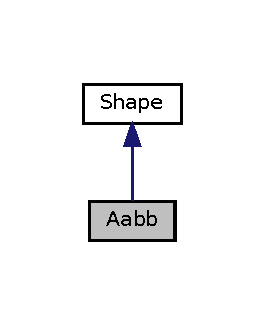
\includegraphics[width=127pt]{classAabb__inherit__graph}
\end{center}
\end{figure}


Collaboration diagram for Aabb\+:
\nopagebreak
\begin{figure}[H]
\begin{center}
\leavevmode
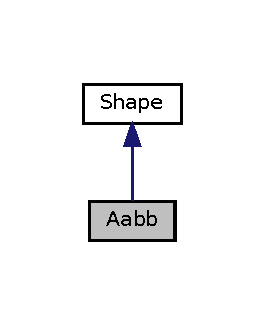
\includegraphics[width=127pt]{classAabb__coll__graph}
\end{center}
\end{figure}
\subsection*{Public Member Functions}
\begin{DoxyCompactItemize}
\item 
\mbox{\Hypertarget{classAabb_a03899715c47e17287f251dc325ebd477}\label{classAabb_a03899715c47e17287f251dc325ebd477}} 
{\bfseries Aabb} (const Vector3 \&min, const Vector3 \&max)
\item 
float \hyperlink{classAabb_ad0f21e16f7be2c42839b0cb025eeed9f}{Get\+Volume} () const
\begin{DoxyCompactList}\small\item\em Computes Volume of the \hyperlink{classAabb}{Aabb}. \end{DoxyCompactList}\item 
float \hyperlink{classAabb_aa5c6fea4dcb0a7f9640a72b1babfe192}{Get\+Surface\+Area} () const
\begin{DoxyCompactList}\small\item\em Computes Surface Area of the \hyperlink{classAabb}{Aabb}. \end{DoxyCompactList}\item 
void \hyperlink{classAabb_a57f19da16237a3e73ba246bd9a20cb9f}{Compute} (const std\+::vector$<$ Vector3 $>$ \&points)
\begin{DoxyCompactList}\small\item\em Initializes this \hyperlink{classAabb}{Aabb} from constructing an \hyperlink{classAabb}{Aabb} that contains all the given points. \end{DoxyCompactList}\item 
virtual bool \hyperlink{classAabb_a98746a9bae7409bd1cf3734125b62da6}{Is\+Intersect} (const \hyperlink{classAabb}{Aabb} \&aabb) const override
\begin{DoxyCompactList}\small\item\em check for collision with another \hyperlink{classAabb}{Aabb} \end{DoxyCompactList}\item 
virtual bool \hyperlink{classAabb_af08568647c234b68334892b20885084a}{Is\+Intersect} (const \hyperlink{classSphere}{Sphere} \&sphere) const override
\begin{DoxyCompactList}\small\item\em Check for collision with a sphere. \end{DoxyCompactList}\item 
bool \hyperlink{classAabb_ac3cca862f5ccbdf7e3aed736476fd9ea}{Contains} (const \hyperlink{classAabb}{Aabb} \&aabb) const
\begin{DoxyCompactList}\small\item\em Check if given \hyperlink{classAabb}{Aabb} fully inside of this \hyperlink{classAabb}{Aabb}. \end{DoxyCompactList}\item 
void \hyperlink{classAabb_ac21813c88f72a56e142c984c3efde368}{Expand} (const Vector3 \&point)
\begin{DoxyCompactList}\small\item\em Expands this \hyperlink{classAabb}{Aabb} to contain also given point. \end{DoxyCompactList}\item 
void \hyperlink{classAabb_ace74b981085cccf12e3ff8e8640a0e07}{Transform} (const Matrix \&transform)
\begin{DoxyCompactList}\small\item\em Compute aabb that would contain the obb of this aabb after transforming it. \end{DoxyCompactList}\item 
Vector3 \hyperlink{classAabb_afe9a77744c815785d6b3c6fa4c3a8340}{Get\+Min} () const
\begin{DoxyCompactList}\small\item\em Get the Min corner of the \hyperlink{classAabb}{Aabb}. \end{DoxyCompactList}\item 
Vector3 \hyperlink{classAabb_ad221f8c84e946375de4c07bdef67e157}{Get\+Max} () const
\begin{DoxyCompactList}\small\item\em Get the Max corner of the \hyperlink{classAabb}{Aabb}. \end{DoxyCompactList}\item 
Vector3 \hyperlink{classAabb_a22fbf825e411bdcbf24c277f1f266d0c}{Get\+Center} () const
\begin{DoxyCompactList}\small\item\em Get the Center of the \hyperlink{classAabb}{Aabb}. \end{DoxyCompactList}\item 
Vector3 \hyperlink{classAabb_a06b1e4e71b018b2e5969f49b460f8ae0}{Get\+Half\+Extent} () const
\begin{DoxyCompactList}\small\item\em Get the Half Extent of the \hyperlink{classAabb}{Aabb}. \end{DoxyCompactList}\end{DoxyCompactItemize}
\subsection*{Static Public Member Functions}
\begin{DoxyCompactItemize}
\item 
static \hyperlink{classAabb}{Aabb} \hyperlink{classAabb_a97ee8719ddae080c16c206f5724b5a9f}{Build\+From\+Center\+And\+Half\+Extents} (const Vector3 \&center, const Vector3 \&half\+Extents)
\begin{DoxyCompactList}\small\item\em Builds \hyperlink{classAabb}{Aabb} from the coordinates of the center of the aabb and the half extent vector to one of the corners. \end{DoxyCompactList}\item 
static \hyperlink{classAabb}{Aabb} \hyperlink{classAabb_a3b8654c48a3713faebbe7490e261eb6e}{Build\+From\+Min\+Max} (const Vector3 \&min, const Vector3 \&max)
\begin{DoxyCompactList}\small\item\em Builds \hyperlink{classAabb}{Aabb} from given aposite corners min and max. \end{DoxyCompactList}\item 
static \hyperlink{classAabb}{Aabb} \hyperlink{classAabb_a32c65313d0c0b6f3918473340cd7c129}{Build\+From\+Local\+A\+A\+B\+B\+And\+Model\+Matrix} (const Matrix \&model\+Matrix, const \hyperlink{classAabb}{Aabb} \&local\+A\+A\+BB)
\begin{DoxyCompactList}\small\item\em Builds \hyperlink{classAabb}{Aabb} around transformed aabb. \end{DoxyCompactList}\item 
static \hyperlink{classAabb}{Aabb} \hyperlink{classAabb_a7f6f3ebe0340505f04b8bf1fc81c7e5f}{Combine} (const \hyperlink{classAabb}{Aabb} \&lhs, const \hyperlink{classAabb}{Aabb} \&rhs)
\begin{DoxyCompactList}\small\item\em Builds an \hyperlink{classAabb}{Aabb} that contains both of the provided Aabbs. \end{DoxyCompactList}\end{DoxyCompactItemize}
\subsection*{Public Attributes}
\begin{DoxyCompactItemize}
\item 
\mbox{\Hypertarget{classAabb_ad97407c0cde4852c9d5b490c1f602302}\label{classAabb_ad97407c0cde4852c9d5b490c1f602302}} 
Vector3 {\bfseries m\+\_\+\+Min}
\item 
\mbox{\Hypertarget{classAabb_a57e862b50109cbaa0e5b731060963bf9}\label{classAabb_a57e862b50109cbaa0e5b731060963bf9}} 
Vector3 {\bfseries m\+\_\+\+Max}
\end{DoxyCompactItemize}


\subsection{Detailed Description}
Axis alligned bounding box, represented by aposite corners min and max. 

\subsection{Member Function Documentation}
\mbox{\Hypertarget{classAabb_a97ee8719ddae080c16c206f5724b5a9f}\label{classAabb_a97ee8719ddae080c16c206f5724b5a9f}} 
\index{Aabb@{Aabb}!Build\+From\+Center\+And\+Half\+Extents@{Build\+From\+Center\+And\+Half\+Extents}}
\index{Build\+From\+Center\+And\+Half\+Extents@{Build\+From\+Center\+And\+Half\+Extents}!Aabb@{Aabb}}
\subsubsection{\texorpdfstring{Build\+From\+Center\+And\+Half\+Extents()}{BuildFromCenterAndHalfExtents()}}
{\footnotesize\ttfamily \hyperlink{classAabb}{Aabb} Aabb\+::\+Build\+From\+Center\+And\+Half\+Extents (\begin{DoxyParamCaption}\item[{const Vector3 \&}]{center,  }\item[{const Vector3 \&}]{half\+Extents }\end{DoxyParamCaption})\hspace{0.3cm}{\ttfamily [static]}}



Builds \hyperlink{classAabb}{Aabb} from the coordinates of the center of the aabb and the half extent vector to one of the corners. 


\begin{DoxyParams}{Parameters}
{\em center} & \\
\hline
{\em half\+Extents} & \\
\hline
\end{DoxyParams}
\begin{DoxyReturn}{Returns}
\hyperlink{classAabb}{Aabb} 
\end{DoxyReturn}
\mbox{\Hypertarget{classAabb_a32c65313d0c0b6f3918473340cd7c129}\label{classAabb_a32c65313d0c0b6f3918473340cd7c129}} 
\index{Aabb@{Aabb}!Build\+From\+Local\+A\+A\+B\+B\+And\+Model\+Matrix@{Build\+From\+Local\+A\+A\+B\+B\+And\+Model\+Matrix}}
\index{Build\+From\+Local\+A\+A\+B\+B\+And\+Model\+Matrix@{Build\+From\+Local\+A\+A\+B\+B\+And\+Model\+Matrix}!Aabb@{Aabb}}
\subsubsection{\texorpdfstring{Build\+From\+Local\+A\+A\+B\+B\+And\+Model\+Matrix()}{BuildFromLocalAABBAndModelMatrix()}}
{\footnotesize\ttfamily \hyperlink{classAabb}{Aabb} Aabb\+::\+Build\+From\+Local\+A\+A\+B\+B\+And\+Model\+Matrix (\begin{DoxyParamCaption}\item[{const Matrix \&}]{model\+Matrix,  }\item[{const \hyperlink{classAabb}{Aabb} \&}]{local\+A\+A\+BB }\end{DoxyParamCaption})\hspace{0.3cm}{\ttfamily [static]}}



Builds \hyperlink{classAabb}{Aabb} around transformed aabb. 


\begin{DoxyParams}{Parameters}
{\em model\+Matrix} & \\
\hline
{\em local\+A\+A\+BB} & \\
\hline
\end{DoxyParams}
\begin{DoxyReturn}{Returns}
\hyperlink{classAabb}{Aabb} 
\end{DoxyReturn}
\mbox{\Hypertarget{classAabb_a3b8654c48a3713faebbe7490e261eb6e}\label{classAabb_a3b8654c48a3713faebbe7490e261eb6e}} 
\index{Aabb@{Aabb}!Build\+From\+Min\+Max@{Build\+From\+Min\+Max}}
\index{Build\+From\+Min\+Max@{Build\+From\+Min\+Max}!Aabb@{Aabb}}
\subsubsection{\texorpdfstring{Build\+From\+Min\+Max()}{BuildFromMinMax()}}
{\footnotesize\ttfamily \hyperlink{classAabb}{Aabb} Aabb\+::\+Build\+From\+Min\+Max (\begin{DoxyParamCaption}\item[{const Vector3 \&}]{min,  }\item[{const Vector3 \&}]{max }\end{DoxyParamCaption})\hspace{0.3cm}{\ttfamily [static]}}



Builds \hyperlink{classAabb}{Aabb} from given aposite corners min and max. 


\begin{DoxyParams}{Parameters}
{\em min} & \\
\hline
{\em max} & \\
\hline
\end{DoxyParams}
\begin{DoxyReturn}{Returns}
\hyperlink{classAabb}{Aabb} 
\end{DoxyReturn}
\mbox{\Hypertarget{classAabb_a7f6f3ebe0340505f04b8bf1fc81c7e5f}\label{classAabb_a7f6f3ebe0340505f04b8bf1fc81c7e5f}} 
\index{Aabb@{Aabb}!Combine@{Combine}}
\index{Combine@{Combine}!Aabb@{Aabb}}
\subsubsection{\texorpdfstring{Combine()}{Combine()}}
{\footnotesize\ttfamily \hyperlink{classAabb}{Aabb} Aabb\+::\+Combine (\begin{DoxyParamCaption}\item[{const \hyperlink{classAabb}{Aabb} \&}]{lhs,  }\item[{const \hyperlink{classAabb}{Aabb} \&}]{rhs }\end{DoxyParamCaption})\hspace{0.3cm}{\ttfamily [static]}}



Builds an \hyperlink{classAabb}{Aabb} that contains both of the provided Aabbs. 


\begin{DoxyParams}{Parameters}
{\em lhs} & \\
\hline
{\em rhs} & \\
\hline
\end{DoxyParams}
\begin{DoxyReturn}{Returns}
\hyperlink{classAabb}{Aabb} 
\end{DoxyReturn}
\mbox{\Hypertarget{classAabb_a57f19da16237a3e73ba246bd9a20cb9f}\label{classAabb_a57f19da16237a3e73ba246bd9a20cb9f}} 
\index{Aabb@{Aabb}!Compute@{Compute}}
\index{Compute@{Compute}!Aabb@{Aabb}}
\subsubsection{\texorpdfstring{Compute()}{Compute()}}
{\footnotesize\ttfamily void Aabb\+::\+Compute (\begin{DoxyParamCaption}\item[{const std\+::vector$<$ Vector3 $>$ \&}]{points }\end{DoxyParamCaption})}



Initializes this \hyperlink{classAabb}{Aabb} from constructing an \hyperlink{classAabb}{Aabb} that contains all the given points. 


\begin{DoxyParams}{Parameters}
{\em points} & \\
\hline
\end{DoxyParams}
\mbox{\Hypertarget{classAabb_ac3cca862f5ccbdf7e3aed736476fd9ea}\label{classAabb_ac3cca862f5ccbdf7e3aed736476fd9ea}} 
\index{Aabb@{Aabb}!Contains@{Contains}}
\index{Contains@{Contains}!Aabb@{Aabb}}
\subsubsection{\texorpdfstring{Contains()}{Contains()}}
{\footnotesize\ttfamily bool Aabb\+::\+Contains (\begin{DoxyParamCaption}\item[{const \hyperlink{classAabb}{Aabb} \&}]{aabb }\end{DoxyParamCaption}) const}



Check if given \hyperlink{classAabb}{Aabb} fully inside of this \hyperlink{classAabb}{Aabb}. 


\begin{DoxyParams}{Parameters}
{\em aabb} & \\
\hline
\end{DoxyParams}
\begin{DoxyReturn}{Returns}
true if this aabb contains given aabb 

false otherwise 
\end{DoxyReturn}
\mbox{\Hypertarget{classAabb_ac21813c88f72a56e142c984c3efde368}\label{classAabb_ac21813c88f72a56e142c984c3efde368}} 
\index{Aabb@{Aabb}!Expand@{Expand}}
\index{Expand@{Expand}!Aabb@{Aabb}}
\subsubsection{\texorpdfstring{Expand()}{Expand()}}
{\footnotesize\ttfamily void Aabb\+::\+Expand (\begin{DoxyParamCaption}\item[{const Vector3 \&}]{point }\end{DoxyParamCaption})}



Expands this \hyperlink{classAabb}{Aabb} to contain also given point. 


\begin{DoxyParams}{Parameters}
{\em point} & \\
\hline
\end{DoxyParams}
\mbox{\Hypertarget{classAabb_a22fbf825e411bdcbf24c277f1f266d0c}\label{classAabb_a22fbf825e411bdcbf24c277f1f266d0c}} 
\index{Aabb@{Aabb}!Get\+Center@{Get\+Center}}
\index{Get\+Center@{Get\+Center}!Aabb@{Aabb}}
\subsubsection{\texorpdfstring{Get\+Center()}{GetCenter()}}
{\footnotesize\ttfamily Vector3 Aabb\+::\+Get\+Center (\begin{DoxyParamCaption}{ }\end{DoxyParamCaption}) const}



Get the Center of the \hyperlink{classAabb}{Aabb}. 

\begin{DoxyReturn}{Returns}
Vector3 
\end{DoxyReturn}
\mbox{\Hypertarget{classAabb_a06b1e4e71b018b2e5969f49b460f8ae0}\label{classAabb_a06b1e4e71b018b2e5969f49b460f8ae0}} 
\index{Aabb@{Aabb}!Get\+Half\+Extent@{Get\+Half\+Extent}}
\index{Get\+Half\+Extent@{Get\+Half\+Extent}!Aabb@{Aabb}}
\subsubsection{\texorpdfstring{Get\+Half\+Extent()}{GetHalfExtent()}}
{\footnotesize\ttfamily Vector3 Aabb\+::\+Get\+Half\+Extent (\begin{DoxyParamCaption}{ }\end{DoxyParamCaption}) const}



Get the Half Extent of the \hyperlink{classAabb}{Aabb}. 

\begin{DoxyReturn}{Returns}
Vector3 
\end{DoxyReturn}
\mbox{\Hypertarget{classAabb_ad221f8c84e946375de4c07bdef67e157}\label{classAabb_ad221f8c84e946375de4c07bdef67e157}} 
\index{Aabb@{Aabb}!Get\+Max@{Get\+Max}}
\index{Get\+Max@{Get\+Max}!Aabb@{Aabb}}
\subsubsection{\texorpdfstring{Get\+Max()}{GetMax()}}
{\footnotesize\ttfamily Vector3 Aabb\+::\+Get\+Max (\begin{DoxyParamCaption}{ }\end{DoxyParamCaption}) const}



Get the Max corner of the \hyperlink{classAabb}{Aabb}. 

\begin{DoxyReturn}{Returns}
Vector3 
\end{DoxyReturn}
\mbox{\Hypertarget{classAabb_afe9a77744c815785d6b3c6fa4c3a8340}\label{classAabb_afe9a77744c815785d6b3c6fa4c3a8340}} 
\index{Aabb@{Aabb}!Get\+Min@{Get\+Min}}
\index{Get\+Min@{Get\+Min}!Aabb@{Aabb}}
\subsubsection{\texorpdfstring{Get\+Min()}{GetMin()}}
{\footnotesize\ttfamily Vector3 Aabb\+::\+Get\+Min (\begin{DoxyParamCaption}{ }\end{DoxyParamCaption}) const}



Get the Min corner of the \hyperlink{classAabb}{Aabb}. 

\begin{DoxyReturn}{Returns}
Vector3 
\end{DoxyReturn}
\mbox{\Hypertarget{classAabb_aa5c6fea4dcb0a7f9640a72b1babfe192}\label{classAabb_aa5c6fea4dcb0a7f9640a72b1babfe192}} 
\index{Aabb@{Aabb}!Get\+Surface\+Area@{Get\+Surface\+Area}}
\index{Get\+Surface\+Area@{Get\+Surface\+Area}!Aabb@{Aabb}}
\subsubsection{\texorpdfstring{Get\+Surface\+Area()}{GetSurfaceArea()}}
{\footnotesize\ttfamily float Aabb\+::\+Get\+Surface\+Area (\begin{DoxyParamCaption}{ }\end{DoxyParamCaption}) const}



Computes Surface Area of the \hyperlink{classAabb}{Aabb}. 

\begin{DoxyReturn}{Returns}
float 
\end{DoxyReturn}
\mbox{\Hypertarget{classAabb_ad0f21e16f7be2c42839b0cb025eeed9f}\label{classAabb_ad0f21e16f7be2c42839b0cb025eeed9f}} 
\index{Aabb@{Aabb}!Get\+Volume@{Get\+Volume}}
\index{Get\+Volume@{Get\+Volume}!Aabb@{Aabb}}
\subsubsection{\texorpdfstring{Get\+Volume()}{GetVolume()}}
{\footnotesize\ttfamily float Aabb\+::\+Get\+Volume (\begin{DoxyParamCaption}{ }\end{DoxyParamCaption}) const}



Computes Volume of the \hyperlink{classAabb}{Aabb}. 

\begin{DoxyReturn}{Returns}
float 
\end{DoxyReturn}
\mbox{\Hypertarget{classAabb_a98746a9bae7409bd1cf3734125b62da6}\label{classAabb_a98746a9bae7409bd1cf3734125b62da6}} 
\index{Aabb@{Aabb}!Is\+Intersect@{Is\+Intersect}}
\index{Is\+Intersect@{Is\+Intersect}!Aabb@{Aabb}}
\subsubsection{\texorpdfstring{Is\+Intersect()}{IsIntersect()}\hspace{0.1cm}{\footnotesize\ttfamily [1/2]}}
{\footnotesize\ttfamily bool Aabb\+::\+Is\+Intersect (\begin{DoxyParamCaption}\item[{const \hyperlink{classAabb}{Aabb} \&}]{aabb }\end{DoxyParamCaption}) const\hspace{0.3cm}{\ttfamily [override]}, {\ttfamily [virtual]}}



check for collision with another \hyperlink{classAabb}{Aabb} 


\begin{DoxyParams}{Parameters}
{\em aabb} & \\
\hline
\end{DoxyParams}
\begin{DoxyReturn}{Returns}
true if intersects 

false if not intersects 
\end{DoxyReturn}


Implements \hyperlink{classShape_a1bfc3d6c995c4326d4691b22d16d2f12}{Shape}.

\mbox{\Hypertarget{classAabb_af08568647c234b68334892b20885084a}\label{classAabb_af08568647c234b68334892b20885084a}} 
\index{Aabb@{Aabb}!Is\+Intersect@{Is\+Intersect}}
\index{Is\+Intersect@{Is\+Intersect}!Aabb@{Aabb}}
\subsubsection{\texorpdfstring{Is\+Intersect()}{IsIntersect()}\hspace{0.1cm}{\footnotesize\ttfamily [2/2]}}
{\footnotesize\ttfamily bool Aabb\+::\+Is\+Intersect (\begin{DoxyParamCaption}\item[{const \hyperlink{classSphere}{Sphere} \&}]{sphere }\end{DoxyParamCaption}) const\hspace{0.3cm}{\ttfamily [override]}, {\ttfamily [virtual]}}



Check for collision with a sphere. 


\begin{DoxyParams}{Parameters}
{\em sphere} & \\
\hline
\end{DoxyParams}
\begin{DoxyReturn}{Returns}
true if intersects 

false if not intersects 
\end{DoxyReturn}


Implements \hyperlink{classShape_a1c942dca54e0d81f685624f33f2ce6c8}{Shape}.

\mbox{\Hypertarget{classAabb_ace74b981085cccf12e3ff8e8640a0e07}\label{classAabb_ace74b981085cccf12e3ff8e8640a0e07}} 
\index{Aabb@{Aabb}!Transform@{Transform}}
\index{Transform@{Transform}!Aabb@{Aabb}}
\subsubsection{\texorpdfstring{Transform()}{Transform()}}
{\footnotesize\ttfamily void Aabb\+::\+Transform (\begin{DoxyParamCaption}\item[{const Matrix \&}]{transform }\end{DoxyParamCaption})}



Compute aabb that would contain the obb of this aabb after transforming it. 


\begin{DoxyParams}{Parameters}
{\em transform} & \\
\hline
\end{DoxyParams}


The documentation for this class was generated from the following files\+:\begin{DoxyCompactItemize}
\item 
Physics/\+Geometry/\hyperlink{Aabb_8h}{Aabb.\+h}\item 
Physics/\+Geometry/\hyperlink{Aabb_8cpp}{Aabb.\+cpp}\end{DoxyCompactItemize}

\hypertarget{structAnimation}{}\section{Animation Struct Reference}
\label{structAnimation}\index{Animation@{Animation}}


Describes a keyframe animation for a skeleton.  




{\ttfamily \#include $<$Animation.\+h$>$}



Collaboration diagram for Animation\+:
\nopagebreak
\begin{figure}[H]
\begin{center}
\leavevmode
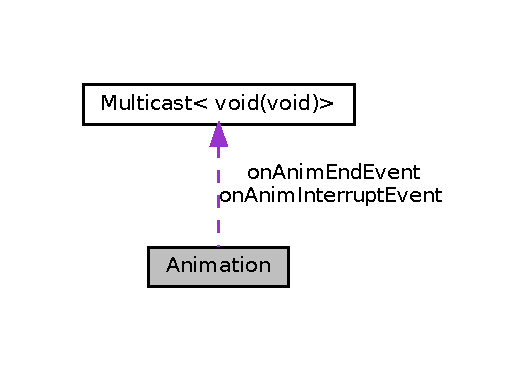
\includegraphics[width=253pt]{structAnimation__coll__graph}
\end{center}
\end{figure}
\subsection*{Public Types}
\begin{DoxyCompactItemize}
\item 
\mbox{\Hypertarget{structAnimation_ac07104f8333840b8c2fca7fe620ace19}\label{structAnimation_ac07104f8333840b8c2fca7fe620ace19}} 
typedef \hyperlink{classMulticast}{Multicast}$<$ void(void)$>$ \hyperlink{structAnimation_ac07104f8333840b8c2fca7fe620ace19}{Anim\+Multicast}
\begin{DoxyCompactList}\small\item\em Typedef used to define animation events (stored in a multicast form) \end{DoxyCompactList}\end{DoxyCompactItemize}
\subsection*{Public Member Functions}
\begin{DoxyCompactItemize}
\item 
\mbox{\Hypertarget{structAnimation_ae4eef1e6d0194258f4bf2a6bbcc874f5}\label{structAnimation_ae4eef1e6d0194258f4bf2a6bbcc874f5}} 
void \hyperlink{structAnimation_ae4eef1e6d0194258f4bf2a6bbcc874f5}{Events\+Setup} ()
\begin{DoxyCompactList}\small\item\em Setups the animation event\textquotesingle{}s vector so it is of the right size. \end{DoxyCompactList}\item 
void \hyperlink{structAnimation_a0b4ff938810fc4f137b004b2a04d3c1d}{Add\+Anim\+Event} (int tick, sol\+::table entry)
\begin{DoxyCompactList}\small\item\em Used for adding an animation event from L\+UA script. \end{DoxyCompactList}\item 
void \hyperlink{structAnimation_a724a8cd4b9958010758cd76a88a7853d}{Add\+Anim\+End\+Event} (sol\+::table entry)
\begin{DoxyCompactList}\small\item\em Used for adding an animation to the end. \end{DoxyCompactList}\item 
void \hyperlink{structAnimation_a8178c273c3890085c4a39da1fb1531fb}{Add\+Interrupt\+Event} (sol\+::table entry)
\begin{DoxyCompactList}\small\item\em \hyperlink{classEvent}{Event} that fires when a transition interrupts this animation. \end{DoxyCompactList}\item 
void \hyperlink{structAnimation_a4bfa0e66492903e4435233193ad4979a}{Call\+Event} (float anim\+Time)
\begin{DoxyCompactList}\small\item\em Fires an animation event (if there is one) \end{DoxyCompactList}\end{DoxyCompactItemize}
\subsection*{Public Attributes}
\begin{DoxyCompactItemize}
\item 
\mbox{\Hypertarget{structAnimation_a0447169235a9232787743cd944752b3f}\label{structAnimation_a0447169235a9232787743cd944752b3f}} 
std\+::string \hyperlink{structAnimation_a0447169235a9232787743cd944752b3f}{anim\+Name}
\begin{DoxyCompactList}\small\item\em \hyperlink{structAnimation}{Animation} name. \end{DoxyCompactList}\item 
\mbox{\Hypertarget{structAnimation_a66cc7333638f071b0401072ba95c55fd}\label{structAnimation_a66cc7333638f071b0401072ba95c55fd}} 
float \hyperlink{structAnimation_a66cc7333638f071b0401072ba95c55fd}{duration}
\begin{DoxyCompactList}\small\item\em Duration in ticks. \end{DoxyCompactList}\item 
\mbox{\Hypertarget{structAnimation_a929555773b65c756af1519fc39317560}\label{structAnimation_a929555773b65c756af1519fc39317560}} 
float \hyperlink{structAnimation_a929555773b65c756af1519fc39317560}{ticks\+Per\+Second}
\begin{DoxyCompactList}\small\item\em Ticks per second (to transform between ticks and seconds or other units) \end{DoxyCompactList}\item 
\mbox{\Hypertarget{structAnimation_aad5027023051d9891c36539a27e2df3d}\label{structAnimation_aad5027023051d9891c36539a27e2df3d}} 
bool \hyperlink{structAnimation_aad5027023051d9891c36539a27e2df3d}{loops}
\begin{DoxyCompactList}\small\item\em If this animation loops or not. \end{DoxyCompactList}\item 
\mbox{\Hypertarget{structAnimation_a20f3a503b821838808d517a2230c4b94}\label{structAnimation_a20f3a503b821838808d517a2230c4b94}} 
std\+::vector$<$ \hyperlink{structAnimation_ac07104f8333840b8c2fca7fe620ace19}{Anim\+Multicast} $>$ \hyperlink{structAnimation_a20f3a503b821838808d517a2230c4b94}{animation\+Events}
\begin{DoxyCompactList}\small\item\em Vector of animation events, potentially one per keyframe. \end{DoxyCompactList}\item 
\mbox{\Hypertarget{structAnimation_a8f971c5370b646d026147098db0bd66b}\label{structAnimation_a8f971c5370b646d026147098db0bd66b}} 
\hyperlink{structAnimation_ac07104f8333840b8c2fca7fe620ace19}{Anim\+Multicast} \hyperlink{structAnimation_a8f971c5370b646d026147098db0bd66b}{on\+Anim\+End\+Event}
\begin{DoxyCompactList}\small\item\em This will fire if the animation ends. \end{DoxyCompactList}\item 
\mbox{\Hypertarget{structAnimation_a589b561e4143d544f9d3eb678650efd1}\label{structAnimation_a589b561e4143d544f9d3eb678650efd1}} 
\hyperlink{structAnimation_ac07104f8333840b8c2fca7fe620ace19}{Anim\+Multicast} \hyperlink{structAnimation_a589b561e4143d544f9d3eb678650efd1}{on\+Anim\+Interrupt\+Event}
\begin{DoxyCompactList}\small\item\em This will fire if the animation is interrupted. \end{DoxyCompactList}\item 
\mbox{\Hypertarget{structAnimation_a929158d26b6d71f1d297820625e46fc7}\label{structAnimation_a929158d26b6d71f1d297820625e46fc7}} 
std\+::vector$<$ \hyperlink{structAnimChannel}{Anim\+Channel} $>$ \hyperlink{structAnimation_a929158d26b6d71f1d297820625e46fc7}{channels}
\begin{DoxyCompactList}\small\item\em Vector of animation channels. Each channel has information about which bone is animated and its keyframe information. \end{DoxyCompactList}\item 
\mbox{\Hypertarget{structAnimation_ab0ec7a6ccca71fc844b62e2309a7a539}\label{structAnimation_ab0ec7a6ccca71fc844b62e2309a7a539}} 
std\+::unordered\+\_\+map$<$ std\+::string, \hyperlink{structAnimChannel}{Anim\+Channel} $>$ \hyperlink{structAnimation_ab0ec7a6ccca71fc844b62e2309a7a539}{bone\+Channel\+Map}
\begin{DoxyCompactList}\small\item\em Hash table for bone channels. \end{DoxyCompactList}\end{DoxyCompactItemize}


\subsection{Detailed Description}
Describes a keyframe animation for a skeleton. 

\subsection{Member Function Documentation}
\mbox{\Hypertarget{structAnimation_a724a8cd4b9958010758cd76a88a7853d}\label{structAnimation_a724a8cd4b9958010758cd76a88a7853d}} 
\index{Animation@{Animation}!Add\+Anim\+End\+Event@{Add\+Anim\+End\+Event}}
\index{Add\+Anim\+End\+Event@{Add\+Anim\+End\+Event}!Animation@{Animation}}
\subsubsection{\texorpdfstring{Add\+Anim\+End\+Event()}{AddAnimEndEvent()}}
{\footnotesize\ttfamily void Animation\+::\+Add\+Anim\+End\+Event (\begin{DoxyParamCaption}\item[{sol\+::table}]{entry }\end{DoxyParamCaption})\hspace{0.3cm}{\ttfamily [inline]}}



Used for adding an animation to the end. 


\begin{DoxyParams}{Parameters}
{\em entry} & Table which contains the lua self reference and the method it has to run \\
\hline
\end{DoxyParams}
\mbox{\Hypertarget{structAnimation_a0b4ff938810fc4f137b004b2a04d3c1d}\label{structAnimation_a0b4ff938810fc4f137b004b2a04d3c1d}} 
\index{Animation@{Animation}!Add\+Anim\+Event@{Add\+Anim\+Event}}
\index{Add\+Anim\+Event@{Add\+Anim\+Event}!Animation@{Animation}}
\subsubsection{\texorpdfstring{Add\+Anim\+Event()}{AddAnimEvent()}}
{\footnotesize\ttfamily void Animation\+::\+Add\+Anim\+Event (\begin{DoxyParamCaption}\item[{int}]{tick,  }\item[{sol\+::table}]{entry }\end{DoxyParamCaption})\hspace{0.3cm}{\ttfamily [inline]}}



Used for adding an animation event from L\+UA script. 


\begin{DoxyParams}{Parameters}
{\em tick} & Which tick we want this event to happen \\
\hline
{\em entry} & Table which contains the lua self reference and the method it has to run \\
\hline
\end{DoxyParams}
\mbox{\Hypertarget{structAnimation_a8178c273c3890085c4a39da1fb1531fb}\label{structAnimation_a8178c273c3890085c4a39da1fb1531fb}} 
\index{Animation@{Animation}!Add\+Interrupt\+Event@{Add\+Interrupt\+Event}}
\index{Add\+Interrupt\+Event@{Add\+Interrupt\+Event}!Animation@{Animation}}
\subsubsection{\texorpdfstring{Add\+Interrupt\+Event()}{AddInterruptEvent()}}
{\footnotesize\ttfamily void Animation\+::\+Add\+Interrupt\+Event (\begin{DoxyParamCaption}\item[{sol\+::table}]{entry }\end{DoxyParamCaption})\hspace{0.3cm}{\ttfamily [inline]}}



\hyperlink{classEvent}{Event} that fires when a transition interrupts this animation. 


\begin{DoxyParams}{Parameters}
{\em entry} & Table which contains the lua self reference and the method it has to run \\
\hline
\end{DoxyParams}
\mbox{\Hypertarget{structAnimation_a4bfa0e66492903e4435233193ad4979a}\label{structAnimation_a4bfa0e66492903e4435233193ad4979a}} 
\index{Animation@{Animation}!Call\+Event@{Call\+Event}}
\index{Call\+Event@{Call\+Event}!Animation@{Animation}}
\subsubsection{\texorpdfstring{Call\+Event()}{CallEvent()}}
{\footnotesize\ttfamily void Animation\+::\+Call\+Event (\begin{DoxyParamCaption}\item[{float}]{anim\+Time }\end{DoxyParamCaption})\hspace{0.3cm}{\ttfamily [inline]}}



Fires an animation event (if there is one) 


\begin{DoxyParams}{Parameters}
{\em anim\+Time} & \\
\hline
\end{DoxyParams}


The documentation for this struct was generated from the following file\+:\begin{DoxyCompactItemize}
\item 
Animation/\hyperlink{Animation_8h}{Animation.\+h}\end{DoxyCompactItemize}

\hypertarget{classAnimationComponent}{}\section{Animation\+Component Class Reference}
\label{classAnimationComponent}\index{Animation\+Component@{Animation\+Component}}


Inheritance diagram for Animation\+Component\+:\nopagebreak
\begin{figure}[H]
\begin{center}
\leavevmode
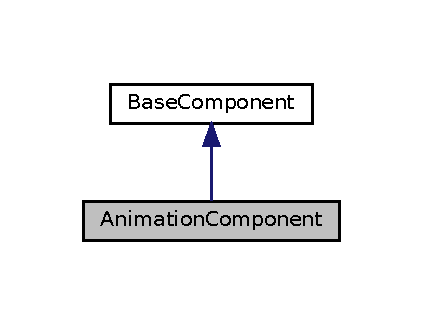
\includegraphics[width=203pt]{classAnimationComponent__inherit__graph}
\end{center}
\end{figure}


Collaboration diagram for Animation\+Component\+:\nopagebreak
\begin{figure}[H]
\begin{center}
\leavevmode
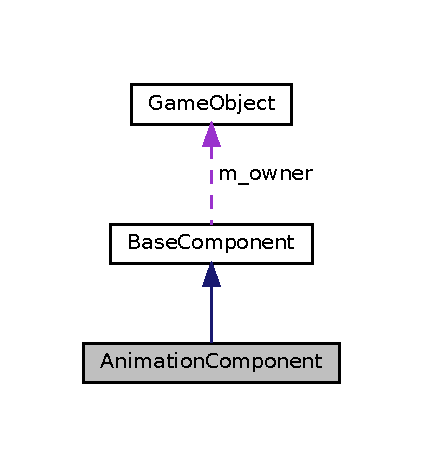
\includegraphics[width=203pt]{classAnimationComponent__coll__graph}
\end{center}
\end{figure}
\subsection*{Public Member Functions}
\begin{DoxyCompactItemize}
\item 
\mbox{\Hypertarget{classAnimationComponent_a2759aea8d6d3e70f7b4f0f91eb68dbf2}\label{classAnimationComponent_a2759aea8d6d3e70f7b4f0f91eb68dbf2}} 
{\bfseries Animation\+Component} (\hyperlink{classGameObject}{Game\+Object} $\ast$owner)
\item 
\mbox{\Hypertarget{classAnimationComponent_a7847ca35ed87a7d2156081ad41822de4}\label{classAnimationComponent_a7847ca35ed87a7d2156081ad41822de4}} 
virtual void {\bfseries Init} (\hyperlink{classResourceManager}{Resource\+Manager} $\ast$res, \hyperlink{classDXRenderer}{D\+X\+Renderer} $\ast$dxrenderer)
\item 
\mbox{\Hypertarget{classAnimationComponent_ab079696aad04351fa60a12040aeffe58}\label{classAnimationComponent_ab079696aad04351fa60a12040aeffe58}} 
virtual void {\bfseries Begin} (\hyperlink{classGameObjectManager}{Game\+Object\+Manager} $\ast$go\+Mgr)
\item 
\mbox{\Hypertarget{classAnimationComponent_a03636b1eaab7e1a4aaf05d6321ad2478}\label{classAnimationComponent_a03636b1eaab7e1a4aaf05d6321ad2478}} 
void \hyperlink{classAnimationComponent_a03636b1eaab7e1a4aaf05d6321ad2478}{Animation\+End} (\hyperlink{structAnimState}{Anim\+State} $\ast$anim)
\begin{DoxyCompactList}\small\item\em void Switch\+Animation(std\+::string const\& anim\+Name, float trans\+Duration); \end{DoxyCompactList}\item 
\mbox{\Hypertarget{classAnimationComponent_af826696c15c75e727360009e1ebd4d8d}\label{classAnimationComponent_af826696c15c75e727360009e1ebd4d8d}} 
void {\bfseries Set\+Trigger} (std\+::string const \&trigger)
\item 
\mbox{\Hypertarget{classAnimationComponent_afd02daaa324cf1a038aed3736c579f81}\label{classAnimationComponent_afd02daaa324cf1a038aed3736c579f81}} 
\hyperlink{structAnimState}{Anim\+State} $\ast$ {\bfseries Create\+State} (std\+::string state\+Name, std\+::string anim\+Name, float speed)
\item 
\mbox{\Hypertarget{classAnimationComponent_ad19e6c6a3b266d7987391be6d3ece4ea}\label{classAnimationComponent_ad19e6c6a3b266d7987391be6d3ece4ea}} 
\hyperlink{structAnimState}{Anim\+State} $\ast$ {\bfseries Create\+State} (std\+::string state\+Name, std\+::string anim\+Name)
\item 
\mbox{\Hypertarget{classAnimationComponent_ae63c07831f76d1c69a8be6dbd03f54a2}\label{classAnimationComponent_ae63c07831f76d1c69a8be6dbd03f54a2}} 
void {\bfseries Set\+Entry\+State} (\hyperlink{structAnimState}{Anim\+State} $\ast$entry)
\end{DoxyCompactItemize}
\subsection*{Static Public Attributes}
\begin{DoxyCompactItemize}
\item 
\mbox{\Hypertarget{classAnimationComponent_afd0771d0bf533c347cb80f0343ec747b}\label{classAnimationComponent_afd0771d0bf533c347cb80f0343ec747b}} 
static Component\+Id const {\bfseries static\+\_\+type} = Base\+Component\+::number\+Of\+Types++
\end{DoxyCompactItemize}
\subsection*{Friends}
\begin{DoxyCompactItemize}
\item 
\mbox{\Hypertarget{classAnimationComponent_a328c093d609680cca505905c6d49901a}\label{classAnimationComponent_a328c093d609680cca505905c6d49901a}} 
class {\bfseries Factory}
\item 
\mbox{\Hypertarget{classAnimationComponent_ab3d6fafb2064bace492fd6b503d044f4}\label{classAnimationComponent_ab3d6fafb2064bace492fd6b503d044f4}} 
class {\bfseries Scripting\+Manager}
\item 
\mbox{\Hypertarget{classAnimationComponent_a4c8fb761c777f1a874c5d97e052686ad}\label{classAnimationComponent_a4c8fb761c777f1a874c5d97e052686ad}} 
class {\bfseries Animation\+System}
\end{DoxyCompactItemize}
\subsection*{Additional Inherited Members}


The documentation for this class was generated from the following files\+:\begin{DoxyCompactItemize}
\item 
Components/Animation\+Component.\+h\item 
Components/Animation\+Component.\+cpp\end{DoxyCompactItemize}

\hypertarget{classAnimationSystem}{}\section{Animation\+System Class Reference}
\label{classAnimationSystem}\index{Animation\+System@{Animation\+System}}


Inheritance diagram for Animation\+System\+:
\nopagebreak
\begin{figure}[H]
\begin{center}
\leavevmode
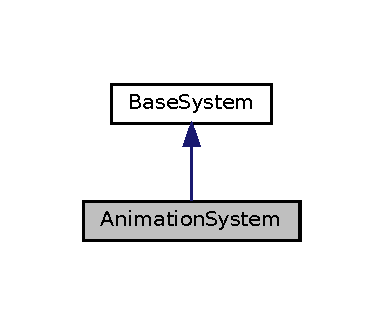
\includegraphics[width=184pt]{classAnimationSystem__inherit__graph}
\end{center}
\end{figure}


Collaboration diagram for Animation\+System\+:
\nopagebreak
\begin{figure}[H]
\begin{center}
\leavevmode
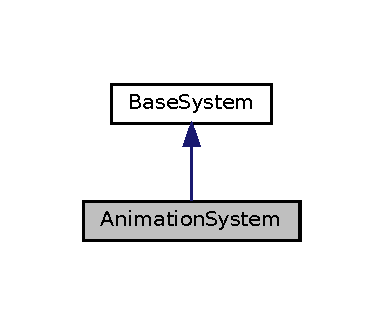
\includegraphics[width=184pt]{classAnimationSystem__coll__graph}
\end{center}
\end{figure}
\subsection*{Public Member Functions}
\begin{DoxyCompactItemize}
\item 
virtual void \hyperlink{classAnimationSystem_a887b7a3f1fa8d9c425b6ba49e12a3ca4}{Register\+\_\+\+Game\+Object} (\hyperlink{classGameObject}{Game\+Object} $\ast$go)
\begin{DoxyCompactList}\small\item\em Registers \hyperlink{classGameObject}{Game\+Object} GO in this system. \end{DoxyCompactList}\item 
virtual void \hyperlink{classAnimationSystem_aa74600f86761b9bb47a0689665901a49}{Update} (float dt, \hyperlink{structBaseSystemCompNode}{Base\+System\+Comp\+Node} $\ast$comp\+Node)
\begin{DoxyCompactList}\small\item\em Regular Update call. Called once per registered \hyperlink{classGameObject}{Game\+Object} by Update\+All\+Nodes. \end{DoxyCompactList}\end{DoxyCompactItemize}
\subsection*{Static Public Attributes}
\begin{DoxyCompactItemize}
\item 
\mbox{\Hypertarget{classAnimationSystem_a288581c9524350d393f2a93e5aeb3165}\label{classAnimationSystem_a288581c9524350d393f2a93e5aeb3165}} 
static unsigned int const {\bfseries static\+\_\+type} = \hyperlink{classBaseSystem_a7ef356edab3cfb02905e0a73a645b131}{Base\+System\+::number\+Of\+Types}++
\end{DoxyCompactItemize}
\subsection*{Additional Inherited Members}


\subsection{Member Function Documentation}
\mbox{\Hypertarget{classAnimationSystem_a887b7a3f1fa8d9c425b6ba49e12a3ca4}\label{classAnimationSystem_a887b7a3f1fa8d9c425b6ba49e12a3ca4}} 
\index{Animation\+System@{Animation\+System}!Register\+\_\+\+Game\+Object@{Register\+\_\+\+Game\+Object}}
\index{Register\+\_\+\+Game\+Object@{Register\+\_\+\+Game\+Object}!Animation\+System@{Animation\+System}}
\subsubsection{\texorpdfstring{Register\+\_\+\+Game\+Object()}{Register\_GameObject()}}
{\footnotesize\ttfamily void Animation\+System\+::\+Register\+\_\+\+Game\+Object (\begin{DoxyParamCaption}\item[{\hyperlink{classGameObject}{Game\+Object} $\ast$}]{go }\end{DoxyParamCaption})\hspace{0.3cm}{\ttfamily [virtual]}}



Registers \hyperlink{classGameObject}{Game\+Object} GO in this system. 


\begin{DoxyParams}{Parameters}
{\em go} & \\
\hline
\end{DoxyParams}


Implements \hyperlink{classBaseSystem}{Base\+System}.

\mbox{\Hypertarget{classAnimationSystem_aa74600f86761b9bb47a0689665901a49}\label{classAnimationSystem_aa74600f86761b9bb47a0689665901a49}} 
\index{Animation\+System@{Animation\+System}!Update@{Update}}
\index{Update@{Update}!Animation\+System@{Animation\+System}}
\subsubsection{\texorpdfstring{Update()}{Update()}}
{\footnotesize\ttfamily void Animation\+System\+::\+Update (\begin{DoxyParamCaption}\item[{float}]{dt,  }\item[{\hyperlink{structBaseSystemCompNode}{Base\+System\+Comp\+Node} $\ast$}]{comp\+Node }\end{DoxyParamCaption})\hspace{0.3cm}{\ttfamily [virtual]}}



Regular Update call. Called once per registered \hyperlink{classGameObject}{Game\+Object} by Update\+All\+Nodes. 


\begin{DoxyParams}{Parameters}
{\em dt} & \\
\hline
{\em comp\+Node} & \\
\hline
\end{DoxyParams}


Reimplemented from \hyperlink{classBaseSystem_a465191589a1ef8b8f3a8e20fa4656d47}{Base\+System}.



The documentation for this class was generated from the following files\+:\begin{DoxyCompactItemize}
\item 
Systems/Animation\+System.\+h\item 
Systems/Animation\+System.\+cpp\end{DoxyCompactItemize}

\hypertarget{structAnimatorCompNode}{}\section{Animator\+Comp\+Node Struct Reference}
\label{structAnimatorCompNode}\index{Animator\+Comp\+Node@{Animator\+Comp\+Node}}


T\+E\+ST S\+Y\+S\+T\+EM, W\+I\+LL R\+E\+Q\+U\+I\+RE A T\+R\+A\+N\+S\+F\+O\+RM A\+ND R\+E\+N\+D\+E\+R\+ER C\+O\+MP.  




{\ttfamily \#include $<$Animation\+System.\+h$>$}



Inheritance diagram for Animator\+Comp\+Node\+:
\nopagebreak
\begin{figure}[H]
\begin{center}
\leavevmode
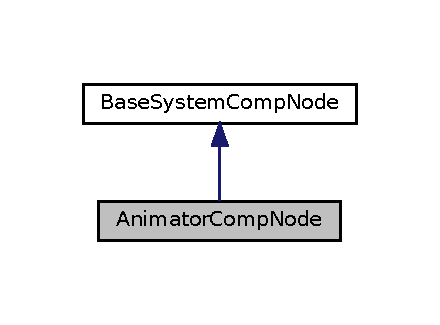
\includegraphics[width=211pt]{structAnimatorCompNode__inherit__graph}
\end{center}
\end{figure}


Collaboration diagram for Animator\+Comp\+Node\+:
\nopagebreak
\begin{figure}[H]
\begin{center}
\leavevmode
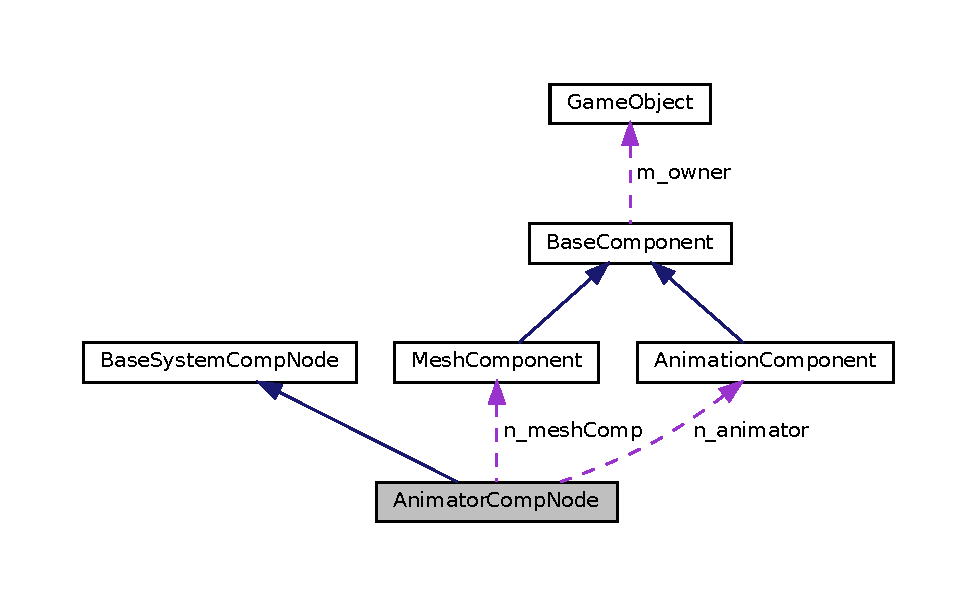
\includegraphics[width=350pt]{structAnimatorCompNode__coll__graph}
\end{center}
\end{figure}
\subsection*{Public Member Functions}
\begin{DoxyCompactItemize}
\item 
\mbox{\Hypertarget{structAnimatorCompNode_a9f5b09f07667bc70a032bef987c0520e}\label{structAnimatorCompNode_a9f5b09f07667bc70a032bef987c0520e}} 
{\bfseries Animator\+Comp\+Node} (\hyperlink{classAnimationComponent}{Animation\+Component} $\ast$animator, \hyperlink{classMeshComponent}{Mesh\+Component} $\ast$mesh\+Comp)
\end{DoxyCompactItemize}
\subsection*{Public Attributes}
\begin{DoxyCompactItemize}
\item 
\mbox{\Hypertarget{structAnimatorCompNode_a1c64b315bbb562b2c8f60a6312cdb5d2}\label{structAnimatorCompNode_a1c64b315bbb562b2c8f60a6312cdb5d2}} 
\hyperlink{classAnimationComponent}{Animation\+Component} $\ast$ {\bfseries n\+\_\+animator}
\item 
\mbox{\Hypertarget{structAnimatorCompNode_a4276b03a7b4bf28ca260170955afd71f}\label{structAnimatorCompNode_a4276b03a7b4bf28ca260170955afd71f}} 
\hyperlink{classMeshComponent}{Mesh\+Component} $\ast$ {\bfseries n\+\_\+mesh\+Comp}
\end{DoxyCompactItemize}


\subsection{Detailed Description}
T\+E\+ST S\+Y\+S\+T\+EM, W\+I\+LL R\+E\+Q\+U\+I\+RE A T\+R\+A\+N\+S\+F\+O\+RM A\+ND R\+E\+N\+D\+E\+R\+ER C\+O\+MP. 

The documentation for this struct was generated from the following file\+:\begin{DoxyCompactItemize}
\item 
Systems/Animation\+System.\+h\end{DoxyCompactItemize}

\hypertarget{classAnimatorController}{}\section{Animator\+Controller Class Reference}
\label{classAnimatorController}\index{Animator\+Controller@{Animator\+Controller}}


Class that represents the animation state machine itself.  




{\ttfamily \#include $<$Animator\+Controller.\+h$>$}

\subsection*{Public Member Functions}
\begin{DoxyCompactItemize}
\item 
\hyperlink{classAnimatorController_a9b32e8e7a4b72e80c6ae7a88fc961c4e}{Animator\+Controller} ()
\begin{DoxyCompactList}\small\item\em Construct a new Animator Controller object. \end{DoxyCompactList}\item 
\mbox{\Hypertarget{classAnimatorController_a9f96c39d24c29d96c6d343737411c0bd}\label{classAnimatorController_a9f96c39d24c29d96c6d343737411c0bd}} 
\hyperlink{classAnimatorController_a9f96c39d24c29d96c6d343737411c0bd}{$\sim$\+Animator\+Controller} ()
\begin{DoxyCompactList}\small\item\em Destroy the Animator Controller object. \end{DoxyCompactList}\item 
\hyperlink{structAnimState}{Anim\+State} $\ast$ \hyperlink{classAnimatorController_ae84a0064dd344fb2a2b4bb6de69557e1}{Get\+Current\+State} () const
\begin{DoxyCompactList}\small\item\em Get the Current \hyperlink{classState}{State} on the state machine. \end{DoxyCompactList}\item 
\hyperlink{structAnimState}{Anim\+State} $\ast$ \hyperlink{classAnimatorController_aa2b6d02748cb880d596122448f685f9f}{Get\+State} (std\+::string const \&name) const
\begin{DoxyCompactList}\small\item\em Get a state of name equal to parameter name. \end{DoxyCompactList}\item 
bool \hyperlink{classAnimatorController_ac079dc6e19c4284fa941033577ddd45d}{Is\+State\+Name\+Valid} (std\+::string const \&name)
\begin{DoxyCompactList}\small\item\em Returns true if the name for the state is valid. \end{DoxyCompactList}\item 
void \hyperlink{classAnimatorController_a7e2acba88b4bc663c3bc3a04c20962c8}{Add\+State} (\hyperlink{structAnimState}{Anim\+State} $\ast$new\+State)
\begin{DoxyCompactList}\small\item\em Adds a new state to the state machine. Used in setup from script. \end{DoxyCompactList}\item 
void \hyperlink{classAnimatorController_adec385ab87a34b0919a040b1540f8b86}{Set\+Entry\+State} (\hyperlink{structAnimState}{Anim\+State} $\ast$entry)
\begin{DoxyCompactList}\small\item\em Set the Entry \hyperlink{classState}{State} for the animation state machine (this will be the first state to be entered when it runs) \end{DoxyCompactList}\item 
void \hyperlink{classAnimatorController_a4717fb9e8e96c4cd7fff48ed38db6ae8}{Enter\+State} (\hyperlink{structAnimState}{Anim\+State} $\ast$state)
\begin{DoxyCompactList}\small\item\em Called when entering a state. \end{DoxyCompactList}\item 
\mbox{\Hypertarget{classAnimatorController_a1dfd902754b35be9c44dfeb86ddc70c2}\label{classAnimatorController_a1dfd902754b35be9c44dfeb86ddc70c2}} 
void \hyperlink{classAnimatorController_a1dfd902754b35be9c44dfeb86ddc70c2}{Exit\+State} ()
\begin{DoxyCompactList}\small\item\em Called when exiting a state. \end{DoxyCompactList}\item 
\mbox{\Hypertarget{classAnimatorController_a0ebaa0dc9f103ce98f5f330d6e36cb73}\label{classAnimatorController_a0ebaa0dc9f103ce98f5f330d6e36cb73}} 
void \hyperlink{classAnimatorController_a0ebaa0dc9f103ce98f5f330d6e36cb73}{Reset\+Triggers} ()
\begin{DoxyCompactList}\small\item\em Resets all trigger values to zero. \end{DoxyCompactList}\item 
\mbox{\Hypertarget{classAnimatorController_a873290f0299ceeb9356cc87ff14d5a63}\label{classAnimatorController_a873290f0299ceeb9356cc87ff14d5a63}} 
void \hyperlink{classAnimatorController_a873290f0299ceeb9356cc87ff14d5a63}{Clean\+Dirty\+Flag} ()
\begin{DoxyCompactList}\small\item\em Makes the dirty flag match the trigger count. \end{DoxyCompactList}\item 
void \hyperlink{classAnimatorController_ac98dc31939a3e9b4377f01a0461b158d}{Set\+Trigger} (std\+::string const \&trigger)
\begin{DoxyCompactList}\small\item\em Sets a trigger object to one. \end{DoxyCompactList}\item 
\mbox{\Hypertarget{classAnimatorController_a51a8be9bb0e31ea4d63742ff972a6512}\label{classAnimatorController_a51a8be9bb0e31ea4d63742ff972a6512}} 
void {\bfseries Force\+Reset\+Triggers\+And\+Flag} ()
\end{DoxyCompactItemize}
\subsection*{Friends}
\begin{DoxyCompactItemize}
\item 
\mbox{\Hypertarget{classAnimatorController_a47f9e2ec6ae5b27770bda1ead192dd55}\label{classAnimatorController_a47f9e2ec6ae5b27770bda1ead192dd55}} 
class {\bfseries Animation\+Component}
\item 
\mbox{\Hypertarget{classAnimatorController_a4c8fb761c777f1a874c5d97e052686ad}\label{classAnimatorController_a4c8fb761c777f1a874c5d97e052686ad}} 
class {\bfseries Animation\+System}
\end{DoxyCompactItemize}


\subsection{Detailed Description}
Class that represents the animation state machine itself. 

\subsection{Constructor \& Destructor Documentation}
\mbox{\Hypertarget{classAnimatorController_a9b32e8e7a4b72e80c6ae7a88fc961c4e}\label{classAnimatorController_a9b32e8e7a4b72e80c6ae7a88fc961c4e}} 
\index{Animator\+Controller@{Animator\+Controller}!Animator\+Controller@{Animator\+Controller}}
\index{Animator\+Controller@{Animator\+Controller}!Animator\+Controller@{Animator\+Controller}}
\subsubsection{\texorpdfstring{Animator\+Controller()}{AnimatorController()}}
{\footnotesize\ttfamily Animator\+Controller\+::\+Animator\+Controller (\begin{DoxyParamCaption}{ }\end{DoxyParamCaption})}



Construct a new Animator Controller object. 

H\+E\+A\+D\+ER S\+T\+U\+FF. 

\subsection{Member Function Documentation}
\mbox{\Hypertarget{classAnimatorController_a7e2acba88b4bc663c3bc3a04c20962c8}\label{classAnimatorController_a7e2acba88b4bc663c3bc3a04c20962c8}} 
\index{Animator\+Controller@{Animator\+Controller}!Add\+State@{Add\+State}}
\index{Add\+State@{Add\+State}!Animator\+Controller@{Animator\+Controller}}
\subsubsection{\texorpdfstring{Add\+State()}{AddState()}}
{\footnotesize\ttfamily void Animator\+Controller\+::\+Add\+State (\begin{DoxyParamCaption}\item[{\hyperlink{structAnimState}{Anim\+State} $\ast$}]{new\+State }\end{DoxyParamCaption})}



Adds a new state to the state machine. Used in setup from script. 


\begin{DoxyParams}{Parameters}
{\em new\+State} & \\
\hline
\end{DoxyParams}
\mbox{\Hypertarget{classAnimatorController_a4717fb9e8e96c4cd7fff48ed38db6ae8}\label{classAnimatorController_a4717fb9e8e96c4cd7fff48ed38db6ae8}} 
\index{Animator\+Controller@{Animator\+Controller}!Enter\+State@{Enter\+State}}
\index{Enter\+State@{Enter\+State}!Animator\+Controller@{Animator\+Controller}}
\subsubsection{\texorpdfstring{Enter\+State()}{EnterState()}}
{\footnotesize\ttfamily void Animator\+Controller\+::\+Enter\+State (\begin{DoxyParamCaption}\item[{\hyperlink{structAnimState}{Anim\+State} $\ast$}]{state }\end{DoxyParamCaption})}



Called when entering a state. 


\begin{DoxyParams}{Parameters}
{\em state} & \\
\hline
\end{DoxyParams}
\mbox{\Hypertarget{classAnimatorController_ae84a0064dd344fb2a2b4bb6de69557e1}\label{classAnimatorController_ae84a0064dd344fb2a2b4bb6de69557e1}} 
\index{Animator\+Controller@{Animator\+Controller}!Get\+Current\+State@{Get\+Current\+State}}
\index{Get\+Current\+State@{Get\+Current\+State}!Animator\+Controller@{Animator\+Controller}}
\subsubsection{\texorpdfstring{Get\+Current\+State()}{GetCurrentState()}}
{\footnotesize\ttfamily \hyperlink{structAnimState}{Anim\+State} $\ast$ Animator\+Controller\+::\+Get\+Current\+State (\begin{DoxyParamCaption}{ }\end{DoxyParamCaption}) const}



Get the Current \hyperlink{classState}{State} on the state machine. 

\begin{DoxyReturn}{Returns}
Anim\+State$\ast$ 
\end{DoxyReturn}
\mbox{\Hypertarget{classAnimatorController_aa2b6d02748cb880d596122448f685f9f}\label{classAnimatorController_aa2b6d02748cb880d596122448f685f9f}} 
\index{Animator\+Controller@{Animator\+Controller}!Get\+State@{Get\+State}}
\index{Get\+State@{Get\+State}!Animator\+Controller@{Animator\+Controller}}
\subsubsection{\texorpdfstring{Get\+State()}{GetState()}}
{\footnotesize\ttfamily \hyperlink{structAnimState}{Anim\+State} $\ast$ Animator\+Controller\+::\+Get\+State (\begin{DoxyParamCaption}\item[{std\+::string const \&}]{name }\end{DoxyParamCaption}) const}



Get a state of name equal to parameter name. 


\begin{DoxyParams}{Parameters}
{\em name} & \\
\hline
\end{DoxyParams}
\begin{DoxyReturn}{Returns}
Anim\+State$\ast$ 
\end{DoxyReturn}
\mbox{\Hypertarget{classAnimatorController_ac079dc6e19c4284fa941033577ddd45d}\label{classAnimatorController_ac079dc6e19c4284fa941033577ddd45d}} 
\index{Animator\+Controller@{Animator\+Controller}!Is\+State\+Name\+Valid@{Is\+State\+Name\+Valid}}
\index{Is\+State\+Name\+Valid@{Is\+State\+Name\+Valid}!Animator\+Controller@{Animator\+Controller}}
\subsubsection{\texorpdfstring{Is\+State\+Name\+Valid()}{IsStateNameValid()}}
{\footnotesize\ttfamily bool Animator\+Controller\+::\+Is\+State\+Name\+Valid (\begin{DoxyParamCaption}\item[{std\+::string const \&}]{name }\end{DoxyParamCaption})}



Returns true if the name for the state is valid. 


\begin{DoxyParams}{Parameters}
{\em name} & \\
\hline
\end{DoxyParams}
\begin{DoxyReturn}{Returns}
true 

false 
\end{DoxyReturn}
\mbox{\Hypertarget{classAnimatorController_adec385ab87a34b0919a040b1540f8b86}\label{classAnimatorController_adec385ab87a34b0919a040b1540f8b86}} 
\index{Animator\+Controller@{Animator\+Controller}!Set\+Entry\+State@{Set\+Entry\+State}}
\index{Set\+Entry\+State@{Set\+Entry\+State}!Animator\+Controller@{Animator\+Controller}}
\subsubsection{\texorpdfstring{Set\+Entry\+State()}{SetEntryState()}}
{\footnotesize\ttfamily void Animator\+Controller\+::\+Set\+Entry\+State (\begin{DoxyParamCaption}\item[{\hyperlink{structAnimState}{Anim\+State} $\ast$}]{entry }\end{DoxyParamCaption})}



Set the Entry \hyperlink{classState}{State} for the animation state machine (this will be the first state to be entered when it runs) 


\begin{DoxyParams}{Parameters}
{\em entry} & \\
\hline
\end{DoxyParams}
\mbox{\Hypertarget{classAnimatorController_ac98dc31939a3e9b4377f01a0461b158d}\label{classAnimatorController_ac98dc31939a3e9b4377f01a0461b158d}} 
\index{Animator\+Controller@{Animator\+Controller}!Set\+Trigger@{Set\+Trigger}}
\index{Set\+Trigger@{Set\+Trigger}!Animator\+Controller@{Animator\+Controller}}
\subsubsection{\texorpdfstring{Set\+Trigger()}{SetTrigger()}}
{\footnotesize\ttfamily void Animator\+Controller\+::\+Set\+Trigger (\begin{DoxyParamCaption}\item[{std\+::string const \&}]{trigger }\end{DoxyParamCaption})}



Sets a trigger object to one. 


\begin{DoxyParams}{Parameters}
{\em trigger} & \\
\hline
\end{DoxyParams}
Output\+Debug\+String(\char`\"{}\+Dirtyflag++ cause of setting trigger. -\/\+Prev\+Val\+: \char`\"{} + dirty\+Flag); //////

Output\+Debug\+String(\char`\"{} -\/\+New\+Val\+: \char`\"{} + dirty\+Flag); ////// Output\+Debug\+String(\char`\"{}\textbackslash{}n\char`\"{}); //////

Output\+Debug\+String(\char`\"{}\+Dirtyflag++ cause of setting trigger. -\/\+Prev\+Val\+: \char`\"{} + dirty\+Flag); //////

Output\+Debug\+String(\char`\"{} -\/\+New\+Val\+: \char`\"{} + dirty\+Flag); //////

Output\+Debug\+String(\char`\"{}\textbackslash{}n\char`\"{}); ////// 

The documentation for this class was generated from the following files\+:\begin{DoxyCompactItemize}
\item 
Animation/\hyperlink{AnimatorController_8h}{Animator\+Controller.\+h}\item 
Animation/Animator\+Controller.\+cpp\end{DoxyCompactItemize}

\hypertarget{structAnimChannel}{}\section{Anim\+Channel Struct Reference}
\label{structAnimChannel}\index{Anim\+Channel@{Anim\+Channel}}


Struct that holds all the animation keyframe info for a single bone.  




{\ttfamily \#include $<$Animation.\+h$>$}

\subsection*{Public Attributes}
\begin{DoxyCompactItemize}
\item 
\mbox{\Hypertarget{structAnimChannel_ae8ef1d4ed06cee3b78e6ae9b1f5ffb72}\label{structAnimChannel_ae8ef1d4ed06cee3b78e6ae9b1f5ffb72}} 
std\+::string \hyperlink{structAnimChannel_ae8ef1d4ed06cee3b78e6ae9b1f5ffb72}{bone\+Name}
\begin{DoxyCompactList}\small\item\em \hyperlink{structBone}{Bone} that is being animated. \end{DoxyCompactList}\item 
\mbox{\Hypertarget{structAnimChannel_a7cc45c3dde2b32f0adc2f0b1d3f446b4}\label{structAnimChannel_a7cc45c3dde2b32f0adc2f0b1d3f446b4}} 
std\+::vector$<$ \hyperlink{structPosKey}{Pos\+Key} $>$ \hyperlink{structAnimChannel_a7cc45c3dde2b32f0adc2f0b1d3f446b4}{Position\+Keys}
\begin{DoxyCompactList}\small\item\em All the position keys for this bone\textquotesingle{}s animation. \end{DoxyCompactList}\item 
\mbox{\Hypertarget{structAnimChannel_a22d7a0a91617e84bbd37480cb16c2c6c}\label{structAnimChannel_a22d7a0a91617e84bbd37480cb16c2c6c}} 
std\+::vector$<$ \hyperlink{structRotKey}{Rot\+Key} $>$ \hyperlink{structAnimChannel_a22d7a0a91617e84bbd37480cb16c2c6c}{Rotation\+Keys}
\begin{DoxyCompactList}\small\item\em All the rotation keys for this bone\textquotesingle{}s animation. \end{DoxyCompactList}\item 
\mbox{\Hypertarget{structAnimChannel_a1811e8986219569ddcf8a5e39c464892}\label{structAnimChannel_a1811e8986219569ddcf8a5e39c464892}} 
std\+::vector$<$ \hyperlink{structScaKey}{Sca\+Key} $>$ \hyperlink{structAnimChannel_a1811e8986219569ddcf8a5e39c464892}{Scaling\+Keys}
\begin{DoxyCompactList}\small\item\em All the scale keys for this bone\textquotesingle{}s animation. \end{DoxyCompactList}\end{DoxyCompactItemize}


\subsection{Detailed Description}
Struct that holds all the animation keyframe info for a single bone. 

The documentation for this struct was generated from the following file\+:\begin{DoxyCompactItemize}
\item 
Animation/\hyperlink{Animation_8h}{Animation.\+h}\end{DoxyCompactItemize}

\hypertarget{structAnimCondition}{}\section{Anim\+Condition Struct Reference}
\label{structAnimCondition}\index{Anim\+Condition@{Anim\+Condition}}
\subsection*{Public Member Functions}
\begin{DoxyCompactItemize}
\item 
\mbox{\Hypertarget{structAnimCondition_a9a2af25ab2ec40a4b38a463d7158b0e5}\label{structAnimCondition_a9a2af25ab2ec40a4b38a463d7158b0e5}} 
{\bfseries Anim\+Condition} (std\+::string trig)
\end{DoxyCompactItemize}
\subsection*{Public Attributes}
\begin{DoxyCompactItemize}
\item 
\mbox{\Hypertarget{structAnimCondition_a19376bf645ad7e17a9dc49dbb113c065}\label{structAnimCondition_a19376bf645ad7e17a9dc49dbb113c065}} 
std\+::string {\bfseries trigger}
\end{DoxyCompactItemize}


The documentation for this struct was generated from the following file\+:\begin{DoxyCompactItemize}
\item 
Animation/Anim\+Conditions.\+h\end{DoxyCompactItemize}

\hypertarget{classAnimModel}{}\section{Anim\+Model Class Reference}
\label{classAnimModel}\index{Anim\+Model@{Anim\+Model}}


Define the interface for interacting with Animated \hyperlink{classModel}{Model}.  




{\ttfamily \#include $<$Anim\+Model.\+h$>$}



Inheritance diagram for Anim\+Model\+:
\nopagebreak
\begin{figure}[H]
\begin{center}
\leavevmode
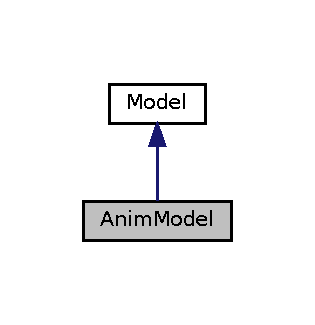
\includegraphics[width=151pt]{classAnimModel__inherit__graph}
\end{center}
\end{figure}


Collaboration diagram for Anim\+Model\+:
\nopagebreak
\begin{figure}[H]
\begin{center}
\leavevmode
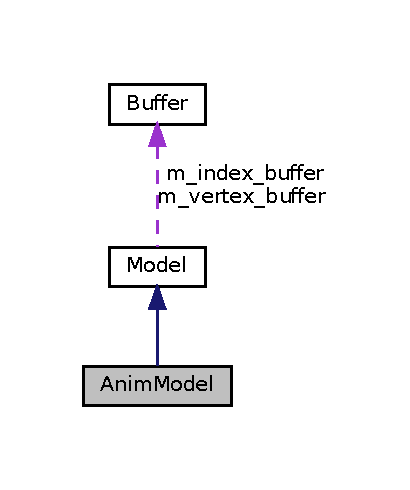
\includegraphics[width=197pt]{classAnimModel__coll__graph}
\end{center}
\end{figure}
\subsection*{Public Member Functions}
\begin{DoxyCompactItemize}
\item 
\mbox{\Hypertarget{classAnimModel_a7d7da460f196334227d35a273069699f}\label{classAnimModel_a7d7da460f196334227d35a273069699f}} 
void {\bfseries Resize\+Bone\+Data\+List} ()
\item 
\mbox{\Hypertarget{classAnimModel_a13cb24e2748e157a5a7365b3c4ec103a}\label{classAnimModel_a13cb24e2748e157a5a7365b3c4ec103a}} 
void {\bfseries Pass\+Indices\+And\+Weights\+Per\+Mesh} (std\+::vector$<$ std\+::vector$<$ int $>$$>$ const \&indices, std\+::vector$<$ std\+::vector$<$ float $>$$>$ const \&weights)
\end{DoxyCompactItemize}
\subsection*{Public Attributes}
\begin{DoxyCompactItemize}
\item 
\mbox{\Hypertarget{classAnimModel_aceed3b69ed40893d926333b1843e837e}\label{classAnimModel_aceed3b69ed40893d926333b1843e837e}} 
std\+::unordered\+\_\+map$<$ std\+::string, \hyperlink{structBone}{Bone} $>$ \hyperlink{classAnimModel_aceed3b69ed40893d926333b1843e837e}{bone\+Map}
\begin{DoxyCompactList}\small\item\em Contains the list of bone with their name. \end{DoxyCompactList}\end{DoxyCompactItemize}
\subsection*{Additional Inherited Members}


\subsection{Detailed Description}
Define the interface for interacting with Animated \hyperlink{classModel}{Model}. 

The documentation for this class was generated from the following files\+:\begin{DoxyCompactItemize}
\item 
Animation/\hyperlink{AnimModel_8h}{Anim\+Model.\+h}\item 
Animation/Anim\+Model.\+cpp\end{DoxyCompactItemize}

\hypertarget{structAnimState}{}\section{Anim\+State Struct Reference}
\label{structAnimState}\index{Anim\+State@{Anim\+State}}


Collaboration diagram for Anim\+State\+:\nopagebreak
\begin{figure}[H]
\begin{center}
\leavevmode
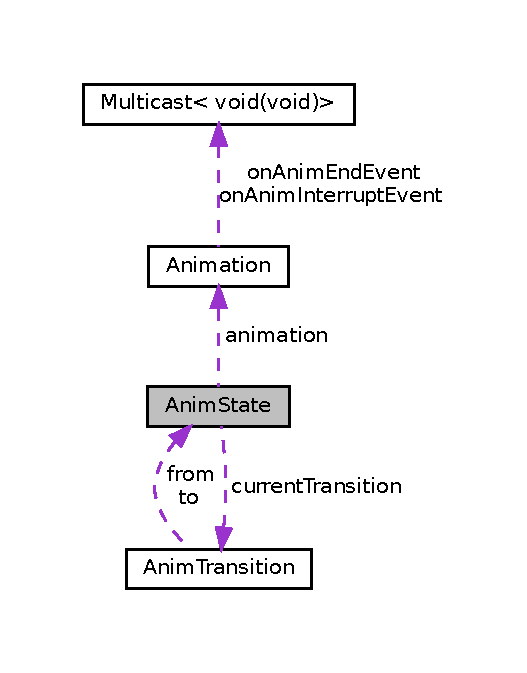
\includegraphics[width=233pt]{structAnimState__coll__graph}
\end{center}
\end{figure}
\subsection*{Public Member Functions}
\begin{DoxyCompactItemize}
\item 
\mbox{\Hypertarget{structAnimState_aade1f3a6b816a8ca9848891d9907a3b0}\label{structAnimState_aade1f3a6b816a8ca9848891d9907a3b0}} 
{\bfseries Anim\+State} (std\+::string name, \hyperlink{structAnimation}{Animation} $\ast$anim)
\item 
\mbox{\Hypertarget{structAnimState_a3f768e0e2231e5ef88cc5c99ba504530}\label{structAnimState_a3f768e0e2231e5ef88cc5c99ba504530}} 
void {\bfseries Set\+Transition} (\hyperlink{structAnimState}{Anim\+State} $\ast$target, float duration, std\+::vector$<$ std\+::string $>$ triggers)
\item 
\mbox{\Hypertarget{structAnimState_a837a54cacb32a66f5b6820c70a1b4087}\label{structAnimState_a837a54cacb32a66f5b6820c70a1b4087}} 
void {\bfseries Check\+All\+Transitions} (std\+::unordered\+\_\+map$<$ std\+::string, int $>$ const \&triggers)
\item 
\mbox{\Hypertarget{structAnimState_aceb8e4d8277433e1963513e09efdfd13}\label{structAnimState_aceb8e4d8277433e1963513e09efdfd13}} 
void {\bfseries Enter\+Transition} (\hyperlink{structAnimTransition}{Anim\+Transition} $\ast$transition)
\item 
\mbox{\Hypertarget{structAnimState_a9cf2327df0e266aa2b0b997cb657e8c7}\label{structAnimState_a9cf2327df0e266aa2b0b997cb657e8c7}} 
void {\bfseries Exit\+Transition} ()
\item 
\mbox{\Hypertarget{structAnimState_aa7ce8cb621dc185ff1b95548b286f6a1}\label{structAnimState_aa7ce8cb621dc185ff1b95548b286f6a1}} 
void {\bfseries Animation\+End\+Handler} ()
\end{DoxyCompactItemize}
\subsection*{Public Attributes}
\begin{DoxyCompactItemize}
\item 
\mbox{\Hypertarget{structAnimState_a3fc2bc133d23f7e11646e98b21a509b7}\label{structAnimState_a3fc2bc133d23f7e11646e98b21a509b7}} 
std\+::string {\bfseries state\+Name}
\item 
\mbox{\Hypertarget{structAnimState_a69e8df8ec31e861fa4313081a0114091}\label{structAnimState_a69e8df8ec31e861fa4313081a0114091}} 
\hyperlink{structAnimation}{Animation} $\ast$ {\bfseries animation}
\item 
\mbox{\Hypertarget{structAnimState_a83742f16bd6f9650fbc493523d8b5b6c}\label{structAnimState_a83742f16bd6f9650fbc493523d8b5b6c}} 
float {\bfseries anim\+Time}
\item 
\mbox{\Hypertarget{structAnimState_a25790df877ce752e839f7f4db199f446}\label{structAnimState_a25790df877ce752e839f7f4db199f446}} 
float {\bfseries speed}
\item 
\mbox{\Hypertarget{structAnimState_a6162838804ebe7bbe208d3affa089308}\label{structAnimState_a6162838804ebe7bbe208d3affa089308}} 
bool {\bfseries is\+Anim\+Running}
\item 
\mbox{\Hypertarget{structAnimState_a8dbd55f6f675b10fe2449df761018e19}\label{structAnimState_a8dbd55f6f675b10fe2449df761018e19}} 
bool {\bfseries is\+In\+Transition}
\item 
\mbox{\Hypertarget{structAnimState_a5836adc57bcbc24a7c43c9021afec4c0}\label{structAnimState_a5836adc57bcbc24a7c43c9021afec4c0}} 
\hyperlink{structAnimTransition}{Anim\+Transition} $\ast$ {\bfseries current\+Transition}
\item 
\mbox{\Hypertarget{structAnimState_a11936add4f5684603ddfd767749128b7}\label{structAnimState_a11936add4f5684603ddfd767749128b7}} 
std\+::vector$<$ \hyperlink{structAnimTransition}{Anim\+Transition} $\ast$ $>$ {\bfseries transitions}
\end{DoxyCompactItemize}


The documentation for this struct was generated from the following file\+:\begin{DoxyCompactItemize}
\item 
Animation/Animator\+Controller.\+h\end{DoxyCompactItemize}

\hypertarget{structAnimTransition}{}\section{Anim\+Transition Struct Reference}
\label{structAnimTransition}\index{Anim\+Transition@{Anim\+Transition}}


Collaboration diagram for Anim\+Transition\+:\nopagebreak
\begin{figure}[H]
\begin{center}
\leavevmode
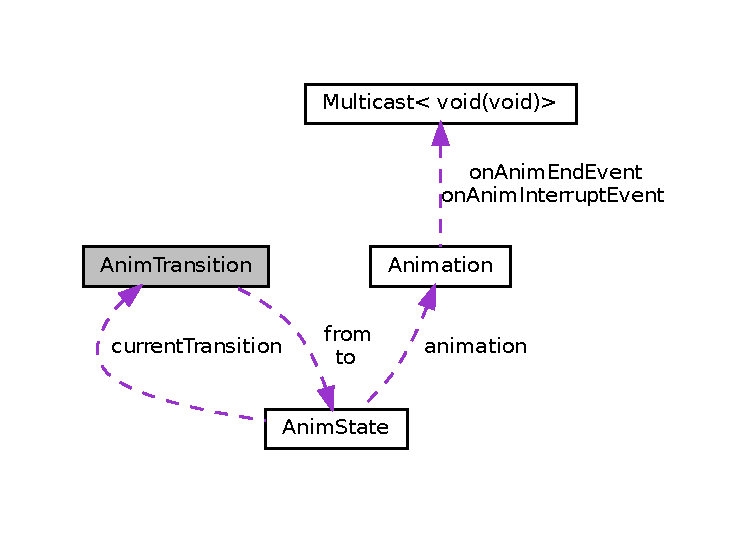
\includegraphics[width=337pt]{structAnimTransition__coll__graph}
\end{center}
\end{figure}
\subsection*{Public Member Functions}
\begin{DoxyCompactItemize}
\item 
\mbox{\Hypertarget{structAnimTransition_adae6a616bfb3af473694a911f6a454f8}\label{structAnimTransition_adae6a616bfb3af473694a911f6a454f8}} 
{\bfseries Anim\+Transition} (\hyperlink{structAnimState}{Anim\+State} $\ast$from, \hyperlink{structAnimState}{Anim\+State} $\ast$to, float dur)
\item 
\mbox{\Hypertarget{structAnimTransition_a3bcab7f4f01efd7ff1fef219353ff7fd}\label{structAnimTransition_a3bcab7f4f01efd7ff1fef219353ff7fd}} 
bool {\bfseries Check\+Condition} (std\+::unordered\+\_\+map$<$ std\+::string, int $>$ const \&triggers)
\end{DoxyCompactItemize}
\subsection*{Public Attributes}
\begin{DoxyCompactItemize}
\item 
\mbox{\Hypertarget{structAnimTransition_a3a3a68577c477a031437d5f246141db7}\label{structAnimTransition_a3a3a68577c477a031437d5f246141db7}} 
\hyperlink{structAnimState}{Anim\+State} $\ast$ {\bfseries from}
\item 
\mbox{\Hypertarget{structAnimTransition_a73bd8f29355ac7b233647d296d9a061e}\label{structAnimTransition_a73bd8f29355ac7b233647d296d9a061e}} 
\hyperlink{structAnimState}{Anim\+State} $\ast$ {\bfseries to}
\item 
\mbox{\Hypertarget{structAnimTransition_acd901f21fdabd3da04664b909b50b7de}\label{structAnimTransition_acd901f21fdabd3da04664b909b50b7de}} 
float {\bfseries transition\+Duration}
\item 
\mbox{\Hypertarget{structAnimTransition_aee7a43acbecd5bb1220a1c478af2732d}\label{structAnimTransition_aee7a43acbecd5bb1220a1c478af2732d}} 
float {\bfseries transition\+Time}
\item 
\mbox{\Hypertarget{structAnimTransition_af3fa828e2da65031824d064e33d1c522}\label{structAnimTransition_af3fa828e2da65031824d064e33d1c522}} 
std\+::vector$<$ \hyperlink{structAnimCondition}{Anim\+Condition} $>$ {\bfseries conditions}
\end{DoxyCompactItemize}


The documentation for this struct was generated from the following file\+:\begin{DoxyCompactItemize}
\item 
Animation/Animator\+Controller.\+h\end{DoxyCompactItemize}

\hypertarget{structAnimVertexData}{}\section{Anim\+Vertex\+Data Struct Reference}
\label{structAnimVertexData}\index{Anim\+Vertex\+Data@{Anim\+Vertex\+Data}}


Define 3D mesh data for animated model with bone hierarchy.  




{\ttfamily \#include $<$Anim\+Model.\+h$>$}



Collaboration diagram for Anim\+Vertex\+Data\+:
\nopagebreak
\begin{figure}[H]
\begin{center}
\leavevmode
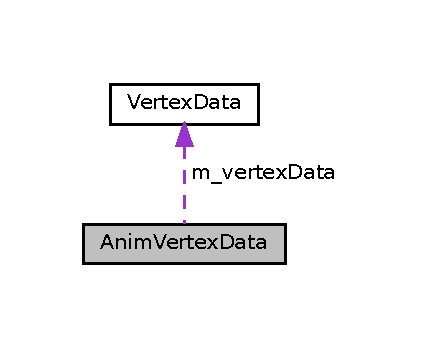
\includegraphics[width=202pt]{structAnimVertexData__coll__graph}
\end{center}
\end{figure}
\subsection*{Public Member Functions}
\begin{DoxyCompactItemize}
\item 
\mbox{\Hypertarget{structAnimVertexData_a1e40cc145ac05a4592808aacf386dac9}\label{structAnimVertexData_a1e40cc145ac05a4592808aacf386dac9}} 
{\bfseries Anim\+Vertex\+Data} (const \hyperlink{structVertexData}{Vertex\+Data} \&vertex\+Data)
\end{DoxyCompactItemize}
\subsection*{Public Attributes}
\begin{DoxyCompactItemize}
\item 
\mbox{\Hypertarget{structAnimVertexData_a128ebc399fe151b2581260866b4be3fd}\label{structAnimVertexData_a128ebc399fe151b2581260866b4be3fd}} 
\hyperlink{structVertexData}{Vertex\+Data} {\bfseries m\+\_\+vertex\+Data}
\item 
\mbox{\Hypertarget{structAnimVertexData_af3182e3c64d06876913bc91e5ddc24ff}\label{structAnimVertexData_af3182e3c64d06876913bc91e5ddc24ff}} 
int32\+\_\+t {\bfseries m\+\_\+bone\+Indices} \mbox{[}4\mbox{]}
\item 
\mbox{\Hypertarget{structAnimVertexData_a2eebb4c79533a02a0cf9c4c2f50e1b2e}\label{structAnimVertexData_a2eebb4c79533a02a0cf9c4c2f50e1b2e}} 
float {\bfseries m\+\_\+bone\+Weights} \mbox{[}4\mbox{]}
\end{DoxyCompactItemize}


\subsection{Detailed Description}
Define 3D mesh data for animated model with bone hierarchy. 

The documentation for this struct was generated from the following file\+:\begin{DoxyCompactItemize}
\item 
Animation/\hyperlink{AnimModel_8h}{Anim\+Model.\+h}\end{DoxyCompactItemize}

\hypertarget{classAppRenderer}{}\section{App\+Renderer Class Reference}
\label{classAppRenderer}\index{App\+Renderer@{App\+Renderer}}


The high level renderer interface.  




{\ttfamily \#include $<$App\+Renderer.\+h$>$}

\subsection*{Public Member Functions}
\begin{DoxyCompactItemize}
\item 
\hyperlink{classAppRenderer_a01b9e6fe7b454466ea00c81d0eb8a89c}{App\+Renderer} (S\+D\+L\+\_\+\+Window \&sdl\+Window, \hyperlink{classResourceManager}{Resource\+Manager} $\ast$resource\+Manager, \hyperlink{classCameraManager}{Camera\+Manager} $\ast$camera\+Manager)
\begin{DoxyCompactList}\small\item\em Construct a new App Renderer object. \end{DoxyCompactList}\item 
void \hyperlink{classAppRenderer_afef47670f4584e2caa6fa750aacd089e}{Update\+App\+Renderer} (float dt)
\begin{DoxyCompactList}\small\item\em Contains update logic for \hyperlink{classAppRenderer}{App\+Renderer}. No render api is called in this function. \end{DoxyCompactList}\item 
\mbox{\Hypertarget{classAppRenderer_a2a094187727c735aeb1ca376f4d02f29}\label{classAppRenderer_a2a094187727c735aeb1ca376f4d02f29}} 
void \hyperlink{classAppRenderer_a2a094187727c735aeb1ca376f4d02f29}{Render\+App} ()
\begin{DoxyCompactList}\small\item\em Render all queued render request info to swap chain. \end{DoxyCompactList}\item 
\mbox{\Hypertarget{classAppRenderer_a393b3c6f865bc07612f26e185100ca6a}\label{classAppRenderer_a393b3c6f865bc07612f26e185100ca6a}} 
void \hyperlink{classAppRenderer_a393b3c6f865bc07612f26e185100ca6a}{Present\+App} ()
\begin{DoxyCompactList}\small\item\em Present rendered data to swapchain. \end{DoxyCompactList}\item 
\mbox{\Hypertarget{classAppRenderer_ab0d289c6d6375e274c91f42d3256d584}\label{classAppRenderer_ab0d289c6d6375e274c91f42d3256d584}} 
void \hyperlink{classAppRenderer_ab0d289c6d6375e274c91f42d3256d584}{Release} ()
\begin{DoxyCompactList}\small\item\em Release all graphics related resources. \end{DoxyCompactList}\item 
\hyperlink{classDXRenderer}{D\+X\+Renderer} $\ast$ \hyperlink{classAppRenderer_a22dc8c3e1972281376b321336d6451a3}{Get\+D\+X\+Renderer} ()
\begin{DoxyCompactList}\small\item\em Get \hyperlink{classDXRenderer}{D\+X\+Renderer}, a D3\+D11 interface renderer. \end{DoxyCompactList}\item 
S\+D\+L\+\_\+\+Window \& \hyperlink{classAppRenderer_ae523d428966c527b385a65bae7bdb086}{Get\+S\+D\+L\+Window} ()
\begin{DoxyCompactList}\small\item\em Get reference to S\+D\+L\+Window. \end{DoxyCompactList}\item 
\hyperlink{classDebugRendering}{Debug\+Rendering} \& \hyperlink{classAppRenderer_af4f38db33ff5ff4a321e9c44e9472b41}{Get\+Debug\+Rendering} ()
\begin{DoxyCompactList}\small\item\em Get the Debug Rendering object. \end{DoxyCompactList}\item 
\hyperlink{classParticleRendering}{Particle\+Rendering} \& \hyperlink{classAppRenderer_a0e5afe33f9a99df3c7b546710d20aa45}{Get\+Particle\+Rendering} ()
\begin{DoxyCompactList}\small\item\em Get the \hyperlink{structParticle}{Particle} Rendering object. \end{DoxyCompactList}\item 
void \hyperlink{classAppRenderer_af7ca20884c77f5d17a59835742611803}{Register\+Basic\+Instance} (const \hyperlink{structInstanceRenderData}{Instance\+Render\+Data} \&instance\+Render\+Data)
\begin{DoxyCompactList}\small\item\em Pass render info request for any primitive meshes or artist defined meshes. \end{DoxyCompactList}\item 
void \hyperlink{classAppRenderer_ab12a770688fb1d142c6701acebfdd6b4}{Register\+Directional\+Light\+Instance} (const \hyperlink{structDirectionalLightInstanceData}{Directional\+Light\+Instance\+Data} \&directional\+Light\+Instance\+Data)
\begin{DoxyCompactList}\small\item\em Pass directional lighting info to the current scene. Used to illuminate scene globally. \end{DoxyCompactList}\item 
void \hyperlink{classAppRenderer_a8dcf762bbcbdce2de5e3f0a8810ab5dc}{Register\+Halo\+Effect\+Instance} (const \hyperlink{structHaloEffectInstanceData}{Halo\+Effect\+Instance\+Data} \&halo\+Effect\+Data)
\begin{DoxyCompactList}\small\item\em Pass halo effect info to the current scene. Sphere-\/like glow effect. \end{DoxyCompactList}\item 
void \hyperlink{classAppRenderer_a214f01562badba6e4f10038a239917f8}{Register\+Point\+Light\+Instance} (const \hyperlink{structPointLightInstanceData}{Point\+Light\+Instance\+Data} \&point\+Light\+Instance\+Data)
\begin{DoxyCompactList}\small\item\em Pass point lighting info to the current scene. Used to illuminate portion of the scene. \end{DoxyCompactList}\item 
void \hyperlink{classAppRenderer_a28300e8e65298f09dff5d469dea3f85c}{Register\+Bone\+Mesh\+Instance} (const \hyperlink{structBoneMeshInstanceRenderData}{Bone\+Mesh\+Instance\+Render\+Data} \&bone\+Mesh\+Instance\+Data)
\begin{DoxyCompactList}\small\item\em Pass render info request for animated skinned model. \end{DoxyCompactList}\item 
void \hyperlink{classAppRenderer_ac80c3259382af5a0bd7163132da9c718}{Register\+U\+I\+Object\+Instance} (const \hyperlink{structUIObjectInstanceRenderData}{U\+I\+Object\+Instance\+Render\+Data} \&ui\+Object\+Instance\+Data)
\begin{DoxyCompactList}\small\item\em Pass render info request for orthographic UI rendering. \end{DoxyCompactList}\item 
void \hyperlink{classAppRenderer_aaca975e8c6b1ac11095591926d942e4c}{Register\+Text\+Font\+Instance} (const \hyperlink{structTextFontInstanceRenderData}{Text\+Font\+Instance\+Render\+Data} \&text\+Font\+Instance\+Data)
\begin{DoxyCompactList}\small\item\em Pass render info request for D\+X11 screen space text rendering. \end{DoxyCompactList}\item 
void \hyperlink{classAppRenderer_a9d8be5bfc486bd5bf432366784477ecf}{Register\+Text\+Font\+Instance} (const std\+::string \&text, uint32\+\_\+t font\+Type, const Vector2 \&position, const Vector3 \&color, const Vector3 \&scale, float rotation)
\begin{DoxyCompactList}\small\item\em Pass render info request for D\+X11 screen space text rendering. \end{DoxyCompactList}\item 
void \hyperlink{classAppRenderer_ab636c593d1bb6b85dae508ee2945c9a8}{Register\+Text\+Font\+Instance} (const std\+::wstring \&text, Font\+Type font\+Type, const Vector2 \&position, const Vector3 \&color, const Vector3 \&scale, float rotation)
\begin{DoxyCompactList}\small\item\em Pass render info request for D\+X11 screen space text rendering. \end{DoxyCompactList}\item 
void \hyperlink{classAppRenderer_a46cea9dbc355592e2b3d74b8ef297175}{Register\+Process\+Skybox\+Irradiance\+Instance} (const \hyperlink{structProcessSkyboxIrradianceInstanceData}{Process\+Skybox\+Irradiance\+Instance\+Data} \&process\+Instance\+Data)
\begin{DoxyCompactList}\small\item\em Pass unbaked skybox data to the internal app renderer. App rendere bake the skybox to irradiance \& specular data. \end{DoxyCompactList}\item 
void \hyperlink{classAppRenderer_a596152f75036dfc597666d3ead6e0959}{Register\+Baked\+Skybox\+Irradiance\+Instance} (const \hyperlink{structBakedSkyboxIrradianceInstanceData}{Baked\+Skybox\+Irradiance\+Instance\+Data} \&baked\+Instance\+Data)
\begin{DoxyCompactList}\small\item\em Pass baked skybox irradiance data to the scene. Will illuminate the scene globally based on skybox H\+DR illumination. \end{DoxyCompactList}\item 
\mbox{\Hypertarget{classAppRenderer_abcb06ec3a4f44df9a6b93c9da882e150}\label{classAppRenderer_abcb06ec3a4f44df9a6b93c9da882e150}} 
void \hyperlink{classAppRenderer_abcb06ec3a4f44df9a6b93c9da882e150}{Initialize\+Renderer} ()
\begin{DoxyCompactList}\small\item\em Initialize D\+X11 renderer. \end{DoxyCompactList}\item 
\mbox{\Hypertarget{classAppRenderer_a469d6a18301eabc3c4942a2a7d95a5fe}\label{classAppRenderer_a469d6a18301eabc3c4942a2a7d95a5fe}} 
void \hyperlink{classAppRenderer_a469d6a18301eabc3c4942a2a7d95a5fe}{Initialize\+Resources} ()
\begin{DoxyCompactList}\small\item\em Initialize high level resources. \end{DoxyCompactList}\item 
\mbox{\Hypertarget{classAppRenderer_a243e0f5390b30ead7661cda98fd606a6}\label{classAppRenderer_a243e0f5390b30ead7661cda98fd606a6}} 
void \hyperlink{classAppRenderer_a243e0f5390b30ead7661cda98fd606a6}{Load\+Content} ()
\begin{DoxyCompactList}\small\item\em Load high level resources (this is set to be called for every windows resize event in the future) \end{DoxyCompactList}\item 
\hyperlink{classMomentShadowMapRendering}{Moment\+Shadow\+Map\+Rendering} \& \hyperlink{classAppRenderer_af86218b9be6d10b9a5f39e89dc828d53}{Get\+Moment\+Shadow\+Map} ()
\begin{DoxyCompactList}\small\item\em Get the Moment Shadow Map Rendering object. \end{DoxyCompactList}\end{DoxyCompactItemize}
\subsection*{Friends}
\begin{DoxyCompactItemize}
\item 
\mbox{\Hypertarget{classAppRenderer_a355bf32616f2e1751ee46bd315e905e5}\label{classAppRenderer_a355bf32616f2e1751ee46bd315e905e5}} 
class {\bfseries Deferred\+Rendering}
\item 
\mbox{\Hypertarget{classAppRenderer_a6611940d699c1a465f439495d9ad98d3}\label{classAppRenderer_a6611940d699c1a465f439495d9ad98d3}} 
class {\bfseries Debug\+Rendering}
\item 
\mbox{\Hypertarget{classAppRenderer_ad456619a35eac3a6efbe8557a0ccc425}\label{classAppRenderer_ad456619a35eac3a6efbe8557a0ccc425}} 
class {\bfseries Depth\+Pass\+Rendering}
\item 
\mbox{\Hypertarget{classAppRenderer_a23797ad96fd0436c2365d4c86df7adde}\label{classAppRenderer_a23797ad96fd0436c2365d4c86df7adde}} 
class {\bfseries Moment\+Shadow\+Map\+Rendering}
\item 
\mbox{\Hypertarget{classAppRenderer_ac54ffcb054b1f5a95256118dbdeae9f2}\label{classAppRenderer_ac54ffcb054b1f5a95256118dbdeae9f2}} 
class {\bfseries M\+S\+A\+A\+Resolve\+Pass}
\item 
\mbox{\Hypertarget{classAppRenderer_a0cb4dedb676c1c060cf82ddb22f668bf}\label{classAppRenderer_a0cb4dedb676c1c060cf82ddb22f668bf}} 
class {\bfseries Particle\+Rendering}
\item 
\mbox{\Hypertarget{classAppRenderer_a7bec99218ac38952a4baa8888bc7fedc}\label{classAppRenderer_a7bec99218ac38952a4baa8888bc7fedc}} 
class {\bfseries Deferred\+Rendering\+Instance}
\item 
\mbox{\Hypertarget{classAppRenderer_aa2fce3a4ae64b69f01e0fd64ba26023a}\label{classAppRenderer_aa2fce3a4ae64b69f01e0fd64ba26023a}} 
class {\bfseries Debug\+Rendering\+Instance}
\item 
\mbox{\Hypertarget{classAppRenderer_aba9f3240241811e775ef4280a9df4333}\label{classAppRenderer_aba9f3240241811e775ef4280a9df4333}} 
class {\bfseries Particle\+Rendering\+Instance}
\item 
\mbox{\Hypertarget{classAppRenderer_a0afda4cbff6d9e5529eca6ee18a2a129}\label{classAppRenderer_a0afda4cbff6d9e5529eca6ee18a2a129}} 
class {\bfseries App\+Renderer\+Instance}
\item 
\mbox{\Hypertarget{classAppRenderer_a1b9897dd2ae9e6c35d99de6c02d2b693}\label{classAppRenderer_a1b9897dd2ae9e6c35d99de6c02d2b693}} 
class {\bfseries Equirectangular\+To\+Skybox\+Render}
\item 
\mbox{\Hypertarget{classAppRenderer_a2ed53da06aa8c96971b58644b85ea2d3}\label{classAppRenderer_a2ed53da06aa8c96971b58644b85ea2d3}} 
class {\bfseries Equirectangular\+To\+Skybox\+Render\+Instance}
\item 
\mbox{\Hypertarget{classAppRenderer_afeb3653020f8cc65d4b08c7ea9559a43}\label{classAppRenderer_afeb3653020f8cc65d4b08c7ea9559a43}} 
class {\bfseries I\+B\+L\+Filter\+Env\+Map\+Pass}
\item 
\mbox{\Hypertarget{classAppRenderer_a931e3cacb3eb1341332fd7477decd15d}\label{classAppRenderer_a931e3cacb3eb1341332fd7477decd15d}} 
class {\bfseries U\+I\+Object\+Rendering}
\item 
\mbox{\Hypertarget{classAppRenderer_af8087aef5ebe8f9a42bfabe1e0672728}\label{classAppRenderer_af8087aef5ebe8f9a42bfabe1e0672728}} 
class {\bfseries U\+I\+Object\+Rendering\+Instance}
\item 
\mbox{\Hypertarget{classAppRenderer_a4708d497b34a7f0c5e0a38cfa536a26c}\label{classAppRenderer_a4708d497b34a7f0c5e0a38cfa536a26c}} 
class {\bfseries Text\+Rendering}
\item 
\mbox{\Hypertarget{classAppRenderer_a5532c3b535b4f2a814054dba701936df}\label{classAppRenderer_a5532c3b535b4f2a814054dba701936df}} 
class {\bfseries Text\+Rendering\+Instance}
\end{DoxyCompactItemize}


\subsection{Detailed Description}
The high level renderer interface. 

\subsection{Constructor \& Destructor Documentation}
\mbox{\Hypertarget{classAppRenderer_a01b9e6fe7b454466ea00c81d0eb8a89c}\label{classAppRenderer_a01b9e6fe7b454466ea00c81d0eb8a89c}} 
\index{App\+Renderer@{App\+Renderer}!App\+Renderer@{App\+Renderer}}
\index{App\+Renderer@{App\+Renderer}!App\+Renderer@{App\+Renderer}}
\subsubsection{\texorpdfstring{App\+Renderer()}{AppRenderer()}}
{\footnotesize\ttfamily App\+Renderer\+::\+App\+Renderer (\begin{DoxyParamCaption}\item[{S\+D\+L\+\_\+\+Window \&}]{sdl\+Window,  }\item[{\hyperlink{classResourceManager}{Resource\+Manager} $\ast$}]{resource\+Manager,  }\item[{\hyperlink{classCameraManager}{Camera\+Manager} $\ast$}]{camera\+Manager }\end{DoxyParamCaption})}



Construct a new App Renderer object. 


\begin{DoxyParams}{Parameters}
{\em sdl\+Window} & \\
\hline
{\em resource\+Manager} & \\
\hline
{\em camera\+Manager} & \\
\hline
\end{DoxyParams}


\subsection{Member Function Documentation}
\mbox{\Hypertarget{classAppRenderer_af4f38db33ff5ff4a321e9c44e9472b41}\label{classAppRenderer_af4f38db33ff5ff4a321e9c44e9472b41}} 
\index{App\+Renderer@{App\+Renderer}!Get\+Debug\+Rendering@{Get\+Debug\+Rendering}}
\index{Get\+Debug\+Rendering@{Get\+Debug\+Rendering}!App\+Renderer@{App\+Renderer}}
\subsubsection{\texorpdfstring{Get\+Debug\+Rendering()}{GetDebugRendering()}}
{\footnotesize\ttfamily \hyperlink{classDebugRendering}{Debug\+Rendering} \& App\+Renderer\+::\+Get\+Debug\+Rendering (\begin{DoxyParamCaption}{ }\end{DoxyParamCaption})}



Get the Debug Rendering object. 

\begin{DoxyReturn}{Returns}
\hyperlink{classDebugRendering}{Debug\+Rendering}\& 
\end{DoxyReturn}
\mbox{\Hypertarget{classAppRenderer_a22dc8c3e1972281376b321336d6451a3}\label{classAppRenderer_a22dc8c3e1972281376b321336d6451a3}} 
\index{App\+Renderer@{App\+Renderer}!Get\+D\+X\+Renderer@{Get\+D\+X\+Renderer}}
\index{Get\+D\+X\+Renderer@{Get\+D\+X\+Renderer}!App\+Renderer@{App\+Renderer}}
\subsubsection{\texorpdfstring{Get\+D\+X\+Renderer()}{GetDXRenderer()}}
{\footnotesize\ttfamily \hyperlink{classDXRenderer}{D\+X\+Renderer} $\ast$ App\+Renderer\+::\+Get\+D\+X\+Renderer (\begin{DoxyParamCaption}{ }\end{DoxyParamCaption})}



Get \hyperlink{classDXRenderer}{D\+X\+Renderer}, a D3\+D11 interface renderer. 

\begin{DoxyReturn}{Returns}
D\+X\+Renderer$\ast$ 
\end{DoxyReturn}
\mbox{\Hypertarget{classAppRenderer_af86218b9be6d10b9a5f39e89dc828d53}\label{classAppRenderer_af86218b9be6d10b9a5f39e89dc828d53}} 
\index{App\+Renderer@{App\+Renderer}!Get\+Moment\+Shadow\+Map@{Get\+Moment\+Shadow\+Map}}
\index{Get\+Moment\+Shadow\+Map@{Get\+Moment\+Shadow\+Map}!App\+Renderer@{App\+Renderer}}
\subsubsection{\texorpdfstring{Get\+Moment\+Shadow\+Map()}{GetMomentShadowMap()}}
{\footnotesize\ttfamily \hyperlink{classMomentShadowMapRendering}{Moment\+Shadow\+Map\+Rendering} \& App\+Renderer\+::\+Get\+Moment\+Shadow\+Map (\begin{DoxyParamCaption}{ }\end{DoxyParamCaption})}



Get the Moment Shadow Map Rendering object. 

\begin{DoxyReturn}{Returns}
\hyperlink{classMomentShadowMapRendering}{Moment\+Shadow\+Map\+Rendering}\& 
\end{DoxyReturn}
\mbox{\Hypertarget{classAppRenderer_a0e5afe33f9a99df3c7b546710d20aa45}\label{classAppRenderer_a0e5afe33f9a99df3c7b546710d20aa45}} 
\index{App\+Renderer@{App\+Renderer}!Get\+Particle\+Rendering@{Get\+Particle\+Rendering}}
\index{Get\+Particle\+Rendering@{Get\+Particle\+Rendering}!App\+Renderer@{App\+Renderer}}
\subsubsection{\texorpdfstring{Get\+Particle\+Rendering()}{GetParticleRendering()}}
{\footnotesize\ttfamily \hyperlink{classParticleRendering}{Particle\+Rendering} \& App\+Renderer\+::\+Get\+Particle\+Rendering (\begin{DoxyParamCaption}{ }\end{DoxyParamCaption})}



Get the \hyperlink{structParticle}{Particle} Rendering object. 

\begin{DoxyReturn}{Returns}
\hyperlink{classParticleRendering}{Particle\+Rendering}\& 
\end{DoxyReturn}
\mbox{\Hypertarget{classAppRenderer_ae523d428966c527b385a65bae7bdb086}\label{classAppRenderer_ae523d428966c527b385a65bae7bdb086}} 
\index{App\+Renderer@{App\+Renderer}!Get\+S\+D\+L\+Window@{Get\+S\+D\+L\+Window}}
\index{Get\+S\+D\+L\+Window@{Get\+S\+D\+L\+Window}!App\+Renderer@{App\+Renderer}}
\subsubsection{\texorpdfstring{Get\+S\+D\+L\+Window()}{GetSDLWindow()}}
{\footnotesize\ttfamily S\+D\+L\+\_\+\+Window \& App\+Renderer\+::\+Get\+S\+D\+L\+Window (\begin{DoxyParamCaption}{ }\end{DoxyParamCaption})}



Get reference to S\+D\+L\+Window. 

\begin{DoxyReturn}{Returns}
S\+D\+L\+\_\+\+Window\& 
\end{DoxyReturn}
\mbox{\Hypertarget{classAppRenderer_a596152f75036dfc597666d3ead6e0959}\label{classAppRenderer_a596152f75036dfc597666d3ead6e0959}} 
\index{App\+Renderer@{App\+Renderer}!Register\+Baked\+Skybox\+Irradiance\+Instance@{Register\+Baked\+Skybox\+Irradiance\+Instance}}
\index{Register\+Baked\+Skybox\+Irradiance\+Instance@{Register\+Baked\+Skybox\+Irradiance\+Instance}!App\+Renderer@{App\+Renderer}}
\subsubsection{\texorpdfstring{Register\+Baked\+Skybox\+Irradiance\+Instance()}{RegisterBakedSkyboxIrradianceInstance()}}
{\footnotesize\ttfamily void App\+Renderer\+::\+Register\+Baked\+Skybox\+Irradiance\+Instance (\begin{DoxyParamCaption}\item[{const \hyperlink{structBakedSkyboxIrradianceInstanceData}{Baked\+Skybox\+Irradiance\+Instance\+Data} \&}]{baked\+Instance\+Data }\end{DoxyParamCaption})}



Pass baked skybox irradiance data to the scene. Will illuminate the scene globally based on skybox H\+DR illumination. 


\begin{DoxyParams}{Parameters}
{\em baked\+Instance\+Data} & \\
\hline
\end{DoxyParams}
\mbox{\Hypertarget{classAppRenderer_af7ca20884c77f5d17a59835742611803}\label{classAppRenderer_af7ca20884c77f5d17a59835742611803}} 
\index{App\+Renderer@{App\+Renderer}!Register\+Basic\+Instance@{Register\+Basic\+Instance}}
\index{Register\+Basic\+Instance@{Register\+Basic\+Instance}!App\+Renderer@{App\+Renderer}}
\subsubsection{\texorpdfstring{Register\+Basic\+Instance()}{RegisterBasicInstance()}}
{\footnotesize\ttfamily void App\+Renderer\+::\+Register\+Basic\+Instance (\begin{DoxyParamCaption}\item[{const \hyperlink{structInstanceRenderData}{Instance\+Render\+Data} \&}]{instance\+Render\+Data }\end{DoxyParamCaption})}



Pass render info request for any primitive meshes or artist defined meshes. 


\begin{DoxyParams}{Parameters}
{\em instance\+Render\+Data} & \\
\hline
\end{DoxyParams}
\mbox{\Hypertarget{classAppRenderer_a28300e8e65298f09dff5d469dea3f85c}\label{classAppRenderer_a28300e8e65298f09dff5d469dea3f85c}} 
\index{App\+Renderer@{App\+Renderer}!Register\+Bone\+Mesh\+Instance@{Register\+Bone\+Mesh\+Instance}}
\index{Register\+Bone\+Mesh\+Instance@{Register\+Bone\+Mesh\+Instance}!App\+Renderer@{App\+Renderer}}
\subsubsection{\texorpdfstring{Register\+Bone\+Mesh\+Instance()}{RegisterBoneMeshInstance()}}
{\footnotesize\ttfamily void App\+Renderer\+::\+Register\+Bone\+Mesh\+Instance (\begin{DoxyParamCaption}\item[{const \hyperlink{structBoneMeshInstanceRenderData}{Bone\+Mesh\+Instance\+Render\+Data} \&}]{bone\+Mesh\+Instance\+Data }\end{DoxyParamCaption})}



Pass render info request for animated skinned model. 


\begin{DoxyParams}{Parameters}
{\em bone\+Mesh\+Instance\+Data} & \\
\hline
\end{DoxyParams}
\mbox{\Hypertarget{classAppRenderer_ab12a770688fb1d142c6701acebfdd6b4}\label{classAppRenderer_ab12a770688fb1d142c6701acebfdd6b4}} 
\index{App\+Renderer@{App\+Renderer}!Register\+Directional\+Light\+Instance@{Register\+Directional\+Light\+Instance}}
\index{Register\+Directional\+Light\+Instance@{Register\+Directional\+Light\+Instance}!App\+Renderer@{App\+Renderer}}
\subsubsection{\texorpdfstring{Register\+Directional\+Light\+Instance()}{RegisterDirectionalLightInstance()}}
{\footnotesize\ttfamily void App\+Renderer\+::\+Register\+Directional\+Light\+Instance (\begin{DoxyParamCaption}\item[{const \hyperlink{structDirectionalLightInstanceData}{Directional\+Light\+Instance\+Data} \&}]{directional\+Light\+Instance\+Data }\end{DoxyParamCaption})}



Pass directional lighting info to the current scene. Used to illuminate scene globally. 


\begin{DoxyParams}{Parameters}
{\em directional\+Light\+Instance\+Data} & \\
\hline
\end{DoxyParams}
\mbox{\Hypertarget{classAppRenderer_a8dcf762bbcbdce2de5e3f0a8810ab5dc}\label{classAppRenderer_a8dcf762bbcbdce2de5e3f0a8810ab5dc}} 
\index{App\+Renderer@{App\+Renderer}!Register\+Halo\+Effect\+Instance@{Register\+Halo\+Effect\+Instance}}
\index{Register\+Halo\+Effect\+Instance@{Register\+Halo\+Effect\+Instance}!App\+Renderer@{App\+Renderer}}
\subsubsection{\texorpdfstring{Register\+Halo\+Effect\+Instance()}{RegisterHaloEffectInstance()}}
{\footnotesize\ttfamily void App\+Renderer\+::\+Register\+Halo\+Effect\+Instance (\begin{DoxyParamCaption}\item[{const \hyperlink{structHaloEffectInstanceData}{Halo\+Effect\+Instance\+Data} \&}]{halo\+Effect\+Data }\end{DoxyParamCaption})}



Pass halo effect info to the current scene. Sphere-\/like glow effect. 


\begin{DoxyParams}{Parameters}
{\em halo\+Effect\+Data} & \\
\hline
\end{DoxyParams}
\mbox{\Hypertarget{classAppRenderer_a214f01562badba6e4f10038a239917f8}\label{classAppRenderer_a214f01562badba6e4f10038a239917f8}} 
\index{App\+Renderer@{App\+Renderer}!Register\+Point\+Light\+Instance@{Register\+Point\+Light\+Instance}}
\index{Register\+Point\+Light\+Instance@{Register\+Point\+Light\+Instance}!App\+Renderer@{App\+Renderer}}
\subsubsection{\texorpdfstring{Register\+Point\+Light\+Instance()}{RegisterPointLightInstance()}}
{\footnotesize\ttfamily void App\+Renderer\+::\+Register\+Point\+Light\+Instance (\begin{DoxyParamCaption}\item[{const \hyperlink{structPointLightInstanceData}{Point\+Light\+Instance\+Data} \&}]{point\+Light\+Instance\+Data }\end{DoxyParamCaption})}



Pass point lighting info to the current scene. Used to illuminate portion of the scene. 


\begin{DoxyParams}{Parameters}
{\em point\+Light\+Instance\+Data} & \\
\hline
\end{DoxyParams}
\mbox{\Hypertarget{classAppRenderer_a46cea9dbc355592e2b3d74b8ef297175}\label{classAppRenderer_a46cea9dbc355592e2b3d74b8ef297175}} 
\index{App\+Renderer@{App\+Renderer}!Register\+Process\+Skybox\+Irradiance\+Instance@{Register\+Process\+Skybox\+Irradiance\+Instance}}
\index{Register\+Process\+Skybox\+Irradiance\+Instance@{Register\+Process\+Skybox\+Irradiance\+Instance}!App\+Renderer@{App\+Renderer}}
\subsubsection{\texorpdfstring{Register\+Process\+Skybox\+Irradiance\+Instance()}{RegisterProcessSkyboxIrradianceInstance()}}
{\footnotesize\ttfamily void App\+Renderer\+::\+Register\+Process\+Skybox\+Irradiance\+Instance (\begin{DoxyParamCaption}\item[{const \hyperlink{structProcessSkyboxIrradianceInstanceData}{Process\+Skybox\+Irradiance\+Instance\+Data} \&}]{process\+Instance\+Data }\end{DoxyParamCaption})}



Pass unbaked skybox data to the internal app renderer. App rendere bake the skybox to irradiance \& specular data. 


\begin{DoxyParams}{Parameters}
{\em process\+Instance\+Data} & \\
\hline
\end{DoxyParams}
\mbox{\Hypertarget{classAppRenderer_aaca975e8c6b1ac11095591926d942e4c}\label{classAppRenderer_aaca975e8c6b1ac11095591926d942e4c}} 
\index{App\+Renderer@{App\+Renderer}!Register\+Text\+Font\+Instance@{Register\+Text\+Font\+Instance}}
\index{Register\+Text\+Font\+Instance@{Register\+Text\+Font\+Instance}!App\+Renderer@{App\+Renderer}}
\subsubsection{\texorpdfstring{Register\+Text\+Font\+Instance()}{RegisterTextFontInstance()}\hspace{0.1cm}{\footnotesize\ttfamily [1/3]}}
{\footnotesize\ttfamily void App\+Renderer\+::\+Register\+Text\+Font\+Instance (\begin{DoxyParamCaption}\item[{const \hyperlink{structTextFontInstanceRenderData}{Text\+Font\+Instance\+Render\+Data} \&}]{text\+Font\+Instance\+Data }\end{DoxyParamCaption})}



Pass render info request for D\+X11 screen space text rendering. 


\begin{DoxyParams}{Parameters}
{\em text\+Font\+Instance\+Data} & \\
\hline
\end{DoxyParams}
\mbox{\Hypertarget{classAppRenderer_a9d8be5bfc486bd5bf432366784477ecf}\label{classAppRenderer_a9d8be5bfc486bd5bf432366784477ecf}} 
\index{App\+Renderer@{App\+Renderer}!Register\+Text\+Font\+Instance@{Register\+Text\+Font\+Instance}}
\index{Register\+Text\+Font\+Instance@{Register\+Text\+Font\+Instance}!App\+Renderer@{App\+Renderer}}
\subsubsection{\texorpdfstring{Register\+Text\+Font\+Instance()}{RegisterTextFontInstance()}\hspace{0.1cm}{\footnotesize\ttfamily [2/3]}}
{\footnotesize\ttfamily void App\+Renderer\+::\+Register\+Text\+Font\+Instance (\begin{DoxyParamCaption}\item[{const std\+::string \&}]{text,  }\item[{uint32\+\_\+t}]{font\+Type,  }\item[{const Vector2 \&}]{position,  }\item[{const Vector3 \&}]{color,  }\item[{const Vector3 \&}]{scale,  }\item[{float}]{rotation }\end{DoxyParamCaption})}



Pass render info request for D\+X11 screen space text rendering. 


\begin{DoxyParams}{Parameters}
{\em text} & \\
\hline
{\em font\+Type} & \\
\hline
{\em position} & \\
\hline
{\em color} & \\
\hline
{\em scale} & \\
\hline
{\em rotation} & \\
\hline
\end{DoxyParams}
\mbox{\Hypertarget{classAppRenderer_ab636c593d1bb6b85dae508ee2945c9a8}\label{classAppRenderer_ab636c593d1bb6b85dae508ee2945c9a8}} 
\index{App\+Renderer@{App\+Renderer}!Register\+Text\+Font\+Instance@{Register\+Text\+Font\+Instance}}
\index{Register\+Text\+Font\+Instance@{Register\+Text\+Font\+Instance}!App\+Renderer@{App\+Renderer}}
\subsubsection{\texorpdfstring{Register\+Text\+Font\+Instance()}{RegisterTextFontInstance()}\hspace{0.1cm}{\footnotesize\ttfamily [3/3]}}
{\footnotesize\ttfamily void App\+Renderer\+::\+Register\+Text\+Font\+Instance (\begin{DoxyParamCaption}\item[{const std\+::wstring \&}]{text,  }\item[{Font\+Type}]{font\+Type,  }\item[{const Vector2 \&}]{position,  }\item[{const Vector3 \&}]{color,  }\item[{const Vector3 \&}]{scale,  }\item[{float}]{rotation }\end{DoxyParamCaption})}



Pass render info request for D\+X11 screen space text rendering. 


\begin{DoxyParams}{Parameters}
{\em text} & \\
\hline
{\em font\+Type} & \\
\hline
{\em position} & \\
\hline
{\em color} & \\
\hline
{\em scale} & \\
\hline
{\em rotation} & \\
\hline
\end{DoxyParams}
\mbox{\Hypertarget{classAppRenderer_ac80c3259382af5a0bd7163132da9c718}\label{classAppRenderer_ac80c3259382af5a0bd7163132da9c718}} 
\index{App\+Renderer@{App\+Renderer}!Register\+U\+I\+Object\+Instance@{Register\+U\+I\+Object\+Instance}}
\index{Register\+U\+I\+Object\+Instance@{Register\+U\+I\+Object\+Instance}!App\+Renderer@{App\+Renderer}}
\subsubsection{\texorpdfstring{Register\+U\+I\+Object\+Instance()}{RegisterUIObjectInstance()}}
{\footnotesize\ttfamily void App\+Renderer\+::\+Register\+U\+I\+Object\+Instance (\begin{DoxyParamCaption}\item[{const \hyperlink{structUIObjectInstanceRenderData}{U\+I\+Object\+Instance\+Render\+Data} \&}]{ui\+Object\+Instance\+Data }\end{DoxyParamCaption})}



Pass render info request for orthographic UI rendering. 


\begin{DoxyParams}{Parameters}
{\em ui\+Object\+Instance\+Data} & \\
\hline
\end{DoxyParams}
\mbox{\Hypertarget{classAppRenderer_afef47670f4584e2caa6fa750aacd089e}\label{classAppRenderer_afef47670f4584e2caa6fa750aacd089e}} 
\index{App\+Renderer@{App\+Renderer}!Update\+App\+Renderer@{Update\+App\+Renderer}}
\index{Update\+App\+Renderer@{Update\+App\+Renderer}!App\+Renderer@{App\+Renderer}}
\subsubsection{\texorpdfstring{Update\+App\+Renderer()}{UpdateAppRenderer()}}
{\footnotesize\ttfamily void App\+Renderer\+::\+Update\+App\+Renderer (\begin{DoxyParamCaption}\item[{float}]{dt }\end{DoxyParamCaption})}



Contains update logic for \hyperlink{classAppRenderer}{App\+Renderer}. No render api is called in this function. 


\begin{DoxyParams}{Parameters}
{\em dt} & \\
\hline
\end{DoxyParams}


The documentation for this class was generated from the following files\+:\begin{DoxyCompactItemize}
\item 
Graphics/\hyperlink{AppRenderer_8h}{App\+Renderer.\+h}\item 
Graphics/App\+Renderer.\+cpp\end{DoxyCompactItemize}

\hypertarget{structAppRendererContext}{}\section{App\+Renderer\+Context Struct Reference}
\label{structAppRendererContext}\index{App\+Renderer\+Context@{App\+Renderer\+Context}}


Collaboration diagram for App\+Renderer\+Context\+:
\nopagebreak
\begin{figure}[H]
\begin{center}
\leavevmode
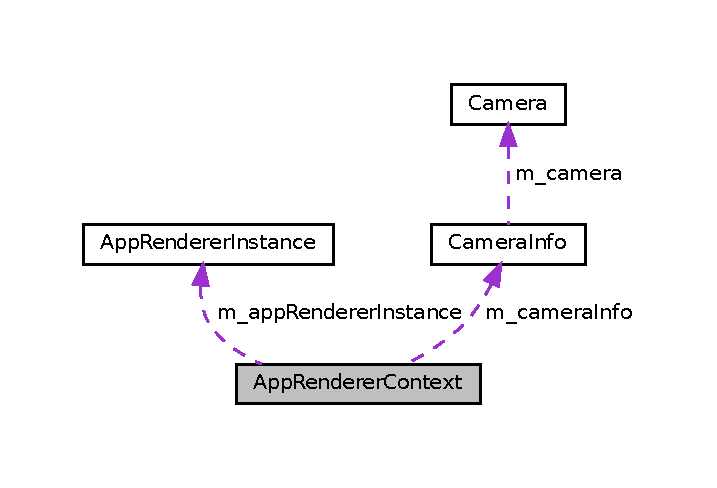
\includegraphics[width=344pt]{structAppRendererContext__coll__graph}
\end{center}
\end{figure}
\subsection*{Public Member Functions}
\begin{DoxyCompactItemize}
\item 
\mbox{\Hypertarget{structAppRendererContext_a19db4ff8090083fbc6150a818acc4ec2}\label{structAppRendererContext_a19db4ff8090083fbc6150a818acc4ec2}} 
{\bfseries App\+Renderer\+Context} (const \hyperlink{structCameraInfo}{Camera\+Info} \&camera\+Info)
\end{DoxyCompactItemize}
\subsection*{Public Attributes}
\begin{DoxyCompactItemize}
\item 
\mbox{\Hypertarget{structAppRendererContext_aefb7ea01003d765275701a26d9a037e9}\label{structAppRendererContext_aefb7ea01003d765275701a26d9a037e9}} 
\hyperlink{classAppRendererInstance}{App\+Renderer\+Instance} $\ast$ {\bfseries m\+\_\+app\+Renderer\+Instance}
\item 
\mbox{\Hypertarget{structAppRendererContext_aec7039b02cfe5358658ede445b68f33f}\label{structAppRendererContext_aec7039b02cfe5358658ede445b68f33f}} 
\hyperlink{structCameraInfo}{Camera\+Info} {\bfseries m\+\_\+camera\+Info}
\end{DoxyCompactItemize}


The documentation for this struct was generated from the following file\+:\begin{DoxyCompactItemize}
\item 
Graphics/App\+Renderer\+Instance.\+h\end{DoxyCompactItemize}

\hypertarget{classAppRendererInstance}{}\section{App\+Renderer\+Instance Class Reference}
\label{classAppRendererInstance}\index{App\+Renderer\+Instance@{App\+Renderer\+Instance}}
\subsection*{Public Member Functions}
\begin{DoxyCompactItemize}
\item 
\mbox{\Hypertarget{classAppRendererInstance_a515b2caf02195a031e72d2c6e2763e33}\label{classAppRendererInstance_a515b2caf02195a031e72d2c6e2763e33}} 
{\bfseries App\+Renderer\+Instance} (\hyperlink{classAppRenderer}{App\+Renderer} $\ast$app\+Renderer, \hyperlink{classDXRenderer}{D\+X\+Renderer} $\ast$dxrenderer, const \hyperlink{structCameraInfo}{Camera\+Info} \&camera\+Info)
\item 
\mbox{\Hypertarget{classAppRendererInstance_add1e6dadf22e4f6c37c5ff2d3a0139ea}\label{classAppRendererInstance_add1e6dadf22e4f6c37c5ff2d3a0139ea}} 
void {\bfseries Update} (float dt)
\item 
\mbox{\Hypertarget{classAppRendererInstance_af812f24fea366355d8c8f0932fdc05f8}\label{classAppRendererInstance_af812f24fea366355d8c8f0932fdc05f8}} 
void {\bfseries Render} ()
\item 
\mbox{\Hypertarget{classAppRendererInstance_a7ef8162fb5bed1b3b5151fc9478fe393}\label{classAppRendererInstance_a7ef8162fb5bed1b3b5151fc9478fe393}} 
void {\bfseries Initialize} ()
\item 
\mbox{\Hypertarget{classAppRendererInstance_ac33e5065fc392f5d948e5c5ed3b41e67}\label{classAppRendererInstance_ac33e5065fc392f5d948e5c5ed3b41e67}} 
void {\bfseries Load\+Content} ()
\item 
\mbox{\Hypertarget{classAppRendererInstance_aa08022e4f7a93586ad0017b024b30265}\label{classAppRendererInstance_aa08022e4f7a93586ad0017b024b30265}} 
void {\bfseries Release} ()
\end{DoxyCompactItemize}
\subsection*{Friends}
\begin{DoxyCompactItemize}
\item 
\mbox{\Hypertarget{classAppRendererInstance_a7bec99218ac38952a4baa8888bc7fedc}\label{classAppRendererInstance_a7bec99218ac38952a4baa8888bc7fedc}} 
class {\bfseries Deferred\+Rendering\+Instance}
\item 
\mbox{\Hypertarget{classAppRendererInstance_aa2fce3a4ae64b69f01e0fd64ba26023a}\label{classAppRendererInstance_aa2fce3a4ae64b69f01e0fd64ba26023a}} 
class {\bfseries Debug\+Rendering\+Instance}
\item 
\mbox{\Hypertarget{classAppRendererInstance_af2b4490c4b9be86b986502e67885f591}\label{classAppRendererInstance_af2b4490c4b9be86b986502e67885f591}} 
class {\bfseries M\+S\+A\+A\+Resolve\+Pass\+Instance}
\item 
\mbox{\Hypertarget{classAppRendererInstance_aba9f3240241811e775ef4280a9df4333}\label{classAppRendererInstance_aba9f3240241811e775ef4280a9df4333}} 
class {\bfseries Particle\+Rendering\+Instance}
\item 
\mbox{\Hypertarget{classAppRendererInstance_af8087aef5ebe8f9a42bfabe1e0672728}\label{classAppRendererInstance_af8087aef5ebe8f9a42bfabe1e0672728}} 
class {\bfseries U\+I\+Object\+Rendering\+Instance}
\item 
\mbox{\Hypertarget{classAppRendererInstance_a5532c3b535b4f2a814054dba701936df}\label{classAppRendererInstance_a5532c3b535b4f2a814054dba701936df}} 
class {\bfseries Text\+Rendering\+Instance}
\item 
\mbox{\Hypertarget{classAppRendererInstance_a5f3d064e51c4a3bf9409801632b9a7af}\label{classAppRendererInstance_a5f3d064e51c4a3bf9409801632b9a7af}} 
class {\bfseries App\+Renderer}
\end{DoxyCompactItemize}


The documentation for this class was generated from the following files\+:\begin{DoxyCompactItemize}
\item 
Graphics/App\+Renderer\+Instance.\+h\item 
Graphics/App\+Renderer\+Instance.\+cpp\end{DoxyCompactItemize}

\hypertarget{structArcLengthData}{}\section{Arc\+Length\+Data Struct Reference}
\label{structArcLengthData}\index{Arc\+Length\+Data@{Arc\+Length\+Data}}
\subsection*{Public Attributes}
\begin{DoxyCompactItemize}
\item 
\mbox{\Hypertarget{structArcLengthData_a9eb61e1228b5955c2f17b656b6034330}\label{structArcLengthData_a9eb61e1228b5955c2f17b656b6034330}} 
float {\bfseries s}
\item 
\mbox{\Hypertarget{structArcLengthData_aa40e451c1fb61467c393a3ad41515789}\label{structArcLengthData_aa40e451c1fb61467c393a3ad41515789}} 
float {\bfseries dist}
\end{DoxyCompactItemize}


The documentation for this struct was generated from the following file\+:\begin{DoxyCompactItemize}
\item 
Components/Follow\+Curves\+Path\+Component.\+h\end{DoxyCompactItemize}

\hypertarget{classAudioManager}{}\section{Audio\+Manager Class Reference}
\label{classAudioManager}\index{Audio\+Manager@{Audio\+Manager}}


Reacts to song and sfx events.  




{\ttfamily \#include $<$Audio\+Manager.\+h$>$}

\subsection*{Public Member Functions}
\begin{DoxyCompactItemize}
\item 
void \hyperlink{classAudioManager_a7c46b6078950fdb622672bf10c58e87e}{Play\+S\+FX} (\hyperlink{classStringId}{String\+Id} p\+File)
\begin{DoxyCompactList}\small\item\em Play S\+FX file path (must be preloaded) \end{DoxyCompactList}\item 
void \hyperlink{classAudioManager_a50184981af15f336b986cffb5e6c57d3}{Play\+Song} (\hyperlink{classStringId}{String\+Id} p\+File)
\begin{DoxyCompactList}\small\item\em Play song file path (must be preloaded) \end{DoxyCompactList}\item 
\hyperlink{classStringId}{String\+Id} \hyperlink{classAudioManager_ac1a61ce7acbbb62fa5b8f56870a8f674}{Get\+Current\+Song} () const
\begin{DoxyCompactList}\small\item\em Get the Current Playing song name. \end{DoxyCompactList}\item 
\mbox{\Hypertarget{classAudioManager_a6f046330684dee2f1e2c0bcffde5a9b2}\label{classAudioManager_a6f046330684dee2f1e2c0bcffde5a9b2}} 
void \hyperlink{classAudioManager_a6f046330684dee2f1e2c0bcffde5a9b2}{Stop\+S\+FX} ()
\begin{DoxyCompactList}\small\item\em Stop S\+FX Channel. \end{DoxyCompactList}\item 
\mbox{\Hypertarget{classAudioManager_a51bdb4c55fa5bf1f538c281fe8a16fad}\label{classAudioManager_a51bdb4c55fa5bf1f538c281fe8a16fad}} 
void \hyperlink{classAudioManager_a51bdb4c55fa5bf1f538c281fe8a16fad}{Stop\+Song} ()
\begin{DoxyCompactList}\small\item\em Stop Song Channel. \end{DoxyCompactList}\item 
\mbox{\Hypertarget{classAudioManager_a9df0bd203bd954ebb927656d4acbff16}\label{classAudioManager_a9df0bd203bd954ebb927656d4acbff16}} 
void \hyperlink{classAudioManager_a9df0bd203bd954ebb927656d4acbff16}{Pause\+Song} ()
\begin{DoxyCompactList}\small\item\em Pause Song. \end{DoxyCompactList}\item 
\mbox{\Hypertarget{classAudioManager_ad97f762b267c2fb4e6aeb7e6df2e857d}\label{classAudioManager_ad97f762b267c2fb4e6aeb7e6df2e857d}} 
void \hyperlink{classAudioManager_ad97f762b267c2fb4e6aeb7e6df2e857d}{Continue\+Song} ()
\begin{DoxyCompactList}\small\item\em Continue Playing Song. \end{DoxyCompactList}\item 
void \hyperlink{classAudioManager_a10dac004e0e76079f6b9b94cdd4a9469}{Set\+Master\+Volume} (float volume)
\begin{DoxyCompactList}\small\item\em Set the Master Volume. \end{DoxyCompactList}\item 
\mbox{\Hypertarget{classAudioManager_a99acf81981086c54966746ac1b6cf6a0}\label{classAudioManager_a99acf81981086c54966746ac1b6cf6a0}} 
void {\bfseries Increment\+Master\+Volume} ()
\item 
\mbox{\Hypertarget{classAudioManager_a399089557fd7fe5eaa3b1874f668c649}\label{classAudioManager_a399089557fd7fe5eaa3b1874f668c649}} 
void {\bfseries Decrement\+Slider\+Volume} ()
\item 
void \hyperlink{classAudioManager_a6f9e78a71e1046bf4f13baad2adff4c3}{Set\+S\+F\+X\+Volume} (float volume)
\begin{DoxyCompactList}\small\item\em Set the S\+FX Volume. \end{DoxyCompactList}\item 
\mbox{\Hypertarget{classAudioManager_aa66b52132b93cdd54978cb150505fa08}\label{classAudioManager_aa66b52132b93cdd54978cb150505fa08}} 
void {\bfseries Increment\+S\+F\+X\+Volume} ()
\item 
\mbox{\Hypertarget{classAudioManager_aa486a36bcc936a5529c97dea6e78a536}\label{classAudioManager_aa486a36bcc936a5529c97dea6e78a536}} 
void {\bfseries Decrement\+S\+F\+X\+Volume} ()
\item 
void \hyperlink{classAudioManager_acc31d4056bfdcfff325a91bcd583b8a0}{Set\+Song\+Volume} (float volume)
\begin{DoxyCompactList}\small\item\em Set the Song Volume. \end{DoxyCompactList}\item 
\mbox{\Hypertarget{classAudioManager_a8d47c27a446ed51eb8a3a3f51fc4d2fb}\label{classAudioManager_a8d47c27a446ed51eb8a3a3f51fc4d2fb}} 
void {\bfseries Increment\+Song\+Volume} ()
\item 
\mbox{\Hypertarget{classAudioManager_ab500238a1a478a9325fdcaf1538d26cb}\label{classAudioManager_ab500238a1a478a9325fdcaf1538d26cb}} 
void {\bfseries Decrement\+Song\+Volume} ()
\item 
void \hyperlink{classAudioManager_a0c203bcb774ef51b949a7e20f598630a}{Update} (float dt)
\begin{DoxyCompactList}\small\item\em Per frame update Used for fade-\/in fade-\/out related changes. \end{DoxyCompactList}\item 
void \hyperlink{classAudioManager_a37c83447f25569c6dc6b1d022230ad70}{Check\+Error} (F\+M\+O\+D\+\_\+\+R\+E\+S\+U\+LT result)
\begin{DoxyCompactList}\small\item\em Check the F\+M\+OD Error. \end{DoxyCompactList}\end{DoxyCompactItemize}
\subsection*{Friends}
\begin{DoxyCompactItemize}
\item 
\mbox{\Hypertarget{classAudioManager_a54c1252abc87a78a301e6b6984470408}\label{classAudioManager_a54c1252abc87a78a301e6b6984470408}} 
class {\bfseries Resource\+Manager}
\end{DoxyCompactItemize}


\subsection{Detailed Description}
Reacts to song and sfx events. 

\subsection{Member Function Documentation}
\mbox{\Hypertarget{classAudioManager_a37c83447f25569c6dc6b1d022230ad70}\label{classAudioManager_a37c83447f25569c6dc6b1d022230ad70}} 
\index{Audio\+Manager@{Audio\+Manager}!Check\+Error@{Check\+Error}}
\index{Check\+Error@{Check\+Error}!Audio\+Manager@{Audio\+Manager}}
\subsubsection{\texorpdfstring{Check\+Error()}{CheckError()}}
{\footnotesize\ttfamily void Audio\+Manager\+::\+Check\+Error (\begin{DoxyParamCaption}\item[{F\+M\+O\+D\+\_\+\+R\+E\+S\+U\+LT}]{result }\end{DoxyParamCaption})}



Check the F\+M\+OD Error. 


\begin{DoxyParams}{Parameters}
{\em result} & \\
\hline
\end{DoxyParams}
\mbox{\Hypertarget{classAudioManager_ac1a61ce7acbbb62fa5b8f56870a8f674}\label{classAudioManager_ac1a61ce7acbbb62fa5b8f56870a8f674}} 
\index{Audio\+Manager@{Audio\+Manager}!Get\+Current\+Song@{Get\+Current\+Song}}
\index{Get\+Current\+Song@{Get\+Current\+Song}!Audio\+Manager@{Audio\+Manager}}
\subsubsection{\texorpdfstring{Get\+Current\+Song()}{GetCurrentSong()}}
{\footnotesize\ttfamily \hyperlink{classStringId}{String\+Id} Audio\+Manager\+::\+Get\+Current\+Song (\begin{DoxyParamCaption}{ }\end{DoxyParamCaption}) const}



Get the Current Playing song name. 

\begin{DoxyReturn}{Returns}
\hyperlink{classStringId}{String\+Id} 
\end{DoxyReturn}
\mbox{\Hypertarget{classAudioManager_a7c46b6078950fdb622672bf10c58e87e}\label{classAudioManager_a7c46b6078950fdb622672bf10c58e87e}} 
\index{Audio\+Manager@{Audio\+Manager}!Play\+S\+FX@{Play\+S\+FX}}
\index{Play\+S\+FX@{Play\+S\+FX}!Audio\+Manager@{Audio\+Manager}}
\subsubsection{\texorpdfstring{Play\+S\+F\+X()}{PlaySFX()}}
{\footnotesize\ttfamily void Audio\+Manager\+::\+Play\+S\+FX (\begin{DoxyParamCaption}\item[{\hyperlink{classStringId}{String\+Id}}]{p\+File }\end{DoxyParamCaption})}



Play S\+FX file path (must be preloaded) 


\begin{DoxyParams}{Parameters}
{\em p\+File} & \\
\hline
\end{DoxyParams}
\mbox{\Hypertarget{classAudioManager_a50184981af15f336b986cffb5e6c57d3}\label{classAudioManager_a50184981af15f336b986cffb5e6c57d3}} 
\index{Audio\+Manager@{Audio\+Manager}!Play\+Song@{Play\+Song}}
\index{Play\+Song@{Play\+Song}!Audio\+Manager@{Audio\+Manager}}
\subsubsection{\texorpdfstring{Play\+Song()}{PlaySong()}}
{\footnotesize\ttfamily void Audio\+Manager\+::\+Play\+Song (\begin{DoxyParamCaption}\item[{\hyperlink{classStringId}{String\+Id}}]{p\+File }\end{DoxyParamCaption})}



Play song file path (must be preloaded) 


\begin{DoxyParams}{Parameters}
{\em p\+File} & \\
\hline
\end{DoxyParams}
\mbox{\Hypertarget{classAudioManager_a10dac004e0e76079f6b9b94cdd4a9469}\label{classAudioManager_a10dac004e0e76079f6b9b94cdd4a9469}} 
\index{Audio\+Manager@{Audio\+Manager}!Set\+Master\+Volume@{Set\+Master\+Volume}}
\index{Set\+Master\+Volume@{Set\+Master\+Volume}!Audio\+Manager@{Audio\+Manager}}
\subsubsection{\texorpdfstring{Set\+Master\+Volume()}{SetMasterVolume()}}
{\footnotesize\ttfamily void Audio\+Manager\+::\+Set\+Master\+Volume (\begin{DoxyParamCaption}\item[{float}]{volume }\end{DoxyParamCaption})}



Set the Master Volume. 


\begin{DoxyParams}{Parameters}
{\em volume} & 0-\/100 \\
\hline
\end{DoxyParams}
\mbox{\Hypertarget{classAudioManager_a6f9e78a71e1046bf4f13baad2adff4c3}\label{classAudioManager_a6f9e78a71e1046bf4f13baad2adff4c3}} 
\index{Audio\+Manager@{Audio\+Manager}!Set\+S\+F\+X\+Volume@{Set\+S\+F\+X\+Volume}}
\index{Set\+S\+F\+X\+Volume@{Set\+S\+F\+X\+Volume}!Audio\+Manager@{Audio\+Manager}}
\subsubsection{\texorpdfstring{Set\+S\+F\+X\+Volume()}{SetSFXVolume()}}
{\footnotesize\ttfamily void Audio\+Manager\+::\+Set\+S\+F\+X\+Volume (\begin{DoxyParamCaption}\item[{float}]{volume }\end{DoxyParamCaption})}



Set the S\+FX Volume. 


\begin{DoxyParams}{Parameters}
{\em volume} & 0-\/100 \\
\hline
\end{DoxyParams}
\mbox{\Hypertarget{classAudioManager_acc31d4056bfdcfff325a91bcd583b8a0}\label{classAudioManager_acc31d4056bfdcfff325a91bcd583b8a0}} 
\index{Audio\+Manager@{Audio\+Manager}!Set\+Song\+Volume@{Set\+Song\+Volume}}
\index{Set\+Song\+Volume@{Set\+Song\+Volume}!Audio\+Manager@{Audio\+Manager}}
\subsubsection{\texorpdfstring{Set\+Song\+Volume()}{SetSongVolume()}}
{\footnotesize\ttfamily void Audio\+Manager\+::\+Set\+Song\+Volume (\begin{DoxyParamCaption}\item[{float}]{volume }\end{DoxyParamCaption})}



Set the Song Volume. 


\begin{DoxyParams}{Parameters}
{\em volume} & 0-\/100 \\
\hline
\end{DoxyParams}
\mbox{\Hypertarget{classAudioManager_a0c203bcb774ef51b949a7e20f598630a}\label{classAudioManager_a0c203bcb774ef51b949a7e20f598630a}} 
\index{Audio\+Manager@{Audio\+Manager}!Update@{Update}}
\index{Update@{Update}!Audio\+Manager@{Audio\+Manager}}
\subsubsection{\texorpdfstring{Update()}{Update()}}
{\footnotesize\ttfamily void Audio\+Manager\+::\+Update (\begin{DoxyParamCaption}\item[{float}]{dt }\end{DoxyParamCaption})}



Per frame update Used for fade-\/in fade-\/out related changes. 


\begin{DoxyParams}{Parameters}
{\em dt} & \\
\hline
\end{DoxyParams}


The documentation for this class was generated from the following files\+:\begin{DoxyCompactItemize}
\item 
Managers/\hyperlink{AudioManager_8h}{Audio\+Manager.\+h}\item 
Managers/Audio\+Manager.\+cpp\end{DoxyCompactItemize}

\hypertarget{structBakedSkyboxIrradianceInstanceData}{}\section{Baked\+Skybox\+Irradiance\+Instance\+Data Struct Reference}
\label{structBakedSkyboxIrradianceInstanceData}\index{Baked\+Skybox\+Irradiance\+Instance\+Data@{Baked\+Skybox\+Irradiance\+Instance\+Data}}


Collaboration diagram for Baked\+Skybox\+Irradiance\+Instance\+Data\+:\nopagebreak
\begin{figure}[H]
\begin{center}
\leavevmode
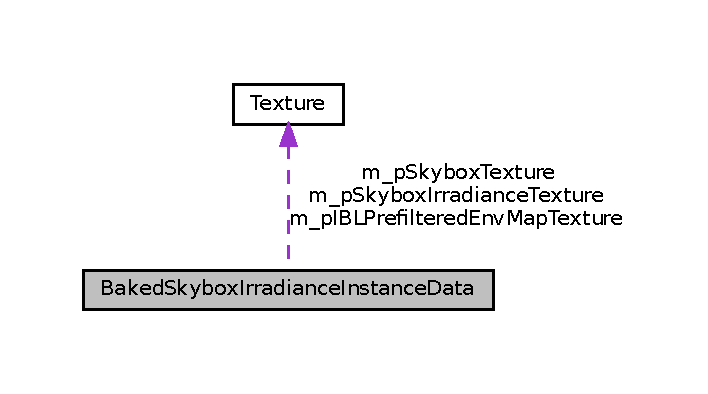
\includegraphics[width=340pt]{structBakedSkyboxIrradianceInstanceData__coll__graph}
\end{center}
\end{figure}
\subsection*{Public Attributes}
\begin{DoxyCompactItemize}
\item 
\mbox{\Hypertarget{structBakedSkyboxIrradianceInstanceData_a10ffb1ec82b0032da7b632e87725117a}\label{structBakedSkyboxIrradianceInstanceData_a10ffb1ec82b0032da7b632e87725117a}} 
\hyperlink{classTexture}{Texture} $\ast$ {\bfseries m\+\_\+p\+Skybox\+Texture}
\item 
\mbox{\Hypertarget{structBakedSkyboxIrradianceInstanceData_abff80b70eb17d661cf39c5260eb21711}\label{structBakedSkyboxIrradianceInstanceData_abff80b70eb17d661cf39c5260eb21711}} 
\hyperlink{classTexture}{Texture} $\ast$ {\bfseries m\+\_\+p\+Skybox\+Irradiance\+Texture}
\item 
\mbox{\Hypertarget{structBakedSkyboxIrradianceInstanceData_ad5a3b447d6cf3e8fb7363216b5c19043}\label{structBakedSkyboxIrradianceInstanceData_ad5a3b447d6cf3e8fb7363216b5c19043}} 
\hyperlink{classTexture}{Texture} $\ast$ {\bfseries m\+\_\+p\+I\+B\+L\+Prefiltered\+Env\+Map\+Texture}
\end{DoxyCompactItemize}


The documentation for this struct was generated from the following file\+:\begin{DoxyCompactItemize}
\item 
Graphics/Instance\+Render\+Data.\+h\end{DoxyCompactItemize}

\hypertarget{classBaseCallback}{}\section{Base\+Callback Class Reference}
\label{classBaseCallback}\index{Base\+Callback@{Base\+Callback}}


Base \hyperlink{classEvent}{Event} Callback Class that is mirrored for Base\+Events. Carries function callback pointer.  




{\ttfamily \#include $<$Event\+Callback.\+h$>$}



Inheritance diagram for Base\+Callback\+:
\nopagebreak
\begin{figure}[H]
\begin{center}
\leavevmode
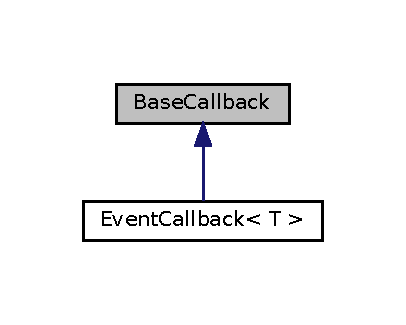
\includegraphics[width=195pt]{classBaseCallback__inherit__graph}
\end{center}
\end{figure}
\subsection*{Public Types}
\begin{DoxyCompactItemize}
\item 
\mbox{\Hypertarget{classBaseCallback_a20c1623e166841cea02948e54122690a}\label{classBaseCallback_a20c1623e166841cea02948e54122690a}} 
typedef std\+::unique\+\_\+ptr$<$ \hyperlink{classBaseCallback}{Base\+Callback} $>$ {\bfseries Ptr}
\end{DoxyCompactItemize}
\subsection*{Public Member Functions}
\begin{DoxyCompactItemize}
\item 
\hyperlink{classBaseCallback_a9071b9dda8d9a997937670f7ec4edcea}{Base\+Callback} (const void $\ast$\+\_\+owner)
\begin{DoxyCompactList}\small\item\em Construct a new Base Callback object. \end{DoxyCompactList}\item 
const void $\ast$ \hyperlink{classBaseCallback_ad9ea4e795a92a1c91b38596dbca29da3}{Get\+Owner} () const
\begin{DoxyCompactList}\small\item\em Get the owner\textquotesingle{}s pointer (used for book-\/keeping) \end{DoxyCompactList}\item 
virtual void \hyperlink{classBaseCallback_af87d16a88aaf3c429e5f020798f97a8b}{Call} (const void $\ast$event)=0
\begin{DoxyCompactList}\small\item\em Call bound function passing inherited event in non abstract function. \end{DoxyCompactList}\end{DoxyCompactItemize}
\subsection*{Protected Attributes}
\begin{DoxyCompactItemize}
\item 
\mbox{\Hypertarget{classBaseCallback_a9f44b039af4ffe1c7bcdeaddd10e2bbd}\label{classBaseCallback_a9f44b039af4ffe1c7bcdeaddd10e2bbd}} 
const void $\ast$ {\bfseries m\+\_\+owner}
\end{DoxyCompactItemize}


\subsection{Detailed Description}
Base \hyperlink{classEvent}{Event} Callback Class that is mirrored for Base\+Events. Carries function callback pointer. 

\subsection{Constructor \& Destructor Documentation}
\mbox{\Hypertarget{classBaseCallback_a9071b9dda8d9a997937670f7ec4edcea}\label{classBaseCallback_a9071b9dda8d9a997937670f7ec4edcea}} 
\index{Base\+Callback@{Base\+Callback}!Base\+Callback@{Base\+Callback}}
\index{Base\+Callback@{Base\+Callback}!Base\+Callback@{Base\+Callback}}
\subsubsection{\texorpdfstring{Base\+Callback()}{BaseCallback()}}
{\footnotesize\ttfamily Base\+Callback\+::\+Base\+Callback (\begin{DoxyParamCaption}\item[{const void $\ast$}]{\+\_\+owner }\end{DoxyParamCaption})\hspace{0.3cm}{\ttfamily [inline]}}



Construct a new Base Callback object. 


\begin{DoxyParams}{Parameters}
{\em \+\_\+owner} & Pointer to owning object\textquotesingle{}s pointer in memory (used for book-\/keeping) \\
\hline
\end{DoxyParams}


\subsection{Member Function Documentation}
\mbox{\Hypertarget{classBaseCallback_af87d16a88aaf3c429e5f020798f97a8b}\label{classBaseCallback_af87d16a88aaf3c429e5f020798f97a8b}} 
\index{Base\+Callback@{Base\+Callback}!Call@{Call}}
\index{Call@{Call}!Base\+Callback@{Base\+Callback}}
\subsubsection{\texorpdfstring{Call()}{Call()}}
{\footnotesize\ttfamily virtual void Base\+Callback\+::\+Call (\begin{DoxyParamCaption}\item[{const void $\ast$}]{event }\end{DoxyParamCaption})\hspace{0.3cm}{\ttfamily [pure virtual]}}



Call bound function passing inherited event in non abstract function. 


\begin{DoxyParams}{Parameters}
{\em event} & \\
\hline
\end{DoxyParams}


Implemented in \hyperlink{classEventCallback_ad34e4a69e56733e07342d0c56cd15dfc}{Event\+Callback$<$ T $>$}.

\mbox{\Hypertarget{classBaseCallback_ad9ea4e795a92a1c91b38596dbca29da3}\label{classBaseCallback_ad9ea4e795a92a1c91b38596dbca29da3}} 
\index{Base\+Callback@{Base\+Callback}!Get\+Owner@{Get\+Owner}}
\index{Get\+Owner@{Get\+Owner}!Base\+Callback@{Base\+Callback}}
\subsubsection{\texorpdfstring{Get\+Owner()}{GetOwner()}}
{\footnotesize\ttfamily const void$\ast$ Base\+Callback\+::\+Get\+Owner (\begin{DoxyParamCaption}{ }\end{DoxyParamCaption}) const\hspace{0.3cm}{\ttfamily [inline]}}



Get the owner\textquotesingle{}s pointer (used for book-\/keeping) 

\begin{DoxyReturn}{Returns}
const void$\ast$ 
\end{DoxyReturn}


The documentation for this class was generated from the following file\+:\begin{DoxyCompactItemize}
\item 
Events/\hyperlink{EventCallback_8h}{Event\+Callback.\+h}\end{DoxyCompactItemize}

\hypertarget{classBaseComponent}{}\section{Base\+Component Class Reference}
\label{classBaseComponent}\index{Base\+Component@{Base\+Component}}


Base class for all components (engine and scripted)  




{\ttfamily \#include $<$Base\+Component.\+h$>$}



Inheritance diagram for Base\+Component\+:
\nopagebreak
\begin{figure}[H]
\begin{center}
\leavevmode
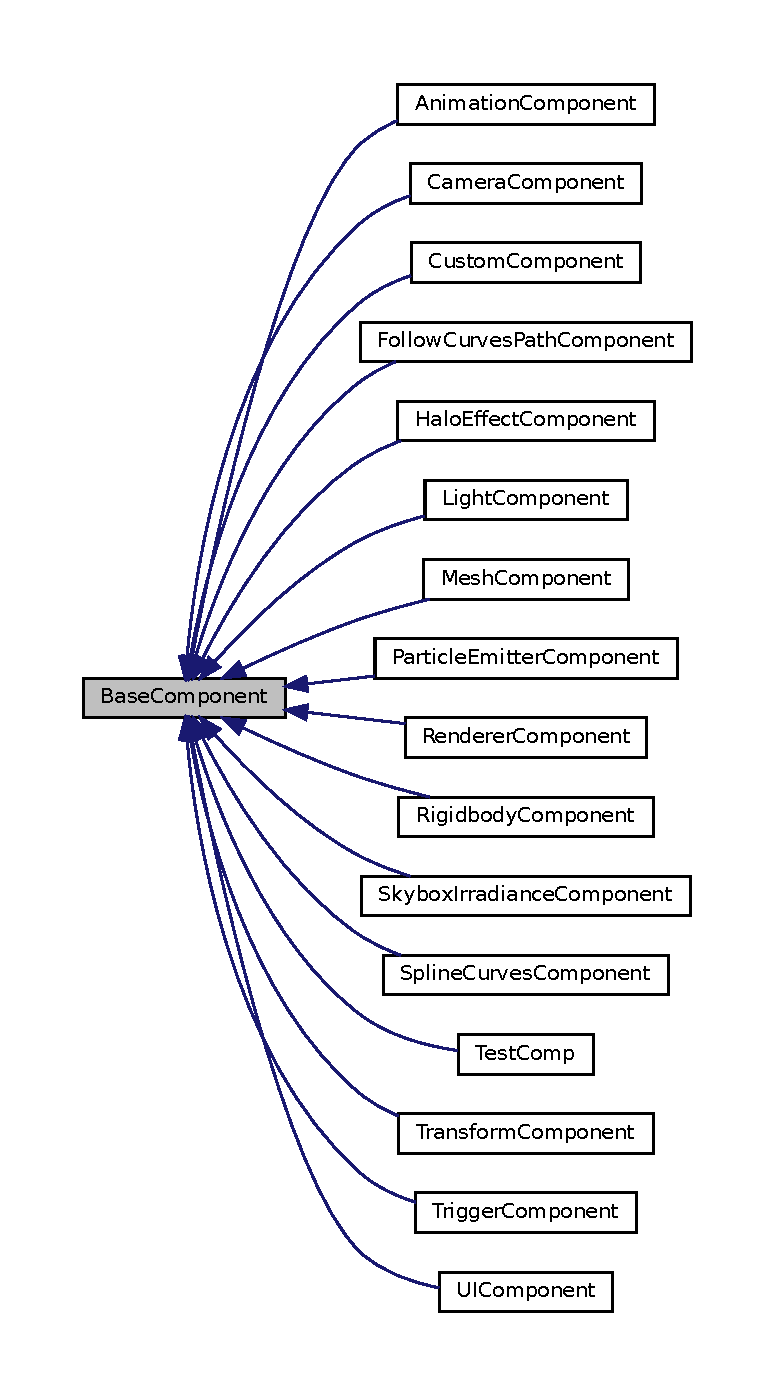
\includegraphics[height=550pt]{classBaseComponent__inherit__graph}
\end{center}
\end{figure}


Collaboration diagram for Base\+Component\+:
\nopagebreak
\begin{figure}[H]
\begin{center}
\leavevmode
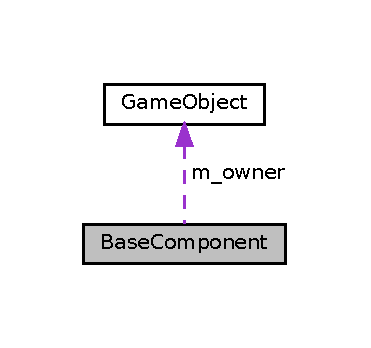
\includegraphics[width=178pt]{classBaseComponent__coll__graph}
\end{center}
\end{figure}
\subsection*{Public Types}
\begin{DoxyCompactItemize}
\item 
\mbox{\Hypertarget{classBaseComponent_a1815699cb565ac2ec254cf61174015cf}\label{classBaseComponent_a1815699cb565ac2ec254cf61174015cf}} 
typedef unsigned int {\bfseries Component\+Id}
\end{DoxyCompactItemize}
\subsection*{Public Member Functions}
\begin{DoxyCompactItemize}
\item 
\hyperlink{classBaseComponent_a64d22c1f5eb72a53ed7584e24f55fcfe}{Base\+Component} (\hyperlink{classGameObject}{Game\+Object} $\ast$owner, Component\+Id type)
\begin{DoxyCompactList}\small\item\em Construct a new Base Component object. \end{DoxyCompactList}\item 
\mbox{\Hypertarget{classBaseComponent_ab281730e838c4cb33e96ab6d6b7fe15f}\label{classBaseComponent_ab281730e838c4cb33e96ab6d6b7fe15f}} 
virtual \hyperlink{classBaseComponent_ab281730e838c4cb33e96ab6d6b7fe15f}{$\sim$\+Base\+Component} ()
\begin{DoxyCompactList}\small\item\em Destroy the Base Component object. \end{DoxyCompactList}\item 
Component\+Id \hyperlink{classBaseComponent_a50e4481cdb27430cf4a5a10f1a06af35}{Get\+Type} () const
\begin{DoxyCompactList}\small\item\em Get the Type object. \end{DoxyCompactList}\item 
\hyperlink{classGameObject}{Game\+Object} $\ast$ \hyperlink{classBaseComponent_aa07f9b9c2ebdd2c314404771857e9e07}{Get\+Owner} () const
\begin{DoxyCompactList}\small\item\em Get the Owner object. \end{DoxyCompactList}\end{DoxyCompactItemize}
\subsection*{Protected Member Functions}
\begin{DoxyCompactItemize}
\item 
\mbox{\Hypertarget{classBaseComponent_a3fe4f92f22cd488107f2929b7545d878}\label{classBaseComponent_a3fe4f92f22cd488107f2929b7545d878}} 
{\bfseries R\+T\+T\+R\+\_\+\+E\+N\+A\+B\+LE} ()
\end{DoxyCompactItemize}
\subsection*{Protected Attributes}
\begin{DoxyCompactItemize}
\item 
\mbox{\Hypertarget{classBaseComponent_ae4de98b70923b6c515ced3a97b2f3d32}\label{classBaseComponent_ae4de98b70923b6c515ced3a97b2f3d32}} 
Component\+Id \hyperlink{classBaseComponent_ae4de98b70923b6c515ced3a97b2f3d32}{m\+\_\+type}
\begin{DoxyCompactList}\small\item\em Id unique per component type. \end{DoxyCompactList}\item 
\mbox{\Hypertarget{classBaseComponent_a0b7f35e80a5033c8ba721f40927e6e75}\label{classBaseComponent_a0b7f35e80a5033c8ba721f40927e6e75}} 
\hyperlink{classGameObject}{Game\+Object} $\ast$ \hyperlink{classBaseComponent_a0b7f35e80a5033c8ba721f40927e6e75}{m\+\_\+owner}
\begin{DoxyCompactList}\small\item\em Pointer to \hyperlink{classGameObject}{Game\+Object} owner of this component. \end{DoxyCompactList}\item 
\mbox{\Hypertarget{classBaseComponent_a0d398cc5055095b7b8aa5a0f6f054ad1}\label{classBaseComponent_a0d398cc5055095b7b8aa5a0f6f054ad1}} 
{\bfseries R\+T\+T\+R\+\_\+\+R\+E\+G\+I\+S\+T\+R\+A\+T\+I\+O\+N\+\_\+\+F\+R\+I\+E\+ND}
\end{DoxyCompactItemize}
\subsection*{Static Protected Attributes}
\begin{DoxyCompactItemize}
\item 
\mbox{\Hypertarget{classBaseComponent_a084ade347bc71a7f0d3b17ecdc2225a4}\label{classBaseComponent_a084ade347bc71a7f0d3b17ecdc2225a4}} 
static Component\+Id \hyperlink{classBaseComponent_a084ade347bc71a7f0d3b17ecdc2225a4}{number\+Of\+Types} = 0
\begin{DoxyCompactList}\small\item\em Static member, number of unique component types. \end{DoxyCompactList}\end{DoxyCompactItemize}
\subsection*{Friends}
\begin{DoxyCompactItemize}
\item 
\mbox{\Hypertarget{classBaseComponent_a328c093d609680cca505905c6d49901a}\label{classBaseComponent_a328c093d609680cca505905c6d49901a}} 
class {\bfseries Factory}
\item 
\mbox{\Hypertarget{classBaseComponent_a00df87c957d8f7ee0fc51f07a0542f4a}\label{classBaseComponent_a00df87c957d8f7ee0fc51f07a0542f4a}} 
class {\bfseries Game\+Object}
\end{DoxyCompactItemize}


\subsection{Detailed Description}
Base class for all components (engine and scripted) 

\subsection{Constructor \& Destructor Documentation}
\mbox{\Hypertarget{classBaseComponent_a64d22c1f5eb72a53ed7584e24f55fcfe}\label{classBaseComponent_a64d22c1f5eb72a53ed7584e24f55fcfe}} 
\index{Base\+Component@{Base\+Component}!Base\+Component@{Base\+Component}}
\index{Base\+Component@{Base\+Component}!Base\+Component@{Base\+Component}}
\subsubsection{\texorpdfstring{Base\+Component()}{BaseComponent()}}
{\footnotesize\ttfamily Base\+Component\+::\+Base\+Component (\begin{DoxyParamCaption}\item[{\hyperlink{classGameObject}{Game\+Object} $\ast$}]{owner,  }\item[{Component\+Id}]{type }\end{DoxyParamCaption})\hspace{0.3cm}{\ttfamily [inline]}}



Construct a new Base Component object. 


\begin{DoxyParams}{Parameters}
{\em owner} & \\
\hline
{\em type} & \\
\hline
\end{DoxyParams}


\subsection{Member Function Documentation}
\mbox{\Hypertarget{classBaseComponent_aa07f9b9c2ebdd2c314404771857e9e07}\label{classBaseComponent_aa07f9b9c2ebdd2c314404771857e9e07}} 
\index{Base\+Component@{Base\+Component}!Get\+Owner@{Get\+Owner}}
\index{Get\+Owner@{Get\+Owner}!Base\+Component@{Base\+Component}}
\subsubsection{\texorpdfstring{Get\+Owner()}{GetOwner()}}
{\footnotesize\ttfamily \hyperlink{classGameObject}{Game\+Object}$\ast$ Base\+Component\+::\+Get\+Owner (\begin{DoxyParamCaption}{ }\end{DoxyParamCaption}) const\hspace{0.3cm}{\ttfamily [inline]}}



Get the Owner object. 

\begin{DoxyReturn}{Returns}
Game\+Object$\ast$ 
\end{DoxyReturn}
\mbox{\Hypertarget{classBaseComponent_a50e4481cdb27430cf4a5a10f1a06af35}\label{classBaseComponent_a50e4481cdb27430cf4a5a10f1a06af35}} 
\index{Base\+Component@{Base\+Component}!Get\+Type@{Get\+Type}}
\index{Get\+Type@{Get\+Type}!Base\+Component@{Base\+Component}}
\subsubsection{\texorpdfstring{Get\+Type()}{GetType()}}
{\footnotesize\ttfamily Component\+Id Base\+Component\+::\+Get\+Type (\begin{DoxyParamCaption}{ }\end{DoxyParamCaption}) const\hspace{0.3cm}{\ttfamily [inline]}}



Get the Type object. 

\begin{DoxyReturn}{Returns}
Component\+Id 
\end{DoxyReturn}


The documentation for this class was generated from the following files\+:\begin{DoxyCompactItemize}
\item 
Components/\hyperlink{BaseComponent_8h}{Base\+Component.\+h}\item 
Components/Base\+Component.\+cpp\end{DoxyCompactItemize}

\hypertarget{classBaseEvent}{}\section{Base\+Event Class Reference}
\label{classBaseEvent}\index{Base\+Event@{Base\+Event}}


Base \hyperlink{classEvent}{Event} Class that is mirrored for event callbacks.  




{\ttfamily \#include $<$Base\+Event.\+h$>$}



Inheritance diagram for Base\+Event\+:
\nopagebreak
\begin{figure}[H]
\begin{center}
\leavevmode
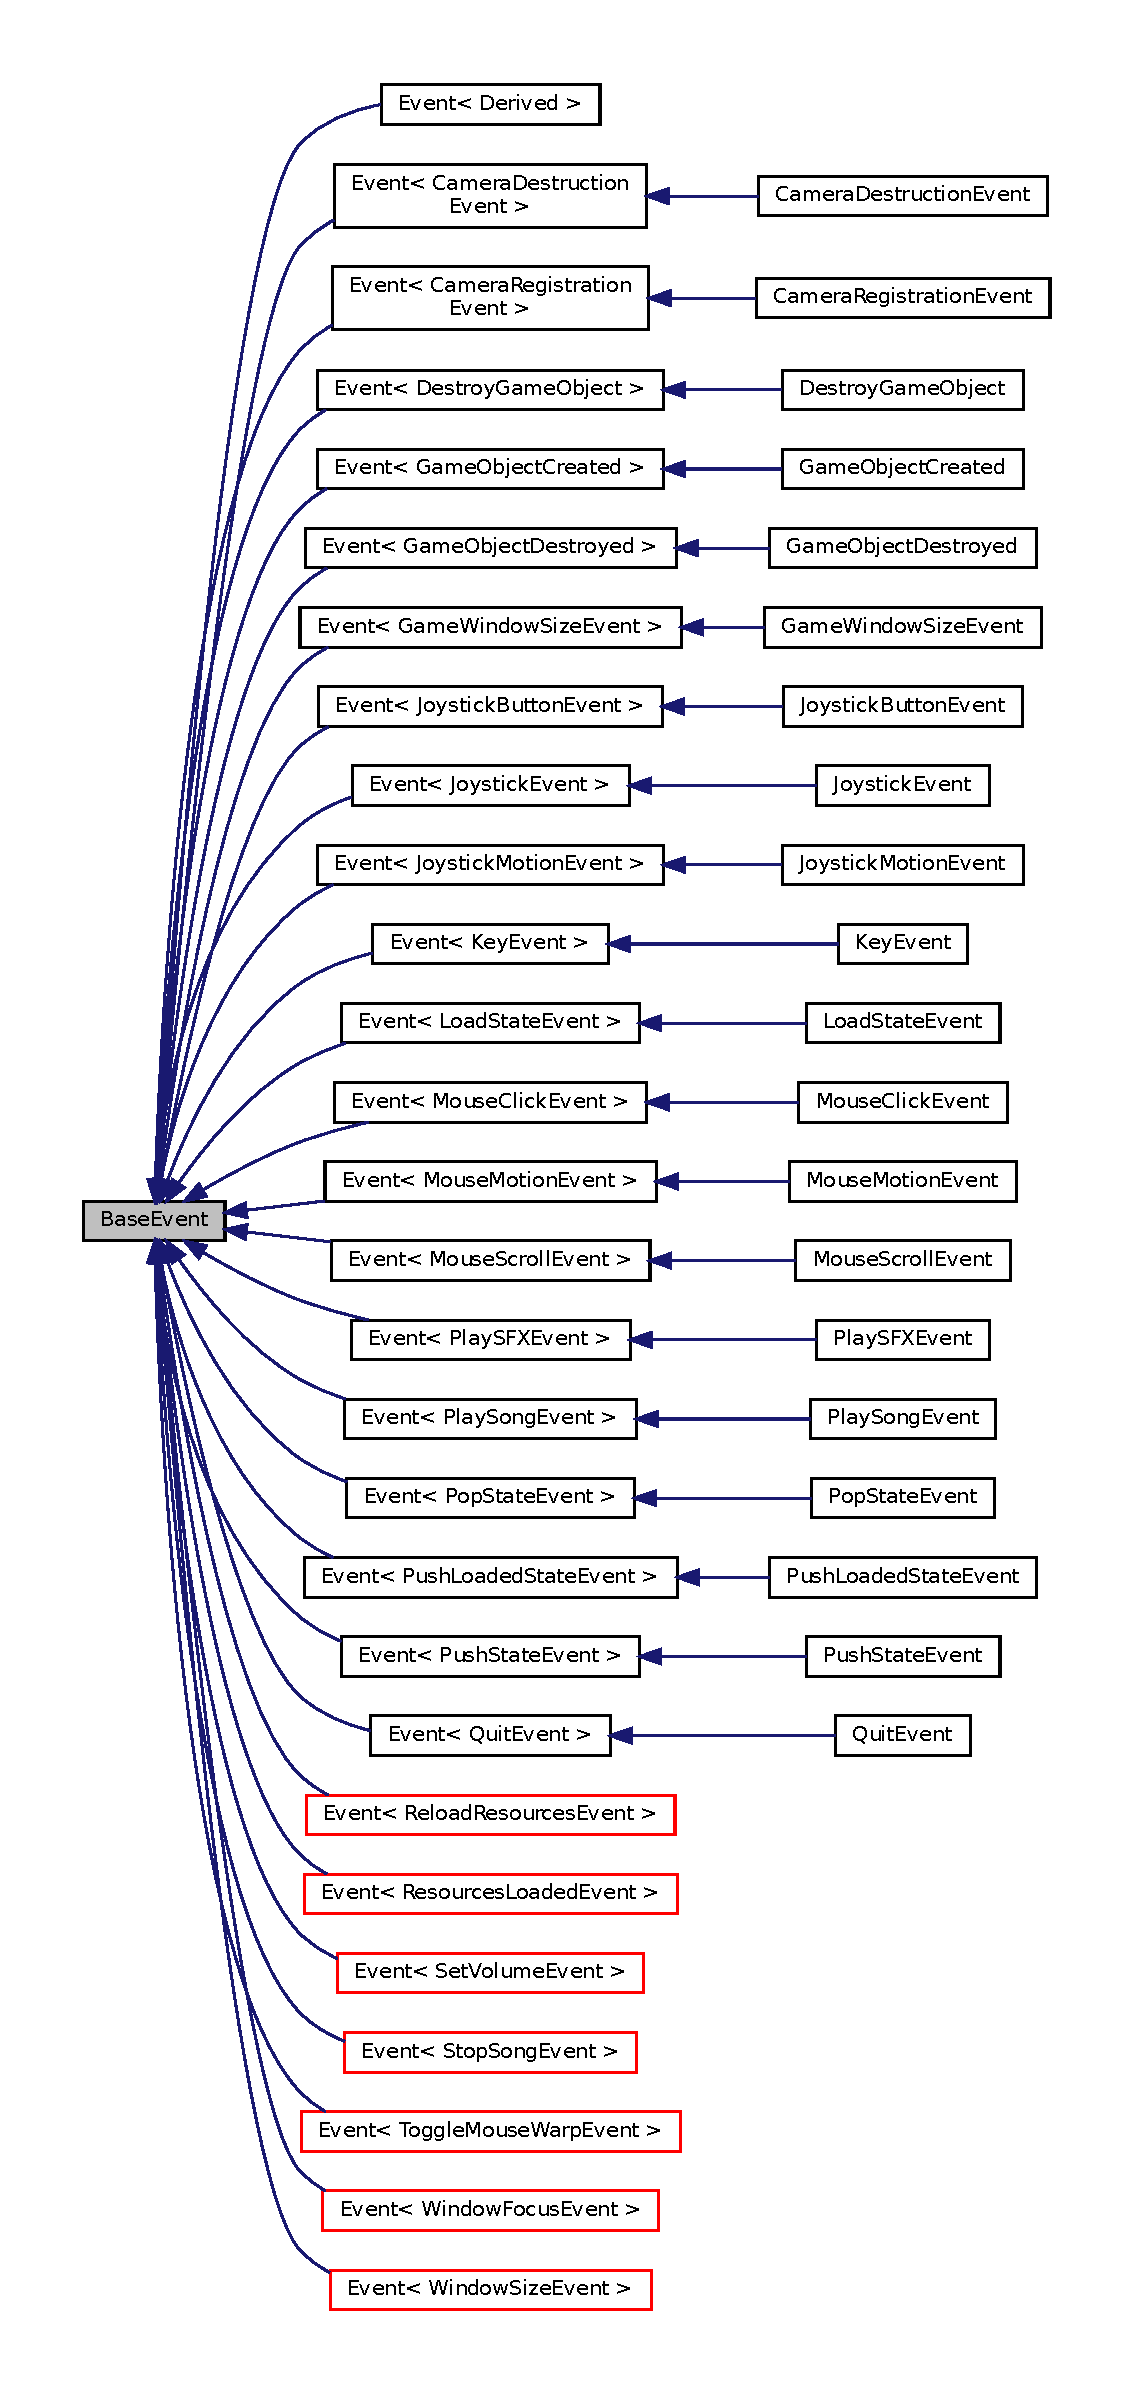
\includegraphics[height=550pt]{classBaseEvent__inherit__graph}
\end{center}
\end{figure}
\subsection*{Public Types}
\begin{DoxyCompactItemize}
\item 
\mbox{\Hypertarget{classBaseEvent_a67cfea4f5876d7644ffe71c460b77e62}\label{classBaseEvent_a67cfea4f5876d7644ffe71c460b77e62}} 
typedef std\+::size\+\_\+t {\bfseries Event\+Id}
\item 
\mbox{\Hypertarget{classBaseEvent_adcd2734dcd54d458c8a6a2cbdac14d19}\label{classBaseEvent_adcd2734dcd54d458c8a6a2cbdac14d19}} 
typedef std\+::unique\+\_\+ptr$<$ \hyperlink{classBaseEvent}{Base\+Event} $>$ {\bfseries Ptr}
\end{DoxyCompactItemize}
\subsection*{Public Member Functions}
\begin{DoxyCompactItemize}
\item 
\mbox{\Hypertarget{classBaseEvent_afa6860ba23bb43a7e158d238939c265f}\label{classBaseEvent_afa6860ba23bb43a7e158d238939c265f}} 
virtual void \hyperlink{classBaseEvent_afa6860ba23bb43a7e158d238939c265f}{operator()} ()=0
\begin{DoxyCompactList}\small\item\em Virtual function for mirror multicast invoke when event is invoked This is useful with some events for script delegate binds. \end{DoxyCompactList}\end{DoxyCompactItemize}
\subsection*{Public Attributes}
\begin{DoxyCompactItemize}
\item 
\mbox{\Hypertarget{classBaseEvent_afb79121ea0c7c6de301353e5e2fe3a34}\label{classBaseEvent_afb79121ea0c7c6de301353e5e2fe3a34}} 
float \hyperlink{classBaseEvent_afb79121ea0c7c6de301353e5e2fe3a34}{m\+\_\+delay}
\begin{DoxyCompactList}\small\item\em Time Delay before executing event. \end{DoxyCompactList}\end{DoxyCompactItemize}
\subsection*{Static Protected Attributes}
\begin{DoxyCompactItemize}
\item 
\mbox{\Hypertarget{classBaseEvent_a4e5bcc9ddaf500a7093357a00be5aa02}\label{classBaseEvent_a4e5bcc9ddaf500a7093357a00be5aa02}} 
static Event\+Id {\bfseries m\+\_\+event\+Id}
\end{DoxyCompactItemize}
\subsection*{Friends}
\begin{DoxyCompactItemize}
\item 
\mbox{\Hypertarget{classBaseEvent_aba45a46c615e2683daffdae82e2d3b8f}\label{classBaseEvent_aba45a46c615e2683daffdae82e2d3b8f}} 
class {\bfseries Event\+Manager}
\end{DoxyCompactItemize}


\subsection{Detailed Description}
Base \hyperlink{classEvent}{Event} Class that is mirrored for event callbacks. 

The documentation for this class was generated from the following files\+:\begin{DoxyCompactItemize}
\item 
Events/\hyperlink{BaseEvent_8h}{Base\+Event.\+h}\item 
Events/Base\+Event.\+cpp\end{DoxyCompactItemize}

\hypertarget{classBaseSystem}{}\section{Base\+System Class Reference}
\label{classBaseSystem}\index{Base\+System@{Base\+System}}


Base class for Systems.  




{\ttfamily \#include $<$Base\+System.\+h$>$}



Inheritance diagram for Base\+System\+:
\nopagebreak
\begin{figure}[H]
\begin{center}
\leavevmode
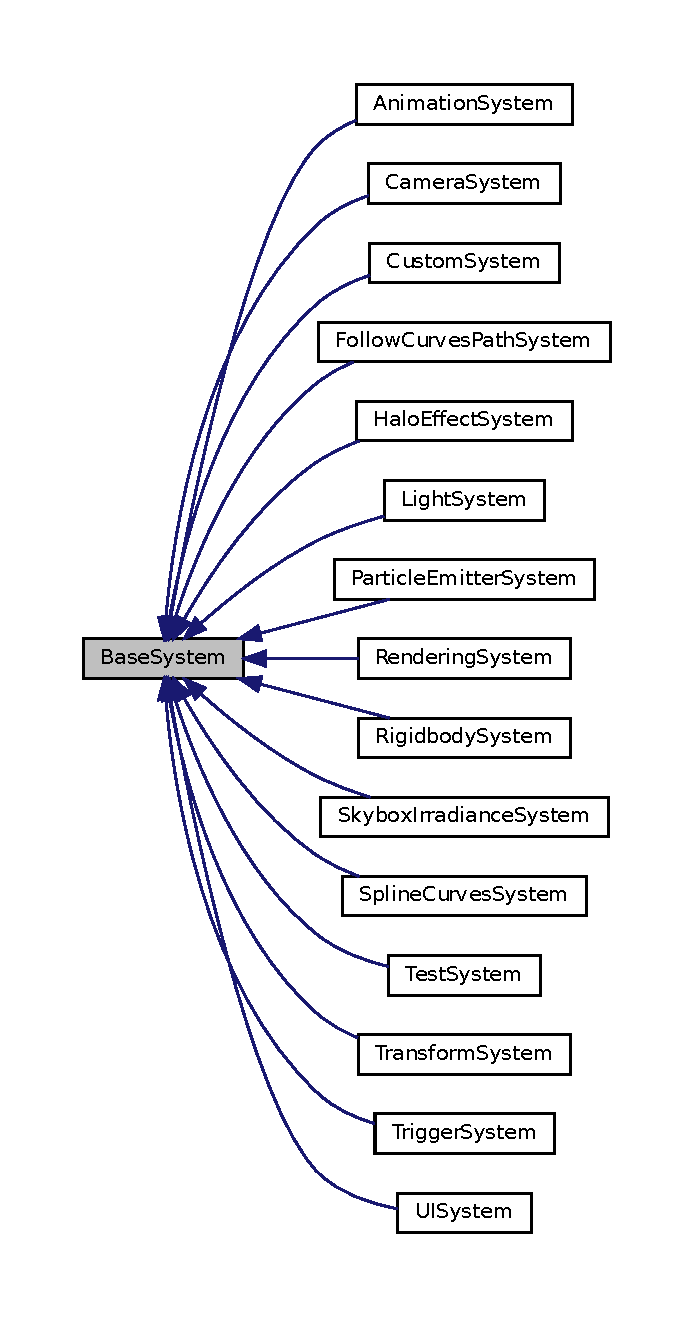
\includegraphics[height=550pt]{classBaseSystem__inherit__graph}
\end{center}
\end{figure}
\subsection*{Public Member Functions}
\begin{DoxyCompactItemize}
\item 
\mbox{\Hypertarget{classBaseSystem_a77a342bf74a7e875f35ff1c70dd8c310}\label{classBaseSystem_a77a342bf74a7e875f35ff1c70dd8c310}} 
\hyperlink{classBaseSystem_a77a342bf74a7e875f35ff1c70dd8c310}{Base\+System} ()
\begin{DoxyCompactList}\small\item\em Constructor for base class. Called by inheriting classes. \end{DoxyCompactList}\item 
\mbox{\Hypertarget{classBaseSystem_a581856f116f41009f84ae359aef588b3}\label{classBaseSystem_a581856f116f41009f84ae359aef588b3}} 
virtual \hyperlink{classBaseSystem_a581856f116f41009f84ae359aef588b3}{$\sim$\+Base\+System} ()
\begin{DoxyCompactList}\small\item\em Destroy the Base System object. \end{DoxyCompactList}\item 
virtual void \hyperlink{classBaseSystem_a202ed394e663f970f181d810c86760dc}{Early\+Update} (float dt)
\begin{DoxyCompactList}\small\item\em Early update called once before main Update. When called, you have access to every \hyperlink{classGameObject}{Game\+Object} registered and can manage interaction between them. \end{DoxyCompactList}\item 
void \hyperlink{classBaseSystem_a6422693fc429d74a2b0b4c4e860d1810}{Update\+All\+Nodes} (float dt)
\begin{DoxyCompactList}\small\item\em Iterates through all Game\+Objects registered and calls update. \end{DoxyCompactList}\item 
virtual void \hyperlink{classBaseSystem_ab6520975a6376e59005d3a40456358d4}{Late\+Update} (float dt)
\begin{DoxyCompactList}\small\item\em Late update called once after main Update. When called, you have access to every \hyperlink{classGameObject}{Game\+Object} registered and can manage interaction between them. \end{DoxyCompactList}\item 
virtual void \hyperlink{classBaseSystem_a465191589a1ef8b8f3a8e20fa4656d47}{Update} (float dt, \hyperlink{structBaseSystemCompNode}{Base\+System\+Comp\+Node} $\ast$comp\+Node)
\begin{DoxyCompactList}\small\item\em Regular Update call. Called once per registered \hyperlink{classGameObject}{Game\+Object} by Update\+All\+Nodes. \end{DoxyCompactList}\item 
\mbox{\Hypertarget{classBaseSystem_a94339337789820c707da572d140a0923}\label{classBaseSystem_a94339337789820c707da572d140a0923}} 
virtual void \hyperlink{classBaseSystem_a94339337789820c707da572d140a0923}{Draw} (float dt, \hyperlink{structBaseSystemCompNode}{Base\+System\+Comp\+Node} $\ast$comp\+Node)
\begin{DoxyCompactList}\small\item\em Regular Draw call. Called once per registered \hyperlink{classGameObject}{Game\+Object} by Draw\+All\+Nodes. \end{DoxyCompactList}\item 
void \hyperlink{classBaseSystem_af8f5ce5a033d06bd9aeb944d2a193e74}{Draw\+All\+Nodes} (float dt)
\begin{DoxyCompactList}\small\item\em Iterates through all registered Game\+Objects and calls Draw. \end{DoxyCompactList}\end{DoxyCompactItemize}
\subsection*{Protected Member Functions}
\begin{DoxyCompactItemize}
\item 
{\footnotesize template$<$typename T $>$ }\\void \hyperlink{classBaseSystem_a672d8b7902414c5a4b46d10f5f403785}{Push\+\_\+required\+\_\+comp} ()
\begin{DoxyCompactList}\small\item\em Used to setup the system, so for every registered \hyperlink{classGameObject}{Game\+Object} node, we have pointer to the components that are updated on this system. \end{DoxyCompactList}\end{DoxyCompactItemize}
\subsection*{Protected Attributes}
\begin{DoxyCompactItemize}
\item 
\mbox{\Hypertarget{classBaseSystem_ab0f0418b57f4f6fdfb12fa6f317c1921}\label{classBaseSystem_ab0f0418b57f4f6fdfb12fa6f317c1921}} 
std\+::bitset$<$ M\+A\+X\+\_\+\+N\+U\+M\+\_\+\+C\+O\+M\+P\+O\+N\+E\+N\+TS $>$ \hyperlink{classBaseSystem_ab0f0418b57f4f6fdfb12fa6f317c1921}{m\+\_\+required\+Comp\+Mask}
\begin{DoxyCompactList}\small\item\em Byteset used to mask against Game\+Objects component mask and check if they can register. \end{DoxyCompactList}\item 
\mbox{\Hypertarget{classBaseSystem_a24b890d25ee0eeed44ef6976c7188224}\label{classBaseSystem_a24b890d25ee0eeed44ef6976c7188224}} 
std\+::unordered\+\_\+map$<$ size\+\_\+t, \hyperlink{structBaseSystemCompNode}{Base\+System\+Comp\+Node} $\ast$ $>$ \hyperlink{classBaseSystem_a24b890d25ee0eeed44ef6976c7188224}{m\+\_\+\+Obj\+Components\+Map}
\begin{DoxyCompactList}\small\item\em Hash map holding the nodes of registered Game\+Objects components. \end{DoxyCompactList}\end{DoxyCompactItemize}
\subsection*{Static Protected Attributes}
\begin{DoxyCompactItemize}
\item 
\mbox{\Hypertarget{classBaseSystem_a7ef356edab3cfb02905e0a73a645b131}\label{classBaseSystem_a7ef356edab3cfb02905e0a73a645b131}} 
static unsigned int \hyperlink{classBaseSystem_a7ef356edab3cfb02905e0a73a645b131}{number\+Of\+Types} = 0
\begin{DoxyCompactList}\small\item\em Static member. Number of system types. \end{DoxyCompactList}\end{DoxyCompactItemize}
\subsection*{Friends}
\begin{DoxyCompactItemize}
\item 
\mbox{\Hypertarget{classBaseSystem_a328c093d609680cca505905c6d49901a}\label{classBaseSystem_a328c093d609680cca505905c6d49901a}} 
class {\bfseries Factory}
\item 
\mbox{\Hypertarget{classBaseSystem_ab1ef2aa9992dd8ae85793e1a1f980e1e}\label{classBaseSystem_ab1ef2aa9992dd8ae85793e1a1f980e1e}} 
class {\bfseries System\+Manager}
\end{DoxyCompactItemize}


\subsection{Detailed Description}
Base class for Systems. 

\subsection{Member Function Documentation}
\mbox{\Hypertarget{classBaseSystem_af8f5ce5a033d06bd9aeb944d2a193e74}\label{classBaseSystem_af8f5ce5a033d06bd9aeb944d2a193e74}} 
\index{Base\+System@{Base\+System}!Draw\+All\+Nodes@{Draw\+All\+Nodes}}
\index{Draw\+All\+Nodes@{Draw\+All\+Nodes}!Base\+System@{Base\+System}}
\subsubsection{\texorpdfstring{Draw\+All\+Nodes()}{DrawAllNodes()}}
{\footnotesize\ttfamily void Base\+System\+::\+Draw\+All\+Nodes (\begin{DoxyParamCaption}\item[{float}]{dt }\end{DoxyParamCaption})}



Iterates through all registered Game\+Objects and calls Draw. 


\begin{DoxyParams}{Parameters}
{\em dt} & \\
\hline
\end{DoxyParams}
\mbox{\Hypertarget{classBaseSystem_a202ed394e663f970f181d810c86760dc}\label{classBaseSystem_a202ed394e663f970f181d810c86760dc}} 
\index{Base\+System@{Base\+System}!Early\+Update@{Early\+Update}}
\index{Early\+Update@{Early\+Update}!Base\+System@{Base\+System}}
\subsubsection{\texorpdfstring{Early\+Update()}{EarlyUpdate()}}
{\footnotesize\ttfamily virtual void Base\+System\+::\+Early\+Update (\begin{DoxyParamCaption}\item[{float}]{dt }\end{DoxyParamCaption})\hspace{0.3cm}{\ttfamily [inline]}, {\ttfamily [virtual]}}



Early update called once before main Update. When called, you have access to every \hyperlink{classGameObject}{Game\+Object} registered and can manage interaction between them. 


\begin{DoxyParams}{Parameters}
{\em dt} & \\
\hline
\end{DoxyParams}


Reimplemented in \hyperlink{classUISystem_ac7e49ca17db397a2321a8b89dbc5bd47}{U\+I\+System}.

\mbox{\Hypertarget{classBaseSystem_ab6520975a6376e59005d3a40456358d4}\label{classBaseSystem_ab6520975a6376e59005d3a40456358d4}} 
\index{Base\+System@{Base\+System}!Late\+Update@{Late\+Update}}
\index{Late\+Update@{Late\+Update}!Base\+System@{Base\+System}}
\subsubsection{\texorpdfstring{Late\+Update()}{LateUpdate()}}
{\footnotesize\ttfamily virtual void Base\+System\+::\+Late\+Update (\begin{DoxyParamCaption}\item[{float}]{dt }\end{DoxyParamCaption})\hspace{0.3cm}{\ttfamily [inline]}, {\ttfamily [virtual]}}



Late update called once after main Update. When called, you have access to every \hyperlink{classGameObject}{Game\+Object} registered and can manage interaction between them. 


\begin{DoxyParams}{Parameters}
{\em dt} & \\
\hline
\end{DoxyParams}


Reimplemented in \hyperlink{classRigidbodySystem_a3ae11c7e5a8572247fb2e01729e32af9}{Rigidbody\+System}, and \hyperlink{classTriggerSystem_a804c490350677fea99a385b1f22a85b6}{Trigger\+System}.

\mbox{\Hypertarget{classBaseSystem_a672d8b7902414c5a4b46d10f5f403785}\label{classBaseSystem_a672d8b7902414c5a4b46d10f5f403785}} 
\index{Base\+System@{Base\+System}!Push\+\_\+required\+\_\+comp@{Push\+\_\+required\+\_\+comp}}
\index{Push\+\_\+required\+\_\+comp@{Push\+\_\+required\+\_\+comp}!Base\+System@{Base\+System}}
\subsubsection{\texorpdfstring{Push\+\_\+required\+\_\+comp()}{Push\_required\_comp()}}
{\footnotesize\ttfamily template$<$typename T $>$ \\
void Base\+System\+::\+Push\+\_\+required\+\_\+comp (\begin{DoxyParamCaption}{ }\end{DoxyParamCaption})\hspace{0.3cm}{\ttfamily [protected]}}



Used to setup the system, so for every registered \hyperlink{classGameObject}{Game\+Object} node, we have pointer to the components that are updated on this system. 


\begin{DoxyTemplParams}{Template Parameters}
{\em T} & \\
\hline
\end{DoxyTemplParams}
\mbox{\Hypertarget{classBaseSystem_a465191589a1ef8b8f3a8e20fa4656d47}\label{classBaseSystem_a465191589a1ef8b8f3a8e20fa4656d47}} 
\index{Base\+System@{Base\+System}!Update@{Update}}
\index{Update@{Update}!Base\+System@{Base\+System}}
\subsubsection{\texorpdfstring{Update()}{Update()}}
{\footnotesize\ttfamily virtual void Base\+System\+::\+Update (\begin{DoxyParamCaption}\item[{float}]{dt,  }\item[{\hyperlink{structBaseSystemCompNode}{Base\+System\+Comp\+Node} $\ast$}]{comp\+Node }\end{DoxyParamCaption})\hspace{0.3cm}{\ttfamily [inline]}, {\ttfamily [virtual]}}



Regular Update call. Called once per registered \hyperlink{classGameObject}{Game\+Object} by Update\+All\+Nodes. 


\begin{DoxyParams}{Parameters}
{\em dt} & \\
\hline
{\em comp\+Node} & \\
\hline
\end{DoxyParams}


Reimplemented in \hyperlink{classCustomSystem_ab8b072ffd6b4de7404b385068d735c61}{Custom\+System}, \hyperlink{classAnimationSystem_aa74600f86761b9bb47a0689665901a49}{Animation\+System}, \hyperlink{classRenderingSystem_a658cdef75c3fc6d555347fb787eec460}{Rendering\+System}, \hyperlink{classTestSystem_a3742fdf321596824bc2aac8a91a3ddb0}{Test\+System}, \hyperlink{classTransformSystem_a75de8bdeda1137447d575b30d16afb3b}{Transform\+System}, \hyperlink{classSkyboxIrradianceSystem_ad1acf756b9540bb2864e5bf9631f9539}{Skybox\+Irradiance\+System}, \hyperlink{classParticleEmitterSystem_a58c14c4c3318b2fe31e35c93789da998}{Particle\+Emitter\+System}, \hyperlink{classHaloEffectSystem_ad98bff0ea12ef7d8abb1c917318e6028}{Halo\+Effect\+System}, \hyperlink{classSplineCurvesSystem_acc8b36c8c85662437bc2020f29e4d4b6}{Spline\+Curves\+System}, \hyperlink{classFollowCurvesPathSystem_a23f3ab7e281025eb8e40ef150a05a3b4}{Follow\+Curves\+Path\+System}, \hyperlink{classLightSystem_a492572de092cdbaf76c3ca4d9806df94}{Light\+System}, and \hyperlink{classCameraSystem_ab0ea25c2a8f704f0a0674a3bc61ddd68}{Camera\+System}.

\mbox{\Hypertarget{classBaseSystem_a6422693fc429d74a2b0b4c4e860d1810}\label{classBaseSystem_a6422693fc429d74a2b0b4c4e860d1810}} 
\index{Base\+System@{Base\+System}!Update\+All\+Nodes@{Update\+All\+Nodes}}
\index{Update\+All\+Nodes@{Update\+All\+Nodes}!Base\+System@{Base\+System}}
\subsubsection{\texorpdfstring{Update\+All\+Nodes()}{UpdateAllNodes()}}
{\footnotesize\ttfamily void Base\+System\+::\+Update\+All\+Nodes (\begin{DoxyParamCaption}\item[{float}]{dt }\end{DoxyParamCaption})}



Iterates through all Game\+Objects registered and calls update. 


\begin{DoxyParams}{Parameters}
{\em dt} & \\
\hline
\end{DoxyParams}


The documentation for this class was generated from the following files\+:\begin{DoxyCompactItemize}
\item 
Systems/\hyperlink{BaseSystem_8h}{Base\+System.\+h}\item 
Systems/Base\+System.\+cpp\end{DoxyCompactItemize}

\hypertarget{structBaseSystemCompNode}{}\section{Base\+System\+Comp\+Node Struct Reference}
\label{structBaseSystemCompNode}\index{Base\+System\+Comp\+Node@{Base\+System\+Comp\+Node}}


{\ttfamily \#include $<$Base\+System.\+h$>$}



Inheritance diagram for Base\+System\+Comp\+Node\+:\nopagebreak
\begin{figure}[H]
\begin{center}
\leavevmode
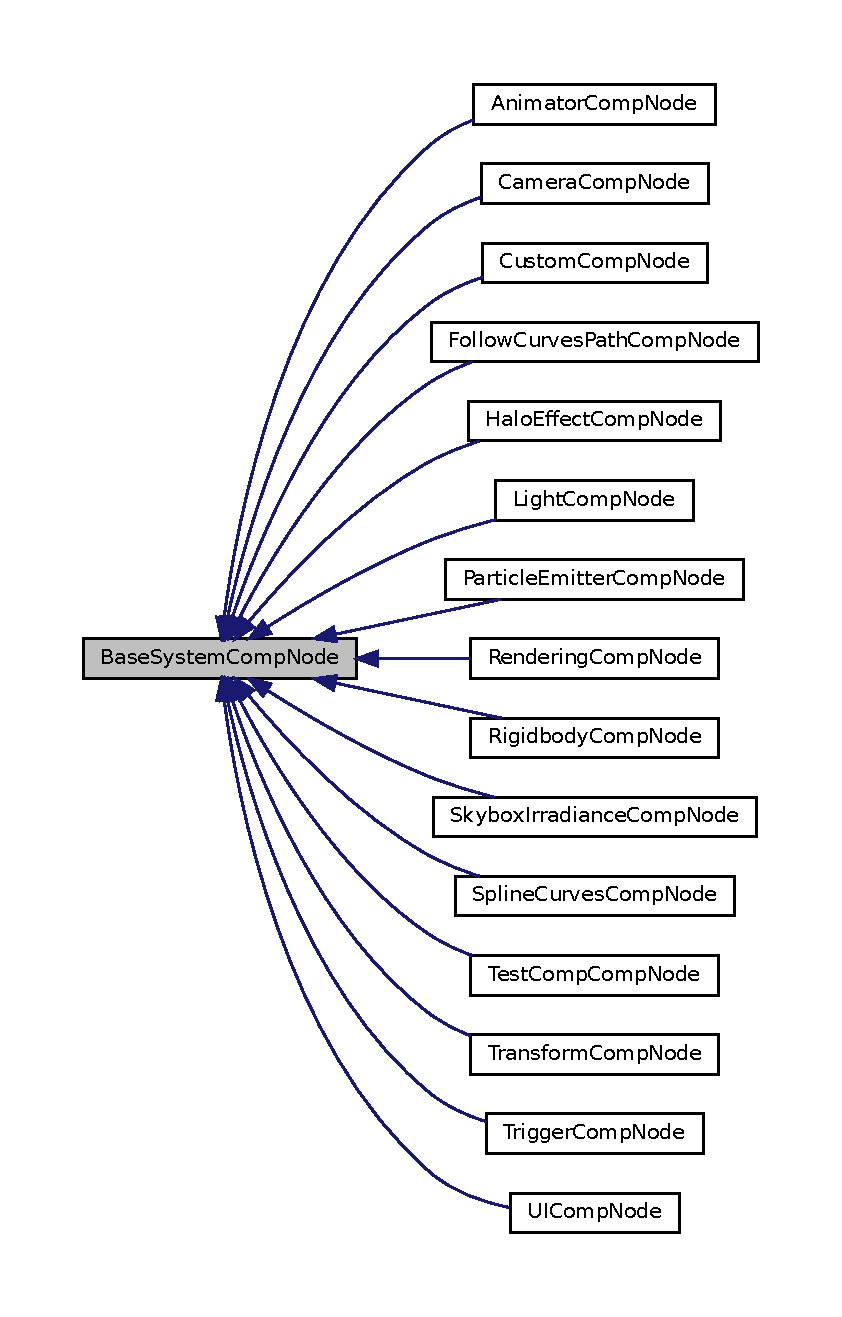
\includegraphics[width=350pt]{structBaseSystemCompNode__inherit__graph}
\end{center}
\end{figure}
\subsection*{Public Attributes}
\begin{DoxyCompactItemize}
\item 
\mbox{\Hypertarget{structBaseSystemCompNode_a5aa946abaae775c0bf3d9388712ee4ef}\label{structBaseSystemCompNode_a5aa946abaae775c0bf3d9388712ee4ef}} 
size\+\_\+t {\bfseries m\+\_\+go\+ID}
\end{DoxyCompactItemize}


\subsection{Detailed Description}
Includes include $<$bitset$>$ include $<$unordered\+\_\+map$>$ 

The documentation for this struct was generated from the following file\+:\begin{DoxyCompactItemize}
\item 
Systems/Base\+System.\+h\end{DoxyCompactItemize}

\hypertarget{classBlendState}{}\section{Blend\+State Class Reference}
\label{classBlendState}\index{Blend\+State@{Blend\+State}}
\subsection*{Public Member Functions}
\begin{DoxyCompactItemize}
\item 
\mbox{\Hypertarget{classBlendState_a7ea0025743426a3da3a0accd63c976c8}\label{classBlendState_a7ea0025743426a3da3a0accd63c976c8}} 
{\bfseries Blend\+State} (const \hyperlink{structBlendStateDesc}{Blend\+State\+Desc} \&blend\+\_\+state\+\_\+desc)
\item 
\mbox{\Hypertarget{classBlendState_a7c1b6e58093b0c33da63eae2742a7bed}\label{classBlendState_a7c1b6e58093b0c33da63eae2742a7bed}} 
void {\bfseries Release} ()
\end{DoxyCompactItemize}
\subsection*{Friends}
\begin{DoxyCompactItemize}
\item 
\mbox{\Hypertarget{classBlendState_a871268c492209c5a9db9dc2db99f4d04}\label{classBlendState_a871268c492209c5a9db9dc2db99f4d04}} 
class {\bfseries D\+X\+Resource\+Loader}
\item 
\mbox{\Hypertarget{classBlendState_a14ab6f966322dccbf6597d0c82bf48c6}\label{classBlendState_a14ab6f966322dccbf6597d0c82bf48c6}} 
class {\bfseries D\+X\+Renderer}
\end{DoxyCompactItemize}


The documentation for this class was generated from the following files\+:\begin{DoxyCompactItemize}
\item 
Graphics/Blend\+State.\+h\item 
Graphics/Blend\+State.\+cpp\end{DoxyCompactItemize}

\hypertarget{structBlendStateDesc}{}\section{Blend\+State\+Desc Struct Reference}
\label{structBlendStateDesc}\index{Blend\+State\+Desc@{Blend\+State\+Desc}}
\subsection*{Public Attributes}
\begin{DoxyCompactItemize}
\item 
\mbox{\Hypertarget{structBlendStateDesc_a0c86cbd4fce078055db85f2843aaec8f}\label{structBlendStateDesc_a0c86cbd4fce078055db85f2843aaec8f}} 
Blend\+Factor {\bfseries m\+\_\+src\+Factors} \mbox{[}M\+A\+X\+\_\+\+R\+E\+N\+D\+E\+R\+\_\+\+T\+A\+R\+G\+E\+T\+\_\+\+A\+T\+T\+A\+C\+H\+M\+E\+N\+TS\mbox{]}
\item 
\mbox{\Hypertarget{structBlendStateDesc_a748ebaebfe2a4b35bc8180d956c7bcd5}\label{structBlendStateDesc_a748ebaebfe2a4b35bc8180d956c7bcd5}} 
Blend\+Factor {\bfseries m\+\_\+dst\+Factors} \mbox{[}M\+A\+X\+\_\+\+R\+E\+N\+D\+E\+R\+\_\+\+T\+A\+R\+G\+E\+T\+\_\+\+A\+T\+T\+A\+C\+H\+M\+E\+N\+TS\mbox{]}
\item 
\mbox{\Hypertarget{structBlendStateDesc_acea0722e740bd902e964ec188a2c729e}\label{structBlendStateDesc_acea0722e740bd902e964ec188a2c729e}} 
Blend\+Factor {\bfseries m\+\_\+src\+Alpha\+Factors} \mbox{[}M\+A\+X\+\_\+\+R\+E\+N\+D\+E\+R\+\_\+\+T\+A\+R\+G\+E\+T\+\_\+\+A\+T\+T\+A\+C\+H\+M\+E\+N\+TS\mbox{]}
\item 
\mbox{\Hypertarget{structBlendStateDesc_a84ade16b8acda9aa3b1675f32218ed99}\label{structBlendStateDesc_a84ade16b8acda9aa3b1675f32218ed99}} 
Blend\+Factor {\bfseries m\+\_\+dst\+Alpha\+Factors} \mbox{[}M\+A\+X\+\_\+\+R\+E\+N\+D\+E\+R\+\_\+\+T\+A\+R\+G\+E\+T\+\_\+\+A\+T\+T\+A\+C\+H\+M\+E\+N\+TS\mbox{]}
\item 
\mbox{\Hypertarget{structBlendStateDesc_af3337b50096ac5ac2fd201a7bdfb4db6}\label{structBlendStateDesc_af3337b50096ac5ac2fd201a7bdfb4db6}} 
Blend\+Operator {\bfseries m\+\_\+blend\+Operator} \mbox{[}M\+A\+X\+\_\+\+R\+E\+N\+D\+E\+R\+\_\+\+T\+A\+R\+G\+E\+T\+\_\+\+A\+T\+T\+A\+C\+H\+M\+E\+N\+TS\mbox{]}
\item 
\mbox{\Hypertarget{structBlendStateDesc_a3f2fdfe6c8b2ade220adabc27735f007}\label{structBlendStateDesc_a3f2fdfe6c8b2ade220adabc27735f007}} 
Blend\+Operator {\bfseries m\+\_\+blend\+Alpha\+Operator} \mbox{[}M\+A\+X\+\_\+\+R\+E\+N\+D\+E\+R\+\_\+\+T\+A\+R\+G\+E\+T\+\_\+\+A\+T\+T\+A\+C\+H\+M\+E\+N\+TS\mbox{]}
\item 
\mbox{\Hypertarget{structBlendStateDesc_a2cb271eff4e45f9677697aca6df59e57}\label{structBlendStateDesc_a2cb271eff4e45f9677697aca6df59e57}} 
Blend\+State\+Targets {\bfseries m\+\_\+blend\+State\+Target}
\item 
\mbox{\Hypertarget{structBlendStateDesc_adf580099064524d75beea20700e81448}\label{structBlendStateDesc_adf580099064524d75beea20700e81448}} 
bool {\bfseries m\+\_\+enable\+Alpha\+Coverage}
\item 
\mbox{\Hypertarget{structBlendStateDesc_a28307d90a6efd7c4348ae493ae37332d}\label{structBlendStateDesc_a28307d90a6efd7c4348ae493ae37332d}} 
bool {\bfseries m\+\_\+individual\+Blend}
\end{DoxyCompactItemize}


The documentation for this struct was generated from the following file\+:\begin{DoxyCompactItemize}
\item 
Graphics/Blend\+State.\+h\end{DoxyCompactItemize}

\hypertarget{classBlurImagePass}{}\section{Blur\+Image\+Pass Class Reference}
\label{classBlurImagePass}\index{Blur\+Image\+Pass@{Blur\+Image\+Pass}}
\subsection*{Public Member Functions}
\begin{DoxyCompactItemize}
\item 
\mbox{\Hypertarget{classBlurImagePass_ab99b31ba1ad13f815e3664a8c11cd626}\label{classBlurImagePass_ab99b31ba1ad13f815e3664a8c11cd626}} 
{\bfseries Blur\+Image\+Pass} (\hyperlink{classAppRenderer}{App\+Renderer} $\ast$app\+\_\+renderer, Blur\+Channel blur\+\_\+channel=B\+L\+U\+R\+\_\+\+C\+H\+A\+N\+N\+E\+L\+\_\+\+O\+NE, uint32\+\_\+t blur\+\_\+width=8)
\item 
\mbox{\Hypertarget{classBlurImagePass_a668e5f8f964f342cb00b371d89fe316a}\label{classBlurImagePass_a668e5f8f964f342cb00b371d89fe316a}} 
void {\bfseries Release} ()
\item 
\mbox{\Hypertarget{classBlurImagePass_a7d7936da71ce4cfa0d5ef34f4cdc2c8f}\label{classBlurImagePass_a7d7936da71ce4cfa0d5ef34f4cdc2c8f}} 
void {\bfseries Blur\+Image} (\hyperlink{classTexture}{Texture} $\ast$input\+\_\+texture, \hyperlink{classTexture}{Texture} $\ast$intermediate\+\_\+texture, \hyperlink{classTexture}{Texture} $\ast$output\+\_\+texture\+\_\+to\+\_\+blur)
\item 
\mbox{\Hypertarget{classBlurImagePass_a254314dc7811669ece0db791ce20f089}\label{classBlurImagePass_a254314dc7811669ece0db791ce20f089}} 
void {\bfseries Load\+Content} (\hyperlink{classDXRenderer}{D\+X\+Renderer} $\ast$dxrenderer)
\item 
\mbox{\Hypertarget{classBlurImagePass_aa921dc3afee017718ade91551868addc}\label{classBlurImagePass_aa921dc3afee017718ade91551868addc}} 
void {\bfseries Set\+Blur\+Width} (uint32\+\_\+t blur\+\_\+width)
\end{DoxyCompactItemize}


The documentation for this class was generated from the following files\+:\begin{DoxyCompactItemize}
\item 
Graphics/\+Post\+Effects/Blur\+Image\+Pass.\+h\item 
Graphics/\+Post\+Effects/Blur\+Image\+Pass.\+cpp\end{DoxyCompactItemize}

\hypertarget{structBlurUniformData}{}\section{Blur\+Uniform\+Data Struct Reference}
\label{structBlurUniformData}\index{Blur\+Uniform\+Data@{Blur\+Uniform\+Data}}
\subsection*{Public Attributes}
\begin{DoxyCompactItemize}
\item 
\mbox{\Hypertarget{structBlurUniformData_a7fc2e7740f3332e68734107a0b8b1b9f}\label{structBlurUniformData_a7fc2e7740f3332e68734107a0b8b1b9f}} 
float4 {\bfseries Blur\+Weight} \mbox{[}101\mbox{]}
\item 
\mbox{\Hypertarget{structBlurUniformData_a921f4861bece9134a4d79089807dbef9}\label{structBlurUniformData_a921f4861bece9134a4d79089807dbef9}} 
float {\bfseries Blur\+Width}
\item 
\mbox{\Hypertarget{structBlurUniformData_a2b178d1e83aa716de2ccdb955576f096}\label{structBlurUniformData_a2b178d1e83aa716de2ccdb955576f096}} 
float {\bfseries Blur\+Width2}
\item 
\mbox{\Hypertarget{structBlurUniformData_a6c0e6c302cbd2cb69ac976ee0ef0eaaa}\label{structBlurUniformData_a6c0e6c302cbd2cb69ac976ee0ef0eaaa}} 
uint {\bfseries DirectionX}
\item 
\mbox{\Hypertarget{structBlurUniformData_a37b136a5eaca0a4c9e8d7eb81866a6cd}\label{structBlurUniformData_a37b136a5eaca0a4c9e8d7eb81866a6cd}} 
uint {\bfseries DirectionY}
\end{DoxyCompactItemize}


The documentation for this struct was generated from the following file\+:\begin{DoxyCompactItemize}
\item 
Shaders/Shading.\+h\end{DoxyCompactItemize}

\hypertarget{structBone}{}\section{Bone Struct Reference}
\label{structBone}\index{Bone@{Bone}}


H\+E\+A\+D\+ER S\+T\+U\+FF.  




{\ttfamily \#include $<$Bone.\+h$>$}

\subsection*{Public Attributes}
\begin{DoxyCompactItemize}
\item 
\mbox{\Hypertarget{structBone_a3d53cb062a59cf7966c3ca349b4bf279}\label{structBone_a3d53cb062a59cf7966c3ca349b4bf279}} 
int {\bfseries index} = -\/1
\item 
\mbox{\Hypertarget{structBone_a4a293e3b0c32acf3903dccc1b33f486d}\label{structBone_a4a293e3b0c32acf3903dccc1b33f486d}} 
std\+::string {\bfseries name}
\item 
\mbox{\Hypertarget{structBone_a731f54503d8ec7c6b5b5cff43632d7b0}\label{structBone_a731f54503d8ec7c6b5b5cff43632d7b0}} 
bool {\bfseries updated\+V\+QS}
\item 
\mbox{\Hypertarget{structBone_ad4cfc4f4ecc95e81c57a53211b8fbfbe}\label{structBone_ad4cfc4f4ecc95e81c57a53211b8fbfbe}} 
Matrix {\bfseries node\+Transformation}
\item 
\mbox{\Hypertarget{structBone_ae1e3070057b964c1bccfc32e47d07485}\label{structBone_ae1e3070057b964c1bccfc32e47d07485}} 
Matrix {\bfseries offset\+Matrix}
\item 
\mbox{\Hypertarget{structBone_acbfed5eb858b150cdd5f71d5c71c9ada}\label{structBone_acbfed5eb858b150cdd5f71d5c71c9ada}} 
Matrix {\bfseries accum\+Transformation}
\item 
\mbox{\Hypertarget{structBone_ac17103f2ecea9327dd879ff86143c7b8}\label{structBone_ac17103f2ecea9327dd879ff86143c7b8}} 
Matrix {\bfseries vqs}
\item 
\mbox{\Hypertarget{structBone_a4363529bb8d3cbfaf7d880a584f9c8a8}\label{structBone_a4363529bb8d3cbfaf7d880a584f9c8a8}} 
std\+::string {\bfseries parent}
\item 
\mbox{\Hypertarget{structBone_a599afdb3c9495891c532b0d40753f286}\label{structBone_a599afdb3c9495891c532b0d40753f286}} 
std\+::vector$<$ std\+::string $>$ {\bfseries children}
\end{DoxyCompactItemize}


\subsection{Detailed Description}
H\+E\+A\+D\+ER S\+T\+U\+FF. 

The documentation for this struct was generated from the following file\+:\begin{DoxyCompactItemize}
\item 
Animation/Bone.\+h\end{DoxyCompactItemize}

\hypertarget{structBoneMeshInstanceRenderData}{}\section{Bone\+Mesh\+Instance\+Render\+Data Struct Reference}
\label{structBoneMeshInstanceRenderData}\index{Bone\+Mesh\+Instance\+Render\+Data@{Bone\+Mesh\+Instance\+Render\+Data}}


Collaboration diagram for Bone\+Mesh\+Instance\+Render\+Data\+:\nopagebreak
\begin{figure}[H]
\begin{center}
\leavevmode
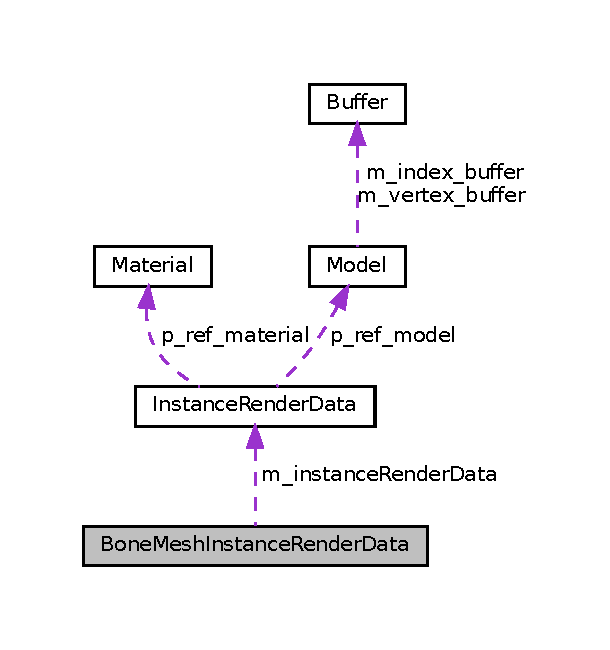
\includegraphics[width=293pt]{structBoneMeshInstanceRenderData__coll__graph}
\end{center}
\end{figure}
\subsection*{Public Attributes}
\begin{DoxyCompactItemize}
\item 
\mbox{\Hypertarget{structBoneMeshInstanceRenderData_aece2eb77387fb00b70aa51bd97fa5f6b}\label{structBoneMeshInstanceRenderData_aece2eb77387fb00b70aa51bd97fa5f6b}} 
\hyperlink{structInstanceRenderData}{Instance\+Render\+Data} {\bfseries m\+\_\+instance\+Render\+Data}
\item 
\mbox{\Hypertarget{structBoneMeshInstanceRenderData_abf865b22020ad64a00f2fb32028c3262}\label{structBoneMeshInstanceRenderData_abf865b22020ad64a00f2fb32028c3262}} 
Bone\+Transformations\+List $\ast$ {\bfseries m\+\_\+p\+Bone\+Transformations\+List}
\end{DoxyCompactItemize}


The documentation for this struct was generated from the following file\+:\begin{DoxyCompactItemize}
\item 
Graphics/Instance\+Render\+Data.\+h\end{DoxyCompactItemize}

\hypertarget{structBoneTransformsUniformData}{}\section{Bone\+Transforms\+Uniform\+Data Struct Reference}
\label{structBoneTransformsUniformData}\index{Bone\+Transforms\+Uniform\+Data@{Bone\+Transforms\+Uniform\+Data}}
\subsection*{Public Attributes}
\begin{DoxyCompactItemize}
\item 
\mbox{\Hypertarget{structBoneTransformsUniformData_a829bcf868620ce499045a9f47c487c99}\label{structBoneTransformsUniformData_a829bcf868620ce499045a9f47c487c99}} 
float4x4 {\bfseries Bone\+Transforms} \mbox{[}M\+A\+X\+\_\+\+B\+O\+N\+E\+\_\+\+C\+O\+U\+NT\mbox{]}
\end{DoxyCompactItemize}


The documentation for this struct was generated from the following file\+:\begin{DoxyCompactItemize}
\item 
Shaders/Shading.\+h\end{DoxyCompactItemize}

\hypertarget{structBoneVertexData}{}\section{Bone\+Vertex\+Data Struct Reference}
\label{structBoneVertexData}\index{Bone\+Vertex\+Data@{Bone\+Vertex\+Data}}
\subsection*{Public Attributes}
\begin{DoxyCompactItemize}
\item 
\mbox{\Hypertarget{structBoneVertexData_ab3244a27730090f33a966f117796a15c}\label{structBoneVertexData_ab3244a27730090f33a966f117796a15c}} 
int32\+\_\+t {\bfseries m\+\_\+bone\+Indices} \mbox{[}4\mbox{]}
\item 
\mbox{\Hypertarget{structBoneVertexData_ab8de7e288e7068d116df550470c41c14}\label{structBoneVertexData_ab8de7e288e7068d116df550470c41c14}} 
float {\bfseries m\+\_\+bone\+Weights} \mbox{[}4\mbox{]}
\end{DoxyCompactItemize}


The documentation for this struct was generated from the following file\+:\begin{DoxyCompactItemize}
\item 
Animation/Anim\+Model.\+h\end{DoxyCompactItemize}

\hypertarget{classBRDFLookupTexturePass}{}\section{B\+R\+D\+F\+Lookup\+Texture\+Pass Class Reference}
\label{classBRDFLookupTexturePass}\index{B\+R\+D\+F\+Lookup\+Texture\+Pass@{B\+R\+D\+F\+Lookup\+Texture\+Pass}}
\subsection*{Public Member Functions}
\begin{DoxyCompactItemize}
\item 
\mbox{\Hypertarget{classBRDFLookupTexturePass_a0b442fac37fde6e275f40df0eb1e0fc6}\label{classBRDFLookupTexturePass_a0b442fac37fde6e275f40df0eb1e0fc6}} 
{\bfseries B\+R\+D\+F\+Lookup\+Texture\+Pass} (\hyperlink{classAppRenderer}{App\+Renderer} $\ast$app\+Renderer)
\item 
\mbox{\Hypertarget{classBRDFLookupTexturePass_a54e0d191bd57d642ff039ed60521da6f}\label{classBRDFLookupTexturePass_a54e0d191bd57d642ff039ed60521da6f}} 
void {\bfseries Render} (\hyperlink{classTexture}{Texture} $\ast$brdf\+\_\+lut\+\_\+texture)
\item 
\mbox{\Hypertarget{classBRDFLookupTexturePass_a2449e85dba714e6305b68973d2a4105a}\label{classBRDFLookupTexturePass_a2449e85dba714e6305b68973d2a4105a}} 
void {\bfseries Initialize} (\hyperlink{classDXRenderer}{D\+X\+Renderer} $\ast$dxrenderer)
\item 
\mbox{\Hypertarget{classBRDFLookupTexturePass_a8a20b058ccfcf92afab17f199a74e2a1}\label{classBRDFLookupTexturePass_a8a20b058ccfcf92afab17f199a74e2a1}} 
void {\bfseries Release} ()
\end{DoxyCompactItemize}


The documentation for this class was generated from the following files\+:\begin{DoxyCompactItemize}
\item 
Graphics/\+I\+B\+L/B\+R\+D\+F\+Lookup\+Texture\+Pass.\+h\item 
Graphics/\+I\+B\+L/B\+R\+D\+F\+Lookup\+Texture\+Pass.\+cpp\end{DoxyCompactItemize}

\hypertarget{classBuffer}{}\section{Buffer Class Reference}
\label{classBuffer}\index{Buffer@{Buffer}}
\subsection*{Public Member Functions}
\begin{DoxyCompactItemize}
\item 
\mbox{\Hypertarget{classBuffer_aaeb3b3f04ba947f13ca177c33605a384}\label{classBuffer_aaeb3b3f04ba947f13ca177c33605a384}} 
void {\bfseries Release} ()
\end{DoxyCompactItemize}
\subsection*{Friends}
\begin{DoxyCompactItemize}
\item 
\mbox{\Hypertarget{classBuffer_a871268c492209c5a9db9dc2db99f4d04}\label{classBuffer_a871268c492209c5a9db9dc2db99f4d04}} 
class {\bfseries D\+X\+Resource\+Loader}
\item 
\mbox{\Hypertarget{classBuffer_a14ab6f966322dccbf6597d0c82bf48c6}\label{classBuffer_a14ab6f966322dccbf6597d0c82bf48c6}} 
class {\bfseries D\+X\+Renderer}
\end{DoxyCompactItemize}


The documentation for this class was generated from the following files\+:\begin{DoxyCompactItemize}
\item 
Graphics/Buffer.\+h\item 
Graphics/Buffer.\+cpp\end{DoxyCompactItemize}

\hypertarget{structBufferDesc}{}\section{Buffer\+Desc Struct Reference}
\label{structBufferDesc}\index{Buffer\+Desc@{Buffer\+Desc}}
\subsection*{Public Attributes}
\begin{DoxyCompactItemize}
\item 
\mbox{\Hypertarget{structBufferDesc_aec5b4aa274b3e1c8e1ca407cf1cbc0af}\label{structBufferDesc_aec5b4aa274b3e1c8e1ca407cf1cbc0af}} 
uint32\+\_\+t {\bfseries m\+\_\+bind\+Flags}
\item 
\mbox{\Hypertarget{structBufferDesc_a608b3397ef0ac6c5172189cc42fc676b}\label{structBufferDesc_a608b3397ef0ac6c5172189cc42fc676b}} 
Usage\+\_\+\+Type {\bfseries m\+\_\+usage\+Type}
\item 
\mbox{\Hypertarget{structBufferDesc_a6ee4fbb68f0351850bd71c8185c000f9}\label{structBufferDesc_a6ee4fbb68f0351850bd71c8185c000f9}} 
C\+P\+U\+\_\+\+Access\+\_\+\+Type {\bfseries m\+\_\+cpu\+Access\+Type}
\item 
\mbox{\Hypertarget{structBufferDesc_af60d327f66eb6cd4e56255823cf58e6d}\label{structBufferDesc_af60d327f66eb6cd4e56255823cf58e6d}} 
Misc\+\_\+\+Flags {\bfseries m\+\_\+misc\+Flags}
\item 
\mbox{\Hypertarget{structBufferDesc_af5381dcb6c0c6b6b0f1bcaeb1ae18642}\label{structBufferDesc_af5381dcb6c0c6b6b0f1bcaeb1ae18642}} 
uint32\+\_\+t {\bfseries m\+\_\+vertex\+Stride}
\item 
\mbox{\Hypertarget{structBufferDesc_a76eb0fc282e0aff2eee731ea7ce2e461}\label{structBufferDesc_a76eb0fc282e0aff2eee731ea7ce2e461}} 
Index\+Type {\bfseries m\+\_\+index\+Type}
\item 
\mbox{\Hypertarget{structBufferDesc_acab9cd5599ccaec586415deb8353f62f}\label{structBufferDesc_acab9cd5599ccaec586415deb8353f62f}} 
uint32\+\_\+t {\bfseries m\+\_\+first\+Element}
\item 
\mbox{\Hypertarget{structBufferDesc_a3868b7e07063db3050199780fadf4e03}\label{structBufferDesc_a3868b7e07063db3050199780fadf4e03}} 
uint32\+\_\+t {\bfseries m\+\_\+element\+Count}
\item 
\mbox{\Hypertarget{structBufferDesc_aeb86e6e1e64c56ade38ec6cd1887b057}\label{structBufferDesc_aeb86e6e1e64c56ade38ec6cd1887b057}} 
uint32\+\_\+t {\bfseries m\+\_\+structure\+Stride}
\item 
\mbox{\Hypertarget{structBufferDesc_af82649bab7d3e365f68bd95bc02a4f28}\label{structBufferDesc_af82649bab7d3e365f68bd95bc02a4f28}} 
D\+X\+G\+I\+\_\+\+F\+O\+R\+M\+AT {\bfseries m\+\_\+buffer\+Format}
\item 
\mbox{\Hypertarget{structBufferDesc_a19a8209c8dfe49f609d1b515d477ec34}\label{structBufferDesc_a19a8209c8dfe49f609d1b515d477ec34}} 
std\+::string {\bfseries m\+\_\+debug\+Name}
\end{DoxyCompactItemize}


The documentation for this struct was generated from the following file\+:\begin{DoxyCompactItemize}
\item 
Graphics/Buffer.\+h\end{DoxyCompactItemize}

\hypertarget{structBufferLoadDesc}{}\section{Buffer\+Load\+Desc Struct Reference}
\label{structBufferLoadDesc}\index{Buffer\+Load\+Desc@{Buffer\+Load\+Desc}}


Collaboration diagram for Buffer\+Load\+Desc\+:\nopagebreak
\begin{figure}[H]
\begin{center}
\leavevmode
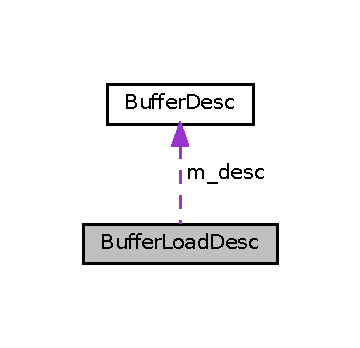
\includegraphics[width=173pt]{structBufferLoadDesc__coll__graph}
\end{center}
\end{figure}
\subsection*{Public Member Functions}
\begin{DoxyCompactItemize}
\item 
\mbox{\Hypertarget{structBufferLoadDesc_a2d469bae2e844f9b0839702622ccf6fc}\label{structBufferLoadDesc_a2d469bae2e844f9b0839702622ccf6fc}} 
{\bfseries Buffer\+Load\+Desc} (const void $\ast$raw\+\_\+data=nullptr)
\end{DoxyCompactItemize}
\subsection*{Public Attributes}
\begin{DoxyCompactItemize}
\item 
\mbox{\Hypertarget{structBufferLoadDesc_a37d56783b4af4e75eb61cf820d7520da}\label{structBufferLoadDesc_a37d56783b4af4e75eb61cf820d7520da}} 
\hyperlink{structBufferDesc}{Buffer\+Desc} {\bfseries m\+\_\+desc}
\item 
\mbox{\Hypertarget{structBufferLoadDesc_ae67e17527abc39c6045571fe8ea7fc87}\label{structBufferLoadDesc_ae67e17527abc39c6045571fe8ea7fc87}} 
const void $\ast$ {\bfseries m\+\_\+raw\+Data}
\item 
\mbox{\Hypertarget{structBufferLoadDesc_a12152f6fd71fb0ff2e4743d1424c143d}\label{structBufferLoadDesc_a12152f6fd71fb0ff2e4743d1424c143d}} 
uint32\+\_\+t {\bfseries m\+\_\+size}
\end{DoxyCompactItemize}


The documentation for this struct was generated from the following file\+:\begin{DoxyCompactItemize}
\item 
Graphics/Buffer.\+h\end{DoxyCompactItemize}

\hypertarget{structBufferUpdateDesc}{}\section{Buffer\+Update\+Desc Struct Reference}
\label{structBufferUpdateDesc}\index{Buffer\+Update\+Desc@{Buffer\+Update\+Desc}}


Collaboration diagram for Buffer\+Update\+Desc\+:
\nopagebreak
\begin{figure}[H]
\begin{center}
\leavevmode
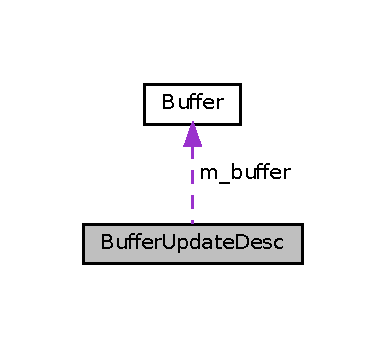
\includegraphics[width=185pt]{structBufferUpdateDesc__coll__graph}
\end{center}
\end{figure}
\subsection*{Public Attributes}
\begin{DoxyCompactItemize}
\item 
\mbox{\Hypertarget{structBufferUpdateDesc_ade220b235f3023166d572729aaca6b39}\label{structBufferUpdateDesc_ade220b235f3023166d572729aaca6b39}} 
\hyperlink{classBuffer}{Buffer} $\ast$ {\bfseries m\+\_\+buffer}
\item 
\mbox{\Hypertarget{structBufferUpdateDesc_a91446ea04ab679e342aeec70e8f1d639}\label{structBufferUpdateDesc_a91446ea04ab679e342aeec70e8f1d639}} 
const void $\ast$ {\bfseries m\+\_\+p\+Source}
\item 
\mbox{\Hypertarget{structBufferUpdateDesc_a45260587c314ad5b3f13d12fc319d627}\label{structBufferUpdateDesc_a45260587c314ad5b3f13d12fc319d627}} 
uint32\+\_\+t {\bfseries m\+\_\+source\+Offset}
\item 
\mbox{\Hypertarget{structBufferUpdateDesc_a0c7a966925823826f53fe61fb11970a4}\label{structBufferUpdateDesc_a0c7a966925823826f53fe61fb11970a4}} 
uint32\+\_\+t {\bfseries m\+\_\+dest\+Offset}
\item 
\mbox{\Hypertarget{structBufferUpdateDesc_a739cfc54bbe93d4ec27ce7ddae82c7df}\label{structBufferUpdateDesc_a739cfc54bbe93d4ec27ce7ddae82c7df}} 
uint32\+\_\+t {\bfseries m\+\_\+size}
\end{DoxyCompactItemize}


The documentation for this struct was generated from the following file\+:\begin{DoxyCompactItemize}
\item 
Graphics/Buffer.\+h\end{DoxyCompactItemize}

\hypertarget{classCamera}{}\section{Camera Class Reference}
\label{classCamera}\index{Camera@{Camera}}


The public interface for 3D \hyperlink{classCamera}{Camera}.  




{\ttfamily \#include $<$Camera.\+h$>$}

\subsection*{Public Member Functions}
\begin{DoxyCompactItemize}
\item 
\mbox{\Hypertarget{classCamera_ad6ec69dd0867f0c3eea93421977af1af}\label{classCamera_ad6ec69dd0867f0c3eea93421977af1af}} 
{\bfseries Camera} (const \hyperlink{classCamera}{Camera} \&lhs)
\item 
\mbox{\Hypertarget{classCamera_ab1abbdc02f4eab52c9a5af67b4c200d7}\label{classCamera_ab1abbdc02f4eab52c9a5af67b4c200d7}} 
{\bfseries Camera} (float fov, float near\+Val, float far\+V\+Al, const Vector3 \&position)
\item 
void \hyperlink{classCamera_aea06aa6e65a320393f703378f46ba40f}{Set\+F\+OV} (float fov)
\begin{DoxyCompactList}\small\item\em Set the field of view (degree) \end{DoxyCompactList}\item 
void \hyperlink{classCamera_a57e39ce60794095afebda3d38b681fe9}{Increase\+F\+OV} (float fov)
\begin{DoxyCompactList}\small\item\em Increase the field of view (degree) \end{DoxyCompactList}\item 
void \hyperlink{classCamera_a0d7a72fc6b726a97bc2babf0bb09550e}{Decrease\+F\+OV} (float fov)
\begin{DoxyCompactList}\small\item\em Decrease the field of view (degree) \end{DoxyCompactList}\item 
float \hyperlink{classCamera_aacd8360b4fb585a3cdc44ea83e55fc36}{Get\+F\+OV} () const
\begin{DoxyCompactList}\small\item\em Get field of view. \end{DoxyCompactList}\item 
void \hyperlink{classCamera_a8144951dd9ddd5557176e677fdfac282}{Set\+Aspect\+Ratio} (size\+\_\+t width, size\+\_\+t height)
\begin{DoxyCompactList}\small\item\em Set the Aspect Ratio of the \hyperlink{classCamera}{Camera}. \end{DoxyCompactList}\item 
void \hyperlink{classCamera_a8757dff50ae7715a05cb24596e008021}{Set\+Projection\+Type} (Camera\+Projection\+Type projection\+Type)
\begin{DoxyCompactList}\small\item\em Set the Projection Type. There is perspective, orthographic, and orthographic viewport. \end{DoxyCompactList}\item 
uint32\+\_\+t \hyperlink{classCamera_aa2ae7a317fca3bf2278d83317251860d}{Get\+Camera\+Render\+Object\+Type} () const
\begin{DoxyCompactList}\small\item\em Get the render type. \hyperlink{classCamera}{Camera} can render either 3D mesh, ui, or both. \end{DoxyCompactList}\item 
void \hyperlink{classCamera_a084b1b5028ff915b0f30734c4fcb7ac7}{Set\+Camera\+Render\+Object\+Type} (uint32\+\_\+t render\+Object\+Type)
\begin{DoxyCompactList}\small\item\em Set the render type. \hyperlink{classCamera}{Camera} can render either 3D mesh, ui, or both. \end{DoxyCompactList}\item 
void \hyperlink{classCamera_a83ffec8a5dfac0fa1ca1ea6388035dca}{Set\+Camera\+Position} (float x, float y, float z)
\begin{DoxyCompactList}\small\item\em Set the \hyperlink{classCamera}{Camera} Position. \end{DoxyCompactList}\item 
void \hyperlink{classCamera_a3a2df84800e210c35c8282b0f1022dac}{Set\+Camera\+Position} (const Vector3 \&new\+\_\+position)
\begin{DoxyCompactList}\small\item\em Set the \hyperlink{classCamera}{Camera} Position. \end{DoxyCompactList}\item 
void \hyperlink{classCamera_a71d00531ecb1f5cd9f3402bc3f1a4f30}{Set\+Look} (Vector3 look)
\begin{DoxyCompactList}\small\item\em Set the \hyperlink{classCamera}{Camera} look direction. \end{DoxyCompactList}\item 
void \hyperlink{classCamera_a148acfe88ccb73ba5b658cd2e19ee244}{Set\+Camera\+Rotation} (const Matrix \&new\+\_\+position)
\begin{DoxyCompactList}\small\item\em Set the \hyperlink{classCamera}{Camera} Rotation. \end{DoxyCompactList}\item 
Vector2 \hyperlink{classCamera_a601c02931f32a0909bba512fb26a7b0c}{Get\+Width\+Height} () const
\begin{DoxyCompactList}\small\item\em Get the screen width \& screen height that is associated with this camera. \end{DoxyCompactList}\item 
Vector3 \hyperlink{classCamera_a9378bf4ae942a64e0bbda67a79e57922}{Get\+Camera\+Position} () const
\begin{DoxyCompactList}\small\item\em Get the \hyperlink{classCamera}{Camera} Position. \end{DoxyCompactList}\item 
const Vector3 \& \hyperlink{classCamera_a2b34df2f0303bac1ed652bc3186e5a98}{Get\+Forward} () const
\begin{DoxyCompactList}\small\item\em Get \hyperlink{classCamera}{Camera} look at vector/forward vector. \end{DoxyCompactList}\item 
const Vector3 \& \hyperlink{classCamera_afd3c91fa693b8a6fb74d2e4708f3aae2}{Get\+Right} () const
\begin{DoxyCompactList}\small\item\em Get \hyperlink{classCamera}{Camera} Right vector. \end{DoxyCompactList}\item 
const Vector3 \& \hyperlink{classCamera_a0d14fb92d976926e8fcec4409c1e2812}{Get\+Up} () const
\begin{DoxyCompactList}\small\item\em Get \hyperlink{classCamera}{Camera} Up vector. \end{DoxyCompactList}\item 
\mbox{\Hypertarget{classCamera_aa46f58b32270a571ab56dde4caca46db}\label{classCamera_aa46f58b32270a571ab56dde4caca46db}} 
void {\bfseries Reset} ()
\item 
const Matrix \& \hyperlink{classCamera_ae56a0f8c9aa2d4eead91fe342159b1e5}{Get\+View\+Matrix} () const
\begin{DoxyCompactList}\small\item\em Get the View Matrix. \end{DoxyCompactList}\item 
const Matrix \& \hyperlink{classCamera_a7af480f3ec57bf981cd00b202aa0ff13}{Get\+Inv\+View\+Matrix} () const
\begin{DoxyCompactList}\small\item\em Get the Inverse View Matrix. \end{DoxyCompactList}\item 
Matrix \hyperlink{classCamera_ad9cd52470afe2f8a0e7a651f4592ee3c}{Get\+Inv\+View\+Matrix\+Copy} () const
\begin{DoxyCompactList}\small\item\em Get the copy of Inverse View Matrix. \end{DoxyCompactList}\item 
const Matrix \& \hyperlink{classCamera_a51e9a67637aeb424e1e173eae22d23c1}{Get\+Projection\+Matrix} () const
\begin{DoxyCompactList}\small\item\em Get the Projection Matrix. \end{DoxyCompactList}\item 
const Matrix \& \hyperlink{classCamera_a8c4b6ade261f29d41517bd1674404ccc}{Get\+Inv\+Projection\+Matrix} () const
\begin{DoxyCompactList}\small\item\em Get the Inverse Projection Matrix. \end{DoxyCompactList}\item 
const Matrix \& \hyperlink{classCamera_a2b52161705059c0f182d4d0b62808211}{Get\+View\+Projection\+Matrix} () const
\begin{DoxyCompactList}\small\item\em Get the View Projection Matrix. \end{DoxyCompactList}\item 
const Matrix \& \hyperlink{classCamera_a00cfc3d1d31e179df4d02b3878da75bd}{Get\+Inv\+View\+Projection\+Matrix} () const
\begin{DoxyCompactList}\small\item\em Get the Inverse View Projection Matrix. \end{DoxyCompactList}\item 
\mbox{\Hypertarget{classCamera_a69369efae2a33da50510cc8c43c58bc5}\label{classCamera_a69369efae2a33da50510cc8c43c58bc5}} 
void {\bfseries Update\+View\+Matrix} ()
\item 
\mbox{\Hypertarget{classCamera_a619c58dc226f1489502c9ed33ad87323}\label{classCamera_a619c58dc226f1489502c9ed33ad87323}} 
void {\bfseries Update\+Projection\+Matrix} ()
\item 
\mbox{\Hypertarget{classCamera_a44f25453a2a87f32d325f88bf3686add}\label{classCamera_a44f25453a2a87f32d325f88bf3686add}} 
void {\bfseries Update\+View\+Projection\+Matrix} ()
\item 
\mbox{\Hypertarget{classCamera_a863a3a0132d64395c04a418e0f6174a3}\label{classCamera_a863a3a0132d64395c04a418e0f6174a3}} 
size\+\_\+t {\bfseries Get\+Id} ()
\item 
\mbox{\Hypertarget{classCamera_a1b4079998b211f9bed22323564e2f875}\label{classCamera_a1b4079998b211f9bed22323564e2f875}} 
std\+::string {\bfseries Get\+Camera\+Name} () const
\item 
int32\+\_\+t \hyperlink{classCamera_a6c981b26fc23315fcc7e6776d7dee4ae}{Get\+Z\+Order} () const
\begin{DoxyCompactList}\small\item\em Get \hyperlink{classCamera}{Camera} Z Order. The higher the Z order means the render target of the \hyperlink{classCamera}{Camera} will be more on the top of the window screen. \end{DoxyCompactList}\item 
const Vector4 \& \hyperlink{classCamera_a055588d001b70381c0d5eaccdf9f7ece}{Get\+Viewport\+Render\+Information} () const
\begin{DoxyCompactList}\small\item\em Get the Viewport Render Information. This describe the size of the render target a camera should have. \end{DoxyCompactList}\item 
size\+\_\+t \hyperlink{classCamera_aa2812325bada4a9c1955f005c125b313}{Get\+Screen\+Width} () const
\begin{DoxyCompactList}\small\item\em Get the Screen Width. \end{DoxyCompactList}\item 
size\+\_\+t \hyperlink{classCamera_ad6bf28a11aa95a86497ad1e0d476d95b}{Get\+Screen\+Height} () const
\begin{DoxyCompactList}\small\item\em Get the Screen Height. \end{DoxyCompactList}\item 
void \hyperlink{classCamera_aa4d72b13e178899c2bdb68652a8fd10a}{Set\+Orthographic\+Width} (size\+\_\+t width)
\begin{DoxyCompactList}\small\item\em Set the Orthographic Width. Only for orthographic camera. \end{DoxyCompactList}\item 
void \hyperlink{classCamera_a59239b01b73f2e6aeb482b32831aba2b}{Set\+Orthographic\+Height} (size\+\_\+t height)
\begin{DoxyCompactList}\small\item\em Set the Orthographic Height. Only for orthographic camera. \end{DoxyCompactList}\item 
size\+\_\+t \hyperlink{classCamera_a247797f293fc7e2aa7529c3ad0ea4739}{Get\+Orthographic\+Width} () const
\begin{DoxyCompactList}\small\item\em Get the Orthographic Width. Only for orthographic camera. \end{DoxyCompactList}\item 
size\+\_\+t \hyperlink{classCamera_a12110e195967b52900768e4e008c7d63}{Get\+Orthographic\+Height} () const
\begin{DoxyCompactList}\small\item\em Get the Orthographic Height. Only for orthographic camera. \end{DoxyCompactList}\end{DoxyCompactItemize}
\subsection*{Friends}
\begin{DoxyCompactItemize}
\item 
\mbox{\Hypertarget{classCamera_ad7590dd71ff942ecb6f2926afddaafbe}\label{classCamera_ad7590dd71ff942ecb6f2926afddaafbe}} 
class {\bfseries F\+P\+S\+Camera\+System}
\item 
\mbox{\Hypertarget{classCamera_ae834a5e62eff7d0adb1092a0693388f7}\label{classCamera_ae834a5e62eff7d0adb1092a0693388f7}} 
class {\bfseries Camera\+Component}
\end{DoxyCompactItemize}


\subsection{Detailed Description}
The public interface for 3D \hyperlink{classCamera}{Camera}. 

\subsection{Member Function Documentation}
\mbox{\Hypertarget{classCamera_a0d7a72fc6b726a97bc2babf0bb09550e}\label{classCamera_a0d7a72fc6b726a97bc2babf0bb09550e}} 
\index{Camera@{Camera}!Decrease\+F\+OV@{Decrease\+F\+OV}}
\index{Decrease\+F\+OV@{Decrease\+F\+OV}!Camera@{Camera}}
\subsubsection{\texorpdfstring{Decrease\+F\+O\+V()}{DecreaseFOV()}}
{\footnotesize\ttfamily void Camera\+::\+Decrease\+F\+OV (\begin{DoxyParamCaption}\item[{float}]{fov }\end{DoxyParamCaption})}



Decrease the field of view (degree) 


\begin{DoxyParams}{Parameters}
{\em fov} & \\
\hline
\end{DoxyParams}
\mbox{\Hypertarget{classCamera_a9378bf4ae942a64e0bbda67a79e57922}\label{classCamera_a9378bf4ae942a64e0bbda67a79e57922}} 
\index{Camera@{Camera}!Get\+Camera\+Position@{Get\+Camera\+Position}}
\index{Get\+Camera\+Position@{Get\+Camera\+Position}!Camera@{Camera}}
\subsubsection{\texorpdfstring{Get\+Camera\+Position()}{GetCameraPosition()}}
{\footnotesize\ttfamily Vector3 Camera\+::\+Get\+Camera\+Position (\begin{DoxyParamCaption}{ }\end{DoxyParamCaption}) const}



Get the \hyperlink{classCamera}{Camera} Position. 

\begin{DoxyReturn}{Returns}
Vector3 
\end{DoxyReturn}
\mbox{\Hypertarget{classCamera_aa2ae7a317fca3bf2278d83317251860d}\label{classCamera_aa2ae7a317fca3bf2278d83317251860d}} 
\index{Camera@{Camera}!Get\+Camera\+Render\+Object\+Type@{Get\+Camera\+Render\+Object\+Type}}
\index{Get\+Camera\+Render\+Object\+Type@{Get\+Camera\+Render\+Object\+Type}!Camera@{Camera}}
\subsubsection{\texorpdfstring{Get\+Camera\+Render\+Object\+Type()}{GetCameraRenderObjectType()}}
{\footnotesize\ttfamily uint32\+\_\+t Camera\+::\+Get\+Camera\+Render\+Object\+Type (\begin{DoxyParamCaption}{ }\end{DoxyParamCaption}) const}



Get the render type. \hyperlink{classCamera}{Camera} can render either 3D mesh, ui, or both. 

\begin{DoxyReturn}{Returns}
uint32\+\_\+t 
\end{DoxyReturn}
\mbox{\Hypertarget{classCamera_a2b34df2f0303bac1ed652bc3186e5a98}\label{classCamera_a2b34df2f0303bac1ed652bc3186e5a98}} 
\index{Camera@{Camera}!Get\+Forward@{Get\+Forward}}
\index{Get\+Forward@{Get\+Forward}!Camera@{Camera}}
\subsubsection{\texorpdfstring{Get\+Forward()}{GetForward()}}
{\footnotesize\ttfamily const Vector3 \& Camera\+::\+Get\+Forward (\begin{DoxyParamCaption}{ }\end{DoxyParamCaption}) const}



Get \hyperlink{classCamera}{Camera} look at vector/forward vector. 

\begin{DoxyReturn}{Returns}
const Vector3\& 
\end{DoxyReturn}
\mbox{\Hypertarget{classCamera_aacd8360b4fb585a3cdc44ea83e55fc36}\label{classCamera_aacd8360b4fb585a3cdc44ea83e55fc36}} 
\index{Camera@{Camera}!Get\+F\+OV@{Get\+F\+OV}}
\index{Get\+F\+OV@{Get\+F\+OV}!Camera@{Camera}}
\subsubsection{\texorpdfstring{Get\+F\+O\+V()}{GetFOV()}}
{\footnotesize\ttfamily float Camera\+::\+Get\+F\+OV (\begin{DoxyParamCaption}{ }\end{DoxyParamCaption}) const}



Get field of view. 

\begin{DoxyReturn}{Returns}
float 
\end{DoxyReturn}
\mbox{\Hypertarget{classCamera_a8c4b6ade261f29d41517bd1674404ccc}\label{classCamera_a8c4b6ade261f29d41517bd1674404ccc}} 
\index{Camera@{Camera}!Get\+Inv\+Projection\+Matrix@{Get\+Inv\+Projection\+Matrix}}
\index{Get\+Inv\+Projection\+Matrix@{Get\+Inv\+Projection\+Matrix}!Camera@{Camera}}
\subsubsection{\texorpdfstring{Get\+Inv\+Projection\+Matrix()}{GetInvProjectionMatrix()}}
{\footnotesize\ttfamily const Matrix\& Camera\+::\+Get\+Inv\+Projection\+Matrix (\begin{DoxyParamCaption}{ }\end{DoxyParamCaption}) const\hspace{0.3cm}{\ttfamily [inline]}}



Get the Inverse Projection Matrix. 

\begin{DoxyReturn}{Returns}
const Matrix\& 
\end{DoxyReturn}
\mbox{\Hypertarget{classCamera_a7af480f3ec57bf981cd00b202aa0ff13}\label{classCamera_a7af480f3ec57bf981cd00b202aa0ff13}} 
\index{Camera@{Camera}!Get\+Inv\+View\+Matrix@{Get\+Inv\+View\+Matrix}}
\index{Get\+Inv\+View\+Matrix@{Get\+Inv\+View\+Matrix}!Camera@{Camera}}
\subsubsection{\texorpdfstring{Get\+Inv\+View\+Matrix()}{GetInvViewMatrix()}}
{\footnotesize\ttfamily const Matrix\& Camera\+::\+Get\+Inv\+View\+Matrix (\begin{DoxyParamCaption}{ }\end{DoxyParamCaption}) const\hspace{0.3cm}{\ttfamily [inline]}}



Get the Inverse View Matrix. 

\begin{DoxyReturn}{Returns}
const Matrix\& 
\end{DoxyReturn}
\mbox{\Hypertarget{classCamera_ad9cd52470afe2f8a0e7a651f4592ee3c}\label{classCamera_ad9cd52470afe2f8a0e7a651f4592ee3c}} 
\index{Camera@{Camera}!Get\+Inv\+View\+Matrix\+Copy@{Get\+Inv\+View\+Matrix\+Copy}}
\index{Get\+Inv\+View\+Matrix\+Copy@{Get\+Inv\+View\+Matrix\+Copy}!Camera@{Camera}}
\subsubsection{\texorpdfstring{Get\+Inv\+View\+Matrix\+Copy()}{GetInvViewMatrixCopy()}}
{\footnotesize\ttfamily Matrix Camera\+::\+Get\+Inv\+View\+Matrix\+Copy (\begin{DoxyParamCaption}{ }\end{DoxyParamCaption}) const\hspace{0.3cm}{\ttfamily [inline]}}



Get the copy of Inverse View Matrix. 

\begin{DoxyReturn}{Returns}
const Matrix\& 
\end{DoxyReturn}
\mbox{\Hypertarget{classCamera_a00cfc3d1d31e179df4d02b3878da75bd}\label{classCamera_a00cfc3d1d31e179df4d02b3878da75bd}} 
\index{Camera@{Camera}!Get\+Inv\+View\+Projection\+Matrix@{Get\+Inv\+View\+Projection\+Matrix}}
\index{Get\+Inv\+View\+Projection\+Matrix@{Get\+Inv\+View\+Projection\+Matrix}!Camera@{Camera}}
\subsubsection{\texorpdfstring{Get\+Inv\+View\+Projection\+Matrix()}{GetInvViewProjectionMatrix()}}
{\footnotesize\ttfamily const Matrix\& Camera\+::\+Get\+Inv\+View\+Projection\+Matrix (\begin{DoxyParamCaption}{ }\end{DoxyParamCaption}) const\hspace{0.3cm}{\ttfamily [inline]}}



Get the Inverse View Projection Matrix. 

\begin{DoxyReturn}{Returns}
const Matrix\& 
\end{DoxyReturn}
\mbox{\Hypertarget{classCamera_a12110e195967b52900768e4e008c7d63}\label{classCamera_a12110e195967b52900768e4e008c7d63}} 
\index{Camera@{Camera}!Get\+Orthographic\+Height@{Get\+Orthographic\+Height}}
\index{Get\+Orthographic\+Height@{Get\+Orthographic\+Height}!Camera@{Camera}}
\subsubsection{\texorpdfstring{Get\+Orthographic\+Height()}{GetOrthographicHeight()}}
{\footnotesize\ttfamily size\+\_\+t Camera\+::\+Get\+Orthographic\+Height (\begin{DoxyParamCaption}{ }\end{DoxyParamCaption}) const}



Get the Orthographic Height. Only for orthographic camera. 

\begin{DoxyReturn}{Returns}
size\+\_\+t 
\end{DoxyReturn}
\mbox{\Hypertarget{classCamera_a247797f293fc7e2aa7529c3ad0ea4739}\label{classCamera_a247797f293fc7e2aa7529c3ad0ea4739}} 
\index{Camera@{Camera}!Get\+Orthographic\+Width@{Get\+Orthographic\+Width}}
\index{Get\+Orthographic\+Width@{Get\+Orthographic\+Width}!Camera@{Camera}}
\subsubsection{\texorpdfstring{Get\+Orthographic\+Width()}{GetOrthographicWidth()}}
{\footnotesize\ttfamily size\+\_\+t Camera\+::\+Get\+Orthographic\+Width (\begin{DoxyParamCaption}{ }\end{DoxyParamCaption}) const}



Get the Orthographic Width. Only for orthographic camera. 

\begin{DoxyReturn}{Returns}
size\+\_\+t 
\end{DoxyReturn}
\mbox{\Hypertarget{classCamera_a51e9a67637aeb424e1e173eae22d23c1}\label{classCamera_a51e9a67637aeb424e1e173eae22d23c1}} 
\index{Camera@{Camera}!Get\+Projection\+Matrix@{Get\+Projection\+Matrix}}
\index{Get\+Projection\+Matrix@{Get\+Projection\+Matrix}!Camera@{Camera}}
\subsubsection{\texorpdfstring{Get\+Projection\+Matrix()}{GetProjectionMatrix()}}
{\footnotesize\ttfamily const Matrix\& Camera\+::\+Get\+Projection\+Matrix (\begin{DoxyParamCaption}{ }\end{DoxyParamCaption}) const\hspace{0.3cm}{\ttfamily [inline]}}



Get the Projection Matrix. 

\begin{DoxyReturn}{Returns}
const Matrix\& 
\end{DoxyReturn}
\mbox{\Hypertarget{classCamera_afd3c91fa693b8a6fb74d2e4708f3aae2}\label{classCamera_afd3c91fa693b8a6fb74d2e4708f3aae2}} 
\index{Camera@{Camera}!Get\+Right@{Get\+Right}}
\index{Get\+Right@{Get\+Right}!Camera@{Camera}}
\subsubsection{\texorpdfstring{Get\+Right()}{GetRight()}}
{\footnotesize\ttfamily const Vector3 \& Camera\+::\+Get\+Right (\begin{DoxyParamCaption}{ }\end{DoxyParamCaption}) const}



Get \hyperlink{classCamera}{Camera} Right vector. 

\begin{DoxyReturn}{Returns}
const Vector3\& 
\end{DoxyReturn}
\mbox{\Hypertarget{classCamera_ad6bf28a11aa95a86497ad1e0d476d95b}\label{classCamera_ad6bf28a11aa95a86497ad1e0d476d95b}} 
\index{Camera@{Camera}!Get\+Screen\+Height@{Get\+Screen\+Height}}
\index{Get\+Screen\+Height@{Get\+Screen\+Height}!Camera@{Camera}}
\subsubsection{\texorpdfstring{Get\+Screen\+Height()}{GetScreenHeight()}}
{\footnotesize\ttfamily size\+\_\+t Camera\+::\+Get\+Screen\+Height (\begin{DoxyParamCaption}{ }\end{DoxyParamCaption}) const}



Get the Screen Height. 

\begin{DoxyReturn}{Returns}
size\+\_\+t 
\end{DoxyReturn}
\mbox{\Hypertarget{classCamera_aa2812325bada4a9c1955f005c125b313}\label{classCamera_aa2812325bada4a9c1955f005c125b313}} 
\index{Camera@{Camera}!Get\+Screen\+Width@{Get\+Screen\+Width}}
\index{Get\+Screen\+Width@{Get\+Screen\+Width}!Camera@{Camera}}
\subsubsection{\texorpdfstring{Get\+Screen\+Width()}{GetScreenWidth()}}
{\footnotesize\ttfamily size\+\_\+t Camera\+::\+Get\+Screen\+Width (\begin{DoxyParamCaption}{ }\end{DoxyParamCaption}) const}



Get the Screen Width. 

\begin{DoxyReturn}{Returns}
size\+\_\+t 
\end{DoxyReturn}
\mbox{\Hypertarget{classCamera_a0d14fb92d976926e8fcec4409c1e2812}\label{classCamera_a0d14fb92d976926e8fcec4409c1e2812}} 
\index{Camera@{Camera}!Get\+Up@{Get\+Up}}
\index{Get\+Up@{Get\+Up}!Camera@{Camera}}
\subsubsection{\texorpdfstring{Get\+Up()}{GetUp()}}
{\footnotesize\ttfamily const Vector3 \& Camera\+::\+Get\+Up (\begin{DoxyParamCaption}{ }\end{DoxyParamCaption}) const}



Get \hyperlink{classCamera}{Camera} Up vector. 

\begin{DoxyReturn}{Returns}
const Vector3\& 
\end{DoxyReturn}
\mbox{\Hypertarget{classCamera_ae56a0f8c9aa2d4eead91fe342159b1e5}\label{classCamera_ae56a0f8c9aa2d4eead91fe342159b1e5}} 
\index{Camera@{Camera}!Get\+View\+Matrix@{Get\+View\+Matrix}}
\index{Get\+View\+Matrix@{Get\+View\+Matrix}!Camera@{Camera}}
\subsubsection{\texorpdfstring{Get\+View\+Matrix()}{GetViewMatrix()}}
{\footnotesize\ttfamily const Matrix\& Camera\+::\+Get\+View\+Matrix (\begin{DoxyParamCaption}{ }\end{DoxyParamCaption}) const\hspace{0.3cm}{\ttfamily [inline]}}



Get the View Matrix. 

\begin{DoxyReturn}{Returns}
const Matrix\& 
\end{DoxyReturn}
\mbox{\Hypertarget{classCamera_a055588d001b70381c0d5eaccdf9f7ece}\label{classCamera_a055588d001b70381c0d5eaccdf9f7ece}} 
\index{Camera@{Camera}!Get\+Viewport\+Render\+Information@{Get\+Viewport\+Render\+Information}}
\index{Get\+Viewport\+Render\+Information@{Get\+Viewport\+Render\+Information}!Camera@{Camera}}
\subsubsection{\texorpdfstring{Get\+Viewport\+Render\+Information()}{GetViewportRenderInformation()}}
{\footnotesize\ttfamily const Vector4 \& Camera\+::\+Get\+Viewport\+Render\+Information (\begin{DoxyParamCaption}{ }\end{DoxyParamCaption}) const}



Get the Viewport Render Information. This describe the size of the render target a camera should have. 

\begin{DoxyReturn}{Returns}
const Vector4\& 
\end{DoxyReturn}
\mbox{\Hypertarget{classCamera_a2b52161705059c0f182d4d0b62808211}\label{classCamera_a2b52161705059c0f182d4d0b62808211}} 
\index{Camera@{Camera}!Get\+View\+Projection\+Matrix@{Get\+View\+Projection\+Matrix}}
\index{Get\+View\+Projection\+Matrix@{Get\+View\+Projection\+Matrix}!Camera@{Camera}}
\subsubsection{\texorpdfstring{Get\+View\+Projection\+Matrix()}{GetViewProjectionMatrix()}}
{\footnotesize\ttfamily const Matrix\& Camera\+::\+Get\+View\+Projection\+Matrix (\begin{DoxyParamCaption}{ }\end{DoxyParamCaption}) const\hspace{0.3cm}{\ttfamily [inline]}}



Get the View Projection Matrix. 

\begin{DoxyReturn}{Returns}
const Matrix\& 
\end{DoxyReturn}
\mbox{\Hypertarget{classCamera_a601c02931f32a0909bba512fb26a7b0c}\label{classCamera_a601c02931f32a0909bba512fb26a7b0c}} 
\index{Camera@{Camera}!Get\+Width\+Height@{Get\+Width\+Height}}
\index{Get\+Width\+Height@{Get\+Width\+Height}!Camera@{Camera}}
\subsubsection{\texorpdfstring{Get\+Width\+Height()}{GetWidthHeight()}}
{\footnotesize\ttfamily Vector2 Camera\+::\+Get\+Width\+Height (\begin{DoxyParamCaption}{ }\end{DoxyParamCaption}) const}



Get the screen width \& screen height that is associated with this camera. 

\begin{DoxyReturn}{Returns}
Vector2 
\end{DoxyReturn}
\mbox{\Hypertarget{classCamera_a6c981b26fc23315fcc7e6776d7dee4ae}\label{classCamera_a6c981b26fc23315fcc7e6776d7dee4ae}} 
\index{Camera@{Camera}!Get\+Z\+Order@{Get\+Z\+Order}}
\index{Get\+Z\+Order@{Get\+Z\+Order}!Camera@{Camera}}
\subsubsection{\texorpdfstring{Get\+Z\+Order()}{GetZOrder()}}
{\footnotesize\ttfamily int32\+\_\+t Camera\+::\+Get\+Z\+Order (\begin{DoxyParamCaption}{ }\end{DoxyParamCaption}) const}



Get \hyperlink{classCamera}{Camera} Z Order. The higher the Z order means the render target of the \hyperlink{classCamera}{Camera} will be more on the top of the window screen. 

\begin{DoxyReturn}{Returns}
int32\+\_\+t 
\end{DoxyReturn}
\mbox{\Hypertarget{classCamera_a57e39ce60794095afebda3d38b681fe9}\label{classCamera_a57e39ce60794095afebda3d38b681fe9}} 
\index{Camera@{Camera}!Increase\+F\+OV@{Increase\+F\+OV}}
\index{Increase\+F\+OV@{Increase\+F\+OV}!Camera@{Camera}}
\subsubsection{\texorpdfstring{Increase\+F\+O\+V()}{IncreaseFOV()}}
{\footnotesize\ttfamily void Camera\+::\+Increase\+F\+OV (\begin{DoxyParamCaption}\item[{float}]{fov }\end{DoxyParamCaption})}



Increase the field of view (degree) 


\begin{DoxyParams}{Parameters}
{\em fov} & \\
\hline
\end{DoxyParams}
\mbox{\Hypertarget{classCamera_a8144951dd9ddd5557176e677fdfac282}\label{classCamera_a8144951dd9ddd5557176e677fdfac282}} 
\index{Camera@{Camera}!Set\+Aspect\+Ratio@{Set\+Aspect\+Ratio}}
\index{Set\+Aspect\+Ratio@{Set\+Aspect\+Ratio}!Camera@{Camera}}
\subsubsection{\texorpdfstring{Set\+Aspect\+Ratio()}{SetAspectRatio()}}
{\footnotesize\ttfamily void Camera\+::\+Set\+Aspect\+Ratio (\begin{DoxyParamCaption}\item[{size\+\_\+t}]{width,  }\item[{size\+\_\+t}]{height }\end{DoxyParamCaption})}



Set the Aspect Ratio of the \hyperlink{classCamera}{Camera}. 


\begin{DoxyParams}{Parameters}
{\em width} & \\
\hline
{\em height} & \\
\hline
\end{DoxyParams}
\mbox{\Hypertarget{classCamera_a83ffec8a5dfac0fa1ca1ea6388035dca}\label{classCamera_a83ffec8a5dfac0fa1ca1ea6388035dca}} 
\index{Camera@{Camera}!Set\+Camera\+Position@{Set\+Camera\+Position}}
\index{Set\+Camera\+Position@{Set\+Camera\+Position}!Camera@{Camera}}
\subsubsection{\texorpdfstring{Set\+Camera\+Position()}{SetCameraPosition()}\hspace{0.1cm}{\footnotesize\ttfamily [1/2]}}
{\footnotesize\ttfamily void Camera\+::\+Set\+Camera\+Position (\begin{DoxyParamCaption}\item[{float}]{x,  }\item[{float}]{y,  }\item[{float}]{z }\end{DoxyParamCaption})}



Set the \hyperlink{classCamera}{Camera} Position. 


\begin{DoxyParams}{Parameters}
{\em x} & \\
\hline
{\em y} & \\
\hline
{\em z} & \\
\hline
\end{DoxyParams}
\mbox{\Hypertarget{classCamera_a3a2df84800e210c35c8282b0f1022dac}\label{classCamera_a3a2df84800e210c35c8282b0f1022dac}} 
\index{Camera@{Camera}!Set\+Camera\+Position@{Set\+Camera\+Position}}
\index{Set\+Camera\+Position@{Set\+Camera\+Position}!Camera@{Camera}}
\subsubsection{\texorpdfstring{Set\+Camera\+Position()}{SetCameraPosition()}\hspace{0.1cm}{\footnotesize\ttfamily [2/2]}}
{\footnotesize\ttfamily void Camera\+::\+Set\+Camera\+Position (\begin{DoxyParamCaption}\item[{const Vector3 \&}]{new\+\_\+position }\end{DoxyParamCaption})}



Set the \hyperlink{classCamera}{Camera} Position. 


\begin{DoxyParams}{Parameters}
{\em new\+\_\+position} & \\
\hline
\end{DoxyParams}
\mbox{\Hypertarget{classCamera_a084b1b5028ff915b0f30734c4fcb7ac7}\label{classCamera_a084b1b5028ff915b0f30734c4fcb7ac7}} 
\index{Camera@{Camera}!Set\+Camera\+Render\+Object\+Type@{Set\+Camera\+Render\+Object\+Type}}
\index{Set\+Camera\+Render\+Object\+Type@{Set\+Camera\+Render\+Object\+Type}!Camera@{Camera}}
\subsubsection{\texorpdfstring{Set\+Camera\+Render\+Object\+Type()}{SetCameraRenderObjectType()}}
{\footnotesize\ttfamily void Camera\+::\+Set\+Camera\+Render\+Object\+Type (\begin{DoxyParamCaption}\item[{uint32\+\_\+t}]{render\+Object\+Type }\end{DoxyParamCaption})}



Set the render type. \hyperlink{classCamera}{Camera} can render either 3D mesh, ui, or both. 


\begin{DoxyParams}{Parameters}
{\em render\+Object\+Type} & \\
\hline
\end{DoxyParams}
\mbox{\Hypertarget{classCamera_a148acfe88ccb73ba5b658cd2e19ee244}\label{classCamera_a148acfe88ccb73ba5b658cd2e19ee244}} 
\index{Camera@{Camera}!Set\+Camera\+Rotation@{Set\+Camera\+Rotation}}
\index{Set\+Camera\+Rotation@{Set\+Camera\+Rotation}!Camera@{Camera}}
\subsubsection{\texorpdfstring{Set\+Camera\+Rotation()}{SetCameraRotation()}}
{\footnotesize\ttfamily void Camera\+::\+Set\+Camera\+Rotation (\begin{DoxyParamCaption}\item[{const Matrix \&}]{new\+\_\+position }\end{DoxyParamCaption})}



Set the \hyperlink{classCamera}{Camera} Rotation. 


\begin{DoxyParams}{Parameters}
{\em new\+\_\+position} & \\
\hline
\end{DoxyParams}
\mbox{\Hypertarget{classCamera_aea06aa6e65a320393f703378f46ba40f}\label{classCamera_aea06aa6e65a320393f703378f46ba40f}} 
\index{Camera@{Camera}!Set\+F\+OV@{Set\+F\+OV}}
\index{Set\+F\+OV@{Set\+F\+OV}!Camera@{Camera}}
\subsubsection{\texorpdfstring{Set\+F\+O\+V()}{SetFOV()}}
{\footnotesize\ttfamily void Camera\+::\+Set\+F\+OV (\begin{DoxyParamCaption}\item[{float}]{fov }\end{DoxyParamCaption})}



Set the field of view (degree) 


\begin{DoxyParams}{Parameters}
{\em fov} & \\
\hline
\end{DoxyParams}
\mbox{\Hypertarget{classCamera_a71d00531ecb1f5cd9f3402bc3f1a4f30}\label{classCamera_a71d00531ecb1f5cd9f3402bc3f1a4f30}} 
\index{Camera@{Camera}!Set\+Look@{Set\+Look}}
\index{Set\+Look@{Set\+Look}!Camera@{Camera}}
\subsubsection{\texorpdfstring{Set\+Look()}{SetLook()}}
{\footnotesize\ttfamily void Camera\+::\+Set\+Look (\begin{DoxyParamCaption}\item[{Vector3}]{look }\end{DoxyParamCaption})}



Set the \hyperlink{classCamera}{Camera} look direction. 


\begin{DoxyParams}{Parameters}
{\em look} & \\
\hline
\end{DoxyParams}
\mbox{\Hypertarget{classCamera_a59239b01b73f2e6aeb482b32831aba2b}\label{classCamera_a59239b01b73f2e6aeb482b32831aba2b}} 
\index{Camera@{Camera}!Set\+Orthographic\+Height@{Set\+Orthographic\+Height}}
\index{Set\+Orthographic\+Height@{Set\+Orthographic\+Height}!Camera@{Camera}}
\subsubsection{\texorpdfstring{Set\+Orthographic\+Height()}{SetOrthographicHeight()}}
{\footnotesize\ttfamily void Camera\+::\+Set\+Orthographic\+Height (\begin{DoxyParamCaption}\item[{size\+\_\+t}]{height }\end{DoxyParamCaption})}



Set the Orthographic Height. Only for orthographic camera. 


\begin{DoxyParams}{Parameters}
{\em height} & \\
\hline
\end{DoxyParams}
\mbox{\Hypertarget{classCamera_aa4d72b13e178899c2bdb68652a8fd10a}\label{classCamera_aa4d72b13e178899c2bdb68652a8fd10a}} 
\index{Camera@{Camera}!Set\+Orthographic\+Width@{Set\+Orthographic\+Width}}
\index{Set\+Orthographic\+Width@{Set\+Orthographic\+Width}!Camera@{Camera}}
\subsubsection{\texorpdfstring{Set\+Orthographic\+Width()}{SetOrthographicWidth()}}
{\footnotesize\ttfamily void Camera\+::\+Set\+Orthographic\+Width (\begin{DoxyParamCaption}\item[{size\+\_\+t}]{width }\end{DoxyParamCaption})}



Set the Orthographic Width. Only for orthographic camera. 


\begin{DoxyParams}{Parameters}
{\em width} & \\
\hline
\end{DoxyParams}
\mbox{\Hypertarget{classCamera_a8757dff50ae7715a05cb24596e008021}\label{classCamera_a8757dff50ae7715a05cb24596e008021}} 
\index{Camera@{Camera}!Set\+Projection\+Type@{Set\+Projection\+Type}}
\index{Set\+Projection\+Type@{Set\+Projection\+Type}!Camera@{Camera}}
\subsubsection{\texorpdfstring{Set\+Projection\+Type()}{SetProjectionType()}}
{\footnotesize\ttfamily void Camera\+::\+Set\+Projection\+Type (\begin{DoxyParamCaption}\item[{Camera\+Projection\+Type}]{projection\+Type }\end{DoxyParamCaption})}



Set the Projection Type. There is perspective, orthographic, and orthographic viewport. 


\begin{DoxyParams}{Parameters}
{\em projection\+Type} & \\
\hline
\end{DoxyParams}


The documentation for this class was generated from the following files\+:\begin{DoxyCompactItemize}
\item 
Graphics/\hyperlink{Camera_8h}{Camera.\+h}\item 
Graphics/Camera.\+cpp\end{DoxyCompactItemize}

\hypertarget{structCameraCompNode}{}\section{Camera\+Comp\+Node Struct Reference}
\label{structCameraCompNode}\index{Camera\+Comp\+Node@{Camera\+Comp\+Node}}


Inheritance diagram for Camera\+Comp\+Node\+:\nopagebreak
\begin{figure}[H]
\begin{center}
\leavevmode
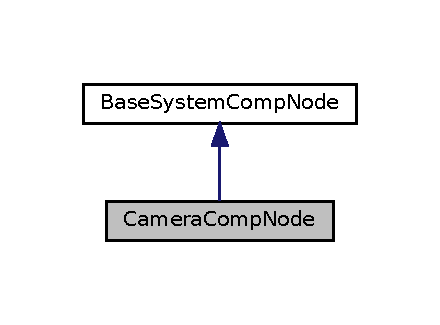
\includegraphics[width=211pt]{structCameraCompNode__inherit__graph}
\end{center}
\end{figure}


Collaboration diagram for Camera\+Comp\+Node\+:\nopagebreak
\begin{figure}[H]
\begin{center}
\leavevmode
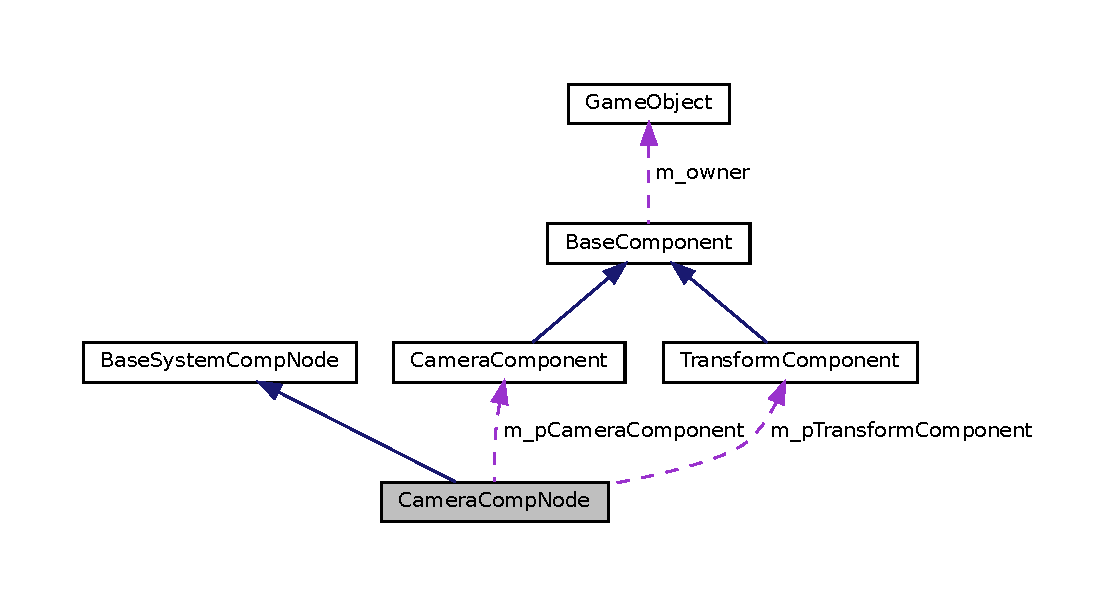
\includegraphics[width=350pt]{structCameraCompNode__coll__graph}
\end{center}
\end{figure}
\subsection*{Public Member Functions}
\begin{DoxyCompactItemize}
\item 
\mbox{\Hypertarget{structCameraCompNode_ad212f0250cd99dd43b73d9553c26cfda}\label{structCameraCompNode_ad212f0250cd99dd43b73d9553c26cfda}} 
{\bfseries Camera\+Comp\+Node} (\hyperlink{classTransformComponent}{Transform\+Component} $\ast$transform\+Comp, \hyperlink{classCameraComponent}{Camera\+Component} $\ast$camera\+Comp)
\end{DoxyCompactItemize}
\subsection*{Public Attributes}
\begin{DoxyCompactItemize}
\item 
\mbox{\Hypertarget{structCameraCompNode_a535902ba2bbef6190b4804952a623ee7}\label{structCameraCompNode_a535902ba2bbef6190b4804952a623ee7}} 
\hyperlink{classTransformComponent}{Transform\+Component} $\ast$ {\bfseries m\+\_\+p\+Transform\+Component}
\item 
\mbox{\Hypertarget{structCameraCompNode_ac45f3d84854086865468b82ea4df8c4d}\label{structCameraCompNode_ac45f3d84854086865468b82ea4df8c4d}} 
\hyperlink{classCameraComponent}{Camera\+Component} $\ast$ {\bfseries m\+\_\+p\+Camera\+Component}
\end{DoxyCompactItemize}


The documentation for this struct was generated from the following file\+:\begin{DoxyCompactItemize}
\item 
Systems/Camera\+System.\+h\end{DoxyCompactItemize}

\hypertarget{classCameraComponent}{}\section{Camera\+Component Class Reference}
\label{classCameraComponent}\index{Camera\+Component@{Camera\+Component}}


Inheritance diagram for Camera\+Component\+:
\nopagebreak
\begin{figure}[H]
\begin{center}
\leavevmode
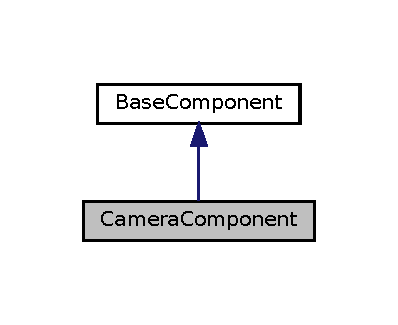
\includegraphics[width=191pt]{classCameraComponent__inherit__graph}
\end{center}
\end{figure}


Collaboration diagram for Camera\+Component\+:
\nopagebreak
\begin{figure}[H]
\begin{center}
\leavevmode
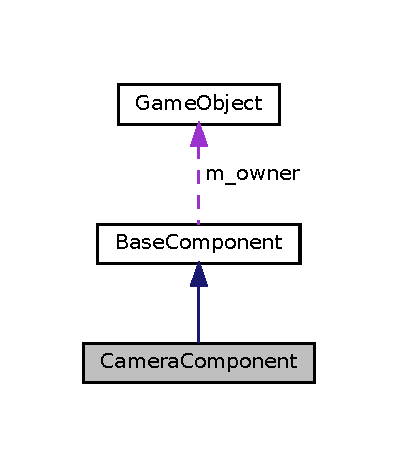
\includegraphics[width=191pt]{classCameraComponent__coll__graph}
\end{center}
\end{figure}
\subsection*{Public Member Functions}
\begin{DoxyCompactItemize}
\item 
\mbox{\Hypertarget{classCameraComponent_af29667817300732b1bf533ca8d1d3dee}\label{classCameraComponent_af29667817300732b1bf533ca8d1d3dee}} 
{\bfseries Camera\+Component} (\hyperlink{classGameObject}{Game\+Object} $\ast$owner)
\item 
void \hyperlink{classCameraComponent_ac1fd903a313d65bd8b7e8dcf7cab66b3}{Init} (\hyperlink{classResourceManager}{Resource\+Manager} $\ast$res\+Mgr, \hyperlink{classDXRenderer}{D\+X\+Renderer} $\ast$dxrenderer)
\begin{DoxyCompactList}\small\item\em Init will be called on \hyperlink{classGameObject}{Game\+Object} creation, after the component has been overwritten and the \hyperlink{classGameObject}{Game\+Object} has had all its components created. \end{DoxyCompactList}\item 
void \hyperlink{classCameraComponent_a5cd6dd7439bfb54edb12b45abe32967c}{Begin} (\hyperlink{classGameObjectManager}{Game\+Object\+Manager} $\ast$go\+Mgr)
\begin{DoxyCompactList}\small\item\em Begin will be called in a frame after all Objects have been spawned that frame. This is the place to put code that could ask for any data outside of the owner\textquotesingle{}s \hyperlink{classGameObject}{Game\+Object}. \end{DoxyCompactList}\item 
\mbox{\Hypertarget{classCameraComponent_a47d07609d9132a2ed72a52c2bf59874c}\label{classCameraComponent_a47d07609d9132a2ed72a52c2bf59874c}} 
\hyperlink{classCamera}{Camera} \& {\bfseries Get\+Camera} ()
\end{DoxyCompactItemize}
\subsection*{Static Public Attributes}
\begin{DoxyCompactItemize}
\item 
\mbox{\Hypertarget{classCameraComponent_a8c3fa86b0056b2735e289e7a0d181ed7}\label{classCameraComponent_a8c3fa86b0056b2735e289e7a0d181ed7}} 
static Component\+Id const {\bfseries static\+\_\+type} = \hyperlink{classBaseComponent_a084ade347bc71a7f0d3b17ecdc2225a4}{Base\+Component\+::number\+Of\+Types}++
\end{DoxyCompactItemize}
\subsection*{Friends}
\begin{DoxyCompactItemize}
\item 
\mbox{\Hypertarget{classCameraComponent_ace0f946b921a93dd4a83518b6bc7e40e}\label{classCameraComponent_ace0f946b921a93dd4a83518b6bc7e40e}} 
class {\bfseries Camera\+System}
\end{DoxyCompactItemize}
\subsection*{Additional Inherited Members}


\subsection{Member Function Documentation}
\mbox{\Hypertarget{classCameraComponent_a5cd6dd7439bfb54edb12b45abe32967c}\label{classCameraComponent_a5cd6dd7439bfb54edb12b45abe32967c}} 
\index{Camera\+Component@{Camera\+Component}!Begin@{Begin}}
\index{Begin@{Begin}!Camera\+Component@{Camera\+Component}}
\subsubsection{\texorpdfstring{Begin()}{Begin()}}
{\footnotesize\ttfamily void Camera\+Component\+::\+Begin (\begin{DoxyParamCaption}\item[{\hyperlink{classGameObjectManager}{Game\+Object\+Manager} $\ast$}]{go\+Mgr }\end{DoxyParamCaption})\hspace{0.3cm}{\ttfamily [virtual]}}



Begin will be called in a frame after all Objects have been spawned that frame. This is the place to put code that could ask for any data outside of the owner\textquotesingle{}s \hyperlink{classGameObject}{Game\+Object}. 


\begin{DoxyParams}{Parameters}
{\em go\+Mgr} & \\
\hline
\end{DoxyParams}


Implements \hyperlink{classBaseComponent}{Base\+Component}.

\mbox{\Hypertarget{classCameraComponent_ac1fd903a313d65bd8b7e8dcf7cab66b3}\label{classCameraComponent_ac1fd903a313d65bd8b7e8dcf7cab66b3}} 
\index{Camera\+Component@{Camera\+Component}!Init@{Init}}
\index{Init@{Init}!Camera\+Component@{Camera\+Component}}
\subsubsection{\texorpdfstring{Init()}{Init()}}
{\footnotesize\ttfamily void Camera\+Component\+::\+Init (\begin{DoxyParamCaption}\item[{\hyperlink{classResourceManager}{Resource\+Manager} $\ast$}]{res,  }\item[{\hyperlink{classDXRenderer}{D\+X\+Renderer} $\ast$}]{dxrenderer }\end{DoxyParamCaption})\hspace{0.3cm}{\ttfamily [virtual]}}



Init will be called on \hyperlink{classGameObject}{Game\+Object} creation, after the component has been overwritten and the \hyperlink{classGameObject}{Game\+Object} has had all its components created. 


\begin{DoxyParams}{Parameters}
{\em res} & \hyperlink{structResource}{Resource} manager, used if necessary to get any resource \\
\hline
{\em dxrenderer} & Graphic\textquotesingle{}s Manager \\
\hline
\end{DoxyParams}


Implements \hyperlink{classBaseComponent}{Base\+Component}.



The documentation for this class was generated from the following files\+:\begin{DoxyCompactItemize}
\item 
Components/Camera\+Component.\+h\item 
Components/Camera\+Component.\+cpp\end{DoxyCompactItemize}

\hypertarget{classCameraDestructionEvent}{}\section{Camera\+Destruction\+Event Class Reference}
\label{classCameraDestructionEvent}\index{Camera\+Destruction\+Event@{Camera\+Destruction\+Event}}


Broadcasted when a camera gets destroyed.  




{\ttfamily \#include $<$Camera\+Events.\+h$>$}



Inheritance diagram for Camera\+Destruction\+Event\+:
\nopagebreak
\begin{figure}[H]
\begin{center}
\leavevmode
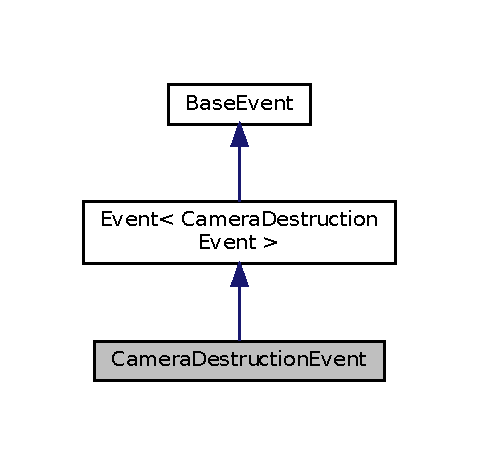
\includegraphics[width=230pt]{classCameraDestructionEvent__inherit__graph}
\end{center}
\end{figure}


Collaboration diagram for Camera\+Destruction\+Event\+:
\nopagebreak
\begin{figure}[H]
\begin{center}
\leavevmode
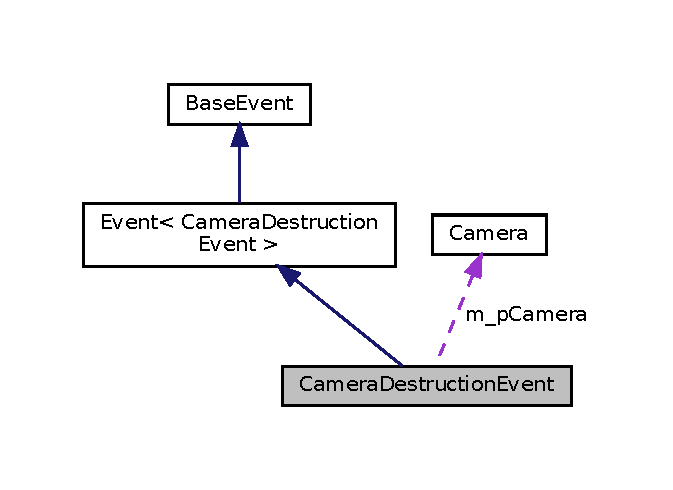
\includegraphics[width=323pt]{classCameraDestructionEvent__coll__graph}
\end{center}
\end{figure}
\subsection*{Public Member Functions}
\begin{DoxyCompactItemize}
\item 
\hyperlink{classCameraDestructionEvent_add18fdf0c985ffd437a0b204b51111c3}{Camera\+Destruction\+Event} (\hyperlink{classCamera}{Camera} $\ast$camera, size\+\_\+t id)
\begin{DoxyCompactList}\small\item\em Broadcasted when a camera gets destroyed. \end{DoxyCompactList}\item 
\mbox{\Hypertarget{classCameraDestructionEvent_a51b3e80cc36d6734c0758fb9b349b83e}\label{classCameraDestructionEvent_a51b3e80cc36d6734c0758fb9b349b83e}} 
virtual void \hyperlink{classCameraDestructionEvent_a51b3e80cc36d6734c0758fb9b349b83e}{operator()} () override
\begin{DoxyCompactList}\small\item\em Virtual function for mirror multicast invoke when event is invoked This is useful with some events for script delegate binds. \end{DoxyCompactList}\end{DoxyCompactItemize}
\subsection*{Public Attributes}
\begin{DoxyCompactItemize}
\item 
\mbox{\Hypertarget{classCameraDestructionEvent_a7051de5b07719f7730728ef27dce4df5}\label{classCameraDestructionEvent_a7051de5b07719f7730728ef27dce4df5}} 
\hyperlink{classCamera}{Camera} $\ast$ \hyperlink{classCameraDestructionEvent_a7051de5b07719f7730728ef27dce4df5}{m\+\_\+p\+Camera}
\begin{DoxyCompactList}\small\item\em \hyperlink{classCamera}{Camera} Pointer. \end{DoxyCompactList}\item 
\mbox{\Hypertarget{classCameraDestructionEvent_a227991598328cd699e22e8e33b9bbe72}\label{classCameraDestructionEvent_a227991598328cd699e22e8e33b9bbe72}} 
size\+\_\+t \hyperlink{classCameraDestructionEvent_a227991598328cd699e22e8e33b9bbe72}{m\+\_\+id}
\begin{DoxyCompactList}\small\item\em \hyperlink{classCamera}{Camera} ID. \end{DoxyCompactList}\end{DoxyCompactItemize}
\subsection*{Additional Inherited Members}


\subsection{Detailed Description}
Broadcasted when a camera gets destroyed. 

\subsection{Constructor \& Destructor Documentation}
\mbox{\Hypertarget{classCameraDestructionEvent_add18fdf0c985ffd437a0b204b51111c3}\label{classCameraDestructionEvent_add18fdf0c985ffd437a0b204b51111c3}} 
\index{Camera\+Destruction\+Event@{Camera\+Destruction\+Event}!Camera\+Destruction\+Event@{Camera\+Destruction\+Event}}
\index{Camera\+Destruction\+Event@{Camera\+Destruction\+Event}!Camera\+Destruction\+Event@{Camera\+Destruction\+Event}}
\subsubsection{\texorpdfstring{Camera\+Destruction\+Event()}{CameraDestructionEvent()}}
{\footnotesize\ttfamily Camera\+Destruction\+Event\+::\+Camera\+Destruction\+Event (\begin{DoxyParamCaption}\item[{\hyperlink{classCamera}{Camera} $\ast$}]{camera,  }\item[{size\+\_\+t}]{id }\end{DoxyParamCaption})\hspace{0.3cm}{\ttfamily [inline]}}



Broadcasted when a camera gets destroyed. 


\begin{DoxyParams}{Parameters}
{\em camera} & \\
\hline
{\em id} & \\
\hline
\end{DoxyParams}


The documentation for this class was generated from the following file\+:\begin{DoxyCompactItemize}
\item 
Events/\+Camera/\hyperlink{CameraEvents_8h}{Camera\+Events.\+h}\end{DoxyCompactItemize}

\hypertarget{structCameraInfo}{}\section{Camera\+Info Struct Reference}
\label{structCameraInfo}\index{Camera\+Info@{Camera\+Info}}


\hyperlink{classCamera}{Camera} Information.  




{\ttfamily \#include $<$Camera\+Manager.\+h$>$}



Collaboration diagram for Camera\+Info\+:
\nopagebreak
\begin{figure}[H]
\begin{center}
\leavevmode
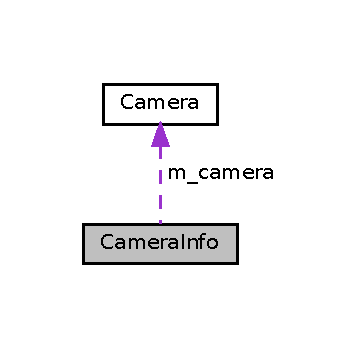
\includegraphics[width=172pt]{structCameraInfo__coll__graph}
\end{center}
\end{figure}
\subsection*{Public Member Functions}
\begin{DoxyCompactItemize}
\item 
\hyperlink{structCameraInfo_acaeb61d27869ecca978751caf05b4e22}{Camera\+Info} (\hyperlink{classCamera}{Camera} \&cam, size\+\_\+t x, size\+\_\+t y)
\begin{DoxyCompactList}\small\item\em Construct a new \hyperlink{classCamera}{Camera} Info object. \end{DoxyCompactList}\end{DoxyCompactItemize}
\subsection*{Public Attributes}
\begin{DoxyCompactItemize}
\item 
\mbox{\Hypertarget{structCameraInfo_a37cdbd4b4c81c6cfcb302651e16d253b}\label{structCameraInfo_a37cdbd4b4c81c6cfcb302651e16d253b}} 
\hyperlink{classCamera}{Camera} \& \hyperlink{structCameraInfo_a37cdbd4b4c81c6cfcb302651e16d253b}{m\+\_\+camera}
\begin{DoxyCompactList}\small\item\em \hyperlink{classCamera}{Camera} Object Reference. \end{DoxyCompactList}\item 
\mbox{\Hypertarget{structCameraInfo_ab3933b7d9bbbba4a5fe6d4a7b377a747}\label{structCameraInfo_ab3933b7d9bbbba4a5fe6d4a7b377a747}} 
size\+\_\+t \hyperlink{structCameraInfo_ab3933b7d9bbbba4a5fe6d4a7b377a747}{m\+\_\+left\+BottomX}
\begin{DoxyCompactList}\small\item\em Screen Left Bottom x-\/value. \end{DoxyCompactList}\item 
\mbox{\Hypertarget{structCameraInfo_a66ba9efc00aa351d35336e2971921f0e}\label{structCameraInfo_a66ba9efc00aa351d35336e2971921f0e}} 
size\+\_\+t \hyperlink{structCameraInfo_a66ba9efc00aa351d35336e2971921f0e}{m\+\_\+left\+BottomY}
\begin{DoxyCompactList}\small\item\em Screen Right Bottom y-\/value. \end{DoxyCompactList}\item 
\mbox{\Hypertarget{structCameraInfo_a7d129efd3cef38dfcffb37feacdbea41}\label{structCameraInfo_a7d129efd3cef38dfcffb37feacdbea41}} 
int \hyperlink{structCameraInfo_a7d129efd3cef38dfcffb37feacdbea41}{m\+\_\+z\+Order}
\begin{DoxyCompactList}\small\item\em Z order. \end{DoxyCompactList}\end{DoxyCompactItemize}


\subsection{Detailed Description}
\hyperlink{classCamera}{Camera} Information. 

\subsection{Constructor \& Destructor Documentation}
\mbox{\Hypertarget{structCameraInfo_acaeb61d27869ecca978751caf05b4e22}\label{structCameraInfo_acaeb61d27869ecca978751caf05b4e22}} 
\index{Camera\+Info@{Camera\+Info}!Camera\+Info@{Camera\+Info}}
\index{Camera\+Info@{Camera\+Info}!Camera\+Info@{Camera\+Info}}
\subsubsection{\texorpdfstring{Camera\+Info()}{CameraInfo()}}
{\footnotesize\ttfamily Camera\+Info\+::\+Camera\+Info (\begin{DoxyParamCaption}\item[{\hyperlink{classCamera}{Camera} \&}]{cam,  }\item[{size\+\_\+t}]{x,  }\item[{size\+\_\+t}]{y }\end{DoxyParamCaption})\hspace{0.3cm}{\ttfamily [inline]}}



Construct a new \hyperlink{classCamera}{Camera} Info object. 


\begin{DoxyParams}{Parameters}
{\em cam} & \\
\hline
{\em x} & \\
\hline
{\em y} & \\
\hline
\end{DoxyParams}


The documentation for this struct was generated from the following file\+:\begin{DoxyCompactItemize}
\item 
Managers/\hyperlink{CameraManager_8h}{Camera\+Manager.\+h}\end{DoxyCompactItemize}

\hypertarget{classCameraManager}{}\section{Camera\+Manager Class Reference}
\label{classCameraManager}\index{Camera\+Manager@{Camera\+Manager}}


Registers any created camera\textquotesingle{}s data This is important for any screen size or info change, the event must be passed to all cameras to update aspect ratios...  




{\ttfamily \#include $<$Camera\+Manager.\+h$>$}

\subsection*{Public Member Functions}
\begin{DoxyCompactItemize}
\item 
void \hyperlink{classCameraManager_a7667fa4d71bf8b1630c60d4e5e7864eb}{Update} (float dt)
\begin{DoxyCompactList}\small\item\em Not used. \end{DoxyCompactList}\item 
const \hyperlink{structCameraInfo}{Camera\+Info} \& \hyperlink{classCameraManager_ab4ec55062dac1028e8b781ec7bd94bf1}{Get\+Main\+Camera} () const
\begin{DoxyCompactList}\small\item\em Get the Main \hyperlink{classCamera}{Camera} object (index 0) \end{DoxyCompactList}\end{DoxyCompactItemize}


\subsection{Detailed Description}
Registers any created camera\textquotesingle{}s data This is important for any screen size or info change, the event must be passed to all cameras to update aspect ratios... 

\subsection{Member Function Documentation}
\mbox{\Hypertarget{classCameraManager_ab4ec55062dac1028e8b781ec7bd94bf1}\label{classCameraManager_ab4ec55062dac1028e8b781ec7bd94bf1}} 
\index{Camera\+Manager@{Camera\+Manager}!Get\+Main\+Camera@{Get\+Main\+Camera}}
\index{Get\+Main\+Camera@{Get\+Main\+Camera}!Camera\+Manager@{Camera\+Manager}}
\subsubsection{\texorpdfstring{Get\+Main\+Camera()}{GetMainCamera()}}
{\footnotesize\ttfamily const \hyperlink{structCameraInfo}{Camera\+Info} \& Camera\+Manager\+::\+Get\+Main\+Camera (\begin{DoxyParamCaption}{ }\end{DoxyParamCaption}) const}



Get the Main \hyperlink{classCamera}{Camera} object (index 0) 

\begin{DoxyReturn}{Returns}
const \hyperlink{structCameraInfo}{Camera\+Info}\& 
\end{DoxyReturn}
\mbox{\Hypertarget{classCameraManager_a7667fa4d71bf8b1630c60d4e5e7864eb}\label{classCameraManager_a7667fa4d71bf8b1630c60d4e5e7864eb}} 
\index{Camera\+Manager@{Camera\+Manager}!Update@{Update}}
\index{Update@{Update}!Camera\+Manager@{Camera\+Manager}}
\subsubsection{\texorpdfstring{Update()}{Update()}}
{\footnotesize\ttfamily void Camera\+Manager\+::\+Update (\begin{DoxyParamCaption}\item[{float}]{dt }\end{DoxyParamCaption})}



Not used. 


\begin{DoxyParams}{Parameters}
{\em dt} & \\
\hline
\end{DoxyParams}


The documentation for this class was generated from the following files\+:\begin{DoxyCompactItemize}
\item 
Managers/\hyperlink{CameraManager_8h}{Camera\+Manager.\+h}\item 
Managers/Camera\+Manager.\+cpp\end{DoxyCompactItemize}

\hypertarget{classCameraRegistrationEvent}{}\section{Camera\+Registration\+Event Class Reference}
\label{classCameraRegistrationEvent}\index{Camera\+Registration\+Event@{Camera\+Registration\+Event}}


Broadcasted when a camera gets created for registration.  




{\ttfamily \#include $<$Camera\+Events.\+h$>$}



Inheritance diagram for Camera\+Registration\+Event\+:
\nopagebreak
\begin{figure}[H]
\begin{center}
\leavevmode
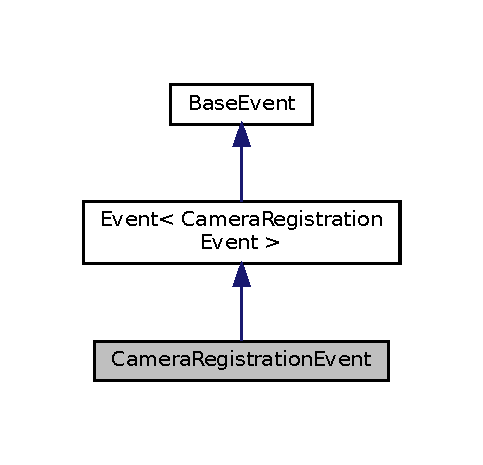
\includegraphics[width=232pt]{classCameraRegistrationEvent__inherit__graph}
\end{center}
\end{figure}


Collaboration diagram for Camera\+Registration\+Event\+:
\nopagebreak
\begin{figure}[H]
\begin{center}
\leavevmode
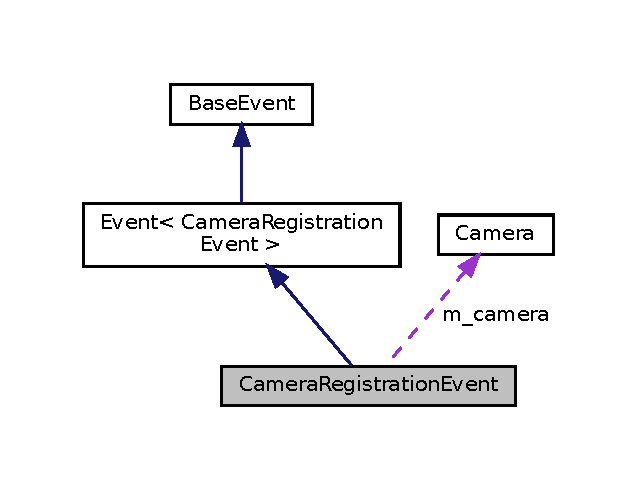
\includegraphics[width=306pt]{classCameraRegistrationEvent__coll__graph}
\end{center}
\end{figure}
\subsection*{Public Member Functions}
\begin{DoxyCompactItemize}
\item 
\hyperlink{classCameraRegistrationEvent_a9c432a3e04e803c4230592c9973be50a}{Camera\+Registration\+Event} (\hyperlink{classCamera}{Camera} \&r\+Camera, size\+\_\+t x\+Pos, size\+\_\+t y\+Pos)
\begin{DoxyCompactList}\small\item\em Broadcasted when a camera gets created for registration. \end{DoxyCompactList}\item 
\mbox{\Hypertarget{classCameraRegistrationEvent_a4134a5ad8c55691d0408e8259dfd2959}\label{classCameraRegistrationEvent_a4134a5ad8c55691d0408e8259dfd2959}} 
virtual void \hyperlink{classCameraRegistrationEvent_a4134a5ad8c55691d0408e8259dfd2959}{operator()} () override
\begin{DoxyCompactList}\small\item\em Virtual function for mirror multicast invoke when event is invoked This is useful with some events for script delegate binds. \end{DoxyCompactList}\end{DoxyCompactItemize}
\subsection*{Public Attributes}
\begin{DoxyCompactItemize}
\item 
\mbox{\Hypertarget{classCameraRegistrationEvent_ac49a8e11a215f7b21078e0fa6d496ad3}\label{classCameraRegistrationEvent_ac49a8e11a215f7b21078e0fa6d496ad3}} 
\hyperlink{classCamera}{Camera} \& \hyperlink{classCameraRegistrationEvent_ac49a8e11a215f7b21078e0fa6d496ad3}{m\+\_\+camera}
\begin{DoxyCompactList}\small\item\em \hyperlink{classCamera}{Camera} Reference. \end{DoxyCompactList}\item 
\mbox{\Hypertarget{classCameraRegistrationEvent_a903f23fc19015e14b309974c88783c14}\label{classCameraRegistrationEvent_a903f23fc19015e14b309974c88783c14}} 
size\+\_\+t \hyperlink{classCameraRegistrationEvent_a903f23fc19015e14b309974c88783c14}{m\+\_\+x\+View\+Port\+Pos}
\begin{DoxyCompactList}\small\item\em Position in Viewport x. \end{DoxyCompactList}\item 
\mbox{\Hypertarget{classCameraRegistrationEvent_a08e44509bad3f046e5ca458c309345d8}\label{classCameraRegistrationEvent_a08e44509bad3f046e5ca458c309345d8}} 
size\+\_\+t \hyperlink{classCameraRegistrationEvent_a08e44509bad3f046e5ca458c309345d8}{m\+\_\+y\+Viewport\+Pos}
\begin{DoxyCompactList}\small\item\em Position in Viewport y. \end{DoxyCompactList}\end{DoxyCompactItemize}
\subsection*{Additional Inherited Members}


\subsection{Detailed Description}
Broadcasted when a camera gets created for registration. 

\subsection{Constructor \& Destructor Documentation}
\mbox{\Hypertarget{classCameraRegistrationEvent_a9c432a3e04e803c4230592c9973be50a}\label{classCameraRegistrationEvent_a9c432a3e04e803c4230592c9973be50a}} 
\index{Camera\+Registration\+Event@{Camera\+Registration\+Event}!Camera\+Registration\+Event@{Camera\+Registration\+Event}}
\index{Camera\+Registration\+Event@{Camera\+Registration\+Event}!Camera\+Registration\+Event@{Camera\+Registration\+Event}}
\subsubsection{\texorpdfstring{Camera\+Registration\+Event()}{CameraRegistrationEvent()}}
{\footnotesize\ttfamily Camera\+Registration\+Event\+::\+Camera\+Registration\+Event (\begin{DoxyParamCaption}\item[{\hyperlink{classCamera}{Camera} \&}]{r\+Camera,  }\item[{size\+\_\+t}]{x\+Pos,  }\item[{size\+\_\+t}]{y\+Pos }\end{DoxyParamCaption})\hspace{0.3cm}{\ttfamily [inline]}}



Broadcasted when a camera gets created for registration. 


\begin{DoxyParams}{Parameters}
{\em r\+Camera} & \\
\hline
{\em x\+Pos} & \\
\hline
{\em y\+Pos} & \\
\hline
\end{DoxyParams}


The documentation for this class was generated from the following file\+:\begin{DoxyCompactItemize}
\item 
Events/\+Camera/\hyperlink{CameraEvents_8h}{Camera\+Events.\+h}\end{DoxyCompactItemize}

\hypertarget{classCameraSystem}{}\section{Camera\+System Class Reference}
\label{classCameraSystem}\index{Camera\+System@{Camera\+System}}


Inheritance diagram for Camera\+System\+:
\nopagebreak
\begin{figure}[H]
\begin{center}
\leavevmode
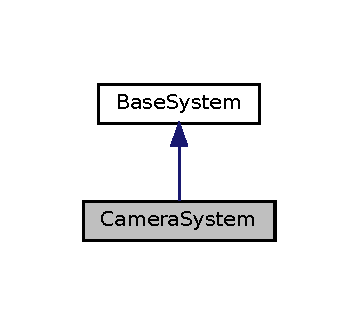
\includegraphics[width=172pt]{classCameraSystem__inherit__graph}
\end{center}
\end{figure}


Collaboration diagram for Camera\+System\+:
\nopagebreak
\begin{figure}[H]
\begin{center}
\leavevmode
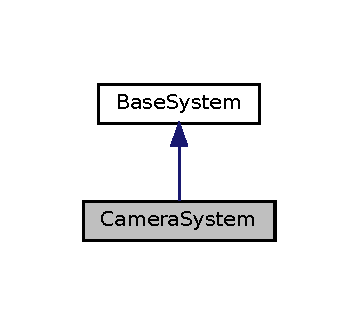
\includegraphics[width=172pt]{classCameraSystem__coll__graph}
\end{center}
\end{figure}
\subsection*{Public Member Functions}
\begin{DoxyCompactItemize}
\item 
virtual void \hyperlink{classCameraSystem_a2cbe7b251450e9693cf49759fba120e6}{Register\+\_\+\+Game\+Object} (\hyperlink{classGameObject}{Game\+Object} $\ast$go) override
\begin{DoxyCompactList}\small\item\em Registers \hyperlink{classGameObject}{Game\+Object} GO in this system. \end{DoxyCompactList}\item 
virtual void \hyperlink{classCameraSystem_ab0ea25c2a8f704f0a0674a3bc61ddd68}{Update} (float dt, \hyperlink{structBaseSystemCompNode}{Base\+System\+Comp\+Node} $\ast$comp\+Node) override
\begin{DoxyCompactList}\small\item\em Regular Update call. Called once per registered \hyperlink{classGameObject}{Game\+Object} by Update\+All\+Nodes. \end{DoxyCompactList}\end{DoxyCompactItemize}
\subsection*{Static Public Attributes}
\begin{DoxyCompactItemize}
\item 
\mbox{\Hypertarget{classCameraSystem_a321e590f18ebbd92290c3922d5c18924}\label{classCameraSystem_a321e590f18ebbd92290c3922d5c18924}} 
static unsigned int const {\bfseries static\+\_\+type} = \hyperlink{classBaseSystem_a7ef356edab3cfb02905e0a73a645b131}{Base\+System\+::number\+Of\+Types}++
\end{DoxyCompactItemize}
\subsection*{Additional Inherited Members}


\subsection{Member Function Documentation}
\mbox{\Hypertarget{classCameraSystem_a2cbe7b251450e9693cf49759fba120e6}\label{classCameraSystem_a2cbe7b251450e9693cf49759fba120e6}} 
\index{Camera\+System@{Camera\+System}!Register\+\_\+\+Game\+Object@{Register\+\_\+\+Game\+Object}}
\index{Register\+\_\+\+Game\+Object@{Register\+\_\+\+Game\+Object}!Camera\+System@{Camera\+System}}
\subsubsection{\texorpdfstring{Register\+\_\+\+Game\+Object()}{Register\_GameObject()}}
{\footnotesize\ttfamily void Camera\+System\+::\+Register\+\_\+\+Game\+Object (\begin{DoxyParamCaption}\item[{\hyperlink{classGameObject}{Game\+Object} $\ast$}]{go }\end{DoxyParamCaption})\hspace{0.3cm}{\ttfamily [override]}, {\ttfamily [virtual]}}



Registers \hyperlink{classGameObject}{Game\+Object} GO in this system. 


\begin{DoxyParams}{Parameters}
{\em go} & \\
\hline
\end{DoxyParams}


Implements \hyperlink{classBaseSystem}{Base\+System}.

\mbox{\Hypertarget{classCameraSystem_ab0ea25c2a8f704f0a0674a3bc61ddd68}\label{classCameraSystem_ab0ea25c2a8f704f0a0674a3bc61ddd68}} 
\index{Camera\+System@{Camera\+System}!Update@{Update}}
\index{Update@{Update}!Camera\+System@{Camera\+System}}
\subsubsection{\texorpdfstring{Update()}{Update()}}
{\footnotesize\ttfamily void Camera\+System\+::\+Update (\begin{DoxyParamCaption}\item[{float}]{dt,  }\item[{\hyperlink{structBaseSystemCompNode}{Base\+System\+Comp\+Node} $\ast$}]{comp\+Node }\end{DoxyParamCaption})\hspace{0.3cm}{\ttfamily [override]}, {\ttfamily [virtual]}}



Regular Update call. Called once per registered \hyperlink{classGameObject}{Game\+Object} by Update\+All\+Nodes. 


\begin{DoxyParams}{Parameters}
{\em dt} & \\
\hline
{\em comp\+Node} & \\
\hline
\end{DoxyParams}


Reimplemented from \hyperlink{classBaseSystem_a465191589a1ef8b8f3a8e20fa4656d47}{Base\+System}.



The documentation for this class was generated from the following files\+:\begin{DoxyCompactItemize}
\item 
Systems/Camera\+System.\+h\item 
Systems/Camera\+System.\+cpp\end{DoxyCompactItemize}

\hypertarget{structCameraUniformData}{}\section{Camera\+Uniform\+Data Struct Reference}
\label{structCameraUniformData}\index{Camera\+Uniform\+Data@{Camera\+Uniform\+Data}}
\subsection*{Public Attributes}
\begin{DoxyCompactItemize}
\item 
\mbox{\Hypertarget{structCameraUniformData_a01514edfff9acac810fd6a65a453840b}\label{structCameraUniformData_a01514edfff9acac810fd6a65a453840b}} 
float4x4 {\bfseries View\+Mat}
\item 
\mbox{\Hypertarget{structCameraUniformData_af55ae4b8ac680761b85b1204f5fcf22c}\label{structCameraUniformData_af55ae4b8ac680761b85b1204f5fcf22c}} 
float4x4 {\bfseries Inv\+View\+Mat}
\item 
\mbox{\Hypertarget{structCameraUniformData_a39bbf6ea3d4020f7e3c750ac3490a4d4}\label{structCameraUniformData_a39bbf6ea3d4020f7e3c750ac3490a4d4}} 
float4x4 {\bfseries Projection\+Mat}
\item 
\mbox{\Hypertarget{structCameraUniformData_a44393ccde4c334f6b38dc571c3f80a27}\label{structCameraUniformData_a44393ccde4c334f6b38dc571c3f80a27}} 
float4x4 {\bfseries Inv\+Projection\+Mat}
\item 
\mbox{\Hypertarget{structCameraUniformData_a504182d0502dff132871c8bf137c6210}\label{structCameraUniformData_a504182d0502dff132871c8bf137c6210}} 
float4x4 {\bfseries View\+Projection\+Mat}
\item 
\mbox{\Hypertarget{structCameraUniformData_acbf3d5b25e11cbc2383d65681dd52e19}\label{structCameraUniformData_acbf3d5b25e11cbc2383d65681dd52e19}} 
float4x4 {\bfseries Inv\+View\+Projection\+Mat}
\item 
\mbox{\Hypertarget{structCameraUniformData_a02e98ef42f0ec1453402e24d71950c7f}\label{structCameraUniformData_a02e98ef42f0ec1453402e24d71950c7f}} 
float4 {\bfseries Camera\+Position}
\item 
\mbox{\Hypertarget{structCameraUniformData_ace24d69a7608996740a32a51a3bb3226}\label{structCameraUniformData_ace24d69a7608996740a32a51a3bb3226}} 
float2 {\bfseries Camera\+Viewport\+Size}
\end{DoxyCompactItemize}


The documentation for this struct was generated from the following file\+:\begin{DoxyCompactItemize}
\item 
Shaders/Shading.\+h\end{DoxyCompactItemize}

\hypertarget{classCastResult}{}\section{Cast\+Result Class Reference}
\label{classCastResult}\index{Cast\+Result@{Cast\+Result}}
\subsection*{Public Member Functions}
\begin{DoxyCompactItemize}
\item 
\mbox{\Hypertarget{classCastResult_a0bfa7f1f5b34b2a2c6846ab07e10584c}\label{classCastResult_a0bfa7f1f5b34b2a2c6846ab07e10584c}} 
{\bfseries Cast\+Result} (void $\ast$client\+Data)
\item 
\mbox{\Hypertarget{classCastResult_aac9e9fc20559d0312a4a2b67472e21ad}\label{classCastResult_aac9e9fc20559d0312a4a2b67472e21ad}} 
{\bfseries Cast\+Result} (void $\ast$client\+Data, float time)
\item 
\mbox{\Hypertarget{classCastResult_aa93d9222beba3f31dafeba8761ab0979}\label{classCastResult_aa93d9222beba3f31dafeba8761ab0979}} 
bool {\bfseries operator$<$} (const \hyperlink{classCastResult}{Cast\+Result} \&rhs) const
\end{DoxyCompactItemize}
\subsection*{Public Attributes}
\begin{DoxyCompactItemize}
\item 
\mbox{\Hypertarget{classCastResult_a8bdd91efbc7ac7c3cee5692bb1cd12ff}\label{classCastResult_a8bdd91efbc7ac7c3cee5692bb1cd12ff}} 
float {\bfseries m\+\_\+\+Time}
\item 
\mbox{\Hypertarget{classCastResult_a05176a3b71d4958ba65e99c800ecadb3}\label{classCastResult_a05176a3b71d4958ba65e99c800ecadb3}} 
void $\ast$ {\bfseries m\+\_\+\+Client\+Data}
\end{DoxyCompactItemize}


The documentation for this class was generated from the following files\+:\begin{DoxyCompactItemize}
\item 
Physics/\+Spatial\+Partition/Cast\+Results.\+h\item 
Physics/\+Spatial\+Partition/Cast\+Results.\+cpp\end{DoxyCompactItemize}

\hypertarget{classCastResults}{}\section{Cast\+Results Class Reference}
\label{classCastResults}\index{Cast\+Results@{Cast\+Results}}
\subsection*{Public Types}
\begin{DoxyCompactItemize}
\item 
\mbox{\Hypertarget{classCastResults_a96c98918bc6f75030603ae54a470632a}\label{classCastResults_a96c98918bc6f75030603ae54a470632a}} 
typedef std\+::vector$<$ \hyperlink{classCastResult}{Cast\+Result} $>$ {\bfseries Results}
\end{DoxyCompactItemize}
\subsection*{Public Member Functions}
\begin{DoxyCompactItemize}
\item 
\mbox{\Hypertarget{classCastResults_a62ee1ac3a8107eb7f8be4d991e9c47c5}\label{classCastResults_a62ee1ac3a8107eb7f8be4d991e9c47c5}} 
void {\bfseries Add\+Result} (const \hyperlink{classCastResult}{Cast\+Result} \&result)
\end{DoxyCompactItemize}
\subsection*{Public Attributes}
\begin{DoxyCompactItemize}
\item 
\mbox{\Hypertarget{classCastResults_acb2777d80f4f46a8fc1954ea9fd7b431}\label{classCastResults_acb2777d80f4f46a8fc1954ea9fd7b431}} 
Results {\bfseries m\+\_\+\+Results}
\end{DoxyCompactItemize}


The documentation for this class was generated from the following files\+:\begin{DoxyCompactItemize}
\item 
Physics/\+Spatial\+Partition/Cast\+Results.\+h\item 
Physics/\+Spatial\+Partition/Cast\+Results.\+cpp\end{DoxyCompactItemize}

\hypertarget{structClearValue}{}\section{Clear\+Value Struct Reference}
\label{structClearValue}\index{Clear\+Value@{Clear\+Value}}
\subsection*{Public Attributes}
\begin{DoxyCompactItemize}
\item 
\mbox{\Hypertarget{structClearValue_aa59a944b6e8b81bed2fc7c7948d5f1a6}\label{structClearValue_aa59a944b6e8b81bed2fc7c7948d5f1a6}} 
\begin{tabbing}
xx\=xx\=xx\=xx\=xx\=xx\=xx\=xx\=xx\=\kill
union \{\\
\mbox{\Hypertarget{unionClearValue_1_1_0D8_a5b4b7eb2d748b46e2fba13a00ee48551}\label{unionClearValue_1_1_0D8_a5b4b7eb2d748b46e2fba13a00ee48551}} 
\>struct \{\\
\>\>float {\bfseries r}\\
\>\>float {\bfseries g}\\
\>\>float {\bfseries b}\\
\>\>float {\bfseries a}\\
\>\} \\
\mbox{\Hypertarget{unionClearValue_1_1_0D8_ad4b76c6f6ccb1842ed29c79046dbe977}\label{unionClearValue_1_1_0D8_ad4b76c6f6ccb1842ed29c79046dbe977}} 
\>struct \{\\
\>\>float {\bfseries m\_depth}\\
\>\>uint32\_t {\bfseries m\_stencil}\\
\>\} \\
\}; \\

\end{tabbing}\end{DoxyCompactItemize}


The documentation for this struct was generated from the following file\+:\begin{DoxyCompactItemize}
\item 
Graphics/Texture.\+h\end{DoxyCompactItemize}

\hypertarget{structClipInfo}{}\section{Clip\+Info Struct Reference}
\label{structClipInfo}\index{Clip\+Info@{Clip\+Info}}
\subsection*{Public Member Functions}
\begin{DoxyCompactItemize}
\item 
\mbox{\Hypertarget{structClipInfo_a81cb0f8c29b822520bc9d3b6aaaf31de}\label{structClipInfo_a81cb0f8c29b822520bc9d3b6aaaf31de}} 
{\bfseries R\+T\+T\+R\+\_\+\+E\+N\+A\+B\+LE} ()
\end{DoxyCompactItemize}
\subsection*{Public Attributes}
\begin{DoxyCompactItemize}
\item 
\mbox{\Hypertarget{structClipInfo_afd5ffbc541b7d16140e3363c689b4c49}\label{structClipInfo_afd5ffbc541b7d16140e3363c689b4c49}} 
std\+::string {\bfseries name}
\item 
\mbox{\Hypertarget{structClipInfo_a1552b48f64dcbc1e31dbb63e4db8366a}\label{structClipInfo_a1552b48f64dcbc1e31dbb63e4db8366a}} 
std\+::string {\bfseries path}
\item 
\mbox{\Hypertarget{structClipInfo_aeacd9bb55941fe62d2da4802510856ae}\label{structClipInfo_aeacd9bb55941fe62d2da4802510856ae}} 
bool {\bfseries loops}
\item 
\mbox{\Hypertarget{structClipInfo_aee66f2e0a2e4c01f0ede2b3ac7b65b26}\label{structClipInfo_aee66f2e0a2e4c01f0ede2b3ac7b65b26}} 
{\bfseries R\+T\+T\+R\+\_\+\+R\+E\+G\+I\+S\+T\+R\+A\+T\+I\+O\+N\+\_\+\+F\+R\+I\+E\+ND}
\end{DoxyCompactItemize}


The documentation for this struct was generated from the following files\+:\begin{DoxyCompactItemize}
\item 
Components/Animation\+Component.\+h\item 
Components/Animation\+Component.\+cpp\end{DoxyCompactItemize}

\hypertarget{classCollisionManifold}{}\section{Collision\+Manifold Class Reference}
\label{classCollisionManifold}\index{Collision\+Manifold@{Collision\+Manifold}}


Collaboration diagram for Collision\+Manifold\+:
\nopagebreak
\begin{figure}[H]
\begin{center}
\leavevmode
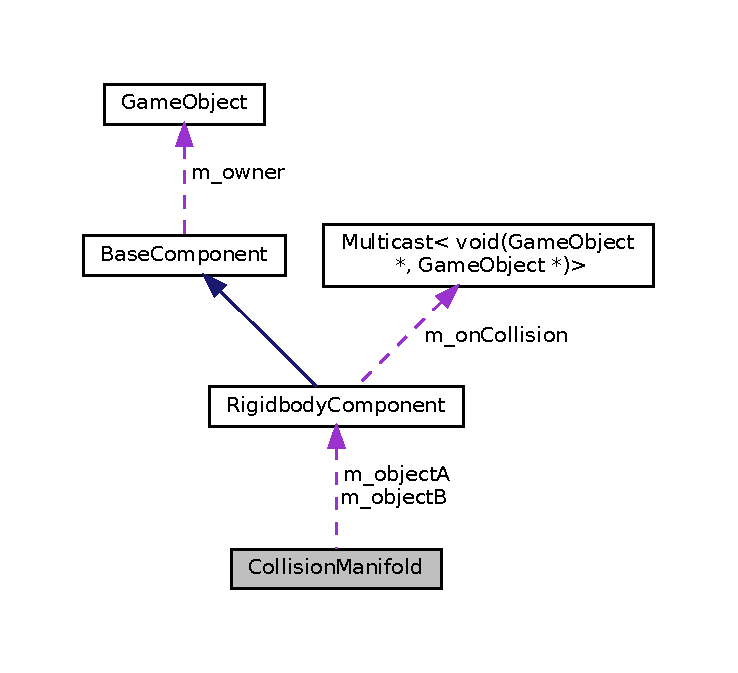
\includegraphics[width=350pt]{classCollisionManifold__coll__graph}
\end{center}
\end{figure}
\subsection*{Public Member Functions}
\begin{DoxyCompactItemize}
\item 
\mbox{\Hypertarget{classCollisionManifold_a46e84805aa00f1773719d79f2308deae}\label{classCollisionManifold_a46e84805aa00f1773719d79f2308deae}} 
{\bfseries Collision\+Manifold} (const \hyperlink{classCollisionManifold}{Collision\+Manifold} \&rhs)
\item 
\mbox{\Hypertarget{classCollisionManifold_aa037e82ecbe29d22f28427eeef01676b}\label{classCollisionManifold_aa037e82ecbe29d22f28427eeef01676b}} 
\hyperlink{classCollisionManifold}{Collision\+Manifold} \& {\bfseries operator=} (const \hyperlink{classCollisionManifold}{Collision\+Manifold} \&rhs)
\end{DoxyCompactItemize}
\subsection*{Public Attributes}
\begin{DoxyCompactItemize}
\item 
\mbox{\Hypertarget{classCollisionManifold_acc19a876530a865b75ed5c347aed8e16}\label{classCollisionManifold_acc19a876530a865b75ed5c347aed8e16}} 
\hyperlink{classRigidbodyComponent}{Rigidbody\+Component} $\ast$ {\bfseries m\+\_\+objectA}
\item 
\mbox{\Hypertarget{classCollisionManifold_a9687be8c297bde4d747befda177afbb6}\label{classCollisionManifold_a9687be8c297bde4d747befda177afbb6}} 
\hyperlink{classRigidbodyComponent}{Rigidbody\+Component} $\ast$ {\bfseries m\+\_\+objectB}
\item 
\mbox{\Hypertarget{classCollisionManifold_aa6bee4bd56bf5cf54993eb68ae8e8a80}\label{classCollisionManifold_aa6bee4bd56bf5cf54993eb68ae8e8a80}} 
Vector3 {\bfseries m\+\_\+pA}
\item 
\mbox{\Hypertarget{classCollisionManifold_a99023627d612e6adf5d250332e8a5ea4}\label{classCollisionManifold_a99023627d612e6adf5d250332e8a5ea4}} 
Vector3 {\bfseries m\+\_\+pB}
\item 
\mbox{\Hypertarget{classCollisionManifold_a0e49d92c5442e191fc72081c4000657e}\label{classCollisionManifold_a0e49d92c5442e191fc72081c4000657e}} 
Vector3 {\bfseries m\+\_\+normal}
\item 
\mbox{\Hypertarget{classCollisionManifold_a147ed5dd2971186308764d5faa640219}\label{classCollisionManifold_a147ed5dd2971186308764d5faa640219}} 
float {\bfseries m\+\_\+depth}
\item 
\mbox{\Hypertarget{classCollisionManifold_af352403a375481087f37f0e3a463d82f}\label{classCollisionManifold_af352403a375481087f37f0e3a463d82f}} 
bool {\bfseries m\+\_\+is\+Colliding}
\end{DoxyCompactItemize}


The documentation for this class was generated from the following files\+:\begin{DoxyCompactItemize}
\item 
Physics/\+Gjk/\hyperlink{CollisionManifold_8h}{Collision\+Manifold.\+h}\item 
Physics/\+Gjk/\hyperlink{CollisionManifold_8cpp}{Collision\+Manifold.\+cpp}\end{DoxyCompactItemize}

\hypertarget{classCollisionTable}{}\section{Collision\+Table Class Reference}
\label{classCollisionTable}\index{Collision\+Table@{Collision\+Table}}
\subsection*{Public Types}
\begin{DoxyCompactItemize}
\item 
\mbox{\Hypertarget{classCollisionTable_abec7701fa63dce6d59a0804b0ba1a69e}\label{classCollisionTable_abec7701fa63dce6d59a0804b0ba1a69e}} 
enum {\bfseries Collision\+Mask} \{ {\bfseries N\+UM}
 \}
\end{DoxyCompactItemize}
\subsection*{Public Member Functions}
\begin{DoxyCompactItemize}
\item 
\mbox{\Hypertarget{classCollisionTable_a1b9fda1f06ee74f2ac2539b8676322e4}\label{classCollisionTable_a1b9fda1f06ee74f2ac2539b8676322e4}} 
void {\bfseries Init\+Collision\+Matrix} ()
\item 
\mbox{\Hypertarget{classCollisionTable_a21c09fb6803e3da3deb9ea9b12648f27}\label{classCollisionTable_a21c09fb6803e3da3deb9ea9b12648f27}} 
bool {\bfseries Check\+Collision\+Matrix} (Collision\+Mask obj1, Collision\+Mask obj2) const
\end{DoxyCompactItemize}


The documentation for this class was generated from the following files\+:\begin{DoxyCompactItemize}
\item 
Physics/Collision\+Table.\+h\item 
Physics/Collision\+Table.\+cpp\end{DoxyCompactItemize}

\hypertarget{classDX_1_1com__exception}{}\section{DX\+:\+:com\+\_\+exception Class Reference}
\label{classDX_1_1com__exception}\index{D\+X\+::com\+\_\+exception@{D\+X\+::com\+\_\+exception}}


Inheritance diagram for DX\+:\+:com\+\_\+exception\+:\nopagebreak
\begin{figure}[H]
\begin{center}
\leavevmode
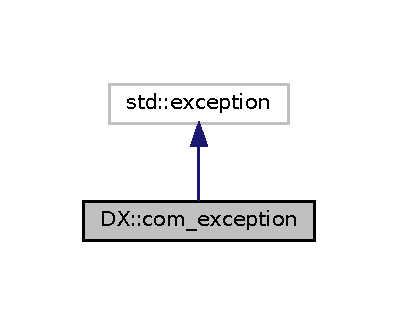
\includegraphics[width=191pt]{classDX_1_1com__exception__inherit__graph}
\end{center}
\end{figure}


Collaboration diagram for DX\+:\+:com\+\_\+exception\+:\nopagebreak
\begin{figure}[H]
\begin{center}
\leavevmode
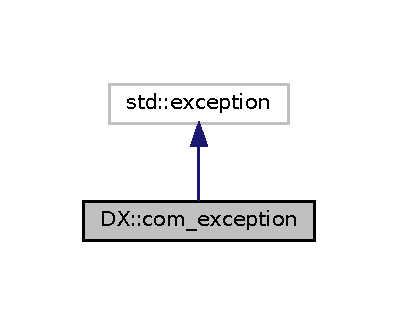
\includegraphics[width=191pt]{classDX_1_1com__exception__coll__graph}
\end{center}
\end{figure}
\subsection*{Public Member Functions}
\begin{DoxyCompactItemize}
\item 
\mbox{\Hypertarget{classDX_1_1com__exception_aa1867f0d21fb5d5cdac40d79cfa07ffb}\label{classDX_1_1com__exception_aa1867f0d21fb5d5cdac40d79cfa07ffb}} 
{\bfseries com\+\_\+exception} (H\+R\+E\+S\+U\+LT hr)
\item 
\mbox{\Hypertarget{classDX_1_1com__exception_aec8c85514b6908b1ddc794d7ed18e9e5}\label{classDX_1_1com__exception_aec8c85514b6908b1ddc794d7ed18e9e5}} 
virtual const char $\ast$ {\bfseries what} () const override
\end{DoxyCompactItemize}


The documentation for this class was generated from the following file\+:\begin{DoxyCompactItemize}
\item 
Graphics/d3d\+Utils.\+h\end{DoxyCompactItemize}

\hypertarget{structComputePipelineDesc}{}\section{Compute\+Pipeline\+Desc Struct Reference}
\label{structComputePipelineDesc}\index{Compute\+Pipeline\+Desc@{Compute\+Pipeline\+Desc}}


Collaboration diagram for Compute\+Pipeline\+Desc\+:\nopagebreak
\begin{figure}[H]
\begin{center}
\leavevmode
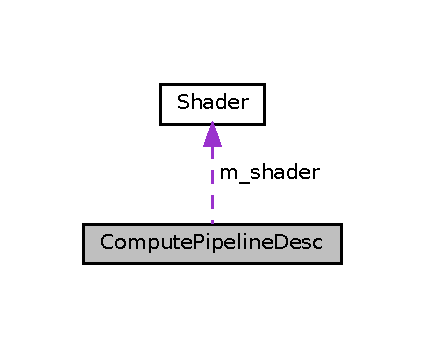
\includegraphics[width=204pt]{structComputePipelineDesc__coll__graph}
\end{center}
\end{figure}
\subsection*{Public Attributes}
\begin{DoxyCompactItemize}
\item 
\mbox{\Hypertarget{structComputePipelineDesc_a54a7e5b14a70eb58b96ed98246f7d123}\label{structComputePipelineDesc_a54a7e5b14a70eb58b96ed98246f7d123}} 
\hyperlink{classShader}{Shader} $\ast$ {\bfseries m\+\_\+shader}
\end{DoxyCompactItemize}


The documentation for this struct was generated from the following file\+:\begin{DoxyCompactItemize}
\item 
Graphics/Pipeline.\+h\end{DoxyCompactItemize}

\hypertarget{structConstantHaloEffectData}{}\section{Constant\+Halo\+Effect\+Data Struct Reference}
\label{structConstantHaloEffectData}\index{Constant\+Halo\+Effect\+Data@{Constant\+Halo\+Effect\+Data}}
\subsection*{Public Attributes}
\begin{DoxyCompactItemize}
\item 
\mbox{\Hypertarget{structConstantHaloEffectData_a54b15ba145326eeb73aff33405f9ad15}\label{structConstantHaloEffectData_a54b15ba145326eeb73aff33405f9ad15}} 
float4 {\bfseries Halo\+Position}
\item 
\mbox{\Hypertarget{structConstantHaloEffectData_aa8681074688bc02daf1ffa1e6c5ccfb1}\label{structConstantHaloEffectData_aa8681074688bc02daf1ffa1e6c5ccfb1}} 
float4 {\bfseries Halo\+Color}
\item 
\mbox{\Hypertarget{structConstantHaloEffectData_a3923463615dc35df5f3ab39f32da70e7}\label{structConstantHaloEffectData_a3923463615dc35df5f3ab39f32da70e7}} 
float4 {\bfseries Halo\+Misc\+Data}
\item 
\mbox{\Hypertarget{structConstantHaloEffectData_ad21e611ff6b297ca7391477e3148ec5d}\label{structConstantHaloEffectData_ad21e611ff6b297ca7391477e3148ec5d}} 
float4 {\bfseries Halo\+Misc\+Data2}
\end{DoxyCompactItemize}


The documentation for this struct was generated from the following file\+:\begin{DoxyCompactItemize}
\item 
Shaders/Shading.\+h\end{DoxyCompactItemize}

\hypertarget{structConstantPointLightData}{}\section{Constant\+Point\+Light\+Data Struct Reference}
\label{structConstantPointLightData}\index{Constant\+Point\+Light\+Data@{Constant\+Point\+Light\+Data}}
\subsection*{Public Attributes}
\begin{DoxyCompactItemize}
\item 
\mbox{\Hypertarget{structConstantPointLightData_ade4754202337060d29034a8273a58195}\label{structConstantPointLightData_ade4754202337060d29034a8273a58195}} 
float4 {\bfseries Light\+Position}
\item 
\mbox{\Hypertarget{structConstantPointLightData_a2582f88b45d7430cde1f3578f67a1200}\label{structConstantPointLightData_a2582f88b45d7430cde1f3578f67a1200}} 
float4 {\bfseries Light\+Color}
\item 
\mbox{\Hypertarget{structConstantPointLightData_adfcad818cf7c1c0a4c17b5e17ec2ca4d}\label{structConstantPointLightData_adfcad818cf7c1c0a4c17b5e17ec2ca4d}} 
float4 {\bfseries Light\+Misc\+Data}
\end{DoxyCompactItemize}


The documentation for this struct was generated from the following file\+:\begin{DoxyCompactItemize}
\item 
Shaders/Shading.\+h\end{DoxyCompactItemize}

\hypertarget{classConstraint}{}\section{Constraint Class Reference}
\label{classConstraint}\index{Constraint@{Constraint}}


Collaboration diagram for Constraint\+:\nopagebreak
\begin{figure}[H]
\begin{center}
\leavevmode
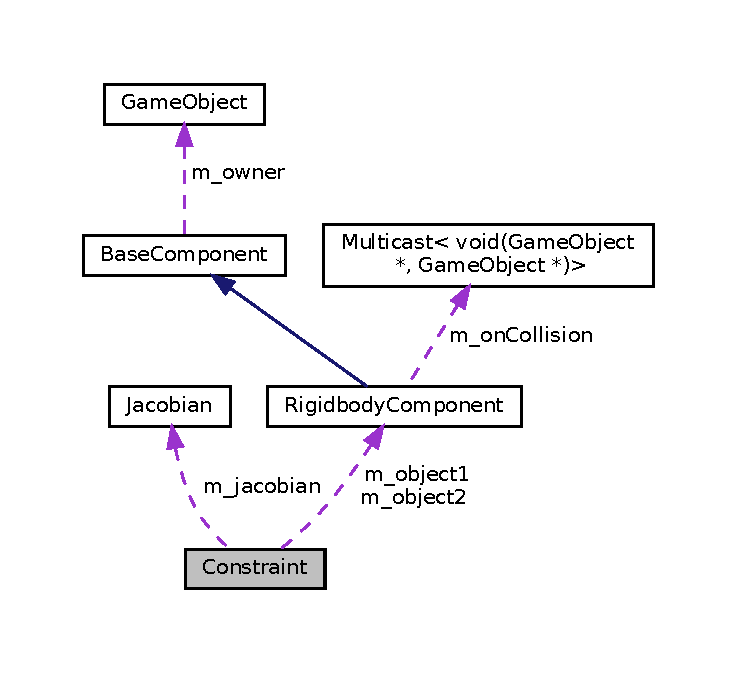
\includegraphics[width=350pt]{classConstraint__coll__graph}
\end{center}
\end{figure}
\subsection*{Public Member Functions}
\begin{DoxyCompactItemize}
\item 
\mbox{\Hypertarget{classConstraint_a395b6ff4b983af67254c5dfe9fdf6bb9}\label{classConstraint_a395b6ff4b983af67254c5dfe9fdf6bb9}} 
{\bfseries Constraint} (\hyperlink{classRigidbodyComponent}{Rigidbody\+Component} $\ast$obj1, \hyperlink{classRigidbodyComponent}{Rigidbody\+Component} $\ast$obj2, float depth=0.\+0f)
\item 
\mbox{\Hypertarget{classConstraint_a4b19008d8d9a6965bfc90111e5cc4efd}\label{classConstraint_a4b19008d8d9a6965bfc90111e5cc4efd}} 
void {\bfseries Calculate\+Normal\+Jacobian} (const Vector3 \&normal, const Vector3 \&pointA, const Vector3 \&pointB)
\end{DoxyCompactItemize}
\subsection*{Static Public Member Functions}
\begin{DoxyCompactItemize}
\item 
\mbox{\Hypertarget{classConstraint_ad59276ed90da13e5169f411a0b51329d}\label{classConstraint_ad59276ed90da13e5169f411a0b51329d}} 
static void {\bfseries Calculate\+Friction\+Jacobians} (const Vector3 \&normal, const Vector3 \&pointA, const Vector3 \&pointB, \hyperlink{classConstraint}{Constraint} \&constraint\+Friction1, \hyperlink{classConstraint}{Constraint} \&constraint\+Friction2)
\item 
\mbox{\Hypertarget{classConstraint_ae458b57a23e5c4f49654ac8fbb37b3e8}\label{classConstraint_ae458b57a23e5c4f49654ac8fbb37b3e8}} 
static void {\bfseries To\+Matrix4} (Matrix \&result, const \hyperlink{classJacobian}{Jacobian} \&jacobian)
\end{DoxyCompactItemize}
\subsection*{Public Attributes}
\begin{DoxyCompactItemize}
\item 
\mbox{\Hypertarget{classConstraint_a81be9de1b027d83afc88075cac8b5b4b}\label{classConstraint_a81be9de1b027d83afc88075cac8b5b4b}} 
\hyperlink{classJacobian}{Jacobian} {\bfseries m\+\_\+jacobian}
\item 
\mbox{\Hypertarget{classConstraint_a9bbea2866cb6f593f7be5422357ef43f}\label{classConstraint_a9bbea2866cb6f593f7be5422357ef43f}} 
\hyperlink{classRigidbodyComponent}{Rigidbody\+Component} $\ast$ {\bfseries m\+\_\+object1}
\item 
\mbox{\Hypertarget{classConstraint_a927b633621d426d3d049fe9e44b8bae1}\label{classConstraint_a927b633621d426d3d049fe9e44b8bae1}} 
\hyperlink{classRigidbodyComponent}{Rigidbody\+Component} $\ast$ {\bfseries m\+\_\+object2}
\item 
\mbox{\Hypertarget{classConstraint_aaabf19e98bae7a66b87d8a726316b20a}\label{classConstraint_aaabf19e98bae7a66b87d8a726316b20a}} 
Vector3 {\bfseries m\+\_\+normal}
\item 
\mbox{\Hypertarget{classConstraint_a4f7dae1972c717b15fa22a255bcb12f6}\label{classConstraint_a4f7dae1972c717b15fa22a255bcb12f6}} 
float {\bfseries m\+\_\+bias}
\item 
\mbox{\Hypertarget{classConstraint_a4e856baff516350a810ea3bf0a840450}\label{classConstraint_a4e856baff516350a810ea3bf0a840450}} 
float {\bfseries m\+\_\+lambda}
\item 
\mbox{\Hypertarget{classConstraint_ac3fdb5d9607837f03830b1874649a1cf}\label{classConstraint_ac3fdb5d9607837f03830b1874649a1cf}} 
float {\bfseries m\+\_\+depth\+Pen}
\end{DoxyCompactItemize}


The documentation for this class was generated from the following files\+:\begin{DoxyCompactItemize}
\item 
Physics/Constraint.\+h\item 
Physics/Constraint.\+cpp\end{DoxyCompactItemize}

\hypertarget{classContact}{}\section{Contact Class Reference}
\label{classContact}\index{Contact@{Contact}}


Stores all the information relative to the contact.  




{\ttfamily \#include $<$Constraint.\+h$>$}



Collaboration diagram for Contact\+:
\nopagebreak
\begin{figure}[H]
\begin{center}
\leavevmode
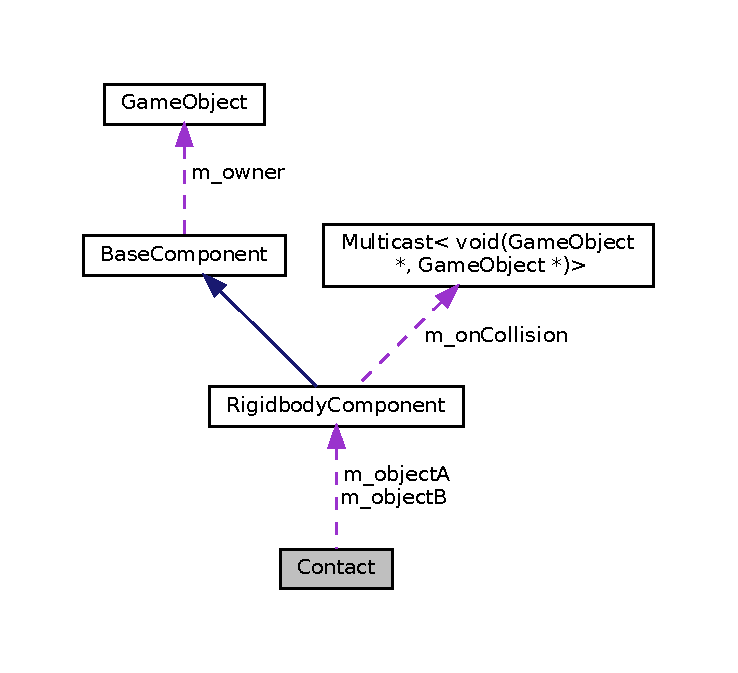
\includegraphics[width=350pt]{classContact__coll__graph}
\end{center}
\end{figure}
\subsection*{Public Member Functions}
\begin{DoxyCompactItemize}
\item 
\mbox{\Hypertarget{classContact_a1af30adc27b3cc1b971dcfe01959f9e9}\label{classContact_a1af30adc27b3cc1b971dcfe01959f9e9}} 
void \hyperlink{classContact_a1af30adc27b3cc1b971dcfe01959f9e9}{Build\+Constraints} ()
\begin{DoxyCompactList}\small\item\em Builds the 3 constraints for the contact from the previously initialized data. \end{DoxyCompactList}\end{DoxyCompactItemize}
\subsection*{Public Attributes}
\begin{DoxyCompactItemize}
\item 
\mbox{\Hypertarget{classContact_a5db355d00ddb18ce037309fb6cbc9500}\label{classContact_a5db355d00ddb18ce037309fb6cbc9500}} 
std\+::vector$<$ \hyperlink{classConstraint}{Constraint} $>$ {\bfseries m\+\_\+constraints}
\item 
\mbox{\Hypertarget{classContact_a9380549ad60a64820bb6ed0a3caf4e97}\label{classContact_a9380549ad60a64820bb6ed0a3caf4e97}} 
\hyperlink{classRigidbodyComponent}{Rigidbody\+Component} $\ast$ {\bfseries m\+\_\+objectA}
\item 
\mbox{\Hypertarget{classContact_a9f1e0f5aa29a630f107040c33961066a}\label{classContact_a9f1e0f5aa29a630f107040c33961066a}} 
\hyperlink{classRigidbodyComponent}{Rigidbody\+Component} $\ast$ {\bfseries m\+\_\+objectB}
\item 
\mbox{\Hypertarget{classContact_a6d0ef9e980ba29be6929f5aa62047f17}\label{classContact_a6d0ef9e980ba29be6929f5aa62047f17}} 
Vector3 {\bfseries m\+\_\+p\+A\+Local}
\item 
\mbox{\Hypertarget{classContact_a9d86be919bd954292afec22b844a2800}\label{classContact_a9d86be919bd954292afec22b844a2800}} 
Vector3 {\bfseries m\+\_\+p\+B\+Local}
\item 
\mbox{\Hypertarget{classContact_a50c33e277ddeb3bd1f6ab69ee91e00e7}\label{classContact_a50c33e277ddeb3bd1f6ab69ee91e00e7}} 
Vector3 {\bfseries m\+\_\+pA}
\item 
\mbox{\Hypertarget{classContact_a29ab504566025807593cc61f9348695a}\label{classContact_a29ab504566025807593cc61f9348695a}} 
Vector3 {\bfseries m\+\_\+pB}
\item 
\mbox{\Hypertarget{classContact_a351480a3ed43b421ee758c3c8ec33e2c}\label{classContact_a351480a3ed43b421ee758c3c8ec33e2c}} 
float {\bfseries m\+\_\+depth}
\item 
\mbox{\Hypertarget{classContact_af92b4be8a55d8655e0e3264d5f83f40c}\label{classContact_af92b4be8a55d8655e0e3264d5f83f40c}} 
Vector3 {\bfseries m\+\_\+normal}
\end{DoxyCompactItemize}


\subsection{Detailed Description}
Stores all the information relative to the contact. 

The documentation for this class was generated from the following files\+:\begin{DoxyCompactItemize}
\item 
Physics/\hyperlink{Constraint_8h}{Constraint.\+h}\item 
Physics/\hyperlink{Constraint_8cpp}{Constraint.\+cpp}\end{DoxyCompactItemize}

\hypertarget{classContactManifold}{}\section{Contact\+Manifold Class Reference}
\label{classContactManifold}\index{Contact\+Manifold@{Contact\+Manifold}}


Collaboration diagram for Contact\+Manifold\+:\nopagebreak
\begin{figure}[H]
\begin{center}
\leavevmode
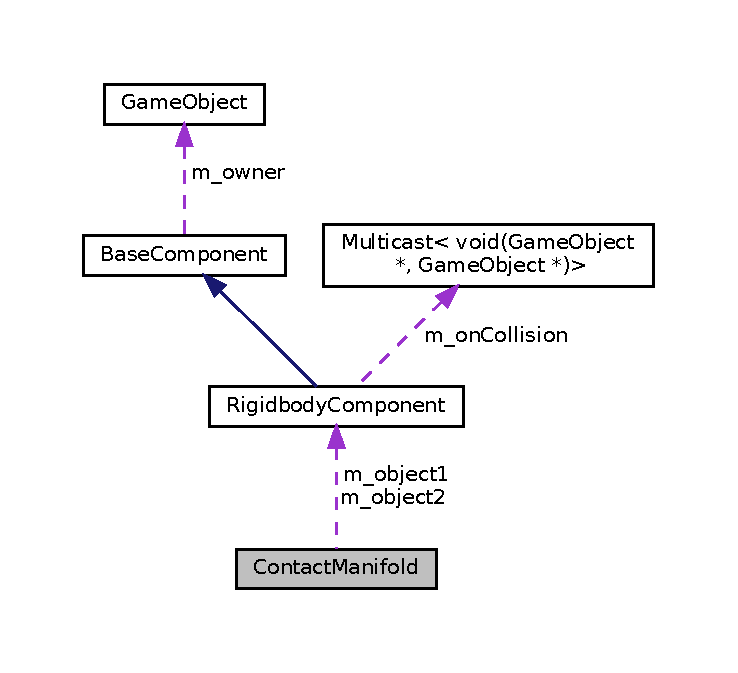
\includegraphics[width=350pt]{classContactManifold__coll__graph}
\end{center}
\end{figure}
\subsection*{Public Member Functions}
\begin{DoxyCompactItemize}
\item 
\mbox{\Hypertarget{classContactManifold_a5f97e21f2f679383c0484fb03064d4ac}\label{classContactManifold_a5f97e21f2f679383c0484fb03064d4ac}} 
{\bfseries Contact\+Manifold} (\hyperlink{classContact}{Contact} \&collision)
\item 
\mbox{\Hypertarget{classContactManifold_ab435616e119010a5904ff0833519bf52}\label{classContactManifold_ab435616e119010a5904ff0833519bf52}} 
void {\bfseries Proccess\+Collision} (\hyperlink{classContact}{Contact} \&collision)
\item 
\mbox{\Hypertarget{classContactManifold_a6fdcb82f3b35f2d9e7f5d6710a6c3119}\label{classContactManifold_a6fdcb82f3b35f2d9e7f5d6710a6c3119}} 
void {\bfseries Keep\+Only\+Four\+Contacts} ()
\end{DoxyCompactItemize}
\subsection*{Public Attributes}
\begin{DoxyCompactItemize}
\item 
\mbox{\Hypertarget{classContactManifold_a38bf798af49f4baf9d93776b598cc437}\label{classContactManifold_a38bf798af49f4baf9d93776b598cc437}} 
\hyperlink{classRigidbodyComponent}{Rigidbody\+Component} $\ast$ {\bfseries m\+\_\+object1}
\item 
\mbox{\Hypertarget{classContactManifold_a5642b4bfd7ba7adac716f9d48b4a8e6b}\label{classContactManifold_a5642b4bfd7ba7adac716f9d48b4a8e6b}} 
\hyperlink{classRigidbodyComponent}{Rigidbody\+Component} $\ast$ {\bfseries m\+\_\+object2}
\item 
\mbox{\Hypertarget{classContactManifold_ad70b47677c91962e00b27d8e30dacade}\label{classContactManifold_ad70b47677c91962e00b27d8e30dacade}} 
std\+::vector$<$ \hyperlink{classContact}{Contact} $>$ {\bfseries m\+\_\+contacts}
\end{DoxyCompactItemize}


The documentation for this class was generated from the following files\+:\begin{DoxyCompactItemize}
\item 
Physics/Constraint.\+h\item 
Physics/Constraint.\+cpp\end{DoxyCompactItemize}

\hypertarget{structControllerData}{}\section{Controller\+Data Struct Reference}
\label{structControllerData}\index{Controller\+Data@{Controller\+Data}}
\subsection*{Public Member Functions}
\begin{DoxyCompactItemize}
\item 
\mbox{\Hypertarget{structControllerData_a8e9d22ccf0f1eea02e0c1dff650f124b}\label{structControllerData_a8e9d22ccf0f1eea02e0c1dff650f124b}} 
{\bfseries Controller\+Data} (S\+D\+L\+\_\+\+Game\+Controller $\ast$p\+Ctrlr)
\end{DoxyCompactItemize}
\subsection*{Public Attributes}
\begin{DoxyCompactItemize}
\item 
\mbox{\Hypertarget{structControllerData_adb96c2ca9c0cd6febdf488cd037807ff}\label{structControllerData_adb96c2ca9c0cd6febdf488cd037807ff}} 
S\+D\+L\+\_\+\+Game\+Controller $\ast$ {\bfseries m\+\_\+p\+Game\+Controller}
\item 
\mbox{\Hypertarget{structControllerData_a4c716bf1964596059400741a973dbc42}\label{structControllerData_a4c716bf1964596059400741a973dbc42}} 
std\+::array$<$ bool, S\+D\+L\+\_\+\+C\+O\+N\+T\+R\+O\+L\+L\+E\+R\+\_\+\+B\+U\+T\+T\+O\+N\+\_\+\+M\+AX $>$ {\bfseries m\+\_\+current\+State}
\end{DoxyCompactItemize}


The documentation for this struct was generated from the following file\+:\begin{DoxyCompactItemize}
\item 
Managers/\hyperlink{InputManager_8h}{Input\+Manager.\+h}\end{DoxyCompactItemize}

\hypertarget{structGjk_1_1CsoEdge}{}\section{Gjk\+:\+:Cso\+Edge Struct Reference}
\label{structGjk_1_1CsoEdge}\index{Gjk\+::\+Cso\+Edge@{Gjk\+::\+Cso\+Edge}}


Collaboration diagram for Gjk\+:\+:Cso\+Edge\+:\nopagebreak
\begin{figure}[H]
\begin{center}
\leavevmode
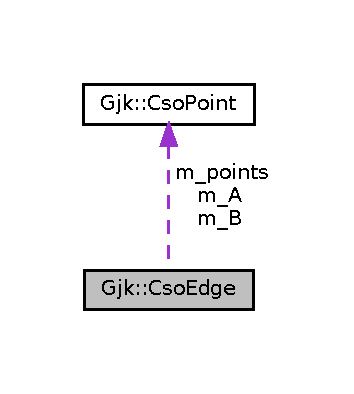
\includegraphics[width=170pt]{structGjk_1_1CsoEdge__coll__graph}
\end{center}
\end{figure}
\subsection*{Public Member Functions}
\begin{DoxyCompactItemize}
\item 
\mbox{\Hypertarget{structGjk_1_1CsoEdge_a8d9009b6a3943c070c62bbc826d5a83b}\label{structGjk_1_1CsoEdge_a8d9009b6a3943c070c62bbc826d5a83b}} 
{\bfseries Cso\+Edge} (const \hyperlink{structGjk_1_1CsoPoint}{Cso\+Point} \&a, const \hyperlink{structGjk_1_1CsoPoint}{Cso\+Point} \&b)
\end{DoxyCompactItemize}
\subsection*{Public Attributes}
\begin{DoxyCompactItemize}
\item 
\mbox{\Hypertarget{structGjk_1_1CsoEdge_a5e14c47961fc0f7e6a7fa03a2e997f40}\label{structGjk_1_1CsoEdge_a5e14c47961fc0f7e6a7fa03a2e997f40}} 
\begin{tabbing}
xx\=xx\=xx\=xx\=xx\=xx\=xx\=xx\=xx\=\kill
union \{\\
\mbox{\Hypertarget{unionGjk_1_1CsoEdge_1_1_0D18_a2ffa204621e9cb8c41b2be55e2974af0}\label{unionGjk_1_1CsoEdge_1_1_0D18_a2ffa204621e9cb8c41b2be55e2974af0}} 
\>struct \{\\
\>\>\hyperlink{structGjk_1_1CsoPoint}{CsoPoint} {\bfseries m\_A}\\
\>\>\hyperlink{structGjk_1_1CsoPoint}{CsoPoint} {\bfseries m\_B}\\
\>\} \\
\>\hyperlink{structGjk_1_1CsoPoint}{CsoPoint} {\bfseries m\_points} \mbox{[}2\mbox{]}\\
\}; \\

\end{tabbing}\end{DoxyCompactItemize}


The documentation for this struct was generated from the following files\+:\begin{DoxyCompactItemize}
\item 
Physics/\+Gjk/\hyperlink{Gjk_8h}{Gjk.\+h}\item 
Physics/\+Gjk/Gjk.\+cpp\end{DoxyCompactItemize}

\hypertarget{structGjk_1_1CsoPoint}{}\section{Gjk\+:\+:Cso\+Point Struct Reference}
\label{structGjk_1_1CsoPoint}\index{Gjk\+::\+Cso\+Point@{Gjk\+::\+Cso\+Point}}
\subsection*{Public Member Functions}
\begin{DoxyCompactItemize}
\item 
\mbox{\Hypertarget{structGjk_1_1CsoPoint_ad7e23024e0114e73d6978760a209782c}\label{structGjk_1_1CsoPoint_ad7e23024e0114e73d6978760a209782c}} 
bool {\bfseries operator==} (const \hyperlink{structGjk_1_1CsoPoint}{Cso\+Point} \&rhs) const
\end{DoxyCompactItemize}
\subsection*{Public Attributes}
\begin{DoxyCompactItemize}
\item 
\mbox{\Hypertarget{structGjk_1_1CsoPoint_ab6e2f2cde5e989b193061c6ba1362261}\label{structGjk_1_1CsoPoint_ab6e2f2cde5e989b193061c6ba1362261}} 
Vector3 {\bfseries m\+\_\+\+PointA}
\item 
\mbox{\Hypertarget{structGjk_1_1CsoPoint_a1fb66d7493641a43ffa4fc2e4efecdc2}\label{structGjk_1_1CsoPoint_a1fb66d7493641a43ffa4fc2e4efecdc2}} 
Vector3 {\bfseries m\+\_\+\+PointB}
\item 
\mbox{\Hypertarget{structGjk_1_1CsoPoint_ae9290f076800ece739001b3604018755}\label{structGjk_1_1CsoPoint_ae9290f076800ece739001b3604018755}} 
Vector3 {\bfseries m\+\_\+\+Cso\+Point}
\end{DoxyCompactItemize}


The documentation for this struct was generated from the following files\+:\begin{DoxyCompactItemize}
\item 
Physics/\+Gjk/\hyperlink{Gjk_8h}{Gjk.\+h}\item 
Physics/\+Gjk/Gjk.\+cpp\end{DoxyCompactItemize}

\hypertarget{structGjk_1_1CsoTriangle}{}\section{Gjk\+:\+:Cso\+Triangle Struct Reference}
\label{structGjk_1_1CsoTriangle}\index{Gjk\+::\+Cso\+Triangle@{Gjk\+::\+Cso\+Triangle}}


Collaboration diagram for Gjk\+:\+:Cso\+Triangle\+:\nopagebreak
\begin{figure}[H]
\begin{center}
\leavevmode
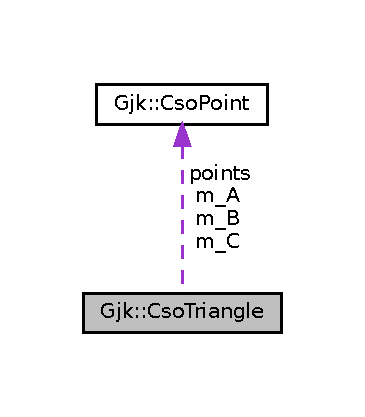
\includegraphics[width=175pt]{structGjk_1_1CsoTriangle__coll__graph}
\end{center}
\end{figure}
\subsection*{Public Member Functions}
\begin{DoxyCompactItemize}
\item 
\mbox{\Hypertarget{structGjk_1_1CsoTriangle_a16bd3105b189e3003fcc9cc27e57e90d}\label{structGjk_1_1CsoTriangle_a16bd3105b189e3003fcc9cc27e57e90d}} 
{\bfseries Cso\+Triangle} (const \hyperlink{structGjk_1_1CsoPoint}{Cso\+Point} \&a\+\_\+, const \hyperlink{structGjk_1_1CsoPoint}{Cso\+Point} \&b\+\_\+, const \hyperlink{structGjk_1_1CsoPoint}{Cso\+Point} \&c\+\_\+)
\end{DoxyCompactItemize}
\subsection*{Public Attributes}
\begin{DoxyCompactItemize}
\item 
\mbox{\Hypertarget{structGjk_1_1CsoTriangle_afc388c5a11f4edf9d95dde1e2baa1453}\label{structGjk_1_1CsoTriangle_afc388c5a11f4edf9d95dde1e2baa1453}} 
\begin{tabbing}
xx\=xx\=xx\=xx\=xx\=xx\=xx\=xx\=xx\=\kill
union \{\\
\mbox{\Hypertarget{unionGjk_1_1CsoTriangle_1_1_0D14_ab7b8f7296e9f94e1b6ed18b552cae39e}\label{unionGjk_1_1CsoTriangle_1_1_0D14_ab7b8f7296e9f94e1b6ed18b552cae39e}} 
\>struct \{\\
\>\>\hyperlink{structGjk_1_1CsoPoint}{CsoPoint} {\bfseries m\_A}\\
\>\>\hyperlink{structGjk_1_1CsoPoint}{CsoPoint} {\bfseries m\_B}\\
\>\>\hyperlink{structGjk_1_1CsoPoint}{CsoPoint} {\bfseries m\_C}\\
\>\} \\
\>\hyperlink{structGjk_1_1CsoPoint}{CsoPoint} {\bfseries points} \mbox{[}3\mbox{]}\\
\}; \\

\end{tabbing}\item 
\mbox{\Hypertarget{structGjk_1_1CsoTriangle_a328ee0494e17af474a8c9f524a15d8da}\label{structGjk_1_1CsoTriangle_a328ee0494e17af474a8c9f524a15d8da}} 
Vector3 {\bfseries m\+\_\+normal}
\end{DoxyCompactItemize}


The documentation for this struct was generated from the following files\+:\begin{DoxyCompactItemize}
\item 
Physics/\+Gjk/\hyperlink{Gjk_8h}{Gjk.\+h}\item 
Physics/\+Gjk/Gjk.\+cpp\end{DoxyCompactItemize}

\hypertarget{structCustomCompNode}{}\section{Custom\+Comp\+Node Struct Reference}
\label{structCustomCompNode}\index{Custom\+Comp\+Node@{Custom\+Comp\+Node}}


Inheritance diagram for Custom\+Comp\+Node\+:\nopagebreak
\begin{figure}[H]
\begin{center}
\leavevmode
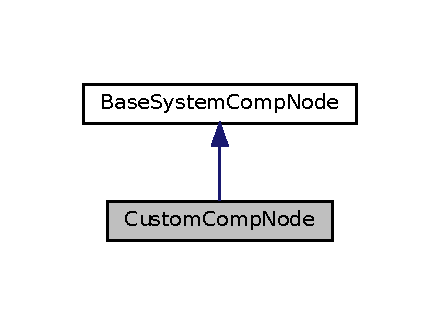
\includegraphics[width=211pt]{structCustomCompNode__inherit__graph}
\end{center}
\end{figure}


Collaboration diagram for Custom\+Comp\+Node\+:\nopagebreak
\begin{figure}[H]
\begin{center}
\leavevmode
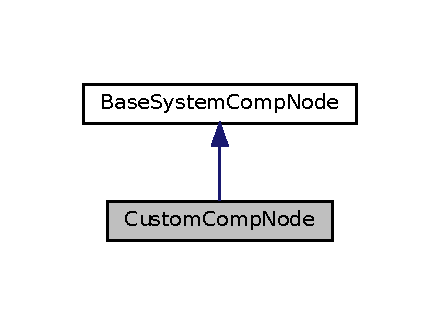
\includegraphics[width=211pt]{structCustomCompNode__coll__graph}
\end{center}
\end{figure}
\subsection*{Public Member Functions}
\begin{DoxyCompactItemize}
\item 
\mbox{\Hypertarget{structCustomCompNode_aad97992d43d962acbb3662a9af2a7d68}\label{structCustomCompNode_aad97992d43d962acbb3662a9af2a7d68}} 
{\bfseries Custom\+Comp\+Node} (std\+::vector$<$ \hyperlink{classCustomComponent}{Custom\+Component} $\ast$$>$ const \&comp\+List)
\end{DoxyCompactItemize}
\subsection*{Public Attributes}
\begin{DoxyCompactItemize}
\item 
\mbox{\Hypertarget{structCustomCompNode_a96e3609cd8ee658e78951d46e968ef49}\label{structCustomCompNode_a96e3609cd8ee658e78951d46e968ef49}} 
std\+::vector$<$ \hyperlink{classCustomComponent}{Custom\+Component} $\ast$ $>$ {\bfseries n\+\_\+components}
\end{DoxyCompactItemize}


The documentation for this struct was generated from the following file\+:\begin{DoxyCompactItemize}
\item 
Systems/\+Custom\+System/Custom\+System.\+h\end{DoxyCompactItemize}

\hypertarget{classCustomComponent}{}\section{Custom\+Component Class Reference}
\label{classCustomComponent}\index{Custom\+Component@{Custom\+Component}}


Class that represents the C\+PP class behind a scripted component.  




{\ttfamily \#include $<$Custom\+Component.\+h$>$}



Inheritance diagram for Custom\+Component\+:
\nopagebreak
\begin{figure}[H]
\begin{center}
\leavevmode
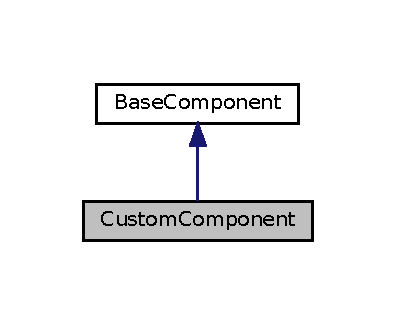
\includegraphics[width=190pt]{classCustomComponent__inherit__graph}
\end{center}
\end{figure}


Collaboration diagram for Custom\+Component\+:
\nopagebreak
\begin{figure}[H]
\begin{center}
\leavevmode
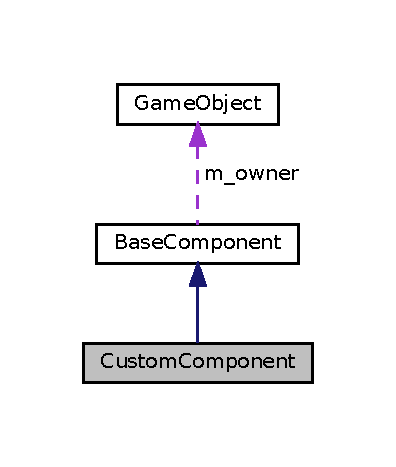
\includegraphics[width=190pt]{classCustomComponent__coll__graph}
\end{center}
\end{figure}
\subsection*{Public Member Functions}
\begin{DoxyCompactItemize}
\item 
\hyperlink{classCustomComponent_a748e48455ac06076251485d3a112140f}{Custom\+Component} (\hyperlink{classGameObject}{Game\+Object} $\ast$owner)
\begin{DoxyCompactList}\small\item\em Construct a new Custom Component object. \end{DoxyCompactList}\item 
\mbox{\Hypertarget{classCustomComponent_a79668a223e3efff11c27180ac90959c0}\label{classCustomComponent_a79668a223e3efff11c27180ac90959c0}} 
virtual \hyperlink{classCustomComponent_a79668a223e3efff11c27180ac90959c0}{$\sim$\+Custom\+Component} ()
\begin{DoxyCompactList}\small\item\em Destroy the Custom Component object. \end{DoxyCompactList}\item 
virtual void \hyperlink{classCustomComponent_a614f2af8f444be376d83cc00f6b9c7ea}{Init} (\hyperlink{classResourceManager}{Resource\+Manager} $\ast$res\+Mgr, \hyperlink{classDXRenderer}{D\+X\+Renderer} $\ast$dxrenderer) override
\begin{DoxyCompactList}\small\item\em Will do nothing on C\+PP other than call Init on the script. \end{DoxyCompactList}\item 
virtual void \hyperlink{classCustomComponent_a4c2ecd49242b844479cbee2e9385371b}{Begin} (\hyperlink{classGameObjectManager}{Game\+Object\+Manager} $\ast$go\+Mgr) override
\begin{DoxyCompactList}\small\item\em Will do nothing on C\+PP other than call Begin on the script. \end{DoxyCompactList}\item 
void \hyperlink{classCustomComponent_a938c6db19be64cb1d83da8f9ae7ba4d1}{Destroy} ()
\begin{DoxyCompactList}\small\item\em Will do nothing on C\+PP other than call Init on the script. \end{DoxyCompactList}\item 
\hyperlink{classStringId}{String\+Id} const  \& \hyperlink{classCustomComponent_aefb68297be52020412723f27a3c003f0}{Get\+Name} () const
\begin{DoxyCompactList}\small\item\em Get the Name of this scripted component (same name as script) \end{DoxyCompactList}\item 
sol\+::table \& \hyperlink{classCustomComponent_a5d59a3fcc75fbe18c2d2ab9d1fe76576}{get\+Custom\+Comp\+Lua\+Ref} ()
\begin{DoxyCompactList}\small\item\em Returns the lua table reference that corresponds to this Component\textquotesingle{}s script. \end{DoxyCompactList}\item 
void \hyperlink{classCustomComponent_ac540fc607bb502790276815b55890c98}{Script\+Setup} (\hyperlink{classStringId}{String\+Id} script\+Path, std\+::string const \&name, \hyperlink{classScriptingManager}{Scripting\+Manager} $\ast$lua\+Mgr)
\begin{DoxyCompactList}\small\item\em Sets the script up, by deep copying and getting the table reference from the \hyperlink{classScriptingManager}{Scripting\+Manager}. \end{DoxyCompactList}\item 
{\footnotesize template$<$typename T $>$ }\\void \hyperlink{classCustomComponent_ab3107db0a720c77d00f9b73060cbcef3}{Override} (std\+::string member, T value)
\begin{DoxyCompactList}\small\item\em Overrides a value on the script. Templatized since it can override different data types (as long as they exist on L\+UA) \end{DoxyCompactList}\end{DoxyCompactItemize}
\subsection*{Static Public Attributes}
\begin{DoxyCompactItemize}
\item 
\mbox{\Hypertarget{classCustomComponent_ae490cb396ab9ececc0a619a323929bfc}\label{classCustomComponent_ae490cb396ab9ececc0a619a323929bfc}} 
static Component\+Id const \hyperlink{classCustomComponent_ae490cb396ab9ececc0a619a323929bfc}{static\+\_\+type} = static\+\_\+cast$<$unsigned$>$(-\/1)
\begin{DoxyCompactList}\small\item\em Unique type identifier. \end{DoxyCompactList}\end{DoxyCompactItemize}
\subsection*{Friends}
\begin{DoxyCompactItemize}
\item 
\mbox{\Hypertarget{classCustomComponent_a328c093d609680cca505905c6d49901a}\label{classCustomComponent_a328c093d609680cca505905c6d49901a}} 
class {\bfseries Factory}
\item 
\mbox{\Hypertarget{classCustomComponent_ad53c39bc0891ebd13eca5e98a09ab765}\label{classCustomComponent_ad53c39bc0891ebd13eca5e98a09ab765}} 
class {\bfseries Custom\+System}
\item 
\mbox{\Hypertarget{classCustomComponent_ab3d6fafb2064bace492fd6b503d044f4}\label{classCustomComponent_ab3d6fafb2064bace492fd6b503d044f4}} 
class {\bfseries Scripting\+Manager}
\end{DoxyCompactItemize}
\subsection*{Additional Inherited Members}


\subsection{Detailed Description}
Class that represents the C\+PP class behind a scripted component. 

\subsection{Constructor \& Destructor Documentation}
\mbox{\Hypertarget{classCustomComponent_a748e48455ac06076251485d3a112140f}\label{classCustomComponent_a748e48455ac06076251485d3a112140f}} 
\index{Custom\+Component@{Custom\+Component}!Custom\+Component@{Custom\+Component}}
\index{Custom\+Component@{Custom\+Component}!Custom\+Component@{Custom\+Component}}
\subsubsection{\texorpdfstring{Custom\+Component()}{CustomComponent()}}
{\footnotesize\ttfamily Custom\+Component\+::\+Custom\+Component (\begin{DoxyParamCaption}\item[{\hyperlink{classGameObject}{Game\+Object} $\ast$}]{owner }\end{DoxyParamCaption})}



Construct a new Custom Component object. 


\begin{DoxyParams}{Parameters}
{\em owner} & \\
\hline
\end{DoxyParams}


\subsection{Member Function Documentation}
\mbox{\Hypertarget{classCustomComponent_a4c2ecd49242b844479cbee2e9385371b}\label{classCustomComponent_a4c2ecd49242b844479cbee2e9385371b}} 
\index{Custom\+Component@{Custom\+Component}!Begin@{Begin}}
\index{Begin@{Begin}!Custom\+Component@{Custom\+Component}}
\subsubsection{\texorpdfstring{Begin()}{Begin()}}
{\footnotesize\ttfamily void Custom\+Component\+::\+Begin (\begin{DoxyParamCaption}\item[{\hyperlink{classGameObjectManager}{Game\+Object\+Manager} $\ast$}]{go\+Mgr }\end{DoxyParamCaption})\hspace{0.3cm}{\ttfamily [override]}, {\ttfamily [virtual]}}



Will do nothing on C\+PP other than call Begin on the script. 


\begin{DoxyParams}{Parameters}
{\em go\+Mgr} & \\
\hline
\end{DoxyParams}


Implements \hyperlink{classBaseComponent}{Base\+Component}.

\mbox{\Hypertarget{classCustomComponent_a938c6db19be64cb1d83da8f9ae7ba4d1}\label{classCustomComponent_a938c6db19be64cb1d83da8f9ae7ba4d1}} 
\index{Custom\+Component@{Custom\+Component}!Destroy@{Destroy}}
\index{Destroy@{Destroy}!Custom\+Component@{Custom\+Component}}
\subsubsection{\texorpdfstring{Destroy()}{Destroy()}}
{\footnotesize\ttfamily void Custom\+Component\+::\+Destroy (\begin{DoxyParamCaption}{ }\end{DoxyParamCaption})}



Will do nothing on C\+PP other than call Init on the script. 


\begin{DoxyParams}{Parameters}
{\em res\+Mgr} & \\
\hline
{\em dxrenderer} & \\
\hline
\end{DoxyParams}
\mbox{\Hypertarget{classCustomComponent_a5d59a3fcc75fbe18c2d2ab9d1fe76576}\label{classCustomComponent_a5d59a3fcc75fbe18c2d2ab9d1fe76576}} 
\index{Custom\+Component@{Custom\+Component}!get\+Custom\+Comp\+Lua\+Ref@{get\+Custom\+Comp\+Lua\+Ref}}
\index{get\+Custom\+Comp\+Lua\+Ref@{get\+Custom\+Comp\+Lua\+Ref}!Custom\+Component@{Custom\+Component}}
\subsubsection{\texorpdfstring{get\+Custom\+Comp\+Lua\+Ref()}{getCustomCompLuaRef()}}
{\footnotesize\ttfamily sol\+::table \& Custom\+Component\+::get\+Custom\+Comp\+Lua\+Ref (\begin{DoxyParamCaption}{ }\end{DoxyParamCaption})}



Returns the lua table reference that corresponds to this Component\textquotesingle{}s script. 

\begin{DoxyReturn}{Returns}
sol\+::table\& 
\end{DoxyReturn}
\mbox{\Hypertarget{classCustomComponent_aefb68297be52020412723f27a3c003f0}\label{classCustomComponent_aefb68297be52020412723f27a3c003f0}} 
\index{Custom\+Component@{Custom\+Component}!Get\+Name@{Get\+Name}}
\index{Get\+Name@{Get\+Name}!Custom\+Component@{Custom\+Component}}
\subsubsection{\texorpdfstring{Get\+Name()}{GetName()}}
{\footnotesize\ttfamily \hyperlink{classStringId}{String\+Id} const  \& Custom\+Component\+::\+Get\+Name (\begin{DoxyParamCaption}{ }\end{DoxyParamCaption}) const}



Get the Name of this scripted component (same name as script) 

\begin{DoxyReturn}{Returns}
\hyperlink{classStringId}{String\+Id} const\& 
\end{DoxyReturn}
\mbox{\Hypertarget{classCustomComponent_a614f2af8f444be376d83cc00f6b9c7ea}\label{classCustomComponent_a614f2af8f444be376d83cc00f6b9c7ea}} 
\index{Custom\+Component@{Custom\+Component}!Init@{Init}}
\index{Init@{Init}!Custom\+Component@{Custom\+Component}}
\subsubsection{\texorpdfstring{Init()}{Init()}}
{\footnotesize\ttfamily void Custom\+Component\+::\+Init (\begin{DoxyParamCaption}\item[{\hyperlink{classResourceManager}{Resource\+Manager} $\ast$}]{res\+Mgr,  }\item[{\hyperlink{classDXRenderer}{D\+X\+Renderer} $\ast$}]{dxrenderer }\end{DoxyParamCaption})\hspace{0.3cm}{\ttfamily [override]}, {\ttfamily [virtual]}}



Will do nothing on C\+PP other than call Init on the script. 


\begin{DoxyParams}{Parameters}
{\em res\+Mgr} & \\
\hline
{\em dxrenderer} & \\
\hline
\end{DoxyParams}


Implements \hyperlink{classBaseComponent}{Base\+Component}.

\mbox{\Hypertarget{classCustomComponent_ab3107db0a720c77d00f9b73060cbcef3}\label{classCustomComponent_ab3107db0a720c77d00f9b73060cbcef3}} 
\index{Custom\+Component@{Custom\+Component}!Override@{Override}}
\index{Override@{Override}!Custom\+Component@{Custom\+Component}}
\subsubsection{\texorpdfstring{Override()}{Override()}}
{\footnotesize\ttfamily template$<$typename T $>$ \\
void Custom\+Component\+::\+Override (\begin{DoxyParamCaption}\item[{std\+::string}]{member,  }\item[{T}]{value }\end{DoxyParamCaption})}



Overrides a value on the script. Templatized since it can override different data types (as long as they exist on L\+UA) 


\begin{DoxyTemplParams}{Template Parameters}
{\em T} & \\
\hline
\end{DoxyTemplParams}

\begin{DoxyParams}{Parameters}
{\em member} & \\
\hline
{\em value} & \\
\hline
\end{DoxyParams}
\mbox{\Hypertarget{classCustomComponent_ac540fc607bb502790276815b55890c98}\label{classCustomComponent_ac540fc607bb502790276815b55890c98}} 
\index{Custom\+Component@{Custom\+Component}!Script\+Setup@{Script\+Setup}}
\index{Script\+Setup@{Script\+Setup}!Custom\+Component@{Custom\+Component}}
\subsubsection{\texorpdfstring{Script\+Setup()}{ScriptSetup()}}
{\footnotesize\ttfamily void Custom\+Component\+::\+Script\+Setup (\begin{DoxyParamCaption}\item[{\hyperlink{classStringId}{String\+Id}}]{script\+Path,  }\item[{std\+::string const \&}]{name,  }\item[{\hyperlink{classScriptingManager}{Scripting\+Manager} $\ast$}]{lua\+Mgr }\end{DoxyParamCaption})}



Sets the script up, by deep copying and getting the table reference from the \hyperlink{classScriptingManager}{Scripting\+Manager}. 


\begin{DoxyParams}{Parameters}
{\em script\+Path} & \\
\hline
{\em name} & \\
\hline
{\em lua\+Mgr} & \\
\hline
\end{DoxyParams}
m\+\_\+lua\+Script\+Table\mbox{[}\char`\"{}\+Get\+Owner\char`\"{}\mbox{]} = \&\hyperlink{classBaseComponent_aa07f9b9c2ebdd2c314404771857e9e07}{Custom\+Component\+::\+Get\+Owner}; m\+\_\+lua\+Script\+Table\mbox{[}\char`\"{}\+Get\+Name\char`\"{}\mbox{]} = \&\hyperlink{classCustomComponent_aefb68297be52020412723f27a3c003f0}{Custom\+Component\+::\+Get\+Name}; 

The documentation for this class was generated from the following files\+:\begin{DoxyCompactItemize}
\item 
Components/\+Custom\+Component/\hyperlink{CustomComponent_8h}{Custom\+Component.\+h}\item 
Components/\+Custom\+Component/Custom\+Component.\+cpp\end{DoxyCompactItemize}

\hypertarget{classCustomSystem}{}\section{Custom\+System Class Reference}
\label{classCustomSystem}\index{Custom\+System@{Custom\+System}}


System that handles Update for the scripted component of Game\+Objects.  




{\ttfamily \#include $<$Custom\+System.\+h$>$}



Inheritance diagram for Custom\+System\+:
\nopagebreak
\begin{figure}[H]
\begin{center}
\leavevmode
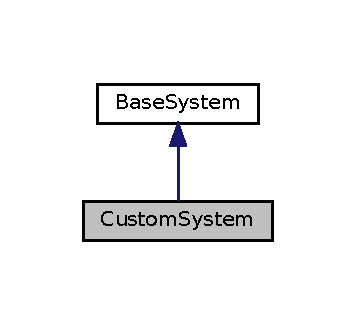
\includegraphics[width=171pt]{classCustomSystem__inherit__graph}
\end{center}
\end{figure}


Collaboration diagram for Custom\+System\+:
\nopagebreak
\begin{figure}[H]
\begin{center}
\leavevmode
\includegraphics[width=171pt]{classCustomSystem__coll__graph}
\end{center}
\end{figure}
\subsection*{Public Member Functions}
\begin{DoxyCompactItemize}
\item 
\mbox{\Hypertarget{classCustomSystem_a452aafe02e3b43713a732d2457c271c4}\label{classCustomSystem_a452aafe02e3b43713a732d2457c271c4}} 
\hyperlink{classCustomSystem_a452aafe02e3b43713a732d2457c271c4}{Custom\+System} ()
\begin{DoxyCompactList}\small\item\em Construct a new Custom System object. \end{DoxyCompactList}\item 
\mbox{\Hypertarget{classCustomSystem_a7426abb7e961d7eb28ead6af07f751cd}\label{classCustomSystem_a7426abb7e961d7eb28ead6af07f751cd}} 
virtual \hyperlink{classCustomSystem_a7426abb7e961d7eb28ead6af07f751cd}{$\sim$\+Custom\+System} ()
\begin{DoxyCompactList}\small\item\em Destroy the Custom System object. \end{DoxyCompactList}\item 
virtual void \hyperlink{classCustomSystem_a1fe5c399dec16f2a8aff1a5c9e06760e}{Register\+\_\+\+Game\+Object} (\hyperlink{classGameObject}{Game\+Object} $\ast$go)
\begin{DoxyCompactList}\small\item\em Registers a \hyperlink{classGameObject}{Game\+Object} onto this system. Only Game\+Objects with custom components can register. \end{DoxyCompactList}\item 
virtual void \hyperlink{classCustomSystem_ab8b072ffd6b4de7404b385068d735c61}{Update} (float dt, \hyperlink{structBaseSystemCompNode}{Base\+System\+Comp\+Node} $\ast$comp\+Node)
\begin{DoxyCompactList}\small\item\em Calls update on all the scripts of the Game\+Objects registered with this system. \end{DoxyCompactList}\item 
virtual void \hyperlink{classCustomSystem_a6552a2339d179ca963650e94ee1bf615}{Draw} (float dt, \hyperlink{structBaseSystemCompNode}{Base\+System\+Comp\+Node} $\ast$comp\+Node) override
\begin{DoxyCompactList}\small\item\em Calls draw on all the scripts of the Game\+Objects registered with this system. \end{DoxyCompactList}\item 
\mbox{\Hypertarget{classCustomSystem_aee254ef81ede23cbbfc18ade88d9dcc5}\label{classCustomSystem_aee254ef81ede23cbbfc18ade88d9dcc5}} 
void {\bfseries Register\+App\+Renderer} (\hyperlink{classAppRenderer}{App\+Renderer} $\ast$app\+Renderer)
\end{DoxyCompactItemize}
\subsection*{Static Public Attributes}
\begin{DoxyCompactItemize}
\item 
\mbox{\Hypertarget{classCustomSystem_a1c3d97bf73201a0c3e1c306440ff94a7}\label{classCustomSystem_a1c3d97bf73201a0c3e1c306440ff94a7}} 
static unsigned int const \hyperlink{classCustomSystem_a1c3d97bf73201a0c3e1c306440ff94a7}{static\+\_\+type} = \hyperlink{classBaseSystem_a7ef356edab3cfb02905e0a73a645b131}{Base\+System\+::number\+Of\+Types}++
\begin{DoxyCompactList}\small\item\em To compare when using templates. \end{DoxyCompactList}\end{DoxyCompactItemize}
\subsection*{Friends}
\begin{DoxyCompactItemize}
\item 
\mbox{\Hypertarget{classCustomSystem_a328c093d609680cca505905c6d49901a}\label{classCustomSystem_a328c093d609680cca505905c6d49901a}} 
class {\bfseries Factory}
\end{DoxyCompactItemize}
\subsection*{Additional Inherited Members}


\subsection{Detailed Description}
System that handles Update for the scripted component of Game\+Objects. 

\subsection{Member Function Documentation}
\mbox{\Hypertarget{classCustomSystem_a6552a2339d179ca963650e94ee1bf615}\label{classCustomSystem_a6552a2339d179ca963650e94ee1bf615}} 
\index{Custom\+System@{Custom\+System}!Draw@{Draw}}
\index{Draw@{Draw}!Custom\+System@{Custom\+System}}
\subsubsection{\texorpdfstring{Draw()}{Draw()}}
{\footnotesize\ttfamily void Custom\+System\+::\+Draw (\begin{DoxyParamCaption}\item[{float}]{dt,  }\item[{\hyperlink{structBaseSystemCompNode}{Base\+System\+Comp\+Node} $\ast$}]{comp\+Node }\end{DoxyParamCaption})\hspace{0.3cm}{\ttfamily [override]}, {\ttfamily [virtual]}}



Calls draw on all the scripts of the Game\+Objects registered with this system. 


\begin{DoxyParams}{Parameters}
{\em comp\+Node} & \\
\hline
\end{DoxyParams}


Reimplemented from \hyperlink{classBaseSystem_a94339337789820c707da572d140a0923}{Base\+System}.

\mbox{\Hypertarget{classCustomSystem_a1fe5c399dec16f2a8aff1a5c9e06760e}\label{classCustomSystem_a1fe5c399dec16f2a8aff1a5c9e06760e}} 
\index{Custom\+System@{Custom\+System}!Register\+\_\+\+Game\+Object@{Register\+\_\+\+Game\+Object}}
\index{Register\+\_\+\+Game\+Object@{Register\+\_\+\+Game\+Object}!Custom\+System@{Custom\+System}}
\subsubsection{\texorpdfstring{Register\+\_\+\+Game\+Object()}{Register\_GameObject()}}
{\footnotesize\ttfamily void Custom\+System\+::\+Register\+\_\+\+Game\+Object (\begin{DoxyParamCaption}\item[{\hyperlink{classGameObject}{Game\+Object} $\ast$}]{go }\end{DoxyParamCaption})\hspace{0.3cm}{\ttfamily [virtual]}}



Registers a \hyperlink{classGameObject}{Game\+Object} onto this system. Only Game\+Objects with custom components can register. 


\begin{DoxyParams}{Parameters}
{\em go} & \\
\hline
\end{DoxyParams}


Implements \hyperlink{classBaseSystem}{Base\+System}.

\mbox{\Hypertarget{classCustomSystem_ab8b072ffd6b4de7404b385068d735c61}\label{classCustomSystem_ab8b072ffd6b4de7404b385068d735c61}} 
\index{Custom\+System@{Custom\+System}!Update@{Update}}
\index{Update@{Update}!Custom\+System@{Custom\+System}}
\subsubsection{\texorpdfstring{Update()}{Update()}}
{\footnotesize\ttfamily void Custom\+System\+::\+Update (\begin{DoxyParamCaption}\item[{float}]{dt,  }\item[{\hyperlink{structBaseSystemCompNode}{Base\+System\+Comp\+Node} $\ast$}]{comp\+Node }\end{DoxyParamCaption})\hspace{0.3cm}{\ttfamily [virtual]}}



Calls update on all the scripts of the Game\+Objects registered with this system. 


\begin{DoxyParams}{Parameters}
{\em dt} & \\
\hline
{\em comp\+Node} & \\
\hline
\end{DoxyParams}


Reimplemented from \hyperlink{classBaseSystem_a465191589a1ef8b8f3a8e20fa4656d47}{Base\+System}.



The documentation for this class was generated from the following files\+:\begin{DoxyCompactItemize}
\item 
Systems/\+Custom\+System/\hyperlink{CustomSystem_8h}{Custom\+System.\+h}\item 
Systems/\+Custom\+System/Custom\+System.\+cpp\end{DoxyCompactItemize}

\hypertarget{structDebugAABBInstance}{}\section{Debug\+A\+A\+B\+B\+Instance Struct Reference}
\label{structDebugAABBInstance}\index{Debug\+A\+A\+B\+B\+Instance@{Debug\+A\+A\+B\+B\+Instance}}
\subsection*{Public Attributes}
\begin{DoxyCompactItemize}
\item 
\mbox{\Hypertarget{structDebugAABBInstance_a70c7226d27e3102495319048155b0e82}\label{structDebugAABBInstance_a70c7226d27e3102495319048155b0e82}} 
Vector3 {\bfseries m\+\_\+min\+\_\+bound}
\item 
\mbox{\Hypertarget{structDebugAABBInstance_a047247555ac7f24886e8beb075959ec3}\label{structDebugAABBInstance_a047247555ac7f24886e8beb075959ec3}} 
Vector3 {\bfseries m\+\_\+max\+\_\+bound}
\item 
\mbox{\Hypertarget{structDebugAABBInstance_abf825faaf4d681142ed7ce2e86fb7d7e}\label{structDebugAABBInstance_abf825faaf4d681142ed7ce2e86fb7d7e}} 
Vector3 {\bfseries m\+\_\+color}
\end{DoxyCompactItemize}


The documentation for this struct was generated from the following file\+:\begin{DoxyCompactItemize}
\item 
Graphics/\+Debug\+Rendering/Debug\+Rendering.\+h\end{DoxyCompactItemize}

\hypertarget{structDebugInstanceUniformData}{}\section{Debug\+Instance\+Uniform\+Data Struct Reference}
\label{structDebugInstanceUniformData}\index{Debug\+Instance\+Uniform\+Data@{Debug\+Instance\+Uniform\+Data}}
\subsection*{Public Attributes}
\begin{DoxyCompactItemize}
\item 
\mbox{\Hypertarget{structDebugInstanceUniformData_aaa53a25ae8a11a1fff82b2f6010178ed}\label{structDebugInstanceUniformData_aaa53a25ae8a11a1fff82b2f6010178ed}} 
float4x4 {\bfseries Model\+View\+Projection\+Mat}
\item 
\mbox{\Hypertarget{structDebugInstanceUniformData_ac8a706eeff4a11a9e9d4a8115562550a}\label{structDebugInstanceUniformData_ac8a706eeff4a11a9e9d4a8115562550a}} 
float4 {\bfseries Color}
\end{DoxyCompactItemize}


The documentation for this struct was generated from the following file\+:\begin{DoxyCompactItemize}
\item 
Shaders/Shading.\+h\end{DoxyCompactItemize}

\hypertarget{structDebugLineInstance}{}\section{Debug\+Line\+Instance Struct Reference}
\label{structDebugLineInstance}\index{Debug\+Line\+Instance@{Debug\+Line\+Instance}}
\subsection*{Public Attributes}
\begin{DoxyCompactItemize}
\item 
\mbox{\Hypertarget{structDebugLineInstance_aa1732db51793115864aa41688840c358}\label{structDebugLineInstance_aa1732db51793115864aa41688840c358}} 
Vector3 {\bfseries m\+\_\+startpos}
\item 
\mbox{\Hypertarget{structDebugLineInstance_a41c27823edb10afec6f616a57adcf562}\label{structDebugLineInstance_a41c27823edb10afec6f616a57adcf562}} 
Vector3 {\bfseries m\+\_\+endpos}
\item 
\mbox{\Hypertarget{structDebugLineInstance_ad361db9b353f1faf16b0b5a197431535}\label{structDebugLineInstance_ad361db9b353f1faf16b0b5a197431535}} 
Vector3 {\bfseries m\+\_\+color}
\end{DoxyCompactItemize}


The documentation for this struct was generated from the following file\+:\begin{DoxyCompactItemize}
\item 
Graphics/\+Debug\+Rendering/Debug\+Rendering.\+h\end{DoxyCompactItemize}

\hypertarget{classDebugRendering}{}\section{Debug\+Rendering Class Reference}
\label{classDebugRendering}\index{Debug\+Rendering@{Debug\+Rendering}}


The high level debug rendering interfaces.  




{\ttfamily \#include $<$Debug\+Rendering.\+h$>$}

\subsection*{Public Types}
\begin{DoxyCompactItemize}
\item 
\mbox{\Hypertarget{classDebugRendering_ae09e1ad33f1ba1575544cf3c70769ecc}\label{classDebugRendering_ae09e1ad33f1ba1575544cf3c70769ecc}} 
typedef std\+::vector$<$ \hyperlink{structDebugAABBInstance}{Debug\+A\+A\+B\+B\+Instance} $>$ {\bfseries Debug\+A\+A\+B\+B\+Instance\+List}
\item 
\mbox{\Hypertarget{classDebugRendering_a0dabb4da850186ab6f981b00723834e7}\label{classDebugRendering_a0dabb4da850186ab6f981b00723834e7}} 
typedef std\+::vector$<$ \hyperlink{structDebugSphereInstance}{Debug\+Sphere\+Instance} $>$ {\bfseries Debug\+Sphere\+Instance\+List}
\item 
\mbox{\Hypertarget{classDebugRendering_a45d525d5ab2cde6b7bceaf070dd6326a}\label{classDebugRendering_a45d525d5ab2cde6b7bceaf070dd6326a}} 
typedef std\+::vector$<$ \hyperlink{structDebugLineInstance}{Debug\+Line\+Instance} $>$ {\bfseries Debug\+Line\+Instance\+List}
\end{DoxyCompactItemize}
\subsection*{Public Member Functions}
\begin{DoxyCompactItemize}
\item 
\mbox{\Hypertarget{classDebugRendering_a04ef1665968e635ed878172cd43cd2ed}\label{classDebugRendering_a04ef1665968e635ed878172cd43cd2ed}} 
{\bfseries Debug\+Rendering} (\hyperlink{classAppRenderer}{App\+Renderer} $\ast$app\+\_\+renderer, \hyperlink{classResourceManager}{Resource\+Manager} $\ast$resource\+Manager)
\item 
\mbox{\Hypertarget{classDebugRendering_ab45f169c9f87018d13765d9949bba9c3}\label{classDebugRendering_ab45f169c9f87018d13765d9949bba9c3}} 
void {\bfseries Update\+Debug\+Uniform\+Buffer} ()
\item 
\mbox{\Hypertarget{classDebugRendering_ac6297a659a130d3e430c403faa608407}\label{classDebugRendering_ac6297a659a130d3e430c403faa608407}} 
void \hyperlink{classDebugRendering_ac6297a659a130d3e430c403faa608407}{Release} ()
\begin{DoxyCompactList}\small\item\em Release all graphics resources related to debug rendering. \end{DoxyCompactList}\item 
void \hyperlink{classDebugRendering_a4d86a142ed880456dbc732d213cc93e1}{Register\+Debug\+Line\+Instance} (const Vector3 \&start\+\_\+pos, const Vector3 \&end\+\_\+pos, const Vector3 \&color)
\begin{DoxyCompactList}\small\item\em Send render info request for debug line drawing. \end{DoxyCompactList}\item 
void \hyperlink{classDebugRendering_a9e23739719cbe569a0afefa6bb203330}{Register\+Debug\+Line\+Instance} (const \hyperlink{structDebugLineInstance}{Debug\+Line\+Instance} \&line\+\_\+instance)
\begin{DoxyCompactList}\small\item\em Send render info request for debug line drawing. \end{DoxyCompactList}\item 
void \hyperlink{classDebugRendering_a19e4cb443e7b0959dfd427431009acc4}{Register\+Debug\+A\+A\+BB} (const \hyperlink{structDebugAABBInstance}{Debug\+A\+A\+B\+B\+Instance} \&debug\+\_\+aabb\+\_\+instance)
\begin{DoxyCompactList}\small\item\em Send render info request for wireframe debug A\+A\+BB drawing. \end{DoxyCompactList}\item 
void \hyperlink{classDebugRendering_a43b18f36eff07b60f7dcace9549c126b}{Register\+Debug\+Sphere} (const \hyperlink{structDebugSphereInstance}{Debug\+Sphere\+Instance} \&debug\+\_\+sphere\+\_\+instance)
\begin{DoxyCompactList}\small\item\em Send render info request for wireframe debug sphere drawing. \end{DoxyCompactList}\item 
void \hyperlink{classDebugRendering_acdce8201c1a8f304b70bf278fd7b9cdb}{Update} (float dt)
\begin{DoxyCompactList}\small\item\em Update debug rendering logic. \end{DoxyCompactList}\item 
void \hyperlink{classDebugRendering_a2b3fd46f7880bcf6a57eb1b3af5dbc6d}{Load\+Content} (\hyperlink{classDXRenderer}{D\+X\+Renderer} $\ast$dxrenderer)
\begin{DoxyCompactList}\small\item\em Load all high level resources related to debug rendering. \end{DoxyCompactList}\item 
\mbox{\Hypertarget{classDebugRendering_a9251ff1132aa73c074d369ddb6d7ab03}\label{classDebugRendering_a9251ff1132aa73c074d369ddb6d7ab03}} 
void \hyperlink{classDebugRendering_a9251ff1132aa73c074d369ddb6d7ab03}{Clear\+Instances} ()
\begin{DoxyCompactList}\small\item\em Clear all the debug render info request. \end{DoxyCompactList}\end{DoxyCompactItemize}
\subsection*{Friends}
\begin{DoxyCompactItemize}
\item 
\mbox{\Hypertarget{classDebugRendering_aa2fce3a4ae64b69f01e0fd64ba26023a}\label{classDebugRendering_aa2fce3a4ae64b69f01e0fd64ba26023a}} 
class {\bfseries Debug\+Rendering\+Instance}
\end{DoxyCompactItemize}


\subsection{Detailed Description}
The high level debug rendering interfaces. 

\subsection{Member Function Documentation}
\mbox{\Hypertarget{classDebugRendering_a2b3fd46f7880bcf6a57eb1b3af5dbc6d}\label{classDebugRendering_a2b3fd46f7880bcf6a57eb1b3af5dbc6d}} 
\index{Debug\+Rendering@{Debug\+Rendering}!Load\+Content@{Load\+Content}}
\index{Load\+Content@{Load\+Content}!Debug\+Rendering@{Debug\+Rendering}}
\subsubsection{\texorpdfstring{Load\+Content()}{LoadContent()}}
{\footnotesize\ttfamily void Debug\+Rendering\+::\+Load\+Content (\begin{DoxyParamCaption}\item[{\hyperlink{classDXRenderer}{D\+X\+Renderer} $\ast$}]{dxrenderer }\end{DoxyParamCaption})}



Load all high level resources related to debug rendering. 


\begin{DoxyParams}{Parameters}
{\em dxrenderer} & \\
\hline
\end{DoxyParams}
\mbox{\Hypertarget{classDebugRendering_a19e4cb443e7b0959dfd427431009acc4}\label{classDebugRendering_a19e4cb443e7b0959dfd427431009acc4}} 
\index{Debug\+Rendering@{Debug\+Rendering}!Register\+Debug\+A\+A\+BB@{Register\+Debug\+A\+A\+BB}}
\index{Register\+Debug\+A\+A\+BB@{Register\+Debug\+A\+A\+BB}!Debug\+Rendering@{Debug\+Rendering}}
\subsubsection{\texorpdfstring{Register\+Debug\+A\+A\+B\+B()}{RegisterDebugAABB()}}
{\footnotesize\ttfamily void Debug\+Rendering\+::\+Register\+Debug\+A\+A\+BB (\begin{DoxyParamCaption}\item[{const \hyperlink{structDebugAABBInstance}{Debug\+A\+A\+B\+B\+Instance} \&}]{debug\+\_\+aabb\+\_\+instance }\end{DoxyParamCaption})}



Send render info request for wireframe debug A\+A\+BB drawing. 


\begin{DoxyParams}{Parameters}
{\em debug\+\_\+aabb\+\_\+instance} & \\
\hline
\end{DoxyParams}
\mbox{\Hypertarget{classDebugRendering_a4d86a142ed880456dbc732d213cc93e1}\label{classDebugRendering_a4d86a142ed880456dbc732d213cc93e1}} 
\index{Debug\+Rendering@{Debug\+Rendering}!Register\+Debug\+Line\+Instance@{Register\+Debug\+Line\+Instance}}
\index{Register\+Debug\+Line\+Instance@{Register\+Debug\+Line\+Instance}!Debug\+Rendering@{Debug\+Rendering}}
\subsubsection{\texorpdfstring{Register\+Debug\+Line\+Instance()}{RegisterDebugLineInstance()}\hspace{0.1cm}{\footnotesize\ttfamily [1/2]}}
{\footnotesize\ttfamily void Debug\+Rendering\+::\+Register\+Debug\+Line\+Instance (\begin{DoxyParamCaption}\item[{const Vector3 \&}]{start\+\_\+pos,  }\item[{const Vector3 \&}]{end\+\_\+pos,  }\item[{const Vector3 \&}]{color }\end{DoxyParamCaption})}



Send render info request for debug line drawing. 


\begin{DoxyParams}{Parameters}
{\em start\+\_\+pos} & \\
\hline
{\em end\+\_\+pos} & \\
\hline
{\em color} & \\
\hline
\end{DoxyParams}
\mbox{\Hypertarget{classDebugRendering_a9e23739719cbe569a0afefa6bb203330}\label{classDebugRendering_a9e23739719cbe569a0afefa6bb203330}} 
\index{Debug\+Rendering@{Debug\+Rendering}!Register\+Debug\+Line\+Instance@{Register\+Debug\+Line\+Instance}}
\index{Register\+Debug\+Line\+Instance@{Register\+Debug\+Line\+Instance}!Debug\+Rendering@{Debug\+Rendering}}
\subsubsection{\texorpdfstring{Register\+Debug\+Line\+Instance()}{RegisterDebugLineInstance()}\hspace{0.1cm}{\footnotesize\ttfamily [2/2]}}
{\footnotesize\ttfamily void Debug\+Rendering\+::\+Register\+Debug\+Line\+Instance (\begin{DoxyParamCaption}\item[{const \hyperlink{structDebugLineInstance}{Debug\+Line\+Instance} \&}]{line\+\_\+instance }\end{DoxyParamCaption})}



Send render info request for debug line drawing. 


\begin{DoxyParams}{Parameters}
{\em line\+\_\+instance} & \\
\hline
\end{DoxyParams}
\mbox{\Hypertarget{classDebugRendering_a43b18f36eff07b60f7dcace9549c126b}\label{classDebugRendering_a43b18f36eff07b60f7dcace9549c126b}} 
\index{Debug\+Rendering@{Debug\+Rendering}!Register\+Debug\+Sphere@{Register\+Debug\+Sphere}}
\index{Register\+Debug\+Sphere@{Register\+Debug\+Sphere}!Debug\+Rendering@{Debug\+Rendering}}
\subsubsection{\texorpdfstring{Register\+Debug\+Sphere()}{RegisterDebugSphere()}}
{\footnotesize\ttfamily void Debug\+Rendering\+::\+Register\+Debug\+Sphere (\begin{DoxyParamCaption}\item[{const \hyperlink{structDebugSphereInstance}{Debug\+Sphere\+Instance} \&}]{debug\+\_\+sphere\+\_\+instance }\end{DoxyParamCaption})}



Send render info request for wireframe debug sphere drawing. 


\begin{DoxyParams}{Parameters}
{\em debug\+\_\+sphere\+\_\+instance} & \\
\hline
\end{DoxyParams}
\mbox{\Hypertarget{classDebugRendering_acdce8201c1a8f304b70bf278fd7b9cdb}\label{classDebugRendering_acdce8201c1a8f304b70bf278fd7b9cdb}} 
\index{Debug\+Rendering@{Debug\+Rendering}!Update@{Update}}
\index{Update@{Update}!Debug\+Rendering@{Debug\+Rendering}}
\subsubsection{\texorpdfstring{Update()}{Update()}}
{\footnotesize\ttfamily void Debug\+Rendering\+::\+Update (\begin{DoxyParamCaption}\item[{float}]{dt }\end{DoxyParamCaption})}



Update debug rendering logic. 


\begin{DoxyParams}{Parameters}
{\em dt} & \\
\hline
\end{DoxyParams}


The documentation for this class was generated from the following files\+:\begin{DoxyCompactItemize}
\item 
Graphics/\+Debug\+Rendering/\hyperlink{DebugRendering_8h}{Debug\+Rendering.\+h}\item 
Graphics/\+Debug\+Rendering/Debug\+Rendering.\+cpp\end{DoxyCompactItemize}

\hypertarget{classDebugRenderingInstance}{}\section{Debug\+Rendering\+Instance Class Reference}
\label{classDebugRenderingInstance}\index{Debug\+Rendering\+Instance@{Debug\+Rendering\+Instance}}
\subsection*{Public Member Functions}
\begin{DoxyCompactItemize}
\item 
\mbox{\Hypertarget{classDebugRenderingInstance_ad0a7f7c1835296c93c888f899e54d181}\label{classDebugRenderingInstance_ad0a7f7c1835296c93c888f899e54d181}} 
{\bfseries Debug\+Rendering\+Instance} (\hyperlink{classDebugRendering}{Debug\+Rendering} \&debug\+Rendering)
\item 
\mbox{\Hypertarget{classDebugRenderingInstance_a10ae7e020d9cbf96a0f75c51a4e1ca92}\label{classDebugRenderingInstance_a10ae7e020d9cbf96a0f75c51a4e1ca92}} 
void {\bfseries Update} (const \hyperlink{structAppRendererContext}{App\+Renderer\+Context} \&app\+Renderer\+Context, float dt)
\item 
\mbox{\Hypertarget{classDebugRenderingInstance_ab5ba2696c823b156cc41fa41480b6076}\label{classDebugRenderingInstance_ab5ba2696c823b156cc41fa41480b6076}} 
void {\bfseries Render} (const \hyperlink{structAppRendererContext}{App\+Renderer\+Context} \&app\+Renderer\+Context)
\item 
\mbox{\Hypertarget{classDebugRenderingInstance_a5fa8f530c75e15869550bdf8d6814302}\label{classDebugRenderingInstance_a5fa8f530c75e15869550bdf8d6814302}} 
void {\bfseries Initialize} ()
\item 
\mbox{\Hypertarget{classDebugRenderingInstance_ace67dea54e2b930f9c3a0faabf154163}\label{classDebugRenderingInstance_ace67dea54e2b930f9c3a0faabf154163}} 
void {\bfseries Load\+Content} ()
\item 
\mbox{\Hypertarget{classDebugRenderingInstance_a02154ca8f49fa0e80900e4e05f4a48e9}\label{classDebugRenderingInstance_a02154ca8f49fa0e80900e4e05f4a48e9}} 
void {\bfseries Release} ()
\end{DoxyCompactItemize}


The documentation for this class was generated from the following files\+:\begin{DoxyCompactItemize}
\item 
Graphics/\+Debug\+Rendering/Debug\+Rendering\+Instance.\+h\item 
Graphics/\+Debug\+Rendering/Debug\+Rendering\+Instance.\+cpp\end{DoxyCompactItemize}

\hypertarget{structDebugSphereInstance}{}\section{Debug\+Sphere\+Instance Struct Reference}
\label{structDebugSphereInstance}\index{Debug\+Sphere\+Instance@{Debug\+Sphere\+Instance}}
\subsection*{Public Attributes}
\begin{DoxyCompactItemize}
\item 
\mbox{\Hypertarget{structDebugSphereInstance_af998ca53b90737be1b18db99e7f09da9}\label{structDebugSphereInstance_af998ca53b90737be1b18db99e7f09da9}} 
Vector3 {\bfseries m\+\_\+center}
\item 
\mbox{\Hypertarget{structDebugSphereInstance_afde262deb97af3cb282f3d917daad640}\label{structDebugSphereInstance_afde262deb97af3cb282f3d917daad640}} 
float {\bfseries m\+\_\+radius}
\item 
\mbox{\Hypertarget{structDebugSphereInstance_a3dce51f10875fe29d06b56a5353da2d5}\label{structDebugSphereInstance_a3dce51f10875fe29d06b56a5353da2d5}} 
Vector3 {\bfseries m\+\_\+color}
\end{DoxyCompactItemize}


The documentation for this struct was generated from the following file\+:\begin{DoxyCompactItemize}
\item 
Graphics/\+Debug\+Rendering/\hyperlink{DebugRendering_8h}{Debug\+Rendering.\+h}\end{DoxyCompactItemize}

\hypertarget{classDeferredRendering}{}\section{Deferred\+Rendering Class Reference}
\label{classDeferredRendering}\index{Deferred\+Rendering@{Deferred\+Rendering}}
\subsection*{Public Member Functions}
\begin{DoxyCompactItemize}
\item 
\mbox{\Hypertarget{classDeferredRendering_ab4a24dc0c49a14bb7a3596c9462d93a0}\label{classDeferredRendering_ab4a24dc0c49a14bb7a3596c9462d93a0}} 
{\bfseries Deferred\+Rendering} (\hyperlink{classAppRenderer}{App\+Renderer} $\ast$app\+\_\+renderer, \hyperlink{classResourceManager}{Resource\+Manager} $\ast$resource\+Manager)
\item 
\mbox{\Hypertarget{classDeferredRendering_a5a05961f939d07ef4cb5daba249a6ae4}\label{classDeferredRendering_a5a05961f939d07ef4cb5daba249a6ae4}} 
void {\bfseries Update} (float dt)
\item 
\mbox{\Hypertarget{classDeferredRendering_af9af71f517c1d1a698d2ea5da4612e0a}\label{classDeferredRendering_af9af71f517c1d1a698d2ea5da4612e0a}} 
void {\bfseries Release} ()
\item 
\mbox{\Hypertarget{classDeferredRendering_a27bff08989adc1825e418400e4d62ba9}\label{classDeferredRendering_a27bff08989adc1825e418400e4d62ba9}} 
void {\bfseries Update\+Uniform\+Buffer} ()
\item 
\mbox{\Hypertarget{classDeferredRendering_a34ab245657e86def038a054937ab5420}\label{classDeferredRendering_a34ab245657e86def038a054937ab5420}} 
void {\bfseries Load\+Content} (\hyperlink{classDXRenderer}{D\+X\+Renderer} $\ast$dxrenderer)
\end{DoxyCompactItemize}
\subsection*{Friends}
\begin{DoxyCompactItemize}
\item 
\mbox{\Hypertarget{classDeferredRendering_a7bec99218ac38952a4baa8888bc7fedc}\label{classDeferredRendering_a7bec99218ac38952a4baa8888bc7fedc}} 
class {\bfseries Deferred\+Rendering\+Instance}
\end{DoxyCompactItemize}


The documentation for this class was generated from the following files\+:\begin{DoxyCompactItemize}
\item 
Graphics/\+Deferred/Deferred\+Rendering.\+h\item 
Graphics/\+Deferred/Deferred\+Rendering.\+cpp\end{DoxyCompactItemize}

\hypertarget{classDeferredRenderingInstance}{}\section{Deferred\+Rendering\+Instance Class Reference}
\label{classDeferredRenderingInstance}\index{Deferred\+Rendering\+Instance@{Deferred\+Rendering\+Instance}}
\subsection*{Public Member Functions}
\begin{DoxyCompactItemize}
\item 
\mbox{\Hypertarget{classDeferredRenderingInstance_a3bfef0791a4ba8701b3f4a3cf9e673f6}\label{classDeferredRenderingInstance_a3bfef0791a4ba8701b3f4a3cf9e673f6}} 
{\bfseries Deferred\+Rendering\+Instance} (\hyperlink{classDeferredRendering}{Deferred\+Rendering} \&deferred\+Rendering)
\item 
\mbox{\Hypertarget{classDeferredRenderingInstance_af8d6d9178c6cb0073363c8327e4613ff}\label{classDeferredRenderingInstance_af8d6d9178c6cb0073363c8327e4613ff}} 
void {\bfseries Render} (const \hyperlink{structAppRendererContext}{App\+Renderer\+Context} \&app\+Renderer\+Context)
\item 
\mbox{\Hypertarget{classDeferredRenderingInstance_a4d54af900fdd9a6b22c8f64b572a5174}\label{classDeferredRenderingInstance_a4d54af900fdd9a6b22c8f64b572a5174}} 
void {\bfseries Render\+Halo\+Effect} (const \hyperlink{structAppRendererContext}{App\+Renderer\+Context} \&app\+Renderere\+Context)
\item 
\mbox{\Hypertarget{classDeferredRenderingInstance_a422f21b8061c850047b09f56e49e62b9}\label{classDeferredRenderingInstance_a422f21b8061c850047b09f56e49e62b9}} 
void {\bfseries Initialize} (const \hyperlink{structAppRendererContext}{App\+Renderer\+Context} \&app\+Renderer\+Context)
\item 
\mbox{\Hypertarget{classDeferredRenderingInstance_a7b0a5d0c4da9d4625e8640ea1edd4ccf}\label{classDeferredRenderingInstance_a7b0a5d0c4da9d4625e8640ea1edd4ccf}} 
void {\bfseries Load\+Content} (const \hyperlink{structAppRendererContext}{App\+Renderer\+Context} \&app\+Renderer\+Context)
\item 
\mbox{\Hypertarget{classDeferredRenderingInstance_a3b165af431d19c7b01aa0fe9d83f6f77}\label{classDeferredRenderingInstance_a3b165af431d19c7b01aa0fe9d83f6f77}} 
void {\bfseries Release} ()
\end{DoxyCompactItemize}


The documentation for this class was generated from the following files\+:\begin{DoxyCompactItemize}
\item 
Graphics/\+Deferred/Deferred\+Rendering\+Instance.\+h\item 
Graphics/\+Deferred/Deferred\+Rendering\+Instance.\+cpp\end{DoxyCompactItemize}

\hypertarget{classdelegate}{}\section{delegate$<$ T $>$ Class Template Reference}
\label{classdelegate}\index{delegate$<$ T $>$@{delegate$<$ T $>$}}


P\+E\+N\+D\+I\+NG.  




{\ttfamily \#include $<$Delegate.\+h$>$}



\subsection{Detailed Description}
\subsubsection*{template$<$typename T$>$\newline
class delegate$<$ T $>$}

P\+E\+N\+D\+I\+NG. 

The documentation for this class was generated from the following file\+:\begin{DoxyCompactItemize}
\item 
Events/Delegate.\+h\end{DoxyCompactItemize}

\hypertarget{classdelegate_3_01RET_07PARAMS_01_8_8_8_08_4}{}\section{delegate$<$ R\+ET(P\+A\+R\+A\+MS ...)$>$ Class Template Reference}
\label{classdelegate_3_01RET_07PARAMS_01_8_8_8_08_4}\index{delegate$<$ R\+E\+T(\+P\+A\+R\+A\+M\+S ...)$>$@{delegate$<$ R\+E\+T(\+P\+A\+R\+A\+M\+S ...)$>$}}
\subsection*{Public Types}
\begin{DoxyCompactItemize}
\item 
\mbox{\Hypertarget{classdelegate_3_01RET_07PARAMS_01_8_8_8_08_4_adf00092da1929c23d5f83e834da9c829}\label{classdelegate_3_01RET_07PARAMS_01_8_8_8_08_4_adf00092da1929c23d5f83e834da9c829}} 
using {\bfseries Callback\+\_\+\+Type} = R\+ET($\ast$)(void $\ast$this\+\_\+, P\+A\+R\+A\+MS ...)
\end{DoxyCompactItemize}
\subsection*{Public Member Functions}
\begin{DoxyCompactItemize}
\item 
\mbox{\Hypertarget{classdelegate_3_01RET_07PARAMS_01_8_8_8_08_4_ae1ec43861ae3d96da8e94bafe23bd955}\label{classdelegate_3_01RET_07PARAMS_01_8_8_8_08_4_ae1ec43861ae3d96da8e94bafe23bd955}} 
R\+ET {\bfseries operator()} (P\+A\+R\+A\+MS ... params)
\item 
\mbox{\Hypertarget{classdelegate_3_01RET_07PARAMS_01_8_8_8_08_4_ac39831a0a905dc487004212841b64492}\label{classdelegate_3_01RET_07PARAMS_01_8_8_8_08_4_ac39831a0a905dc487004212841b64492}} 
bool {\bfseries operator==} (\hyperlink{classdelegate}{delegate} const \&rhs) const
\item 
\mbox{\Hypertarget{classdelegate_3_01RET_07PARAMS_01_8_8_8_08_4_a816e94b56f5e1b401775099368d6210c}\label{classdelegate_3_01RET_07PARAMS_01_8_8_8_08_4_a816e94b56f5e1b401775099368d6210c}} 
bool {\bfseries operator!=} (\hyperlink{classdelegate}{delegate} const \&rhs) const
\item 
\mbox{\Hypertarget{classdelegate_3_01RET_07PARAMS_01_8_8_8_08_4_afc0bb34c9c6fbeecf671db1a8a4a0c17}\label{classdelegate_3_01RET_07PARAMS_01_8_8_8_08_4_afc0bb34c9c6fbeecf671db1a8a4a0c17}} 
{\bfseries delegate} (\hyperlink{classdelegate}{delegate} const \&rhs)
\item 
\mbox{\Hypertarget{classdelegate_3_01RET_07PARAMS_01_8_8_8_08_4_a12809469ad36708a7a5245842c2c55db}\label{classdelegate_3_01RET_07PARAMS_01_8_8_8_08_4_a12809469ad36708a7a5245842c2c55db}} 
\hyperlink{classdelegate}{delegate} \& {\bfseries operator=} (\hyperlink{classdelegate}{delegate} const \&rhs)
\end{DoxyCompactItemize}
\subsection*{Static Public Member Functions}
\begin{DoxyCompactItemize}
\item 
\mbox{\Hypertarget{classdelegate_3_01RET_07PARAMS_01_8_8_8_08_4_a4689ea2cf4c98e2b35c55b0c2e3c6d88}\label{classdelegate_3_01RET_07PARAMS_01_8_8_8_08_4_a4689ea2cf4c98e2b35c55b0c2e3c6d88}} 
{\footnotesize template$<$typename O\+BJ , R\+E\+T(\+O\+B\+J\+::$\ast$)(\+P\+A\+R\+A\+M\+S ...) func\+\_\+ptr$>$ }\\static \hyperlink{classdelegate}{delegate} {\bfseries Create} (O\+BJ $\ast$this\+\_\+obj)
\item 
\mbox{\Hypertarget{classdelegate_3_01RET_07PARAMS_01_8_8_8_08_4_ad4f80bd7793cb87813c52cc194c8094c}\label{classdelegate_3_01RET_07PARAMS_01_8_8_8_08_4_ad4f80bd7793cb87813c52cc194c8094c}} 
{\footnotesize template$<$typename O\+BJ $>$ }\\static \hyperlink{classdelegate}{delegate} {\bfseries Create} (O\+BJ $\ast$this\+\_\+obj)
\item 
\mbox{\Hypertarget{classdelegate_3_01RET_07PARAMS_01_8_8_8_08_4_af0261e051f3a0a3f28657e12bd260a53}\label{classdelegate_3_01RET_07PARAMS_01_8_8_8_08_4_af0261e051f3a0a3f28657e12bd260a53}} 
{\footnotesize template$<$R\+E\+T($\ast$)(\+P\+A\+R\+A\+M\+S ...) func\+\_\+ptr$>$ }\\static \hyperlink{classdelegate}{delegate} {\bfseries Create} ()
\item 
\mbox{\Hypertarget{classdelegate_3_01RET_07PARAMS_01_8_8_8_08_4_ad3cc04c605907ecd0ce7afa3b205b07f}\label{classdelegate_3_01RET_07PARAMS_01_8_8_8_08_4_ad3cc04c605907ecd0ce7afa3b205b07f}} 
{\footnotesize template$<$typename R\+ET , typename T1 , typename T2 $>$ }\\static \hyperlink{classdelegate}{delegate} {\bfseries Create\+\_\+\+Function} (R\+ET($\ast$func\+\_\+ptr)(T1, T2))
\end{DoxyCompactItemize}


The documentation for this class was generated from the following file\+:\begin{DoxyCompactItemize}
\item 
Events/Delegate.\+h\end{DoxyCompactItemize}

\hypertarget{structDepthPassContext}{}\section{Depth\+Pass\+Context Struct Reference}
\label{structDepthPassContext}\index{Depth\+Pass\+Context@{Depth\+Pass\+Context}}


Collaboration diagram for Depth\+Pass\+Context\+:\nopagebreak
\begin{figure}[H]
\begin{center}
\leavevmode
\includegraphics[width=350pt]{structDepthPassContext__coll__graph}
\end{center}
\end{figure}
\subsection*{Public Member Functions}
\begin{DoxyCompactItemize}
\item 
\mbox{\Hypertarget{structDepthPassContext_acaebe13a776f081e1416ec25e33c3908}\label{structDepthPassContext_acaebe13a776f081e1416ec25e33c3908}} 
{\bfseries Depth\+Pass\+Context} (\hyperlink{classRenderTarget}{Render\+Target} $\ast$\&color\+\_\+depth\+\_\+rt, \hyperlink{classRenderTarget}{Render\+Target} $\ast$\&depth\+\_\+rt, \hyperlink{structCameraUniformData}{Camera\+Uniform\+Data} $\ast$camera\+\_\+uniform\+\_\+data, Instance\+Render\+List $\ast$inst\+\_\+render\+\_\+list)
\end{DoxyCompactItemize}
\subsection*{Public Attributes}
\begin{DoxyCompactItemize}
\item 
\mbox{\Hypertarget{structDepthPassContext_af314d8fc18ae300d8aaa1b8aa23acd30}\label{structDepthPassContext_af314d8fc18ae300d8aaa1b8aa23acd30}} 
\hyperlink{classRenderTarget}{Render\+Target} $\ast$\& {\bfseries color\+\_\+depth\+\_\+render\+\_\+target}
\item 
\mbox{\Hypertarget{structDepthPassContext_a1ede3aaa3715287a6d26a61ee109f502}\label{structDepthPassContext_a1ede3aaa3715287a6d26a61ee109f502}} 
\hyperlink{classRenderTarget}{Render\+Target} $\ast$\& {\bfseries depth\+\_\+render\+\_\+target}
\item 
\mbox{\Hypertarget{structDepthPassContext_ade7334e3056d99f82ff1a03259c4c659}\label{structDepthPassContext_ade7334e3056d99f82ff1a03259c4c659}} 
\hyperlink{structCameraUniformData}{Camera\+Uniform\+Data} $\ast$ {\bfseries depth\+\_\+pass\+\_\+camera\+\_\+uniform\+\_\+data}
\item 
\mbox{\Hypertarget{structDepthPassContext_a4c4ed5bc77a36e2d7dc77d63b2c3a78d}\label{structDepthPassContext_a4c4ed5bc77a36e2d7dc77d63b2c3a78d}} 
Instance\+Render\+List $\ast$ {\bfseries instance\+\_\+render\+\_\+list}
\end{DoxyCompactItemize}


The documentation for this struct was generated from the following file\+:\begin{DoxyCompactItemize}
\item 
Graphics/Depth\+Pass\+Rendering.\+h\end{DoxyCompactItemize}

\hypertarget{classDepthPassRendering}{}\section{Depth\+Pass\+Rendering Class Reference}
\label{classDepthPassRendering}\index{Depth\+Pass\+Rendering@{Depth\+Pass\+Rendering}}
\subsection*{Public Member Functions}
\begin{DoxyCompactItemize}
\item 
\mbox{\Hypertarget{classDepthPassRendering_a5de01c4fdd9c767988dd2734fc5ecf08}\label{classDepthPassRendering_a5de01c4fdd9c767988dd2734fc5ecf08}} 
{\bfseries Depth\+Pass\+Rendering} (\hyperlink{classAppRenderer}{App\+Renderer} $\ast$app\+\_\+renderer, uint32\+\_\+t sample\+\_\+count=S\+A\+M\+P\+L\+E\+\_\+\+C\+O\+U\+N\+T\+\_\+1, Depth\+Pass\+Context\+Type context\+\_\+type=Depth\+Pass\+Context\+Type\+::\+O\+N\+E\+\_\+\+Z\+\_\+\+B\+U\+F\+F\+ER)
\item 
\mbox{\Hypertarget{classDepthPassRendering_a1743eafbae36e167f4f9d2b14b389b78}\label{classDepthPassRendering_a1743eafbae36e167f4f9d2b14b389b78}} 
void {\bfseries Release} ()
\item 
\mbox{\Hypertarget{classDepthPassRendering_a8b8dc9454d54ed5df82f38f766b8d82e}\label{classDepthPassRendering_a8b8dc9454d54ed5df82f38f766b8d82e}} 
void {\bfseries Render\+Depth\+Pass} (const \hyperlink{structDepthPassContext}{Depth\+Pass\+Context} \&depth\+\_\+pass\+\_\+context)
\item 
\mbox{\Hypertarget{classDepthPassRendering_ad06737de9e708a8749e6c46a6a054997}\label{classDepthPassRendering_ad06737de9e708a8749e6c46a6a054997}} 
void {\bfseries Load\+Content} (\hyperlink{classDXRenderer}{D\+X\+Renderer} $\ast$dxrenderer)
\end{DoxyCompactItemize}


The documentation for this class was generated from the following files\+:\begin{DoxyCompactItemize}
\item 
Graphics/Depth\+Pass\+Rendering.\+h\item 
Graphics/Depth\+Pass\+Rendering.\+cpp\end{DoxyCompactItemize}

\hypertarget{classDepthState}{}\section{Depth\+State Class Reference}
\label{classDepthState}\index{Depth\+State@{Depth\+State}}
\subsection*{Public Member Functions}
\begin{DoxyCompactItemize}
\item 
\mbox{\Hypertarget{classDepthState_a2a0891d860451635451e8a7fff11464b}\label{classDepthState_a2a0891d860451635451e8a7fff11464b}} 
{\bfseries Depth\+State} (const \hyperlink{structDepthStateDesc}{Depth\+State\+Desc} \&desc)
\item 
\mbox{\Hypertarget{classDepthState_a175a7df535433397ddbef59d9b68cf4d}\label{classDepthState_a175a7df535433397ddbef59d9b68cf4d}} 
void {\bfseries Release} ()
\end{DoxyCompactItemize}
\subsection*{Friends}
\begin{DoxyCompactItemize}
\item 
\mbox{\Hypertarget{classDepthState_a871268c492209c5a9db9dc2db99f4d04}\label{classDepthState_a871268c492209c5a9db9dc2db99f4d04}} 
class {\bfseries D\+X\+Resource\+Loader}
\item 
\mbox{\Hypertarget{classDepthState_a14ab6f966322dccbf6597d0c82bf48c6}\label{classDepthState_a14ab6f966322dccbf6597d0c82bf48c6}} 
class {\bfseries D\+X\+Renderer}
\end{DoxyCompactItemize}


The documentation for this class was generated from the following files\+:\begin{DoxyCompactItemize}
\item 
Graphics/Depth\+State.\+h\item 
Graphics/Depth\+State.\+cpp\end{DoxyCompactItemize}

\hypertarget{structDepthStateDesc}{}\section{Depth\+State\+Desc Struct Reference}
\label{structDepthStateDesc}\index{Depth\+State\+Desc@{Depth\+State\+Desc}}
\subsection*{Public Attributes}
\begin{DoxyCompactItemize}
\item 
\mbox{\Hypertarget{structDepthStateDesc_a46b252e70062b4dcfc1e2296ebc0eaed}\label{structDepthStateDesc_a46b252e70062b4dcfc1e2296ebc0eaed}} 
bool {\bfseries m\+\_\+depth\+\_\+enable}
\item 
\mbox{\Hypertarget{structDepthStateDesc_ac39ccedcae567b8bfb7a740177eff612}\label{structDepthStateDesc_ac39ccedcae567b8bfb7a740177eff612}} 
bool {\bfseries m\+\_\+stencil\+\_\+enable}
\item 
\mbox{\Hypertarget{structDepthStateDesc_a2828146f8294da1775630a8c74915a91}\label{structDepthStateDesc_a2828146f8294da1775630a8c74915a91}} 
Depth\+Write\+Mask {\bfseries m\+\_\+depth\+\_\+write\+\_\+mask}
\item 
\mbox{\Hypertarget{structDepthStateDesc_ae84dab709496b00cc174b9c1165befa9}\label{structDepthStateDesc_ae84dab709496b00cc174b9c1165befa9}} 
Compare\+Func {\bfseries m\+\_\+depth\+\_\+compare\+\_\+func}
\end{DoxyCompactItemize}


The documentation for this struct was generated from the following file\+:\begin{DoxyCompactItemize}
\item 
Graphics/Depth\+State.\+h\end{DoxyCompactItemize}

\hypertarget{structDescriptorData}{}\section{Descriptor\+Data Struct Reference}
\label{structDescriptorData}\index{Descriptor\+Data@{Descriptor\+Data}}


Collaboration diagram for Descriptor\+Data\+:\nopagebreak
\begin{figure}[H]
\begin{center}
\leavevmode
\includegraphics[width=314pt]{structDescriptorData__coll__graph}
\end{center}
\end{figure}
\subsection*{Public Attributes}
\begin{DoxyCompactItemize}
\item 
\mbox{\Hypertarget{structDescriptorData_a174833a0ae32827f8a4e5ba1f01516d8}\label{structDescriptorData_a174833a0ae32827f8a4e5ba1f01516d8}} 
uint32\+\_\+t {\bfseries m\+\_\+var\+\_\+count}
\item 
\mbox{\Hypertarget{structDescriptorData_acc1977530e41127569b175af155eea7e}\label{structDescriptorData_acc1977530e41127569b175af155eea7e}} 
uint32\+\_\+t {\bfseries m\+\_\+binding\+\_\+location}
\item 
\mbox{\Hypertarget{structDescriptorData_a762b44303b179700554a9fb66a3b1fdd}\label{structDescriptorData_a762b44303b179700554a9fb66a3b1fdd}} 
uint32\+\_\+t {\bfseries m\+\_\+shader\+\_\+stages}
\item 
\mbox{\Hypertarget{structDescriptorData_a58819f33f89d39a357274098650090d6}\label{structDescriptorData_a58819f33f89d39a357274098650090d6}} 
Descriptor\+Type {\bfseries m\+\_\+descriptor\+\_\+type}
\item 
\mbox{\Hypertarget{structDescriptorData_aac75035b5bc3ab79c6affb65e247071f}\label{structDescriptorData_aac75035b5bc3ab79c6affb65e247071f}} 
std\+::array$<$ uint32\+\_\+t, M\+A\+X\+\_\+\+D\+E\+S\+C\+R\+I\+P\+T\+O\+R\+\_\+\+V\+A\+R\+I\+A\+B\+L\+E\+\_\+\+C\+O\+U\+NT $>$ {\bfseries p\+\_\+offsets}
\item 
\mbox{\Hypertarget{structDescriptorData_aa201349c0c226a2ab8d7327becc04a3a}\label{structDescriptorData_aa201349c0c226a2ab8d7327becc04a3a}} 
std\+::array$<$ uint32\+\_\+t, M\+A\+X\+\_\+\+D\+E\+S\+C\+R\+I\+P\+T\+O\+R\+\_\+\+V\+A\+R\+I\+A\+B\+L\+E\+\_\+\+C\+O\+U\+NT $>$ {\bfseries p\+\_\+sizes}
\item 
\mbox{\Hypertarget{structDescriptorData_a8de8b3c487bd09200b816e63b6c7ea92}\label{structDescriptorData_a8de8b3c487bd09200b816e63b6c7ea92}} 
uint32\+\_\+t {\bfseries m\+\_\+uav\+\_\+mip\+\_\+slice}
\item 
\mbox{\Hypertarget{structDescriptorData_a5289b918a0ddcd3255c9f482963993cf}\label{structDescriptorData_a5289b918a0ddcd3255c9f482963993cf}} 
\begin{tabbing}
xx\=xx\=xx\=xx\=xx\=xx\=xx\=xx\=xx\=\kill
union \{\\
\>\hyperlink{classBuffer}{Buffer} $\ast$$\ast$ {\bfseries m\_buffers}\\
\>\hyperlink{classTexture}{Texture} $\ast$$\ast$ {\bfseries m\_textures}\\
\>\hyperlink{classSampler}{Sampler} $\ast$$\ast$ {\bfseries m\_samplers}\\
\}; \\

\end{tabbing}\end{DoxyCompactItemize}


The documentation for this struct was generated from the following file\+:\begin{DoxyCompactItemize}
\item 
Graphics/Descriptor\+Data.\+h\end{DoxyCompactItemize}

\hypertarget{classDestroyGameObject}{}\section{Destroy\+Game\+Object Class Reference}
\label{classDestroyGameObject}\index{Destroy\+Game\+Object@{Destroy\+Game\+Object}}


Pass when you want to destroy a game object and you know it\textquotesingle{}s ID.  




{\ttfamily \#include $<$Game\+Object\+Events.\+h$>$}



Inheritance diagram for Destroy\+Game\+Object\+:
\nopagebreak
\begin{figure}[H]
\begin{center}
\leavevmode
\includegraphics[width=246pt]{classDestroyGameObject__inherit__graph}
\end{center}
\end{figure}


Collaboration diagram for Destroy\+Game\+Object\+:
\nopagebreak
\begin{figure}[H]
\begin{center}
\leavevmode
\includegraphics[width=246pt]{classDestroyGameObject__coll__graph}
\end{center}
\end{figure}
\subsection*{Public Member Functions}
\begin{DoxyCompactItemize}
\item 
\hyperlink{classDestroyGameObject_a4ad0cb0d8adb8251c74b49ea99c282ad}{Destroy\+Game\+Object} (size\+\_\+t id)
\begin{DoxyCompactList}\small\item\em Pass when you want to destroy a game object and you know it\textquotesingle{}s ID. \end{DoxyCompactList}\item 
\mbox{\Hypertarget{classDestroyGameObject_ad4128e4065e6f5ec7c4cbb5445c553ed}\label{classDestroyGameObject_ad4128e4065e6f5ec7c4cbb5445c553ed}} 
virtual void \hyperlink{classDestroyGameObject_ad4128e4065e6f5ec7c4cbb5445c553ed}{operator()} () override
\begin{DoxyCompactList}\small\item\em Virtual function for mirror multicast invoke when event is invoked This is useful with some events for script delegate binds. \end{DoxyCompactList}\end{DoxyCompactItemize}
\subsection*{Public Attributes}
\begin{DoxyCompactItemize}
\item 
\mbox{\Hypertarget{classDestroyGameObject_aa47e98e5b08d4fbb188bf9cdd1c7c9f3}\label{classDestroyGameObject_aa47e98e5b08d4fbb188bf9cdd1c7c9f3}} 
size\+\_\+t \hyperlink{classDestroyGameObject_aa47e98e5b08d4fbb188bf9cdd1c7c9f3}{m\+\_\+\+ID}
\begin{DoxyCompactList}\small\item\em Game Object ID. \end{DoxyCompactList}\end{DoxyCompactItemize}
\subsection*{Additional Inherited Members}


\subsection{Detailed Description}
Pass when you want to destroy a game object and you know it\textquotesingle{}s ID. 

\subsection{Constructor \& Destructor Documentation}
\mbox{\Hypertarget{classDestroyGameObject_a4ad0cb0d8adb8251c74b49ea99c282ad}\label{classDestroyGameObject_a4ad0cb0d8adb8251c74b49ea99c282ad}} 
\index{Destroy\+Game\+Object@{Destroy\+Game\+Object}!Destroy\+Game\+Object@{Destroy\+Game\+Object}}
\index{Destroy\+Game\+Object@{Destroy\+Game\+Object}!Destroy\+Game\+Object@{Destroy\+Game\+Object}}
\subsubsection{\texorpdfstring{Destroy\+Game\+Object()}{DestroyGameObject()}}
{\footnotesize\ttfamily Destroy\+Game\+Object\+::\+Destroy\+Game\+Object (\begin{DoxyParamCaption}\item[{size\+\_\+t}]{id }\end{DoxyParamCaption})\hspace{0.3cm}{\ttfamily [inline]}}



Pass when you want to destroy a game object and you know it\textquotesingle{}s ID. 


\begin{DoxyParams}{Parameters}
{\em id} & \\
\hline
\end{DoxyParams}


The documentation for this class was generated from the following file\+:\begin{DoxyCompactItemize}
\item 
Events/\+Game\+Object/\hyperlink{GameObjectEvents_8h}{Game\+Object\+Events.\+h}\end{DoxyCompactItemize}

\hypertarget{structDirectionalLightInstanceData}{}\section{Directional\+Light\+Instance\+Data Struct Reference}
\label{structDirectionalLightInstanceData}\index{Directional\+Light\+Instance\+Data@{Directional\+Light\+Instance\+Data}}


Collaboration diagram for Directional\+Light\+Instance\+Data\+:
\nopagebreak
\begin{figure}[H]
\begin{center}
\leavevmode
\includegraphics[width=238pt]{structDirectionalLightInstanceData__coll__graph}
\end{center}
\end{figure}
\subsection*{Public Attributes}
\begin{DoxyCompactItemize}
\item 
\mbox{\Hypertarget{structDirectionalLightInstanceData_a07be794f18422b2d6698a37bf7d5d5bf}\label{structDirectionalLightInstanceData_a07be794f18422b2d6698a37bf7d5d5bf}} 
const \hyperlink{classLight}{Light} $\ast$ {\bfseries light}
\item 
\mbox{\Hypertarget{structDirectionalLightInstanceData_a5730d9b55f2190051d12deea1782b229}\label{structDirectionalLightInstanceData_a5730d9b55f2190051d12deea1782b229}} 
Vector3 {\bfseries light\+\_\+direction}
\end{DoxyCompactItemize}


The documentation for this struct was generated from the following file\+:\begin{DoxyCompactItemize}
\item 
Graphics/Instance\+Render\+Data.\+h\end{DoxyCompactItemize}

\hypertarget{structDirectionalLightUniformData}{}\section{Directional\+Light\+Uniform\+Data Struct Reference}
\label{structDirectionalLightUniformData}\index{Directional\+Light\+Uniform\+Data@{Directional\+Light\+Uniform\+Data}}
\subsection*{Public Attributes}
\begin{DoxyCompactItemize}
\item 
\mbox{\Hypertarget{structDirectionalLightUniformData_aab45f31574da2c2992dc59e833aa7f1f}\label{structDirectionalLightUniformData_aab45f31574da2c2992dc59e833aa7f1f}} 
float4 {\bfseries Light\+Direction} \mbox{[}M\+A\+X\+\_\+\+D\+I\+R\+E\+C\+T\+I\+O\+N\+A\+L\+\_\+\+L\+I\+G\+H\+T\+\_\+\+C\+O\+U\+NT\mbox{]}
\item 
\mbox{\Hypertarget{structDirectionalLightUniformData_ae2131f65aa16eeb84ab188dc294d664c}\label{structDirectionalLightUniformData_ae2131f65aa16eeb84ab188dc294d664c}} 
float4 {\bfseries Directional\+Light\+Color} \mbox{[}M\+A\+X\+\_\+\+D\+I\+R\+E\+C\+T\+I\+O\+N\+A\+L\+\_\+\+L\+I\+G\+H\+T\+\_\+\+C\+O\+U\+NT\mbox{]}
\item 
\mbox{\Hypertarget{structDirectionalLightUniformData_a47c6e4c1a174ff7d726d7d967b51dfa9}\label{structDirectionalLightUniformData_a47c6e4c1a174ff7d726d7d967b51dfa9}} 
float4 {\bfseries Directional\+Light\+Misc\+Data} \mbox{[}M\+A\+X\+\_\+\+D\+I\+R\+E\+C\+T\+I\+O\+N\+A\+L\+\_\+\+L\+I\+G\+H\+T\+\_\+\+C\+O\+U\+NT\mbox{]}
\item 
\mbox{\Hypertarget{structDirectionalLightUniformData_a8383d09be7f0445d2404e03601b2b144}\label{structDirectionalLightUniformData_a8383d09be7f0445d2404e03601b2b144}} 
float4 {\bfseries Directional\+Light\+Uniform\+Misc\+Data}
\end{DoxyCompactItemize}


The documentation for this struct was generated from the following file\+:\begin{DoxyCompactItemize}
\item 
Shaders/Shading.\+h\end{DoxyCompactItemize}

\hypertarget{structDXCMD}{}\section{D\+X\+C\+MD Struct Reference}
\label{structDXCMD}\index{D\+X\+C\+MD@{D\+X\+C\+MD}}


Collaboration diagram for D\+X\+C\+MD\+:
\nopagebreak
\begin{figure}[H]
\begin{center}
\leavevmode
\includegraphics[width=350pt]{structDXCMD__coll__graph}
\end{center}
\end{figure}
\subsection*{Public Attributes}
\begin{DoxyCompactItemize}
\item 
\mbox{\Hypertarget{structDXCMD_a39e66e1bc291370729071a1e3bf681eb}\label{structDXCMD_a39e66e1bc291370729071a1e3bf681eb}} 
D\+X\+C\+M\+D\+\_\+\+Type {\bfseries m\+\_\+type}
\item 
\mbox{\Hypertarget{structDXCMD_a223ce217841475147d2bad16b20709d9}\label{structDXCMD_a223ce217841475147d2bad16b20709d9}} 
\begin{tabbing}
xx\=xx\=xx\=xx\=xx\=xx\=xx\=xx\=xx\=\kill
union \{\\
\>\hyperlink{structDXCMD__Bind__Descriptors}{DXCMD\_Bind\_Descriptors} {\bfseries m\_cmd\_bind\_descriptors}\\
\>\hyperlink{structDXCMD__Bind__Indices__Buffer}{DXCMD\_Bind\_Indices\_Buffer} {\bfseries m\_cmd\_bind\_indices\_buffer}\\
\>\hyperlink{structDXCMD__Bind__Pipeline}{DXCMD\_Bind\_Pipeline} {\bfseries m\_cmd\_bind\_pipeline}\\
\>\hyperlink{structDXCMD__Bind__Vertex__Buffer}{DXCMD\_Bind\_Vertex\_Buffer} {\bfseries m\_cmd\_bind\_vertex\_buffer}\\
\>\hyperlink{structDXCMD__Draw}{DXCMD\_Draw} {\bfseries m\_cmd\_draw}\\
\>\hyperlink{structDXCMD__Draw__Index}{DXCMD\_Draw\_Index} {\bfseries m\_cmd\_draw\_index}\\
\>\hyperlink{structDXCMD__Draw__Index__Instanced}{DXCMD\_Draw\_Index\_Instanced} {\bfseries m\_cmd\_draw\_index\_instanced}\\
\>\hyperlink{structDXCMD__Set__Viewport}{DXCMD\_Set\_Viewport} {\bfseries m\_cmd\_set\_viewport}\\
\>\hyperlink{structDXCMD__Update__Buffer}{DXCMD\_Update\_Buffer} {\bfseries m\_cmd\_update\_buffer}\\
\>\hyperlink{structDXCMD__Bind__RenderTargets}{DXCMD\_Bind\_RenderTargets} {\bfseries m\_cmd\_bind\_rendertargets}\\
\>\hyperlink{structDXCMD__Dispatch}{DXCMD\_Dispatch} {\bfseries m\_cmd\_dispatch}\\
\>\hyperlink{structDXCMD__Bind__StreamoutRenderTargets}{DXCMD\_Bind\_StreamoutRenderTargets} {\bfseries m\_cmd\_bind\_streamout\_render\_targets}\\
\>\hyperlink{structDXCMD__Draw__Auto}{DXCMD\_Draw\_Auto} {\bfseries m\_cmd\_draw\_auto}\\
\>\hyperlink{structDXCMD__SpriteBatchBegin}{DXCMD\_SpriteBatchBegin} {\bfseries m\_cmdSpriteBatchBegin}\\
\>\hyperlink{structDXCMD__SpriteBatchEnd}{DXCMD\_SpriteBatchEnd} {\bfseries m\_cmdSpriteBatchEnd}\\
\>\hyperlink{structDXCMD__DrawFontTextString}{DXCMD\_DrawFontTextString} {\bfseries m\_cmdDrawFontTextString}\\
\}; \\

\end{tabbing}\end{DoxyCompactItemize}


The documentation for this struct was generated from the following file\+:\begin{DoxyCompactItemize}
\item 
Graphics/D3\+D\+\_\+\+Commands.\+h\end{DoxyCompactItemize}

\hypertarget{structDXCMD__Bind__Descriptors}{}\section{D\+X\+C\+M\+D\+\_\+\+Bind\+\_\+\+Descriptors Struct Reference}
\label{structDXCMD__Bind__Descriptors}\index{D\+X\+C\+M\+D\+\_\+\+Bind\+\_\+\+Descriptors@{D\+X\+C\+M\+D\+\_\+\+Bind\+\_\+\+Descriptors}}


Collaboration diagram for D\+X\+C\+M\+D\+\_\+\+Bind\+\_\+\+Descriptors\+:
\nopagebreak
\begin{figure}[H]
\begin{center}
\leavevmode
\includegraphics[width=326pt]{structDXCMD__Bind__Descriptors__coll__graph}
\end{center}
\end{figure}
\subsection*{Public Attributes}
\begin{DoxyCompactItemize}
\item 
\mbox{\Hypertarget{structDXCMD__Bind__Descriptors_ab808f8e26d8c2495c59224a2c158bc00}\label{structDXCMD__Bind__Descriptors_ab808f8e26d8c2495c59224a2c158bc00}} 
\hyperlink{structDescriptorData}{Descriptor\+Data} $\ast$ {\bfseries m\+\_\+p\+\_\+descriptor\+\_\+data}
\item 
\mbox{\Hypertarget{structDXCMD__Bind__Descriptors_a407211335edb3c34376799061a184a33}\label{structDXCMD__Bind__Descriptors_a407211335edb3c34376799061a184a33}} 
uint32\+\_\+t {\bfseries m\+\_\+descriptor\+\_\+count}
\item 
\mbox{\Hypertarget{structDXCMD__Bind__Descriptors_aea942ffd2e4c6e0d1cfaa8c782f9e092}\label{structDXCMD__Bind__Descriptors_aea942ffd2e4c6e0d1cfaa8c782f9e092}} 
\hyperlink{classPipeline}{Pipeline} $\ast$ {\bfseries m\+\_\+pipeline}
\end{DoxyCompactItemize}


The documentation for this struct was generated from the following file\+:\begin{DoxyCompactItemize}
\item 
Graphics/D3\+D\+\_\+\+Commands.\+h\end{DoxyCompactItemize}

\hypertarget{structDXCMD__Bind__Indices__Buffer}{}\section{D\+X\+C\+M\+D\+\_\+\+Bind\+\_\+\+Indices\+\_\+\+Buffer Struct Reference}
\label{structDXCMD__Bind__Indices__Buffer}\index{D\+X\+C\+M\+D\+\_\+\+Bind\+\_\+\+Indices\+\_\+\+Buffer@{D\+X\+C\+M\+D\+\_\+\+Bind\+\_\+\+Indices\+\_\+\+Buffer}}


Collaboration diagram for D\+X\+C\+M\+D\+\_\+\+Bind\+\_\+\+Indices\+\_\+\+Buffer\+:
\nopagebreak
\begin{figure}[H]
\begin{center}
\leavevmode
\includegraphics[width=227pt]{structDXCMD__Bind__Indices__Buffer__coll__graph}
\end{center}
\end{figure}
\subsection*{Public Attributes}
\begin{DoxyCompactItemize}
\item 
\mbox{\Hypertarget{structDXCMD__Bind__Indices__Buffer_a6f6eedb86f45db5d40f3526641ec5746}\label{structDXCMD__Bind__Indices__Buffer_a6f6eedb86f45db5d40f3526641ec5746}} 
\hyperlink{classBuffer}{Buffer} $\ast$ {\bfseries m\+\_\+indices\+\_\+buffer}
\end{DoxyCompactItemize}


The documentation for this struct was generated from the following file\+:\begin{DoxyCompactItemize}
\item 
Graphics/D3\+D\+\_\+\+Commands.\+h\end{DoxyCompactItemize}

\hypertarget{structDXCMD__Bind__Pipeline}{}\section{D\+X\+C\+M\+D\+\_\+\+Bind\+\_\+\+Pipeline Struct Reference}
\label{structDXCMD__Bind__Pipeline}\index{D\+X\+C\+M\+D\+\_\+\+Bind\+\_\+\+Pipeline@{D\+X\+C\+M\+D\+\_\+\+Bind\+\_\+\+Pipeline}}


Collaboration diagram for D\+X\+C\+M\+D\+\_\+\+Bind\+\_\+\+Pipeline\+:\nopagebreak
\begin{figure}[H]
\begin{center}
\leavevmode
\includegraphics[width=204pt]{structDXCMD__Bind__Pipeline__coll__graph}
\end{center}
\end{figure}
\subsection*{Public Attributes}
\begin{DoxyCompactItemize}
\item 
\mbox{\Hypertarget{structDXCMD__Bind__Pipeline_a314c679c8e740a7bd19410a4db960efa}\label{structDXCMD__Bind__Pipeline_a314c679c8e740a7bd19410a4db960efa}} 
\hyperlink{classPipeline}{Pipeline} $\ast$ {\bfseries m\+\_\+pipeline}
\end{DoxyCompactItemize}


The documentation for this struct was generated from the following file\+:\begin{DoxyCompactItemize}
\item 
Graphics/D3\+D\+\_\+\+Commands.\+h\end{DoxyCompactItemize}

\hypertarget{structDXCMD__Bind__RenderTargets}{}\section{D\+X\+C\+M\+D\+\_\+\+Bind\+\_\+\+Render\+Targets Struct Reference}
\label{structDXCMD__Bind__RenderTargets}\index{D\+X\+C\+M\+D\+\_\+\+Bind\+\_\+\+Render\+Targets@{D\+X\+C\+M\+D\+\_\+\+Bind\+\_\+\+Render\+Targets}}


Collaboration diagram for D\+X\+C\+M\+D\+\_\+\+Bind\+\_\+\+Render\+Targets\+:
\nopagebreak
\begin{figure}[H]
\begin{center}
\leavevmode
\includegraphics[width=350pt]{structDXCMD__Bind__RenderTargets__coll__graph}
\end{center}
\end{figure}
\subsection*{Public Attributes}
\begin{DoxyCompactItemize}
\item 
\mbox{\Hypertarget{structDXCMD__Bind__RenderTargets_aa773970722660d12f8b94502668c7aa7}\label{structDXCMD__Bind__RenderTargets_aa773970722660d12f8b94502668c7aa7}} 
\hyperlink{classRenderTarget}{Render\+Target} $\ast$$\ast$ {\bfseries m\+\_\+color\+\_\+rts}
\item 
\mbox{\Hypertarget{structDXCMD__Bind__RenderTargets_a711337333007c11230ae1eef0cc342bc}\label{structDXCMD__Bind__RenderTargets_a711337333007c11230ae1eef0cc342bc}} 
uint32\+\_\+t {\bfseries m\+\_\+color\+\_\+rts\+\_\+count}
\item 
\mbox{\Hypertarget{structDXCMD__Bind__RenderTargets_ae6a284b3ae724ca4fc9c2f9d8ef9d023}\label{structDXCMD__Bind__RenderTargets_ae6a284b3ae724ca4fc9c2f9d8ef9d023}} 
uint32\+\_\+t {\bfseries m\+\_\+color\+\_\+mips\+\_\+levels} \mbox{[}M\+A\+X\+\_\+\+R\+E\+N\+D\+E\+R\+\_\+\+T\+A\+R\+G\+E\+T\+\_\+\+A\+T\+T\+A\+C\+H\+M\+E\+N\+TS\mbox{]}
\item 
\mbox{\Hypertarget{structDXCMD__Bind__RenderTargets_ad8981eafe95b51f8deaab69767c10a56}\label{structDXCMD__Bind__RenderTargets_ad8981eafe95b51f8deaab69767c10a56}} 
\hyperlink{classRenderTarget}{Render\+Target} $\ast$ {\bfseries m\+\_\+depth\+\_\+stencil\+\_\+rt}
\item 
\mbox{\Hypertarget{structDXCMD__Bind__RenderTargets_acf825a0ddb04984a426dbe7c84384b80}\label{structDXCMD__Bind__RenderTargets_acf825a0ddb04984a426dbe7c84384b80}} 
uint32\+\_\+t {\bfseries m\+\_\+depth\+\_\+mips\+\_\+level}
\item 
\mbox{\Hypertarget{structDXCMD__Bind__RenderTargets_a5f44227ce7d88552ce1038adec5bc00f}\label{structDXCMD__Bind__RenderTargets_a5f44227ce7d88552ce1038adec5bc00f}} 
\hyperlink{structLoadActionsDesc}{Load\+Actions\+Desc} {\bfseries m\+\_\+load\+\_\+actions\+\_\+desc}
\end{DoxyCompactItemize}


The documentation for this struct was generated from the following file\+:\begin{DoxyCompactItemize}
\item 
Graphics/D3\+D\+\_\+\+Commands.\+h\end{DoxyCompactItemize}

\hypertarget{structDXCMD__Bind__StreamoutRenderTargets}{}\section{D\+X\+C\+M\+D\+\_\+\+Bind\+\_\+\+Streamout\+Render\+Targets Struct Reference}
\label{structDXCMD__Bind__StreamoutRenderTargets}\index{D\+X\+C\+M\+D\+\_\+\+Bind\+\_\+\+Streamout\+Render\+Targets@{D\+X\+C\+M\+D\+\_\+\+Bind\+\_\+\+Streamout\+Render\+Targets}}


Collaboration diagram for D\+X\+C\+M\+D\+\_\+\+Bind\+\_\+\+Streamout\+Render\+Targets\+:
\nopagebreak
\begin{figure}[H]
\begin{center}
\leavevmode
\includegraphics[width=250pt]{structDXCMD__Bind__StreamoutRenderTargets__coll__graph}
\end{center}
\end{figure}
\subsection*{Public Attributes}
\begin{DoxyCompactItemize}
\item 
\mbox{\Hypertarget{structDXCMD__Bind__StreamoutRenderTargets_a07e7077f875267b31964a47717b6ac05}\label{structDXCMD__Bind__StreamoutRenderTargets_a07e7077f875267b31964a47717b6ac05}} 
\hyperlink{classBuffer}{Buffer} $\ast$ {\bfseries m\+\_\+stream\+Out\+VB}
\item 
\mbox{\Hypertarget{structDXCMD__Bind__StreamoutRenderTargets_a9e32ee219606748786d5a7c2ba6fd077}\label{structDXCMD__Bind__StreamoutRenderTargets_a9e32ee219606748786d5a7c2ba6fd077}} 
uint32\+\_\+t {\bfseries m\+\_\+offset}
\end{DoxyCompactItemize}


The documentation for this struct was generated from the following file\+:\begin{DoxyCompactItemize}
\item 
Graphics/D3\+D\+\_\+\+Commands.\+h\end{DoxyCompactItemize}

\hypertarget{structDXCMD__Bind__Vertex__Buffer}{}\section{D\+X\+C\+M\+D\+\_\+\+Bind\+\_\+\+Vertex\+\_\+\+Buffer Struct Reference}
\label{structDXCMD__Bind__Vertex__Buffer}\index{D\+X\+C\+M\+D\+\_\+\+Bind\+\_\+\+Vertex\+\_\+\+Buffer@{D\+X\+C\+M\+D\+\_\+\+Bind\+\_\+\+Vertex\+\_\+\+Buffer}}


Collaboration diagram for D\+X\+C\+M\+D\+\_\+\+Bind\+\_\+\+Vertex\+\_\+\+Buffer\+:
\nopagebreak
\begin{figure}[H]
\begin{center}
\leavevmode
\includegraphics[width=240pt]{structDXCMD__Bind__Vertex__Buffer__coll__graph}
\end{center}
\end{figure}
\subsection*{Public Attributes}
\begin{DoxyCompactItemize}
\item 
\mbox{\Hypertarget{structDXCMD__Bind__Vertex__Buffer_ada6d4b918d2d7fad1bfdbb94bb8064f4}\label{structDXCMD__Bind__Vertex__Buffer_ada6d4b918d2d7fad1bfdbb94bb8064f4}} 
\hyperlink{classBuffer}{Buffer} $\ast$ {\bfseries m\+\_\+vertex\+\_\+buffer}
\end{DoxyCompactItemize}


The documentation for this struct was generated from the following file\+:\begin{DoxyCompactItemize}
\item 
Graphics/D3\+D\+\_\+\+Commands.\+h\end{DoxyCompactItemize}

\hypertarget{structDXCMD__Dispatch}{}\section{D\+X\+C\+M\+D\+\_\+\+Dispatch Struct Reference}
\label{structDXCMD__Dispatch}\index{D\+X\+C\+M\+D\+\_\+\+Dispatch@{D\+X\+C\+M\+D\+\_\+\+Dispatch}}
\subsection*{Public Attributes}
\begin{DoxyCompactItemize}
\item 
\mbox{\Hypertarget{structDXCMD__Dispatch_af44836d5e2884dcdbf67025db8f9758f}\label{structDXCMD__Dispatch_af44836d5e2884dcdbf67025db8f9758f}} 
uint32\+\_\+t {\bfseries m\+\_\+thread\+\_\+group\+\_\+x}
\item 
\mbox{\Hypertarget{structDXCMD__Dispatch_a27ec6beca765befefa6f6415231f2699}\label{structDXCMD__Dispatch_a27ec6beca765befefa6f6415231f2699}} 
uint32\+\_\+t {\bfseries m\+\_\+thread\+\_\+group\+\_\+y}
\item 
\mbox{\Hypertarget{structDXCMD__Dispatch_ad1d1a45f48dffe179f8c769405ebae41}\label{structDXCMD__Dispatch_ad1d1a45f48dffe179f8c769405ebae41}} 
uint32\+\_\+t {\bfseries m\+\_\+thread\+\_\+group\+\_\+z}
\end{DoxyCompactItemize}


The documentation for this struct was generated from the following file\+:\begin{DoxyCompactItemize}
\item 
Graphics/D3\+D\+\_\+\+Commands.\+h\end{DoxyCompactItemize}

\hypertarget{structDXCMD__Draw}{}\section{D\+X\+C\+M\+D\+\_\+\+Draw Struct Reference}
\label{structDXCMD__Draw}\index{D\+X\+C\+M\+D\+\_\+\+Draw@{D\+X\+C\+M\+D\+\_\+\+Draw}}
\subsection*{Public Attributes}
\begin{DoxyCompactItemize}
\item 
\mbox{\Hypertarget{structDXCMD__Draw_a68bb33f4c505dd72bd73105b988cde29}\label{structDXCMD__Draw_a68bb33f4c505dd72bd73105b988cde29}} 
uint32\+\_\+t {\bfseries m\+\_\+first\+\_\+vertex}
\item 
\mbox{\Hypertarget{structDXCMD__Draw_a7b9050651081063c08207afb59032139}\label{structDXCMD__Draw_a7b9050651081063c08207afb59032139}} 
uint32\+\_\+t {\bfseries m\+\_\+vertex\+\_\+count}
\end{DoxyCompactItemize}


The documentation for this struct was generated from the following file\+:\begin{DoxyCompactItemize}
\item 
Graphics/D3\+D\+\_\+\+Commands.\+h\end{DoxyCompactItemize}

\hypertarget{structDXCMD__Draw__Auto}{}\section{D\+X\+C\+M\+D\+\_\+\+Draw\+\_\+\+Auto Struct Reference}
\label{structDXCMD__Draw__Auto}\index{D\+X\+C\+M\+D\+\_\+\+Draw\+\_\+\+Auto@{D\+X\+C\+M\+D\+\_\+\+Draw\+\_\+\+Auto}}


The documentation for this struct was generated from the following file\+:\begin{DoxyCompactItemize}
\item 
Graphics/D3\+D\+\_\+\+Commands.\+h\end{DoxyCompactItemize}

\hypertarget{structDXCMD__Draw__Index}{}\section{D\+X\+C\+M\+D\+\_\+\+Draw\+\_\+\+Index Struct Reference}
\label{structDXCMD__Draw__Index}\index{D\+X\+C\+M\+D\+\_\+\+Draw\+\_\+\+Index@{D\+X\+C\+M\+D\+\_\+\+Draw\+\_\+\+Index}}
\subsection*{Public Attributes}
\begin{DoxyCompactItemize}
\item 
\mbox{\Hypertarget{structDXCMD__Draw__Index_adb188d5bc544f92c002ccf64d1ce3d14}\label{structDXCMD__Draw__Index_adb188d5bc544f92c002ccf64d1ce3d14}} 
uint32\+\_\+t {\bfseries m\+\_\+index\+\_\+count}
\item 
\mbox{\Hypertarget{structDXCMD__Draw__Index_a72bfe20c5add3af17a5128c3920b68d0}\label{structDXCMD__Draw__Index_a72bfe20c5add3af17a5128c3920b68d0}} 
uint32\+\_\+t {\bfseries m\+\_\+first\+\_\+index}
\item 
\mbox{\Hypertarget{structDXCMD__Draw__Index_aa9a08ef394669058380a022b15d34e52}\label{structDXCMD__Draw__Index_aa9a08ef394669058380a022b15d34e52}} 
uint32\+\_\+t {\bfseries m\+\_\+first\+\_\+vertex}
\end{DoxyCompactItemize}


The documentation for this struct was generated from the following file\+:\begin{DoxyCompactItemize}
\item 
Graphics/D3\+D\+\_\+\+Commands.\+h\end{DoxyCompactItemize}

\hypertarget{structDXCMD__Draw__Index__Instanced}{}\section{D\+X\+C\+M\+D\+\_\+\+Draw\+\_\+\+Index\+\_\+\+Instanced Struct Reference}
\label{structDXCMD__Draw__Index__Instanced}\index{D\+X\+C\+M\+D\+\_\+\+Draw\+\_\+\+Index\+\_\+\+Instanced@{D\+X\+C\+M\+D\+\_\+\+Draw\+\_\+\+Index\+\_\+\+Instanced}}
\subsection*{Public Attributes}
\begin{DoxyCompactItemize}
\item 
\mbox{\Hypertarget{structDXCMD__Draw__Index__Instanced_a3db3ea14a0cce142d7e67ab1f7905256}\label{structDXCMD__Draw__Index__Instanced_a3db3ea14a0cce142d7e67ab1f7905256}} 
uint32\+\_\+t {\bfseries m\+\_\+instance\+\_\+count}
\item 
\mbox{\Hypertarget{structDXCMD__Draw__Index__Instanced_a6e48bf5d9ea2d93b4f646e92c18d9c2d}\label{structDXCMD__Draw__Index__Instanced_a6e48bf5d9ea2d93b4f646e92c18d9c2d}} 
uint32\+\_\+t {\bfseries m\+\_\+first\+\_\+instance}
\item 
\mbox{\Hypertarget{structDXCMD__Draw__Index__Instanced_a5a2dd896fe20acdc3adc870990594c6e}\label{structDXCMD__Draw__Index__Instanced_a5a2dd896fe20acdc3adc870990594c6e}} 
uint32\+\_\+t {\bfseries m\+\_\+indices\+\_\+count}
\item 
\mbox{\Hypertarget{structDXCMD__Draw__Index__Instanced_aac378ef0fe2bf0dedd9e44380d9f0f0e}\label{structDXCMD__Draw__Index__Instanced_aac378ef0fe2bf0dedd9e44380d9f0f0e}} 
uint32\+\_\+t {\bfseries m\+\_\+first\+\_\+index}
\item 
\mbox{\Hypertarget{structDXCMD__Draw__Index__Instanced_ac28dc0162286a9ccf82ccca06f56f41d}\label{structDXCMD__Draw__Index__Instanced_ac28dc0162286a9ccf82ccca06f56f41d}} 
uint32\+\_\+t {\bfseries m\+\_\+first\+\_\+vertex}
\end{DoxyCompactItemize}


The documentation for this struct was generated from the following file\+:\begin{DoxyCompactItemize}
\item 
Graphics/D3\+D\+\_\+\+Commands.\+h\end{DoxyCompactItemize}

\hypertarget{structDXCMD__DrawFontTextString}{}\section{D\+X\+C\+M\+D\+\_\+\+Draw\+Font\+Text\+String Struct Reference}
\label{structDXCMD__DrawFontTextString}\index{D\+X\+C\+M\+D\+\_\+\+Draw\+Font\+Text\+String@{D\+X\+C\+M\+D\+\_\+\+Draw\+Font\+Text\+String}}


Collaboration diagram for D\+X\+C\+M\+D\+\_\+\+Draw\+Font\+Text\+String\+:\nopagebreak
\begin{figure}[H]
\begin{center}
\leavevmode
\includegraphics[width=233pt]{structDXCMD__DrawFontTextString__coll__graph}
\end{center}
\end{figure}
\subsection*{Public Attributes}
\begin{DoxyCompactItemize}
\item 
\mbox{\Hypertarget{structDXCMD__DrawFontTextString_a0dae70689e090e5eaef1f450abe7dc04}\label{structDXCMD__DrawFontTextString_a0dae70689e090e5eaef1f450abe7dc04}} 
\hyperlink{structDXCMD__DrawFontTextStringReference}{D\+X\+C\+M\+D\+\_\+\+Draw\+Font\+Text\+String\+Reference} $\ast$ {\bfseries m\+\_\+p\+Reference}
\end{DoxyCompactItemize}


The documentation for this struct was generated from the following file\+:\begin{DoxyCompactItemize}
\item 
Graphics/D3\+D\+\_\+\+Commands.\+h\end{DoxyCompactItemize}

\hypertarget{structDXCMD__DrawFontTextStringReference}{}\section{D\+X\+C\+M\+D\+\_\+\+Draw\+Font\+Text\+String\+Reference Struct Reference}
\label{structDXCMD__DrawFontTextStringReference}\index{D\+X\+C\+M\+D\+\_\+\+Draw\+Font\+Text\+String\+Reference@{D\+X\+C\+M\+D\+\_\+\+Draw\+Font\+Text\+String\+Reference}}
\subsection*{Public Attributes}
\begin{DoxyCompactItemize}
\item 
\mbox{\Hypertarget{structDXCMD__DrawFontTextStringReference_ac95c2c7ab96a865bbd41950f7cafbdf1}\label{structDXCMD__DrawFontTextStringReference_ac95c2c7ab96a865bbd41950f7cafbdf1}} 
std\+::wstring {\bfseries m\+\_\+text}
\item 
\mbox{\Hypertarget{structDXCMD__DrawFontTextStringReference_a579e5dafd8ec18ff173d194bcda96765}\label{structDXCMD__DrawFontTextStringReference_a579e5dafd8ec18ff173d194bcda96765}} 
Direct\+X\+::\+Sprite\+Font $\ast$ {\bfseries m\+\_\+p\+Sprite\+Font}
\item 
\mbox{\Hypertarget{structDXCMD__DrawFontTextStringReference_ae055e78433edbde5286223089d2f319f}\label{structDXCMD__DrawFontTextStringReference_ae055e78433edbde5286223089d2f319f}} 
Direct\+X\+::\+Sprite\+Batch $\ast$ {\bfseries m\+\_\+p\+Sprite\+Batch}
\item 
\mbox{\Hypertarget{structDXCMD__DrawFontTextStringReference_a115a962bcb9e30a88fe614f8948b7d87}\label{structDXCMD__DrawFontTextStringReference_a115a962bcb9e30a88fe614f8948b7d87}} 
Vector2 {\bfseries m\+\_\+position}
\item 
\mbox{\Hypertarget{structDXCMD__DrawFontTextStringReference_a4146273c68bbb3fcaac7f240d966f258}\label{structDXCMD__DrawFontTextStringReference_a4146273c68bbb3fcaac7f240d966f258}} 
Vector3 {\bfseries m\+\_\+color}
\item 
\mbox{\Hypertarget{structDXCMD__DrawFontTextStringReference_a64676107e10defe187dd436c5fc63fb6}\label{structDXCMD__DrawFontTextStringReference_a64676107e10defe187dd436c5fc63fb6}} 
Vector3 {\bfseries m\+\_\+scale}
\end{DoxyCompactItemize}


The documentation for this struct was generated from the following file\+:\begin{DoxyCompactItemize}
\item 
Graphics/D3\+D\+\_\+\+Commands.\+h\end{DoxyCompactItemize}

\hypertarget{structDXCMD__Set__Viewport}{}\section{D\+X\+C\+M\+D\+\_\+\+Set\+\_\+\+Viewport Struct Reference}
\label{structDXCMD__Set__Viewport}\index{D\+X\+C\+M\+D\+\_\+\+Set\+\_\+\+Viewport@{D\+X\+C\+M\+D\+\_\+\+Set\+\_\+\+Viewport}}
\subsection*{Public Attributes}
\begin{DoxyCompactItemize}
\item 
\mbox{\Hypertarget{structDXCMD__Set__Viewport_a9659f05e31fb28cfcf7aae987d240506}\label{structDXCMD__Set__Viewport_a9659f05e31fb28cfcf7aae987d240506}} 
int32\+\_\+t {\bfseries m\+\_\+x}
\item 
\mbox{\Hypertarget{structDXCMD__Set__Viewport_a2a4eebba8c886fb51cd5b78c6626a2c7}\label{structDXCMD__Set__Viewport_a2a4eebba8c886fb51cd5b78c6626a2c7}} 
int32\+\_\+t {\bfseries m\+\_\+y}
\item 
\mbox{\Hypertarget{structDXCMD__Set__Viewport_a593f66e5dad2474993ee45be79510ef7}\label{structDXCMD__Set__Viewport_a593f66e5dad2474993ee45be79510ef7}} 
int32\+\_\+t {\bfseries m\+\_\+width}
\item 
\mbox{\Hypertarget{structDXCMD__Set__Viewport_acb1cef980c7837df96c3ea145f9a311b}\label{structDXCMD__Set__Viewport_acb1cef980c7837df96c3ea145f9a311b}} 
int32\+\_\+t {\bfseries m\+\_\+height}
\end{DoxyCompactItemize}


The documentation for this struct was generated from the following file\+:\begin{DoxyCompactItemize}
\item 
Graphics/D3\+D\+\_\+\+Commands.\+h\end{DoxyCompactItemize}

\hypertarget{structDXCMD__SpriteBatchBegin}{}\section{D\+X\+C\+M\+D\+\_\+\+Sprite\+Batch\+Begin Struct Reference}
\label{structDXCMD__SpriteBatchBegin}\index{D\+X\+C\+M\+D\+\_\+\+Sprite\+Batch\+Begin@{D\+X\+C\+M\+D\+\_\+\+Sprite\+Batch\+Begin}}
\subsection*{Public Attributes}
\begin{DoxyCompactItemize}
\item 
\mbox{\Hypertarget{structDXCMD__SpriteBatchBegin_a2b11ccfa30f16670210fd7d192131742}\label{structDXCMD__SpriteBatchBegin_a2b11ccfa30f16670210fd7d192131742}} 
Direct\+X\+::\+Sprite\+Batch $\ast$ {\bfseries m\+\_\+p\+Sprite\+Batch}
\end{DoxyCompactItemize}


The documentation for this struct was generated from the following file\+:\begin{DoxyCompactItemize}
\item 
Graphics/D3\+D\+\_\+\+Commands.\+h\end{DoxyCompactItemize}

\hypertarget{structDXCMD__SpriteBatchEnd}{}\section{D\+X\+C\+M\+D\+\_\+\+Sprite\+Batch\+End Struct Reference}
\label{structDXCMD__SpriteBatchEnd}\index{D\+X\+C\+M\+D\+\_\+\+Sprite\+Batch\+End@{D\+X\+C\+M\+D\+\_\+\+Sprite\+Batch\+End}}
\subsection*{Public Attributes}
\begin{DoxyCompactItemize}
\item 
\mbox{\Hypertarget{structDXCMD__SpriteBatchEnd_ae8dd213c5703418d406710da839247ef}\label{structDXCMD__SpriteBatchEnd_ae8dd213c5703418d406710da839247ef}} 
Direct\+X\+::\+Sprite\+Batch $\ast$ {\bfseries m\+\_\+p\+Sprite\+Batch}
\end{DoxyCompactItemize}


The documentation for this struct was generated from the following file\+:\begin{DoxyCompactItemize}
\item 
Graphics/D3\+D\+\_\+\+Commands.\+h\end{DoxyCompactItemize}

\hypertarget{structDXCMD__Update__Buffer}{}\section{D\+X\+C\+M\+D\+\_\+\+Update\+\_\+\+Buffer Struct Reference}
\label{structDXCMD__Update__Buffer}\index{D\+X\+C\+M\+D\+\_\+\+Update\+\_\+\+Buffer@{D\+X\+C\+M\+D\+\_\+\+Update\+\_\+\+Buffer}}


Collaboration diagram for D\+X\+C\+M\+D\+\_\+\+Update\+\_\+\+Buffer\+:\nopagebreak
\begin{figure}[H]
\begin{center}
\leavevmode
\includegraphics[width=224pt]{structDXCMD__Update__Buffer__coll__graph}
\end{center}
\end{figure}
\subsection*{Public Attributes}
\begin{DoxyCompactItemize}
\item 
\mbox{\Hypertarget{structDXCMD__Update__Buffer_a9ba3a77094da62ec742309d5588caaaf}\label{structDXCMD__Update__Buffer_a9ba3a77094da62ec742309d5588caaaf}} 
\hyperlink{structBufferUpdateDesc}{Buffer\+Update\+Desc} {\bfseries m\+\_\+update\+\_\+desc}
\end{DoxyCompactItemize}


The documentation for this struct was generated from the following file\+:\begin{DoxyCompactItemize}
\item 
Graphics/D3\+D\+\_\+\+Commands.\+h\end{DoxyCompactItemize}

\hypertarget{structDXDescriptorDataReference}{}\section{D\+X\+Descriptor\+Data\+Reference Struct Reference}
\label{structDXDescriptorDataReference}\index{D\+X\+Descriptor\+Data\+Reference@{D\+X\+Descriptor\+Data\+Reference}}


Collaboration diagram for D\+X\+Descriptor\+Data\+Reference\+:
\nopagebreak
\begin{figure}[H]
\begin{center}
\leavevmode
\includegraphics[width=287pt]{structDXDescriptorDataReference__coll__graph}
\end{center}
\end{figure}
\subsection*{Public Attributes}
\begin{DoxyCompactItemize}
\item 
\mbox{\Hypertarget{structDXDescriptorDataReference_a0076efe8a7e79cc0e8e4bdcda8d4fb55}\label{structDXDescriptorDataReference_a0076efe8a7e79cc0e8e4bdcda8d4fb55}} 
\hyperlink{classBuffer}{Buffer} $\ast$ {\bfseries p\+\_\+buffer}
\item 
\mbox{\Hypertarget{structDXDescriptorDataReference_a6452f35f2369de86d19909ec25df26d3}\label{structDXDescriptorDataReference_a6452f35f2369de86d19909ec25df26d3}} 
\hyperlink{classTexture}{Texture} $\ast$ {\bfseries p\+\_\+texture}
\item 
\mbox{\Hypertarget{structDXDescriptorDataReference_a93f27eb64b37a8f22a8334b15452fe39}\label{structDXDescriptorDataReference_a93f27eb64b37a8f22a8334b15452fe39}} 
\hyperlink{classSampler}{Sampler} $\ast$ {\bfseries p\+\_\+sampler}
\end{DoxyCompactItemize}


The documentation for this struct was generated from the following file\+:\begin{DoxyCompactItemize}
\item 
Graphics/\hyperlink{D3D11__Renderer_8h}{D3\+D11\+\_\+\+Renderer.\+h}\end{DoxyCompactItemize}

\hypertarget{classDXRenderer}{}\section{D\+X\+Renderer Class Reference}
\label{classDXRenderer}\index{D\+X\+Renderer@{D\+X\+Renderer}}


he public middle level interface for executing DirectX 11 A\+PI  




{\ttfamily \#include $<$D3\+D11\+\_\+\+Renderer.\+h$>$}

\subsection*{Public Member Functions}
\begin{DoxyCompactItemize}
\item 
\hyperlink{classDXRenderer_a523a1ab5a6f1031bda1242fb105241b7}{D\+X\+Renderer} (H\+W\+ND window\+\_\+handle, bool enable\+\_\+vsync)
\begin{DoxyCompactList}\small\item\em Construct a new \hyperlink{classDXRenderer}{D\+X\+Renderer} object. \end{DoxyCompactList}\item 
I\+D3\+D11\+Device $\ast$ \hyperlink{classDXRenderer_a93e38bbc88225a3244e336974674774b}{get\+\_\+device} () const
\begin{DoxyCompactList}\small\item\em Get the d3d11 device. \end{DoxyCompactList}\item 
I\+D3\+D11\+Device\+Context $\ast$ \hyperlink{classDXRenderer_ada893f000ff5b8bd2b0f24539f6be420}{get\+\_\+device\+\_\+context} () const
\begin{DoxyCompactList}\small\item\em Get the d3d11 device context. \end{DoxyCompactList}\item 
void \hyperlink{classDXRenderer_a668f61d8e8ccad71f0f623c4fe05bb4e}{cmd\+\_\+bind\+\_\+render\+\_\+targets} (\hyperlink{classRenderTarget}{Render\+Target} $\ast$$\ast$color\+\_\+rts, uint32\+\_\+t color\+\_\+rts\+\_\+count, \hyperlink{classRenderTarget}{Render\+Target} $\ast$depth\+\_\+stencil\+\_\+rt, const \hyperlink{structLoadActionsDesc}{Load\+Actions\+Desc} \&load\+\_\+actions\+\_\+desc)
\begin{DoxyCompactList}\small\item\em Bind Render Targets. \end{DoxyCompactList}\item 
void \hyperlink{classDXRenderer_a42a9e7def6fac47bbd405ea3c539d759}{cmd\+\_\+bind\+\_\+render\+\_\+targets} (\hyperlink{classRenderTarget}{Render\+Target} $\ast$$\ast$color\+\_\+rts, uint32\+\_\+t color\+\_\+rts\+\_\+count, \hyperlink{classRenderTarget}{Render\+Target} $\ast$depth\+\_\+stencil\+\_\+rt, const \hyperlink{structLoadActionsDesc}{Load\+Actions\+Desc} $\ast$load\+\_\+actions\+\_\+desc)
\begin{DoxyCompactList}\small\item\em Bind Render Targets. \end{DoxyCompactList}\item 
void \hyperlink{classDXRenderer_a0196dde6384481e256d7b3d253a1520d}{cmd\+\_\+bind\+\_\+pipeline} (\hyperlink{classPipeline}{Pipeline} $\ast$pipeline)
\begin{DoxyCompactList}\small\item\em Bind graphics/compute pipeline. \end{DoxyCompactList}\item 
void \hyperlink{classDXRenderer_aeed80317a026c96ee333451550d45707}{cmd\+\_\+bind\+\_\+descriptor} (\hyperlink{classPipeline}{Pipeline} $\ast$pipeline, uint32\+\_\+t descriptor\+\_\+count, \hyperlink{structDescriptorData}{Descriptor\+Data} $\ast$descriptor\+\_\+data)
\begin{DoxyCompactList}\small\item\em Bind hader resources (textures, samplers, buffers) \end{DoxyCompactList}\item 
void \hyperlink{classDXRenderer_a2030153a259929cd36f4750a60ea3a59}{cmd\+\_\+bind\+\_\+vertex\+\_\+buffer} (\hyperlink{classBuffer}{Buffer} $\ast$buffer)
\begin{DoxyCompactList}\small\item\em Bind Vertex \hyperlink{classBuffer}{Buffer}. \end{DoxyCompactList}\item 
void \hyperlink{classDXRenderer_ad166d9f9ddd4d32921ec240b729c2955}{cmd\+\_\+bind\+\_\+index\+\_\+buffer} (\hyperlink{classBuffer}{Buffer} $\ast$buffer)
\begin{DoxyCompactList}\small\item\em Bind Index \hyperlink{classBuffer}{Buffer}. \end{DoxyCompactList}\item 
void \hyperlink{classDXRenderer_af9ad82aae86ba75516b264dc144e23c7}{cmd\+\_\+set\+\_\+viewport} (uint32\+\_\+t x, uint32\+\_\+t y, uint32\+\_\+t width, uint32\+\_\+t height)
\begin{DoxyCompactList}\small\item\em Set viewport. \end{DoxyCompactList}\item 
void \hyperlink{classDXRenderer_a46c26e36f9ec86763113f135423584a5}{cmd\+\_\+draw} (uint32\+\_\+t vertex\+\_\+count, uint32\+\_\+t first\+\_\+vertex)
\begin{DoxyCompactList}\small\item\em Execute Draw call. \end{DoxyCompactList}\item 
void \hyperlink{classDXRenderer_a6b826fbcfd25fcbe3d2996a4c4023e8a}{cmd\+\_\+draw\+\_\+index} (uint32\+\_\+t indices\+\_\+count, uint32\+\_\+t first\+\_\+index, uint32\+\_\+t first\+\_\+vertex)
\begin{DoxyCompactList}\small\item\em Execture Draw Index. \end{DoxyCompactList}\item 
void \hyperlink{classDXRenderer_a10c5015e326cef27739116f1a1d18e32}{cmd\+\_\+draw\+\_\+index\+\_\+instanced} (uint32\+\_\+t instance\+\_\+count, uint32\+\_\+t first\+\_\+instance, uint32\+\_\+t indices\+\_\+count, uint32\+\_\+t first\+\_\+index, uint32\+\_\+t first\+\_\+vertex)
\begin{DoxyCompactList}\small\item\em Execute Draw Index Instanced. \end{DoxyCompactList}\item 
void \hyperlink{classDXRenderer_a477f9b9bec26bde95a0aeae3dd8b7395}{cmd\+\_\+dispatch} (uint32\+\_\+t thread\+\_\+group\+\_\+x, uint32\+\_\+t thread\+\_\+group\+\_\+y, uint32\+\_\+t thread\+\_\+group\+\_\+z)
\begin{DoxyCompactList}\small\item\em Dispatch compute shader thread. \end{DoxyCompactList}\item 
void \hyperlink{classDXRenderer_a8fdbb3e30aeeb14d719b6afcc086fe8d}{cmd\+\_\+bind\+\_\+streamout\+\_\+render\+\_\+targets} (\hyperlink{classBuffer}{Buffer} $\ast$streamout\+Vertex\+Buffer, uint32\+\_\+t offsets)
\begin{DoxyCompactList}\small\item\em Bind streamout vertex buffer. \end{DoxyCompactList}\item 
\mbox{\Hypertarget{classDXRenderer_a55c751afe6f80a0b39dbad2d65d75184}\label{classDXRenderer_a55c751afe6f80a0b39dbad2d65d75184}} 
void \hyperlink{classDXRenderer_a55c751afe6f80a0b39dbad2d65d75184}{cmd\+\_\+draw\+\_\+auto} ()
\begin{DoxyCompactList}\small\item\em Draw Auto. \end{DoxyCompactList}\item 
void \hyperlink{classDXRenderer_a94f294bbd65dc04cc373d19325f1649e}{cmd\+\_\+spritebatch\+\_\+begin} (Direct\+X\+::\+Sprite\+Batch $\ast$p\+Sprite\+Batch)
\begin{DoxyCompactList}\small\item\em Execute begin sprite batch. \end{DoxyCompactList}\item 
void \hyperlink{classDXRenderer_a711b4dc330c2e3054519d9c0321a97f8}{cmd\+\_\+spritebatch\+\_\+end} (Direct\+X\+::\+Sprite\+Batch $\ast$p\+Sprite\+Batch)
\begin{DoxyCompactList}\small\item\em Exectue end sprite batch. \end{DoxyCompactList}\item 
void \hyperlink{classDXRenderer_a14cb725b85687bb34b712b93550fef45}{cmd\+\_\+draw\+\_\+font\+\_\+text\+\_\+string} (Direct\+X\+::\+Sprite\+Batch $\ast$p\+Sprite\+Batch, const std\+::wstring \&text, Direct\+X\+::\+Sprite\+Font $\ast$p\+Font, const Vector2 \&position, const Vector3 \&color, const Vector3 \&scale, float rotation)
\begin{DoxyCompactList}\small\item\em Execute internal text rendering command. \end{DoxyCompactList}\item 
void \hyperlink{classDXRenderer_ab3e0561b3419a6583505514eb979edba}{cmd\+\_\+update\+\_\+buffer} (const \hyperlink{structBufferUpdateDesc}{Buffer\+Update\+Desc} \&buffer\+\_\+update\+\_\+desc)
\begin{DoxyCompactList}\small\item\em Execute the buffer update command. \end{DoxyCompactList}\item 
\mbox{\Hypertarget{classDXRenderer_a75fab54cd588ea681f1ac515a487ee36}\label{classDXRenderer_a75fab54cd588ea681f1ac515a487ee36}} 
void {\bfseries instant\+\_\+update\+\_\+buffer} (const \hyperlink{structBufferUpdateDesc}{Buffer\+Update\+Desc} \&buffer\+\_\+update\+\_\+desc)
\item 
\mbox{\Hypertarget{classDXRenderer_a9c8fd9abd296101a41ae021057810428}\label{classDXRenderer_a9c8fd9abd296101a41ae021057810428}} 
void \hyperlink{classDXRenderer_a9c8fd9abd296101a41ae021057810428}{present\+\_\+swap\+\_\+chain} ()
\begin{DoxyCompactList}\small\item\em Present the internal swap chain. \end{DoxyCompactList}\item 
\mbox{\Hypertarget{classDXRenderer_a32e5bf490798b8135bdd3b9011c47a65}\label{classDXRenderer_a32e5bf490798b8135bdd3b9011c47a65}} 
void \hyperlink{classDXRenderer_a32e5bf490798b8135bdd3b9011c47a65}{execute\+\_\+queued\+\_\+cmd} ()
\begin{DoxyCompactList}\small\item\em Execute all queued render command list. \end{DoxyCompactList}\item 
\mbox{\Hypertarget{classDXRenderer_a9678630e33b952041223b960453a70d6}\label{classDXRenderer_a9678630e33b952041223b960453a70d6}} 
void \hyperlink{classDXRenderer_a9678630e33b952041223b960453a70d6}{Release} ()
\begin{DoxyCompactList}\small\item\em Release all internal renderer resources. \end{DoxyCompactList}\item 
bool \hyperlink{classDXRenderer_a3ac6805cd3b999b5a8546c36e0cb7e2c}{init} (uint32\+\_\+t swap\+\_\+chain\+\_\+sample\+\_\+count)
\begin{DoxyCompactList}\small\item\em Init the renderer\textquotesingle{}s swap chain. \end{DoxyCompactList}\item 
\mbox{\Hypertarget{classDXRenderer_ac907448e814751eb71f3a06e8c011d23}\label{classDXRenderer_ac907448e814751eb71f3a06e8c011d23}} 
void {\bfseries init\+\_\+default\+\_\+resources} ()
\item 
\mbox{\Hypertarget{classDXRenderer_a0d570933d5a913a98993ea7cd5bc657f}\label{classDXRenderer_a0d570933d5a913a98993ea7cd5bc657f}} 
void {\bfseries init\+\_\+transient\+\_\+buffer} ()
\item 
const \hyperlink{structSwapChain}{Swap\+Chain} $\ast$ \hyperlink{classDXRenderer_a17b919b6970a81fb3f1ddc62d368d0bb}{Get\+Swap\+Chain} () const
\begin{DoxyCompactList}\small\item\em Get the Swap Chain. \end{DoxyCompactList}\item 
\hyperlink{structSwapChain}{Swap\+Chain} $\ast$ \hyperlink{classDXRenderer_a570a2b13bad1619410193226a2ae933b}{Get\+Swap\+Chain} ()
\begin{DoxyCompactList}\small\item\em Get the Swap Chain. \end{DoxyCompactList}\item 
\hyperlink{structSwapChain}{Swap\+Chain} \& \hyperlink{classDXRenderer_ab75c4ead239b0c31ff8b0b6d826d35af}{Get\+Ref\+Swap\+Chain} ()
\begin{DoxyCompactList}\small\item\em Get the Ref Swap Chain. \end{DoxyCompactList}\item 
const \hyperlink{structSwapChain}{Swap\+Chain} \& \hyperlink{classDXRenderer_a28d203f9cd99268797fbd869f996e1a8}{Get\+Ref\+Swap\+Chain} () const
\begin{DoxyCompactList}\small\item\em Get the Ref Swap Chain object. \end{DoxyCompactList}\item 
H\+W\+ND \hyperlink{classDXRenderer_a42ba6c03505ed59104538abfcd554d15}{get\+\_\+window\+\_\+handle} () const
\begin{DoxyCompactList}\small\item\em Get the window handle object. \end{DoxyCompactList}\item 
\mbox{\Hypertarget{classDXRenderer_ad11199cdf6b72ffdcaff80e92e88d128}\label{classDXRenderer_ad11199cdf6b72ffdcaff80e92e88d128}} 
std\+::string {\bfseries get\+\_\+selected\+\_\+gpu\+\_\+name} () const
\end{DoxyCompactItemize}
\subsection*{Friends}
\begin{DoxyCompactItemize}
\item 
\mbox{\Hypertarget{classDXRenderer_a871268c492209c5a9db9dc2db99f4d04}\label{classDXRenderer_a871268c492209c5a9db9dc2db99f4d04}} 
class {\bfseries D\+X\+Resource\+Loader}
\item 
\mbox{\Hypertarget{classDXRenderer_aba45a46c615e2683daffdae82e2d3b8f}\label{classDXRenderer_aba45a46c615e2683daffdae82e2d3b8f}} 
class {\bfseries Event\+Manager}
\item 
\mbox{\Hypertarget{classDXRenderer_a54c1252abc87a78a301e6b6984470408}\label{classDXRenderer_a54c1252abc87a78a301e6b6984470408}} 
class {\bfseries Resource\+Manager}
\end{DoxyCompactItemize}


\subsection{Detailed Description}
he public middle level interface for executing DirectX 11 A\+PI 

\subsection{Constructor \& Destructor Documentation}
\mbox{\Hypertarget{classDXRenderer_a523a1ab5a6f1031bda1242fb105241b7}\label{classDXRenderer_a523a1ab5a6f1031bda1242fb105241b7}} 
\index{D\+X\+Renderer@{D\+X\+Renderer}!D\+X\+Renderer@{D\+X\+Renderer}}
\index{D\+X\+Renderer@{D\+X\+Renderer}!D\+X\+Renderer@{D\+X\+Renderer}}
\subsubsection{\texorpdfstring{D\+X\+Renderer()}{DXRenderer()}}
{\footnotesize\ttfamily D\+X\+Renderer\+::\+D\+X\+Renderer (\begin{DoxyParamCaption}\item[{H\+W\+ND}]{window\+\_\+handle,  }\item[{bool}]{enable\+\_\+vsync }\end{DoxyParamCaption})}



Construct a new \hyperlink{classDXRenderer}{D\+X\+Renderer} object. 


\begin{DoxyParams}{Parameters}
{\em window\+\_\+handle} & \\
\hline
{\em enable\+\_\+vsync} & \\
\hline
\end{DoxyParams}


\subsection{Member Function Documentation}
\mbox{\Hypertarget{classDXRenderer_aeed80317a026c96ee333451550d45707}\label{classDXRenderer_aeed80317a026c96ee333451550d45707}} 
\index{D\+X\+Renderer@{D\+X\+Renderer}!cmd\+\_\+bind\+\_\+descriptor@{cmd\+\_\+bind\+\_\+descriptor}}
\index{cmd\+\_\+bind\+\_\+descriptor@{cmd\+\_\+bind\+\_\+descriptor}!D\+X\+Renderer@{D\+X\+Renderer}}
\subsubsection{\texorpdfstring{cmd\+\_\+bind\+\_\+descriptor()}{cmd\_bind\_descriptor()}}
{\footnotesize\ttfamily void D\+X\+Renderer\+::cmd\+\_\+bind\+\_\+descriptor (\begin{DoxyParamCaption}\item[{\hyperlink{classPipeline}{Pipeline} $\ast$}]{pipeline,  }\item[{uint32\+\_\+t}]{descriptor\+\_\+count,  }\item[{\hyperlink{structDescriptorData}{Descriptor\+Data} $\ast$}]{descriptor\+\_\+data }\end{DoxyParamCaption})}



Bind hader resources (textures, samplers, buffers) 


\begin{DoxyParams}{Parameters}
{\em pipeline} & \\
\hline
{\em descriptor\+\_\+count} & \\
\hline
{\em descriptor\+\_\+data} & \\
\hline
\end{DoxyParams}
\mbox{\Hypertarget{classDXRenderer_ad166d9f9ddd4d32921ec240b729c2955}\label{classDXRenderer_ad166d9f9ddd4d32921ec240b729c2955}} 
\index{D\+X\+Renderer@{D\+X\+Renderer}!cmd\+\_\+bind\+\_\+index\+\_\+buffer@{cmd\+\_\+bind\+\_\+index\+\_\+buffer}}
\index{cmd\+\_\+bind\+\_\+index\+\_\+buffer@{cmd\+\_\+bind\+\_\+index\+\_\+buffer}!D\+X\+Renderer@{D\+X\+Renderer}}
\subsubsection{\texorpdfstring{cmd\+\_\+bind\+\_\+index\+\_\+buffer()}{cmd\_bind\_index\_buffer()}}
{\footnotesize\ttfamily void D\+X\+Renderer\+::cmd\+\_\+bind\+\_\+index\+\_\+buffer (\begin{DoxyParamCaption}\item[{\hyperlink{classBuffer}{Buffer} $\ast$}]{buffer }\end{DoxyParamCaption})}



Bind Index \hyperlink{classBuffer}{Buffer}. 


\begin{DoxyParams}{Parameters}
{\em buffer} & \\
\hline
\end{DoxyParams}
\mbox{\Hypertarget{classDXRenderer_a0196dde6384481e256d7b3d253a1520d}\label{classDXRenderer_a0196dde6384481e256d7b3d253a1520d}} 
\index{D\+X\+Renderer@{D\+X\+Renderer}!cmd\+\_\+bind\+\_\+pipeline@{cmd\+\_\+bind\+\_\+pipeline}}
\index{cmd\+\_\+bind\+\_\+pipeline@{cmd\+\_\+bind\+\_\+pipeline}!D\+X\+Renderer@{D\+X\+Renderer}}
\subsubsection{\texorpdfstring{cmd\+\_\+bind\+\_\+pipeline()}{cmd\_bind\_pipeline()}}
{\footnotesize\ttfamily void D\+X\+Renderer\+::cmd\+\_\+bind\+\_\+pipeline (\begin{DoxyParamCaption}\item[{\hyperlink{classPipeline}{Pipeline} $\ast$}]{pipeline }\end{DoxyParamCaption})}



Bind graphics/compute pipeline. 


\begin{DoxyParams}{Parameters}
{\em pipeline} & \\
\hline
\end{DoxyParams}
\mbox{\Hypertarget{classDXRenderer_a668f61d8e8ccad71f0f623c4fe05bb4e}\label{classDXRenderer_a668f61d8e8ccad71f0f623c4fe05bb4e}} 
\index{D\+X\+Renderer@{D\+X\+Renderer}!cmd\+\_\+bind\+\_\+render\+\_\+targets@{cmd\+\_\+bind\+\_\+render\+\_\+targets}}
\index{cmd\+\_\+bind\+\_\+render\+\_\+targets@{cmd\+\_\+bind\+\_\+render\+\_\+targets}!D\+X\+Renderer@{D\+X\+Renderer}}
\subsubsection{\texorpdfstring{cmd\+\_\+bind\+\_\+render\+\_\+targets()}{cmd\_bind\_render\_targets()}\hspace{0.1cm}{\footnotesize\ttfamily [1/2]}}
{\footnotesize\ttfamily void D\+X\+Renderer\+::cmd\+\_\+bind\+\_\+render\+\_\+targets (\begin{DoxyParamCaption}\item[{\hyperlink{classRenderTarget}{Render\+Target} $\ast$$\ast$}]{color\+\_\+rts,  }\item[{uint32\+\_\+t}]{color\+\_\+rts\+\_\+count,  }\item[{\hyperlink{classRenderTarget}{Render\+Target} $\ast$}]{depth\+\_\+stencil\+\_\+rt,  }\item[{const \hyperlink{structLoadActionsDesc}{Load\+Actions\+Desc} \&}]{load\+\_\+actions\+\_\+desc }\end{DoxyParamCaption})}



Bind Render Targets. 


\begin{DoxyParams}{Parameters}
{\em color\+\_\+rts} & \\
\hline
{\em color\+\_\+rts\+\_\+count} & \\
\hline
{\em depth\+\_\+stencil\+\_\+rt} & \\
\hline
{\em load\+\_\+actions\+\_\+desc} & \\
\hline
\end{DoxyParams}
\mbox{\Hypertarget{classDXRenderer_a42a9e7def6fac47bbd405ea3c539d759}\label{classDXRenderer_a42a9e7def6fac47bbd405ea3c539d759}} 
\index{D\+X\+Renderer@{D\+X\+Renderer}!cmd\+\_\+bind\+\_\+render\+\_\+targets@{cmd\+\_\+bind\+\_\+render\+\_\+targets}}
\index{cmd\+\_\+bind\+\_\+render\+\_\+targets@{cmd\+\_\+bind\+\_\+render\+\_\+targets}!D\+X\+Renderer@{D\+X\+Renderer}}
\subsubsection{\texorpdfstring{cmd\+\_\+bind\+\_\+render\+\_\+targets()}{cmd\_bind\_render\_targets()}\hspace{0.1cm}{\footnotesize\ttfamily [2/2]}}
{\footnotesize\ttfamily void D\+X\+Renderer\+::cmd\+\_\+bind\+\_\+render\+\_\+targets (\begin{DoxyParamCaption}\item[{\hyperlink{classRenderTarget}{Render\+Target} $\ast$$\ast$}]{color\+\_\+rts,  }\item[{uint32\+\_\+t}]{color\+\_\+rts\+\_\+count,  }\item[{\hyperlink{classRenderTarget}{Render\+Target} $\ast$}]{depth\+\_\+stencil\+\_\+rt,  }\item[{const \hyperlink{structLoadActionsDesc}{Load\+Actions\+Desc} $\ast$}]{load\+\_\+actions\+\_\+desc }\end{DoxyParamCaption})}



Bind Render Targets. 


\begin{DoxyParams}{Parameters}
{\em color\+\_\+rts} & \\
\hline
{\em color\+\_\+rts\+\_\+count} & \\
\hline
{\em depth\+\_\+stencil\+\_\+rt} & \\
\hline
{\em load\+\_\+actions\+\_\+desc} & \\
\hline
\end{DoxyParams}
\mbox{\Hypertarget{classDXRenderer_a8fdbb3e30aeeb14d719b6afcc086fe8d}\label{classDXRenderer_a8fdbb3e30aeeb14d719b6afcc086fe8d}} 
\index{D\+X\+Renderer@{D\+X\+Renderer}!cmd\+\_\+bind\+\_\+streamout\+\_\+render\+\_\+targets@{cmd\+\_\+bind\+\_\+streamout\+\_\+render\+\_\+targets}}
\index{cmd\+\_\+bind\+\_\+streamout\+\_\+render\+\_\+targets@{cmd\+\_\+bind\+\_\+streamout\+\_\+render\+\_\+targets}!D\+X\+Renderer@{D\+X\+Renderer}}
\subsubsection{\texorpdfstring{cmd\+\_\+bind\+\_\+streamout\+\_\+render\+\_\+targets()}{cmd\_bind\_streamout\_render\_targets()}}
{\footnotesize\ttfamily void D\+X\+Renderer\+::cmd\+\_\+bind\+\_\+streamout\+\_\+render\+\_\+targets (\begin{DoxyParamCaption}\item[{\hyperlink{classBuffer}{Buffer} $\ast$}]{streamout\+Vertex\+Buffer,  }\item[{uint32\+\_\+t}]{offsets }\end{DoxyParamCaption})}



Bind streamout vertex buffer. 


\begin{DoxyParams}{Parameters}
{\em streamout\+Vertex\+Buffer} & \\
\hline
{\em offsets} & \\
\hline
\end{DoxyParams}
\mbox{\Hypertarget{classDXRenderer_a2030153a259929cd36f4750a60ea3a59}\label{classDXRenderer_a2030153a259929cd36f4750a60ea3a59}} 
\index{D\+X\+Renderer@{D\+X\+Renderer}!cmd\+\_\+bind\+\_\+vertex\+\_\+buffer@{cmd\+\_\+bind\+\_\+vertex\+\_\+buffer}}
\index{cmd\+\_\+bind\+\_\+vertex\+\_\+buffer@{cmd\+\_\+bind\+\_\+vertex\+\_\+buffer}!D\+X\+Renderer@{D\+X\+Renderer}}
\subsubsection{\texorpdfstring{cmd\+\_\+bind\+\_\+vertex\+\_\+buffer()}{cmd\_bind\_vertex\_buffer()}}
{\footnotesize\ttfamily void D\+X\+Renderer\+::cmd\+\_\+bind\+\_\+vertex\+\_\+buffer (\begin{DoxyParamCaption}\item[{\hyperlink{classBuffer}{Buffer} $\ast$}]{buffer }\end{DoxyParamCaption})}



Bind Vertex \hyperlink{classBuffer}{Buffer}. 


\begin{DoxyParams}{Parameters}
{\em buffer} & \\
\hline
\end{DoxyParams}
\mbox{\Hypertarget{classDXRenderer_a477f9b9bec26bde95a0aeae3dd8b7395}\label{classDXRenderer_a477f9b9bec26bde95a0aeae3dd8b7395}} 
\index{D\+X\+Renderer@{D\+X\+Renderer}!cmd\+\_\+dispatch@{cmd\+\_\+dispatch}}
\index{cmd\+\_\+dispatch@{cmd\+\_\+dispatch}!D\+X\+Renderer@{D\+X\+Renderer}}
\subsubsection{\texorpdfstring{cmd\+\_\+dispatch()}{cmd\_dispatch()}}
{\footnotesize\ttfamily void D\+X\+Renderer\+::cmd\+\_\+dispatch (\begin{DoxyParamCaption}\item[{uint32\+\_\+t}]{thread\+\_\+group\+\_\+x,  }\item[{uint32\+\_\+t}]{thread\+\_\+group\+\_\+y,  }\item[{uint32\+\_\+t}]{thread\+\_\+group\+\_\+z }\end{DoxyParamCaption})}



Dispatch compute shader thread. 


\begin{DoxyParams}{Parameters}
{\em thread\+\_\+group\+\_\+x} & \\
\hline
{\em thread\+\_\+group\+\_\+y} & \\
\hline
{\em thread\+\_\+group\+\_\+z} & \\
\hline
\end{DoxyParams}
\mbox{\Hypertarget{classDXRenderer_a46c26e36f9ec86763113f135423584a5}\label{classDXRenderer_a46c26e36f9ec86763113f135423584a5}} 
\index{D\+X\+Renderer@{D\+X\+Renderer}!cmd\+\_\+draw@{cmd\+\_\+draw}}
\index{cmd\+\_\+draw@{cmd\+\_\+draw}!D\+X\+Renderer@{D\+X\+Renderer}}
\subsubsection{\texorpdfstring{cmd\+\_\+draw()}{cmd\_draw()}}
{\footnotesize\ttfamily void D\+X\+Renderer\+::cmd\+\_\+draw (\begin{DoxyParamCaption}\item[{uint32\+\_\+t}]{vertex\+\_\+count,  }\item[{uint32\+\_\+t}]{first\+\_\+vertex }\end{DoxyParamCaption})}



Execute Draw call. 


\begin{DoxyParams}{Parameters}
{\em vertex\+\_\+count} & \\
\hline
{\em first\+\_\+vertex} & \\
\hline
\end{DoxyParams}
\mbox{\Hypertarget{classDXRenderer_a14cb725b85687bb34b712b93550fef45}\label{classDXRenderer_a14cb725b85687bb34b712b93550fef45}} 
\index{D\+X\+Renderer@{D\+X\+Renderer}!cmd\+\_\+draw\+\_\+font\+\_\+text\+\_\+string@{cmd\+\_\+draw\+\_\+font\+\_\+text\+\_\+string}}
\index{cmd\+\_\+draw\+\_\+font\+\_\+text\+\_\+string@{cmd\+\_\+draw\+\_\+font\+\_\+text\+\_\+string}!D\+X\+Renderer@{D\+X\+Renderer}}
\subsubsection{\texorpdfstring{cmd\+\_\+draw\+\_\+font\+\_\+text\+\_\+string()}{cmd\_draw\_font\_text\_string()}}
{\footnotesize\ttfamily void D\+X\+Renderer\+::cmd\+\_\+draw\+\_\+font\+\_\+text\+\_\+string (\begin{DoxyParamCaption}\item[{Direct\+X\+::\+Sprite\+Batch $\ast$}]{p\+Sprite\+Batch,  }\item[{const std\+::wstring \&}]{text,  }\item[{Direct\+X\+::\+Sprite\+Font $\ast$}]{p\+Font,  }\item[{const Vector2 \&}]{position,  }\item[{const Vector3 \&}]{color,  }\item[{const Vector3 \&}]{scale,  }\item[{float}]{rotation }\end{DoxyParamCaption})}



Execute internal text rendering command. 


\begin{DoxyParams}{Parameters}
{\em p\+Sprite\+Batch} & \\
\hline
{\em text} & \\
\hline
{\em p\+Font} & \\
\hline
{\em position} & \\
\hline
{\em color} & \\
\hline
{\em scale} & \\
\hline
{\em rotation} & \\
\hline
\end{DoxyParams}
\mbox{\Hypertarget{classDXRenderer_a6b826fbcfd25fcbe3d2996a4c4023e8a}\label{classDXRenderer_a6b826fbcfd25fcbe3d2996a4c4023e8a}} 
\index{D\+X\+Renderer@{D\+X\+Renderer}!cmd\+\_\+draw\+\_\+index@{cmd\+\_\+draw\+\_\+index}}
\index{cmd\+\_\+draw\+\_\+index@{cmd\+\_\+draw\+\_\+index}!D\+X\+Renderer@{D\+X\+Renderer}}
\subsubsection{\texorpdfstring{cmd\+\_\+draw\+\_\+index()}{cmd\_draw\_index()}}
{\footnotesize\ttfamily void D\+X\+Renderer\+::cmd\+\_\+draw\+\_\+index (\begin{DoxyParamCaption}\item[{uint32\+\_\+t}]{indices\+\_\+count,  }\item[{uint32\+\_\+t}]{first\+\_\+index,  }\item[{uint32\+\_\+t}]{first\+\_\+vertex }\end{DoxyParamCaption})}



Execture Draw Index. 


\begin{DoxyParams}{Parameters}
{\em indices\+\_\+count} & \\
\hline
{\em first\+\_\+index} & \\
\hline
{\em first\+\_\+vertex} & \\
\hline
\end{DoxyParams}
\mbox{\Hypertarget{classDXRenderer_a10c5015e326cef27739116f1a1d18e32}\label{classDXRenderer_a10c5015e326cef27739116f1a1d18e32}} 
\index{D\+X\+Renderer@{D\+X\+Renderer}!cmd\+\_\+draw\+\_\+index\+\_\+instanced@{cmd\+\_\+draw\+\_\+index\+\_\+instanced}}
\index{cmd\+\_\+draw\+\_\+index\+\_\+instanced@{cmd\+\_\+draw\+\_\+index\+\_\+instanced}!D\+X\+Renderer@{D\+X\+Renderer}}
\subsubsection{\texorpdfstring{cmd\+\_\+draw\+\_\+index\+\_\+instanced()}{cmd\_draw\_index\_instanced()}}
{\footnotesize\ttfamily void D\+X\+Renderer\+::cmd\+\_\+draw\+\_\+index\+\_\+instanced (\begin{DoxyParamCaption}\item[{uint32\+\_\+t}]{instance\+\_\+count,  }\item[{uint32\+\_\+t}]{first\+\_\+instance,  }\item[{uint32\+\_\+t}]{indices\+\_\+count,  }\item[{uint32\+\_\+t}]{first\+\_\+index,  }\item[{uint32\+\_\+t}]{first\+\_\+vertex }\end{DoxyParamCaption})}



Execute Draw Index Instanced. 


\begin{DoxyParams}{Parameters}
{\em instance\+\_\+count} & \\
\hline
{\em first\+\_\+instance} & \\
\hline
{\em indices\+\_\+count} & \\
\hline
{\em first\+\_\+index} & \\
\hline
{\em first\+\_\+vertex} & \\
\hline
\end{DoxyParams}
\mbox{\Hypertarget{classDXRenderer_af9ad82aae86ba75516b264dc144e23c7}\label{classDXRenderer_af9ad82aae86ba75516b264dc144e23c7}} 
\index{D\+X\+Renderer@{D\+X\+Renderer}!cmd\+\_\+set\+\_\+viewport@{cmd\+\_\+set\+\_\+viewport}}
\index{cmd\+\_\+set\+\_\+viewport@{cmd\+\_\+set\+\_\+viewport}!D\+X\+Renderer@{D\+X\+Renderer}}
\subsubsection{\texorpdfstring{cmd\+\_\+set\+\_\+viewport()}{cmd\_set\_viewport()}}
{\footnotesize\ttfamily void D\+X\+Renderer\+::cmd\+\_\+set\+\_\+viewport (\begin{DoxyParamCaption}\item[{uint32\+\_\+t}]{x,  }\item[{uint32\+\_\+t}]{y,  }\item[{uint32\+\_\+t}]{width,  }\item[{uint32\+\_\+t}]{height }\end{DoxyParamCaption})}



Set viewport. 


\begin{DoxyParams}{Parameters}
{\em x} & \\
\hline
{\em y} & \\
\hline
{\em width} & \\
\hline
{\em height} & \\
\hline
\end{DoxyParams}
\mbox{\Hypertarget{classDXRenderer_a94f294bbd65dc04cc373d19325f1649e}\label{classDXRenderer_a94f294bbd65dc04cc373d19325f1649e}} 
\index{D\+X\+Renderer@{D\+X\+Renderer}!cmd\+\_\+spritebatch\+\_\+begin@{cmd\+\_\+spritebatch\+\_\+begin}}
\index{cmd\+\_\+spritebatch\+\_\+begin@{cmd\+\_\+spritebatch\+\_\+begin}!D\+X\+Renderer@{D\+X\+Renderer}}
\subsubsection{\texorpdfstring{cmd\+\_\+spritebatch\+\_\+begin()}{cmd\_spritebatch\_begin()}}
{\footnotesize\ttfamily void D\+X\+Renderer\+::cmd\+\_\+spritebatch\+\_\+begin (\begin{DoxyParamCaption}\item[{Direct\+X\+::\+Sprite\+Batch $\ast$}]{p\+Sprite\+Batch }\end{DoxyParamCaption})}



Execute begin sprite batch. 


\begin{DoxyParams}{Parameters}
{\em p\+Sprite\+Batch} & \\
\hline
\end{DoxyParams}
\mbox{\Hypertarget{classDXRenderer_a711b4dc330c2e3054519d9c0321a97f8}\label{classDXRenderer_a711b4dc330c2e3054519d9c0321a97f8}} 
\index{D\+X\+Renderer@{D\+X\+Renderer}!cmd\+\_\+spritebatch\+\_\+end@{cmd\+\_\+spritebatch\+\_\+end}}
\index{cmd\+\_\+spritebatch\+\_\+end@{cmd\+\_\+spritebatch\+\_\+end}!D\+X\+Renderer@{D\+X\+Renderer}}
\subsubsection{\texorpdfstring{cmd\+\_\+spritebatch\+\_\+end()}{cmd\_spritebatch\_end()}}
{\footnotesize\ttfamily void D\+X\+Renderer\+::cmd\+\_\+spritebatch\+\_\+end (\begin{DoxyParamCaption}\item[{Direct\+X\+::\+Sprite\+Batch $\ast$}]{p\+Sprite\+Batch }\end{DoxyParamCaption})}



Exectue end sprite batch. 


\begin{DoxyParams}{Parameters}
{\em p\+Sprite\+Batch} & \\
\hline
\end{DoxyParams}
\mbox{\Hypertarget{classDXRenderer_ab3e0561b3419a6583505514eb979edba}\label{classDXRenderer_ab3e0561b3419a6583505514eb979edba}} 
\index{D\+X\+Renderer@{D\+X\+Renderer}!cmd\+\_\+update\+\_\+buffer@{cmd\+\_\+update\+\_\+buffer}}
\index{cmd\+\_\+update\+\_\+buffer@{cmd\+\_\+update\+\_\+buffer}!D\+X\+Renderer@{D\+X\+Renderer}}
\subsubsection{\texorpdfstring{cmd\+\_\+update\+\_\+buffer()}{cmd\_update\_buffer()}}
{\footnotesize\ttfamily void D\+X\+Renderer\+::cmd\+\_\+update\+\_\+buffer (\begin{DoxyParamCaption}\item[{const \hyperlink{structBufferUpdateDesc}{Buffer\+Update\+Desc} \&}]{buffer\+\_\+update\+\_\+desc }\end{DoxyParamCaption})}



Execute the buffer update command. 


\begin{DoxyParams}{Parameters}
{\em buffer\+\_\+update\+\_\+desc} & \\
\hline
\end{DoxyParams}
\mbox{\Hypertarget{classDXRenderer_a93e38bbc88225a3244e336974674774b}\label{classDXRenderer_a93e38bbc88225a3244e336974674774b}} 
\index{D\+X\+Renderer@{D\+X\+Renderer}!get\+\_\+device@{get\+\_\+device}}
\index{get\+\_\+device@{get\+\_\+device}!D\+X\+Renderer@{D\+X\+Renderer}}
\subsubsection{\texorpdfstring{get\+\_\+device()}{get\_device()}}
{\footnotesize\ttfamily I\+D3\+D11\+Device $\ast$ D\+X\+Renderer\+::get\+\_\+device (\begin{DoxyParamCaption}{ }\end{DoxyParamCaption}) const}



Get the d3d11 device. 

\begin{DoxyReturn}{Returns}
I\+D3\+D11\+Device$\ast$ 
\end{DoxyReturn}
\mbox{\Hypertarget{classDXRenderer_ada893f000ff5b8bd2b0f24539f6be420}\label{classDXRenderer_ada893f000ff5b8bd2b0f24539f6be420}} 
\index{D\+X\+Renderer@{D\+X\+Renderer}!get\+\_\+device\+\_\+context@{get\+\_\+device\+\_\+context}}
\index{get\+\_\+device\+\_\+context@{get\+\_\+device\+\_\+context}!D\+X\+Renderer@{D\+X\+Renderer}}
\subsubsection{\texorpdfstring{get\+\_\+device\+\_\+context()}{get\_device\_context()}}
{\footnotesize\ttfamily I\+D3\+D11\+Device\+Context $\ast$ D\+X\+Renderer\+::get\+\_\+device\+\_\+context (\begin{DoxyParamCaption}{ }\end{DoxyParamCaption}) const}



Get the d3d11 device context. 

\begin{DoxyReturn}{Returns}
I\+D3\+D11\+Device\+Context$\ast$ 
\end{DoxyReturn}
\mbox{\Hypertarget{classDXRenderer_a42ba6c03505ed59104538abfcd554d15}\label{classDXRenderer_a42ba6c03505ed59104538abfcd554d15}} 
\index{D\+X\+Renderer@{D\+X\+Renderer}!get\+\_\+window\+\_\+handle@{get\+\_\+window\+\_\+handle}}
\index{get\+\_\+window\+\_\+handle@{get\+\_\+window\+\_\+handle}!D\+X\+Renderer@{D\+X\+Renderer}}
\subsubsection{\texorpdfstring{get\+\_\+window\+\_\+handle()}{get\_window\_handle()}}
{\footnotesize\ttfamily H\+W\+ND D\+X\+Renderer\+::get\+\_\+window\+\_\+handle (\begin{DoxyParamCaption}{ }\end{DoxyParamCaption}) const}



Get the window handle object. 

\begin{DoxyReturn}{Returns}
H\+W\+ND 
\end{DoxyReturn}
\mbox{\Hypertarget{classDXRenderer_ab75c4ead239b0c31ff8b0b6d826d35af}\label{classDXRenderer_ab75c4ead239b0c31ff8b0b6d826d35af}} 
\index{D\+X\+Renderer@{D\+X\+Renderer}!Get\+Ref\+Swap\+Chain@{Get\+Ref\+Swap\+Chain}}
\index{Get\+Ref\+Swap\+Chain@{Get\+Ref\+Swap\+Chain}!D\+X\+Renderer@{D\+X\+Renderer}}
\subsubsection{\texorpdfstring{Get\+Ref\+Swap\+Chain()}{GetRefSwapChain()}\hspace{0.1cm}{\footnotesize\ttfamily [1/2]}}
{\footnotesize\ttfamily \hyperlink{structSwapChain}{Swap\+Chain} \& D\+X\+Renderer\+::\+Get\+Ref\+Swap\+Chain (\begin{DoxyParamCaption}{ }\end{DoxyParamCaption})}



Get the Ref Swap Chain. 

\begin{DoxyReturn}{Returns}
\hyperlink{structSwapChain}{Swap\+Chain}\& 
\end{DoxyReturn}
\mbox{\Hypertarget{classDXRenderer_a28d203f9cd99268797fbd869f996e1a8}\label{classDXRenderer_a28d203f9cd99268797fbd869f996e1a8}} 
\index{D\+X\+Renderer@{D\+X\+Renderer}!Get\+Ref\+Swap\+Chain@{Get\+Ref\+Swap\+Chain}}
\index{Get\+Ref\+Swap\+Chain@{Get\+Ref\+Swap\+Chain}!D\+X\+Renderer@{D\+X\+Renderer}}
\subsubsection{\texorpdfstring{Get\+Ref\+Swap\+Chain()}{GetRefSwapChain()}\hspace{0.1cm}{\footnotesize\ttfamily [2/2]}}
{\footnotesize\ttfamily const \hyperlink{structSwapChain}{Swap\+Chain} \& D\+X\+Renderer\+::\+Get\+Ref\+Swap\+Chain (\begin{DoxyParamCaption}{ }\end{DoxyParamCaption}) const}



Get the Ref Swap Chain object. 

\begin{DoxyReturn}{Returns}
const \hyperlink{structSwapChain}{Swap\+Chain}\& 
\end{DoxyReturn}
\mbox{\Hypertarget{classDXRenderer_a17b919b6970a81fb3f1ddc62d368d0bb}\label{classDXRenderer_a17b919b6970a81fb3f1ddc62d368d0bb}} 
\index{D\+X\+Renderer@{D\+X\+Renderer}!Get\+Swap\+Chain@{Get\+Swap\+Chain}}
\index{Get\+Swap\+Chain@{Get\+Swap\+Chain}!D\+X\+Renderer@{D\+X\+Renderer}}
\subsubsection{\texorpdfstring{Get\+Swap\+Chain()}{GetSwapChain()}\hspace{0.1cm}{\footnotesize\ttfamily [1/2]}}
{\footnotesize\ttfamily const \hyperlink{structSwapChain}{Swap\+Chain} $\ast$ D\+X\+Renderer\+::\+Get\+Swap\+Chain (\begin{DoxyParamCaption}{ }\end{DoxyParamCaption}) const}



Get the Swap Chain. 

\begin{DoxyReturn}{Returns}
const Swap\+Chain$\ast$ 
\end{DoxyReturn}
\mbox{\Hypertarget{classDXRenderer_a570a2b13bad1619410193226a2ae933b}\label{classDXRenderer_a570a2b13bad1619410193226a2ae933b}} 
\index{D\+X\+Renderer@{D\+X\+Renderer}!Get\+Swap\+Chain@{Get\+Swap\+Chain}}
\index{Get\+Swap\+Chain@{Get\+Swap\+Chain}!D\+X\+Renderer@{D\+X\+Renderer}}
\subsubsection{\texorpdfstring{Get\+Swap\+Chain()}{GetSwapChain()}\hspace{0.1cm}{\footnotesize\ttfamily [2/2]}}
{\footnotesize\ttfamily \hyperlink{structSwapChain}{Swap\+Chain} $\ast$ D\+X\+Renderer\+::\+Get\+Swap\+Chain (\begin{DoxyParamCaption}{ }\end{DoxyParamCaption})}



Get the Swap Chain. 

\begin{DoxyReturn}{Returns}
Swap\+Chain$\ast$ 
\end{DoxyReturn}
\mbox{\Hypertarget{classDXRenderer_a3ac6805cd3b999b5a8546c36e0cb7e2c}\label{classDXRenderer_a3ac6805cd3b999b5a8546c36e0cb7e2c}} 
\index{D\+X\+Renderer@{D\+X\+Renderer}!init@{init}}
\index{init@{init}!D\+X\+Renderer@{D\+X\+Renderer}}
\subsubsection{\texorpdfstring{init()}{init()}}
{\footnotesize\ttfamily bool D\+X\+Renderer\+::init (\begin{DoxyParamCaption}\item[{uint32\+\_\+t}]{swap\+\_\+chain\+\_\+sample\+\_\+count }\end{DoxyParamCaption})}



Init the renderer\textquotesingle{}s swap chain. 


\begin{DoxyParams}{Parameters}
{\em swap\+\_\+chain\+\_\+sample\+\_\+count} & \\
\hline
\end{DoxyParams}
\begin{DoxyReturn}{Returns}
true 

false 
\end{DoxyReturn}


The documentation for this class was generated from the following files\+:\begin{DoxyCompactItemize}
\item 
Graphics/\hyperlink{D3D11__Renderer_8h}{D3\+D11\+\_\+\+Renderer.\+h}\item 
Graphics/D3\+D11\+\_\+\+Renderer.\+cpp\end{DoxyCompactItemize}

\hypertarget{classDXResourceLoader}{}\section{D\+X\+Resource\+Loader Class Reference}
\label{classDXResourceLoader}\index{D\+X\+Resource\+Loader@{D\+X\+Resource\+Loader}}
\subsection*{Static Public Member Functions}
\begin{DoxyCompactItemize}
\item 
\mbox{\Hypertarget{classDXResourceLoader_a771cd595ba597d3e048e5d7120d1c0ef}\label{classDXResourceLoader_a771cd595ba597d3e048e5d7120d1c0ef}} 
static \hyperlink{classBuffer}{Buffer} $\ast$ {\bfseries Create\+\_\+\+Buffer} (\hyperlink{classDXRenderer}{D\+X\+Renderer} $\ast$renderer, \hyperlink{structBufferLoadDesc}{Buffer\+Load\+Desc} \&load\+\_\+desc)
\item 
\mbox{\Hypertarget{classDXResourceLoader_a2ff7bd4c1bafec9f9be8d245e11a9b5a}\label{classDXResourceLoader_a2ff7bd4c1bafec9f9be8d245e11a9b5a}} 
static void {\bfseries Update\+\_\+\+Buffer} (\hyperlink{classDXRenderer}{D\+X\+Renderer} $\ast$renderer, \hyperlink{structBufferUpdateDesc}{Buffer\+Update\+Desc} \&buffer\+\_\+update\+\_\+desc)
\item 
\mbox{\Hypertarget{classDXResourceLoader_ae0466f57fe0391dd008e6810a27abf3e}\label{classDXResourceLoader_ae0466f57fe0391dd008e6810a27abf3e}} 
static \hyperlink{classRenderTarget}{Render\+Target} $\ast$ {\bfseries Create\+\_\+\+Render\+Target} (\hyperlink{classDXRenderer}{D\+X\+Renderer} $\ast$renderer, \hyperlink{structRenderTargetDesc}{Render\+Target\+Desc} \&render\+\_\+target\+\_\+desc)
\item 
\mbox{\Hypertarget{classDXResourceLoader_a8c8513cb2314e5d67aa60ef0d8c0d039}\label{classDXResourceLoader_a8c8513cb2314e5d67aa60ef0d8c0d039}} 
static \hyperlink{classTexture}{Texture} $\ast$ {\bfseries Create\+\_\+\+Texture} (\hyperlink{classDXRenderer}{D\+X\+Renderer} $\ast$renderer, \hyperlink{structTextureLoadDesc}{Texture\+Load\+Desc} \&load\+\_\+desc)
\item 
\mbox{\Hypertarget{classDXResourceLoader_afc2a341f6271142b090fe1b51502882c}\label{classDXResourceLoader_afc2a341f6271142b090fe1b51502882c}} 
static \hyperlink{classShader}{Shader} $\ast$ {\bfseries Create\+\_\+\+Shader} (\hyperlink{classDXRenderer}{D\+X\+Renderer} $\ast$renderer, const \hyperlink{structShaderLoadDesc}{Shader\+Load\+Desc} \&shader\+\_\+load\+\_\+desc)
\item 
\mbox{\Hypertarget{classDXResourceLoader_a72a314827079951bfe5dd41fbab56229}\label{classDXResourceLoader_a72a314827079951bfe5dd41fbab56229}} 
static \hyperlink{classPipeline}{Pipeline} $\ast$ {\bfseries Create\+\_\+\+Pipeline} (\hyperlink{classDXRenderer}{D\+X\+Renderer} $\ast$renderer, const \hyperlink{structPipelineDesc}{Pipeline\+Desc} \&pipeline\+\_\+desc)
\item 
\mbox{\Hypertarget{classDXResourceLoader_a3c7d160030a87f4973a9c2ec1893188f}\label{classDXResourceLoader_a3c7d160030a87f4973a9c2ec1893188f}} 
static \hyperlink{classRasterizerState}{Rasterizer\+State} $\ast$ {\bfseries Create\+\_\+\+Rasterizer\+State} (\hyperlink{classDXRenderer}{D\+X\+Renderer} $\ast$renderer, const \hyperlink{structRasterizerStateDesc}{Rasterizer\+State\+Desc} \&rasterizer\+\_\+desc)
\item 
\mbox{\Hypertarget{classDXResourceLoader_a470927b59b264d5ca7fc22b63d20801e}\label{classDXResourceLoader_a470927b59b264d5ca7fc22b63d20801e}} 
static \hyperlink{classDepthState}{Depth\+State} $\ast$ {\bfseries Create\+\_\+\+Depth\+State} (\hyperlink{classDXRenderer}{D\+X\+Renderer} $\ast$renderer, const \hyperlink{structDepthStateDesc}{Depth\+State\+Desc} \&depth\+\_\+state\+\_\+desc)
\item 
\mbox{\Hypertarget{classDXResourceLoader_a9dffe29c8089cefc88b40f4972d13869}\label{classDXResourceLoader_a9dffe29c8089cefc88b40f4972d13869}} 
static \hyperlink{classBlendState}{Blend\+State} $\ast$ {\bfseries Create\+\_\+\+Blend\+State} (\hyperlink{classDXRenderer}{D\+X\+Renderer} $\ast$dxrenderer, const \hyperlink{structBlendStateDesc}{Blend\+State\+Desc} \&blend\+\_\+state\+\_\+desc)
\item 
\mbox{\Hypertarget{classDXResourceLoader_aa1dac912b27e610a2c6a453c541bac02}\label{classDXResourceLoader_aa1dac912b27e610a2c6a453c541bac02}} 
static \hyperlink{classSampler}{Sampler} $\ast$ {\bfseries Create\+\_\+\+Sampler} (\hyperlink{classDXRenderer}{D\+X\+Renderer} $\ast$renderer, const \hyperlink{structSamplerDesc}{Sampler\+Desc} \&sampler\+\_\+desc)
\item 
\mbox{\Hypertarget{classDXResourceLoader_ae28fea88e1f6f96d526b58219d5de6ac}\label{classDXResourceLoader_ae28fea88e1f6f96d526b58219d5de6ac}} 
static bool {\bfseries is\+\_\+depth\+\_\+format} (D\+X\+G\+I\+\_\+\+F\+O\+R\+M\+AT image\+\_\+format)
\item 
\mbox{\Hypertarget{classDXResourceLoader_aba7dbf81d5e8a3bf81406465c10f8bd6}\label{classDXResourceLoader_aba7dbf81d5e8a3bf81406465c10f8bd6}} 
static uint32\+\_\+t {\bfseries Image\+Format\+To\+Element\+Count} (D\+X\+G\+I\+\_\+\+F\+O\+R\+M\+AT image\+Format)
\end{DoxyCompactItemize}


The documentation for this class was generated from the following files\+:\begin{DoxyCompactItemize}
\item 
Graphics/D\+X\+Resource\+Loader.\+h\item 
Graphics/D\+X\+Resource\+Loader.\+cpp\end{DoxyCompactItemize}

\hypertarget{classDynamicAabbTree}{}\section{Dynamic\+Aabb\+Tree Class Reference}
\label{classDynamicAabbTree}\index{Dynamic\+Aabb\+Tree@{Dynamic\+Aabb\+Tree}}
\subsection*{Public Member Functions}
\begin{DoxyCompactItemize}
\item 
\mbox{\Hypertarget{classDynamicAabbTree_af94357cbb891f9e969f742b24e3ffb70}\label{classDynamicAabbTree_af94357cbb891f9e969f742b24e3ffb70}} 
void {\bfseries Clear} ()
\item 
\mbox{\Hypertarget{classDynamicAabbTree_a32d608fc624edf024e369a7ac334d1e7}\label{classDynamicAabbTree_a32d608fc624edf024e369a7ac334d1e7}} 
\hyperlink{classDynamicAabbTreeNode}{Dynamic\+Aabb\+Tree\+Node} $\ast$ {\bfseries New\+Node} (unsigned int \&key, const \hyperlink{classSpatialPartitionData}{Spatial\+Partition\+Data} \&data)
\item 
\mbox{\Hypertarget{classDynamicAabbTree_a6ba7bea87bd61579da6ee83f744cee00}\label{classDynamicAabbTree_a6ba7bea87bd61579da6ee83f744cee00}} 
float {\bfseries Surface\+Area} (const \hyperlink{classAabb}{Aabb} \&aabb1, const \hyperlink{classAabb}{Aabb} \&aabb2) const
\item 
\mbox{\Hypertarget{classDynamicAabbTree_acc10af3765dfe7db89416e87f9c0c304}\label{classDynamicAabbTree_acc10af3765dfe7db89416e87f9c0c304}} 
\hyperlink{classDynamicAabbTreeNode}{Dynamic\+Aabb\+Tree\+Node} $\ast$ {\bfseries Select\+Node} (\hyperlink{classDynamicAabbTreeNode}{Dynamic\+Aabb\+Tree\+Node} $\ast$new\+Node, \hyperlink{classDynamicAabbTreeNode}{Dynamic\+Aabb\+Tree\+Node} $\ast$left\+Node, \hyperlink{classDynamicAabbTreeNode}{Dynamic\+Aabb\+Tree\+Node} $\ast$right\+Node, bool \&is\+Left) const
\item 
\mbox{\Hypertarget{classDynamicAabbTree_a5b1ccfaeccdac45d57316b61eb9a49ac}\label{classDynamicAabbTree_a5b1ccfaeccdac45d57316b61eb9a49ac}} 
void {\bfseries Balance\+Tree} (\hyperlink{classDynamicAabbTreeNode}{Dynamic\+Aabb\+Tree\+Node} $\ast$tree, bool is\+Left)
\item 
\mbox{\Hypertarget{classDynamicAabbTree_a1ede16b26b57e97564fb605f65acb4b6}\label{classDynamicAabbTree_a1ede16b26b57e97564fb605f65acb4b6}} 
void {\bfseries Insert\+Data} (unsigned int \&key, const \hyperlink{classSpatialPartitionData}{Spatial\+Partition\+Data} \&data)
\item 
\mbox{\Hypertarget{classDynamicAabbTree_acacce0180628f79c049fde2af0c64a33}\label{classDynamicAabbTree_acacce0180628f79c049fde2af0c64a33}} 
void {\bfseries Update\+Data} (unsigned int \&key, const \hyperlink{classSpatialPartitionData}{Spatial\+Partition\+Data} \&data)
\item 
\mbox{\Hypertarget{classDynamicAabbTree_a57bb2fa78ba6a3932f125be5e06200db}\label{classDynamicAabbTree_a57bb2fa78ba6a3932f125be5e06200db}} 
void {\bfseries Remove\+Data} (unsigned int \&key)
\item 
\mbox{\Hypertarget{classDynamicAabbTree_a6b696b5d7886bc26ec7ee81a090bbbb9}\label{classDynamicAabbTree_a6b696b5d7886bc26ec7ee81a090bbbb9}} 
void {\bfseries Cast\+Ray} (const \hyperlink{classRayCant}{Ray\+Cant} \&ray, \hyperlink{classCastResults}{Cast\+Results} \&results)
\item 
\mbox{\Hypertarget{classDynamicAabbTree_abaf141451bf5b62373a6a8d978bd877f}\label{classDynamicAabbTree_abaf141451bf5b62373a6a8d978bd877f}} 
void {\bfseries Clear\+Rec} (\hyperlink{classDynamicAabbTreeNode}{Dynamic\+Aabb\+Tree\+Node} $\ast$node)
\item 
\mbox{\Hypertarget{classDynamicAabbTree_a414b8be117907a2663d3545f991893b4}\label{classDynamicAabbTree_a414b8be117907a2663d3545f991893b4}} 
void {\bfseries Split\+Nodes} (\hyperlink{classQueryResults}{Query\+Results} \&results, \hyperlink{classDynamicAabbTreeNode}{Dynamic\+Aabb\+Tree\+Node} $\ast$left, \hyperlink{classDynamicAabbTreeNode}{Dynamic\+Aabb\+Tree\+Node} $\ast$right) const
\item 
\mbox{\Hypertarget{classDynamicAabbTree_aeac77e79abc258f405a0a31e6bfe76e6}\label{classDynamicAabbTree_aeac77e79abc258f405a0a31e6bfe76e6}} 
void {\bfseries Self\+Query} (\hyperlink{classQueryResults}{Query\+Results} \&results)
\item 
\mbox{\Hypertarget{classDynamicAabbTree_ad0e823a4a4e9bef83b3fb8d846d078e0}\label{classDynamicAabbTree_ad0e823a4a4e9bef83b3fb8d846d078e0}} 
\hyperlink{classDynamicAabbTreeNode}{Dynamic\+Aabb\+Tree\+Node} $\ast$ {\bfseries Get\+Root} () const
\end{DoxyCompactItemize}


The documentation for this class was generated from the following files\+:\begin{DoxyCompactItemize}
\item 
Physics/\+Spatial\+Partition/Dynamic\+Aabb\+Tree.\+h\item 
Physics/\+Spatial\+Partition/Dynamic\+Aabb\+Tree.\+cpp\end{DoxyCompactItemize}

\hypertarget{classDynamicAabbTreeNode}{}\section{Dynamic\+Aabb\+Tree\+Node Class Reference}
\label{classDynamicAabbTreeNode}\index{Dynamic\+Aabb\+Tree\+Node@{Dynamic\+Aabb\+Tree\+Node}}
\subsection*{Public Member Functions}
\begin{DoxyCompactItemize}
\item 
\mbox{\Hypertarget{classDynamicAabbTreeNode_a642f29ba18e5635f7c75ec00f4b0d8a1}\label{classDynamicAabbTreeNode_a642f29ba18e5635f7c75ec00f4b0d8a1}} 
{\bfseries Dynamic\+Aabb\+Tree\+Node} (unsigned int key, const \hyperlink{classSpatialPartitionData}{Spatial\+Partition\+Data} \&data)
\item 
\mbox{\Hypertarget{classDynamicAabbTreeNode_ad744f2b406abe153f6e4fc07f00d7b62}\label{classDynamicAabbTreeNode_ad744f2b406abe153f6e4fc07f00d7b62}} 
\hyperlink{classDynamicAabbTreeNode}{Dynamic\+Aabb\+Tree\+Node} $\ast$ {\bfseries Get\+Parent} () const
\item 
\mbox{\Hypertarget{classDynamicAabbTreeNode_a80c6ed32f3c5440f524ec38cdbf31a03}\label{classDynamicAabbTreeNode_a80c6ed32f3c5440f524ec38cdbf31a03}} 
\hyperlink{classDynamicAabbTreeNode}{Dynamic\+Aabb\+Tree\+Node} $\ast$ {\bfseries Get\+Left\+Child} () const
\item 
\mbox{\Hypertarget{classDynamicAabbTreeNode_a0a1ff4b73424133fcd437a19ac77a320}\label{classDynamicAabbTreeNode_a0a1ff4b73424133fcd437a19ac77a320}} 
\hyperlink{classDynamicAabbTreeNode}{Dynamic\+Aabb\+Tree\+Node} $\ast$ {\bfseries Get\+Right\+Child} () const
\item 
\mbox{\Hypertarget{classDynamicAabbTreeNode_a63dd9923f939cd475b90568a949e9831}\label{classDynamicAabbTreeNode_a63dd9923f939cd475b90568a949e9831}} 
\hyperlink{classAabb}{Aabb} {\bfseries Get\+Aabb} () const
\item 
\mbox{\Hypertarget{classDynamicAabbTreeNode_a9c1101785913748b9f5e64b0842425a5}\label{classDynamicAabbTreeNode_a9c1101785913748b9f5e64b0842425a5}} 
void $\ast$ {\bfseries Get\+Client\+Data} () const
\item 
\mbox{\Hypertarget{classDynamicAabbTreeNode_ac36d17b0d2fe72b0cbfe513e54995ac2}\label{classDynamicAabbTreeNode_ac36d17b0d2fe72b0cbfe513e54995ac2}} 
int {\bfseries Get\+Height} () const
\item 
\mbox{\Hypertarget{classDynamicAabbTreeNode_acc87f07be4469f565cb57928b9f06c5a}\label{classDynamicAabbTreeNode_acc87f07be4469f565cb57928b9f06c5a}} 
bool {\bfseries Is\+Leaf} () const
\end{DoxyCompactItemize}


The documentation for this class was generated from the following files\+:\begin{DoxyCompactItemize}
\item 
Physics/\+Spatial\+Partition/Dynamic\+Aabb\+Tree.\+h\item 
Physics/\+Spatial\+Partition/Dynamic\+Aabb\+Tree.\+cpp\end{DoxyCompactItemize}

\hypertarget{classEquirectangularToSkyboxRender}{}\section{Equirectangular\+To\+Skybox\+Render Class Reference}
\label{classEquirectangularToSkyboxRender}\index{Equirectangular\+To\+Skybox\+Render@{Equirectangular\+To\+Skybox\+Render}}
\subsection*{Public Member Functions}
\begin{DoxyCompactItemize}
\item 
\mbox{\Hypertarget{classEquirectangularToSkyboxRender_a6c9e7e2225d3ac956a870021585f01e6}\label{classEquirectangularToSkyboxRender_a6c9e7e2225d3ac956a870021585f01e6}} 
{\bfseries Equirectangular\+To\+Skybox\+Render} (\hyperlink{classAppRenderer}{App\+Renderer} $\ast$app\+Renderer)
\item 
\mbox{\Hypertarget{classEquirectangularToSkyboxRender_abb2e9438dff4003bab5a17cdd9163954}\label{classEquirectangularToSkyboxRender_abb2e9438dff4003bab5a17cdd9163954}} 
void {\bfseries Release} ()
\item 
\mbox{\Hypertarget{classEquirectangularToSkyboxRender_a4b28e8f1056eb47bd990cc191d4cedac}\label{classEquirectangularToSkyboxRender_a4b28e8f1056eb47bd990cc191d4cedac}} 
void {\bfseries Render} (\hyperlink{classTexture}{Texture} $\ast$src\+\_\+texture, \hyperlink{classTexture}{Texture} $\ast$dest\+\_\+texture)
\item 
\mbox{\Hypertarget{classEquirectangularToSkyboxRender_a0a948dcbd6cce28fc20d60f9e811cc7f}\label{classEquirectangularToSkyboxRender_a0a948dcbd6cce28fc20d60f9e811cc7f}} 
void {\bfseries Initialize} (\hyperlink{classDXRenderer}{D\+X\+Renderer} $\ast$dxrenderer)
\item 
\mbox{\Hypertarget{classEquirectangularToSkyboxRender_aa44e84a995df6d31b09a6efe6cb9d62b}\label{classEquirectangularToSkyboxRender_aa44e84a995df6d31b09a6efe6cb9d62b}} 
void {\bfseries Clear\+Instances\+Count} ()
\item 
\mbox{\Hypertarget{classEquirectangularToSkyboxRender_aeea4858ba8c74f0e2ed11df794ac80ca}\label{classEquirectangularToSkyboxRender_aeea4858ba8c74f0e2ed11df794ac80ca}} 
\hyperlink{classPipeline}{Pipeline} $\ast$ {\bfseries Get\+Skybox\+Pipeline} () const
\end{DoxyCompactItemize}
\subsection*{Friends}
\begin{DoxyCompactItemize}
\item 
\mbox{\Hypertarget{classEquirectangularToSkyboxRender_a2ed53da06aa8c96971b58644b85ea2d3}\label{classEquirectangularToSkyboxRender_a2ed53da06aa8c96971b58644b85ea2d3}} 
class {\bfseries Equirectangular\+To\+Skybox\+Render\+Instance}
\end{DoxyCompactItemize}


The documentation for this class was generated from the following files\+:\begin{DoxyCompactItemize}
\item 
Graphics/\+I\+B\+L/Equirectangular\+To\+Skybox\+Render.\+h\item 
Graphics/\+I\+B\+L/Equirectangular\+To\+Skybox\+Render.\+cpp\end{DoxyCompactItemize}

\hypertarget{classEquirectangularToSkyboxRenderInstance}{}\section{Equirectangular\+To\+Skybox\+Render\+Instance Class Reference}
\label{classEquirectangularToSkyboxRenderInstance}\index{Equirectangular\+To\+Skybox\+Render\+Instance@{Equirectangular\+To\+Skybox\+Render\+Instance}}
\subsection*{Public Member Functions}
\begin{DoxyCompactItemize}
\item 
\mbox{\Hypertarget{classEquirectangularToSkyboxRenderInstance_a1b7069f1eec6b19e8788bd2867d7fe77}\label{classEquirectangularToSkyboxRenderInstance_a1b7069f1eec6b19e8788bd2867d7fe77}} 
{\bfseries Equirectangular\+To\+Skybox\+Render\+Instance} (\hyperlink{classEquirectangularToSkyboxRender}{Equirectangular\+To\+Skybox\+Render} \&parent\+\_\+render)
\item 
\mbox{\Hypertarget{classEquirectangularToSkyboxRenderInstance_a1423de673fbd98b4e1a13b4190a88939}\label{classEquirectangularToSkyboxRenderInstance_a1423de673fbd98b4e1a13b4190a88939}} 
void {\bfseries Render} (\hyperlink{classTexture}{Texture} $\ast$src\+\_\+texture, \hyperlink{classTexture}{Texture} $\ast$dest\+\_\+texture)
\item 
\mbox{\Hypertarget{classEquirectangularToSkyboxRenderInstance_a9ed07baffc58ea8086a3bd8943ccf3c9}\label{classEquirectangularToSkyboxRenderInstance_a9ed07baffc58ea8086a3bd8943ccf3c9}} 
void {\bfseries Release} ()
\end{DoxyCompactItemize}


The documentation for this class was generated from the following files\+:\begin{DoxyCompactItemize}
\item 
Graphics/\+I\+B\+L/Equirectangular\+To\+Skybox\+Render.\+h\item 
Graphics/\+I\+B\+L/Equirectangular\+To\+Skybox\+Render.\+cpp\end{DoxyCompactItemize}

\hypertarget{classEvent}{}\section{Event$<$ Derived $>$ Class Template Reference}
\label{classEvent}\index{Event$<$ Derived $>$@{Event$<$ Derived $>$}}


C\+R\+TP Pattern for \hyperlink{classEvent}{Event} Inheritance.  




{\ttfamily \#include $<$Event.\+h$>$}



Inheritance diagram for Event$<$ Derived $>$\+:
\nopagebreak
\begin{figure}[H]
\begin{center}
\leavevmode
\includegraphics[width=185pt]{classEvent__inherit__graph}
\end{center}
\end{figure}


Collaboration diagram for Event$<$ Derived $>$\+:
\nopagebreak
\begin{figure}[H]
\begin{center}
\leavevmode
\includegraphics[width=185pt]{classEvent__coll__graph}
\end{center}
\end{figure}
\subsection*{Public Types}
\begin{DoxyCompactItemize}
\item 
\mbox{\Hypertarget{classEvent_a05cd2012a9acae50352453b73bb8debd}\label{classEvent_a05cd2012a9acae50352453b73bb8debd}} 
typedef std\+::unique\+\_\+ptr$<$ \hyperlink{classEvent}{Event} $>$ {\bfseries Ptr}
\end{DoxyCompactItemize}
\subsection*{Public Member Functions}
\begin{DoxyCompactItemize}
\item 
\mbox{\Hypertarget{classEvent_af867ea2e930764ff9cb50db02bca3f83}\label{classEvent_af867ea2e930764ff9cb50db02bca3f83}} 
virtual void \hyperlink{classEvent_af867ea2e930764ff9cb50db02bca3f83}{operator()} ()=0
\begin{DoxyCompactList}\small\item\em Virtual function for mirror multicast invoke when event is invoked This is useful with some events for script delegate binds. \end{DoxyCompactList}\end{DoxyCompactItemize}
\subsection*{Additional Inherited Members}


\subsection{Detailed Description}
\subsubsection*{template$<$class Derived$>$\newline
class Event$<$ Derived $>$}

C\+R\+TP Pattern for \hyperlink{classEvent}{Event} Inheritance. 


\begin{DoxyTemplParams}{Template Parameters}
{\em Derived} & \\
\hline
\end{DoxyTemplParams}


The documentation for this class was generated from the following file\+:\begin{DoxyCompactItemize}
\item 
Events/\hyperlink{Event_8h}{Event.\+h}\end{DoxyCompactItemize}

\hypertarget{classEventBus}{}\section{Event\+Bus Class Reference}
\label{classEventBus}\index{Event\+Bus@{Event\+Bus}}


\hyperlink{classEvent}{Event} Callback Queue with Subsriber architecture class interface.  




{\ttfamily \#include $<$Event\+Bus.\+h$>$}

\subsection*{Public Member Functions}
\begin{DoxyCompactItemize}
\item 
void \hyperlink{classEventBus_aa048bc41fb81f79ad8448c4d6c32bcf0}{Update} (float dt)
\begin{DoxyCompactList}\small\item\em Update Call for event bus will go over all enqueued events and perform their respective bound callbacks This is done at the end of the frame. \end{DoxyCompactList}\item 
{\footnotesize template$<$typename T , typename ... Args$>$ }\\void \hyperlink{classEventBus_a736833d1283bbb0ccfe25c2b2c054df9}{Queue\+Event} (bool direct\+\_\+call=false, Args \&\&... args)
\begin{DoxyCompactList}\small\item\em Enqueue \hyperlink{classEvent}{Event}. \end{DoxyCompactList}\item 
{\footnotesize template$<$typename T $>$ }\\void \hyperlink{classEventBus_aa979b8cf93f0bb8bf50d07422a3b15fe}{Add\+Subscriber} (const \hyperlink{classEventCallback}{Event\+Callback}$<$ T $>$ \&ptr)
\begin{DoxyCompactList}\small\item\em Add Object\textquotesingle{}s function cb to \hyperlink{classEvent}{Event}\textquotesingle{}s subscription list. \end{DoxyCompactList}\item 
{\footnotesize template$<$typename T $>$ }\\void \hyperlink{classEventBus_a59c30ad63d7daf82be43df5de1427bdb}{Delete\+Subscriber} (void $\ast$obj\+Ptr)
\begin{DoxyCompactList}\small\item\em Remove object\textquotesingle{}s function cb from \hyperlink{classEvent}{Event}\textquotesingle{}s subscription list Note\+: Must be done on deletion if subscribed on initialization. \end{DoxyCompactList}\end{DoxyCompactItemize}


\subsection{Detailed Description}
\hyperlink{classEvent}{Event} Callback Queue with Subsriber architecture class interface. 

\subsection{Member Function Documentation}
\mbox{\Hypertarget{classEventBus_aa979b8cf93f0bb8bf50d07422a3b15fe}\label{classEventBus_aa979b8cf93f0bb8bf50d07422a3b15fe}} 
\index{Event\+Bus@{Event\+Bus}!Add\+Subscriber@{Add\+Subscriber}}
\index{Add\+Subscriber@{Add\+Subscriber}!Event\+Bus@{Event\+Bus}}
\subsubsection{\texorpdfstring{Add\+Subscriber()}{AddSubscriber()}}
{\footnotesize\ttfamily template$<$typename T $>$ \\
void Event\+Bus\+::\+Add\+Subscriber (\begin{DoxyParamCaption}\item[{const \hyperlink{classEventCallback}{Event\+Callback}$<$ T $>$ \&}]{ptr }\end{DoxyParamCaption})}



Add Object\textquotesingle{}s function cb to \hyperlink{classEvent}{Event}\textquotesingle{}s subscription list. 


\begin{DoxyTemplParams}{Template Parameters}
{\em T} & \\
\hline
\end{DoxyTemplParams}

\begin{DoxyParams}{Parameters}
{\em ptr} & \\
\hline
\end{DoxyParams}
\mbox{\Hypertarget{classEventBus_a59c30ad63d7daf82be43df5de1427bdb}\label{classEventBus_a59c30ad63d7daf82be43df5de1427bdb}} 
\index{Event\+Bus@{Event\+Bus}!Delete\+Subscriber@{Delete\+Subscriber}}
\index{Delete\+Subscriber@{Delete\+Subscriber}!Event\+Bus@{Event\+Bus}}
\subsubsection{\texorpdfstring{Delete\+Subscriber()}{DeleteSubscriber()}}
{\footnotesize\ttfamily template$<$typename T $>$ \\
void Event\+Bus\+::\+Delete\+Subscriber (\begin{DoxyParamCaption}\item[{void $\ast$}]{obj\+Ptr }\end{DoxyParamCaption})}



Remove object\textquotesingle{}s function cb from \hyperlink{classEvent}{Event}\textquotesingle{}s subscription list Note\+: Must be done on deletion if subscribed on initialization. 


\begin{DoxyTemplParams}{Template Parameters}
{\em T} & \\
\hline
\end{DoxyTemplParams}

\begin{DoxyParams}{Parameters}
{\em obj\+Ptr} & \\
\hline
\end{DoxyParams}
\mbox{\Hypertarget{classEventBus_a736833d1283bbb0ccfe25c2b2c054df9}\label{classEventBus_a736833d1283bbb0ccfe25c2b2c054df9}} 
\index{Event\+Bus@{Event\+Bus}!Queue\+Event@{Queue\+Event}}
\index{Queue\+Event@{Queue\+Event}!Event\+Bus@{Event\+Bus}}
\subsubsection{\texorpdfstring{Queue\+Event()}{QueueEvent()}}
{\footnotesize\ttfamily template$<$typename T , typename ... Args$>$ \\
void Event\+Bus\+::\+Queue\+Event (\begin{DoxyParamCaption}\item[{bool}]{direct\+\_\+call = {\ttfamily false},  }\item[{Args \&\&...}]{args }\end{DoxyParamCaption})}



Enqueue \hyperlink{classEvent}{Event}. 


\begin{DoxyTemplParams}{Template Parameters}
{\em T} & \\
\hline
{\em Args} & \\
\hline
\end{DoxyTemplParams}

\begin{DoxyParams}{Parameters}
{\em direct\+\_\+call} & Allows for synchronous call (Setting this to true may not be thread-\/safe) \\
\hline
{\em args} & \hyperlink{classEvent}{Event} Constructor Args \\
\hline
\end{DoxyParams}
\mbox{\Hypertarget{classEventBus_aa048bc41fb81f79ad8448c4d6c32bcf0}\label{classEventBus_aa048bc41fb81f79ad8448c4d6c32bcf0}} 
\index{Event\+Bus@{Event\+Bus}!Update@{Update}}
\index{Update@{Update}!Event\+Bus@{Event\+Bus}}
\subsubsection{\texorpdfstring{Update()}{Update()}}
{\footnotesize\ttfamily void Event\+Bus\+::\+Update (\begin{DoxyParamCaption}\item[{float}]{dt }\end{DoxyParamCaption})}



Update Call for event bus will go over all enqueued events and perform their respective bound callbacks This is done at the end of the frame. 


\begin{DoxyParams}{Parameters}
{\em dt} & \\
\hline
\end{DoxyParams}


The documentation for this class was generated from the following files\+:\begin{DoxyCompactItemize}
\item 
Events/\hyperlink{EventBus_8h}{Event\+Bus.\+h}\item 
Events/Event\+Bus.\+cpp\end{DoxyCompactItemize}

\hypertarget{classEventCallback}{}\section{Event\+Callback$<$ T $>$ Class Template Reference}
\label{classEventCallback}\index{Event\+Callback$<$ T $>$@{Event\+Callback$<$ T $>$}}


Derived \hyperlink{classEvent}{Event} Callback Class that is mirrored for Event$<$\+T$>$.  




{\ttfamily \#include $<$Event\+Callback.\+h$>$}



Inheritance diagram for Event\+Callback$<$ T $>$\+:
\nopagebreak
\begin{figure}[H]
\begin{center}
\leavevmode
\includegraphics[width=195pt]{classEventCallback__inherit__graph}
\end{center}
\end{figure}


Collaboration diagram for Event\+Callback$<$ T $>$\+:
\nopagebreak
\begin{figure}[H]
\begin{center}
\leavevmode
\includegraphics[width=195pt]{classEventCallback__coll__graph}
\end{center}
\end{figure}
\subsection*{Public Types}
\begin{DoxyCompactItemize}
\item 
\mbox{\Hypertarget{classEventCallback_a112460a3346f78962e5280945bc8e0ce}\label{classEventCallback_a112460a3346f78962e5280945bc8e0ce}} 
typedef std\+::function$<$ void(const T $\ast$)$>$ {\bfseries Callback}
\item 
\mbox{\Hypertarget{classEventCallback_ad2ce15e4f574dcc5a87e80fbb2f92e71}\label{classEventCallback_ad2ce15e4f574dcc5a87e80fbb2f92e71}} 
typedef std\+::unique\+\_\+ptr$<$ \hyperlink{classEventCallback}{Event\+Callback}$<$ T $>$ $>$ {\bfseries Ptr}
\end{DoxyCompactItemize}
\subsection*{Public Member Functions}
\begin{DoxyCompactItemize}
\item 
\hyperlink{classEventCallback_ab3a3dabfd2f7a9e13905a2aa9dc3e237}{Event\+Callback} (const void $\ast$owner, const Callback \&callback)
\begin{DoxyCompactList}\small\item\em Construct a new \hyperlink{classEvent}{Event} Callback object. \end{DoxyCompactList}\item 
\hyperlink{classEventCallback_a1d072cf214664b7cc9d4fbf3ec8ec9ca}{Event\+Callback} (const \hyperlink{classEventCallback}{Event\+Callback}$<$ T $>$ \&cb)
\begin{DoxyCompactList}\small\item\em Construct a new \hyperlink{classEvent}{Event} Callback object. \end{DoxyCompactList}\item 
\mbox{\Hypertarget{classEventCallback_afcc0df21beca3957c0b4722f201dc922}\label{classEventCallback_afcc0df21beca3957c0b4722f201dc922}} 
const void $\ast$ {\bfseries Get\+Owner} () const
\item 
virtual void \hyperlink{classEventCallback_ad34e4a69e56733e07342d0c56cd15dfc}{Call} (const void $\ast$event)
\begin{DoxyCompactList}\small\item\em Cast the base event to its derived type and perform the callback using the event as a parameter. \end{DoxyCompactList}\item 
\mbox{\Hypertarget{classEventCallback_aab5c8d82f8c4b712e30c258a7f733fc1}\label{classEventCallback_aab5c8d82f8c4b712e30c258a7f733fc1}} 
void {\bfseries operator()} (const void $\ast$event)
\end{DoxyCompactItemize}
\subsection*{Additional Inherited Members}


\subsection{Detailed Description}
\subsubsection*{template$<$class T$>$\newline
class Event\+Callback$<$ T $>$}

Derived \hyperlink{classEvent}{Event} Callback Class that is mirrored for Event$<$\+T$>$. 


\begin{DoxyTemplParams}{Template Parameters}
{\em T} & \\
\hline
\end{DoxyTemplParams}


\subsection{Constructor \& Destructor Documentation}
\mbox{\Hypertarget{classEventCallback_ab3a3dabfd2f7a9e13905a2aa9dc3e237}\label{classEventCallback_ab3a3dabfd2f7a9e13905a2aa9dc3e237}} 
\index{Event\+Callback@{Event\+Callback}!Event\+Callback@{Event\+Callback}}
\index{Event\+Callback@{Event\+Callback}!Event\+Callback@{Event\+Callback}}
\subsubsection{\texorpdfstring{Event\+Callback()}{EventCallback()}\hspace{0.1cm}{\footnotesize\ttfamily [1/2]}}
{\footnotesize\ttfamily template$<$class T$>$ \\
\hyperlink{classEventCallback}{Event\+Callback}$<$ T $>$\+::\hyperlink{classEventCallback}{Event\+Callback} (\begin{DoxyParamCaption}\item[{const void $\ast$}]{owner,  }\item[{const Callback \&}]{callback }\end{DoxyParamCaption})\hspace{0.3cm}{\ttfamily [inline]}}



Construct a new \hyperlink{classEvent}{Event} Callback object. 


\begin{DoxyParams}{Parameters}
{\em owner} & \\
\hline
{\em callback} & \\
\hline
\end{DoxyParams}
\mbox{\Hypertarget{classEventCallback_a1d072cf214664b7cc9d4fbf3ec8ec9ca}\label{classEventCallback_a1d072cf214664b7cc9d4fbf3ec8ec9ca}} 
\index{Event\+Callback@{Event\+Callback}!Event\+Callback@{Event\+Callback}}
\index{Event\+Callback@{Event\+Callback}!Event\+Callback@{Event\+Callback}}
\subsubsection{\texorpdfstring{Event\+Callback()}{EventCallback()}\hspace{0.1cm}{\footnotesize\ttfamily [2/2]}}
{\footnotesize\ttfamily template$<$class T$>$ \\
\hyperlink{classEventCallback}{Event\+Callback}$<$ T $>$\+::\hyperlink{classEventCallback}{Event\+Callback} (\begin{DoxyParamCaption}\item[{const \hyperlink{classEventCallback}{Event\+Callback}$<$ T $>$ \&}]{cb }\end{DoxyParamCaption})\hspace{0.3cm}{\ttfamily [inline]}}



Construct a new \hyperlink{classEvent}{Event} Callback object. 


\begin{DoxyParams}{Parameters}
{\em cb} & \\
\hline
\end{DoxyParams}


\subsection{Member Function Documentation}
\mbox{\Hypertarget{classEventCallback_ad34e4a69e56733e07342d0c56cd15dfc}\label{classEventCallback_ad34e4a69e56733e07342d0c56cd15dfc}} 
\index{Event\+Callback@{Event\+Callback}!Call@{Call}}
\index{Call@{Call}!Event\+Callback@{Event\+Callback}}
\subsubsection{\texorpdfstring{Call()}{Call()}}
{\footnotesize\ttfamily template$<$class T$>$ \\
virtual void \hyperlink{classEventCallback}{Event\+Callback}$<$ T $>$\+::Call (\begin{DoxyParamCaption}\item[{const void $\ast$}]{event }\end{DoxyParamCaption})\hspace{0.3cm}{\ttfamily [inline]}, {\ttfamily [virtual]}}



Cast the base event to its derived type and perform the callback using the event as a parameter. 


\begin{DoxyParams}{Parameters}
{\em event} & \\
\hline
\end{DoxyParams}


Implements \hyperlink{classBaseCallback_af87d16a88aaf3c429e5f020798f97a8b}{Base\+Callback}.



The documentation for this class was generated from the following file\+:\begin{DoxyCompactItemize}
\item 
Events/\hyperlink{EventCallback_8h}{Event\+Callback.\+h}\end{DoxyCompactItemize}

\hypertarget{classEventManager}{}\section{Event\+Manager Class Reference}
\label{classEventManager}\index{Event\+Manager@{Event\+Manager}}


Main singleton class for \hyperlink{classEvent}{Event} Communication and Thread-\/\+Safety.  




{\ttfamily \#include $<$Event\+Manager.\+h$>$}

\subsection*{Public Member Functions}
\begin{DoxyCompactItemize}
\item 
void \hyperlink{classEventManager_a022d6900791224503f73f6aaabc3f8d6}{Initialize} (const std\+::string \&level\+Name, bool fullscreen, int width, int height)
\begin{DoxyCompactList}\small\item\em Initialize the engine with startup level and window parameters. \end{DoxyCompactList}\item 
\mbox{\Hypertarget{classEventManager_af60686b5d689043da47c3620cee4e262}\label{classEventManager_af60686b5d689043da47c3620cee4e262}} 
void \hyperlink{classEventManager_af60686b5d689043da47c3620cee4e262}{Run\+Input\+Thread} ()
\begin{DoxyCompactList}\small\item\em Runs the input wait event loop on its own thread. \end{DoxyCompactList}\item 
\mbox{\Hypertarget{classEventManager_a6a2500c028c89fb05e12015e26b6cc21}\label{classEventManager_a6a2500c028c89fb05e12015e26b6cc21}} 
void \hyperlink{classEventManager_a6a2500c028c89fb05e12015e26b6cc21}{Run\+Game\+Thread} ()
\begin{DoxyCompactList}\small\item\em Runs the game loop on its own thread and updates on a frame time basis. \end{DoxyCompactList}\item 
bool \hyperlink{classEventManager_a59a5258ef9924dedb12f1b35df8cd5cd}{Is\+Quit} ()
\begin{DoxyCompactList}\small\item\em Check if end condition requested. \end{DoxyCompactList}\item 
{\footnotesize template$<$typename T , typename ... Args$>$ }\\void \hyperlink{classEventManager_a7db87bd554657a6259b31bfd6d099047}{Subscribe\+Event} (Args... args)
\begin{DoxyCompactList}\small\item\em Subscribe and execute callback whenever event is called. \end{DoxyCompactList}\item 
{\footnotesize template$<$typename T $>$ }\\void \hyperlink{classEventManager_afd78cf90f852fe86e147954fc73c02ac}{Unsubscribe\+Event} (void $\ast$obj\+Ptr)
\begin{DoxyCompactList}\small\item\em Unsubscribe object pointer from event callback. \end{DoxyCompactList}\item 
{\footnotesize template$<$typename T , typename ... Args$>$ }\\void \hyperlink{classEventManager_a3b85396571e407ca10908979a9ca958b}{Enqueue\+Event} (Args \&\&...)
\begin{DoxyCompactList}\small\item\em Preferable to set immediate call to false for thread safety. \end{DoxyCompactList}\item 
\mbox{\Hypertarget{classEventManager_aabb9e663210da65c1393141f62fe9df6}\label{classEventManager_aabb9e663210da65c1393141f62fe9df6}} 
{\footnotesize template$<$typename T , typename ... Args$>$ }\\void {\bfseries Enqueue\+Event} (Args \&\&... args)
\end{DoxyCompactItemize}
\subsection*{Static Public Member Functions}
\begin{DoxyCompactItemize}
\item 
static \hyperlink{classEventManager}{Event\+Manager} $\ast$ \hyperlink{classEventManager_ac8154ede54d2ca9c81c2530f903b20fe}{Get} ()
\begin{DoxyCompactList}\small\item\em Returns the \hyperlink{classEventManager}{Event\+Manager} singleton. \end{DoxyCompactList}\end{DoxyCompactItemize}
\subsection*{Friends}
\begin{DoxyCompactItemize}
\item 
\mbox{\Hypertarget{classEventManager_ab3d6fafb2064bace492fd6b503d044f4}\label{classEventManager_ab3d6fafb2064bace492fd6b503d044f4}} 
class {\bfseries Scripting\+Manager}
\end{DoxyCompactItemize}


\subsection{Detailed Description}
Main singleton class for \hyperlink{classEvent}{Event} Communication and Thread-\/\+Safety. 

\subsection{Member Function Documentation}
\mbox{\Hypertarget{classEventManager_a3b85396571e407ca10908979a9ca958b}\label{classEventManager_a3b85396571e407ca10908979a9ca958b}} 
\index{Event\+Manager@{Event\+Manager}!Enqueue\+Event@{Enqueue\+Event}}
\index{Enqueue\+Event@{Enqueue\+Event}!Event\+Manager@{Event\+Manager}}
\subsubsection{\texorpdfstring{Enqueue\+Event()}{EnqueueEvent()}}
{\footnotesize\ttfamily template$<$typename T , typename ... Args$>$ \\
void Event\+Manager\+::\+Enqueue\+Event (\begin{DoxyParamCaption}\item[{Args \&\&}]{... }\end{DoxyParamCaption})}



Preferable to set immediate call to false for thread safety. 


\begin{DoxyTemplParams}{Template Parameters}
{\em T} & \\
\hline
{\em Args} & (bool immediate\+Call, event constructor args) \\
\hline
\end{DoxyTemplParams}
\mbox{\Hypertarget{classEventManager_ac8154ede54d2ca9c81c2530f903b20fe}\label{classEventManager_ac8154ede54d2ca9c81c2530f903b20fe}} 
\index{Event\+Manager@{Event\+Manager}!Get@{Get}}
\index{Get@{Get}!Event\+Manager@{Event\+Manager}}
\subsubsection{\texorpdfstring{Get()}{Get()}}
{\footnotesize\ttfamily \hyperlink{classEventManager}{Event\+Manager} $\ast$ Event\+Manager\+::\+Get (\begin{DoxyParamCaption}{ }\end{DoxyParamCaption})\hspace{0.3cm}{\ttfamily [static]}}



Returns the \hyperlink{classEventManager}{Event\+Manager} singleton. 

\begin{DoxyReturn}{Returns}
Event\+Manager$\ast$ 
\end{DoxyReturn}
\mbox{\Hypertarget{classEventManager_a022d6900791224503f73f6aaabc3f8d6}\label{classEventManager_a022d6900791224503f73f6aaabc3f8d6}} 
\index{Event\+Manager@{Event\+Manager}!Initialize@{Initialize}}
\index{Initialize@{Initialize}!Event\+Manager@{Event\+Manager}}
\subsubsection{\texorpdfstring{Initialize()}{Initialize()}}
{\footnotesize\ttfamily void Event\+Manager\+::\+Initialize (\begin{DoxyParamCaption}\item[{const std\+::string \&}]{level\+Name,  }\item[{bool}]{fullscreen,  }\item[{int}]{width,  }\item[{int}]{height }\end{DoxyParamCaption})}



Initialize the engine with startup level and window parameters. 


\begin{DoxyParams}{Parameters}
{\em level\+Name} & \\
\hline
{\em fullscreen} & \\
\hline
{\em width} & \\
\hline
{\em height} & \\
\hline
\end{DoxyParams}
\mbox{\Hypertarget{classEventManager_a59a5258ef9924dedb12f1b35df8cd5cd}\label{classEventManager_a59a5258ef9924dedb12f1b35df8cd5cd}} 
\index{Event\+Manager@{Event\+Manager}!Is\+Quit@{Is\+Quit}}
\index{Is\+Quit@{Is\+Quit}!Event\+Manager@{Event\+Manager}}
\subsubsection{\texorpdfstring{Is\+Quit()}{IsQuit()}}
{\footnotesize\ttfamily bool Event\+Manager\+::\+Is\+Quit (\begin{DoxyParamCaption}{ }\end{DoxyParamCaption})}



Check if end condition requested. 

\begin{DoxyReturn}{Returns}
true 

false 
\end{DoxyReturn}
\mbox{\Hypertarget{classEventManager_a7db87bd554657a6259b31bfd6d099047}\label{classEventManager_a7db87bd554657a6259b31bfd6d099047}} 
\index{Event\+Manager@{Event\+Manager}!Subscribe\+Event@{Subscribe\+Event}}
\index{Subscribe\+Event@{Subscribe\+Event}!Event\+Manager@{Event\+Manager}}
\subsubsection{\texorpdfstring{Subscribe\+Event()}{SubscribeEvent()}}
{\footnotesize\ttfamily template$<$typename T , typename ... Args$>$ \\
void Event\+Manager\+::\+Subscribe\+Event (\begin{DoxyParamCaption}\item[{Args...}]{args }\end{DoxyParamCaption})}



Subscribe and execute callback whenever event is called. 


\begin{DoxyTemplParams}{Template Parameters}
{\em T} & \\
\hline
{\em Args} & \\
\hline
\end{DoxyTemplParams}

\begin{DoxyParams}{Parameters}
{\em args} & \\
\hline
\end{DoxyParams}
\mbox{\Hypertarget{classEventManager_afd78cf90f852fe86e147954fc73c02ac}\label{classEventManager_afd78cf90f852fe86e147954fc73c02ac}} 
\index{Event\+Manager@{Event\+Manager}!Unsubscribe\+Event@{Unsubscribe\+Event}}
\index{Unsubscribe\+Event@{Unsubscribe\+Event}!Event\+Manager@{Event\+Manager}}
\subsubsection{\texorpdfstring{Unsubscribe\+Event()}{UnsubscribeEvent()}}
{\footnotesize\ttfamily template$<$typename T $>$ \\
void Event\+Manager\+::\+Unsubscribe\+Event (\begin{DoxyParamCaption}\item[{void $\ast$}]{obj\+Ptr }\end{DoxyParamCaption})}



Unsubscribe object pointer from event callback. 


\begin{DoxyTemplParams}{Template Parameters}
{\em T} & \\
\hline
\end{DoxyTemplParams}

\begin{DoxyParams}{Parameters}
{\em obj\+Ptr} & \\
\hline
\end{DoxyParams}


The documentation for this class was generated from the following files\+:\begin{DoxyCompactItemize}
\item 
Managers/\hyperlink{EventManager_8h}{Event\+Manager.\+h}\item 
Managers/Event\+Manager.\+cpp\end{DoxyCompactItemize}

\hypertarget{classFactory}{}\section{Factory Class Reference}
\label{classFactory}\index{Factory@{Factory}}


Class responsible for main json deserialization.  




{\ttfamily \#include $<$Factory.\+h$>$}

\subsection*{Public Member Functions}
\begin{DoxyCompactItemize}
\item 
\mbox{\Hypertarget{classFactory_a9f1cebb7422fdb9ee0b202b7805eaf49}\label{classFactory_a9f1cebb7422fdb9ee0b202b7805eaf49}} 
{\bfseries Factory} (\hyperlink{classFactory}{Factory} const \&rhs)=delete
\end{DoxyCompactItemize}
\subsection*{Static Public Member Functions}
\begin{DoxyCompactItemize}
\item 
static void \hyperlink{classFactory_afd40f0b1d5fe75186a2944631230dddb}{Initialize} (\hyperlink{classResourceManager}{Resource\+Manager} $\ast$res\+Mgr, \hyperlink{classDXRenderer}{D\+X\+Renderer} $\ast$dx\+Renderer, \hyperlink{classScriptingManager}{Scripting\+Manager} $\ast$lua\+Mgr)
\begin{DoxyCompactList}\small\item\em Initializes factory\textquotesingle{}s pointers to the main resource management and related structures. \end{DoxyCompactList}\item 
static void \hyperlink{classFactory_acecab843937734cf968a4e2442730280}{Load\+Level} (const std\+::string \&path, \hyperlink{classGameObjectManager}{Game\+Object\+Manager} $\ast$go\+Mgr)
\begin{DoxyCompactList}\small\item\em Loads the level J\+S\+ON and adds the objects to a specific gameobject manager. \end{DoxyCompactList}\item 
static void \hyperlink{classFactory_a6c46f123c98e70e2488770260c3d4457}{Load\+Object} (\hyperlink{classGameObject}{Game\+Object} $\ast$game\+Object, const std\+::string \&path)
\begin{DoxyCompactList}\small\item\em Store given paramters in J\+S\+ON Path (Prefab) to a gameobject. \end{DoxyCompactList}\item 
static void \hyperlink{classFactory_af361a76e22b9f0a35dde7d78267816c2}{Recursive\+Read} (rapidjson\+::\+Value\+::\+Object \&\+\_\+prefab\+List, const rapidjson\+::\+Value\+::\+Object \&\+\_\+override\+List, rapidjson\+::\+Document \&output)
\begin{DoxyCompactList}\small\item\em Creates a json style string containing prefab info overriden (Does a diff) \end{DoxyCompactList}\item 
static rttr\+::variant \hyperlink{classFactory_ab82e64c1c79db2e80e7110fbd2ed180c}{Get\+Component} (\hyperlink{classGameObject}{Game\+Object} $\ast$go, const std\+::string \&name)
\begin{DoxyCompactList}\small\item\em Gets the gameobject\textquotesingle{}s new component as a variant. \end{DoxyCompactList}\end{DoxyCompactItemize}
\subsection*{Friends}
\begin{DoxyCompactItemize}
\item 
\mbox{\Hypertarget{classFactory_aa81a2e787af81f4fb4b7322fce0b27be}\label{classFactory_aa81a2e787af81f4fb4b7322fce0b27be}} 
class {\bfseries Debug\+Manager}
\end{DoxyCompactItemize}


\subsection{Detailed Description}
Class responsible for main json deserialization. 

\subsection{Member Function Documentation}
\mbox{\Hypertarget{classFactory_ab82e64c1c79db2e80e7110fbd2ed180c}\label{classFactory_ab82e64c1c79db2e80e7110fbd2ed180c}} 
\index{Factory@{Factory}!Get\+Component@{Get\+Component}}
\index{Get\+Component@{Get\+Component}!Factory@{Factory}}
\subsubsection{\texorpdfstring{Get\+Component()}{GetComponent()}}
{\footnotesize\ttfamily rttr\+::variant Factory\+::\+Get\+Component (\begin{DoxyParamCaption}\item[{\hyperlink{classGameObject}{Game\+Object} $\ast$}]{go,  }\item[{const std\+::string \&}]{name }\end{DoxyParamCaption})\hspace{0.3cm}{\ttfamily [static]}}



Gets the gameobject\textquotesingle{}s new component as a variant. 


\begin{DoxyParams}{Parameters}
{\em go} & \\
\hline
{\em name} & \\
\hline
\end{DoxyParams}
\begin{DoxyReturn}{Returns}
rttr\+::variant 
\end{DoxyReturn}
\mbox{\Hypertarget{classFactory_afd40f0b1d5fe75186a2944631230dddb}\label{classFactory_afd40f0b1d5fe75186a2944631230dddb}} 
\index{Factory@{Factory}!Initialize@{Initialize}}
\index{Initialize@{Initialize}!Factory@{Factory}}
\subsubsection{\texorpdfstring{Initialize()}{Initialize()}}
{\footnotesize\ttfamily void Factory\+::\+Initialize (\begin{DoxyParamCaption}\item[{\hyperlink{classResourceManager}{Resource\+Manager} $\ast$}]{res\+Mgr,  }\item[{\hyperlink{classDXRenderer}{D\+X\+Renderer} $\ast$}]{dx\+Renderer,  }\item[{\hyperlink{classScriptingManager}{Scripting\+Manager} $\ast$}]{lua\+Mgr }\end{DoxyParamCaption})\hspace{0.3cm}{\ttfamily [static]}}



Initializes factory\textquotesingle{}s pointers to the main resource management and related structures. 


\begin{DoxyParams}{Parameters}
{\em res\+Mgr} & \\
\hline
{\em dx\+Renderer} & \\
\hline
{\em lua\+Mgr} & \\
\hline
\end{DoxyParams}
\mbox{\Hypertarget{classFactory_acecab843937734cf968a4e2442730280}\label{classFactory_acecab843937734cf968a4e2442730280}} 
\index{Factory@{Factory}!Load\+Level@{Load\+Level}}
\index{Load\+Level@{Load\+Level}!Factory@{Factory}}
\subsubsection{\texorpdfstring{Load\+Level()}{LoadLevel()}}
{\footnotesize\ttfamily void Factory\+::\+Load\+Level (\begin{DoxyParamCaption}\item[{const std\+::string \&}]{path,  }\item[{\hyperlink{classGameObjectManager}{Game\+Object\+Manager} $\ast$}]{go\+Mgr }\end{DoxyParamCaption})\hspace{0.3cm}{\ttfamily [static]}}



Loads the level J\+S\+ON and adds the objects to a specific gameobject manager. 


\begin{DoxyParams}{Parameters}
{\em path} & \\
\hline
{\em go\+Mgr} & \\
\hline
\end{DoxyParams}
\mbox{\Hypertarget{classFactory_a6c46f123c98e70e2488770260c3d4457}\label{classFactory_a6c46f123c98e70e2488770260c3d4457}} 
\index{Factory@{Factory}!Load\+Object@{Load\+Object}}
\index{Load\+Object@{Load\+Object}!Factory@{Factory}}
\subsubsection{\texorpdfstring{Load\+Object()}{LoadObject()}}
{\footnotesize\ttfamily void Factory\+::\+Load\+Object (\begin{DoxyParamCaption}\item[{\hyperlink{classGameObject}{Game\+Object} $\ast$}]{game\+Object,  }\item[{const std\+::string \&}]{path }\end{DoxyParamCaption})\hspace{0.3cm}{\ttfamily [static]}}



Store given paramters in J\+S\+ON Path (Prefab) to a gameobject. 


\begin{DoxyParams}{Parameters}
{\em game\+Object} & \\
\hline
{\em path} & \\
\hline
\end{DoxyParams}
\mbox{\Hypertarget{classFactory_af361a76e22b9f0a35dde7d78267816c2}\label{classFactory_af361a76e22b9f0a35dde7d78267816c2}} 
\index{Factory@{Factory}!Recursive\+Read@{Recursive\+Read}}
\index{Recursive\+Read@{Recursive\+Read}!Factory@{Factory}}
\subsubsection{\texorpdfstring{Recursive\+Read()}{RecursiveRead()}}
{\footnotesize\ttfamily void Factory\+::\+Recursive\+Read (\begin{DoxyParamCaption}\item[{rapidjson\+::\+Value\+::\+Object \&}]{\+\_\+prefab\+List,  }\item[{const rapidjson\+::\+Value\+::\+Object \&}]{\+\_\+override\+List,  }\item[{rapidjson\+::\+Document \&}]{output }\end{DoxyParamCaption})\hspace{0.3cm}{\ttfamily [static]}}



Creates a json style string containing prefab info overriden (Does a diff) 


\begin{DoxyParams}{Parameters}
{\em \+\_\+prefab\+List} & \\
\hline
{\em \+\_\+override\+List} & \\
\hline
{\em output} & \\
\hline
\end{DoxyParams}


The documentation for this class was generated from the following files\+:\begin{DoxyCompactItemize}
\item 
Factory/Factory.\+h\item 
Factory/Factory.\+cpp\end{DoxyCompactItemize}

\hypertarget{structFollowCurvesPathCompNode}{}\section{Follow\+Curves\+Path\+Comp\+Node Struct Reference}
\label{structFollowCurvesPathCompNode}\index{Follow\+Curves\+Path\+Comp\+Node@{Follow\+Curves\+Path\+Comp\+Node}}


Inheritance diagram for Follow\+Curves\+Path\+Comp\+Node\+:
\nopagebreak
\begin{figure}[H]
\begin{center}
\leavevmode
\includegraphics[width=237pt]{structFollowCurvesPathCompNode__inherit__graph}
\end{center}
\end{figure}


Collaboration diagram for Follow\+Curves\+Path\+Comp\+Node\+:
\nopagebreak
\begin{figure}[H]
\begin{center}
\leavevmode
\includegraphics[width=350pt]{structFollowCurvesPathCompNode__coll__graph}
\end{center}
\end{figure}
\subsection*{Public Member Functions}
\begin{DoxyCompactItemize}
\item 
\mbox{\Hypertarget{structFollowCurvesPathCompNode_ad7a9cac3f398bf3e0a318a313f02c6f1}\label{structFollowCurvesPathCompNode_ad7a9cac3f398bf3e0a318a313f02c6f1}} 
{\bfseries Follow\+Curves\+Path\+Comp\+Node} (\hyperlink{classTransformComponent}{Transform\+Component} $\ast$transform, \hyperlink{classFollowCurvesPathComponent}{Follow\+Curves\+Path\+Component} $\ast$follow\+Curves\+Path\+Comp)
\end{DoxyCompactItemize}
\subsection*{Public Attributes}
\begin{DoxyCompactItemize}
\item 
\mbox{\Hypertarget{structFollowCurvesPathCompNode_aa2582478fa67e23ffc5271d98cc1f081}\label{structFollowCurvesPathCompNode_aa2582478fa67e23ffc5271d98cc1f081}} 
\hyperlink{classTransformComponent}{Transform\+Component} $\ast$ {\bfseries m\+\_\+transform}
\item 
\mbox{\Hypertarget{structFollowCurvesPathCompNode_a9544f1f91357ff1187b31b62ca04e6e5}\label{structFollowCurvesPathCompNode_a9544f1f91357ff1187b31b62ca04e6e5}} 
\hyperlink{classFollowCurvesPathComponent}{Follow\+Curves\+Path\+Component} $\ast$ {\bfseries m\+\_\+follow\+Curves\+Path\+Comp}
\end{DoxyCompactItemize}


The documentation for this struct was generated from the following file\+:\begin{DoxyCompactItemize}
\item 
Systems/Follow\+Curves\+Path\+System.\+h\end{DoxyCompactItemize}

\hypertarget{classFollowCurvesPathComponent}{}\section{Follow\+Curves\+Path\+Component Class Reference}
\label{classFollowCurvesPathComponent}\index{Follow\+Curves\+Path\+Component@{Follow\+Curves\+Path\+Component}}


Inheritance diagram for Follow\+Curves\+Path\+Component\+:
\nopagebreak
\begin{figure}[H]
\begin{center}
\leavevmode
\includegraphics[width=239pt]{classFollowCurvesPathComponent__inherit__graph}
\end{center}
\end{figure}


Collaboration diagram for Follow\+Curves\+Path\+Component\+:
\nopagebreak
\begin{figure}[H]
\begin{center}
\leavevmode
\includegraphics[width=239pt]{classFollowCurvesPathComponent__coll__graph}
\end{center}
\end{figure}
\subsection*{Public Member Functions}
\begin{DoxyCompactItemize}
\item 
\mbox{\Hypertarget{classFollowCurvesPathComponent_a0a8305b97943ca46e8d98e18a2482d07}\label{classFollowCurvesPathComponent_a0a8305b97943ca46e8d98e18a2482d07}} 
{\bfseries Follow\+Curves\+Path\+Component} (\hyperlink{classGameObject}{Game\+Object} $\ast$owner\+Game\+Obj)
\item 
void \hyperlink{classFollowCurvesPathComponent_aa66f258486a50ebc5bbbc0cf83c18d9f}{Begin} (\hyperlink{classGameObjectManager}{Game\+Object\+Manager} $\ast$go\+Mgr) override
\begin{DoxyCompactList}\small\item\em Begin will be called in a frame after all Objects have been spawned that frame. This is the place to put code that could ask for any data outside of the owner\textquotesingle{}s \hyperlink{classGameObject}{Game\+Object}. \end{DoxyCompactList}\item 
void \hyperlink{classFollowCurvesPathComponent_aec67ef723e9aae80f28e76800d93f87c}{Init} (\hyperlink{classResourceManager}{Resource\+Manager} $\ast$res\+Mgr, \hyperlink{classDXRenderer}{D\+X\+Renderer} $\ast$dxrenderer) override
\begin{DoxyCompactList}\small\item\em Init will be called on \hyperlink{classGameObject}{Game\+Object} creation, after the component has been overwritten and the \hyperlink{classGameObject}{Game\+Object} has had all its components created. \end{DoxyCompactList}\item 
\mbox{\Hypertarget{classFollowCurvesPathComponent_a865b08196002ca81a53b670e4c11a464}\label{classFollowCurvesPathComponent_a865b08196002ca81a53b670e4c11a464}} 
void {\bfseries Set\+Motion\+Speed} (float motion\+Speed)
\item 
\mbox{\Hypertarget{classFollowCurvesPathComponent_afae7f49e923f7576f0aab9b17d45f165}\label{classFollowCurvesPathComponent_afae7f49e923f7576f0aab9b17d45f165}} 
float {\bfseries Get\+Motion\+Speed} () const
\item 
\mbox{\Hypertarget{classFollowCurvesPathComponent_a3bcecb9a1953a6e5f1b5563c26bb42a5}\label{classFollowCurvesPathComponent_a3bcecb9a1953a6e5f1b5563c26bb42a5}} 
void {\bfseries Set\+Enable\+Motion\+Along\+Path} (bool flag)
\item 
\mbox{\Hypertarget{classFollowCurvesPathComponent_ad5b43ac975b11fc478e3a20beb4634fc}\label{classFollowCurvesPathComponent_ad5b43ac975b11fc478e3a20beb4634fc}} 
bool {\bfseries Is\+Motion\+Along\+Path\+Enabled} () const
\item 
\mbox{\Hypertarget{classFollowCurvesPathComponent_af6dd425939814dc977aad8cd4a774297}\label{classFollowCurvesPathComponent_af6dd425939814dc977aad8cd4a774297}} 
void {\bfseries Set\+Enable\+Motion\+Orientation} (bool flag)
\item 
\mbox{\Hypertarget{classFollowCurvesPathComponent_a7b463c0d943acb832a6e182d3e29d096}\label{classFollowCurvesPathComponent_a7b463c0d943acb832a6e182d3e29d096}} 
bool {\bfseries Is\+Motion\+Orientation\+Enabled} () const
\item 
\mbox{\Hypertarget{classFollowCurvesPathComponent_a742c9d8bbe754a8207a11956e505dae2}\label{classFollowCurvesPathComponent_a742c9d8bbe754a8207a11956e505dae2}} 
float {\bfseries Get\+Spline\+Curves\+Parameter\+From\+Distance} (float distance) const
\item 
\mbox{\Hypertarget{classFollowCurvesPathComponent_a4026d047ff1956a546c00d01ea471d70}\label{classFollowCurvesPathComponent_a4026d047ff1956a546c00d01ea471d70}} 
void {\bfseries Set\+Before\+Init\+Curve\+Game\+Object\+To\+Follow} (const std\+::string \&game\+Object\+Tag)
\item 
\mbox{\Hypertarget{classFollowCurvesPathComponent_adb34d633e7943b6465e3d41101f47bb8}\label{classFollowCurvesPathComponent_adb34d633e7943b6465e3d41101f47bb8}} 
void {\bfseries Set\+Curve\+Game\+Object\+To\+Follow} (const std\+::string \&game\+Object\+Tag)
\item 
\mbox{\Hypertarget{classFollowCurvesPathComponent_a2066381c9873ed82c159978ba6158301}\label{classFollowCurvesPathComponent_a2066381c9873ed82c159978ba6158301}} 
void {\bfseries Reset\+Motion\+Time} ()
\item 
\mbox{\Hypertarget{classFollowCurvesPathComponent_a1676b114b2bb829de5010c18200221f0}\label{classFollowCurvesPathComponent_a1676b114b2bb829de5010c18200221f0}} 
void {\bfseries Set\+Enable\+Reverse\+Motion} (bool flag)
\item 
\mbox{\Hypertarget{classFollowCurvesPathComponent_a2933908450f44d9a49376137f6c36708}\label{classFollowCurvesPathComponent_a2933908450f44d9a49376137f6c36708}} 
void {\bfseries Set\+Offset\+Follow\+Path\+Position} (float x, float y, float z)
\item 
\mbox{\Hypertarget{classFollowCurvesPathComponent_a0510f04653b219e91a021da837019fe7}\label{classFollowCurvesPathComponent_a0510f04653b219e91a021da837019fe7}} 
void {\bfseries Set\+Offset\+Follow\+Path\+Position} (const Vector3 \&pos)
\item 
\mbox{\Hypertarget{classFollowCurvesPathComponent_a907ebc75d715442527124883043875ea}\label{classFollowCurvesPathComponent_a907ebc75d715442527124883043875ea}} 
Vector3 {\bfseries Get\+Off\+Set\+Follow\+Path\+Position} () const
\end{DoxyCompactItemize}
\subsection*{Static Public Attributes}
\begin{DoxyCompactItemize}
\item 
\mbox{\Hypertarget{classFollowCurvesPathComponent_a8e9921eb44efb09eb449dbfb106d4162}\label{classFollowCurvesPathComponent_a8e9921eb44efb09eb449dbfb106d4162}} 
static Component\+Id const {\bfseries static\+\_\+type} = \hyperlink{classBaseComponent_a084ade347bc71a7f0d3b17ecdc2225a4}{Base\+Component\+::number\+Of\+Types}++
\end{DoxyCompactItemize}
\subsection*{Friends}
\begin{DoxyCompactItemize}
\item 
\mbox{\Hypertarget{classFollowCurvesPathComponent_a7303da499a5bb9fb502b47f63e2d0ff2}\label{classFollowCurvesPathComponent_a7303da499a5bb9fb502b47f63e2d0ff2}} 
class {\bfseries Follow\+Curves\+Path\+System}
\end{DoxyCompactItemize}
\subsection*{Additional Inherited Members}


\subsection{Member Function Documentation}
\mbox{\Hypertarget{classFollowCurvesPathComponent_aa66f258486a50ebc5bbbc0cf83c18d9f}\label{classFollowCurvesPathComponent_aa66f258486a50ebc5bbbc0cf83c18d9f}} 
\index{Follow\+Curves\+Path\+Component@{Follow\+Curves\+Path\+Component}!Begin@{Begin}}
\index{Begin@{Begin}!Follow\+Curves\+Path\+Component@{Follow\+Curves\+Path\+Component}}
\subsubsection{\texorpdfstring{Begin()}{Begin()}}
{\footnotesize\ttfamily void Follow\+Curves\+Path\+Component\+::\+Begin (\begin{DoxyParamCaption}\item[{\hyperlink{classGameObjectManager}{Game\+Object\+Manager} $\ast$}]{go\+Mgr }\end{DoxyParamCaption})\hspace{0.3cm}{\ttfamily [override]}, {\ttfamily [virtual]}}



Begin will be called in a frame after all Objects have been spawned that frame. This is the place to put code that could ask for any data outside of the owner\textquotesingle{}s \hyperlink{classGameObject}{Game\+Object}. 


\begin{DoxyParams}{Parameters}
{\em go\+Mgr} & \\
\hline
\end{DoxyParams}


Implements \hyperlink{classBaseComponent}{Base\+Component}.

\mbox{\Hypertarget{classFollowCurvesPathComponent_aec67ef723e9aae80f28e76800d93f87c}\label{classFollowCurvesPathComponent_aec67ef723e9aae80f28e76800d93f87c}} 
\index{Follow\+Curves\+Path\+Component@{Follow\+Curves\+Path\+Component}!Init@{Init}}
\index{Init@{Init}!Follow\+Curves\+Path\+Component@{Follow\+Curves\+Path\+Component}}
\subsubsection{\texorpdfstring{Init()}{Init()}}
{\footnotesize\ttfamily void Follow\+Curves\+Path\+Component\+::\+Init (\begin{DoxyParamCaption}\item[{\hyperlink{classResourceManager}{Resource\+Manager} $\ast$}]{res,  }\item[{\hyperlink{classDXRenderer}{D\+X\+Renderer} $\ast$}]{dxrenderer }\end{DoxyParamCaption})\hspace{0.3cm}{\ttfamily [override]}, {\ttfamily [virtual]}}



Init will be called on \hyperlink{classGameObject}{Game\+Object} creation, after the component has been overwritten and the \hyperlink{classGameObject}{Game\+Object} has had all its components created. 


\begin{DoxyParams}{Parameters}
{\em res} & \hyperlink{structResource}{Resource} manager, used if necessary to get any resource \\
\hline
{\em dxrenderer} & Graphic\textquotesingle{}s Manager \\
\hline
\end{DoxyParams}


Implements \hyperlink{classBaseComponent}{Base\+Component}.



The documentation for this class was generated from the following files\+:\begin{DoxyCompactItemize}
\item 
Components/Follow\+Curves\+Path\+Component.\+h\item 
Components/Follow\+Curves\+Path\+Component.\+cpp\end{DoxyCompactItemize}

\hypertarget{classFollowCurvesPathSystem}{}\section{Follow\+Curves\+Path\+System Class Reference}
\label{classFollowCurvesPathSystem}\index{Follow\+Curves\+Path\+System@{Follow\+Curves\+Path\+System}}


Inheritance diagram for Follow\+Curves\+Path\+System\+:
\nopagebreak
\begin{figure}[H]
\begin{center}
\leavevmode
\includegraphics[width=220pt]{classFollowCurvesPathSystem__inherit__graph}
\end{center}
\end{figure}


Collaboration diagram for Follow\+Curves\+Path\+System\+:
\nopagebreak
\begin{figure}[H]
\begin{center}
\leavevmode
\includegraphics[width=220pt]{classFollowCurvesPathSystem__coll__graph}
\end{center}
\end{figure}
\subsection*{Public Member Functions}
\begin{DoxyCompactItemize}
\item 
virtual void \hyperlink{classFollowCurvesPathSystem_a5d9cd70cc1adb8170dc7eeec28c25036}{Register\+\_\+\+Game\+Object} (\hyperlink{classGameObject}{Game\+Object} $\ast$go) override
\begin{DoxyCompactList}\small\item\em Registers \hyperlink{classGameObject}{Game\+Object} GO in this system. \end{DoxyCompactList}\item 
virtual void \hyperlink{classFollowCurvesPathSystem_a23f3ab7e281025eb8e40ef150a05a3b4}{Update} (float dt, \hyperlink{structBaseSystemCompNode}{Base\+System\+Comp\+Node} $\ast$comp\+Node) override
\begin{DoxyCompactList}\small\item\em Regular Update call. Called once per registered \hyperlink{classGameObject}{Game\+Object} by Update\+All\+Nodes. \end{DoxyCompactList}\end{DoxyCompactItemize}
\subsection*{Static Public Attributes}
\begin{DoxyCompactItemize}
\item 
\mbox{\Hypertarget{classFollowCurvesPathSystem_ab0b30c1fbef8d9f271c340dd7b160fcb}\label{classFollowCurvesPathSystem_ab0b30c1fbef8d9f271c340dd7b160fcb}} 
static unsigned int const {\bfseries static\+\_\+type} = \hyperlink{classBaseSystem_a7ef356edab3cfb02905e0a73a645b131}{Base\+System\+::number\+Of\+Types}++
\end{DoxyCompactItemize}
\subsection*{Additional Inherited Members}


\subsection{Member Function Documentation}
\mbox{\Hypertarget{classFollowCurvesPathSystem_a5d9cd70cc1adb8170dc7eeec28c25036}\label{classFollowCurvesPathSystem_a5d9cd70cc1adb8170dc7eeec28c25036}} 
\index{Follow\+Curves\+Path\+System@{Follow\+Curves\+Path\+System}!Register\+\_\+\+Game\+Object@{Register\+\_\+\+Game\+Object}}
\index{Register\+\_\+\+Game\+Object@{Register\+\_\+\+Game\+Object}!Follow\+Curves\+Path\+System@{Follow\+Curves\+Path\+System}}
\subsubsection{\texorpdfstring{Register\+\_\+\+Game\+Object()}{Register\_GameObject()}}
{\footnotesize\ttfamily void Follow\+Curves\+Path\+System\+::\+Register\+\_\+\+Game\+Object (\begin{DoxyParamCaption}\item[{\hyperlink{classGameObject}{Game\+Object} $\ast$}]{go }\end{DoxyParamCaption})\hspace{0.3cm}{\ttfamily [override]}, {\ttfamily [virtual]}}



Registers \hyperlink{classGameObject}{Game\+Object} GO in this system. 


\begin{DoxyParams}{Parameters}
{\em go} & \\
\hline
\end{DoxyParams}


Implements \hyperlink{classBaseSystem}{Base\+System}.

\mbox{\Hypertarget{classFollowCurvesPathSystem_a23f3ab7e281025eb8e40ef150a05a3b4}\label{classFollowCurvesPathSystem_a23f3ab7e281025eb8e40ef150a05a3b4}} 
\index{Follow\+Curves\+Path\+System@{Follow\+Curves\+Path\+System}!Update@{Update}}
\index{Update@{Update}!Follow\+Curves\+Path\+System@{Follow\+Curves\+Path\+System}}
\subsubsection{\texorpdfstring{Update()}{Update()}}
{\footnotesize\ttfamily void Follow\+Curves\+Path\+System\+::\+Update (\begin{DoxyParamCaption}\item[{float}]{dt,  }\item[{\hyperlink{structBaseSystemCompNode}{Base\+System\+Comp\+Node} $\ast$}]{comp\+Node }\end{DoxyParamCaption})\hspace{0.3cm}{\ttfamily [override]}, {\ttfamily [virtual]}}



Regular Update call. Called once per registered \hyperlink{classGameObject}{Game\+Object} by Update\+All\+Nodes. 


\begin{DoxyParams}{Parameters}
{\em dt} & \\
\hline
{\em comp\+Node} & \\
\hline
\end{DoxyParams}


Reimplemented from \hyperlink{classBaseSystem_a465191589a1ef8b8f3a8e20fa4656d47}{Base\+System}.



The documentation for this class was generated from the following files\+:\begin{DoxyCompactItemize}
\item 
Systems/Follow\+Curves\+Path\+System.\+h\item 
Systems/Follow\+Curves\+Path\+System.\+cpp\end{DoxyCompactItemize}

\hypertarget{classFrameManager}{}\section{Frame\+Manager Class Reference}
\label{classFrameManager}\index{Frame\+Manager@{Frame\+Manager}}


Checks if frame time exceeded to allow for new frame.  




{\ttfamily \#include $<$Frame\+Manager.\+h$>$}

\subsection*{Public Member Functions}
\begin{DoxyCompactItemize}
\item 
\hyperlink{classFrameManager_a3f1810bcec4dc3118e55e1b1c1cd6197}{Frame\+Manager} (unsigned int max\+Frame\+Rate=144)
\begin{DoxyCompactList}\small\item\em Construct a new Frame Manager object. \end{DoxyCompactList}\item 
\mbox{\Hypertarget{classFrameManager_a8269f9bd88d259ba6a375439d264169d}\label{classFrameManager_a8269f9bd88d259ba6a375439d264169d}} 
void \hyperlink{classFrameManager_a8269f9bd88d259ba6a375439d264169d}{Start\+Frame} ()
\begin{DoxyCompactList}\small\item\em Call at the start of the frame to begin timing. \end{DoxyCompactList}\item 
\mbox{\Hypertarget{classFrameManager_a7e5cb5d2601fcc29337f31a76c306ece}\label{classFrameManager_a7e5cb5d2601fcc29337f31a76c306ece}} 
void \hyperlink{classFrameManager_a7e5cb5d2601fcc29337f31a76c306ece}{End\+Frame} ()
\begin{DoxyCompactList}\small\item\em Call at the end of the frame to wait until the min frame time is complete. \end{DoxyCompactList}\item 
unsigned int \hyperlink{classFrameManager_a18adc31d8edea896cabd539ae87a0b6d}{Get\+Frame\+Time} ()
\begin{DoxyCompactList}\small\item\em Get the current time within frame. \end{DoxyCompactList}\item 
float \hyperlink{classFrameManager_af8cee1b8a5061051f09d5e2623586d2e}{Get\+Float\+Frame\+Time} () const
\begin{DoxyCompactList}\small\item\em Get the current time within frame. \end{DoxyCompactList}\item 
void \hyperlink{classFrameManager_a449eb9187116086d6a5ee53c76c84852}{Set\+Frame\+Rate} (unsigned int max\+Frame\+Rate)
\begin{DoxyCompactList}\small\item\em Set the Frame Rate. \end{DoxyCompactList}\end{DoxyCompactItemize}


\subsection{Detailed Description}
Checks if frame time exceeded to allow for new frame. 

\subsection{Constructor \& Destructor Documentation}
\mbox{\Hypertarget{classFrameManager_a3f1810bcec4dc3118e55e1b1c1cd6197}\label{classFrameManager_a3f1810bcec4dc3118e55e1b1c1cd6197}} 
\index{Frame\+Manager@{Frame\+Manager}!Frame\+Manager@{Frame\+Manager}}
\index{Frame\+Manager@{Frame\+Manager}!Frame\+Manager@{Frame\+Manager}}
\subsubsection{\texorpdfstring{Frame\+Manager()}{FrameManager()}}
{\footnotesize\ttfamily Frame\+Manager\+::\+Frame\+Manager (\begin{DoxyParamCaption}\item[{unsigned int}]{max\+Frame\+Rate = {\ttfamily 144} }\end{DoxyParamCaption})}



Construct a new Frame Manager object. 


\begin{DoxyParams}{Parameters}
{\em max\+Frame\+Rate} & \\
\hline
\end{DoxyParams}


\subsection{Member Function Documentation}
\mbox{\Hypertarget{classFrameManager_af8cee1b8a5061051f09d5e2623586d2e}\label{classFrameManager_af8cee1b8a5061051f09d5e2623586d2e}} 
\index{Frame\+Manager@{Frame\+Manager}!Get\+Float\+Frame\+Time@{Get\+Float\+Frame\+Time}}
\index{Get\+Float\+Frame\+Time@{Get\+Float\+Frame\+Time}!Frame\+Manager@{Frame\+Manager}}
\subsubsection{\texorpdfstring{Get\+Float\+Frame\+Time()}{GetFloatFrameTime()}}
{\footnotesize\ttfamily float Frame\+Manager\+::\+Get\+Float\+Frame\+Time (\begin{DoxyParamCaption}{ }\end{DoxyParamCaption}) const}



Get the current time within frame. 

\begin{DoxyReturn}{Returns}
float 
\end{DoxyReturn}
\mbox{\Hypertarget{classFrameManager_a18adc31d8edea896cabd539ae87a0b6d}\label{classFrameManager_a18adc31d8edea896cabd539ae87a0b6d}} 
\index{Frame\+Manager@{Frame\+Manager}!Get\+Frame\+Time@{Get\+Frame\+Time}}
\index{Get\+Frame\+Time@{Get\+Frame\+Time}!Frame\+Manager@{Frame\+Manager}}
\subsubsection{\texorpdfstring{Get\+Frame\+Time()}{GetFrameTime()}}
{\footnotesize\ttfamily unsigned int Frame\+Manager\+::\+Get\+Frame\+Time (\begin{DoxyParamCaption}{ }\end{DoxyParamCaption})}



Get the current time within frame. 

\begin{DoxyReturn}{Returns}
unsigned int 
\end{DoxyReturn}
\mbox{\Hypertarget{classFrameManager_a449eb9187116086d6a5ee53c76c84852}\label{classFrameManager_a449eb9187116086d6a5ee53c76c84852}} 
\index{Frame\+Manager@{Frame\+Manager}!Set\+Frame\+Rate@{Set\+Frame\+Rate}}
\index{Set\+Frame\+Rate@{Set\+Frame\+Rate}!Frame\+Manager@{Frame\+Manager}}
\subsubsection{\texorpdfstring{Set\+Frame\+Rate()}{SetFrameRate()}}
{\footnotesize\ttfamily void Frame\+Manager\+::\+Set\+Frame\+Rate (\begin{DoxyParamCaption}\item[{unsigned int}]{max\+Frame\+Rate }\end{DoxyParamCaption})}



Set the Frame Rate. 


\begin{DoxyParams}{Parameters}
{\em max\+Frame\+Rate} & \\
\hline
\end{DoxyParams}


The documentation for this class was generated from the following files\+:\begin{DoxyCompactItemize}
\item 
Managers/\hyperlink{FrameManager_8h}{Frame\+Manager.\+h}\item 
Managers/Frame\+Manager.\+cpp\end{DoxyCompactItemize}

\hypertarget{classGameObject}{}\section{Game\+Object Class Reference}
\label{classGameObject}\index{Game\+Object@{Game\+Object}}
\subsection*{Public Types}
\begin{DoxyCompactItemize}
\item 
\mbox{\Hypertarget{classGameObject_aec670daa4bbc9e2956937b0b1b55acbe}\label{classGameObject_aec670daa4bbc9e2956937b0b1b55acbe}} 
typedef std\+::bitset$<$ M\+A\+X\+\_\+\+N\+U\+M\+\_\+\+C\+O\+M\+P\+O\+N\+E\+N\+TS $>$ {\bfseries Component\+Mask}
\end{DoxyCompactItemize}
\subsection*{Public Member Functions}
\begin{DoxyCompactItemize}
\item 
\mbox{\Hypertarget{classGameObject_aada17b22194b4188379d8d7d56f87bc2}\label{classGameObject_aada17b22194b4188379d8d7d56f87bc2}} 
{\bfseries Game\+Object} (\hyperlink{classGameObjectManager}{Game\+Object\+Manager} $\ast$go\+Mgr, std\+::string prefab\+Name)
\item 
\mbox{\Hypertarget{classGameObject_a40bdca26a41d7266495ad380169f8376}\label{classGameObject_a40bdca26a41d7266495ad380169f8376}} 
{\bfseries Game\+Object} (\hyperlink{classGameObjectManager}{Game\+Object\+Manager} $\ast$go\+Mgr, std\+::string prefab\+Name, std\+::string tag)
\item 
\mbox{\Hypertarget{classGameObject_ace5e8a7bdb6bf548b534cae696ed0db1}\label{classGameObject_ace5e8a7bdb6bf548b534cae696ed0db1}} 
{\footnotesize template$<$typename T $>$ }\\bool {\bfseries Has\+Component} ()
\item 
\mbox{\Hypertarget{classGameObject_a5ba3b458e6bee6ea5aedd5c8cdeabf18}\label{classGameObject_a5ba3b458e6bee6ea5aedd5c8cdeabf18}} 
{\footnotesize template$<$typename T $>$ }\\T $\ast$ {\bfseries Get\+Component} ()
\item 
\mbox{\Hypertarget{classGameObject_a0962252e1ed643ec1fde58da7dec4c2c}\label{classGameObject_a0962252e1ed643ec1fde58da7dec4c2c}} 
{\footnotesize template$<$typename T $>$ }\\std\+::vector$<$ T $\ast$ $>$ {\bfseries Get\+All\+Components} ()
\item 
\mbox{\Hypertarget{classGameObject_a811dc08b79009b3af153721df972e761}\label{classGameObject_a811dc08b79009b3af153721df972e761}} 
{\footnotesize template$<$typename T $>$ }\\T $\ast$ {\bfseries Add\+Component} ()
\item 
\mbox{\Hypertarget{classGameObject_ad388a379be13bf21977558f1e00906c3}\label{classGameObject_ad388a379be13bf21977558f1e00906c3}} 
\hyperlink{classCustomComponent}{Custom\+Component} $\ast$ {\bfseries Add\+Custom\+Component} (const std\+::string \&script\+Name)
\item 
\mbox{\Hypertarget{classGameObject_af5b410a717cc1b1b1729684f75a73f36}\label{classGameObject_af5b410a717cc1b1b1729684f75a73f36}} 
\hyperlink{classCustomComponent}{Custom\+Component} $\ast$ {\bfseries Get\+Custom\+Component} (std\+::string script\+Name)
\item 
\mbox{\Hypertarget{classGameObject_a7838788ee6710528dbcb58e1c6400079}\label{classGameObject_a7838788ee6710528dbcb58e1c6400079}} 
sol\+::table const  \& {\bfseries Lua\+Get\+Custom\+Component} (std\+::string script\+Name)
\item 
\mbox{\Hypertarget{classGameObject_a6fbe224c7ecc5562df50fccbaae30658}\label{classGameObject_a6fbe224c7ecc5562df50fccbaae30658}} 
sol\+::table {\bfseries Lua\+Add\+Custom\+Component} (std\+::string script\+Name)
\item 
\mbox{\Hypertarget{classGameObject_abf1959fad10ea04673a182029f1f81b9}\label{classGameObject_abf1959fad10ea04673a182029f1f81b9}} 
void {\bfseries Destroy} ()
\item 
\mbox{\Hypertarget{classGameObject_a812be3286e6e8d3839c844c507093395}\label{classGameObject_a812be3286e6e8d3839c844c507093395}} 
bool {\bfseries Is\+\_\+marked\+\_\+for\+\_\+remove} () const
\item 
\mbox{\Hypertarget{classGameObject_aea7bddf2500f760afba95bb9daada51c}\label{classGameObject_aea7bddf2500f760afba95bb9daada51c}} 
Component\+Mask {\bfseries Get\+Component\+Mask} () const
\item 
\mbox{\Hypertarget{classGameObject_a47a9e2307a23923343e23d6c8c4223c1}\label{classGameObject_a47a9e2307a23923343e23d6c8c4223c1}} 
size\+\_\+t {\bfseries Get\+Id} () const
\item 
\mbox{\Hypertarget{classGameObject_a6ec65a8b875cfcf7d9155390579fcaab}\label{classGameObject_a6ec65a8b875cfcf7d9155390579fcaab}} 
const std\+::string \& {\bfseries Get\+Tag} () const
\item 
\mbox{\Hypertarget{classGameObject_a6f4378b0219e78cf1852e224ca6545b5}\label{classGameObject_a6f4378b0219e78cf1852e224ca6545b5}} 
const std\+::string \& {\bfseries Get\+Prefab\+Name} () const
\item 
\mbox{\Hypertarget{classGameObject_ade4a81b6b0ed07ef656fc5c636ae648b}\label{classGameObject_ade4a81b6b0ed07ef656fc5c636ae648b}} 
\hyperlink{classGameObjectManager}{Game\+Object\+Manager} $\ast$ {\bfseries Get\+G\+O\+Manager} ()
\end{DoxyCompactItemize}
\subsection*{Friends}
\begin{DoxyCompactItemize}
\item 
\mbox{\Hypertarget{classGameObject_a328c093d609680cca505905c6d49901a}\label{classGameObject_a328c093d609680cca505905c6d49901a}} 
class {\bfseries Factory}
\item 
\mbox{\Hypertarget{classGameObject_a1792bd89cabd9de04209188147625921}\label{classGameObject_a1792bd89cabd9de04209188147625921}} 
class {\bfseries Game\+Object\+Manager}
\item 
\mbox{\Hypertarget{classGameObject_ab3d6fafb2064bace492fd6b503d044f4}\label{classGameObject_ab3d6fafb2064bace492fd6b503d044f4}} 
class {\bfseries Scripting\+Manager}
\end{DoxyCompactItemize}


The documentation for this class was generated from the following files\+:\begin{DoxyCompactItemize}
\item 
Game\+Objects/Game\+Object.\+h\item 
Game\+Objects/Game\+Object.\+cpp\end{DoxyCompactItemize}

\hypertarget{classGameObjectCreated}{}\section{Game\+Object\+Created Class Reference}
\label{classGameObjectCreated}\index{Game\+Object\+Created@{Game\+Object\+Created}}


Broadcasted when a game object is created (mainly used for D\+E\+V\+E\+L\+O\+P\+ER)  




{\ttfamily \#include $<$Game\+Object\+Events.\+h$>$}



Inheritance diagram for Game\+Object\+Created\+:
\nopagebreak
\begin{figure}[H]
\begin{center}
\leavevmode
\includegraphics[width=246pt]{classGameObjectCreated__inherit__graph}
\end{center}
\end{figure}


Collaboration diagram for Game\+Object\+Created\+:
\nopagebreak
\begin{figure}[H]
\begin{center}
\leavevmode
\includegraphics[width=350pt]{classGameObjectCreated__coll__graph}
\end{center}
\end{figure}
\subsection*{Public Member Functions}
\begin{DoxyCompactItemize}
\item 
\hyperlink{classGameObjectCreated_a5e37116ddb39c924a0cda3b8e01ecb31}{Game\+Object\+Created} (size\+\_\+t id, \hyperlink{classGameObject}{Game\+Object} $\ast$go)
\begin{DoxyCompactList}\small\item\em Broadcasted when a game object is created (mainly used for D\+E\+V\+E\+L\+O\+P\+ER) \end{DoxyCompactList}\item 
\mbox{\Hypertarget{classGameObjectCreated_abfa8b31d8ca68fbb6c713a683d0b409f}\label{classGameObjectCreated_abfa8b31d8ca68fbb6c713a683d0b409f}} 
virtual void \hyperlink{classGameObjectCreated_abfa8b31d8ca68fbb6c713a683d0b409f}{operator()} () override
\begin{DoxyCompactList}\small\item\em Virtual function for mirror multicast invoke when event is invoked This is useful with some events for script delegate binds. \end{DoxyCompactList}\end{DoxyCompactItemize}
\subsection*{Public Attributes}
\begin{DoxyCompactItemize}
\item 
\mbox{\Hypertarget{classGameObjectCreated_af7e7411fe057d331cb9b5b2b8e80b0dc}\label{classGameObjectCreated_af7e7411fe057d331cb9b5b2b8e80b0dc}} 
size\+\_\+t \hyperlink{classGameObjectCreated_af7e7411fe057d331cb9b5b2b8e80b0dc}{m\+\_\+\+ID}
\begin{DoxyCompactList}\small\item\em Game Object ID. \end{DoxyCompactList}\item 
\mbox{\Hypertarget{classGameObjectCreated_af6e6abdf7dbf59f407b4ccb24d8d1333}\label{classGameObjectCreated_af6e6abdf7dbf59f407b4ccb24d8d1333}} 
\hyperlink{classGameObject}{Game\+Object} $\ast$ \hyperlink{classGameObjectCreated_af6e6abdf7dbf59f407b4ccb24d8d1333}{m\+\_\+p\+Game\+Object}
\begin{DoxyCompactList}\small\item\em Game Object Pointer. \end{DoxyCompactList}\end{DoxyCompactItemize}
\subsection*{Additional Inherited Members}


\subsection{Detailed Description}
Broadcasted when a game object is created (mainly used for D\+E\+V\+E\+L\+O\+P\+ER) 

\subsection{Constructor \& Destructor Documentation}
\mbox{\Hypertarget{classGameObjectCreated_a5e37116ddb39c924a0cda3b8e01ecb31}\label{classGameObjectCreated_a5e37116ddb39c924a0cda3b8e01ecb31}} 
\index{Game\+Object\+Created@{Game\+Object\+Created}!Game\+Object\+Created@{Game\+Object\+Created}}
\index{Game\+Object\+Created@{Game\+Object\+Created}!Game\+Object\+Created@{Game\+Object\+Created}}
\subsubsection{\texorpdfstring{Game\+Object\+Created()}{GameObjectCreated()}}
{\footnotesize\ttfamily Game\+Object\+Created\+::\+Game\+Object\+Created (\begin{DoxyParamCaption}\item[{size\+\_\+t}]{id,  }\item[{\hyperlink{classGameObject}{Game\+Object} $\ast$}]{go }\end{DoxyParamCaption})\hspace{0.3cm}{\ttfamily [inline]}}



Broadcasted when a game object is created (mainly used for D\+E\+V\+E\+L\+O\+P\+ER) 


\begin{DoxyParams}{Parameters}
{\em id} & \\
\hline
{\em go} & \\
\hline
\end{DoxyParams}


The documentation for this class was generated from the following file\+:\begin{DoxyCompactItemize}
\item 
Events/\+Game\+Object/\hyperlink{GameObjectEvents_8h}{Game\+Object\+Events.\+h}\end{DoxyCompactItemize}

\hypertarget{structGameObjectDesc}{}\section{Game\+Object\+Desc Struct Reference}
\label{structGameObjectDesc}\index{Game\+Object\+Desc@{Game\+Object\+Desc}}


Descriptor of a \hyperlink{classGameObject}{Game\+Object}. Used when deferring creation of new instances, to store the information wanted on instantiation.  




{\ttfamily \#include $<$Game\+Object\+Manager.\+h$>$}

\subsection*{Public Types}
\begin{DoxyCompactItemize}
\item 
\mbox{\Hypertarget{structGameObjectDesc_aa55e1f89cdd761bf046cf6ee18d847ab}\label{structGameObjectDesc_aa55e1f89cdd761bf046cf6ee18d847ab}} 
using \hyperlink{structGameObjectDesc_aa55e1f89cdd761bf046cf6ee18d847ab}{Initialize\+Component\+Setup} = std\+::function$<$ void(\hyperlink{classGameObject}{Game\+Object} $\ast$)$>$
\begin{DoxyCompactList}\small\item\em Typedef of lambda function pointer. \end{DoxyCompactList}\end{DoxyCompactItemize}
\subsection*{Public Member Functions}
\begin{DoxyCompactItemize}
\item 
\mbox{\Hypertarget{structGameObjectDesc_a52bf912e7837baadfebbf8e52dd17434}\label{structGameObjectDesc_a52bf912e7837baadfebbf8e52dd17434}} 
\hyperlink{structGameObjectDesc_a52bf912e7837baadfebbf8e52dd17434}{Game\+Object\+Desc} ()
\begin{DoxyCompactList}\small\item\em Construct a new Game Object Desc object. \end{DoxyCompactList}\end{DoxyCompactItemize}
\subsection*{Public Attributes}
\begin{DoxyCompactItemize}
\item 
\mbox{\Hypertarget{structGameObjectDesc_a2bc7ae1aa92483492a6c5459af99267b}\label{structGameObjectDesc_a2bc7ae1aa92483492a6c5459af99267b}} 
std\+::string \hyperlink{structGameObjectDesc_a2bc7ae1aa92483492a6c5459af99267b}{tag}
\begin{DoxyCompactList}\small\item\em \hyperlink{classGameObject}{Game\+Object}\textquotesingle{}s tag. \end{DoxyCompactList}\item 
\mbox{\Hypertarget{structGameObjectDesc_a2ccd0952107fff3b7f7973ba5aa14676}\label{structGameObjectDesc_a2ccd0952107fff3b7f7973ba5aa14676}} 
std\+::string \hyperlink{structGameObjectDesc_a2ccd0952107fff3b7f7973ba5aa14676}{prefab\+Name}
\begin{DoxyCompactList}\small\item\em Prefab name, used when trying to instantiate from an existing prefab. \end{DoxyCompactList}\item 
\mbox{\Hypertarget{structGameObjectDesc_a0efb2764311a0e433d929362dcab57d0}\label{structGameObjectDesc_a0efb2764311a0e433d929362dcab57d0}} 
\hyperlink{structGameObjectDesc_aa55e1f89cdd761bf046cf6ee18d847ab}{Initialize\+Component\+Setup} \hyperlink{structGameObjectDesc_a0efb2764311a0e433d929362dcab57d0}{initialize\+Component\+Setup}
\begin{DoxyCompactList}\small\item\em Function pointer that holds the lambda that will be ran when instantiating the \hyperlink{classGameObject}{Game\+Object}. \end{DoxyCompactList}\end{DoxyCompactItemize}


\subsection{Detailed Description}
Descriptor of a \hyperlink{classGameObject}{Game\+Object}. Used when deferring creation of new instances, to store the information wanted on instantiation. 

The documentation for this struct was generated from the following file\+:\begin{DoxyCompactItemize}
\item 
Managers/\hyperlink{GameObjectManager_8h}{Game\+Object\+Manager.\+h}\end{DoxyCompactItemize}

\hypertarget{classGameObjectDestroyed}{}\section{Game\+Object\+Destroyed Class Reference}
\label{classGameObjectDestroyed}\index{Game\+Object\+Destroyed@{Game\+Object\+Destroyed}}


Broadcasted when a game object is destroyed (Mainly used for D\+E\+V\+E\+L\+O\+P\+ER)  




{\ttfamily \#include $<$Game\+Object\+Events.\+h$>$}



Inheritance diagram for Game\+Object\+Destroyed\+:\nopagebreak
\begin{figure}[H]
\begin{center}
\leavevmode
\includegraphics[width=258pt]{classGameObjectDestroyed__inherit__graph}
\end{center}
\end{figure}


Collaboration diagram for Game\+Object\+Destroyed\+:\nopagebreak
\begin{figure}[H]
\begin{center}
\leavevmode
\includegraphics[width=350pt]{classGameObjectDestroyed__coll__graph}
\end{center}
\end{figure}
\subsection*{Public Member Functions}
\begin{DoxyCompactItemize}
\item 
\hyperlink{classGameObjectDestroyed_a0439ed5e9851a520720b6c1f2dbe5858}{Game\+Object\+Destroyed} (size\+\_\+t id, \hyperlink{classGameObject}{Game\+Object} $\ast$p\+Game\+Object)
\begin{DoxyCompactList}\small\item\em Broadcasted when a game object is destroyed (Mainly used for D\+E\+V\+E\+L\+O\+P\+ER) \end{DoxyCompactList}\item 
\mbox{\Hypertarget{classGameObjectDestroyed_a4eb87552d5a6c40e7445f07604f46bec}\label{classGameObjectDestroyed_a4eb87552d5a6c40e7445f07604f46bec}} 
virtual void \hyperlink{classGameObjectDestroyed_a4eb87552d5a6c40e7445f07604f46bec}{operator()} () override
\begin{DoxyCompactList}\small\item\em Virtual function for mirror multicast invoke when event is invoked This is useful with some events for script delegate binds. \end{DoxyCompactList}\end{DoxyCompactItemize}
\subsection*{Public Attributes}
\begin{DoxyCompactItemize}
\item 
\mbox{\Hypertarget{classGameObjectDestroyed_ad70b8e287693b613fbbe3e4ada72ac94}\label{classGameObjectDestroyed_ad70b8e287693b613fbbe3e4ada72ac94}} 
size\+\_\+t \hyperlink{classGameObjectDestroyed_ad70b8e287693b613fbbe3e4ada72ac94}{m\+\_\+\+ID}
\begin{DoxyCompactList}\small\item\em Game Object ID. \end{DoxyCompactList}\item 
\mbox{\Hypertarget{classGameObjectDestroyed_a0e3d1d731a0a45bff5b3fd4fba04a904}\label{classGameObjectDestroyed_a0e3d1d731a0a45bff5b3fd4fba04a904}} 
\hyperlink{classGameObject}{Game\+Object} $\ast$ \hyperlink{classGameObjectDestroyed_a0e3d1d731a0a45bff5b3fd4fba04a904}{m\+\_\+p\+Game\+Object}
\begin{DoxyCompactList}\small\item\em Game Object Pointer. \end{DoxyCompactList}\end{DoxyCompactItemize}
\subsection*{Additional Inherited Members}


\subsection{Detailed Description}
Broadcasted when a game object is destroyed (Mainly used for D\+E\+V\+E\+L\+O\+P\+ER) 

\subsection{Constructor \& Destructor Documentation}
\mbox{\Hypertarget{classGameObjectDestroyed_a0439ed5e9851a520720b6c1f2dbe5858}\label{classGameObjectDestroyed_a0439ed5e9851a520720b6c1f2dbe5858}} 
\index{Game\+Object\+Destroyed@{Game\+Object\+Destroyed}!Game\+Object\+Destroyed@{Game\+Object\+Destroyed}}
\index{Game\+Object\+Destroyed@{Game\+Object\+Destroyed}!Game\+Object\+Destroyed@{Game\+Object\+Destroyed}}
\subsubsection{\texorpdfstring{Game\+Object\+Destroyed()}{GameObjectDestroyed()}}
{\footnotesize\ttfamily Game\+Object\+Destroyed\+::\+Game\+Object\+Destroyed (\begin{DoxyParamCaption}\item[{size\+\_\+t}]{id,  }\item[{\hyperlink{classGameObject}{Game\+Object} $\ast$}]{p\+Game\+Object }\end{DoxyParamCaption})\hspace{0.3cm}{\ttfamily [inline]}}



Broadcasted when a game object is destroyed (Mainly used for D\+E\+V\+E\+L\+O\+P\+ER) 


\begin{DoxyParams}{Parameters}
{\em id} & \\
\hline
{\em p\+Game\+Object} & \\
\hline
\end{DoxyParams}


The documentation for this class was generated from the following file\+:\begin{DoxyCompactItemize}
\item 
Events/\+Game\+Object/\hyperlink{GameObjectEvents_8h}{Game\+Object\+Events.\+h}\end{DoxyCompactItemize}

\hypertarget{classGameObjectManager}{}\section{Game\+Object\+Manager Class Reference}
\label{classGameObjectManager}\index{Game\+Object\+Manager@{Game\+Object\+Manager}}


Manager that handles creation and destruction of every \hyperlink{classGameObject}{Game\+Object} in the current game state.  




{\ttfamily \#include $<$Game\+Object\+Manager.\+h$>$}

\subsection*{Public Member Functions}
\begin{DoxyCompactItemize}
\item 
\hyperlink{classGameObjectManager_af092ff9e97731c99cb0d4f258d7d4949}{Game\+Object\+Manager} (\hyperlink{classSystemManager}{System\+Manager} $\ast$sys\+Mgr, \hyperlink{classScriptingManager}{Scripting\+Manager} $\ast$lua\+Mgr)
\begin{DoxyCompactList}\small\item\em Construct a new Game Object Manager object. \end{DoxyCompactList}\item 
\mbox{\Hypertarget{classGameObjectManager_a91d57baff47ce5090e5e4590f531051d}\label{classGameObjectManager_a91d57baff47ce5090e5e4590f531051d}} 
\hyperlink{classGameObjectManager_a91d57baff47ce5090e5e4590f531051d}{$\sim$\+Game\+Object\+Manager} ()
\begin{DoxyCompactList}\small\item\em Destroy the Game Object Manager object. \end{DoxyCompactList}\item 
void \hyperlink{classGameObjectManager_a9456fff658ca2a9c13490a8a5635644c}{Process\+Queues} (\hyperlink{classAppRenderer}{App\+Renderer} $\ast$p\+Renderer, \hyperlink{classResourceManager}{Resource\+Manager} $\ast$p\+Res\+Mgr)
\begin{DoxyCompactList}\small\item\em Process the instantiation and destruction queues. Called once per frame (start of frame) \end{DoxyCompactList}\item 
void \hyperlink{classGameObjectManager_a031d2e21f35fb9c84ad01b25330a75a1}{Queue\+\_\+\+Game\+Object\+\_\+\+Instantiation} (\hyperlink{structGameObjectDesc}{Game\+Object\+Desc} $\ast$go\+Desc)
\begin{DoxyCompactList}\small\item\em Queues a \hyperlink{classGameObject}{Game\+Object} descriptor so later a new \hyperlink{classGameObject}{Game\+Object} can be instantiated based on it. \end{DoxyCompactList}\item 
void \hyperlink{classGameObjectManager_a79fb81780af71ad130541f47dc281a4c}{Queue\+\_\+\+Game\+Object\+\_\+\+Destruction} (size\+\_\+t go\+\_\+id)
\begin{DoxyCompactList}\small\item\em Queues an ID, so the \hyperlink{classGameObject}{Game\+Object} represented by it can be destroyed in the next call to Process\+Queues. \end{DoxyCompactList}\item 
void \hyperlink{classGameObjectManager_ac6d00fb01e702114b16784cf71221798}{Queue\+\_\+\+Game\+Object\+\_\+\+DestructionE} (const \hyperlink{classDestroyGameObject}{Destroy\+Game\+Object} $\ast$e)
\begin{DoxyCompactList}\small\item\em Queues a \hyperlink{classDestroyGameObject}{Destroy\+Game\+Object} for destruction. \end{DoxyCompactList}\item 
void \hyperlink{classGameObjectManager_a8520515811ae62ac9c1a086ae2a886f3}{Add\+To\+Script\+Instantiate\+Queue} (\hyperlink{classGameObject}{Game\+Object} $\ast$scripted\+GO)
\begin{DoxyCompactList}\small\item\em Adds a \hyperlink{classGameObject}{Game\+Object} created in the script to a instantiation queue, which will be emptied in the next call to Instantiate\+\_\+\+Queued\+\_\+\+Game\+Objects. \end{DoxyCompactList}\item 
\hyperlink{classGameObject}{Game\+Object} $\ast$ \hyperlink{classGameObjectManager_a7507d2f3f5628774a47528705cf9ed49}{Find\+Game\+Object\+By\+Id} (size\+\_\+t id)
\begin{DoxyCompactList}\small\item\em Returns, if it exist, a pointer to the \hyperlink{classGameObject}{Game\+Object} with unique ID id. \end{DoxyCompactList}\item 
\hyperlink{classGameObject}{Game\+Object} $\ast$ \hyperlink{classGameObjectManager_adeda63433f7f441ad4d48fc4b9758444}{Find\+Game\+Object} (std\+::string const \&tag)
\begin{DoxyCompactList}\small\item\em Returns, if it exists, a pointer to the \hyperlink{classGameObject}{Game\+Object} with T\+AG tag. \end{DoxyCompactList}\item 
\hyperlink{classScriptingManager}{Scripting\+Manager} $\ast$ \hyperlink{classGameObjectManager_a28a54b6450a5e24621dd582d6bee3f1a}{Get\+Scripting\+Manager} () const
\begin{DoxyCompactList}\small\item\em Get the Scripting Manager object that we hold a pointer to (not owned by the \hyperlink{classGameObjectManager}{Game\+Object\+Manager}) \end{DoxyCompactList}\end{DoxyCompactItemize}


\subsection{Detailed Description}
Manager that handles creation and destruction of every \hyperlink{classGameObject}{Game\+Object} in the current game state. 

\subsection{Constructor \& Destructor Documentation}
\mbox{\Hypertarget{classGameObjectManager_af092ff9e97731c99cb0d4f258d7d4949}\label{classGameObjectManager_af092ff9e97731c99cb0d4f258d7d4949}} 
\index{Game\+Object\+Manager@{Game\+Object\+Manager}!Game\+Object\+Manager@{Game\+Object\+Manager}}
\index{Game\+Object\+Manager@{Game\+Object\+Manager}!Game\+Object\+Manager@{Game\+Object\+Manager}}
\subsubsection{\texorpdfstring{Game\+Object\+Manager()}{GameObjectManager()}}
{\footnotesize\ttfamily Game\+Object\+Manager\+::\+Game\+Object\+Manager (\begin{DoxyParamCaption}\item[{\hyperlink{classSystemManager}{System\+Manager} $\ast$}]{sys\+Mgr,  }\item[{\hyperlink{classScriptingManager}{Scripting\+Manager} $\ast$}]{lua\+Mgr }\end{DoxyParamCaption})}



Construct a new Game Object Manager object. 


\begin{DoxyParams}{Parameters}
{\em sys\+Mgr} & System Manager, passed to register new Game\+Objects to the required systems \\
\hline
{\em lua\+Mgr} & Scripting Manager, passed to setup the scripting components for the \hyperlink{classGameObject}{Game\+Object} \\
\hline
\end{DoxyParams}


\subsection{Member Function Documentation}
\mbox{\Hypertarget{classGameObjectManager_a8520515811ae62ac9c1a086ae2a886f3}\label{classGameObjectManager_a8520515811ae62ac9c1a086ae2a886f3}} 
\index{Game\+Object\+Manager@{Game\+Object\+Manager}!Add\+To\+Script\+Instantiate\+Queue@{Add\+To\+Script\+Instantiate\+Queue}}
\index{Add\+To\+Script\+Instantiate\+Queue@{Add\+To\+Script\+Instantiate\+Queue}!Game\+Object\+Manager@{Game\+Object\+Manager}}
\subsubsection{\texorpdfstring{Add\+To\+Script\+Instantiate\+Queue()}{AddToScriptInstantiateQueue()}}
{\footnotesize\ttfamily void Game\+Object\+Manager\+::\+Add\+To\+Script\+Instantiate\+Queue (\begin{DoxyParamCaption}\item[{\hyperlink{classGameObject}{Game\+Object} $\ast$}]{scripted\+GO }\end{DoxyParamCaption})}



Adds a \hyperlink{classGameObject}{Game\+Object} created in the script to a instantiation queue, which will be emptied in the next call to Instantiate\+\_\+\+Queued\+\_\+\+Game\+Objects. 


\begin{DoxyParams}{Parameters}
{\em scripted\+GO} & \\
\hline
\end{DoxyParams}
\mbox{\Hypertarget{classGameObjectManager_adeda63433f7f441ad4d48fc4b9758444}\label{classGameObjectManager_adeda63433f7f441ad4d48fc4b9758444}} 
\index{Game\+Object\+Manager@{Game\+Object\+Manager}!Find\+Game\+Object@{Find\+Game\+Object}}
\index{Find\+Game\+Object@{Find\+Game\+Object}!Game\+Object\+Manager@{Game\+Object\+Manager}}
\subsubsection{\texorpdfstring{Find\+Game\+Object()}{FindGameObject()}}
{\footnotesize\ttfamily \hyperlink{classGameObject}{Game\+Object} $\ast$ Game\+Object\+Manager\+::\+Find\+Game\+Object (\begin{DoxyParamCaption}\item[{std\+::string const \&}]{tag }\end{DoxyParamCaption})}



Returns, if it exists, a pointer to the \hyperlink{classGameObject}{Game\+Object} with T\+AG tag. 


\begin{DoxyParams}{Parameters}
{\em tag} & \\
\hline
\end{DoxyParams}
\begin{DoxyReturn}{Returns}
Game\+Object$\ast$ 
\end{DoxyReturn}
\mbox{\Hypertarget{classGameObjectManager_a7507d2f3f5628774a47528705cf9ed49}\label{classGameObjectManager_a7507d2f3f5628774a47528705cf9ed49}} 
\index{Game\+Object\+Manager@{Game\+Object\+Manager}!Find\+Game\+Object\+By\+Id@{Find\+Game\+Object\+By\+Id}}
\index{Find\+Game\+Object\+By\+Id@{Find\+Game\+Object\+By\+Id}!Game\+Object\+Manager@{Game\+Object\+Manager}}
\subsubsection{\texorpdfstring{Find\+Game\+Object\+By\+Id()}{FindGameObjectById()}}
{\footnotesize\ttfamily \hyperlink{classGameObject}{Game\+Object} $\ast$ Game\+Object\+Manager\+::\+Find\+Game\+Object\+By\+Id (\begin{DoxyParamCaption}\item[{size\+\_\+t}]{id }\end{DoxyParamCaption})}



Returns, if it exist, a pointer to the \hyperlink{classGameObject}{Game\+Object} with unique ID id. 


\begin{DoxyParams}{Parameters}
{\em id} & \\
\hline
\end{DoxyParams}
\begin{DoxyReturn}{Returns}
Game\+Object$\ast$ 
\end{DoxyReturn}
\mbox{\Hypertarget{classGameObjectManager_a28a54b6450a5e24621dd582d6bee3f1a}\label{classGameObjectManager_a28a54b6450a5e24621dd582d6bee3f1a}} 
\index{Game\+Object\+Manager@{Game\+Object\+Manager}!Get\+Scripting\+Manager@{Get\+Scripting\+Manager}}
\index{Get\+Scripting\+Manager@{Get\+Scripting\+Manager}!Game\+Object\+Manager@{Game\+Object\+Manager}}
\subsubsection{\texorpdfstring{Get\+Scripting\+Manager()}{GetScriptingManager()}}
{\footnotesize\ttfamily \hyperlink{classScriptingManager}{Scripting\+Manager} $\ast$ Game\+Object\+Manager\+::\+Get\+Scripting\+Manager (\begin{DoxyParamCaption}{ }\end{DoxyParamCaption}) const}



Get the Scripting Manager object that we hold a pointer to (not owned by the \hyperlink{classGameObjectManager}{Game\+Object\+Manager}) 

\begin{DoxyReturn}{Returns}
Scripting\+Manager$\ast$ 
\end{DoxyReturn}
\mbox{\Hypertarget{classGameObjectManager_a9456fff658ca2a9c13490a8a5635644c}\label{classGameObjectManager_a9456fff658ca2a9c13490a8a5635644c}} 
\index{Game\+Object\+Manager@{Game\+Object\+Manager}!Process\+Queues@{Process\+Queues}}
\index{Process\+Queues@{Process\+Queues}!Game\+Object\+Manager@{Game\+Object\+Manager}}
\subsubsection{\texorpdfstring{Process\+Queues()}{ProcessQueues()}}
{\footnotesize\ttfamily void Game\+Object\+Manager\+::\+Process\+Queues (\begin{DoxyParamCaption}\item[{\hyperlink{classAppRenderer}{App\+Renderer} $\ast$}]{p\+Renderer,  }\item[{\hyperlink{classResourceManager}{Resource\+Manager} $\ast$}]{p\+Res\+Mgr }\end{DoxyParamCaption})}



Process the instantiation and destruction queues. Called once per frame (start of frame) 


\begin{DoxyParams}{Parameters}
{\em p\+Renderer} & Graphics Manager \\
\hline
{\em p\+Res\+Mgr} & \hyperlink{structResource}{Resource} Manager \\
\hline
\end{DoxyParams}
\mbox{\Hypertarget{classGameObjectManager_a79fb81780af71ad130541f47dc281a4c}\label{classGameObjectManager_a79fb81780af71ad130541f47dc281a4c}} 
\index{Game\+Object\+Manager@{Game\+Object\+Manager}!Queue\+\_\+\+Game\+Object\+\_\+\+Destruction@{Queue\+\_\+\+Game\+Object\+\_\+\+Destruction}}
\index{Queue\+\_\+\+Game\+Object\+\_\+\+Destruction@{Queue\+\_\+\+Game\+Object\+\_\+\+Destruction}!Game\+Object\+Manager@{Game\+Object\+Manager}}
\subsubsection{\texorpdfstring{Queue\+\_\+\+Game\+Object\+\_\+\+Destruction()}{Queue\_GameObject\_Destruction()}}
{\footnotesize\ttfamily void Game\+Object\+Manager\+::\+Queue\+\_\+\+Game\+Object\+\_\+\+Destruction (\begin{DoxyParamCaption}\item[{size\+\_\+t}]{go\+\_\+id }\end{DoxyParamCaption})}



Queues an ID, so the \hyperlink{classGameObject}{Game\+Object} represented by it can be destroyed in the next call to Process\+Queues. 


\begin{DoxyParams}{Parameters}
{\em go\+\_\+id} & \\
\hline
\end{DoxyParams}
\mbox{\Hypertarget{classGameObjectManager_ac6d00fb01e702114b16784cf71221798}\label{classGameObjectManager_ac6d00fb01e702114b16784cf71221798}} 
\index{Game\+Object\+Manager@{Game\+Object\+Manager}!Queue\+\_\+\+Game\+Object\+\_\+\+DestructionE@{Queue\+\_\+\+Game\+Object\+\_\+\+DestructionE}}
\index{Queue\+\_\+\+Game\+Object\+\_\+\+DestructionE@{Queue\+\_\+\+Game\+Object\+\_\+\+DestructionE}!Game\+Object\+Manager@{Game\+Object\+Manager}}
\subsubsection{\texorpdfstring{Queue\+\_\+\+Game\+Object\+\_\+\+Destruction\+E()}{Queue\_GameObject\_DestructionE()}}
{\footnotesize\ttfamily void Game\+Object\+Manager\+::\+Queue\+\_\+\+Game\+Object\+\_\+\+DestructionE (\begin{DoxyParamCaption}\item[{const \hyperlink{classDestroyGameObject}{Destroy\+Game\+Object} $\ast$}]{e }\end{DoxyParamCaption})}



Queues a \hyperlink{classDestroyGameObject}{Destroy\+Game\+Object} for destruction. 


\begin{DoxyParams}{Parameters}
{\em e} & \\
\hline
\end{DoxyParams}
\mbox{\Hypertarget{classGameObjectManager_a031d2e21f35fb9c84ad01b25330a75a1}\label{classGameObjectManager_a031d2e21f35fb9c84ad01b25330a75a1}} 
\index{Game\+Object\+Manager@{Game\+Object\+Manager}!Queue\+\_\+\+Game\+Object\+\_\+\+Instantiation@{Queue\+\_\+\+Game\+Object\+\_\+\+Instantiation}}
\index{Queue\+\_\+\+Game\+Object\+\_\+\+Instantiation@{Queue\+\_\+\+Game\+Object\+\_\+\+Instantiation}!Game\+Object\+Manager@{Game\+Object\+Manager}}
\subsubsection{\texorpdfstring{Queue\+\_\+\+Game\+Object\+\_\+\+Instantiation()}{Queue\_GameObject\_Instantiation()}}
{\footnotesize\ttfamily void Game\+Object\+Manager\+::\+Queue\+\_\+\+Game\+Object\+\_\+\+Instantiation (\begin{DoxyParamCaption}\item[{\hyperlink{structGameObjectDesc}{Game\+Object\+Desc} $\ast$}]{go\+Desc }\end{DoxyParamCaption})}



Queues a \hyperlink{classGameObject}{Game\+Object} descriptor so later a new \hyperlink{classGameObject}{Game\+Object} can be instantiated based on it. 


\begin{DoxyParams}{Parameters}
{\em go\+Desc} & \\
\hline
\end{DoxyParams}


The documentation for this class was generated from the following files\+:\begin{DoxyCompactItemize}
\item 
Managers/\hyperlink{GameObjectManager_8h}{Game\+Object\+Manager.\+h}\item 
Managers/Game\+Object\+Manager.\+cpp\end{DoxyCompactItemize}

\hypertarget{classGameWindowSizeEvent}{}\section{Game\+Window\+Size\+Event Class Reference}
\label{classGameWindowSizeEvent}\index{Game\+Window\+Size\+Event@{Game\+Window\+Size\+Event}}


This is to send requests to the Input Manager for resizing.  




{\ttfamily \#include $<$Window\+Size\+Event.\+h$>$}



Inheritance diagram for Game\+Window\+Size\+Event\+:\nopagebreak
\begin{figure}[H]
\begin{center}
\leavevmode
\includegraphics[width=263pt]{classGameWindowSizeEvent__inherit__graph}
\end{center}
\end{figure}


Collaboration diagram for Game\+Window\+Size\+Event\+:\nopagebreak
\begin{figure}[H]
\begin{center}
\leavevmode
\includegraphics[width=263pt]{classGameWindowSizeEvent__coll__graph}
\end{center}
\end{figure}
\subsection*{Public Member Functions}
\begin{DoxyCompactItemize}
\item 
\hyperlink{classGameWindowSizeEvent_a4f0c1af7b0f5aeec006d10a1232f962d}{Game\+Window\+Size\+Event} (int width, int height)
\begin{DoxyCompactList}\small\item\em This is to send requests to the Input Manager for resizing. \end{DoxyCompactList}\item 
\mbox{\Hypertarget{classGameWindowSizeEvent_ab39ad0a3b0698fae9d10fc417979a8e7}\label{classGameWindowSizeEvent_ab39ad0a3b0698fae9d10fc417979a8e7}} 
virtual void \hyperlink{classGameWindowSizeEvent_ab39ad0a3b0698fae9d10fc417979a8e7}{operator()} () override
\begin{DoxyCompactList}\small\item\em Virtual function for mirror multicast invoke when event is invoked This is useful with some events for script delegate binds. \end{DoxyCompactList}\end{DoxyCompactItemize}
\subsection*{Public Attributes}
\begin{DoxyCompactItemize}
\item 
\mbox{\Hypertarget{classGameWindowSizeEvent_a6c1d117f4404111b6412babe7a507645}\label{classGameWindowSizeEvent_a6c1d117f4404111b6412babe7a507645}} 
int \hyperlink{classGameWindowSizeEvent_a6c1d117f4404111b6412babe7a507645}{m\+\_\+width}
\begin{DoxyCompactList}\small\item\em Requested Width. \end{DoxyCompactList}\item 
\mbox{\Hypertarget{classGameWindowSizeEvent_a945841f666144a3d6f755acaba3f9256}\label{classGameWindowSizeEvent_a945841f666144a3d6f755acaba3f9256}} 
int \hyperlink{classGameWindowSizeEvent_a945841f666144a3d6f755acaba3f9256}{m\+\_\+height}
\begin{DoxyCompactList}\small\item\em Requested Height. \end{DoxyCompactList}\end{DoxyCompactItemize}
\subsection*{Additional Inherited Members}


\subsection{Detailed Description}
This is to send requests to the Input Manager for resizing. 

\subsection{Constructor \& Destructor Documentation}
\mbox{\Hypertarget{classGameWindowSizeEvent_a4f0c1af7b0f5aeec006d10a1232f962d}\label{classGameWindowSizeEvent_a4f0c1af7b0f5aeec006d10a1232f962d}} 
\index{Game\+Window\+Size\+Event@{Game\+Window\+Size\+Event}!Game\+Window\+Size\+Event@{Game\+Window\+Size\+Event}}
\index{Game\+Window\+Size\+Event@{Game\+Window\+Size\+Event}!Game\+Window\+Size\+Event@{Game\+Window\+Size\+Event}}
\subsubsection{\texorpdfstring{Game\+Window\+Size\+Event()}{GameWindowSizeEvent()}}
{\footnotesize\ttfamily Game\+Window\+Size\+Event\+::\+Game\+Window\+Size\+Event (\begin{DoxyParamCaption}\item[{int}]{width,  }\item[{int}]{height }\end{DoxyParamCaption})\hspace{0.3cm}{\ttfamily [inline]}}



This is to send requests to the Input Manager for resizing. 


\begin{DoxyParams}{Parameters}
{\em width} & \\
\hline
{\em height} & \\
\hline
\end{DoxyParams}


The documentation for this class was generated from the following file\+:\begin{DoxyCompactItemize}
\item 
Events/\+Input/Window\+Size\+Event.\+h\end{DoxyCompactItemize}

\hypertarget{structGeometryShaderStreamoutDesc}{}\section{Geometry\+Shader\+Streamout\+Desc Struct Reference}
\label{structGeometryShaderStreamoutDesc}\index{Geometry\+Shader\+Streamout\+Desc@{Geometry\+Shader\+Streamout\+Desc}}


Collaboration diagram for Geometry\+Shader\+Streamout\+Desc\+:
\nopagebreak
\begin{figure}[H]
\begin{center}
\leavevmode
\includegraphics[width=254pt]{structGeometryShaderStreamoutDesc__coll__graph}
\end{center}
\end{figure}
\subsection*{Public Attributes}
\begin{DoxyCompactItemize}
\item 
\mbox{\Hypertarget{structGeometryShaderStreamoutDesc_ad4bbb0c4e157ae6e9c816a7b99544cd2}\label{structGeometryShaderStreamoutDesc_ad4bbb0c4e157ae6e9c816a7b99544cd2}} 
\hyperlink{structVertexLayout}{Vertex\+Layout} $\ast$ {\bfseries m\+\_\+vertex\+Layout}
\end{DoxyCompactItemize}


The documentation for this struct was generated from the following file\+:\begin{DoxyCompactItemize}
\item 
Graphics/Shader.\+h\end{DoxyCompactItemize}

\hypertarget{classGjk}{}\section{Gjk Class Reference}
\label{classGjk}\index{Gjk@{Gjk}}


Narrow phase collision detection algorithm.  




{\ttfamily \#include $<$Gjk.\+h$>$}

\subsection*{Classes}
\begin{DoxyCompactItemize}
\item 
struct \hyperlink{structGjk_1_1CsoEdge}{Cso\+Edge}
\begin{DoxyCompactList}\small\item\em Representation of an edge in a Minkowski difference space. \end{DoxyCompactList}\item 
struct \hyperlink{structGjk_1_1CsoPoint}{Cso\+Point}
\begin{DoxyCompactList}\small\item\em representation of a point in Minkowski difference space \end{DoxyCompactList}\item 
struct \hyperlink{structGjk_1_1CsoTriangle}{Cso\+Triangle}
\begin{DoxyCompactList}\small\item\em Representation of a triangle in Minkowski difference space. \end{DoxyCompactList}\end{DoxyCompactItemize}
\subsection*{Public Member Functions}
\begin{DoxyCompactItemize}
\item 
bool \hyperlink{classGjk_af73bc5ca3bab4249ff1fa648d8bef8fd}{Intersect} (std\+::vector$<$ \hyperlink{structGjk_1_1CsoPoint}{Gjk\+::\+Cso\+Point} $>$ \&simplex, const \hyperlink{classSupportShape}{Support\+Shape} $\ast$shapeA, const \hyperlink{classSupportShape}{Support\+Shape} $\ast$shapeB, \hyperlink{structGjk_1_1CsoPoint}{Cso\+Point} \&closest\+Point, float epsilon, \hyperlink{classAppRenderer}{App\+Renderer} $\ast$p\+App\+Renderer, bool is\+Debug\+Draw=false)
\begin{DoxyCompactList}\small\item\em Runs the G\+JK algorithm to see if two shapes are intersecting. \end{DoxyCompactList}\item 
\hyperlink{structGjk_1_1CsoPoint}{Cso\+Point} \hyperlink{classGjk_a5d71f197f9410cb4fcd39f75dbf76d05}{Compute\+Support} (const \hyperlink{classSupportShape}{Support\+Shape} $\ast$shapeA, const \hyperlink{classSupportShape}{Support\+Shape} $\ast$shapeB, const Vector3 \&direction)
\begin{DoxyCompactList}\small\item\em Finds the point furthest in the given direction on the C\+SO (and the relevant points from each object) \end{DoxyCompactList}\item 
bool \hyperlink{classGjk_a6dde80e2d8016f11750cabf5072e5bd8}{Epa} (std\+::vector$<$ \hyperlink{structGjk_1_1CsoPoint}{Gjk\+::\+Cso\+Point} $>$ \&simplex, const \hyperlink{classSupportShape}{Support\+Shape} $\ast$shapeA, const \hyperlink{classSupportShape}{Support\+Shape} $\ast$shapeB, \hyperlink{classContact}{Contact} \&contact, \hyperlink{classAppRenderer}{App\+Renderer} $\ast$p\+App\+Renderer, float epsilon)
\begin{DoxyCompactList}\small\item\em Calculates collision information for the collision. This function should be called if Intersection function returns true. \end{DoxyCompactList}\end{DoxyCompactItemize}
\subsection*{Static Public Member Functions}
\begin{DoxyCompactItemize}
\item 
static Voronoi\+Region\+::\+Type \hyperlink{classGjk_a9de69ef0925e1afc43236df1d9be865b}{Identify\+Voronoi\+Region} (const Vector3 \&q, const Vector3 \&p0, size\+\_\+t \&new\+Size, int new\+Indices\mbox{[}4\mbox{]}, Vector3 \&closest\+Point, Vector3 \&search\+Direction)
\begin{DoxyCompactList}\small\item\em Idenifies voronoi region of a point in respect to a point (this is for consistancy with the rest of the interface) \end{DoxyCompactList}\item 
static Voronoi\+Region\+::\+Type \hyperlink{classGjk_a5bb6c28096a505d3fce43747309c87da}{Identify\+Voronoi\+Region} (const Vector3 \&q, const Vector3 \&p0, const Vector3 \&p1, size\+\_\+t \&new\+Size, int new\+Indices\mbox{[}4\mbox{]}, Vector3 \&closest\+Point, Vector3 \&search\+Direction)
\begin{DoxyCompactList}\small\item\em Identifies voronoi region of a point with respect to an edge. \end{DoxyCompactList}\item 
static Voronoi\+Region\+::\+Type \hyperlink{classGjk_aaf0caa32680b0c5bf0b00fa03ec360af}{Identify\+Voronoi\+Region} (const Vector3 \&q, const Vector3 \&p0, const Vector3 \&p1, const Vector3 \&p2, size\+\_\+t \&new\+Size, int new\+Indices\mbox{[}4\mbox{]}, Vector3 \&closest\+Point, Vector3 \&search\+Direction)
\begin{DoxyCompactList}\small\item\em Identifies voronoi region of a point with respect to a triangle. \end{DoxyCompactList}\item 
static Voronoi\+Region\+::\+Type \hyperlink{classGjk_afe728560c0bba41c025d04e34a3147b2}{Identify\+Voronoi\+Region} (const Vector3 \&q, const Vector3 \&p0, const Vector3 \&p1, const Vector3 \&p2, const Vector3 \&p3, size\+\_\+t \&new\+Size, int new\+Indices\mbox{[}4\mbox{]}, Vector3 \&closest\+Point, Vector3 \&search\+Direction)
\begin{DoxyCompactList}\small\item\em Identifies voronoi region of a point with respect to tetrahedron. \end{DoxyCompactList}\item 
static float \hyperlink{classGjk_a6a1b3d304d20bc6c762e84dd926f0219}{Triangle\+Side\+Check} (const Vector3 \&q, const Vector3 \&p0, const Vector3 \&p1, const Vector3 \&p2, const Vector3 \&p3)
\begin{DoxyCompactList}\small\item\em helper function that determines on which side the point is in respect to a triangle in a tetrahedron \end{DoxyCompactList}\end{DoxyCompactItemize}


\subsection{Detailed Description}
Narrow phase collision detection algorithm. 

\subsection{Member Function Documentation}
\mbox{\Hypertarget{classGjk_a5d71f197f9410cb4fcd39f75dbf76d05}\label{classGjk_a5d71f197f9410cb4fcd39f75dbf76d05}} 
\index{Gjk@{Gjk}!Compute\+Support@{Compute\+Support}}
\index{Compute\+Support@{Compute\+Support}!Gjk@{Gjk}}
\subsubsection{\texorpdfstring{Compute\+Support()}{ComputeSupport()}}
{\footnotesize\ttfamily \hyperlink{structGjk_1_1CsoPoint}{Gjk\+::\+Cso\+Point} Gjk\+::\+Compute\+Support (\begin{DoxyParamCaption}\item[{const \hyperlink{classSupportShape}{Support\+Shape} $\ast$}]{shapeA,  }\item[{const \hyperlink{classSupportShape}{Support\+Shape} $\ast$}]{shapeB,  }\item[{const Vector3 \&}]{direction }\end{DoxyParamCaption})}



Finds the point furthest in the given direction on the C\+SO (and the relevant points from each object) 


\begin{DoxyParams}{Parameters}
{\em shapeA} & \\
\hline
{\em shapeB} & \\
\hline
{\em direction} & \\
\hline
\end{DoxyParams}
\begin{DoxyReturn}{Returns}
\hyperlink{structGjk_1_1CsoPoint}{Cso\+Point} 
\end{DoxyReturn}
\mbox{\Hypertarget{classGjk_a6dde80e2d8016f11750cabf5072e5bd8}\label{classGjk_a6dde80e2d8016f11750cabf5072e5bd8}} 
\index{Gjk@{Gjk}!Epa@{Epa}}
\index{Epa@{Epa}!Gjk@{Gjk}}
\subsubsection{\texorpdfstring{Epa()}{Epa()}}
{\footnotesize\ttfamily bool Gjk\+::\+Epa (\begin{DoxyParamCaption}\item[{std\+::vector$<$ \hyperlink{structGjk_1_1CsoPoint}{Gjk\+::\+Cso\+Point} $>$ \&}]{simplex,  }\item[{const \hyperlink{classSupportShape}{Support\+Shape} $\ast$}]{shapeA,  }\item[{const \hyperlink{classSupportShape}{Support\+Shape} $\ast$}]{shapeB,  }\item[{\hyperlink{classContact}{Contact} \&}]{contact,  }\item[{\hyperlink{classAppRenderer}{App\+Renderer} $\ast$}]{p\+App\+Renderer,  }\item[{float}]{epsilon }\end{DoxyParamCaption})}



Calculates collision information for the collision. This function should be called if Intersection function returns true. 


\begin{DoxyParams}{Parameters}
{\em simplex} & \\
\hline
{\em shapeA} & \\
\hline
{\em shapeB} & \\
\hline
{\em contact} & \\
\hline
{\em p\+App\+Renderer} & \\
\hline
{\em epsilon} & \\
\hline
\end{DoxyParams}
\begin{DoxyReturn}{Returns}
true 

false 
\end{DoxyReturn}
\mbox{\Hypertarget{classGjk_a9de69ef0925e1afc43236df1d9be865b}\label{classGjk_a9de69ef0925e1afc43236df1d9be865b}} 
\index{Gjk@{Gjk}!Identify\+Voronoi\+Region@{Identify\+Voronoi\+Region}}
\index{Identify\+Voronoi\+Region@{Identify\+Voronoi\+Region}!Gjk@{Gjk}}
\subsubsection{\texorpdfstring{Identify\+Voronoi\+Region()}{IdentifyVoronoiRegion()}\hspace{0.1cm}{\footnotesize\ttfamily [1/4]}}
{\footnotesize\ttfamily Voronoi\+Region\+::\+Type Gjk\+::\+Identify\+Voronoi\+Region (\begin{DoxyParamCaption}\item[{const Vector3 \&}]{q,  }\item[{const Vector3 \&}]{p0,  }\item[{size\+\_\+t \&}]{new\+Size,  }\item[{int}]{new\+Indices\mbox{[}4\mbox{]},  }\item[{Vector3 \&}]{closest\+Point,  }\item[{Vector3 \&}]{search\+Direction }\end{DoxyParamCaption})\hspace{0.3cm}{\ttfamily [static]}}



Idenifies voronoi region of a point in respect to a point (this is for consistancy with the rest of the interface) 


\begin{DoxyParams}{Parameters}
{\em q} & \\
\hline
{\em p0} & \\
\hline
{\em new\+Size} & \\
\hline
{\em new\+Indices} & \\
\hline
{\em closest\+Point} & \\
\hline
{\em search\+Direction} & \\
\hline
\end{DoxyParams}
\begin{DoxyReturn}{Returns}
Voronoi\+Region\+::\+Type 
\end{DoxyReturn}
\mbox{\Hypertarget{classGjk_a5bb6c28096a505d3fce43747309c87da}\label{classGjk_a5bb6c28096a505d3fce43747309c87da}} 
\index{Gjk@{Gjk}!Identify\+Voronoi\+Region@{Identify\+Voronoi\+Region}}
\index{Identify\+Voronoi\+Region@{Identify\+Voronoi\+Region}!Gjk@{Gjk}}
\subsubsection{\texorpdfstring{Identify\+Voronoi\+Region()}{IdentifyVoronoiRegion()}\hspace{0.1cm}{\footnotesize\ttfamily [2/4]}}
{\footnotesize\ttfamily Voronoi\+Region\+::\+Type Gjk\+::\+Identify\+Voronoi\+Region (\begin{DoxyParamCaption}\item[{const Vector3 \&}]{q,  }\item[{const Vector3 \&}]{p0,  }\item[{const Vector3 \&}]{p1,  }\item[{size\+\_\+t \&}]{new\+Size,  }\item[{int}]{new\+Indices\mbox{[}4\mbox{]},  }\item[{Vector3 \&}]{closest\+Point,  }\item[{Vector3 \&}]{search\+Direction }\end{DoxyParamCaption})\hspace{0.3cm}{\ttfamily [static]}}



Identifies voronoi region of a point with respect to an edge. 


\begin{DoxyParams}{Parameters}
{\em q} & \\
\hline
{\em p0} & \\
\hline
{\em p1} & \\
\hline
{\em new\+Size} & \\
\hline
{\em new\+Indices} & \\
\hline
{\em closest\+Point} & \\
\hline
{\em search\+Direction} & \\
\hline
\end{DoxyParams}
\begin{DoxyReturn}{Returns}
Voronoi\+Region\+::\+Type 
\end{DoxyReturn}
\mbox{\Hypertarget{classGjk_aaf0caa32680b0c5bf0b00fa03ec360af}\label{classGjk_aaf0caa32680b0c5bf0b00fa03ec360af}} 
\index{Gjk@{Gjk}!Identify\+Voronoi\+Region@{Identify\+Voronoi\+Region}}
\index{Identify\+Voronoi\+Region@{Identify\+Voronoi\+Region}!Gjk@{Gjk}}
\subsubsection{\texorpdfstring{Identify\+Voronoi\+Region()}{IdentifyVoronoiRegion()}\hspace{0.1cm}{\footnotesize\ttfamily [3/4]}}
{\footnotesize\ttfamily Voronoi\+Region\+::\+Type Gjk\+::\+Identify\+Voronoi\+Region (\begin{DoxyParamCaption}\item[{const Vector3 \&}]{q,  }\item[{const Vector3 \&}]{p0,  }\item[{const Vector3 \&}]{p1,  }\item[{const Vector3 \&}]{p2,  }\item[{size\+\_\+t \&}]{new\+Size,  }\item[{int}]{new\+Indices\mbox{[}4\mbox{]},  }\item[{Vector3 \&}]{closest\+Point,  }\item[{Vector3 \&}]{search\+Direction }\end{DoxyParamCaption})\hspace{0.3cm}{\ttfamily [static]}}



Identifies voronoi region of a point with respect to a triangle. 


\begin{DoxyParams}{Parameters}
{\em q} & \\
\hline
{\em p0} & \\
\hline
{\em p1} & \\
\hline
{\em p2} & \\
\hline
{\em new\+Size} & \\
\hline
{\em new\+Indices} & \\
\hline
{\em closest\+Point} & \\
\hline
{\em search\+Direction} & \\
\hline
\end{DoxyParams}
\begin{DoxyReturn}{Returns}
Voronoi\+Region\+::\+Type 
\end{DoxyReturn}
\mbox{\Hypertarget{classGjk_afe728560c0bba41c025d04e34a3147b2}\label{classGjk_afe728560c0bba41c025d04e34a3147b2}} 
\index{Gjk@{Gjk}!Identify\+Voronoi\+Region@{Identify\+Voronoi\+Region}}
\index{Identify\+Voronoi\+Region@{Identify\+Voronoi\+Region}!Gjk@{Gjk}}
\subsubsection{\texorpdfstring{Identify\+Voronoi\+Region()}{IdentifyVoronoiRegion()}\hspace{0.1cm}{\footnotesize\ttfamily [4/4]}}
{\footnotesize\ttfamily Voronoi\+Region\+::\+Type Gjk\+::\+Identify\+Voronoi\+Region (\begin{DoxyParamCaption}\item[{const Vector3 \&}]{q,  }\item[{const Vector3 \&}]{p0,  }\item[{const Vector3 \&}]{p1,  }\item[{const Vector3 \&}]{p2,  }\item[{const Vector3 \&}]{p3,  }\item[{size\+\_\+t \&}]{new\+Size,  }\item[{int}]{new\+Indices\mbox{[}4\mbox{]},  }\item[{Vector3 \&}]{closest\+Point,  }\item[{Vector3 \&}]{search\+Direction }\end{DoxyParamCaption})\hspace{0.3cm}{\ttfamily [static]}}



Identifies voronoi region of a point with respect to tetrahedron. 


\begin{DoxyParams}{Parameters}
{\em q} & \\
\hline
{\em p0} & \\
\hline
{\em p1} & \\
\hline
{\em p2} & \\
\hline
{\em p3} & \\
\hline
{\em new\+Size} & \\
\hline
{\em new\+Indices} & \\
\hline
{\em closest\+Point} & \\
\hline
{\em search\+Direction} & \\
\hline
\end{DoxyParams}
\begin{DoxyReturn}{Returns}
Voronoi\+Region\+::\+Type 
\end{DoxyReturn}
\mbox{\Hypertarget{classGjk_af73bc5ca3bab4249ff1fa648d8bef8fd}\label{classGjk_af73bc5ca3bab4249ff1fa648d8bef8fd}} 
\index{Gjk@{Gjk}!Intersect@{Intersect}}
\index{Intersect@{Intersect}!Gjk@{Gjk}}
\subsubsection{\texorpdfstring{Intersect()}{Intersect()}}
{\footnotesize\ttfamily bool Gjk\+::\+Intersect (\begin{DoxyParamCaption}\item[{std\+::vector$<$ \hyperlink{structGjk_1_1CsoPoint}{Gjk\+::\+Cso\+Point} $>$ \&}]{simplex,  }\item[{const \hyperlink{classSupportShape}{Support\+Shape} $\ast$}]{shapeA,  }\item[{const \hyperlink{classSupportShape}{Support\+Shape} $\ast$}]{shapeB,  }\item[{\hyperlink{structGjk_1_1CsoPoint}{Cso\+Point} \&}]{closest\+Point,  }\item[{float}]{epsilon,  }\item[{\hyperlink{classAppRenderer}{App\+Renderer} $\ast$}]{p\+App\+Renderer,  }\item[{bool}]{is\+Debug\+Draw = {\ttfamily false} }\end{DoxyParamCaption})}



Runs the G\+JK algorithm to see if two shapes are intersecting. 


\begin{DoxyParams}{Parameters}
{\em simplex} & \\
\hline
{\em shapeA} & \\
\hline
{\em shapeB} & \\
\hline
{\em closest\+Point} & \\
\hline
{\em epsilon} & \\
\hline
{\em p\+App\+Renderer} & \\
\hline
{\em is\+Debug\+Draw} & \\
\hline
\end{DoxyParams}
\begin{DoxyReturn}{Returns}
true 

false 
\end{DoxyReturn}
\mbox{\Hypertarget{classGjk_a6a1b3d304d20bc6c762e84dd926f0219}\label{classGjk_a6a1b3d304d20bc6c762e84dd926f0219}} 
\index{Gjk@{Gjk}!Triangle\+Side\+Check@{Triangle\+Side\+Check}}
\index{Triangle\+Side\+Check@{Triangle\+Side\+Check}!Gjk@{Gjk}}
\subsubsection{\texorpdfstring{Triangle\+Side\+Check()}{TriangleSideCheck()}}
{\footnotesize\ttfamily float Gjk\+::\+Triangle\+Side\+Check (\begin{DoxyParamCaption}\item[{const Vector3 \&}]{q,  }\item[{const Vector3 \&}]{p0,  }\item[{const Vector3 \&}]{p1,  }\item[{const Vector3 \&}]{p2,  }\item[{const Vector3 \&}]{p3 }\end{DoxyParamCaption})\hspace{0.3cm}{\ttfamily [static]}}



helper function that determines on which side the point is in respect to a triangle in a tetrahedron 


\begin{DoxyParams}{Parameters}
{\em q} & \\
\hline
{\em p0} & \\
\hline
{\em p1} & \\
\hline
{\em p2} & \\
\hline
{\em p3} & \\
\hline
\end{DoxyParams}
\begin{DoxyReturn}{Returns}
float 
\end{DoxyReturn}


The documentation for this class was generated from the following files\+:\begin{DoxyCompactItemize}
\item 
Physics/\+Gjk/\hyperlink{Gjk_8h}{Gjk.\+h}\item 
Physics/\+Gjk/\hyperlink{Gjk_8cpp}{Gjk.\+cpp}\end{DoxyCompactItemize}

\hypertarget{structGraphicsPipelineDesc}{}\section{Graphics\+Pipeline\+Desc Struct Reference}
\label{structGraphicsPipelineDesc}\index{Graphics\+Pipeline\+Desc@{Graphics\+Pipeline\+Desc}}


Collaboration diagram for Graphics\+Pipeline\+Desc\+:\nopagebreak
\begin{figure}[H]
\begin{center}
\leavevmode
\includegraphics[width=350pt]{structGraphicsPipelineDesc__coll__graph}
\end{center}
\end{figure}
\subsection*{Public Attributes}
\begin{DoxyCompactItemize}
\item 
\mbox{\Hypertarget{structGraphicsPipelineDesc_a4676010a2183caff9077d8a41eb57463}\label{structGraphicsPipelineDesc_a4676010a2183caff9077d8a41eb57463}} 
Primitive\+\_\+\+Topology {\bfseries m\+\_\+primitive\+\_\+topo\+\_\+type}
\item 
\mbox{\Hypertarget{structGraphicsPipelineDesc_a70aea7f4da2cf253ca565d4f2dee66a7}\label{structGraphicsPipelineDesc_a70aea7f4da2cf253ca565d4f2dee66a7}} 
uint32\+\_\+t {\bfseries m\+\_\+render\+\_\+target\+\_\+count}
\item 
\mbox{\Hypertarget{structGraphicsPipelineDesc_a226318f843faacf259ca271c4168a38a}\label{structGraphicsPipelineDesc_a226318f843faacf259ca271c4168a38a}} 
\hyperlink{structVertexLayout}{Vertex\+Layout} $\ast$ {\bfseries m\+\_\+vertex\+\_\+layout}
\item 
\mbox{\Hypertarget{structGraphicsPipelineDesc_a8f49f47ea409edcfc1b058ddeeced227}\label{structGraphicsPipelineDesc_a8f49f47ea409edcfc1b058ddeeced227}} 
\hyperlink{classShader}{Shader} $\ast$ {\bfseries m\+\_\+shader}
\item 
\mbox{\Hypertarget{structGraphicsPipelineDesc_a9a6599d40dae94dee727db2740f97d21}\label{structGraphicsPipelineDesc_a9a6599d40dae94dee727db2740f97d21}} 
\hyperlink{classRasterizerState}{Rasterizer\+State} $\ast$ {\bfseries m\+\_\+rasterizer\+\_\+state}
\item 
\mbox{\Hypertarget{structGraphicsPipelineDesc_a1318032e936996b5cdeaa361e62e2484}\label{structGraphicsPipelineDesc_a1318032e936996b5cdeaa361e62e2484}} 
\hyperlink{classBlendState}{Blend\+State} $\ast$ {\bfseries m\+\_\+blend\+\_\+state}
\item 
\mbox{\Hypertarget{structGraphicsPipelineDesc_a74057f047ede40785eacd0ec5693e326}\label{structGraphicsPipelineDesc_a74057f047ede40785eacd0ec5693e326}} 
\hyperlink{classDepthState}{Depth\+State} $\ast$ {\bfseries m\+\_\+depth\+\_\+state}
\end{DoxyCompactItemize}


The documentation for this struct was generated from the following file\+:\begin{DoxyCompactItemize}
\item 
Graphics/Pipeline.\+h\end{DoxyCompactItemize}

\hypertarget{classHaloEffect}{}\section{Halo\+Effect Class Reference}
\label{classHaloEffect}\index{Halo\+Effect@{Halo\+Effect}}
\subsection*{Public Member Functions}
\begin{DoxyCompactItemize}
\item 
\mbox{\Hypertarget{classHaloEffect_abee34a573ebce91df24cb8780730d5bf}\label{classHaloEffect_abee34a573ebce91df24cb8780730d5bf}} 
void {\bfseries Set\+Radius} (float radius)
\item 
\mbox{\Hypertarget{classHaloEffect_a7d8f0434fb0277d93f64b1e9eecacf76}\label{classHaloEffect_a7d8f0434fb0277d93f64b1e9eecacf76}} 
void {\bfseries Set\+Intensity} (float intensity)
\item 
\mbox{\Hypertarget{classHaloEffect_a71a0daca89eeaca58de0ac973b568fa7}\label{classHaloEffect_a71a0daca89eeaca58de0ac973b568fa7}} 
void {\bfseries Set\+Color} (const Vector3 \&color)
\item 
\mbox{\Hypertarget{classHaloEffect_a775ccc873130c615bd4c1fbd0abf7e11}\label{classHaloEffect_a775ccc873130c615bd4c1fbd0abf7e11}} 
const Vector3 \& {\bfseries Get\+Position} () const
\item 
\mbox{\Hypertarget{classHaloEffect_a103a5a12331c33b197a410292cddd341}\label{classHaloEffect_a103a5a12331c33b197a410292cddd341}} 
const Vector3 \& {\bfseries Get\+Color} () const
\item 
\mbox{\Hypertarget{classHaloEffect_a84a3c6b6053f6f4e5215db8113e752c5}\label{classHaloEffect_a84a3c6b6053f6f4e5215db8113e752c5}} 
float {\bfseries Get\+Intensity} () const
\item 
\mbox{\Hypertarget{classHaloEffect_a408bdc91b45f3162f05901f46db1bf86}\label{classHaloEffect_a408bdc91b45f3162f05901f46db1bf86}} 
float {\bfseries Get\+Radius} () const
\item 
\mbox{\Hypertarget{classHaloEffect_ac18176eaf288934834aa0af6c80b0b53}\label{classHaloEffect_ac18176eaf288934834aa0af6c80b0b53}} 
void {\bfseries Set\+Position} (const Vector3 \&pos)
\end{DoxyCompactItemize}
\subsection*{Friends}
\begin{DoxyCompactItemize}
\item 
\mbox{\Hypertarget{classHaloEffect_a5f3d064e51c4a3bf9409801632b9a7af}\label{classHaloEffect_a5f3d064e51c4a3bf9409801632b9a7af}} 
class {\bfseries App\+Renderer}
\item 
\mbox{\Hypertarget{classHaloEffect_a355bf32616f2e1751ee46bd315e905e5}\label{classHaloEffect_a355bf32616f2e1751ee46bd315e905e5}} 
class {\bfseries Deferred\+Rendering}
\item 
\mbox{\Hypertarget{classHaloEffect_a48ea1f3f3b0f91b58f6ccda709a96f69}\label{classHaloEffect_a48ea1f3f3b0f91b58f6ccda709a96f69}} 
class {\bfseries Halo\+Effect\+System}
\end{DoxyCompactItemize}


The documentation for this class was generated from the following files\+:\begin{DoxyCompactItemize}
\item 
Graphics/\+Post\+Effects/Halo\+Effect.\+h\item 
Graphics/\+Post\+Effects/Halo\+Effect.\+cpp\end{DoxyCompactItemize}

\hypertarget{structHaloEffectCompNode}{}\section{Halo\+Effect\+Comp\+Node Struct Reference}
\label{structHaloEffectCompNode}\index{Halo\+Effect\+Comp\+Node@{Halo\+Effect\+Comp\+Node}}


Inheritance diagram for Halo\+Effect\+Comp\+Node\+:\nopagebreak
\begin{figure}[H]
\begin{center}
\leavevmode
\includegraphics[width=211pt]{structHaloEffectCompNode__inherit__graph}
\end{center}
\end{figure}


Collaboration diagram for Halo\+Effect\+Comp\+Node\+:\nopagebreak
\begin{figure}[H]
\begin{center}
\leavevmode
\includegraphics[width=350pt]{structHaloEffectCompNode__coll__graph}
\end{center}
\end{figure}
\subsection*{Public Member Functions}
\begin{DoxyCompactItemize}
\item 
\mbox{\Hypertarget{structHaloEffectCompNode_a3773e9541d9aa7d2b8f4410fadfa643d}\label{structHaloEffectCompNode_a3773e9541d9aa7d2b8f4410fadfa643d}} 
{\bfseries Halo\+Effect\+Comp\+Node} (\hyperlink{classTransformComponent}{Transform\+Component} $\ast$transform, \hyperlink{classHaloEffectComponent}{Halo\+Effect\+Component} $\ast$halo\+Comp)
\end{DoxyCompactItemize}
\subsection*{Public Attributes}
\begin{DoxyCompactItemize}
\item 
\mbox{\Hypertarget{structHaloEffectCompNode_a02850073192f5ff78437836fd3022ff7}\label{structHaloEffectCompNode_a02850073192f5ff78437836fd3022ff7}} 
\hyperlink{classTransformComponent}{Transform\+Component} $\ast$ {\bfseries m\+\_\+transform}
\item 
\mbox{\Hypertarget{structHaloEffectCompNode_ae2c0a8dceefc08f565acdd067b21c41d}\label{structHaloEffectCompNode_ae2c0a8dceefc08f565acdd067b21c41d}} 
\hyperlink{classHaloEffectComponent}{Halo\+Effect\+Component} $\ast$ {\bfseries m\+\_\+halo\+Comp}
\end{DoxyCompactItemize}


The documentation for this struct was generated from the following file\+:\begin{DoxyCompactItemize}
\item 
Systems/Halo\+Effect\+System.\+h\end{DoxyCompactItemize}

\hypertarget{classHaloEffectComponent}{}\section{Halo\+Effect\+Component Class Reference}
\label{classHaloEffectComponent}\index{Halo\+Effect\+Component@{Halo\+Effect\+Component}}


Inheritance diagram for Halo\+Effect\+Component\+:\nopagebreak
\begin{figure}[H]
\begin{center}
\leavevmode
\includegraphics[width=203pt]{classHaloEffectComponent__inherit__graph}
\end{center}
\end{figure}


Collaboration diagram for Halo\+Effect\+Component\+:\nopagebreak
\begin{figure}[H]
\begin{center}
\leavevmode
\includegraphics[width=203pt]{classHaloEffectComponent__coll__graph}
\end{center}
\end{figure}
\subsection*{Public Member Functions}
\begin{DoxyCompactItemize}
\item 
\mbox{\Hypertarget{classHaloEffectComponent_af20298bd795f9fb086590b1e74bfeaee}\label{classHaloEffectComponent_af20298bd795f9fb086590b1e74bfeaee}} 
{\bfseries Halo\+Effect\+Component} (\hyperlink{classGameObject}{Game\+Object} $\ast$owner)
\item 
\mbox{\Hypertarget{classHaloEffectComponent_a1845e41e3c47faf344ee4842c3b25737}\label{classHaloEffectComponent_a1845e41e3c47faf344ee4842c3b25737}} 
void {\bfseries Begin} (\hyperlink{classGameObjectManager}{Game\+Object\+Manager} $\ast$go\+Mgr) override
\item 
\mbox{\Hypertarget{classHaloEffectComponent_aa5ebc7c6bf980154f6ee203694ebb824}\label{classHaloEffectComponent_aa5ebc7c6bf980154f6ee203694ebb824}} 
void {\bfseries Init} (\hyperlink{classResourceManager}{Resource\+Manager} $\ast$res\+Mgr, \hyperlink{classDXRenderer}{D\+X\+Renderer} $\ast$dxrenderer) override
\item 
\mbox{\Hypertarget{classHaloEffectComponent_a465079c2adf862183d9d44eb29de1aae}\label{classHaloEffectComponent_a465079c2adf862183d9d44eb29de1aae}} 
const \hyperlink{classHaloEffect}{Halo\+Effect} \& {\bfseries Get\+Halo\+Effect} () const
\item 
\mbox{\Hypertarget{classHaloEffectComponent_a332ff98a8ee9a183a4eaf30d55fef86e}\label{classHaloEffectComponent_a332ff98a8ee9a183a4eaf30d55fef86e}} 
\hyperlink{classHaloEffect}{Halo\+Effect} \& {\bfseries Get\+Halo\+Effect} ()
\end{DoxyCompactItemize}
\subsection*{Static Public Attributes}
\begin{DoxyCompactItemize}
\item 
\mbox{\Hypertarget{classHaloEffectComponent_a2c5ef701da0b919bcb6eef2415e9cc6b}\label{classHaloEffectComponent_a2c5ef701da0b919bcb6eef2415e9cc6b}} 
static Component\+Id const {\bfseries static\+\_\+type} = Base\+Component\+::number\+Of\+Types++
\end{DoxyCompactItemize}
\subsection*{Friends}
\begin{DoxyCompactItemize}
\item 
\mbox{\Hypertarget{classHaloEffectComponent_a48ea1f3f3b0f91b58f6ccda709a96f69}\label{classHaloEffectComponent_a48ea1f3f3b0f91b58f6ccda709a96f69}} 
class {\bfseries Halo\+Effect\+System}
\end{DoxyCompactItemize}
\subsection*{Additional Inherited Members}


The documentation for this class was generated from the following files\+:\begin{DoxyCompactItemize}
\item 
Components/Halo\+Effect\+Component.\+h\item 
Components/Halo\+Effect\+Component.\+cpp\end{DoxyCompactItemize}

\hypertarget{structHaloEffectInstanceData}{}\section{Halo\+Effect\+Instance\+Data Struct Reference}
\label{structHaloEffectInstanceData}\index{Halo\+Effect\+Instance\+Data@{Halo\+Effect\+Instance\+Data}}


Collaboration diagram for Halo\+Effect\+Instance\+Data\+:
\nopagebreak
\begin{figure}[H]
\begin{center}
\leavevmode
\includegraphics[width=211pt]{structHaloEffectInstanceData__coll__graph}
\end{center}
\end{figure}
\subsection*{Public Attributes}
\begin{DoxyCompactItemize}
\item 
\mbox{\Hypertarget{structHaloEffectInstanceData_a295122f90b9b3fbca4e59e4bd75282bc}\label{structHaloEffectInstanceData_a295122f90b9b3fbca4e59e4bd75282bc}} 
const \hyperlink{classHaloEffect}{Halo\+Effect} $\ast$ {\bfseries halo\+Effect}
\item 
\mbox{\Hypertarget{structHaloEffectInstanceData_a946f37f81ada32117d6b71920b786fd9}\label{structHaloEffectInstanceData_a946f37f81ada32117d6b71920b786fd9}} 
Vector3 {\bfseries m\+\_\+halo\+Position}
\end{DoxyCompactItemize}


The documentation for this struct was generated from the following file\+:\begin{DoxyCompactItemize}
\item 
Graphics/Instance\+Render\+Data.\+h\end{DoxyCompactItemize}

\hypertarget{classHaloEffectSystem}{}\section{Halo\+Effect\+System Class Reference}
\label{classHaloEffectSystem}\index{Halo\+Effect\+System@{Halo\+Effect\+System}}


Inheritance diagram for Halo\+Effect\+System\+:\nopagebreak
\begin{figure}[H]
\begin{center}
\leavevmode
\includegraphics[width=184pt]{classHaloEffectSystem__inherit__graph}
\end{center}
\end{figure}


Collaboration diagram for Halo\+Effect\+System\+:\nopagebreak
\begin{figure}[H]
\begin{center}
\leavevmode
\includegraphics[width=184pt]{classHaloEffectSystem__coll__graph}
\end{center}
\end{figure}
\subsection*{Public Member Functions}
\begin{DoxyCompactItemize}
\item 
\mbox{\Hypertarget{classHaloEffectSystem_ac2fd94f59ade2846175bd791eafab73c}\label{classHaloEffectSystem_ac2fd94f59ade2846175bd791eafab73c}} 
virtual void {\bfseries Register\+\_\+\+Game\+Object} (\hyperlink{classGameObject}{Game\+Object} $\ast$go) override
\item 
\mbox{\Hypertarget{classHaloEffectSystem_ad98bff0ea12ef7d8abb1c917318e6028}\label{classHaloEffectSystem_ad98bff0ea12ef7d8abb1c917318e6028}} 
virtual void {\bfseries Update} (float dt, \hyperlink{structBaseSystemCompNode}{Base\+System\+Comp\+Node} $\ast$comp\+Node) override
\item 
\mbox{\Hypertarget{classHaloEffectSystem_a22ad4ee7f66c27eaabdb728e72c2cf1f}\label{classHaloEffectSystem_a22ad4ee7f66c27eaabdb728e72c2cf1f}} 
virtual void {\bfseries Draw} (float dt, \hyperlink{structBaseSystemCompNode}{Base\+System\+Comp\+Node} $\ast$comp\+Node) override
\item 
\mbox{\Hypertarget{classHaloEffectSystem_a3ab6dc147cb6533a0ae0921ceb165aa4}\label{classHaloEffectSystem_a3ab6dc147cb6533a0ae0921ceb165aa4}} 
void {\bfseries Register\+App\+Renderer} (\hyperlink{classAppRenderer}{App\+Renderer} $\ast$app\+Renderer)
\end{DoxyCompactItemize}
\subsection*{Static Public Attributes}
\begin{DoxyCompactItemize}
\item 
\mbox{\Hypertarget{classHaloEffectSystem_a04aecc4da2b11a3f3a0268e8443e34dd}\label{classHaloEffectSystem_a04aecc4da2b11a3f3a0268e8443e34dd}} 
static unsigned int const {\bfseries static\+\_\+type} = Base\+System\+::number\+Of\+Types++
\end{DoxyCompactItemize}
\subsection*{Additional Inherited Members}


The documentation for this class was generated from the following files\+:\begin{DoxyCompactItemize}
\item 
Systems/Halo\+Effect\+System.\+h\item 
Systems/Halo\+Effect\+System.\+cpp\end{DoxyCompactItemize}

\hypertarget{classIBLFilterEnvMapPass}{}\section{I\+B\+L\+Filter\+Env\+Map\+Pass Class Reference}
\label{classIBLFilterEnvMapPass}\index{I\+B\+L\+Filter\+Env\+Map\+Pass@{I\+B\+L\+Filter\+Env\+Map\+Pass}}
\subsection*{Public Member Functions}
\begin{DoxyCompactItemize}
\item 
\mbox{\Hypertarget{classIBLFilterEnvMapPass_aab440e8b0f0f9f7cfb83fdeba1c6f85b}\label{classIBLFilterEnvMapPass_aab440e8b0f0f9f7cfb83fdeba1c6f85b}} 
{\bfseries I\+B\+L\+Filter\+Env\+Map\+Pass} (\hyperlink{classAppRenderer}{App\+Renderer} $\ast$m\+\_\+app\+Renderer)
\item 
\mbox{\Hypertarget{classIBLFilterEnvMapPass_a940ed8b865b9326a5a3071014cea0fbf}\label{classIBLFilterEnvMapPass_a940ed8b865b9326a5a3071014cea0fbf}} 
void {\bfseries Render} (\hyperlink{classTexture}{Texture} $\ast$src\+\_\+skybox\+\_\+texture, \hyperlink{classTexture}{Texture} $\ast$dest\+\_\+filtered\+\_\+env\+\_\+map)
\item 
\mbox{\Hypertarget{classIBLFilterEnvMapPass_a1eb28740028f9b17e37b60a60c55169a}\label{classIBLFilterEnvMapPass_a1eb28740028f9b17e37b60a60c55169a}} 
void {\bfseries Release} ()
\item 
\mbox{\Hypertarget{classIBLFilterEnvMapPass_af97dd9339f7be21e74d0c77a735839fe}\label{classIBLFilterEnvMapPass_af97dd9339f7be21e74d0c77a735839fe}} 
void {\bfseries Initialize} (\hyperlink{classDXRenderer}{D\+X\+Renderer} $\ast$dxrenderer)
\end{DoxyCompactItemize}


The documentation for this class was generated from the following files\+:\begin{DoxyCompactItemize}
\item 
Graphics/\+I\+B\+L/I\+B\+L\+Filter\+Env\+Map\+Pass.\+h\item 
Graphics/\+I\+B\+L/I\+B\+L\+Filter\+Env\+Map\+Pass.\+cpp\end{DoxyCompactItemize}

\hypertarget{structIBLFilterEnvMapUniformData}{}\section{I\+B\+L\+Filter\+Env\+Map\+Uniform\+Data Struct Reference}
\label{structIBLFilterEnvMapUniformData}\index{I\+B\+L\+Filter\+Env\+Map\+Uniform\+Data@{I\+B\+L\+Filter\+Env\+Map\+Uniform\+Data}}
\subsection*{Public Attributes}
\begin{DoxyCompactItemize}
\item 
\mbox{\Hypertarget{structIBLFilterEnvMapUniformData_a77278a2a8f1ad6cfaf81803c93f29bd5}\label{structIBLFilterEnvMapUniformData_a77278a2a8f1ad6cfaf81803c93f29bd5}} 
float4 {\bfseries Source\+Skybox\+Size}
\item 
\mbox{\Hypertarget{structIBLFilterEnvMapUniformData_aa397bc9df88afc24ec30965c36952333}\label{structIBLFilterEnvMapUniformData_aa397bc9df88afc24ec30965c36952333}} 
float4 {\bfseries Skybox\+Size}
\item 
\mbox{\Hypertarget{structIBLFilterEnvMapUniformData_a7b6a706fd009ee2bb9adfec06454cbb3}\label{structIBLFilterEnvMapUniformData_a7b6a706fd009ee2bb9adfec06454cbb3}} 
float4 {\bfseries Misc\+Data}
\item 
\mbox{\Hypertarget{structIBLFilterEnvMapUniformData_a2c07e5e4ea7ab91593719bed0206c0fd}\label{structIBLFilterEnvMapUniformData_a2c07e5e4ea7ab91593719bed0206c0fd}} 
uint {\bfseries Mip\+Level}
\end{DoxyCompactItemize}


The documentation for this struct was generated from the following file\+:\begin{DoxyCompactItemize}
\item 
Shaders/Shading.\+h\end{DoxyCompactItemize}

\hypertarget{classInputManager}{}\section{Input\+Manager Class Reference}
\label{classInputManager}\index{Input\+Manager@{Input\+Manager}}
\subsection*{Public Member Functions}
\begin{DoxyCompactItemize}
\item 
\mbox{\Hypertarget{classInputManager_a1a93d570e7e9f4b64283a20185f01e3c}\label{classInputManager_a1a93d570e7e9f4b64283a20185f01e3c}} 
{\bfseries Input\+Manager} (const std\+::string \&game\+Name, bool Fullscreen, int w, int h)
\item 
\mbox{\Hypertarget{classInputManager_aa5480931dba2720e7d80dd00a53adae0}\label{classInputManager_aa5480931dba2720e7d80dd00a53adae0}} 
void \hyperlink{classInputManager_aa5480931dba2720e7d80dd00a53adae0}{Update} ()
\begin{DoxyCompactList}\small\item\em Thread wait until any input event. On event, the event info is dispatched to be caught at the end of this frame. \end{DoxyCompactList}\item 
const int $\ast$ \hyperlink{classInputManager_ab8fb90f6385afb41d9d8212851c04061}{Get\+Pointer\+Location} () const
\begin{DoxyCompactList}\small\item\em Get the Pointer\textquotesingle{}s location in screen coordinates. \end{DoxyCompactList}\item 
Vector2 \hyperlink{classInputManager_a6d5e2b6637bb959377f218bb4b3d748e}{Get\+Pointer\+Loc\+Vec2} () const
\begin{DoxyCompactList}\small\item\em Get mouse position in screen space as vec2. \end{DoxyCompactList}\item 
Vector2 \hyperlink{classInputManager_a48091a18d5c514a1dc8226aa4b134b4d}{Get\+Pointer\+Delta\+Vec2} () const
\begin{DoxyCompactList}\small\item\em Get mouse position change b/w frames as vec2. \end{DoxyCompactList}\item 
\mbox{\Hypertarget{classInputManager_a5f50a09fddead4a37e194e8fa75224fc}\label{classInputManager_a5f50a09fddead4a37e194e8fa75224fc}} 
bool {\bfseries Is\+Key\+Pressed} (unsigned int Key\+Scan\+Code) const
\item 
bool \hyperlink{classInputManager_a7f316cdb11213c7973a0b601a0193d8a}{Is\+Mouse\+Pressed} (unsigned int Mouse\+Scan\+Code) const
\item 
bool \hyperlink{classInputManager_a036f8dd3a4416c43b0c2942a3c5bb093}{Is\+Mouse\+Triggered} (unsigned int Mouse\+Scan\+Code) const
\item 
bool \hyperlink{classInputManager_af72d6f8ceb3219220b36a6cc447a42db}{Is\+Mouse\+Released} (unsigned int Mouse\+Scan\+Code) const
\item 
Sint32 \hyperlink{classInputManager_a46c6625efeeb61dbde4c21bb81837f0c}{Get\+Mouse\+Scroll} () const
\item 
\mbox{\Hypertarget{classInputManager_ab5626920e4495bea71dcac27bfc8483a}\label{classInputManager_ab5626920e4495bea71dcac27bfc8483a}} 
void {\bfseries Toggle\+Fullscreen\+Mode} ()
\item 
\mbox{\Hypertarget{classInputManager_ade1cde5e543ad62af1730da51e3f2a5d}\label{classInputManager_ade1cde5e543ad62af1730da51e3f2a5d}} 
void {\bfseries Set\+Window\+Size} (int width, int height)
\item 
\mbox{\Hypertarget{classInputManager_aba5c089cd936fd808981a22f2d3627f1}\label{classInputManager_aba5c089cd936fd808981a22f2d3627f1}} 
S\+D\+L\+\_\+\+Window $\ast$ {\bfseries Get\+Window} ()
\item 
bool \hyperlink{classInputManager_a926e42475408a078ebe5395f95289df2}{Is\+Quit} () const
\item 
\mbox{\Hypertarget{classInputManager_a28245a4d8a06e4bcc6a4af0356f694ca}\label{classInputManager_a28245a4d8a06e4bcc6a4af0356f694ca}} 
void {\bfseries Quit} ()
\end{DoxyCompactItemize}


\subsection{Member Function Documentation}
\mbox{\Hypertarget{classInputManager_a46c6625efeeb61dbde4c21bb81837f0c}\label{classInputManager_a46c6625efeeb61dbde4c21bb81837f0c}} 
\index{Input\+Manager@{Input\+Manager}!Get\+Mouse\+Scroll@{Get\+Mouse\+Scroll}}
\index{Get\+Mouse\+Scroll@{Get\+Mouse\+Scroll}!Input\+Manager@{Input\+Manager}}
\subsubsection{\texorpdfstring{Get\+Mouse\+Scroll()}{GetMouseScroll()}}
{\footnotesize\ttfamily Sint32 Input\+Manager\+::\+Get\+Mouse\+Scroll (\begin{DoxyParamCaption}{ }\end{DoxyParamCaption}) const}

Returns scrolling amount in y-\/direction \mbox{\Hypertarget{classInputManager_a48091a18d5c514a1dc8226aa4b134b4d}\label{classInputManager_a48091a18d5c514a1dc8226aa4b134b4d}} 
\index{Input\+Manager@{Input\+Manager}!Get\+Pointer\+Delta\+Vec2@{Get\+Pointer\+Delta\+Vec2}}
\index{Get\+Pointer\+Delta\+Vec2@{Get\+Pointer\+Delta\+Vec2}!Input\+Manager@{Input\+Manager}}
\subsubsection{\texorpdfstring{Get\+Pointer\+Delta\+Vec2()}{GetPointerDeltaVec2()}}
{\footnotesize\ttfamily Vector2 Input\+Manager\+::\+Get\+Pointer\+Delta\+Vec2 (\begin{DoxyParamCaption}{ }\end{DoxyParamCaption}) const}



Get mouse position change b/w frames as vec2. 

\begin{DoxyReturn}{Returns}
Vector2 
\end{DoxyReturn}
\mbox{\Hypertarget{classInputManager_ab8fb90f6385afb41d9d8212851c04061}\label{classInputManager_ab8fb90f6385afb41d9d8212851c04061}} 
\index{Input\+Manager@{Input\+Manager}!Get\+Pointer\+Location@{Get\+Pointer\+Location}}
\index{Get\+Pointer\+Location@{Get\+Pointer\+Location}!Input\+Manager@{Input\+Manager}}
\subsubsection{\texorpdfstring{Get\+Pointer\+Location()}{GetPointerLocation()}}
{\footnotesize\ttfamily const int $\ast$ Input\+Manager\+::\+Get\+Pointer\+Location (\begin{DoxyParamCaption}{ }\end{DoxyParamCaption}) const}



Get the Pointer\textquotesingle{}s location in screen coordinates. 

\begin{DoxyReturn}{Returns}
const int$\ast$ (const Array Pointer of size 2) 
\end{DoxyReturn}
\mbox{\Hypertarget{classInputManager_a6d5e2b6637bb959377f218bb4b3d748e}\label{classInputManager_a6d5e2b6637bb959377f218bb4b3d748e}} 
\index{Input\+Manager@{Input\+Manager}!Get\+Pointer\+Loc\+Vec2@{Get\+Pointer\+Loc\+Vec2}}
\index{Get\+Pointer\+Loc\+Vec2@{Get\+Pointer\+Loc\+Vec2}!Input\+Manager@{Input\+Manager}}
\subsubsection{\texorpdfstring{Get\+Pointer\+Loc\+Vec2()}{GetPointerLocVec2()}}
{\footnotesize\ttfamily Vector2 Input\+Manager\+::\+Get\+Pointer\+Loc\+Vec2 (\begin{DoxyParamCaption}{ }\end{DoxyParamCaption}) const}



Get mouse position in screen space as vec2. 

\begin{DoxyReturn}{Returns}
Vector2 
\end{DoxyReturn}
\mbox{\Hypertarget{classInputManager_a7f316cdb11213c7973a0b601a0193d8a}\label{classInputManager_a7f316cdb11213c7973a0b601a0193d8a}} 
\index{Input\+Manager@{Input\+Manager}!Is\+Mouse\+Pressed@{Is\+Mouse\+Pressed}}
\index{Is\+Mouse\+Pressed@{Is\+Mouse\+Pressed}!Input\+Manager@{Input\+Manager}}
\subsubsection{\texorpdfstring{Is\+Mouse\+Pressed()}{IsMousePressed()}}
{\footnotesize\ttfamily bool Input\+Manager\+::\+Is\+Mouse\+Pressed (\begin{DoxyParamCaption}\item[{unsigned int}]{Mouse\+Scan\+Code }\end{DoxyParamCaption}) const}

Check mouse button press \mbox{\Hypertarget{classInputManager_af72d6f8ceb3219220b36a6cc447a42db}\label{classInputManager_af72d6f8ceb3219220b36a6cc447a42db}} 
\index{Input\+Manager@{Input\+Manager}!Is\+Mouse\+Released@{Is\+Mouse\+Released}}
\index{Is\+Mouse\+Released@{Is\+Mouse\+Released}!Input\+Manager@{Input\+Manager}}
\subsubsection{\texorpdfstring{Is\+Mouse\+Released()}{IsMouseReleased()}}
{\footnotesize\ttfamily bool Input\+Manager\+::\+Is\+Mouse\+Released (\begin{DoxyParamCaption}\item[{unsigned int}]{Mouse\+Scan\+Code }\end{DoxyParamCaption}) const}

Check mouse button release (falling edge) \mbox{\Hypertarget{classInputManager_a036f8dd3a4416c43b0c2942a3c5bb093}\label{classInputManager_a036f8dd3a4416c43b0c2942a3c5bb093}} 
\index{Input\+Manager@{Input\+Manager}!Is\+Mouse\+Triggered@{Is\+Mouse\+Triggered}}
\index{Is\+Mouse\+Triggered@{Is\+Mouse\+Triggered}!Input\+Manager@{Input\+Manager}}
\subsubsection{\texorpdfstring{Is\+Mouse\+Triggered()}{IsMouseTriggered()}}
{\footnotesize\ttfamily bool Input\+Manager\+::\+Is\+Mouse\+Triggered (\begin{DoxyParamCaption}\item[{unsigned int}]{Mouse\+Scan\+Code }\end{DoxyParamCaption}) const}

Check mouse button trigger (rising edge) \mbox{\Hypertarget{classInputManager_a926e42475408a078ebe5395f95289df2}\label{classInputManager_a926e42475408a078ebe5395f95289df2}} 
\index{Input\+Manager@{Input\+Manager}!Is\+Quit@{Is\+Quit}}
\index{Is\+Quit@{Is\+Quit}!Input\+Manager@{Input\+Manager}}
\subsubsection{\texorpdfstring{Is\+Quit()}{IsQuit()}}
{\footnotesize\ttfamily bool Input\+Manager\+::\+Is\+Quit (\begin{DoxyParamCaption}{ }\end{DoxyParamCaption}) const}

Check if exit button is pressed (close window) 

The documentation for this class was generated from the following files\+:\begin{DoxyCompactItemize}
\item 
Managers/\hyperlink{InputManager_8h}{Input\+Manager.\+h}\item 
Managers/Input\+Manager.\+cpp\end{DoxyCompactItemize}

\hypertarget{structInstanceRenderData}{}\section{Instance\+Render\+Data Struct Reference}
\label{structInstanceRenderData}\index{Instance\+Render\+Data@{Instance\+Render\+Data}}


Collaboration diagram for Instance\+Render\+Data\+:\nopagebreak
\begin{figure}[H]
\begin{center}
\leavevmode
\includegraphics[width=287pt]{structInstanceRenderData__coll__graph}
\end{center}
\end{figure}
\subsection*{Public Attributes}
\begin{DoxyCompactItemize}
\item 
\mbox{\Hypertarget{structInstanceRenderData_abe50189306b675492d73a54297b7cfee}\label{structInstanceRenderData_abe50189306b675492d73a54297b7cfee}} 
Matrix {\bfseries model\+\_\+mat} = Matrix\+::\+Identity
\item 
\mbox{\Hypertarget{structInstanceRenderData_a86404a581fce1eed5af67fcea84881a0}\label{structInstanceRenderData_a86404a581fce1eed5af67fcea84881a0}} 
Matrix {\bfseries normal\+\_\+mat} = Matrix\+::\+Identity
\item 
\mbox{\Hypertarget{structInstanceRenderData_aec9fe7c8a861214101ee347d59f7c13d}\label{structInstanceRenderData_aec9fe7c8a861214101ee347d59f7c13d}} 
\hyperlink{classMaterial}{Material} $\ast$ {\bfseries p\+\_\+ref\+\_\+material} = nullptr
\item 
\mbox{\Hypertarget{structInstanceRenderData_a347fddf4e160c3f764e2802571625177}\label{structInstanceRenderData_a347fddf4e160c3f764e2802571625177}} 
\hyperlink{classModel}{Model} $\ast$ {\bfseries p\+\_\+ref\+\_\+model} = nullptr
\item 
\mbox{\Hypertarget{structInstanceRenderData_a1da59961082d990cb3b47c9a82a914bb}\label{structInstanceRenderData_a1da59961082d990cb3b47c9a82a914bb}} 
Vector2 {\bfseries uv\+\_\+tiling} = Vector2(1.\+0f, 1.\+0f)
\end{DoxyCompactItemize}


The documentation for this struct was generated from the following file\+:\begin{DoxyCompactItemize}
\item 
Graphics/Instance\+Render\+Data.\+h\end{DoxyCompactItemize}

\hypertarget{classJacobian}{}\section{Jacobian Class Reference}
\label{classJacobian}\index{Jacobian@{Jacobian}}
\subsection*{Public Member Functions}
\begin{DoxyCompactItemize}
\item 
\mbox{\Hypertarget{classJacobian_abe4420d2136e50eb25785da05d012c81}\label{classJacobian_abe4420d2136e50eb25785da05d012c81}} 
{\bfseries Jacobian} (const Vector3 \&v1, const Vector3 w1, const Vector3 v2, const Vector3 w2)
\item 
\mbox{\Hypertarget{classJacobian_a06719efafa599608998b0262c8cea187}\label{classJacobian_a06719efafa599608998b0262c8cea187}} 
float {\bfseries operator$\ast$} (const \hyperlink{classJacobian}{Jacobian} \&rhs)
\item 
\mbox{\Hypertarget{classJacobian_ac71a31b06d325fe4ac5baef25bfad5bc}\label{classJacobian_ac71a31b06d325fe4ac5baef25bfad5bc}} 
void {\bfseries Multiply\+By\+Float} (\hyperlink{classJacobian}{Jacobian} \&result, float rhs)
\item 
\mbox{\Hypertarget{classJacobian_a00f89f0575064ee6312bc18a282cf00d}\label{classJacobian_a00f89f0575064ee6312bc18a282cf00d}} 
void {\bfseries Add\+Jacobian} (\hyperlink{classJacobian}{Jacobian} \&result, const \hyperlink{classJacobian}{Jacobian} \&rhs)
\end{DoxyCompactItemize}
\subsection*{Public Attributes}
\begin{DoxyCompactItemize}
\item 
\mbox{\Hypertarget{classJacobian_ae70c2cc3d277a1514e0d505cfbfbb24c}\label{classJacobian_ae70c2cc3d277a1514e0d505cfbfbb24c}} 
Vector3 {\bfseries m\+\_\+velocity1}
\item 
\mbox{\Hypertarget{classJacobian_ab7e86a53e4f0ef9c803dbad320ecc088}\label{classJacobian_ab7e86a53e4f0ef9c803dbad320ecc088}} 
Vector3 {\bfseries m\+\_\+angular\+Velocity1}
\item 
\mbox{\Hypertarget{classJacobian_abeedd202dfcee5c1c50c6448f4ae3215}\label{classJacobian_abeedd202dfcee5c1c50c6448f4ae3215}} 
Vector3 {\bfseries m\+\_\+velocity2}
\item 
\mbox{\Hypertarget{classJacobian_ab822413ac0e6d13a574964472ef04016}\label{classJacobian_ab822413ac0e6d13a574964472ef04016}} 
Vector3 {\bfseries m\+\_\+angular\+Velocity2}
\end{DoxyCompactItemize}


The documentation for this class was generated from the following files\+:\begin{DoxyCompactItemize}
\item 
Physics/Constraint.\+h\item 
Physics/Constraint.\+cpp\end{DoxyCompactItemize}

\hypertarget{classJoystickButtonEvent}{}\section{Joystick\+Button\+Event Class Reference}
\label{classJoystickButtonEvent}\index{Joystick\+Button\+Event@{Joystick\+Button\+Event}}


Joystick button pressed/released.  




{\ttfamily \#include $<$Joystick\+Event.\+h$>$}



Inheritance diagram for Joystick\+Button\+Event\+:
\nopagebreak
\begin{figure}[H]
\begin{center}
\leavevmode
\includegraphics[width=245pt]{classJoystickButtonEvent__inherit__graph}
\end{center}
\end{figure}


Collaboration diagram for Joystick\+Button\+Event\+:
\nopagebreak
\begin{figure}[H]
\begin{center}
\leavevmode
\includegraphics[width=245pt]{classJoystickButtonEvent__coll__graph}
\end{center}
\end{figure}
\subsection*{Public Member Functions}
\begin{DoxyCompactItemize}
\item 
\hyperlink{classJoystickButtonEvent_abfcc257bd057d77a7adae8fc7f7fa4a7}{Joystick\+Button\+Event} (uint32\+\_\+t ID, uint32\+\_\+t joy\+Button, bool state)
\begin{DoxyCompactList}\small\item\em Joystick button pressed/released. \end{DoxyCompactList}\item 
\mbox{\Hypertarget{classJoystickButtonEvent_a368923d194c89772814414135ad78735}\label{classJoystickButtonEvent_a368923d194c89772814414135ad78735}} 
virtual void \hyperlink{classJoystickButtonEvent_a368923d194c89772814414135ad78735}{operator()} () override
\begin{DoxyCompactList}\small\item\em Virtual function for mirror multicast invoke when event is invoked This is useful with some events for script delegate binds. \end{DoxyCompactList}\end{DoxyCompactItemize}
\subsection*{Static Public Member Functions}
\begin{DoxyCompactItemize}
\item 
\mbox{\Hypertarget{classJoystickButtonEvent_a6c1c70ff563a322fdf6cfa5de7226077}\label{classJoystickButtonEvent_a6c1c70ff563a322fdf6cfa5de7226077}} 
static \hyperlink{classMulticast}{Multicast}$<$ void(const uint32\+\_\+t, const uint32\+\_\+t, const bool)$>$ \& {\bfseries On\+Joystick\+Button\+Event} ()
\end{DoxyCompactItemize}
\subsection*{Public Attributes}
\begin{DoxyCompactItemize}
\item 
\mbox{\Hypertarget{classJoystickButtonEvent_ac7fa26f6f1dea8bbbc55f5a4661544c4}\label{classJoystickButtonEvent_ac7fa26f6f1dea8bbbc55f5a4661544c4}} 
const uint32\+\_\+t {\bfseries m\+\_\+\+ID}
\item 
\mbox{\Hypertarget{classJoystickButtonEvent_a240a43cd29ebc79fba58d3daf937e22d}\label{classJoystickButtonEvent_a240a43cd29ebc79fba58d3daf937e22d}} 
const uint32\+\_\+t {\bfseries m\+\_\+button}
\item 
\mbox{\Hypertarget{classJoystickButtonEvent_af8c39c805a0ef7509defbf9fd88da5bd}\label{classJoystickButtonEvent_af8c39c805a0ef7509defbf9fd88da5bd}} 
const bool {\bfseries m\+\_\+state}
\end{DoxyCompactItemize}
\subsection*{Additional Inherited Members}


\subsection{Detailed Description}
Joystick button pressed/released. 

\subsection{Constructor \& Destructor Documentation}
\mbox{\Hypertarget{classJoystickButtonEvent_abfcc257bd057d77a7adae8fc7f7fa4a7}\label{classJoystickButtonEvent_abfcc257bd057d77a7adae8fc7f7fa4a7}} 
\index{Joystick\+Button\+Event@{Joystick\+Button\+Event}!Joystick\+Button\+Event@{Joystick\+Button\+Event}}
\index{Joystick\+Button\+Event@{Joystick\+Button\+Event}!Joystick\+Button\+Event@{Joystick\+Button\+Event}}
\subsubsection{\texorpdfstring{Joystick\+Button\+Event()}{JoystickButtonEvent()}}
{\footnotesize\ttfamily Joystick\+Button\+Event\+::\+Joystick\+Button\+Event (\begin{DoxyParamCaption}\item[{uint32\+\_\+t}]{ID,  }\item[{uint32\+\_\+t}]{joy\+Button,  }\item[{bool}]{state }\end{DoxyParamCaption})\hspace{0.3cm}{\ttfamily [inline]}}



Joystick button pressed/released. 


\begin{DoxyParams}{Parameters}
{\em ID} & \\
\hline
{\em joy\+Button} & \\
\hline
{\em state} & \\
\hline
\end{DoxyParams}


The documentation for this class was generated from the following file\+:\begin{DoxyCompactItemize}
\item 
Events/\+Input/Joystick\+Event.\+h\end{DoxyCompactItemize}

\hypertarget{classJoystickEvent}{}\section{Joystick\+Event Class Reference}
\label{classJoystickEvent}\index{Joystick\+Event@{Joystick\+Event}}


Joystick connected/disconnected (ID is managed by input manager)  




{\ttfamily \#include $<$Joystick\+Event.\+h$>$}



Inheritance diagram for Joystick\+Event\+:
\nopagebreak
\begin{figure}[H]
\begin{center}
\leavevmode
\includegraphics[width=213pt]{classJoystickEvent__inherit__graph}
\end{center}
\end{figure}


Collaboration diagram for Joystick\+Event\+:
\nopagebreak
\begin{figure}[H]
\begin{center}
\leavevmode
\includegraphics[width=213pt]{classJoystickEvent__coll__graph}
\end{center}
\end{figure}
\subsection*{Public Member Functions}
\begin{DoxyCompactItemize}
\item 
\hyperlink{classJoystickEvent_a9d24f7de04b58c919b406c75d83a6e8f}{Joystick\+Event} (uint32\+\_\+t ID, bool connected)
\begin{DoxyCompactList}\small\item\em Joystick connected/disconnected (ID is managed by input manager) \end{DoxyCompactList}\item 
\mbox{\Hypertarget{classJoystickEvent_a4ac93c8d959777d6709bd778c623e022}\label{classJoystickEvent_a4ac93c8d959777d6709bd778c623e022}} 
virtual void \hyperlink{classJoystickEvent_a4ac93c8d959777d6709bd778c623e022}{operator()} () override
\begin{DoxyCompactList}\small\item\em Virtual function for mirror multicast invoke when event is invoked This is useful with some events for script delegate binds. \end{DoxyCompactList}\end{DoxyCompactItemize}
\subsection*{Public Attributes}
\begin{DoxyCompactItemize}
\item 
\mbox{\Hypertarget{classJoystickEvent_a222d90e5a0a1e449da161732508fe0a1}\label{classJoystickEvent_a222d90e5a0a1e449da161732508fe0a1}} 
const uint32\+\_\+t \hyperlink{classJoystickEvent_a222d90e5a0a1e449da161732508fe0a1}{m\+\_\+\+ID}
\begin{DoxyCompactList}\small\item\em Joystick ID. \end{DoxyCompactList}\item 
\mbox{\Hypertarget{classJoystickEvent_afa3769e71c4b196e19ddcfb182e89fae}\label{classJoystickEvent_afa3769e71c4b196e19ddcfb182e89fae}} 
const bool \hyperlink{classJoystickEvent_afa3769e71c4b196e19ddcfb182e89fae}{m\+\_\+connected}
\begin{DoxyCompactList}\small\item\em Connected = true, Disconnected = false. \end{DoxyCompactList}\end{DoxyCompactItemize}
\subsection*{Additional Inherited Members}


\subsection{Detailed Description}
Joystick connected/disconnected (ID is managed by input manager) 

\subsection{Constructor \& Destructor Documentation}
\mbox{\Hypertarget{classJoystickEvent_a9d24f7de04b58c919b406c75d83a6e8f}\label{classJoystickEvent_a9d24f7de04b58c919b406c75d83a6e8f}} 
\index{Joystick\+Event@{Joystick\+Event}!Joystick\+Event@{Joystick\+Event}}
\index{Joystick\+Event@{Joystick\+Event}!Joystick\+Event@{Joystick\+Event}}
\subsubsection{\texorpdfstring{Joystick\+Event()}{JoystickEvent()}}
{\footnotesize\ttfamily Joystick\+Event\+::\+Joystick\+Event (\begin{DoxyParamCaption}\item[{uint32\+\_\+t}]{ID,  }\item[{bool}]{connected }\end{DoxyParamCaption})\hspace{0.3cm}{\ttfamily [inline]}}



Joystick connected/disconnected (ID is managed by input manager) 


\begin{DoxyParams}{Parameters}
{\em ID} & \\
\hline
{\em connected} & \\
\hline
\end{DoxyParams}


The documentation for this class was generated from the following file\+:\begin{DoxyCompactItemize}
\item 
Events/\+Input/Joystick\+Event.\+h\end{DoxyCompactItemize}

\hypertarget{classJoystickMotionEvent}{}\section{Joystick\+Motion\+Event Class Reference}
\label{classJoystickMotionEvent}\index{Joystick\+Motion\+Event@{Joystick\+Motion\+Event}}


Joystick axis moved. Motion is normalized.  




{\ttfamily \#include $<$Joystick\+Event.\+h$>$}



Inheritance diagram for Joystick\+Motion\+Event\+:\nopagebreak
\begin{figure}[H]
\begin{center}
\leavevmode
\includegraphics[width=246pt]{classJoystickMotionEvent__inherit__graph}
\end{center}
\end{figure}


Collaboration diagram for Joystick\+Motion\+Event\+:\nopagebreak
\begin{figure}[H]
\begin{center}
\leavevmode
\includegraphics[width=246pt]{classJoystickMotionEvent__coll__graph}
\end{center}
\end{figure}
\subsection*{Public Member Functions}
\begin{DoxyCompactItemize}
\item 
\hyperlink{classJoystickMotionEvent_a877bb7736b43358c51e37e88f9670bcc}{Joystick\+Motion\+Event} (uint32\+\_\+t ID, uint32\+\_\+t motion\+Ball\+Id, float motion)
\begin{DoxyCompactList}\small\item\em Joystick axis moved. Motion is normalized. \end{DoxyCompactList}\item 
\mbox{\Hypertarget{classJoystickMotionEvent_a9fe57cf10954a47116c5488f5ce82dbc}\label{classJoystickMotionEvent_a9fe57cf10954a47116c5488f5ce82dbc}} 
virtual void \hyperlink{classJoystickMotionEvent_a9fe57cf10954a47116c5488f5ce82dbc}{operator()} () override
\begin{DoxyCompactList}\small\item\em Virtual function for mirror multicast invoke when event is invoked This is useful with some events for script delegate binds. \end{DoxyCompactList}\end{DoxyCompactItemize}
\subsection*{Static Public Member Functions}
\begin{DoxyCompactItemize}
\item 
\mbox{\Hypertarget{classJoystickMotionEvent_a6a1b6f573bea444c187b8654c33e010b}\label{classJoystickMotionEvent_a6a1b6f573bea444c187b8654c33e010b}} 
static \hyperlink{classMulticast}{Multicast}$<$ void(const uint32\+\_\+t, const uint32\+\_\+t, const float)$>$ \& {\bfseries On\+Joy\+Motion\+Event} ()
\end{DoxyCompactItemize}
\subsection*{Public Attributes}
\begin{DoxyCompactItemize}
\item 
\mbox{\Hypertarget{classJoystickMotionEvent_a1255cfd9f72310fd2b4d15dca960b6e9}\label{classJoystickMotionEvent_a1255cfd9f72310fd2b4d15dca960b6e9}} 
const uint32\+\_\+t \hyperlink{classJoystickMotionEvent_a1255cfd9f72310fd2b4d15dca960b6e9}{m\+\_\+\+ID}
\begin{DoxyCompactList}\small\item\em Joystick ID. \end{DoxyCompactList}\item 
\mbox{\Hypertarget{classJoystickMotionEvent_af523852b7652322e5d930026bff0a414}\label{classJoystickMotionEvent_af523852b7652322e5d930026bff0a414}} 
const uint32\+\_\+t \hyperlink{classJoystickMotionEvent_af523852b7652322e5d930026bff0a414}{m\+\_\+motion\+Ball\+Id}
\begin{DoxyCompactList}\small\item\em Axis ID. \end{DoxyCompactList}\item 
\mbox{\Hypertarget{classJoystickMotionEvent_aa8f668fc452c9ffa5c6e8bbeb98465d3}\label{classJoystickMotionEvent_aa8f668fc452c9ffa5c6e8bbeb98465d3}} 
const float \hyperlink{classJoystickMotionEvent_aa8f668fc452c9ffa5c6e8bbeb98465d3}{m\+\_\+motion}
\begin{DoxyCompactList}\small\item\em Axis Value. \end{DoxyCompactList}\end{DoxyCompactItemize}
\subsection*{Additional Inherited Members}


\subsection{Detailed Description}
Joystick axis moved. Motion is normalized. 

\subsection{Constructor \& Destructor Documentation}
\mbox{\Hypertarget{classJoystickMotionEvent_a877bb7736b43358c51e37e88f9670bcc}\label{classJoystickMotionEvent_a877bb7736b43358c51e37e88f9670bcc}} 
\index{Joystick\+Motion\+Event@{Joystick\+Motion\+Event}!Joystick\+Motion\+Event@{Joystick\+Motion\+Event}}
\index{Joystick\+Motion\+Event@{Joystick\+Motion\+Event}!Joystick\+Motion\+Event@{Joystick\+Motion\+Event}}
\subsubsection{\texorpdfstring{Joystick\+Motion\+Event()}{JoystickMotionEvent()}}
{\footnotesize\ttfamily Joystick\+Motion\+Event\+::\+Joystick\+Motion\+Event (\begin{DoxyParamCaption}\item[{uint32\+\_\+t}]{ID,  }\item[{uint32\+\_\+t}]{motion\+Ball\+Id,  }\item[{float}]{motion }\end{DoxyParamCaption})\hspace{0.3cm}{\ttfamily [inline]}}



Joystick axis moved. Motion is normalized. 


\begin{DoxyParams}{Parameters}
{\em ID} & \\
\hline
{\em motion\+Ball\+Id} & \\
\hline
{\em motion} & \\
\hline
\end{DoxyParams}


The documentation for this class was generated from the following file\+:\begin{DoxyCompactItemize}
\item 
Events/\+Input/Joystick\+Event.\+h\end{DoxyCompactItemize}

\hypertarget{classKeyEvent}{}\section{Key\+Event Class Reference}
\label{classKeyEvent}\index{Key\+Event@{Key\+Event}}


Keyboard event.  




{\ttfamily \#include $<$Key\+Event.\+h$>$}



Inheritance diagram for Key\+Event\+:\nopagebreak
\begin{figure}[H]
\begin{center}
\leavevmode
\includegraphics[width=193pt]{classKeyEvent__inherit__graph}
\end{center}
\end{figure}


Collaboration diagram for Key\+Event\+:\nopagebreak
\begin{figure}[H]
\begin{center}
\leavevmode
\includegraphics[width=193pt]{classKeyEvent__coll__graph}
\end{center}
\end{figure}
\subsection*{Public Member Functions}
\begin{DoxyCompactItemize}
\item 
\hyperlink{classKeyEvent_ac4916846f8db231e87b912a3c15efb93}{Key\+Event} (S\+D\+L\+\_\+\+Scancode key\+\_\+scancode, bool press)
\begin{DoxyCompactList}\small\item\em Keyboard event. \end{DoxyCompactList}\item 
\mbox{\Hypertarget{classKeyEvent_ae9ca60ae540185f25a329fcecee15bd2}\label{classKeyEvent_ae9ca60ae540185f25a329fcecee15bd2}} 
virtual void \hyperlink{classKeyEvent_ae9ca60ae540185f25a329fcecee15bd2}{operator()} () override
\begin{DoxyCompactList}\small\item\em Virtual function for mirror multicast invoke when event is invoked This is useful with some events for script delegate binds. \end{DoxyCompactList}\end{DoxyCompactItemize}
\subsection*{Static Public Member Functions}
\begin{DoxyCompactItemize}
\item 
\mbox{\Hypertarget{classKeyEvent_af3334ba23b50d17be327199b7d45c23c}\label{classKeyEvent_af3334ba23b50d17be327199b7d45c23c}} 
static \hyperlink{classMulticast}{Multicast}$<$ void(int, bool)$>$ \& {\bfseries On\+Key\+Event} ()
\end{DoxyCompactItemize}
\subsection*{Public Attributes}
\begin{DoxyCompactItemize}
\item 
\mbox{\Hypertarget{classKeyEvent_a355a05af666b7b6813a029be8d779eb3}\label{classKeyEvent_a355a05af666b7b6813a029be8d779eb3}} 
S\+D\+L\+\_\+\+Scancode \hyperlink{classKeyEvent_a355a05af666b7b6813a029be8d779eb3}{m\+\_\+scancode}
\begin{DoxyCompactList}\small\item\em Key Scancode. \end{DoxyCompactList}\item 
\mbox{\Hypertarget{classKeyEvent_ac18e27df9b82af8999125d253c0730c9}\label{classKeyEvent_ac18e27df9b82af8999125d253c0730c9}} 
bool \hyperlink{classKeyEvent_ac18e27df9b82af8999125d253c0730c9}{m\+\_\+press}
\begin{DoxyCompactList}\small\item\em Key Current \hyperlink{classState}{State}. \end{DoxyCompactList}\end{DoxyCompactItemize}
\subsection*{Additional Inherited Members}


\subsection{Detailed Description}
Keyboard event. 

\subsection{Constructor \& Destructor Documentation}
\mbox{\Hypertarget{classKeyEvent_ac4916846f8db231e87b912a3c15efb93}\label{classKeyEvent_ac4916846f8db231e87b912a3c15efb93}} 
\index{Key\+Event@{Key\+Event}!Key\+Event@{Key\+Event}}
\index{Key\+Event@{Key\+Event}!Key\+Event@{Key\+Event}}
\subsubsection{\texorpdfstring{Key\+Event()}{KeyEvent()}}
{\footnotesize\ttfamily Key\+Event\+::\+Key\+Event (\begin{DoxyParamCaption}\item[{S\+D\+L\+\_\+\+Scancode}]{key\+\_\+scancode,  }\item[{bool}]{press }\end{DoxyParamCaption})\hspace{0.3cm}{\ttfamily [inline]}}



Keyboard event. 


\begin{DoxyParams}{Parameters}
{\em key\+\_\+scancode} & \\
\hline
{\em press} & \\
\hline
\end{DoxyParams}


The documentation for this class was generated from the following file\+:\begin{DoxyCompactItemize}
\item 
Events/\+Input/Key\+Event.\+h\end{DoxyCompactItemize}

\hypertarget{classLight}{}\section{Light Class Reference}
\label{classLight}\index{Light@{Light}}


Defines the interface for light.  




{\ttfamily \#include $<$Light.\+h$>$}

\subsection*{Public Member Functions}
\begin{DoxyCompactItemize}
\item 
const Vector3 \& \hyperlink{classLight_a5183e96f3b976edc679456856c480d17}{Get\+Position} () const
\begin{DoxyCompactList}\small\item\em Get the Position of the \hyperlink{classLight}{Light} relative to the \hyperlink{classGameObject}{Game\+Object}\textquotesingle{}s \hyperlink{classTransformComponent}{Transform\+Component}\textquotesingle{}s position. \end{DoxyCompactList}\item 
const Vector3 \& \hyperlink{classLight_aff03e46ab768fd30fae4e9624532351a}{Get\+Color} () const
\begin{DoxyCompactList}\small\item\em Get the Color of the \hyperlink{classLight}{Light}. \end{DoxyCompactList}\item 
float \hyperlink{classLight_a3df6df8d3503e59227f626380b4d7a29}{Get\+Intensity} () const
\begin{DoxyCompactList}\small\item\em Get the Intensity of the \hyperlink{classLight}{Light}. \end{DoxyCompactList}\item 
E\+Light\+Type \hyperlink{classLight_ad825d936b6213b8cf49a6a2bd9516b1a}{Get\+Light\+Type} () const
\begin{DoxyCompactList}\small\item\em Get the \hyperlink{classLight}{Light} Type. \end{DoxyCompactList}\item 
float \hyperlink{classLight_acba7192fae5c7f97f41c12fb9773145c}{Get\+Radius} () const
\begin{DoxyCompactList}\small\item\em Get the Radius of the \hyperlink{classLight}{Light}. Only applicable for Point \hyperlink{classLight}{Light}. \end{DoxyCompactList}\item 
Vector2 \hyperlink{classLight_abf1be47f811217845e2381fd01e01c6d}{Get\+Attenuation\+Constant} () const
\begin{DoxyCompactList}\small\item\em Get the Attenuation Value for Point \hyperlink{classLight}{Light}. \end{DoxyCompactList}\item 
float \hyperlink{classLight_af2cd275417fec333fecadb28180805ca}{Get\+Shadow\+Intensity} () const
\begin{DoxyCompactList}\small\item\em Get the Shadow Intensity of the \hyperlink{classLight}{Light}. \end{DoxyCompactList}\item 
void \hyperlink{classLight_a9163be3eb36a2bee3d80664afff48a6a}{Set\+Position} (const Vector3 \&position)
\begin{DoxyCompactList}\small\item\em Set the Position of the \hyperlink{classLight}{Light}. \end{DoxyCompactList}\item 
void \hyperlink{classLight_a1930e36520d82d4d82779c66bba28734}{Set\+Color} (const Vector3 \&color)
\begin{DoxyCompactList}\small\item\em Set the Color of the \hyperlink{classLight}{Light}. \end{DoxyCompactList}\item 
void \hyperlink{classLight_a13d3927b9123987a5151f63d5d4c3fc4}{Set\+Intensity} (float intensity)
\begin{DoxyCompactList}\small\item\em Set the Intensity of the \hyperlink{classLight}{Light}. \end{DoxyCompactList}\item 
void \hyperlink{classLight_a304fff5378538a07af88b77a0fee81fe}{Set\+Radius} (float radius)
\begin{DoxyCompactList}\small\item\em Set the Radius of the \hyperlink{classLight}{Light}. \end{DoxyCompactList}\item 
\mbox{\Hypertarget{classLight_a582c2ac8c912ef5c3301cf798e335835}\label{classLight_a582c2ac8c912ef5c3301cf798e335835}} 
void {\bfseries Set\+Shadow\+Orthographic\+Size} (const Vector2 \&orthographic\+Size)
\item 
\mbox{\Hypertarget{classLight_a147e85a639e8f1cb33e7be1093759189}\label{classLight_a147e85a639e8f1cb33e7be1093759189}} 
Vector2 {\bfseries Get\+Shadow\+Orthographic\+Size} () const
\item 
\mbox{\Hypertarget{classLight_ac5aa387959569c60efbfdbefe56c1e6a}\label{classLight_ac5aa387959569c60efbfdbefe56c1e6a}} 
void {\bfseries Set\+Shadow\+Caster\+Distance\+From\+Focus\+Point} (float caster\+Distance\+From\+Focus\+Point)
\item 
\mbox{\Hypertarget{classLight_a33f170b88c3a2a829ccccda82715b80c}\label{classLight_a33f170b88c3a2a829ccccda82715b80c}} 
float {\bfseries Get\+Shadow\+Caster\+Distance\+From\+Focus\+Point} () const
\end{DoxyCompactItemize}
\subsection*{Friends}
\begin{DoxyCompactItemize}
\item 
\mbox{\Hypertarget{classLight_a5f3d064e51c4a3bf9409801632b9a7af}\label{classLight_a5f3d064e51c4a3bf9409801632b9a7af}} 
class {\bfseries App\+Renderer}
\item 
\mbox{\Hypertarget{classLight_a355bf32616f2e1751ee46bd315e905e5}\label{classLight_a355bf32616f2e1751ee46bd315e905e5}} 
class {\bfseries Deferred\+Rendering}
\item 
\mbox{\Hypertarget{classLight_acad5260b1bd2b9cbfe38d8f2471f072b}\label{classLight_acad5260b1bd2b9cbfe38d8f2471f072b}} 
class {\bfseries Light\+System}
\item 
\mbox{\Hypertarget{classLight_a328c093d609680cca505905c6d49901a}\label{classLight_a328c093d609680cca505905c6d49901a}} 
class {\bfseries Factory}
\end{DoxyCompactItemize}


\subsection{Detailed Description}
Defines the interface for light. 

\subsection{Member Function Documentation}
\mbox{\Hypertarget{classLight_abf1be47f811217845e2381fd01e01c6d}\label{classLight_abf1be47f811217845e2381fd01e01c6d}} 
\index{Light@{Light}!Get\+Attenuation\+Constant@{Get\+Attenuation\+Constant}}
\index{Get\+Attenuation\+Constant@{Get\+Attenuation\+Constant}!Light@{Light}}
\subsubsection{\texorpdfstring{Get\+Attenuation\+Constant()}{GetAttenuationConstant()}}
{\footnotesize\ttfamily Vector2 Light\+::\+Get\+Attenuation\+Constant (\begin{DoxyParamCaption}{ }\end{DoxyParamCaption}) const}



Get the Attenuation Value for Point \hyperlink{classLight}{Light}. 

\begin{DoxyReturn}{Returns}
Vector2 
\end{DoxyReturn}
\mbox{\Hypertarget{classLight_aff03e46ab768fd30fae4e9624532351a}\label{classLight_aff03e46ab768fd30fae4e9624532351a}} 
\index{Light@{Light}!Get\+Color@{Get\+Color}}
\index{Get\+Color@{Get\+Color}!Light@{Light}}
\subsubsection{\texorpdfstring{Get\+Color()}{GetColor()}}
{\footnotesize\ttfamily const Vector3 \& Light\+::\+Get\+Color (\begin{DoxyParamCaption}{ }\end{DoxyParamCaption}) const}



Get the Color of the \hyperlink{classLight}{Light}. 

\begin{DoxyReturn}{Returns}
const Vector3\& 
\end{DoxyReturn}
\mbox{\Hypertarget{classLight_a3df6df8d3503e59227f626380b4d7a29}\label{classLight_a3df6df8d3503e59227f626380b4d7a29}} 
\index{Light@{Light}!Get\+Intensity@{Get\+Intensity}}
\index{Get\+Intensity@{Get\+Intensity}!Light@{Light}}
\subsubsection{\texorpdfstring{Get\+Intensity()}{GetIntensity()}}
{\footnotesize\ttfamily float Light\+::\+Get\+Intensity (\begin{DoxyParamCaption}{ }\end{DoxyParamCaption}) const}



Get the Intensity of the \hyperlink{classLight}{Light}. 

\begin{DoxyReturn}{Returns}
float 
\end{DoxyReturn}
\mbox{\Hypertarget{classLight_ad825d936b6213b8cf49a6a2bd9516b1a}\label{classLight_ad825d936b6213b8cf49a6a2bd9516b1a}} 
\index{Light@{Light}!Get\+Light\+Type@{Get\+Light\+Type}}
\index{Get\+Light\+Type@{Get\+Light\+Type}!Light@{Light}}
\subsubsection{\texorpdfstring{Get\+Light\+Type()}{GetLightType()}}
{\footnotesize\ttfamily E\+Light\+Type Light\+::\+Get\+Light\+Type (\begin{DoxyParamCaption}{ }\end{DoxyParamCaption}) const}



Get the \hyperlink{classLight}{Light} Type. 

\begin{DoxyReturn}{Returns}
E\+Light\+Type 
\end{DoxyReturn}
\mbox{\Hypertarget{classLight_a5183e96f3b976edc679456856c480d17}\label{classLight_a5183e96f3b976edc679456856c480d17}} 
\index{Light@{Light}!Get\+Position@{Get\+Position}}
\index{Get\+Position@{Get\+Position}!Light@{Light}}
\subsubsection{\texorpdfstring{Get\+Position()}{GetPosition()}}
{\footnotesize\ttfamily const Vector3\& Light\+::\+Get\+Position (\begin{DoxyParamCaption}{ }\end{DoxyParamCaption}) const\hspace{0.3cm}{\ttfamily [inline]}}



Get the Position of the \hyperlink{classLight}{Light} relative to the \hyperlink{classGameObject}{Game\+Object}\textquotesingle{}s \hyperlink{classTransformComponent}{Transform\+Component}\textquotesingle{}s position. 

\begin{DoxyReturn}{Returns}
const Vector3\& 
\end{DoxyReturn}
\mbox{\Hypertarget{classLight_acba7192fae5c7f97f41c12fb9773145c}\label{classLight_acba7192fae5c7f97f41c12fb9773145c}} 
\index{Light@{Light}!Get\+Radius@{Get\+Radius}}
\index{Get\+Radius@{Get\+Radius}!Light@{Light}}
\subsubsection{\texorpdfstring{Get\+Radius()}{GetRadius()}}
{\footnotesize\ttfamily float Light\+::\+Get\+Radius (\begin{DoxyParamCaption}{ }\end{DoxyParamCaption}) const}



Get the Radius of the \hyperlink{classLight}{Light}. Only applicable for Point \hyperlink{classLight}{Light}. 

\begin{DoxyReturn}{Returns}
float 
\end{DoxyReturn}
\mbox{\Hypertarget{classLight_af2cd275417fec333fecadb28180805ca}\label{classLight_af2cd275417fec333fecadb28180805ca}} 
\index{Light@{Light}!Get\+Shadow\+Intensity@{Get\+Shadow\+Intensity}}
\index{Get\+Shadow\+Intensity@{Get\+Shadow\+Intensity}!Light@{Light}}
\subsubsection{\texorpdfstring{Get\+Shadow\+Intensity()}{GetShadowIntensity()}}
{\footnotesize\ttfamily float Light\+::\+Get\+Shadow\+Intensity (\begin{DoxyParamCaption}{ }\end{DoxyParamCaption}) const\hspace{0.3cm}{\ttfamily [inline]}}



Get the Shadow Intensity of the \hyperlink{classLight}{Light}. 

\begin{DoxyReturn}{Returns}
float 
\end{DoxyReturn}
\mbox{\Hypertarget{classLight_a1930e36520d82d4d82779c66bba28734}\label{classLight_a1930e36520d82d4d82779c66bba28734}} 
\index{Light@{Light}!Set\+Color@{Set\+Color}}
\index{Set\+Color@{Set\+Color}!Light@{Light}}
\subsubsection{\texorpdfstring{Set\+Color()}{SetColor()}}
{\footnotesize\ttfamily void Light\+::\+Set\+Color (\begin{DoxyParamCaption}\item[{const Vector3 \&}]{color }\end{DoxyParamCaption})\hspace{0.3cm}{\ttfamily [inline]}}



Set the Color of the \hyperlink{classLight}{Light}. 


\begin{DoxyParams}{Parameters}
{\em color} & \\
\hline
\end{DoxyParams}
\mbox{\Hypertarget{classLight_a13d3927b9123987a5151f63d5d4c3fc4}\label{classLight_a13d3927b9123987a5151f63d5d4c3fc4}} 
\index{Light@{Light}!Set\+Intensity@{Set\+Intensity}}
\index{Set\+Intensity@{Set\+Intensity}!Light@{Light}}
\subsubsection{\texorpdfstring{Set\+Intensity()}{SetIntensity()}}
{\footnotesize\ttfamily void Light\+::\+Set\+Intensity (\begin{DoxyParamCaption}\item[{float}]{intensity }\end{DoxyParamCaption})\hspace{0.3cm}{\ttfamily [inline]}}



Set the Intensity of the \hyperlink{classLight}{Light}. 


\begin{DoxyParams}{Parameters}
{\em intensity} & \\
\hline
\end{DoxyParams}
\mbox{\Hypertarget{classLight_a9163be3eb36a2bee3d80664afff48a6a}\label{classLight_a9163be3eb36a2bee3d80664afff48a6a}} 
\index{Light@{Light}!Set\+Position@{Set\+Position}}
\index{Set\+Position@{Set\+Position}!Light@{Light}}
\subsubsection{\texorpdfstring{Set\+Position()}{SetPosition()}}
{\footnotesize\ttfamily void Light\+::\+Set\+Position (\begin{DoxyParamCaption}\item[{const Vector3 \&}]{position }\end{DoxyParamCaption})\hspace{0.3cm}{\ttfamily [inline]}}



Set the Position of the \hyperlink{classLight}{Light}. 


\begin{DoxyParams}{Parameters}
{\em position} & \\
\hline
\end{DoxyParams}
\mbox{\Hypertarget{classLight_a304fff5378538a07af88b77a0fee81fe}\label{classLight_a304fff5378538a07af88b77a0fee81fe}} 
\index{Light@{Light}!Set\+Radius@{Set\+Radius}}
\index{Set\+Radius@{Set\+Radius}!Light@{Light}}
\subsubsection{\texorpdfstring{Set\+Radius()}{SetRadius()}}
{\footnotesize\ttfamily void Light\+::\+Set\+Radius (\begin{DoxyParamCaption}\item[{float}]{radius }\end{DoxyParamCaption})\hspace{0.3cm}{\ttfamily [inline]}}



Set the Radius of the \hyperlink{classLight}{Light}. 


\begin{DoxyParams}{Parameters}
{\em radius} & \\
\hline
\end{DoxyParams}


The documentation for this class was generated from the following files\+:\begin{DoxyCompactItemize}
\item 
Graphics/\hyperlink{Light_8h}{Light.\+h}\item 
Graphics/Light.\+cpp\end{DoxyCompactItemize}

\hypertarget{structLightCompNode}{}\section{Light\+Comp\+Node Struct Reference}
\label{structLightCompNode}\index{Light\+Comp\+Node@{Light\+Comp\+Node}}


Inheritance diagram for Light\+Comp\+Node\+:
\nopagebreak
\begin{figure}[H]
\begin{center}
\leavevmode
\includegraphics[width=211pt]{structLightCompNode__inherit__graph}
\end{center}
\end{figure}


Collaboration diagram for Light\+Comp\+Node\+:
\nopagebreak
\begin{figure}[H]
\begin{center}
\leavevmode
\includegraphics[width=350pt]{structLightCompNode__coll__graph}
\end{center}
\end{figure}
\subsection*{Public Member Functions}
\begin{DoxyCompactItemize}
\item 
\mbox{\Hypertarget{structLightCompNode_a4154dc879adf648086b0ec933c5f1139}\label{structLightCompNode_a4154dc879adf648086b0ec933c5f1139}} 
{\bfseries Light\+Comp\+Node} (\hyperlink{classTransformComponent}{Transform\+Component} $\ast$transform, \hyperlink{classLightComponent}{Light\+Component} $\ast$light\+\_\+comp)
\end{DoxyCompactItemize}
\subsection*{Public Attributes}
\begin{DoxyCompactItemize}
\item 
\mbox{\Hypertarget{structLightCompNode_ac195b52011c74da26f4f83ad76ff5c56}\label{structLightCompNode_ac195b52011c74da26f4f83ad76ff5c56}} 
\hyperlink{classTransformComponent}{Transform\+Component} $\ast$ {\bfseries m\+\_\+transform}
\item 
\mbox{\Hypertarget{structLightCompNode_a8d0555db682440eeb6c5200a274f0113}\label{structLightCompNode_a8d0555db682440eeb6c5200a274f0113}} 
\hyperlink{classLightComponent}{Light\+Component} $\ast$ {\bfseries m\+\_\+light\+\_\+comp}
\end{DoxyCompactItemize}


The documentation for this struct was generated from the following file\+:\begin{DoxyCompactItemize}
\item 
Systems/Light\+System.\+h\end{DoxyCompactItemize}

\hypertarget{classLightComponent}{}\section{Light\+Component Class Reference}
\label{classLightComponent}\index{Light\+Component@{Light\+Component}}


Inheritance diagram for Light\+Component\+:\nopagebreak
\begin{figure}[H]
\begin{center}
\leavevmode
\includegraphics[width=177pt]{classLightComponent__inherit__graph}
\end{center}
\end{figure}


Collaboration diagram for Light\+Component\+:\nopagebreak
\begin{figure}[H]
\begin{center}
\leavevmode
\includegraphics[width=178pt]{classLightComponent__coll__graph}
\end{center}
\end{figure}
\subsection*{Public Member Functions}
\begin{DoxyCompactItemize}
\item 
\mbox{\Hypertarget{classLightComponent_ac374477ea9f077553f23f57313d9338d}\label{classLightComponent_ac374477ea9f077553f23f57313d9338d}} 
{\bfseries Light\+Component} (\hyperlink{classGameObject}{Game\+Object} $\ast$owner)
\item 
\mbox{\Hypertarget{classLightComponent_abb4382140092cd7b54f3cf1d37a31c7b}\label{classLightComponent_abb4382140092cd7b54f3cf1d37a31c7b}} 
void {\bfseries Init} (\hyperlink{classResourceManager}{Resource\+Manager} $\ast$res\+Mgr, \hyperlink{classDXRenderer}{D\+X\+Renderer} $\ast$dxrenderer) override
\item 
\mbox{\Hypertarget{classLightComponent_a5cb42a615fc057b75e003e69aee729ef}\label{classLightComponent_a5cb42a615fc057b75e003e69aee729ef}} 
void {\bfseries Begin} (\hyperlink{classGameObjectManager}{Game\+Object\+Manager} $\ast$go\+Mgr) override
\item 
\mbox{\Hypertarget{classLightComponent_ae1443763b20f9aa6167a774b193a67bd}\label{classLightComponent_ae1443763b20f9aa6167a774b193a67bd}} 
const \hyperlink{classLight}{Light} $\ast$ {\bfseries Get\+Light} () const
\item 
\mbox{\Hypertarget{classLightComponent_a22972b771f48b615fab04ab09f214225}\label{classLightComponent_a22972b771f48b615fab04ab09f214225}} 
\hyperlink{classLight}{Light} $\ast$ {\bfseries Get\+Light} ()
\end{DoxyCompactItemize}
\subsection*{Static Public Attributes}
\begin{DoxyCompactItemize}
\item 
\mbox{\Hypertarget{classLightComponent_a4fa80064b4e8acd677e551783f827c56}\label{classLightComponent_a4fa80064b4e8acd677e551783f827c56}} 
static Component\+Id const {\bfseries static\+\_\+type} = Base\+Component\+::number\+Of\+Types++
\end{DoxyCompactItemize}
\subsection*{Friends}
\begin{DoxyCompactItemize}
\item 
\mbox{\Hypertarget{classLightComponent_acad5260b1bd2b9cbfe38d8f2471f072b}\label{classLightComponent_acad5260b1bd2b9cbfe38d8f2471f072b}} 
class {\bfseries Light\+System}
\end{DoxyCompactItemize}
\subsection*{Additional Inherited Members}


The documentation for this class was generated from the following files\+:\begin{DoxyCompactItemize}
\item 
Components/Light\+Component.\+h\item 
Components/Light\+Component.\+cpp\end{DoxyCompactItemize}

\hypertarget{classLightSystem}{}\section{Light\+System Class Reference}
\label{classLightSystem}\index{Light\+System@{Light\+System}}


Inheritance diagram for Light\+System\+:\nopagebreak
\begin{figure}[H]
\begin{center}
\leavevmode
\includegraphics[width=157pt]{classLightSystem__inherit__graph}
\end{center}
\end{figure}


Collaboration diagram for Light\+System\+:\nopagebreak
\begin{figure}[H]
\begin{center}
\leavevmode
\includegraphics[width=157pt]{classLightSystem__coll__graph}
\end{center}
\end{figure}
\subsection*{Public Member Functions}
\begin{DoxyCompactItemize}
\item 
\mbox{\Hypertarget{classLightSystem_a9f3eb997e5b2e8e4f18ca5095b6f2a61}\label{classLightSystem_a9f3eb997e5b2e8e4f18ca5095b6f2a61}} 
virtual void {\bfseries Register\+\_\+\+Game\+Object} (\hyperlink{classGameObject}{Game\+Object} $\ast$go) override
\item 
\mbox{\Hypertarget{classLightSystem_a492572de092cdbaf76c3ca4d9806df94}\label{classLightSystem_a492572de092cdbaf76c3ca4d9806df94}} 
virtual void {\bfseries Update} (float dt, \hyperlink{structBaseSystemCompNode}{Base\+System\+Comp\+Node} $\ast$comp\+Node) override
\item 
\mbox{\Hypertarget{classLightSystem_a56434d9d37cd418af1d4af672cde6ef4}\label{classLightSystem_a56434d9d37cd418af1d4af672cde6ef4}} 
virtual void {\bfseries Draw} (float dt, \hyperlink{structBaseSystemCompNode}{Base\+System\+Comp\+Node} $\ast$comp\+Node) override
\item 
\mbox{\Hypertarget{classLightSystem_a26dba0f68fe41206e7559ec1cab40aef}\label{classLightSystem_a26dba0f68fe41206e7559ec1cab40aef}} 
void {\bfseries Register\+App\+Renderer} (\hyperlink{classAppRenderer}{App\+Renderer} $\ast$app\+Renderer)
\end{DoxyCompactItemize}
\subsection*{Static Public Attributes}
\begin{DoxyCompactItemize}
\item 
\mbox{\Hypertarget{classLightSystem_a982aa4dde8bb5d8cea68a7d16357d49c}\label{classLightSystem_a982aa4dde8bb5d8cea68a7d16357d49c}} 
static unsigned int const {\bfseries static\+\_\+type} = Base\+System\+::number\+Of\+Types++
\end{DoxyCompactItemize}
\subsection*{Additional Inherited Members}


The documentation for this class was generated from the following files\+:\begin{DoxyCompactItemize}
\item 
Systems/Light\+System.\+h\item 
Systems/Light\+System.\+cpp\end{DoxyCompactItemize}

\hypertarget{structLineVertexUniformData}{}\section{Line\+Vertex\+Uniform\+Data Struct Reference}
\label{structLineVertexUniformData}\index{Line\+Vertex\+Uniform\+Data@{Line\+Vertex\+Uniform\+Data}}
\subsection*{Public Attributes}
\begin{DoxyCompactItemize}
\item 
\mbox{\Hypertarget{structLineVertexUniformData_a34a4ba4690bd2b1151fc60ef83f9b8c9}\label{structLineVertexUniformData_a34a4ba4690bd2b1151fc60ef83f9b8c9}} 
float4 {\bfseries Color}
\end{DoxyCompactItemize}


The documentation for this struct was generated from the following file\+:\begin{DoxyCompactItemize}
\item 
Shaders/Shading.\+h\end{DoxyCompactItemize}

\hypertarget{structLoadActionsDesc}{}\section{Load\+Actions\+Desc Struct Reference}
\label{structLoadActionsDesc}\index{Load\+Actions\+Desc@{Load\+Actions\+Desc}}


Collaboration diagram for Load\+Actions\+Desc\+:
\nopagebreak
\begin{figure}[H]
\begin{center}
\leavevmode
\includegraphics[width=240pt]{structLoadActionsDesc__coll__graph}
\end{center}
\end{figure}
\subsection*{Public Attributes}
\begin{DoxyCompactItemize}
\item 
\mbox{\Hypertarget{structLoadActionsDesc_ae680a023438374892f4841fee504018b}\label{structLoadActionsDesc_ae680a023438374892f4841fee504018b}} 
\hyperlink{structClearValue}{Clear\+Value} {\bfseries m\+\_\+clear\+\_\+color\+\_\+values} \mbox{[}M\+A\+X\+\_\+\+R\+E\+N\+D\+E\+R\+\_\+\+T\+A\+R\+G\+E\+T\+\_\+\+A\+T\+T\+A\+C\+H\+M\+E\+N\+TS\mbox{]}
\item 
\mbox{\Hypertarget{structLoadActionsDesc_a02142788dde339d932f85784a08a95fa}\label{structLoadActionsDesc_a02142788dde339d932f85784a08a95fa}} 
Load\+Action\+Type {\bfseries m\+\_\+load\+\_\+actions\+\_\+color} \mbox{[}M\+A\+X\+\_\+\+R\+E\+N\+D\+E\+R\+\_\+\+T\+A\+R\+G\+E\+T\+\_\+\+A\+T\+T\+A\+C\+H\+M\+E\+N\+TS\mbox{]}
\item 
\mbox{\Hypertarget{structLoadActionsDesc_a5d76135f4e3ce90d27c0d6b55cceea22}\label{structLoadActionsDesc_a5d76135f4e3ce90d27c0d6b55cceea22}} 
\hyperlink{structClearValue}{Clear\+Value} {\bfseries m\+\_\+clear\+\_\+depth\+\_\+stencil}
\item 
\mbox{\Hypertarget{structLoadActionsDesc_a034dd585a633b402cfbdbbf971285bb0}\label{structLoadActionsDesc_a034dd585a633b402cfbdbbf971285bb0}} 
Load\+Action\+Type {\bfseries m\+\_\+load\+\_\+action\+\_\+depth}
\item 
\mbox{\Hypertarget{structLoadActionsDesc_a829e0735a33d6204640b2df537b3c755}\label{structLoadActionsDesc_a829e0735a33d6204640b2df537b3c755}} 
Load\+Action\+Type {\bfseries m\+\_\+load\+\_\+action\+\_\+stencil}
\end{DoxyCompactItemize}


The documentation for this struct was generated from the following file\+:\begin{DoxyCompactItemize}
\item 
Graphics/Render\+Target.\+h\end{DoxyCompactItemize}

\hypertarget{classLoadStateEvent}{}\section{Load\+State\+Event Class Reference}
\label{classLoadStateEvent}\index{Load\+State\+Event@{Load\+State\+Event}}


Request state get loaded in the background. \hyperlink{classState}{State} is stored in temporary load buffer.  




{\ttfamily \#include $<$State\+Events.\+h$>$}



Inheritance diagram for Load\+State\+Event\+:\nopagebreak
\begin{figure}[H]
\begin{center}
\leavevmode
\includegraphics[width=223pt]{classLoadStateEvent__inherit__graph}
\end{center}
\end{figure}


Collaboration diagram for Load\+State\+Event\+:\nopagebreak
\begin{figure}[H]
\begin{center}
\leavevmode
\includegraphics[width=223pt]{classLoadStateEvent__coll__graph}
\end{center}
\end{figure}
\subsection*{Public Member Functions}
\begin{DoxyCompactItemize}
\item 
\hyperlink{classLoadStateEvent_a01b3f0b41f4f78df73b2d54255560120}{Load\+State\+Event} (const std\+::string \&level\+Path)
\begin{DoxyCompactList}\small\item\em Request state get loaded in the background. \hyperlink{classState}{State} is stored in temporary load buffer. \end{DoxyCompactList}\item 
\mbox{\Hypertarget{classLoadStateEvent_a1053fd8d06b20871c6187ac376c0b7be}\label{classLoadStateEvent_a1053fd8d06b20871c6187ac376c0b7be}} 
virtual void \hyperlink{classLoadStateEvent_a1053fd8d06b20871c6187ac376c0b7be}{operator()} ()
\begin{DoxyCompactList}\small\item\em Virtual function for mirror multicast invoke when event is invoked This is useful with some events for script delegate binds. \end{DoxyCompactList}\end{DoxyCompactItemize}
\subsection*{Public Attributes}
\begin{DoxyCompactItemize}
\item 
\mbox{\Hypertarget{classLoadStateEvent_aad20ef7e2e9fbc0301e58faa6ebb8634}\label{classLoadStateEvent_aad20ef7e2e9fbc0301e58faa6ebb8634}} 
const std\+::string \hyperlink{classLoadStateEvent_aad20ef7e2e9fbc0301e58faa6ebb8634}{m\+\_\+level\+Path}
\begin{DoxyCompactList}\small\item\em Requested level\textquotesingle{}s J\+S\+ON Path. \end{DoxyCompactList}\end{DoxyCompactItemize}
\subsection*{Additional Inherited Members}


\subsection{Detailed Description}
Request state get loaded in the background. \hyperlink{classState}{State} is stored in temporary load buffer. 

\subsection{Constructor \& Destructor Documentation}
\mbox{\Hypertarget{classLoadStateEvent_a01b3f0b41f4f78df73b2d54255560120}\label{classLoadStateEvent_a01b3f0b41f4f78df73b2d54255560120}} 
\index{Load\+State\+Event@{Load\+State\+Event}!Load\+State\+Event@{Load\+State\+Event}}
\index{Load\+State\+Event@{Load\+State\+Event}!Load\+State\+Event@{Load\+State\+Event}}
\subsubsection{\texorpdfstring{Load\+State\+Event()}{LoadStateEvent()}}
{\footnotesize\ttfamily Load\+State\+Event\+::\+Load\+State\+Event (\begin{DoxyParamCaption}\item[{const std\+::string \&}]{level\+Path }\end{DoxyParamCaption})\hspace{0.3cm}{\ttfamily [inline]}}



Request state get loaded in the background. \hyperlink{classState}{State} is stored in temporary load buffer. 


\begin{DoxyParams}{Parameters}
{\em level\+Path} & \\
\hline
\end{DoxyParams}


The documentation for this class was generated from the following file\+:\begin{DoxyCompactItemize}
\item 
Events/\+State/\hyperlink{StateEvents_8h}{State\+Events.\+h}\end{DoxyCompactItemize}

\hypertarget{classMassMatrix}{}\section{Mass\+Matrix Class Reference}
\label{classMassMatrix}\index{Mass\+Matrix@{Mass\+Matrix}}
\subsection*{Public Member Functions}
\begin{DoxyCompactItemize}
\item 
\mbox{\Hypertarget{classMassMatrix_aa4c5b355fc163d71b4b776c0e3043d2e}\label{classMassMatrix_aa4c5b355fc163d71b4b776c0e3043d2e}} 
{\bfseries Mass\+Matrix} (const Matrix \&mass1, const Matrix \&inertia\+Tensor1, const Matrix \&mass2, const Matrix \&inertia\+Tensor2)
\item 
\mbox{\Hypertarget{classMassMatrix_a2e5a4cd3710baa07395e07b03c2cd49c}\label{classMassMatrix_a2e5a4cd3710baa07395e07b03c2cd49c}} 
void {\bfseries Multiply\+By\+Jacobian} (\hyperlink{classJacobian}{Jacobian} \&result, const \hyperlink{classJacobian}{Jacobian} \&rhs)
\end{DoxyCompactItemize}
\subsection*{Public Attributes}
\begin{DoxyCompactItemize}
\item 
\mbox{\Hypertarget{classMassMatrix_a2c37f7ad4cc7553509916fc610218cc5}\label{classMassMatrix_a2c37f7ad4cc7553509916fc610218cc5}} 
Matrix {\bfseries m\+\_\+mass1}
\item 
\mbox{\Hypertarget{classMassMatrix_af2baea4cdb4613fe0a6c5b20adf3eadd}\label{classMassMatrix_af2baea4cdb4613fe0a6c5b20adf3eadd}} 
Matrix {\bfseries m\+\_\+inertia\+Tensor1}
\item 
\mbox{\Hypertarget{classMassMatrix_a58913e2b6b14fe9b50d34ee73f03518b}\label{classMassMatrix_a58913e2b6b14fe9b50d34ee73f03518b}} 
Matrix {\bfseries m\+\_\+mass2}
\item 
\mbox{\Hypertarget{classMassMatrix_a1decec128b8df0fafcc0a2948e653085}\label{classMassMatrix_a1decec128b8df0fafcc0a2948e653085}} 
Matrix {\bfseries m\+\_\+inertia\+Tensor2}
\end{DoxyCompactItemize}


The documentation for this class was generated from the following files\+:\begin{DoxyCompactItemize}
\item 
Physics/Constraint.\+h\item 
Physics/Constraint.\+cpp\end{DoxyCompactItemize}

\hypertarget{classMaterial}{}\section{Material Class Reference}
\label{classMaterial}\index{Material@{Material}}


\hyperlink{classMaterial}{Material} describes how a 3D mesh should be rendered.  




{\ttfamily \#include $<$Material.\+h$>$}

\subsection*{Public Member Functions}
\begin{DoxyCompactItemize}
\item 
\mbox{\Hypertarget{classMaterial_aba9619e1e3776d59fe5d92e2d08cb6bc}\label{classMaterial_aba9619e1e3776d59fe5d92e2d08cb6bc}} 
void {\bfseries Init} ()
\item 
uint32\+\_\+t \hyperlink{classMaterial_a22f3cbf6ae1a551a73138673f8c019f2}{Get\+Shader\+Material\+Type} () const
\begin{DoxyCompactList}\small\item\em Get the \hyperlink{classShader}{Shader} \hyperlink{classMaterial}{Material} Type ID. \end{DoxyCompactList}\item 
\hyperlink{classTexture}{Texture} $\ast$ \hyperlink{classMaterial_a1b9db07af0385115afb5d16056a93f88}{Get\+Diffuse\+Texture} () const
\begin{DoxyCompactList}\small\item\em Get the Diffuse \hyperlink{classTexture}{Texture} pointer. \end{DoxyCompactList}\item 
\hyperlink{classTexture}{Texture} $\ast$ \hyperlink{classMaterial_a308bae8e2917d3dabceb2921c87d6e6f}{Get\+Normal\+Texture} () const
\begin{DoxyCompactList}\small\item\em Get the Normal \hyperlink{classTexture}{Texture} pointer. This gives Normal Mapping effect. \end{DoxyCompactList}\item 
\hyperlink{classTexture}{Texture} $\ast$ \hyperlink{classMaterial_a7fee2a74eae077dfea902c05ef438326}{Get\+Height\+Texture} () const
\begin{DoxyCompactList}\small\item\em Get the Height \hyperlink{classTexture}{Texture} pointer. This gives Parallax Mapping effect. \end{DoxyCompactList}\item 
\hyperlink{classTexture}{Texture} $\ast$ \hyperlink{classMaterial_a0d3d4ef96719146ae94a36500f603a35}{Get\+Specular\+Texture} () const
\begin{DoxyCompactList}\small\item\em Get the Specular \hyperlink{classTexture}{Texture} pointer. \end{DoxyCompactList}\item 
\hyperlink{classTexture}{Texture} $\ast$ \hyperlink{classMaterial_a29ba7e0e96585a71dbc639ef1f576f04}{Get\+Metallic\+Texture} () const
\begin{DoxyCompactList}\small\item\em Get the Metallic \hyperlink{classTexture}{Texture} pointer. This define the P\+BR metallic map. \end{DoxyCompactList}\item 
\hyperlink{classTexture}{Texture} $\ast$ \hyperlink{classMaterial_a6b55a54f7f10121c760abb79f2f7a410}{Get\+Roughness\+Texture} () const
\begin{DoxyCompactList}\small\item\em Get the Roughness \hyperlink{classTexture}{Texture} pointer. This define the P\+BR roughness map. \end{DoxyCompactList}\item 
Vector4 \hyperlink{classMaterial_af34f2b2d5ef3ee26f81dd9fc7e90162f}{Get\+Diffuse\+Color} () const
\begin{DoxyCompactList}\small\item\em Get the Diffuse Color of the 3D mesh. Only valid if there is no Diffuse \hyperlink{classTexture}{Texture}. \end{DoxyCompactList}\item 
Vector4 \hyperlink{classMaterial_af730a062421aa6a8cb85f24e6b7074da}{Get\+Specular\+Color} () const
\begin{DoxyCompactList}\small\item\em Get the Specular Color of the 3D mesh. Only valid if there is no Specular \hyperlink{classTexture}{Texture}. \end{DoxyCompactList}\item 
float \hyperlink{classMaterial_a491f2523cf8b159352c0137057c94212}{Get\+Metallic\+Value} () const
\begin{DoxyCompactList}\small\item\em Get the Metallic Value of the 3D mesh. Only valid if there is no Metallic \hyperlink{classTexture}{Texture}. \end{DoxyCompactList}\item 
float \hyperlink{classMaterial_a83d88169ada8d6094df872c1a0d82765}{Get\+Roughness\+Value} () const
\begin{DoxyCompactList}\small\item\em Get the Roughness Value of the 3D mesh. Only valid if there is no Roughness \hyperlink{classTexture}{Texture}. \end{DoxyCompactList}\end{DoxyCompactItemize}
\subsection*{Friends}
\begin{DoxyCompactItemize}
\item 
\mbox{\Hypertarget{classMaterial_a54c1252abc87a78a301e6b6984470408}\label{classMaterial_a54c1252abc87a78a301e6b6984470408}} 
class {\bfseries Resource\+Manager}
\item 
\mbox{\Hypertarget{classMaterial_ac22dade55c1e8f81ea3e0892cd321190}\label{classMaterial_ac22dade55c1e8f81ea3e0892cd321190}} 
class {\bfseries Model\+Loader}
\item 
\mbox{\Hypertarget{classMaterial_a328c093d609680cca505905c6d49901a}\label{classMaterial_a328c093d609680cca505905c6d49901a}} 
class {\bfseries Factory}
\end{DoxyCompactItemize}


\subsection{Detailed Description}
\hyperlink{classMaterial}{Material} describes how a 3D mesh should be rendered. 

\subsection{Member Function Documentation}
\mbox{\Hypertarget{classMaterial_af34f2b2d5ef3ee26f81dd9fc7e90162f}\label{classMaterial_af34f2b2d5ef3ee26f81dd9fc7e90162f}} 
\index{Material@{Material}!Get\+Diffuse\+Color@{Get\+Diffuse\+Color}}
\index{Get\+Diffuse\+Color@{Get\+Diffuse\+Color}!Material@{Material}}
\subsubsection{\texorpdfstring{Get\+Diffuse\+Color()}{GetDiffuseColor()}}
{\footnotesize\ttfamily Vector4 Material\+::\+Get\+Diffuse\+Color (\begin{DoxyParamCaption}{ }\end{DoxyParamCaption}) const}



Get the Diffuse Color of the 3D mesh. Only valid if there is no Diffuse \hyperlink{classTexture}{Texture}. 

\begin{DoxyReturn}{Returns}
Vector4 
\end{DoxyReturn}
\mbox{\Hypertarget{classMaterial_a1b9db07af0385115afb5d16056a93f88}\label{classMaterial_a1b9db07af0385115afb5d16056a93f88}} 
\index{Material@{Material}!Get\+Diffuse\+Texture@{Get\+Diffuse\+Texture}}
\index{Get\+Diffuse\+Texture@{Get\+Diffuse\+Texture}!Material@{Material}}
\subsubsection{\texorpdfstring{Get\+Diffuse\+Texture()}{GetDiffuseTexture()}}
{\footnotesize\ttfamily \hyperlink{classTexture}{Texture} $\ast$ Material\+::\+Get\+Diffuse\+Texture (\begin{DoxyParamCaption}{ }\end{DoxyParamCaption}) const}



Get the Diffuse \hyperlink{classTexture}{Texture} pointer. 

\begin{DoxyReturn}{Returns}
Texture$\ast$ 
\end{DoxyReturn}
\mbox{\Hypertarget{classMaterial_a7fee2a74eae077dfea902c05ef438326}\label{classMaterial_a7fee2a74eae077dfea902c05ef438326}} 
\index{Material@{Material}!Get\+Height\+Texture@{Get\+Height\+Texture}}
\index{Get\+Height\+Texture@{Get\+Height\+Texture}!Material@{Material}}
\subsubsection{\texorpdfstring{Get\+Height\+Texture()}{GetHeightTexture()}}
{\footnotesize\ttfamily \hyperlink{classTexture}{Texture} $\ast$ Material\+::\+Get\+Height\+Texture (\begin{DoxyParamCaption}{ }\end{DoxyParamCaption}) const}



Get the Height \hyperlink{classTexture}{Texture} pointer. This gives Parallax Mapping effect. 

\begin{DoxyReturn}{Returns}
Texture$\ast$ 
\end{DoxyReturn}
\mbox{\Hypertarget{classMaterial_a29ba7e0e96585a71dbc639ef1f576f04}\label{classMaterial_a29ba7e0e96585a71dbc639ef1f576f04}} 
\index{Material@{Material}!Get\+Metallic\+Texture@{Get\+Metallic\+Texture}}
\index{Get\+Metallic\+Texture@{Get\+Metallic\+Texture}!Material@{Material}}
\subsubsection{\texorpdfstring{Get\+Metallic\+Texture()}{GetMetallicTexture()}}
{\footnotesize\ttfamily \hyperlink{classTexture}{Texture} $\ast$ Material\+::\+Get\+Metallic\+Texture (\begin{DoxyParamCaption}{ }\end{DoxyParamCaption}) const}



Get the Metallic \hyperlink{classTexture}{Texture} pointer. This define the P\+BR metallic map. 

\begin{DoxyReturn}{Returns}
Texture$\ast$ 
\end{DoxyReturn}
\mbox{\Hypertarget{classMaterial_a491f2523cf8b159352c0137057c94212}\label{classMaterial_a491f2523cf8b159352c0137057c94212}} 
\index{Material@{Material}!Get\+Metallic\+Value@{Get\+Metallic\+Value}}
\index{Get\+Metallic\+Value@{Get\+Metallic\+Value}!Material@{Material}}
\subsubsection{\texorpdfstring{Get\+Metallic\+Value()}{GetMetallicValue()}}
{\footnotesize\ttfamily float Material\+::\+Get\+Metallic\+Value (\begin{DoxyParamCaption}{ }\end{DoxyParamCaption}) const}



Get the Metallic Value of the 3D mesh. Only valid if there is no Metallic \hyperlink{classTexture}{Texture}. 

\begin{DoxyReturn}{Returns}
float 
\end{DoxyReturn}
\mbox{\Hypertarget{classMaterial_a308bae8e2917d3dabceb2921c87d6e6f}\label{classMaterial_a308bae8e2917d3dabceb2921c87d6e6f}} 
\index{Material@{Material}!Get\+Normal\+Texture@{Get\+Normal\+Texture}}
\index{Get\+Normal\+Texture@{Get\+Normal\+Texture}!Material@{Material}}
\subsubsection{\texorpdfstring{Get\+Normal\+Texture()}{GetNormalTexture()}}
{\footnotesize\ttfamily \hyperlink{classTexture}{Texture} $\ast$ Material\+::\+Get\+Normal\+Texture (\begin{DoxyParamCaption}{ }\end{DoxyParamCaption}) const}



Get the Normal \hyperlink{classTexture}{Texture} pointer. This gives Normal Mapping effect. 

\begin{DoxyReturn}{Returns}
Texture$\ast$ 
\end{DoxyReturn}
\mbox{\Hypertarget{classMaterial_a6b55a54f7f10121c760abb79f2f7a410}\label{classMaterial_a6b55a54f7f10121c760abb79f2f7a410}} 
\index{Material@{Material}!Get\+Roughness\+Texture@{Get\+Roughness\+Texture}}
\index{Get\+Roughness\+Texture@{Get\+Roughness\+Texture}!Material@{Material}}
\subsubsection{\texorpdfstring{Get\+Roughness\+Texture()}{GetRoughnessTexture()}}
{\footnotesize\ttfamily \hyperlink{classTexture}{Texture} $\ast$ Material\+::\+Get\+Roughness\+Texture (\begin{DoxyParamCaption}{ }\end{DoxyParamCaption}) const}



Get the Roughness \hyperlink{classTexture}{Texture} pointer. This define the P\+BR roughness map. 

\begin{DoxyReturn}{Returns}
Texture$\ast$ 
\end{DoxyReturn}
\mbox{\Hypertarget{classMaterial_a83d88169ada8d6094df872c1a0d82765}\label{classMaterial_a83d88169ada8d6094df872c1a0d82765}} 
\index{Material@{Material}!Get\+Roughness\+Value@{Get\+Roughness\+Value}}
\index{Get\+Roughness\+Value@{Get\+Roughness\+Value}!Material@{Material}}
\subsubsection{\texorpdfstring{Get\+Roughness\+Value()}{GetRoughnessValue()}}
{\footnotesize\ttfamily float Material\+::\+Get\+Roughness\+Value (\begin{DoxyParamCaption}{ }\end{DoxyParamCaption}) const}



Get the Roughness Value of the 3D mesh. Only valid if there is no Roughness \hyperlink{classTexture}{Texture}. 

\begin{DoxyReturn}{Returns}
float 
\end{DoxyReturn}
\mbox{\Hypertarget{classMaterial_a22f3cbf6ae1a551a73138673f8c019f2}\label{classMaterial_a22f3cbf6ae1a551a73138673f8c019f2}} 
\index{Material@{Material}!Get\+Shader\+Material\+Type@{Get\+Shader\+Material\+Type}}
\index{Get\+Shader\+Material\+Type@{Get\+Shader\+Material\+Type}!Material@{Material}}
\subsubsection{\texorpdfstring{Get\+Shader\+Material\+Type()}{GetShaderMaterialType()}}
{\footnotesize\ttfamily uint32\+\_\+t Material\+::\+Get\+Shader\+Material\+Type (\begin{DoxyParamCaption}{ }\end{DoxyParamCaption}) const}



Get the \hyperlink{classShader}{Shader} \hyperlink{classMaterial}{Material} Type ID. 

\begin{DoxyReturn}{Returns}
uint32\+\_\+t 
\end{DoxyReturn}
\mbox{\Hypertarget{classMaterial_af730a062421aa6a8cb85f24e6b7074da}\label{classMaterial_af730a062421aa6a8cb85f24e6b7074da}} 
\index{Material@{Material}!Get\+Specular\+Color@{Get\+Specular\+Color}}
\index{Get\+Specular\+Color@{Get\+Specular\+Color}!Material@{Material}}
\subsubsection{\texorpdfstring{Get\+Specular\+Color()}{GetSpecularColor()}}
{\footnotesize\ttfamily Vector4 Material\+::\+Get\+Specular\+Color (\begin{DoxyParamCaption}{ }\end{DoxyParamCaption}) const}



Get the Specular Color of the 3D mesh. Only valid if there is no Specular \hyperlink{classTexture}{Texture}. 

\begin{DoxyReturn}{Returns}
Vector4 
\end{DoxyReturn}
\mbox{\Hypertarget{classMaterial_a0d3d4ef96719146ae94a36500f603a35}\label{classMaterial_a0d3d4ef96719146ae94a36500f603a35}} 
\index{Material@{Material}!Get\+Specular\+Texture@{Get\+Specular\+Texture}}
\index{Get\+Specular\+Texture@{Get\+Specular\+Texture}!Material@{Material}}
\subsubsection{\texorpdfstring{Get\+Specular\+Texture()}{GetSpecularTexture()}}
{\footnotesize\ttfamily \hyperlink{classTexture}{Texture} $\ast$ Material\+::\+Get\+Specular\+Texture (\begin{DoxyParamCaption}{ }\end{DoxyParamCaption}) const}



Get the Specular \hyperlink{classTexture}{Texture} pointer. 

\begin{DoxyReturn}{Returns}
Texture$\ast$ 
\end{DoxyReturn}


The documentation for this class was generated from the following files\+:\begin{DoxyCompactItemize}
\item 
Graphics/\hyperlink{Material_8h}{Material.\+h}\item 
Graphics/Material.\+cpp\end{DoxyCompactItemize}

\hypertarget{structMaterialUniformData}{}\section{Material\+Uniform\+Data Struct Reference}
\label{structMaterialUniformData}\index{Material\+Uniform\+Data@{Material\+Uniform\+Data}}
\subsection*{Public Attributes}
\begin{DoxyCompactItemize}
\item 
\mbox{\Hypertarget{structMaterialUniformData_a22264ede0f1d6febc6bff83e02b31f9e}\label{structMaterialUniformData_a22264ede0f1d6febc6bff83e02b31f9e}} 
float4 {\bfseries Diffuse\+Color}
\item 
\mbox{\Hypertarget{structMaterialUniformData_aeca5bb5074b5546aecffcc6f847c0461}\label{structMaterialUniformData_aeca5bb5074b5546aecffcc6f847c0461}} 
float4 {\bfseries Specular\+Color}
\item 
\mbox{\Hypertarget{structMaterialUniformData_acbf7cb393d2b1207aad58b03fed6ea85}\label{structMaterialUniformData_acbf7cb393d2b1207aad58b03fed6ea85}} 
float4 {\bfseries Material\+Misc\+Data}
\item 
\mbox{\Hypertarget{structMaterialUniformData_a2e6785f5781aff4b1a2b2ea9aaf91558}\label{structMaterialUniformData_a2e6785f5781aff4b1a2b2ea9aaf91558}} 
float4 {\bfseries Material\+Misc\+Data2}
\end{DoxyCompactItemize}


The documentation for this struct was generated from the following file\+:\begin{DoxyCompactItemize}
\item 
Shaders/Shading.\+h\end{DoxyCompactItemize}

\hypertarget{classMesh}{}\section{Mesh Class Reference}
\label{classMesh}\index{Mesh@{Mesh}}


Contains all the interface for getting \hyperlink{classMesh}{Mesh}\textquotesingle{}s graphic data.  




{\ttfamily \#include $<$Mesh.\+h$>$}

\subsection*{Public Member Functions}
\begin{DoxyCompactItemize}
\item 
uint32\+\_\+t \hyperlink{classMesh_a2728b2c9d70d9b7cb5df407bad0b1057}{get\+\_\+index\+\_\+count} () const
\begin{DoxyCompactList}\small\item\em Get the index count number. \end{DoxyCompactList}\item 
uint32\+\_\+t \hyperlink{classMesh_ac6ff36aa0676d9cae667631056e868b3}{get\+\_\+start\+\_\+index} () const
\begin{DoxyCompactList}\small\item\em Get the start index number. \end{DoxyCompactList}\item 
uint32\+\_\+t \hyperlink{classMesh_a203b83303bf3419d2c82a8078a876bee}{get\+\_\+start\+\_\+vertex} () const
\begin{DoxyCompactList}\small\item\em Get the start vertex number. \end{DoxyCompactList}\item 
\hyperlink{classMaterial}{Material} $\ast$ \hyperlink{classMesh_aef61adb0e64d3124731090da8f43977f}{get\+\_\+material} () const
\begin{DoxyCompactList}\small\item\em Get the material object. \end{DoxyCompactList}\end{DoxyCompactItemize}
\subsection*{Friends}
\begin{DoxyCompactItemize}
\item 
\mbox{\Hypertarget{classMesh_a2bf2a0e9b454c55aa5dcb5aa4698697b}\label{classMesh_a2bf2a0e9b454c55aa5dcb5aa4698697b}} 
class {\bfseries Model}
\item 
\mbox{\Hypertarget{classMesh_ac22dade55c1e8f81ea3e0892cd321190}\label{classMesh_ac22dade55c1e8f81ea3e0892cd321190}} 
class {\bfseries Model\+Loader}
\end{DoxyCompactItemize}


\subsection{Detailed Description}
Contains all the interface for getting \hyperlink{classMesh}{Mesh}\textquotesingle{}s graphic data. 

\subsection{Member Function Documentation}
\mbox{\Hypertarget{classMesh_a2728b2c9d70d9b7cb5df407bad0b1057}\label{classMesh_a2728b2c9d70d9b7cb5df407bad0b1057}} 
\index{Mesh@{Mesh}!get\+\_\+index\+\_\+count@{get\+\_\+index\+\_\+count}}
\index{get\+\_\+index\+\_\+count@{get\+\_\+index\+\_\+count}!Mesh@{Mesh}}
\subsubsection{\texorpdfstring{get\+\_\+index\+\_\+count()}{get\_index\_count()}}
{\footnotesize\ttfamily uint32\+\_\+t Mesh\+::get\+\_\+index\+\_\+count (\begin{DoxyParamCaption}{ }\end{DoxyParamCaption}) const}



Get the index count number. 

\begin{DoxyReturn}{Returns}
uint32\+\_\+t 
\end{DoxyReturn}
\mbox{\Hypertarget{classMesh_aef61adb0e64d3124731090da8f43977f}\label{classMesh_aef61adb0e64d3124731090da8f43977f}} 
\index{Mesh@{Mesh}!get\+\_\+material@{get\+\_\+material}}
\index{get\+\_\+material@{get\+\_\+material}!Mesh@{Mesh}}
\subsubsection{\texorpdfstring{get\+\_\+material()}{get\_material()}}
{\footnotesize\ttfamily \hyperlink{classMaterial}{Material} $\ast$ Mesh\+::get\+\_\+material (\begin{DoxyParamCaption}{ }\end{DoxyParamCaption}) const}



Get the material object. 

\begin{DoxyReturn}{Returns}
Material$\ast$ 
\end{DoxyReturn}
\mbox{\Hypertarget{classMesh_ac6ff36aa0676d9cae667631056e868b3}\label{classMesh_ac6ff36aa0676d9cae667631056e868b3}} 
\index{Mesh@{Mesh}!get\+\_\+start\+\_\+index@{get\+\_\+start\+\_\+index}}
\index{get\+\_\+start\+\_\+index@{get\+\_\+start\+\_\+index}!Mesh@{Mesh}}
\subsubsection{\texorpdfstring{get\+\_\+start\+\_\+index()}{get\_start\_index()}}
{\footnotesize\ttfamily uint32\+\_\+t Mesh\+::get\+\_\+start\+\_\+index (\begin{DoxyParamCaption}{ }\end{DoxyParamCaption}) const}



Get the start index number. 

\begin{DoxyReturn}{Returns}
uint32\+\_\+t 
\end{DoxyReturn}
\mbox{\Hypertarget{classMesh_a203b83303bf3419d2c82a8078a876bee}\label{classMesh_a203b83303bf3419d2c82a8078a876bee}} 
\index{Mesh@{Mesh}!get\+\_\+start\+\_\+vertex@{get\+\_\+start\+\_\+vertex}}
\index{get\+\_\+start\+\_\+vertex@{get\+\_\+start\+\_\+vertex}!Mesh@{Mesh}}
\subsubsection{\texorpdfstring{get\+\_\+start\+\_\+vertex()}{get\_start\_vertex()}}
{\footnotesize\ttfamily uint32\+\_\+t Mesh\+::get\+\_\+start\+\_\+vertex (\begin{DoxyParamCaption}{ }\end{DoxyParamCaption}) const}



Get the start vertex number. 

\begin{DoxyReturn}{Returns}
uint32\+\_\+t 
\end{DoxyReturn}


The documentation for this class was generated from the following files\+:\begin{DoxyCompactItemize}
\item 
Graphics/\+Models/\hyperlink{Mesh_8h}{Mesh.\+h}\item 
Graphics/\+Models/Mesh.\+cpp\end{DoxyCompactItemize}

\hypertarget{classMeshComponent}{}\section{Mesh\+Component Class Reference}
\label{classMeshComponent}\index{Mesh\+Component@{Mesh\+Component}}


Inheritance diagram for Mesh\+Component\+:\nopagebreak
\begin{figure}[H]
\begin{center}
\leavevmode
\includegraphics[width=178pt]{classMeshComponent__inherit__graph}
\end{center}
\end{figure}


Collaboration diagram for Mesh\+Component\+:\nopagebreak
\begin{figure}[H]
\begin{center}
\leavevmode
\includegraphics[width=178pt]{classMeshComponent__coll__graph}
\end{center}
\end{figure}
\subsection*{Public Member Functions}
\begin{DoxyCompactItemize}
\item 
\mbox{\Hypertarget{classMeshComponent_ab67426ad3bbc1396606668eb79af31e4}\label{classMeshComponent_ab67426ad3bbc1396606668eb79af31e4}} 
{\bfseries Mesh\+Component} (\hyperlink{classGameObject}{Game\+Object} $\ast$owner)
\item 
\mbox{\Hypertarget{classMeshComponent_ad99787b15690dd9ae239590dcdad6993}\label{classMeshComponent_ad99787b15690dd9ae239590dcdad6993}} 
void {\bfseries Init} (\hyperlink{classResourceManager}{Resource\+Manager} $\ast$res\+Mgr, \hyperlink{classDXRenderer}{D\+X\+Renderer} $\ast$dxrenderer) override
\item 
\mbox{\Hypertarget{classMeshComponent_a7ec68255fed493e34021fc15cec12581}\label{classMeshComponent_a7ec68255fed493e34021fc15cec12581}} 
void {\bfseries Begin} (\hyperlink{classGameObjectManager}{Game\+Object\+Manager} $\ast$go\+Mgr) override
\item 
\mbox{\Hypertarget{classMeshComponent_accf409e1a5f8b4b24312f5dcec217d54}\label{classMeshComponent_accf409e1a5f8b4b24312f5dcec217d54}} 
\hyperlink{classModel}{Model} $\ast$ {\bfseries Get\+Model} ()
\end{DoxyCompactItemize}
\subsection*{Public Attributes}
\begin{DoxyCompactItemize}
\item 
\mbox{\Hypertarget{classMeshComponent_ae3fb9bc2df831c44b9c7eea23514bff1}\label{classMeshComponent_ae3fb9bc2df831c44b9c7eea23514bff1}} 
std\+::vector$<$ Matrix $>$ {\bfseries Bone\+Transformations\+For\+Shader}
\end{DoxyCompactItemize}
\subsection*{Static Public Attributes}
\begin{DoxyCompactItemize}
\item 
\mbox{\Hypertarget{classMeshComponent_ad92895ae37febf972adbd1ad6fed1854}\label{classMeshComponent_ad92895ae37febf972adbd1ad6fed1854}} 
static Component\+Id const {\bfseries static\+\_\+type} = Base\+Component\+::number\+Of\+Types++
\end{DoxyCompactItemize}
\subsection*{Friends}
\begin{DoxyCompactItemize}
\item 
\mbox{\Hypertarget{classMeshComponent_a328c093d609680cca505905c6d49901a}\label{classMeshComponent_a328c093d609680cca505905c6d49901a}} 
class {\bfseries Factory}
\item 
\mbox{\Hypertarget{classMeshComponent_a318469cfd809ba3993eb0331cba48707}\label{classMeshComponent_a318469cfd809ba3993eb0331cba48707}} 
class {\bfseries Transform\+System}
\end{DoxyCompactItemize}
\subsection*{Additional Inherited Members}


The documentation for this class was generated from the following files\+:\begin{DoxyCompactItemize}
\item 
Components/Mesh\+Component.\+h\item 
Components/Mesh\+Component.\+cpp\end{DoxyCompactItemize}

\hypertarget{classModel}{}\section{Model Class Reference}
\label{classModel}\index{Model@{Model}}


Contains all the interface for getting \hyperlink{classModel}{Model}\textquotesingle{}s graphic data.  




{\ttfamily \#include $<$Model.\+h$>$}



Inheritance diagram for Model\+:
\nopagebreak
\begin{figure}[H]
\begin{center}
\leavevmode
\includegraphics[width=151pt]{classModel__inherit__graph}
\end{center}
\end{figure}


Collaboration diagram for Model\+:
\nopagebreak
\begin{figure}[H]
\begin{center}
\leavevmode
\includegraphics[width=184pt]{classModel__coll__graph}
\end{center}
\end{figure}
\subsection*{Classes}
\begin{DoxyCompactItemize}
\item 
struct \hyperlink{structModel_1_1Triangle}{Triangle}
\end{DoxyCompactItemize}
\subsection*{Public Types}
\begin{DoxyCompactItemize}
\item 
\mbox{\Hypertarget{classModel_a1383a9f3b27fa6afaeec834f98787469}\label{classModel_a1383a9f3b27fa6afaeec834f98787469}} 
typedef std\+::vector$<$ \hyperlink{classMesh}{Mesh} $>$ {\bfseries Meshes\+List}
\item 
\mbox{\Hypertarget{classModel_acd01edc2653c0488d1cdb852b3b5312f}\label{classModel_acd01edc2653c0488d1cdb852b3b5312f}} 
typedef std\+::vector$<$ \hyperlink{structVertexData}{Vertex\+Data} $>$ {\bfseries Vertices\+List}
\end{DoxyCompactItemize}
\subsection*{Public Member Functions}
\begin{DoxyCompactItemize}
\item 
\hyperlink{classBuffer}{Buffer} $\ast$ \hyperlink{classModel_a48c5723ee018e1fb2875d510b32372e4}{Get\+Vertex\+Buffer} ()
\begin{DoxyCompactList}\small\item\em Get the \hyperlink{classModel}{Model}\textquotesingle{}s Vertex \hyperlink{classBuffer}{Buffer} object. \end{DoxyCompactList}\item 
\hyperlink{classBuffer}{Buffer} $\ast$ \hyperlink{classModel_a22b66b76c6f8e17f9239d500ff03d09f}{Get\+Index\+Buffer} ()
\begin{DoxyCompactList}\small\item\em Get the \hyperlink{classModel}{Model}\textquotesingle{}s Index \hyperlink{classBuffer}{Buffer} object. \end{DoxyCompactList}\item 
uint32\+\_\+t \hyperlink{classModel_a6a2d8f9eddca5db21295de9c90b87421}{Get\+Index\+Total\+Count} () const
\begin{DoxyCompactList}\small\item\em Get the \hyperlink{classModel}{Model}\textquotesingle{}s Index Total Count. \end{DoxyCompactList}\item 
\mbox{\Hypertarget{classModel_a2fc308f7267e7034ff3cf07f3e62c09d}\label{classModel_a2fc308f7267e7034ff3cf07f3e62c09d}} 
void \hyperlink{classModel_a2fc308f7267e7034ff3cf07f3e62c09d}{Release} ()
\begin{DoxyCompactList}\small\item\em Release all graphics resources related to \hyperlink{classModel}{Model}. \end{DoxyCompactList}\item 
const Meshes\+List \& \hyperlink{classModel_a759f50783d758801f2893d8991acb349}{Get\+Meshes\+List} () const
\begin{DoxyCompactList}\small\item\em Get the Meshes List of the \hyperlink{classModel}{Model}. \end{DoxyCompactList}\item 
const Vertices\+List \& \hyperlink{classModel_a188605e846853ac0020678922e898015}{Get\+Vertices\+List} () const
\begin{DoxyCompactList}\small\item\em Get the Vertices List of the \hyperlink{classModel}{Model}. \end{DoxyCompactList}\item 
const std\+::vector$<$ \hyperlink{structModel_1_1Triangle}{Triangle} $>$ \& \hyperlink{classModel_a4bceb2cedfa99f87ae84763d27a00986}{Get\+Triangle\+List} () const
\begin{DoxyCompactList}\small\item\em Get the \hyperlink{structModel_1_1Triangle}{Triangle} List of the \hyperlink{classModel}{Model}. \end{DoxyCompactList}\item 
const \hyperlink{classAabb}{Aabb} \& \hyperlink{classModel_a3dd43b49bf52682994f40fa7303bcf20}{Get\+A\+A\+BB} () const
\begin{DoxyCompactList}\small\item\em Get the bounding boxes of the \hyperlink{classModel}{Model} in object space. \end{DoxyCompactList}\end{DoxyCompactItemize}
\subsection*{Protected Attributes}
\begin{DoxyCompactItemize}
\item 
\mbox{\Hypertarget{classModel_a51e447ea04f6d3bf69c1c202329ee2b8}\label{classModel_a51e447ea04f6d3bf69c1c202329ee2b8}} 
std\+::vector$<$ \hyperlink{structModel_1_1Triangle}{Triangle} $>$ {\bfseries m\+\_\+triangle\+\_\+indices}
\item 
\mbox{\Hypertarget{classModel_a982acd4df21f2fb90d583a11936a78ca}\label{classModel_a982acd4df21f2fb90d583a11936a78ca}} 
Vertices\+List {\bfseries m\+\_\+vertices}
\item 
\mbox{\Hypertarget{classModel_a295c0501a70eefeaf1f229ed8b40ec20}\label{classModel_a295c0501a70eefeaf1f229ed8b40ec20}} 
\hyperlink{classBuffer}{Buffer} $\ast$ {\bfseries m\+\_\+vertex\+\_\+buffer}
\item 
\mbox{\Hypertarget{classModel_a3e9022d69f8be6082af1435b0874fba2}\label{classModel_a3e9022d69f8be6082af1435b0874fba2}} 
\hyperlink{classBuffer}{Buffer} $\ast$ {\bfseries m\+\_\+index\+\_\+buffer}
\item 
\mbox{\Hypertarget{classModel_aee6bb51234b290c65fce759602a624c9}\label{classModel_aee6bb51234b290c65fce759602a624c9}} 
bool {\bfseries m\+\_\+has\+Bones}
\end{DoxyCompactItemize}
\subsection*{Friends}
\begin{DoxyCompactItemize}
\item 
\mbox{\Hypertarget{classModel_ac22dade55c1e8f81ea3e0892cd321190}\label{classModel_ac22dade55c1e8f81ea3e0892cd321190}} 
class {\bfseries Model\+Loader}
\item 
\mbox{\Hypertarget{classModel_a54c1252abc87a78a301e6b6984470408}\label{classModel_a54c1252abc87a78a301e6b6984470408}} 
class {\bfseries Resource\+Manager}
\end{DoxyCompactItemize}


\subsection{Detailed Description}
Contains all the interface for getting \hyperlink{classModel}{Model}\textquotesingle{}s graphic data. 

\subsection{Member Function Documentation}
\mbox{\Hypertarget{classModel_a3dd43b49bf52682994f40fa7303bcf20}\label{classModel_a3dd43b49bf52682994f40fa7303bcf20}} 
\index{Model@{Model}!Get\+A\+A\+BB@{Get\+A\+A\+BB}}
\index{Get\+A\+A\+BB@{Get\+A\+A\+BB}!Model@{Model}}
\subsubsection{\texorpdfstring{Get\+A\+A\+B\+B()}{GetAABB()}}
{\footnotesize\ttfamily const \hyperlink{classAabb}{Aabb} \& Model\+::\+Get\+A\+A\+BB (\begin{DoxyParamCaption}{ }\end{DoxyParamCaption}) const}



Get the bounding boxes of the \hyperlink{classModel}{Model} in object space. 

\begin{DoxyReturn}{Returns}
const \hyperlink{classAabb}{Aabb}\& 
\end{DoxyReturn}
\mbox{\Hypertarget{classModel_a22b66b76c6f8e17f9239d500ff03d09f}\label{classModel_a22b66b76c6f8e17f9239d500ff03d09f}} 
\index{Model@{Model}!Get\+Index\+Buffer@{Get\+Index\+Buffer}}
\index{Get\+Index\+Buffer@{Get\+Index\+Buffer}!Model@{Model}}
\subsubsection{\texorpdfstring{Get\+Index\+Buffer()}{GetIndexBuffer()}}
{\footnotesize\ttfamily \hyperlink{classBuffer}{Buffer} $\ast$ Model\+::\+Get\+Index\+Buffer (\begin{DoxyParamCaption}{ }\end{DoxyParamCaption})}



Get the \hyperlink{classModel}{Model}\textquotesingle{}s Index \hyperlink{classBuffer}{Buffer} object. 

\begin{DoxyReturn}{Returns}
Buffer$\ast$ 
\end{DoxyReturn}
\mbox{\Hypertarget{classModel_a6a2d8f9eddca5db21295de9c90b87421}\label{classModel_a6a2d8f9eddca5db21295de9c90b87421}} 
\index{Model@{Model}!Get\+Index\+Total\+Count@{Get\+Index\+Total\+Count}}
\index{Get\+Index\+Total\+Count@{Get\+Index\+Total\+Count}!Model@{Model}}
\subsubsection{\texorpdfstring{Get\+Index\+Total\+Count()}{GetIndexTotalCount()}}
{\footnotesize\ttfamily uint32\+\_\+t Model\+::\+Get\+Index\+Total\+Count (\begin{DoxyParamCaption}{ }\end{DoxyParamCaption}) const}



Get the \hyperlink{classModel}{Model}\textquotesingle{}s Index Total Count. 

\begin{DoxyReturn}{Returns}
uint32\+\_\+t 
\end{DoxyReturn}
\mbox{\Hypertarget{classModel_a759f50783d758801f2893d8991acb349}\label{classModel_a759f50783d758801f2893d8991acb349}} 
\index{Model@{Model}!Get\+Meshes\+List@{Get\+Meshes\+List}}
\index{Get\+Meshes\+List@{Get\+Meshes\+List}!Model@{Model}}
\subsubsection{\texorpdfstring{Get\+Meshes\+List()}{GetMeshesList()}}
{\footnotesize\ttfamily const Model\+::\+Meshes\+List \& Model\+::\+Get\+Meshes\+List (\begin{DoxyParamCaption}{ }\end{DoxyParamCaption}) const}



Get the Meshes List of the \hyperlink{classModel}{Model}. 

\begin{DoxyReturn}{Returns}
const Meshes\+List\& 
\end{DoxyReturn}
\mbox{\Hypertarget{classModel_a4bceb2cedfa99f87ae84763d27a00986}\label{classModel_a4bceb2cedfa99f87ae84763d27a00986}} 
\index{Model@{Model}!Get\+Triangle\+List@{Get\+Triangle\+List}}
\index{Get\+Triangle\+List@{Get\+Triangle\+List}!Model@{Model}}
\subsubsection{\texorpdfstring{Get\+Triangle\+List()}{GetTriangleList()}}
{\footnotesize\ttfamily const std\+::vector$<$ \hyperlink{structModel_1_1Triangle}{Model\+::\+Triangle} $>$ \& Model\+::\+Get\+Triangle\+List (\begin{DoxyParamCaption}{ }\end{DoxyParamCaption}) const}



Get the \hyperlink{structModel_1_1Triangle}{Triangle} List of the \hyperlink{classModel}{Model}. 

\begin{DoxyReturn}{Returns}
const std\+::vector$<$\+Triangle$>$\& 
\end{DoxyReturn}
\mbox{\Hypertarget{classModel_a48c5723ee018e1fb2875d510b32372e4}\label{classModel_a48c5723ee018e1fb2875d510b32372e4}} 
\index{Model@{Model}!Get\+Vertex\+Buffer@{Get\+Vertex\+Buffer}}
\index{Get\+Vertex\+Buffer@{Get\+Vertex\+Buffer}!Model@{Model}}
\subsubsection{\texorpdfstring{Get\+Vertex\+Buffer()}{GetVertexBuffer()}}
{\footnotesize\ttfamily \hyperlink{classBuffer}{Buffer} $\ast$ Model\+::\+Get\+Vertex\+Buffer (\begin{DoxyParamCaption}{ }\end{DoxyParamCaption})}



Get the \hyperlink{classModel}{Model}\textquotesingle{}s Vertex \hyperlink{classBuffer}{Buffer} object. 

\begin{DoxyReturn}{Returns}
Buffer$\ast$ 
\end{DoxyReturn}
\mbox{\Hypertarget{classModel_a188605e846853ac0020678922e898015}\label{classModel_a188605e846853ac0020678922e898015}} 
\index{Model@{Model}!Get\+Vertices\+List@{Get\+Vertices\+List}}
\index{Get\+Vertices\+List@{Get\+Vertices\+List}!Model@{Model}}
\subsubsection{\texorpdfstring{Get\+Vertices\+List()}{GetVerticesList()}}
{\footnotesize\ttfamily const Model\+::\+Vertices\+List \& Model\+::\+Get\+Vertices\+List (\begin{DoxyParamCaption}{ }\end{DoxyParamCaption}) const}



Get the Vertices List of the \hyperlink{classModel}{Model}. 

\begin{DoxyReturn}{Returns}
const Vertices\+List\& 
\end{DoxyReturn}


The documentation for this class was generated from the following files\+:\begin{DoxyCompactItemize}
\item 
Graphics/\+Models/\hyperlink{Model_8h}{Model.\+h}\item 
Graphics/\+Models/Model.\+cpp\end{DoxyCompactItemize}

\hypertarget{classModelLoader}{}\section{Model\+Loader Class Reference}
\label{classModelLoader}\index{Model\+Loader@{Model\+Loader}}
\subsection*{Static Public Member Functions}
\begin{DoxyCompactItemize}
\item 
\mbox{\Hypertarget{classModelLoader_af286ff6c28ac0e7de71dcc4572779ed0}\label{classModelLoader_af286ff6c28ac0e7de71dcc4572779ed0}} 
static void {\bfseries Load\+Model} (\hyperlink{classModel}{Model} $\ast$model, ai\+Scene const $\ast$scene, \hyperlink{classDXRenderer}{D\+X\+Renderer} $\ast$dxrenderer, \hyperlink{classResourceManager}{Resource\+Manager} $\ast$resource\+Manager)
\item 
\mbox{\Hypertarget{classModelLoader_aa7d14780f5e86d6ffae9ee2771a822f3}\label{classModelLoader_aa7d14780f5e86d6ffae9ee2771a822f3}} 
static void {\bfseries Calculate\+Model\+Tangents} (\hyperlink{classModel}{Model} \&model)
\end{DoxyCompactItemize}


The documentation for this class was generated from the following files\+:\begin{DoxyCompactItemize}
\item 
Graphics/\+Models/Model\+Loader.\+h\item 
Graphics/\+Models/Model\+Loader.\+cpp\end{DoxyCompactItemize}

\hypertarget{classModelSupportShape}{}\section{Model\+Support\+Shape Class Reference}
\label{classModelSupportShape}\index{Model\+Support\+Shape@{Model\+Support\+Shape}}


Inheritance diagram for Model\+Support\+Shape\+:\nopagebreak
\begin{figure}[H]
\begin{center}
\leavevmode
\includegraphics[width=193pt]{classModelSupportShape__inherit__graph}
\end{center}
\end{figure}


Collaboration diagram for Model\+Support\+Shape\+:\nopagebreak
\begin{figure}[H]
\begin{center}
\leavevmode
\includegraphics[width=350pt]{classModelSupportShape__coll__graph}
\end{center}
\end{figure}
\subsection*{Public Member Functions}
\begin{DoxyCompactItemize}
\item 
\mbox{\Hypertarget{classModelSupportShape_a55682df74d6b772a7fe54ff762efbdbe}\label{classModelSupportShape_a55682df74d6b772a7fe54ff762efbdbe}} 
{\bfseries Model\+Support\+Shape} (const \hyperlink{classModel}{Model} \&model, const \hyperlink{classTransformComponent}{Transform\+Component} \&transform)
\item 
\mbox{\Hypertarget{classModelSupportShape_a006fee2a4fca1a9b15194512a072a8e0}\label{classModelSupportShape_a006fee2a4fca1a9b15194512a072a8e0}} 
Vector3 {\bfseries Get\+Center} () const override
\item 
\mbox{\Hypertarget{classModelSupportShape_aa15c689024a0e86594fec5461c67f808}\label{classModelSupportShape_aa15c689024a0e86594fec5461c67f808}} 
Vector3 {\bfseries Support} (const Vector3 \&world\+Direction) const override
\end{DoxyCompactItemize}
\subsection*{Public Attributes}
\begin{DoxyCompactItemize}
\item 
\mbox{\Hypertarget{classModelSupportShape_a69e766fa6ed67d5d2800a6dcae40679b}\label{classModelSupportShape_a69e766fa6ed67d5d2800a6dcae40679b}} 
const \hyperlink{classModel}{Model} \& {\bfseries m\+\_\+model}
\item 
\mbox{\Hypertarget{classModelSupportShape_aa75138e5ff4b94d0717a83bf73d9ff7c}\label{classModelSupportShape_aa75138e5ff4b94d0717a83bf73d9ff7c}} 
const \hyperlink{classTransformComponent}{Transform\+Component} \& {\bfseries m\+\_\+transform}
\end{DoxyCompactItemize}


The documentation for this class was generated from the following files\+:\begin{DoxyCompactItemize}
\item 
Physics/\+Suppport\+Shape/Model\+Support\+Shape.\+h\item 
Physics/\+Suppport\+Shape/Model\+Support\+Shape.\+cpp\end{DoxyCompactItemize}

\hypertarget{structMomentShadowMapData}{}\section{Moment\+Shadow\+Map\+Data Struct Reference}
\label{structMomentShadowMapData}\index{Moment\+Shadow\+Map\+Data@{Moment\+Shadow\+Map\+Data}}
\subsection*{Public Attributes}
\begin{DoxyCompactItemize}
\item 
\mbox{\Hypertarget{structMomentShadowMapData_a3ac583ca8353823b685cbefcf288f968}\label{structMomentShadowMapData_a3ac583ca8353823b685cbefcf288f968}} 
uint32\+\_\+t {\bfseries m\+\_\+map\+\_\+width}
\item 
\mbox{\Hypertarget{structMomentShadowMapData_a7625ac3d96c9f2a1f89bad047af7f4ba}\label{structMomentShadowMapData_a7625ac3d96c9f2a1f89bad047af7f4ba}} 
uint32\+\_\+t {\bfseries m\+\_\+map\+\_\+height}
\end{DoxyCompactItemize}


The documentation for this struct was generated from the following file\+:\begin{DoxyCompactItemize}
\item 
Graphics/\+Shadows/Moment\+Shadow\+Map\+Rendering.\+h\end{DoxyCompactItemize}

\hypertarget{classMomentShadowMapRendering}{}\section{Moment\+Shadow\+Map\+Rendering Class Reference}
\label{classMomentShadowMapRendering}\index{Moment\+Shadow\+Map\+Rendering@{Moment\+Shadow\+Map\+Rendering}}
\subsection*{Public Member Functions}
\begin{DoxyCompactItemize}
\item 
\mbox{\Hypertarget{classMomentShadowMapRendering_a854281a6df9dad9c006515b6e31da261}\label{classMomentShadowMapRendering_a854281a6df9dad9c006515b6e31da261}} 
{\bfseries Moment\+Shadow\+Map\+Rendering} (\hyperlink{classAppRenderer}{App\+Renderer} $\ast$app\+\_\+renderer, const \hyperlink{structMomentShadowMapData}{Moment\+Shadow\+Map\+Data} \&shadow\+\_\+map\+\_\+data)
\item 
\mbox{\Hypertarget{classMomentShadowMapRendering_ae5007fc91d6cfa30c9982bbf48f53388}\label{classMomentShadowMapRendering_ae5007fc91d6cfa30c9982bbf48f53388}} 
void {\bfseries Render\+Shadow\+Map} ()
\item 
\mbox{\Hypertarget{classMomentShadowMapRendering_ad438794c59d38477c25b189260f55b64}\label{classMomentShadowMapRendering_ad438794c59d38477c25b189260f55b64}} 
void {\bfseries Release} ()
\item 
\mbox{\Hypertarget{classMomentShadowMapRendering_a06d7be5623d4e862ec15dacf7f2036cc}\label{classMomentShadowMapRendering_a06d7be5623d4e862ec15dacf7f2036cc}} 
void {\bfseries Load\+Content} (\hyperlink{classDXRenderer}{D\+X\+Renderer} $\ast$dxrenderer)
\item 
\mbox{\Hypertarget{classMomentShadowMapRendering_a5fd596382581dc8cbc008eae8c8b5885}\label{classMomentShadowMapRendering_a5fd596382581dc8cbc008eae8c8b5885}} 
void {\bfseries Set\+Focus\+Point} (const Vector3 \&focus\+Point)
\item 
\mbox{\Hypertarget{classMomentShadowMapRendering_a399e3394fe7f75f5c90bcdbdcd3ed056}\label{classMomentShadowMapRendering_a399e3394fe7f75f5c90bcdbdcd3ed056}} 
\hyperlink{classTexture}{Texture} $\ast$ {\bfseries get\+\_\+blurred\+\_\+shadow\+\_\+map\+\_\+texture} () const
\item 
\mbox{\Hypertarget{classMomentShadowMapRendering_a66767cb9590804962198adc3100d3334}\label{classMomentShadowMapRendering_a66767cb9590804962198adc3100d3334}} 
\hyperlink{classRenderTarget}{Render\+Target} $\ast$\& {\bfseries get\+\_\+shadow\+\_\+map\+\_\+rt} ()
\item 
\mbox{\Hypertarget{classMomentShadowMapRendering_ab33d553299d67cfeaeef7e8af1816876}\label{classMomentShadowMapRendering_ab33d553299d67cfeaeef7e8af1816876}} 
\hyperlink{classBuffer}{Buffer} $\ast$ {\bfseries get\+\_\+light\+\_\+camera\+\_\+uniform\+\_\+buffer} () const
\end{DoxyCompactItemize}


The documentation for this class was generated from the following files\+:\begin{DoxyCompactItemize}
\item 
Graphics/\+Shadows/Moment\+Shadow\+Map\+Rendering.\+h\item 
Graphics/\+Shadows/Moment\+Shadow\+Map\+Rendering.\+cpp\end{DoxyCompactItemize}

\hypertarget{classMouseClickEvent}{}\section{Mouse\+Click\+Event Class Reference}
\label{classMouseClickEvent}\index{Mouse\+Click\+Event@{Mouse\+Click\+Event}}


Broadcast by Input Manager when Mouse is clicked.  




{\ttfamily \#include $<$Mouse\+Click\+Event.\+h$>$}



Inheritance diagram for Mouse\+Click\+Event\+:\nopagebreak
\begin{figure}[H]
\begin{center}
\leavevmode
\includegraphics[width=230pt]{classMouseClickEvent__inherit__graph}
\end{center}
\end{figure}


Collaboration diagram for Mouse\+Click\+Event\+:\nopagebreak
\begin{figure}[H]
\begin{center}
\leavevmode
\includegraphics[width=230pt]{classMouseClickEvent__coll__graph}
\end{center}
\end{figure}
\subsection*{Public Member Functions}
\begin{DoxyCompactItemize}
\item 
\hyperlink{classMouseClickEvent_aaeb5699200d246773b7be56e1565171e}{Mouse\+Click\+Event} (Uint8 button, bool state)
\begin{DoxyCompactList}\small\item\em Broadcast by Input Manager when Mouse is clicked. \end{DoxyCompactList}\item 
\mbox{\Hypertarget{classMouseClickEvent_abe4372608df6a6e493016d61f1f3519b}\label{classMouseClickEvent_abe4372608df6a6e493016d61f1f3519b}} 
virtual void \hyperlink{classMouseClickEvent_abe4372608df6a6e493016d61f1f3519b}{operator()} () override
\begin{DoxyCompactList}\small\item\em Virtual function for mirror multicast invoke when event is invoked This is useful with some events for script delegate binds. \end{DoxyCompactList}\end{DoxyCompactItemize}
\subsection*{Static Public Member Functions}
\begin{DoxyCompactItemize}
\item 
\mbox{\Hypertarget{classMouseClickEvent_a16aa7c82bd938571b3221dcf5f05bf12}\label{classMouseClickEvent_a16aa7c82bd938571b3221dcf5f05bf12}} 
static \hyperlink{classMulticast}{Multicast}$<$ void(Uint8, bool)$>$ \& {\bfseries On\+Mouse\+Click} ()
\end{DoxyCompactItemize}
\subsection*{Public Attributes}
\begin{DoxyCompactItemize}
\item 
\mbox{\Hypertarget{classMouseClickEvent_ace1e345571c6fc864024dc753f39bdb1}\label{classMouseClickEvent_ace1e345571c6fc864024dc753f39bdb1}} 
Uint8 \hyperlink{classMouseClickEvent_ace1e345571c6fc864024dc753f39bdb1}{m\+\_\+button}
\begin{DoxyCompactList}\small\item\em Mouse Clicked Button (Check S\+D\+L\+B\+U\+T\+T\+ON) \end{DoxyCompactList}\item 
\mbox{\Hypertarget{classMouseClickEvent_aff463f4701ac788b3002804fa670e7a4}\label{classMouseClickEvent_aff463f4701ac788b3002804fa670e7a4}} 
bool \hyperlink{classMouseClickEvent_aff463f4701ac788b3002804fa670e7a4}{m\+\_\+state}
\begin{DoxyCompactList}\small\item\em Button Current \hyperlink{classState}{State}. \end{DoxyCompactList}\end{DoxyCompactItemize}
\subsection*{Additional Inherited Members}


\subsection{Detailed Description}
Broadcast by Input Manager when Mouse is clicked. 

\subsection{Constructor \& Destructor Documentation}
\mbox{\Hypertarget{classMouseClickEvent_aaeb5699200d246773b7be56e1565171e}\label{classMouseClickEvent_aaeb5699200d246773b7be56e1565171e}} 
\index{Mouse\+Click\+Event@{Mouse\+Click\+Event}!Mouse\+Click\+Event@{Mouse\+Click\+Event}}
\index{Mouse\+Click\+Event@{Mouse\+Click\+Event}!Mouse\+Click\+Event@{Mouse\+Click\+Event}}
\subsubsection{\texorpdfstring{Mouse\+Click\+Event()}{MouseClickEvent()}}
{\footnotesize\ttfamily Mouse\+Click\+Event\+::\+Mouse\+Click\+Event (\begin{DoxyParamCaption}\item[{Uint8}]{button,  }\item[{bool}]{state }\end{DoxyParamCaption})\hspace{0.3cm}{\ttfamily [inline]}}



Broadcast by Input Manager when Mouse is clicked. 


\begin{DoxyParams}{Parameters}
{\em button} & \\
\hline
{\em state} & \\
\hline
\end{DoxyParams}


The documentation for this class was generated from the following file\+:\begin{DoxyCompactItemize}
\item 
Events/\+Input/Mouse\+Click\+Event.\+h\end{DoxyCompactItemize}

\hypertarget{classMouseMotionEvent}{}\section{Mouse\+Motion\+Event Class Reference}
\label{classMouseMotionEvent}\index{Mouse\+Motion\+Event@{Mouse\+Motion\+Event}}


Broadcasted by Input Manager when mouse moves.  




{\ttfamily \#include $<$Mouse\+Click\+Event.\+h$>$}



Inheritance diagram for Mouse\+Motion\+Event\+:\nopagebreak
\begin{figure}[H]
\begin{center}
\leavevmode
\includegraphics[width=239pt]{classMouseMotionEvent__inherit__graph}
\end{center}
\end{figure}


Collaboration diagram for Mouse\+Motion\+Event\+:\nopagebreak
\begin{figure}[H]
\begin{center}
\leavevmode
\includegraphics[width=239pt]{classMouseMotionEvent__coll__graph}
\end{center}
\end{figure}
\subsection*{Public Member Functions}
\begin{DoxyCompactItemize}
\item 
\hyperlink{classMouseMotionEvent_ae80aaa461c66ce8796d4ad3930bcc6e2}{Mouse\+Motion\+Event} (const Vector2 pos, const Vector2 delta)
\begin{DoxyCompactList}\small\item\em Broadcasted by Input Manager when mouse moves. \end{DoxyCompactList}\item 
\mbox{\Hypertarget{classMouseMotionEvent_a79c07f84b0ac5948eb44046db7c420c6}\label{classMouseMotionEvent_a79c07f84b0ac5948eb44046db7c420c6}} 
virtual void \hyperlink{classMouseMotionEvent_a79c07f84b0ac5948eb44046db7c420c6}{operator()} () override
\begin{DoxyCompactList}\small\item\em Virtual function for mirror multicast invoke when event is invoked This is useful with some events for script delegate binds. \end{DoxyCompactList}\end{DoxyCompactItemize}
\subsection*{Static Public Member Functions}
\begin{DoxyCompactItemize}
\item 
\mbox{\Hypertarget{classMouseMotionEvent_a6f99922309ff3384c4192767d368a88b}\label{classMouseMotionEvent_a6f99922309ff3384c4192767d368a88b}} 
static \hyperlink{classMulticast}{Multicast}$<$ void(Vector2, Vector2)$>$ \& {\bfseries On\+Mouse\+Motion} ()
\end{DoxyCompactItemize}
\subsection*{Public Attributes}
\begin{DoxyCompactItemize}
\item 
\mbox{\Hypertarget{classMouseMotionEvent_a8a442de20c51f283248e1100ff027380}\label{classMouseMotionEvent_a8a442de20c51f283248e1100ff027380}} 
Vector2 {\bfseries m\+\_\+position}
\item 
\mbox{\Hypertarget{classMouseMotionEvent_a3ba0e3af15d3a592a66eb354372aebe2}\label{classMouseMotionEvent_a3ba0e3af15d3a592a66eb354372aebe2}} 
Vector2 {\bfseries m\+\_\+delta\+Position}
\end{DoxyCompactItemize}
\subsection*{Additional Inherited Members}


\subsection{Detailed Description}
Broadcasted by Input Manager when mouse moves. 

\subsection{Constructor \& Destructor Documentation}
\mbox{\Hypertarget{classMouseMotionEvent_ae80aaa461c66ce8796d4ad3930bcc6e2}\label{classMouseMotionEvent_ae80aaa461c66ce8796d4ad3930bcc6e2}} 
\index{Mouse\+Motion\+Event@{Mouse\+Motion\+Event}!Mouse\+Motion\+Event@{Mouse\+Motion\+Event}}
\index{Mouse\+Motion\+Event@{Mouse\+Motion\+Event}!Mouse\+Motion\+Event@{Mouse\+Motion\+Event}}
\subsubsection{\texorpdfstring{Mouse\+Motion\+Event()}{MouseMotionEvent()}}
{\footnotesize\ttfamily Mouse\+Motion\+Event\+::\+Mouse\+Motion\+Event (\begin{DoxyParamCaption}\item[{const Vector2}]{pos,  }\item[{const Vector2}]{delta }\end{DoxyParamCaption})\hspace{0.3cm}{\ttfamily [inline]}}



Broadcasted by Input Manager when mouse moves. 


\begin{DoxyParams}{Parameters}
{\em pos} & \\
\hline
{\em delta} & \\
\hline
\end{DoxyParams}


The documentation for this class was generated from the following file\+:\begin{DoxyCompactItemize}
\item 
Events/\+Input/Mouse\+Click\+Event.\+h\end{DoxyCompactItemize}

\hypertarget{classMouseScrollEvent}{}\section{Mouse\+Scroll\+Event Class Reference}
\label{classMouseScrollEvent}\index{Mouse\+Scroll\+Event@{Mouse\+Scroll\+Event}}


Braodcasted by Input Manager when mouse scrolls.  




{\ttfamily \#include $<$Mouse\+Click\+Event.\+h$>$}



Inheritance diagram for Mouse\+Scroll\+Event\+:\nopagebreak
\begin{figure}[H]
\begin{center}
\leavevmode
\includegraphics[width=233pt]{classMouseScrollEvent__inherit__graph}
\end{center}
\end{figure}


Collaboration diagram for Mouse\+Scroll\+Event\+:\nopagebreak
\begin{figure}[H]
\begin{center}
\leavevmode
\includegraphics[width=233pt]{classMouseScrollEvent__coll__graph}
\end{center}
\end{figure}
\subsection*{Public Member Functions}
\begin{DoxyCompactItemize}
\item 
\hyperlink{classMouseScrollEvent_a3938241efa68cba150c7c9957b447258}{Mouse\+Scroll\+Event} (Sint32 x, Sint32 y)
\begin{DoxyCompactList}\small\item\em Braodcasted by Input Manager when mouse scrolls. \end{DoxyCompactList}\item 
\mbox{\Hypertarget{classMouseScrollEvent_a4b4ffccb70bf75327aa323f6c1fd7d20}\label{classMouseScrollEvent_a4b4ffccb70bf75327aa323f6c1fd7d20}} 
virtual void \hyperlink{classMouseScrollEvent_a4b4ffccb70bf75327aa323f6c1fd7d20}{operator()} () override
\begin{DoxyCompactList}\small\item\em Virtual function for mirror multicast invoke when event is invoked This is useful with some events for script delegate binds. \end{DoxyCompactList}\end{DoxyCompactItemize}
\subsection*{Static Public Member Functions}
\begin{DoxyCompactItemize}
\item 
\mbox{\Hypertarget{classMouseScrollEvent_a2b7093d767331a10993035c929d35761}\label{classMouseScrollEvent_a2b7093d767331a10993035c929d35761}} 
static \hyperlink{classMulticast}{Multicast}$<$ void(Sint32, Sint32)$>$ \& {\bfseries On\+Mouse\+Scroll} ()
\end{DoxyCompactItemize}
\subsection*{Public Attributes}
\begin{DoxyCompactItemize}
\item 
\mbox{\Hypertarget{classMouseScrollEvent_aefeed12e14c36c817d9e2c6eed748160}\label{classMouseScrollEvent_aefeed12e14c36c817d9e2c6eed748160}} 
Sint32 \hyperlink{classMouseScrollEvent_aefeed12e14c36c817d9e2c6eed748160}{m\+\_\+x\+Scroll}
\begin{DoxyCompactList}\small\item\em Scroll in X (uncommon) \end{DoxyCompactList}\item 
\mbox{\Hypertarget{classMouseScrollEvent_a3483f8222e45682511ec158f4d61ee01}\label{classMouseScrollEvent_a3483f8222e45682511ec158f4d61ee01}} 
Sint32 \hyperlink{classMouseScrollEvent_a3483f8222e45682511ec158f4d61ee01}{m\+\_\+y\+Scroll}
\begin{DoxyCompactList}\small\item\em Scroll in Y. \end{DoxyCompactList}\end{DoxyCompactItemize}
\subsection*{Additional Inherited Members}


\subsection{Detailed Description}
Braodcasted by Input Manager when mouse scrolls. 

\subsection{Constructor \& Destructor Documentation}
\mbox{\Hypertarget{classMouseScrollEvent_a3938241efa68cba150c7c9957b447258}\label{classMouseScrollEvent_a3938241efa68cba150c7c9957b447258}} 
\index{Mouse\+Scroll\+Event@{Mouse\+Scroll\+Event}!Mouse\+Scroll\+Event@{Mouse\+Scroll\+Event}}
\index{Mouse\+Scroll\+Event@{Mouse\+Scroll\+Event}!Mouse\+Scroll\+Event@{Mouse\+Scroll\+Event}}
\subsubsection{\texorpdfstring{Mouse\+Scroll\+Event()}{MouseScrollEvent()}}
{\footnotesize\ttfamily Mouse\+Scroll\+Event\+::\+Mouse\+Scroll\+Event (\begin{DoxyParamCaption}\item[{Sint32}]{x,  }\item[{Sint32}]{y }\end{DoxyParamCaption})\hspace{0.3cm}{\ttfamily [inline]}}



Braodcasted by Input Manager when mouse scrolls. 


\begin{DoxyParams}{Parameters}
{\em x} & \\
\hline
{\em y} & \\
\hline
\end{DoxyParams}


The documentation for this class was generated from the following file\+:\begin{DoxyCompactItemize}
\item 
Events/\+Input/Mouse\+Click\+Event.\+h\end{DoxyCompactItemize}

\hypertarget{classMSAAResolvePass}{}\section{M\+S\+A\+A\+Resolve\+Pass Class Reference}
\label{classMSAAResolvePass}\index{M\+S\+A\+A\+Resolve\+Pass@{M\+S\+A\+A\+Resolve\+Pass}}
\subsection*{Public Member Functions}
\begin{DoxyCompactItemize}
\item 
\mbox{\Hypertarget{classMSAAResolvePass_a815d6d1b017c7bbdfe0a113f7434ee92}\label{classMSAAResolvePass_a815d6d1b017c7bbdfe0a113f7434ee92}} 
{\bfseries M\+S\+A\+A\+Resolve\+Pass} (\hyperlink{classAppRenderer}{App\+Renderer} $\ast$app\+\_\+renderer)
\item 
\mbox{\Hypertarget{classMSAAResolvePass_a5ca728327a44d06d028187d138720ae6}\label{classMSAAResolvePass_a5ca728327a44d06d028187d138720ae6}} 
void {\bfseries Release} ()
\item 
\mbox{\Hypertarget{classMSAAResolvePass_a1e0ba93ffbf84c69c23fc01dff588f6a}\label{classMSAAResolvePass_a1e0ba93ffbf84c69c23fc01dff588f6a}} 
void {\bfseries Resolve\+M\+S\+A\+A\+Swap\+Chain} ()
\item 
\mbox{\Hypertarget{classMSAAResolvePass_ae5a8e86826e33c7c44c028ef03e44307}\label{classMSAAResolvePass_ae5a8e86826e33c7c44c028ef03e44307}} 
void {\bfseries Load\+Content} (\hyperlink{classDXRenderer}{D\+X\+Renderer} $\ast$dxrenderer)
\end{DoxyCompactItemize}
\subsection*{Friends}
\begin{DoxyCompactItemize}
\item 
\mbox{\Hypertarget{classMSAAResolvePass_af2b4490c4b9be86b986502e67885f591}\label{classMSAAResolvePass_af2b4490c4b9be86b986502e67885f591}} 
class {\bfseries M\+S\+A\+A\+Resolve\+Pass\+Instance}
\end{DoxyCompactItemize}


The documentation for this class was generated from the following files\+:\begin{DoxyCompactItemize}
\item 
Graphics/\+Post\+Effects/M\+S\+A\+A\+Resolve\+Pass.\+h\item 
Graphics/\+Post\+Effects/M\+S\+A\+A\+Resolve\+Pass.\+cpp\end{DoxyCompactItemize}

\hypertarget{classMSAAResolvePassInstance}{}\section{M\+S\+A\+A\+Resolve\+Pass\+Instance Class Reference}
\label{classMSAAResolvePassInstance}\index{M\+S\+A\+A\+Resolve\+Pass\+Instance@{M\+S\+A\+A\+Resolve\+Pass\+Instance}}
\subsection*{Public Member Functions}
\begin{DoxyCompactItemize}
\item 
\mbox{\Hypertarget{classMSAAResolvePassInstance_a3026db2c165d35b49af911ac1c0ea0be}\label{classMSAAResolvePassInstance_a3026db2c165d35b49af911ac1c0ea0be}} 
{\bfseries M\+S\+A\+A\+Resolve\+Pass\+Instance} (\hyperlink{classMSAAResolvePass}{M\+S\+A\+A\+Resolve\+Pass} \&msaa\+Resolve\+Pass)
\item 
\mbox{\Hypertarget{classMSAAResolvePassInstance_a10a7d78a63417e17ba072a2ae73ffeb4}\label{classMSAAResolvePassInstance_a10a7d78a63417e17ba072a2ae73ffeb4}} 
void {\bfseries Render} (const \hyperlink{structAppRendererContext}{App\+Renderer\+Context} \&app\+Renderer\+Context)
\item 
\mbox{\Hypertarget{classMSAAResolvePassInstance_a09d345d51c30b1cf503456fe51ca6f22}\label{classMSAAResolvePassInstance_a09d345d51c30b1cf503456fe51ca6f22}} 
void {\bfseries Initialize} (const \hyperlink{structAppRendererContext}{App\+Renderer\+Context} \&app\+Renderer\+Context)
\item 
\mbox{\Hypertarget{classMSAAResolvePassInstance_ac9e09b77cfb497dae57658b3f2708222}\label{classMSAAResolvePassInstance_ac9e09b77cfb497dae57658b3f2708222}} 
void {\bfseries Load\+Content} (const \hyperlink{structAppRendererContext}{App\+Renderer\+Context} \&app\+Renderer\+Context)
\item 
\mbox{\Hypertarget{classMSAAResolvePassInstance_aaabe2930a59578187a218d25715752a8}\label{classMSAAResolvePassInstance_aaabe2930a59578187a218d25715752a8}} 
void {\bfseries Release} ()
\end{DoxyCompactItemize}


The documentation for this class was generated from the following files\+:\begin{DoxyCompactItemize}
\item 
Graphics/\+Post\+Effects/M\+S\+A\+A\+Resolve\+Pass\+Instance.\+h\item 
Graphics/\+Post\+Effects/M\+S\+A\+A\+Resolve\+Pass\+Instance.\+cpp\end{DoxyCompactItemize}

\hypertarget{structMSAAResolveUniformData}{}\section{M\+S\+A\+A\+Resolve\+Uniform\+Data Struct Reference}
\label{structMSAAResolveUniformData}\index{M\+S\+A\+A\+Resolve\+Uniform\+Data@{M\+S\+A\+A\+Resolve\+Uniform\+Data}}
\subsection*{Public Attributes}
\begin{DoxyCompactItemize}
\item 
\mbox{\Hypertarget{structMSAAResolveUniformData_abbf3abc5af83e54d2d2a17c1fbf9d592}\label{structMSAAResolveUniformData_abbf3abc5af83e54d2d2a17c1fbf9d592}} 
float4 {\bfseries Sample\+Offsets} \mbox{[}8\mbox{]}
\item 
\mbox{\Hypertarget{structMSAAResolveUniformData_a81c1eddeb390c9fd301d811b60c3765a}\label{structMSAAResolveUniformData_a81c1eddeb390c9fd301d811b60c3765a}} 
float {\bfseries Filter\+Size}
\item 
\mbox{\Hypertarget{structMSAAResolveUniformData_afc234d0851bb97d1a3cdf4295db3b3b9}\label{structMSAAResolveUniformData_afc234d0851bb97d1a3cdf4295db3b3b9}} 
int {\bfseries Sample\+Radius}
\end{DoxyCompactItemize}


The documentation for this struct was generated from the following file\+:\begin{DoxyCompactItemize}
\item 
Shaders/Shading.\+h\end{DoxyCompactItemize}

\hypertarget{classMulticast}{}\section{Multicast$<$ T $>$ Class Template Reference}
\label{classMulticast}\index{Multicast$<$ T $>$@{Multicast$<$ T $>$}}


The documentation for this class was generated from the following file\+:\begin{DoxyCompactItemize}
\item 
Events/Multicast.\+h\end{DoxyCompactItemize}

\hypertarget{classMulticast_3_01RET_07PARAMS_01_8_8_8_08_4}{}\section{Multicast$<$ R\+ET(P\+A\+R\+A\+MS ...)$>$ Class Template Reference}
\label{classMulticast_3_01RET_07PARAMS_01_8_8_8_08_4}\index{Multicast$<$ R\+E\+T(\+P\+A\+R\+A\+M\+S ...)$>$@{Multicast$<$ R\+E\+T(\+P\+A\+R\+A\+M\+S ...)$>$}}
\subsection*{Public Types}
\begin{DoxyCompactItemize}
\item 
\mbox{\Hypertarget{classMulticast_3_01RET_07PARAMS_01_8_8_8_08_4_ab57179d4df800b359cf57852915ac7f9}\label{classMulticast_3_01RET_07PARAMS_01_8_8_8_08_4_ab57179d4df800b359cf57852915ac7f9}} 
using {\bfseries Delegates\+\_\+\+List\+\_\+\+Type} = std\+::list$<$ \hyperlink{classdelegate}{delegate}$<$ R\+ET(P\+A\+R\+A\+M\+S...)$>$ $\ast$$>$
\end{DoxyCompactItemize}
\subsection*{Public Member Functions}
\begin{DoxyCompactItemize}
\item 
\mbox{\Hypertarget{classMulticast_3_01RET_07PARAMS_01_8_8_8_08_4_a00b04130a79e11b3392cccfa6860a5dc}\label{classMulticast_3_01RET_07PARAMS_01_8_8_8_08_4_a00b04130a79e11b3392cccfa6860a5dc}} 
void {\bfseries operator()} (P\+A\+R\+A\+MS ... params)
\item 
\mbox{\Hypertarget{classMulticast_3_01RET_07PARAMS_01_8_8_8_08_4_ab6e807daae7260d0634a6cfa4d2ae3c9}\label{classMulticast_3_01RET_07PARAMS_01_8_8_8_08_4_ab6e807daae7260d0634a6cfa4d2ae3c9}} 
\hyperlink{classMulticast}{Multicast} \& {\bfseries operator+=} (\hyperlink{classdelegate}{delegate}$<$ R\+ET(P\+A\+R\+A\+M\+S...)$>$ const \&rhs)
\item 
\mbox{\Hypertarget{classMulticast_3_01RET_07PARAMS_01_8_8_8_08_4_a3cb78b20a54493bd90d2b4ffe775f303}\label{classMulticast_3_01RET_07PARAMS_01_8_8_8_08_4_a3cb78b20a54493bd90d2b4ffe775f303}} 
void {\bfseries Bind\+Lua\+Function} (sol\+::table entry)
\item 
\mbox{\Hypertarget{classMulticast_3_01RET_07PARAMS_01_8_8_8_08_4_ab9eb1d49586afe1e037991a4a9501b3a}\label{classMulticast_3_01RET_07PARAMS_01_8_8_8_08_4_ab9eb1d49586afe1e037991a4a9501b3a}} 
void {\bfseries Unbind\+Lua\+Function} (sol\+::table entry)
\item 
\mbox{\Hypertarget{classMulticast_3_01RET_07PARAMS_01_8_8_8_08_4_a2ff76f2e8e08f15375e28291550da1b1}\label{classMulticast_3_01RET_07PARAMS_01_8_8_8_08_4_a2ff76f2e8e08f15375e28291550da1b1}} 
\hyperlink{classMulticast}{Multicast} \& {\bfseries operator-\/=} (\hyperlink{classdelegate}{delegate}$<$ R\+ET(P\+A\+R\+A\+M\+S...)$>$ const \&to\+\_\+remove)
\end{DoxyCompactItemize}


The documentation for this class was generated from the following file\+:\begin{DoxyCompactItemize}
\item 
Events/Multicast.\+h\end{DoxyCompactItemize}

\hypertarget{classObbSupportShape}{}\section{Obb\+Support\+Shape Class Reference}
\label{classObbSupportShape}\index{Obb\+Support\+Shape@{Obb\+Support\+Shape}}


Obb support shape.  




{\ttfamily \#include $<$Obb\+Support\+Shape.\+h$>$}



Inheritance diagram for Obb\+Support\+Shape\+:
\nopagebreak
\begin{figure}[H]
\begin{center}
\leavevmode
\includegraphics[width=184pt]{classObbSupportShape__inherit__graph}
\end{center}
\end{figure}


Collaboration diagram for Obb\+Support\+Shape\+:
\nopagebreak
\begin{figure}[H]
\begin{center}
\leavevmode
\includegraphics[width=184pt]{classObbSupportShape__coll__graph}
\end{center}
\end{figure}
\subsection*{Public Member Functions}
\begin{DoxyCompactItemize}
\item 
\mbox{\Hypertarget{classObbSupportShape_a079d1b139368593624351a1a061a7d56}\label{classObbSupportShape_a079d1b139368593624351a1a061a7d56}} 
{\bfseries Obb\+Support\+Shape} (const Vector3 \&position, const Vector3 \&scale, const Matrix \&rotation, const \hyperlink{classAabb}{Aabb} \&local\+Aabb)
\item 
Vector3 \hyperlink{classObbSupportShape_a0e18c90f510e3829d73e8b4478e68a81}{Get\+Center} () const override
\begin{DoxyCompactList}\small\item\em Get the Center of the support shape. \end{DoxyCompactList}\item 
Vector3 \hyperlink{classObbSupportShape_ae47da1aea42eedb3327bc71aa08a0d65}{Support} (const Vector3 \&world\+Direction) const override
\begin{DoxyCompactList}\small\item\em Gets furthest away point in the Obb in the given dirrection. \end{DoxyCompactList}\end{DoxyCompactItemize}
\subsection*{Public Attributes}
\begin{DoxyCompactItemize}
\item 
\mbox{\Hypertarget{classObbSupportShape_a259da8ed9b5bbe16b6cf755c453b7e52}\label{classObbSupportShape_a259da8ed9b5bbe16b6cf755c453b7e52}} 
Vector3 {\bfseries m\+\_\+translation}
\item 
\mbox{\Hypertarget{classObbSupportShape_ad038412b2e8a47a570dd93c260c9eeb5}\label{classObbSupportShape_ad038412b2e8a47a570dd93c260c9eeb5}} 
Vector3 {\bfseries m\+\_\+scale}
\item 
\mbox{\Hypertarget{classObbSupportShape_a665fb1c1863f1868478d1638d88d1b2d}\label{classObbSupportShape_a665fb1c1863f1868478d1638d88d1b2d}} 
Vector3 {\bfseries m\+\_\+scale\+Local}
\item 
\mbox{\Hypertarget{classObbSupportShape_a54e4e5cac1d6c941473fc918a5c54ac6}\label{classObbSupportShape_a54e4e5cac1d6c941473fc918a5c54ac6}} 
Matrix {\bfseries m\+\_\+rotation}
\end{DoxyCompactItemize}


\subsection{Detailed Description}
Obb support shape. 

\subsection{Member Function Documentation}
\mbox{\Hypertarget{classObbSupportShape_a0e18c90f510e3829d73e8b4478e68a81}\label{classObbSupportShape_a0e18c90f510e3829d73e8b4478e68a81}} 
\index{Obb\+Support\+Shape@{Obb\+Support\+Shape}!Get\+Center@{Get\+Center}}
\index{Get\+Center@{Get\+Center}!Obb\+Support\+Shape@{Obb\+Support\+Shape}}
\subsubsection{\texorpdfstring{Get\+Center()}{GetCenter()}}
{\footnotesize\ttfamily Vector3 Obb\+Support\+Shape\+::\+Get\+Center (\begin{DoxyParamCaption}{ }\end{DoxyParamCaption}) const\hspace{0.3cm}{\ttfamily [override]}, {\ttfamily [virtual]}}



Get the Center of the support shape. 

\begin{DoxyReturn}{Returns}
Vector3 
\end{DoxyReturn}


Implements \hyperlink{classSupportShape_ac81f62a38aeadbf03d637e5134479467}{Support\+Shape}.

\mbox{\Hypertarget{classObbSupportShape_ae47da1aea42eedb3327bc71aa08a0d65}\label{classObbSupportShape_ae47da1aea42eedb3327bc71aa08a0d65}} 
\index{Obb\+Support\+Shape@{Obb\+Support\+Shape}!Support@{Support}}
\index{Support@{Support}!Obb\+Support\+Shape@{Obb\+Support\+Shape}}
\subsubsection{\texorpdfstring{Support()}{Support()}}
{\footnotesize\ttfamily Vector3 Obb\+Support\+Shape\+::\+Support (\begin{DoxyParamCaption}\item[{const Vector3 \&}]{world\+Direction }\end{DoxyParamCaption}) const\hspace{0.3cm}{\ttfamily [override]}, {\ttfamily [virtual]}}



Gets furthest away point in the Obb in the given dirrection. 


\begin{DoxyParams}{Parameters}
{\em world\+Direction} & \\
\hline
\end{DoxyParams}
\begin{DoxyReturn}{Returns}
Vector3 
\end{DoxyReturn}


Implements \hyperlink{classSupportShape_ad6aca93d79a36c7db3a449a4364a2c1e}{Support\+Shape}.



The documentation for this class was generated from the following files\+:\begin{DoxyCompactItemize}
\item 
Physics/\+Suppport\+Shape/\hyperlink{ObbSupportShape_8h}{Obb\+Support\+Shape.\+h}\item 
Physics/\+Suppport\+Shape/\hyperlink{ObbSupportShape_8cpp}{Obb\+Support\+Shape.\+cpp}\end{DoxyCompactItemize}

\hypertarget{structObjectUniformData}{}\section{Object\+Uniform\+Data Struct Reference}
\label{structObjectUniformData}\index{Object\+Uniform\+Data@{Object\+Uniform\+Data}}
\subsection*{Public Attributes}
\begin{DoxyCompactItemize}
\item 
\mbox{\Hypertarget{structObjectUniformData_ad6739bfab754e73bb9ed54ac616fac51}\label{structObjectUniformData_ad6739bfab754e73bb9ed54ac616fac51}} 
float4x4 {\bfseries Model\+View\+Projection\+Mat}
\item 
\mbox{\Hypertarget{structObjectUniformData_ad92d0621c7f64d8552c1bf056df5950a}\label{structObjectUniformData_ad92d0621c7f64d8552c1bf056df5950a}} 
float4x4 {\bfseries Model\+Mat}
\item 
\mbox{\Hypertarget{structObjectUniformData_a945494826cf458253f9e3e33ebdc66ea}\label{structObjectUniformData_a945494826cf458253f9e3e33ebdc66ea}} 
float4x4 {\bfseries Inv\+Model\+Mat}
\item 
\mbox{\Hypertarget{structObjectUniformData_a3a92416b04f38e5d2cec4f5d2a67b504}\label{structObjectUniformData_a3a92416b04f38e5d2cec4f5d2a67b504}} 
float4x4 {\bfseries Normal\+Mat}
\end{DoxyCompactItemize}


The documentation for this struct was generated from the following file\+:\begin{DoxyCompactItemize}
\item 
Shaders/Shading.\+h\end{DoxyCompactItemize}

\hypertarget{structParticle}{}\section{Particle Struct Reference}
\label{structParticle}\index{Particle@{Particle}}
\subsection*{Public Attributes}
\begin{DoxyCompactItemize}
\item 
\mbox{\Hypertarget{structParticle_aa75c70c386148e4d3a661a261ee2ae11}\label{structParticle_aa75c70c386148e4d3a661a261ee2ae11}} 
Vector3 {\bfseries m\+\_\+position}
\item 
\mbox{\Hypertarget{structParticle_abcc28ba0c8b2a30a61255fe7f688d31d}\label{structParticle_abcc28ba0c8b2a30a61255fe7f688d31d}} 
Vector3 {\bfseries m\+\_\+velocity}
\item 
\mbox{\Hypertarget{structParticle_a3a1c32035681ecb166208e1579000f37}\label{structParticle_a3a1c32035681ecb166208e1579000f37}} 
Vector2 {\bfseries m\+\_\+size}
\item 
\mbox{\Hypertarget{structParticle_a4b6f55302e7647d291eddbb6f671dad4}\label{structParticle_a4b6f55302e7647d291eddbb6f671dad4}} 
float {\bfseries m\+\_\+life\+Time}
\item 
\mbox{\Hypertarget{structParticle_a7fbb5694b020fac088e29a4112e81b62}\label{structParticle_a7fbb5694b020fac088e29a4112e81b62}} 
uint32\+\_\+t {\bfseries m\+\_\+particle\+Type}
\end{DoxyCompactItemize}


The documentation for this struct was generated from the following file\+:\begin{DoxyCompactItemize}
\item 
Graphics/\+Particles/\hyperlink{ParticleRendering_8h}{Particle\+Rendering.\+h}\end{DoxyCompactItemize}

\hypertarget{structParticleEmitterCompNode}{}\section{Particle\+Emitter\+Comp\+Node Struct Reference}
\label{structParticleEmitterCompNode}\index{Particle\+Emitter\+Comp\+Node@{Particle\+Emitter\+Comp\+Node}}


Inheritance diagram for Particle\+Emitter\+Comp\+Node\+:\nopagebreak
\begin{figure}[H]
\begin{center}
\leavevmode
\includegraphics[width=223pt]{structParticleEmitterCompNode__inherit__graph}
\end{center}
\end{figure}


Collaboration diagram for Particle\+Emitter\+Comp\+Node\+:\nopagebreak
\begin{figure}[H]
\begin{center}
\leavevmode
\includegraphics[width=350pt]{structParticleEmitterCompNode__coll__graph}
\end{center}
\end{figure}
\subsection*{Public Member Functions}
\begin{DoxyCompactItemize}
\item 
\mbox{\Hypertarget{structParticleEmitterCompNode_a2679defaa00600d4179a54e2754c9e07}\label{structParticleEmitterCompNode_a2679defaa00600d4179a54e2754c9e07}} 
{\bfseries Particle\+Emitter\+Comp\+Node} (\hyperlink{classTransformComponent}{Transform\+Component} $\ast$transform, \hyperlink{classParticleEmitterComponent}{Particle\+Emitter\+Component} $\ast$particle\+Emittercomp)
\end{DoxyCompactItemize}
\subsection*{Public Attributes}
\begin{DoxyCompactItemize}
\item 
\mbox{\Hypertarget{structParticleEmitterCompNode_a7d6d649d161b57cf65562c715a075bd7}\label{structParticleEmitterCompNode_a7d6d649d161b57cf65562c715a075bd7}} 
\hyperlink{classTransformComponent}{Transform\+Component} $\ast$ {\bfseries m\+\_\+transform}
\item 
\mbox{\Hypertarget{structParticleEmitterCompNode_a5e9c58b8fefc85a6c237b82462e77e5c}\label{structParticleEmitterCompNode_a5e9c58b8fefc85a6c237b82462e77e5c}} 
\hyperlink{classParticleEmitterComponent}{Particle\+Emitter\+Component} $\ast$ {\bfseries m\+\_\+particle\+Emitter}
\end{DoxyCompactItemize}


The documentation for this struct was generated from the following file\+:\begin{DoxyCompactItemize}
\item 
Systems/Particle\+Emitter\+System.\+h\end{DoxyCompactItemize}

\hypertarget{classParticleEmitterComponent}{}\section{Particle\+Emitter\+Component Class Reference}
\label{classParticleEmitterComponent}\index{Particle\+Emitter\+Component@{Particle\+Emitter\+Component}}


Inheritance diagram for Particle\+Emitter\+Component\+:\nopagebreak
\begin{figure}[H]
\begin{center}
\leavevmode
\includegraphics[width=225pt]{classParticleEmitterComponent__inherit__graph}
\end{center}
\end{figure}


Collaboration diagram for Particle\+Emitter\+Component\+:\nopagebreak
\begin{figure}[H]
\begin{center}
\leavevmode
\includegraphics[width=225pt]{classParticleEmitterComponent__coll__graph}
\end{center}
\end{figure}
\subsection*{Public Member Functions}
\begin{DoxyCompactItemize}
\item 
\mbox{\Hypertarget{classParticleEmitterComponent_a86231997dc231c5575116784ea6aaaa3}\label{classParticleEmitterComponent_a86231997dc231c5575116784ea6aaaa3}} 
{\bfseries Particle\+Emitter\+Component} (\hyperlink{classGameObject}{Game\+Object} $\ast$owner)
\item 
\mbox{\Hypertarget{classParticleEmitterComponent_ace8b753108a862794dacc0455707d791}\label{classParticleEmitterComponent_ace8b753108a862794dacc0455707d791}} 
void {\bfseries Init} (\hyperlink{classResourceManager}{Resource\+Manager} $\ast$resource\+Manager, \hyperlink{classDXRenderer}{D\+X\+Renderer} $\ast$dxrenderer)
\item 
\mbox{\Hypertarget{classParticleEmitterComponent_a67e362d6c3791ded19c4011f2fe12c19}\label{classParticleEmitterComponent_a67e362d6c3791ded19c4011f2fe12c19}} 
void {\bfseries Begin} (\hyperlink{classGameObjectManager}{Game\+Object\+Manager} $\ast$go\+Mgr) override
\item 
\mbox{\Hypertarget{classParticleEmitterComponent_afc4bb362afd3a8ca0617dc718290dcf8}\label{classParticleEmitterComponent_afc4bb362afd3a8ca0617dc718290dcf8}} 
void {\bfseries Emit} ()
\item 
\mbox{\Hypertarget{classParticleEmitterComponent_a4d91b32c053338e691b371aafbdd9436}\label{classParticleEmitterComponent_a4d91b32c053338e691b371aafbdd9436}} 
bool {\bfseries Finished\+Emitting} () const
\item 
\mbox{\Hypertarget{classParticleEmitterComponent_af3b8d001c86a67fb09cf955c1a735af5}\label{classParticleEmitterComponent_af3b8d001c86a67fb09cf955c1a735af5}} 
void {\bfseries Set\+Particle\+Emitter} (Particle\+Emitter\+Type particle\+Emitter\+Type)
\item 
\mbox{\Hypertarget{classParticleEmitterComponent_ad600125d3f9a5989c60a7726dea2dec2}\label{classParticleEmitterComponent_ad600125d3f9a5989c60a7726dea2dec2}} 
void {\bfseries Set\+Emitter\+Direction} (const Vector3 \&dir)
\item 
\mbox{\Hypertarget{classParticleEmitterComponent_a4e0615191415af6d3534e66b1cfa3b1c}\label{classParticleEmitterComponent_a4e0615191415af6d3534e66b1cfa3b1c}} 
void {\bfseries Set\+Emitter\+Spread\+Angle\+Yaw} (float degree)
\item 
\mbox{\Hypertarget{classParticleEmitterComponent_a9ca65ff05b2dfe29d99af163b67d84e9}\label{classParticleEmitterComponent_a9ca65ff05b2dfe29d99af163b67d84e9}} 
void {\bfseries Set\+Emitter\+Spread\+Angle\+Pitch} (float degree)
\item 
\mbox{\Hypertarget{classParticleEmitterComponent_a162492a203be9765f0d0e893d8dc26f9}\label{classParticleEmitterComponent_a162492a203be9765f0d0e893d8dc26f9}} 
void {\bfseries Set\+Emitter\+Rate} (float rate)
\item 
\mbox{\Hypertarget{classParticleEmitterComponent_a91972e2829066cc0bdddae9af191ec26}\label{classParticleEmitterComponent_a91972e2829066cc0bdddae9af191ec26}} 
void {\bfseries Set\+Emitter\+Lifetime} (float lifetime)
\item 
\mbox{\Hypertarget{classParticleEmitterComponent_af4f1eb7736e98bc8cc74a51e62517549}\label{classParticleEmitterComponent_af4f1eb7736e98bc8cc74a51e62517549}} 
void {\bfseries Set\+Emit\+Particles\+Count} (uint32\+\_\+t emit\+Count)
\end{DoxyCompactItemize}
\subsection*{Static Public Attributes}
\begin{DoxyCompactItemize}
\item 
\mbox{\Hypertarget{classParticleEmitterComponent_a2a53fbaf367f600cf660daa875af0efd}\label{classParticleEmitterComponent_a2a53fbaf367f600cf660daa875af0efd}} 
static Component\+Id const {\bfseries static\+\_\+type} = Base\+Component\+::number\+Of\+Types++
\end{DoxyCompactItemize}
\subsection*{Friends}
\begin{DoxyCompactItemize}
\item 
\mbox{\Hypertarget{classParticleEmitterComponent_a7a7b1382ea68c94bf040783d1e68bfaf}\label{classParticleEmitterComponent_a7a7b1382ea68c94bf040783d1e68bfaf}} 
class {\bfseries Particle\+Emitter\+System}
\end{DoxyCompactItemize}
\subsection*{Additional Inherited Members}


The documentation for this class was generated from the following files\+:\begin{DoxyCompactItemize}
\item 
Components/Particle\+Emitter\+Component.\+h\item 
Components/Particle\+Emitter\+Component.\+cpp\end{DoxyCompactItemize}

\hypertarget{structParticleEmitterInstanceData}{}\section{Particle\+Emitter\+Instance\+Data Struct Reference}
\label{structParticleEmitterInstanceData}\index{Particle\+Emitter\+Instance\+Data@{Particle\+Emitter\+Instance\+Data}}


Collaboration diagram for Particle\+Emitter\+Instance\+Data\+:\nopagebreak
\begin{figure}[H]
\begin{center}
\leavevmode
\includegraphics[width=350pt]{structParticleEmitterInstanceData__coll__graph}
\end{center}
\end{figure}
\subsection*{Public Attributes}
\begin{DoxyCompactItemize}
\item 
\mbox{\Hypertarget{structParticleEmitterInstanceData_a2c577a1a5d79f35f1f63f3c049c08276}\label{structParticleEmitterInstanceData_a2c577a1a5d79f35f1f63f3c049c08276}} 
\hyperlink{structParticleEmitterUniformData}{Particle\+Emitter\+Uniform\+Data} {\bfseries m\+\_\+p\+Particle\+Emitter\+Uniform\+Data}
\item 
\mbox{\Hypertarget{structParticleEmitterInstanceData_a27db7c8d0ec7a7bd854aa029e78c04a6}\label{structParticleEmitterInstanceData_a27db7c8d0ec7a7bd854aa029e78c04a6}} 
\hyperlink{classBuffer}{Buffer} $\ast$ {\bfseries m\+\_\+p\+Init\+VB}
\item 
\mbox{\Hypertarget{structParticleEmitterInstanceData_a01e9ae7bfec9166441d91ade91ec8bb7}\label{structParticleEmitterInstanceData_a01e9ae7bfec9166441d91ade91ec8bb7}} 
\hyperlink{classBuffer}{Buffer} $\ast$ {\bfseries m\+\_\+p\+Stream\+Out\+VB}
\item 
\mbox{\Hypertarget{structParticleEmitterInstanceData_ad504b778677ed6a7b0f15debd706324b}\label{structParticleEmitterInstanceData_ad504b778677ed6a7b0f15debd706324b}} 
\hyperlink{classBuffer}{Buffer} $\ast$ {\bfseries m\+\_\+p\+Draw\+Stream\+Out\+VB}
\item 
\mbox{\Hypertarget{structParticleEmitterInstanceData_ac6f11a17562759c6a609c6ed76788958}\label{structParticleEmitterInstanceData_ac6f11a17562759c6a609c6ed76788958}} 
\hyperlink{classTexture}{Texture} $\ast$ {\bfseries m\+\_\+p\+Particle\+Texture}
\item 
\mbox{\Hypertarget{structParticleEmitterInstanceData_a5f8696d0c248e3ca51b705ed50240149}\label{structParticleEmitterInstanceData_a5f8696d0c248e3ca51b705ed50240149}} 
bool {\bfseries m\+\_\+first\+Time}
\end{DoxyCompactItemize}


The documentation for this struct was generated from the following file\+:\begin{DoxyCompactItemize}
\item 
Graphics/Instance\+Render\+Data.\+h\end{DoxyCompactItemize}

\hypertarget{structParticleEmitterStreamOutUniformData}{}\section{Particle\+Emitter\+Stream\+Out\+Uniform\+Data Struct Reference}
\label{structParticleEmitterStreamOutUniformData}\index{Particle\+Emitter\+Stream\+Out\+Uniform\+Data@{Particle\+Emitter\+Stream\+Out\+Uniform\+Data}}


Collaboration diagram for Particle\+Emitter\+Stream\+Out\+Uniform\+Data\+:\nopagebreak
\begin{figure}[H]
\begin{center}
\leavevmode
\includegraphics[width=232pt]{structParticleEmitterStreamOutUniformData__coll__graph}
\end{center}
\end{figure}
\subsection*{Public Attributes}
\begin{DoxyCompactItemize}
\item 
\mbox{\Hypertarget{structParticleEmitterStreamOutUniformData_a3525510033451af89910571399e8c440}\label{structParticleEmitterStreamOutUniformData_a3525510033451af89910571399e8c440}} 
\hyperlink{structParticleEmitterUniformData}{Particle\+Emitter\+Uniform\+Data} {\bfseries Emitter\+Data}
\item 
\mbox{\Hypertarget{structParticleEmitterStreamOutUniformData_a8c21ebe319650125eb50d21c4b361338}\label{structParticleEmitterStreamOutUniformData_a8c21ebe319650125eb50d21c4b361338}} 
float {\bfseries Game\+Time}
\item 
\mbox{\Hypertarget{structParticleEmitterStreamOutUniformData_a31eb5f2800c7d480658247e34490d791}\label{structParticleEmitterStreamOutUniformData_a31eb5f2800c7d480658247e34490d791}} 
float {\bfseries Delta\+Time}
\end{DoxyCompactItemize}


The documentation for this struct was generated from the following file\+:\begin{DoxyCompactItemize}
\item 
Shaders/Shading.\+h\end{DoxyCompactItemize}

\hypertarget{classParticleEmitterSystem}{}\section{Particle\+Emitter\+System Class Reference}
\label{classParticleEmitterSystem}\index{Particle\+Emitter\+System@{Particle\+Emitter\+System}}


Inheritance diagram for Particle\+Emitter\+System\+:
\nopagebreak
\begin{figure}[H]
\begin{center}
\leavevmode
\includegraphics[width=205pt]{classParticleEmitterSystem__inherit__graph}
\end{center}
\end{figure}


Collaboration diagram for Particle\+Emitter\+System\+:
\nopagebreak
\begin{figure}[H]
\begin{center}
\leavevmode
\includegraphics[width=205pt]{classParticleEmitterSystem__coll__graph}
\end{center}
\end{figure}
\subsection*{Public Member Functions}
\begin{DoxyCompactItemize}
\item 
virtual void \hyperlink{classParticleEmitterSystem_af96ef720b35ac0f5c3b64d7ecfdd7981}{Register\+\_\+\+Game\+Object} (\hyperlink{classGameObject}{Game\+Object} $\ast$go) override
\begin{DoxyCompactList}\small\item\em Registers \hyperlink{classGameObject}{Game\+Object} GO in this system. \end{DoxyCompactList}\item 
virtual void \hyperlink{classParticleEmitterSystem_a58c14c4c3318b2fe31e35c93789da998}{Update} (float dt, \hyperlink{structBaseSystemCompNode}{Base\+System\+Comp\+Node} $\ast$comp\+Node) override
\begin{DoxyCompactList}\small\item\em Regular Update call. Called once per registered \hyperlink{classGameObject}{Game\+Object} by Update\+All\+Nodes. \end{DoxyCompactList}\item 
\mbox{\Hypertarget{classParticleEmitterSystem_afdc76f4da82b037339dac60955dc3834}\label{classParticleEmitterSystem_afdc76f4da82b037339dac60955dc3834}} 
virtual void \hyperlink{classParticleEmitterSystem_afdc76f4da82b037339dac60955dc3834}{Draw} (float dt, \hyperlink{structBaseSystemCompNode}{Base\+System\+Comp\+Node} $\ast$comp\+Node) override
\begin{DoxyCompactList}\small\item\em Regular Draw call. Called once per registered \hyperlink{classGameObject}{Game\+Object} by Draw\+All\+Nodes. \end{DoxyCompactList}\item 
\mbox{\Hypertarget{classParticleEmitterSystem_add279bc4259282ec0ea81cea790393ce}\label{classParticleEmitterSystem_add279bc4259282ec0ea81cea790393ce}} 
void {\bfseries Register\+App\+Renderer} (\hyperlink{classAppRenderer}{App\+Renderer} $\ast$app\+Renderer)
\end{DoxyCompactItemize}
\subsection*{Static Public Attributes}
\begin{DoxyCompactItemize}
\item 
\mbox{\Hypertarget{classParticleEmitterSystem_af81be45f022465f9e1b5c10efeb44f11}\label{classParticleEmitterSystem_af81be45f022465f9e1b5c10efeb44f11}} 
static unsigned int const {\bfseries static\+\_\+type} = \hyperlink{classBaseSystem_a7ef356edab3cfb02905e0a73a645b131}{Base\+System\+::number\+Of\+Types}++
\end{DoxyCompactItemize}
\subsection*{Additional Inherited Members}


\subsection{Member Function Documentation}
\mbox{\Hypertarget{classParticleEmitterSystem_af96ef720b35ac0f5c3b64d7ecfdd7981}\label{classParticleEmitterSystem_af96ef720b35ac0f5c3b64d7ecfdd7981}} 
\index{Particle\+Emitter\+System@{Particle\+Emitter\+System}!Register\+\_\+\+Game\+Object@{Register\+\_\+\+Game\+Object}}
\index{Register\+\_\+\+Game\+Object@{Register\+\_\+\+Game\+Object}!Particle\+Emitter\+System@{Particle\+Emitter\+System}}
\subsubsection{\texorpdfstring{Register\+\_\+\+Game\+Object()}{Register\_GameObject()}}
{\footnotesize\ttfamily void Particle\+Emitter\+System\+::\+Register\+\_\+\+Game\+Object (\begin{DoxyParamCaption}\item[{\hyperlink{classGameObject}{Game\+Object} $\ast$}]{go }\end{DoxyParamCaption})\hspace{0.3cm}{\ttfamily [override]}, {\ttfamily [virtual]}}



Registers \hyperlink{classGameObject}{Game\+Object} GO in this system. 


\begin{DoxyParams}{Parameters}
{\em go} & \\
\hline
\end{DoxyParams}


Implements \hyperlink{classBaseSystem}{Base\+System}.

\mbox{\Hypertarget{classParticleEmitterSystem_a58c14c4c3318b2fe31e35c93789da998}\label{classParticleEmitterSystem_a58c14c4c3318b2fe31e35c93789da998}} 
\index{Particle\+Emitter\+System@{Particle\+Emitter\+System}!Update@{Update}}
\index{Update@{Update}!Particle\+Emitter\+System@{Particle\+Emitter\+System}}
\subsubsection{\texorpdfstring{Update()}{Update()}}
{\footnotesize\ttfamily void Particle\+Emitter\+System\+::\+Update (\begin{DoxyParamCaption}\item[{float}]{dt,  }\item[{\hyperlink{structBaseSystemCompNode}{Base\+System\+Comp\+Node} $\ast$}]{comp\+Node }\end{DoxyParamCaption})\hspace{0.3cm}{\ttfamily [override]}, {\ttfamily [virtual]}}



Regular Update call. Called once per registered \hyperlink{classGameObject}{Game\+Object} by Update\+All\+Nodes. 


\begin{DoxyParams}{Parameters}
{\em dt} & \\
\hline
{\em comp\+Node} & \\
\hline
\end{DoxyParams}


Reimplemented from \hyperlink{classBaseSystem_a465191589a1ef8b8f3a8e20fa4656d47}{Base\+System}.



The documentation for this class was generated from the following files\+:\begin{DoxyCompactItemize}
\item 
Systems/Particle\+Emitter\+System.\+h\item 
Systems/Particle\+Emitter\+System.\+cpp\end{DoxyCompactItemize}

\hypertarget{structParticleEmitterUniformData}{}\section{Particle\+Emitter\+Uniform\+Data Struct Reference}
\label{structParticleEmitterUniformData}\index{Particle\+Emitter\+Uniform\+Data@{Particle\+Emitter\+Uniform\+Data}}
\subsection*{Public Attributes}
\begin{DoxyCompactItemize}
\item 
\mbox{\Hypertarget{structParticleEmitterUniformData_a1e6fc7f361b3eef1b1a3ab614c7d8fd1}\label{structParticleEmitterUniformData_a1e6fc7f361b3eef1b1a3ab614c7d8fd1}} 
float4 {\bfseries Emitter\+Position}
\item 
\mbox{\Hypertarget{structParticleEmitterUniformData_a0304ea1a123a943cf2b02018f64c7622}\label{structParticleEmitterUniformData_a0304ea1a123a943cf2b02018f64c7622}} 
float4 {\bfseries Emitter\+Direction}
\item 
\mbox{\Hypertarget{structParticleEmitterUniformData_a98d89fb1c761ad59e719fec1080d2806}\label{structParticleEmitterUniformData_a98d89fb1c761ad59e719fec1080d2806}} 
float4 {\bfseries Emitter\+Misc\+Data}
\item 
\mbox{\Hypertarget{structParticleEmitterUniformData_a337cbeb01a56d4675bb19bb328eb930d}\label{structParticleEmitterUniformData_a337cbeb01a56d4675bb19bb328eb930d}} 
float4 {\bfseries Emitter\+Misc\+Data2}
\end{DoxyCompactItemize}


The documentation for this struct was generated from the following file\+:\begin{DoxyCompactItemize}
\item 
Shaders/Shading.\+h\end{DoxyCompactItemize}

\hypertarget{classParticleRendering}{}\section{Particle\+Rendering Class Reference}
\label{classParticleRendering}\index{Particle\+Rendering@{Particle\+Rendering}}


Contains all the interface for rendering particle.  




{\ttfamily \#include $<$Particle\+Rendering.\+h$>$}

\subsection*{Public Member Functions}
\begin{DoxyCompactItemize}
\item 
\mbox{\Hypertarget{classParticleRendering_a220b3b49f3a4eeef7e4bd711626651d7}\label{classParticleRendering_a220b3b49f3a4eeef7e4bd711626651d7}} 
{\bfseries Particle\+Rendering} (\hyperlink{classAppRenderer}{App\+Renderer} $\ast$app\+Renderer)
\item 
void \hyperlink{classParticleRendering_a38e0d5b06ee499c355b592c071527a7e}{Load\+Content} (\hyperlink{classDXRenderer}{D\+X\+Renderer} $\ast$dxrenderer)
\begin{DoxyCompactList}\small\item\em Load all of the high level resources for particle rendering. \end{DoxyCompactList}\item 
\mbox{\Hypertarget{classParticleRendering_adcec4227f9e8223a70fc513dba6eb434}\label{classParticleRendering_adcec4227f9e8223a70fc513dba6eb434}} 
void \hyperlink{classParticleRendering_adcec4227f9e8223a70fc513dba6eb434}{Render} ()
\begin{DoxyCompactList}\small\item\em Render the render info list related to particle rendering. \end{DoxyCompactList}\item 
\mbox{\Hypertarget{classParticleRendering_ad87f18215d9de1a288b15f96203582c1}\label{classParticleRendering_ad87f18215d9de1a288b15f96203582c1}} 
void \hyperlink{classParticleRendering_ad87f18215d9de1a288b15f96203582c1}{Release} ()
\begin{DoxyCompactList}\small\item\em Release all the graphic resources related for \hyperlink{structParticle}{Particle} Rendering. \end{DoxyCompactList}\item 
\mbox{\Hypertarget{classParticleRendering_aa7c1d5b5f3fb05f54cb9d4ff24c7caf0}\label{classParticleRendering_aa7c1d5b5f3fb05f54cb9d4ff24c7caf0}} 
void {\bfseries Update} (float dt, float game\+Time)
\item 
void \hyperlink{classParticleRendering_a766307f91238afe4da6af25b858f472b}{Register\+Particle\+Emitter\+Instance} (const \hyperlink{structParticleEmitterInstanceData}{Particle\+Emitter\+Instance\+Data} \&particle\+Emmiter\+Instance\+Data)
\begin{DoxyCompactList}\small\item\em Pass render info request for particle rendering. \end{DoxyCompactList}\item 
\mbox{\Hypertarget{classParticleRendering_a9a3893e69f75dd572537b9d2486ebf37}\label{classParticleRendering_a9a3893e69f75dd572537b9d2486ebf37}} 
void \hyperlink{classParticleRendering_a9a3893e69f75dd572537b9d2486ebf37}{Clear\+Instances} ()
\begin{DoxyCompactList}\small\item\em Clear all of the render info request related to particle rendering. \end{DoxyCompactList}\end{DoxyCompactItemize}
\subsection*{Friends}
\begin{DoxyCompactItemize}
\item 
\mbox{\Hypertarget{classParticleRendering_a5f3d064e51c4a3bf9409801632b9a7af}\label{classParticleRendering_a5f3d064e51c4a3bf9409801632b9a7af}} 
class {\bfseries App\+Renderer}
\item 
\mbox{\Hypertarget{classParticleRendering_aba9f3240241811e775ef4280a9df4333}\label{classParticleRendering_aba9f3240241811e775ef4280a9df4333}} 
class {\bfseries Particle\+Rendering\+Instance}
\end{DoxyCompactItemize}


\subsection{Detailed Description}
Contains all the interface for rendering particle. 

\subsection{Member Function Documentation}
\mbox{\Hypertarget{classParticleRendering_a38e0d5b06ee499c355b592c071527a7e}\label{classParticleRendering_a38e0d5b06ee499c355b592c071527a7e}} 
\index{Particle\+Rendering@{Particle\+Rendering}!Load\+Content@{Load\+Content}}
\index{Load\+Content@{Load\+Content}!Particle\+Rendering@{Particle\+Rendering}}
\subsubsection{\texorpdfstring{Load\+Content()}{LoadContent()}}
{\footnotesize\ttfamily void Particle\+Rendering\+::\+Load\+Content (\begin{DoxyParamCaption}\item[{\hyperlink{classDXRenderer}{D\+X\+Renderer} $\ast$}]{dxrenderer }\end{DoxyParamCaption})}



Load all of the high level resources for particle rendering. 


\begin{DoxyParams}{Parameters}
{\em dxrenderer} & \\
\hline
\end{DoxyParams}
\mbox{\Hypertarget{classParticleRendering_a766307f91238afe4da6af25b858f472b}\label{classParticleRendering_a766307f91238afe4da6af25b858f472b}} 
\index{Particle\+Rendering@{Particle\+Rendering}!Register\+Particle\+Emitter\+Instance@{Register\+Particle\+Emitter\+Instance}}
\index{Register\+Particle\+Emitter\+Instance@{Register\+Particle\+Emitter\+Instance}!Particle\+Rendering@{Particle\+Rendering}}
\subsubsection{\texorpdfstring{Register\+Particle\+Emitter\+Instance()}{RegisterParticleEmitterInstance()}}
{\footnotesize\ttfamily void Particle\+Rendering\+::\+Register\+Particle\+Emitter\+Instance (\begin{DoxyParamCaption}\item[{const \hyperlink{structParticleEmitterInstanceData}{Particle\+Emitter\+Instance\+Data} \&}]{particle\+Emmiter\+Instance\+Data }\end{DoxyParamCaption})}



Pass render info request for particle rendering. 


\begin{DoxyParams}{Parameters}
{\em particle\+Emmiter\+Instance\+Data} & \\
\hline
\end{DoxyParams}


The documentation for this class was generated from the following files\+:\begin{DoxyCompactItemize}
\item 
Graphics/\+Particles/\hyperlink{ParticleRendering_8h}{Particle\+Rendering.\+h}\item 
Graphics/\+Particles/Particle\+Rendering.\+cpp\end{DoxyCompactItemize}

\hypertarget{classParticleRenderingInstance}{}\section{Particle\+Rendering\+Instance Class Reference}
\label{classParticleRenderingInstance}\index{Particle\+Rendering\+Instance@{Particle\+Rendering\+Instance}}
\subsection*{Public Member Functions}
\begin{DoxyCompactItemize}
\item 
\mbox{\Hypertarget{classParticleRenderingInstance_a2bc1d161a2352d5cb73a0b10d44c13a2}\label{classParticleRenderingInstance_a2bc1d161a2352d5cb73a0b10d44c13a2}} 
{\bfseries Particle\+Rendering\+Instance} (\hyperlink{classParticleRendering}{Particle\+Rendering} \&particle\+Rendering)
\item 
\mbox{\Hypertarget{classParticleRenderingInstance_a18c27921ee0496f740e285d9aec1eecf}\label{classParticleRenderingInstance_a18c27921ee0496f740e285d9aec1eecf}} 
void {\bfseries Render} (const \hyperlink{structAppRendererContext}{App\+Renderer\+Context} \&app\+Renderer\+Context)
\item 
\mbox{\Hypertarget{classParticleRenderingInstance_a1fe166326ba936a5a8693583b6589d16}\label{classParticleRenderingInstance_a1fe166326ba936a5a8693583b6589d16}} 
void {\bfseries Initialize} (const \hyperlink{structAppRendererContext}{App\+Renderer\+Context} \&app\+Renderer\+Context)
\item 
\mbox{\Hypertarget{classParticleRenderingInstance_a17c8e685fa7b590668ba377fbcb3b009}\label{classParticleRenderingInstance_a17c8e685fa7b590668ba377fbcb3b009}} 
void {\bfseries Load\+Content} (const \hyperlink{structAppRendererContext}{App\+Renderer\+Context} \&app\+Renderer\+Context)
\item 
\mbox{\Hypertarget{classParticleRenderingInstance_a5923abbdbe2a0b35c82d0feb31291583}\label{classParticleRenderingInstance_a5923abbdbe2a0b35c82d0feb31291583}} 
void {\bfseries Release} ()
\end{DoxyCompactItemize}


The documentation for this class was generated from the following files\+:\begin{DoxyCompactItemize}
\item 
Graphics/\+Particles/Particle\+Rendering\+Instance.\+h\item 
Graphics/\+Particles/Particle\+Rendering\+Instance.\+cpp\end{DoxyCompactItemize}

\hypertarget{classPipeline}{}\section{Pipeline Class Reference}
\label{classPipeline}\index{Pipeline@{Pipeline}}
\subsection*{Public Member Functions}
\begin{DoxyCompactItemize}
\item 
\mbox{\Hypertarget{classPipeline_a7b6b481cd62c5c73d2600ff632bea07d}\label{classPipeline_a7b6b481cd62c5c73d2600ff632bea07d}} 
{\bfseries Pipeline} (const \hyperlink{structPipelineDesc}{Pipeline\+Desc} \&desc)
\item 
\mbox{\Hypertarget{classPipeline_a70ef015302a0cf5ed8750b5f89cb279a}\label{classPipeline_a70ef015302a0cf5ed8750b5f89cb279a}} 
void {\bfseries Release} ()
\item 
\mbox{\Hypertarget{classPipeline_a484aaaed85c2a646af5c737ca2f77469}\label{classPipeline_a484aaaed85c2a646af5c737ca2f77469}} 
const \hyperlink{structPipelineDesc}{Pipeline\+Desc} \& {\bfseries get\+\_\+desc} () const
\end{DoxyCompactItemize}
\subsection*{Friends}
\begin{DoxyCompactItemize}
\item 
\mbox{\Hypertarget{classPipeline_a14ab6f966322dccbf6597d0c82bf48c6}\label{classPipeline_a14ab6f966322dccbf6597d0c82bf48c6}} 
class {\bfseries D\+X\+Renderer}
\item 
\mbox{\Hypertarget{classPipeline_a871268c492209c5a9db9dc2db99f4d04}\label{classPipeline_a871268c492209c5a9db9dc2db99f4d04}} 
class {\bfseries D\+X\+Resource\+Loader}
\end{DoxyCompactItemize}


The documentation for this class was generated from the following files\+:\begin{DoxyCompactItemize}
\item 
Graphics/Pipeline.\+h\item 
Graphics/Pipeline.\+cpp\end{DoxyCompactItemize}

\hypertarget{structPipelineDesc}{}\section{Pipeline\+Desc Struct Reference}
\label{structPipelineDesc}\index{Pipeline\+Desc@{Pipeline\+Desc}}


Collaboration diagram for Pipeline\+Desc\+:\nopagebreak
\begin{figure}[H]
\begin{center}
\leavevmode
\includegraphics[width=350pt]{structPipelineDesc__coll__graph}
\end{center}
\end{figure}
\subsection*{Public Attributes}
\begin{DoxyCompactItemize}
\item 
\mbox{\Hypertarget{structPipelineDesc_ace6e002835a89097082cca46f4dedaa9}\label{structPipelineDesc_ace6e002835a89097082cca46f4dedaa9}} 
Pipeline\+Type {\bfseries m\+\_\+pipeline\+\_\+type}
\item 
\mbox{\Hypertarget{structPipelineDesc_a8a5b7c3d4a9e26c0b05cdad51dadf1c3}\label{structPipelineDesc_a8a5b7c3d4a9e26c0b05cdad51dadf1c3}} 
\begin{tabbing}
xx\=xx\=xx\=xx\=xx\=xx\=xx\=xx\=xx\=\kill
union \{\\
\>\hyperlink{structGraphicsPipelineDesc}{GraphicsPipelineDesc} {\bfseries m\_graphics\_desc}\\
\>\hyperlink{structComputePipelineDesc}{ComputePipelineDesc} {\bfseries m\_compute\_desc}\\
\}; \\

\end{tabbing}\end{DoxyCompactItemize}


The documentation for this struct was generated from the following file\+:\begin{DoxyCompactItemize}
\item 
Graphics/Pipeline.\+h\end{DoxyCompactItemize}

\hypertarget{classPlaySFXEvent}{}\section{Play\+S\+F\+X\+Event Class Reference}
\label{classPlaySFXEvent}\index{Play\+S\+F\+X\+Event@{Play\+S\+F\+X\+Event}}


Plays a sound effect.  




{\ttfamily \#include $<$Audio\+Events.\+h$>$}



Inheritance diagram for Play\+S\+F\+X\+Event\+:
\nopagebreak
\begin{figure}[H]
\begin{center}
\leavevmode
\includegraphics[width=214pt]{classPlaySFXEvent__inherit__graph}
\end{center}
\end{figure}


Collaboration diagram for Play\+S\+F\+X\+Event\+:
\nopagebreak
\begin{figure}[H]
\begin{center}
\leavevmode
\includegraphics[width=301pt]{classPlaySFXEvent__coll__graph}
\end{center}
\end{figure}
\subsection*{Public Member Functions}
\begin{DoxyCompactItemize}
\item 
\hyperlink{classPlaySFXEvent_aa174fa3288c18a9ee6572a3b6997d69a}{Play\+S\+F\+X\+Event} (const std\+::string \&sfx\+Path)
\begin{DoxyCompactList}\small\item\em Plays a sound effect. \end{DoxyCompactList}\item 
\mbox{\Hypertarget{classPlaySFXEvent_a9e823555f6bda26fb70312fee14be2f4}\label{classPlaySFXEvent_a9e823555f6bda26fb70312fee14be2f4}} 
virtual void \hyperlink{classPlaySFXEvent_a9e823555f6bda26fb70312fee14be2f4}{operator()} ()
\begin{DoxyCompactList}\small\item\em Virtual function for mirror multicast invoke when event is invoked This is useful with some events for script delegate binds. \end{DoxyCompactList}\end{DoxyCompactItemize}
\subsection*{Public Attributes}
\begin{DoxyCompactItemize}
\item 
\mbox{\Hypertarget{classPlaySFXEvent_a7ec35447401425edb0408fdc63f0133a}\label{classPlaySFXEvent_a7ec35447401425edb0408fdc63f0133a}} 
const \hyperlink{classStringId}{String\+Id} \hyperlink{classPlaySFXEvent_a7ec35447401425edb0408fdc63f0133a}{m\+\_\+sfx\+Path}
\begin{DoxyCompactList}\small\item\em S\+FX Path. \end{DoxyCompactList}\end{DoxyCompactItemize}
\subsection*{Additional Inherited Members}


\subsection{Detailed Description}
Plays a sound effect. 

\subsection{Constructor \& Destructor Documentation}
\mbox{\Hypertarget{classPlaySFXEvent_aa174fa3288c18a9ee6572a3b6997d69a}\label{classPlaySFXEvent_aa174fa3288c18a9ee6572a3b6997d69a}} 
\index{Play\+S\+F\+X\+Event@{Play\+S\+F\+X\+Event}!Play\+S\+F\+X\+Event@{Play\+S\+F\+X\+Event}}
\index{Play\+S\+F\+X\+Event@{Play\+S\+F\+X\+Event}!Play\+S\+F\+X\+Event@{Play\+S\+F\+X\+Event}}
\subsubsection{\texorpdfstring{Play\+S\+F\+X\+Event()}{PlaySFXEvent()}}
{\footnotesize\ttfamily Play\+S\+F\+X\+Event\+::\+Play\+S\+F\+X\+Event (\begin{DoxyParamCaption}\item[{const std\+::string \&}]{sfx\+Path }\end{DoxyParamCaption})\hspace{0.3cm}{\ttfamily [inline]}}



Plays a sound effect. 


\begin{DoxyParams}{Parameters}
{\em sfx\+Path} & \\
\hline
\end{DoxyParams}


The documentation for this class was generated from the following file\+:\begin{DoxyCompactItemize}
\item 
Events/\+Audio/\hyperlink{AudioEvents_8h}{Audio\+Events.\+h}\end{DoxyCompactItemize}

\hypertarget{classPlaySongEvent}{}\section{Play\+Song\+Event Class Reference}
\label{classPlaySongEvent}\index{Play\+Song\+Event@{Play\+Song\+Event}}


Plays a song.  




{\ttfamily \#include $<$Audio\+Events.\+h$>$}



Inheritance diagram for Play\+Song\+Event\+:\nopagebreak
\begin{figure}[H]
\begin{center}
\leavevmode
\includegraphics[width=220pt]{classPlaySongEvent__inherit__graph}
\end{center}
\end{figure}


Collaboration diagram for Play\+Song\+Event\+:\nopagebreak
\begin{figure}[H]
\begin{center}
\leavevmode
\includegraphics[width=220pt]{classPlaySongEvent__coll__graph}
\end{center}
\end{figure}
\subsection*{Public Member Functions}
\begin{DoxyCompactItemize}
\item 
\hyperlink{classPlaySongEvent_ab40ab9ff92980db19f32dd68b46fe630}{Play\+Song\+Event} (const std\+::string \&song\+Path)
\begin{DoxyCompactList}\small\item\em Plays a song. \end{DoxyCompactList}\item 
\mbox{\Hypertarget{classPlaySongEvent_afb5d89e800804670a2ab44ae003da68f}\label{classPlaySongEvent_afb5d89e800804670a2ab44ae003da68f}} 
virtual void \hyperlink{classPlaySongEvent_afb5d89e800804670a2ab44ae003da68f}{operator()} ()
\begin{DoxyCompactList}\small\item\em Virtual function for mirror multicast invoke when event is invoked This is useful with some events for script delegate binds. \end{DoxyCompactList}\end{DoxyCompactItemize}
\subsection*{Public Attributes}
\begin{DoxyCompactItemize}
\item 
\mbox{\Hypertarget{classPlaySongEvent_a4559e1438dbb1c5208966dff0ca4d267}\label{classPlaySongEvent_a4559e1438dbb1c5208966dff0ca4d267}} 
const std\+::string \hyperlink{classPlaySongEvent_a4559e1438dbb1c5208966dff0ca4d267}{m\+\_\+song\+Path}
\begin{DoxyCompactList}\small\item\em Song Path. \end{DoxyCompactList}\end{DoxyCompactItemize}
\subsection*{Additional Inherited Members}


\subsection{Detailed Description}
Plays a song. 

\subsection{Constructor \& Destructor Documentation}
\mbox{\Hypertarget{classPlaySongEvent_ab40ab9ff92980db19f32dd68b46fe630}\label{classPlaySongEvent_ab40ab9ff92980db19f32dd68b46fe630}} 
\index{Play\+Song\+Event@{Play\+Song\+Event}!Play\+Song\+Event@{Play\+Song\+Event}}
\index{Play\+Song\+Event@{Play\+Song\+Event}!Play\+Song\+Event@{Play\+Song\+Event}}
\subsubsection{\texorpdfstring{Play\+Song\+Event()}{PlaySongEvent()}}
{\footnotesize\ttfamily Play\+Song\+Event\+::\+Play\+Song\+Event (\begin{DoxyParamCaption}\item[{const std\+::string \&}]{song\+Path }\end{DoxyParamCaption})\hspace{0.3cm}{\ttfamily [inline]}}



Plays a song. 


\begin{DoxyParams}{Parameters}
{\em song\+Path} & \\
\hline
\end{DoxyParams}


The documentation for this class was generated from the following file\+:\begin{DoxyCompactItemize}
\item 
Events/\+Audio/\hyperlink{AudioEvents_8h}{Audio\+Events.\+h}\end{DoxyCompactItemize}

\hypertarget{structPointLightInstanceData}{}\section{Point\+Light\+Instance\+Data Struct Reference}
\label{structPointLightInstanceData}\index{Point\+Light\+Instance\+Data@{Point\+Light\+Instance\+Data}}


Collaboration diagram for Point\+Light\+Instance\+Data\+:
\nopagebreak
\begin{figure}[H]
\begin{center}
\leavevmode
\includegraphics[width=210pt]{structPointLightInstanceData__coll__graph}
\end{center}
\end{figure}
\subsection*{Public Attributes}
\begin{DoxyCompactItemize}
\item 
\mbox{\Hypertarget{structPointLightInstanceData_a7f8ee6a724a8176fe6f4a97b574209e1}\label{structPointLightInstanceData_a7f8ee6a724a8176fe6f4a97b574209e1}} 
const \hyperlink{classLight}{Light} $\ast$ {\bfseries light}
\item 
\mbox{\Hypertarget{structPointLightInstanceData_a3e21b970c557472fb2872ec3cda918b3}\label{structPointLightInstanceData_a3e21b970c557472fb2872ec3cda918b3}} 
Vector3 {\bfseries light\+\_\+position}
\end{DoxyCompactItemize}


The documentation for this struct was generated from the following file\+:\begin{DoxyCompactItemize}
\item 
Graphics/Instance\+Render\+Data.\+h\end{DoxyCompactItemize}

\hypertarget{structPointLightUniformData}{}\section{Point\+Light\+Uniform\+Data Struct Reference}
\label{structPointLightUniformData}\index{Point\+Light\+Uniform\+Data@{Point\+Light\+Uniform\+Data}}
\subsection*{Public Attributes}
\begin{DoxyCompactItemize}
\item 
\mbox{\Hypertarget{structPointLightUniformData_a17da3954b568253332a65c5de5955aa5}\label{structPointLightUniformData_a17da3954b568253332a65c5de5955aa5}} 
Vector4 {\bfseries Light\+Position} \mbox{[}M\+A\+X\+\_\+\+L\+I\+G\+H\+T\+\_\+\+C\+O\+U\+NT\mbox{]}
\item 
\mbox{\Hypertarget{structPointLightUniformData_af98c24ec1d879d1180e1d49feb6c8151}\label{structPointLightUniformData_af98c24ec1d879d1180e1d49feb6c8151}} 
Vector4 {\bfseries Light\+Color} \mbox{[}M\+A\+X\+\_\+\+L\+I\+G\+H\+T\+\_\+\+C\+O\+U\+NT\mbox{]}
\item 
\mbox{\Hypertarget{structPointLightUniformData_a4c926e8ce4239973eccc1217ff6c7396}\label{structPointLightUniformData_a4c926e8ce4239973eccc1217ff6c7396}} 
Vector4 {\bfseries Light\+Misc\+Data} \mbox{[}M\+A\+X\+\_\+\+L\+I\+G\+H\+T\+\_\+\+C\+O\+U\+NT\mbox{]}
\item 
\mbox{\Hypertarget{structPointLightUniformData_a88007eb86d151be63b9874c55e7bcb4d}\label{structPointLightUniformData_a88007eb86d151be63b9874c55e7bcb4d}} 
Vector4 {\bfseries Light\+Uniform\+Misc\+Data}
\end{DoxyCompactItemize}


The documentation for this struct was generated from the following file\+:\begin{DoxyCompactItemize}
\item 
Graphics/App\+Renderer.\+h\end{DoxyCompactItemize}

\hypertarget{structPool}{}\section{Pool$<$ T $>$ Struct Template Reference}
\label{structPool}\index{Pool$<$ T $>$@{Pool$<$ T $>$}}


Memory \hyperlink{structPool}{Pool} class.  




{\ttfamily \#include $<$Pool\+Allocator.\+h$>$}



Collaboration diagram for Pool$<$ T $>$\+:\nopagebreak
\begin{figure}[H]
\begin{center}
\leavevmode
\includegraphics[width=196pt]{structPool__coll__graph}
\end{center}
\end{figure}
\subsection*{Classes}
\begin{DoxyCompactItemize}
\item 
union \hyperlink{unionPool_1_1PoolItem}{Pool\+Item}
\begin{DoxyCompactList}\small\item\em \hyperlink{unionPool_1_1PoolItem}{Pool\+Item} Alligned based on sizeof(\+T) as an array of bytes. Either contains data or a pointer to the next free element in the pool. \end{DoxyCompactList}\item 
struct \hyperlink{structPool_1_1PoolPage}{Pool\+Page}
\begin{DoxyCompactList}\small\item\em Allocates and initializes linked list of poolitems (as pointers) based on page size Contains unique pointer to array of Poolitems Contains unique poninter to next pool as well. When unique pointers go out of scope, all allocated memory is destroyed. \end{DoxyCompactList}\end{DoxyCompactItemize}
\subsection*{Public Member Functions}
\begin{DoxyCompactItemize}
\item 
\hyperlink{structPool_ac50d71cb692c4d2af30c19aaea712452}{Pool} (size\+\_\+t page\+\_\+size)
\begin{DoxyCompactList}\small\item\em Constructs a new memory pool for the given type allocating a page of size page\+\_\+size Will create the array of elements by dividing page size over the sizeof(\+T) \end{DoxyCompactList}\item 
{\footnotesize template$<$typename... Args$>$ }\\T $\ast$ \hyperlink{structPool_acd4376142aedecbecca8e52aa8f77f34}{Allocate} (Args \&\&... args)
\begin{DoxyCompactList}\small\item\em Used for allocating an element in the pool Performs safety check whether end of page before allocating. \end{DoxyCompactList}\item 
void \hyperlink{structPool_ad86e784d5eebc2a5d5a40be6b4a9631f}{Free} (T $\ast$t)
\begin{DoxyCompactList}\small\item\em Removes element from the pool. It becomes the free item for allocation, settings its next free item to what was there beforehand free item. \end{DoxyCompactList}\end{DoxyCompactItemize}
\subsection*{Public Attributes}
\begin{DoxyCompactItemize}
\item 
\mbox{\Hypertarget{structPool_a33894f134069b43142dea4caba826f86}\label{structPool_a33894f134069b43142dea4caba826f86}} 
size\+\_\+t {\bfseries m\+\_\+page\+\_\+size}
\item 
\mbox{\Hypertarget{structPool_ab0f59316f788caf5f62bc99ba2b7390d}\label{structPool_ab0f59316f788caf5f62bc99ba2b7390d}} 
std\+::unique\+\_\+ptr$<$ \hyperlink{structPool_1_1PoolPage}{Pool\+Page} $>$ {\bfseries m\+\_\+page}
\item 
\mbox{\Hypertarget{structPool_a3671e863d4a995a7927cd3bbe966e810}\label{structPool_a3671e863d4a995a7927cd3bbe966e810}} 
\hyperlink{unionPool_1_1PoolItem}{Pool\+Item} $\ast$ {\bfseries m\+\_\+free\+\_\+list}
\end{DoxyCompactItemize}


\subsection{Detailed Description}
\subsubsection*{template$<$typename T$>$\newline
struct Pool$<$ T $>$}

Memory \hyperlink{structPool}{Pool} class. 


\begin{DoxyTemplParams}{Template Parameters}
{\em T} & -\/ \hyperlink{structPool}{Pool} Object Type \\
\hline
\end{DoxyTemplParams}


\subsection{Constructor \& Destructor Documentation}
\mbox{\Hypertarget{structPool_ac50d71cb692c4d2af30c19aaea712452}\label{structPool_ac50d71cb692c4d2af30c19aaea712452}} 
\index{Pool@{Pool}!Pool@{Pool}}
\index{Pool@{Pool}!Pool@{Pool}}
\subsubsection{\texorpdfstring{Pool()}{Pool()}}
{\footnotesize\ttfamily template$<$typename T$>$ \\
\hyperlink{structPool}{Pool}$<$ T $>$\+::\hyperlink{structPool}{Pool} (\begin{DoxyParamCaption}\item[{size\+\_\+t}]{page\+\_\+size }\end{DoxyParamCaption})\hspace{0.3cm}{\ttfamily [inline]}}



Constructs a new memory pool for the given type allocating a page of size page\+\_\+size Will create the array of elements by dividing page size over the sizeof(\+T) 


\begin{DoxyParams}{Parameters}
{\em page\+\_\+size} & \\
\hline
\end{DoxyParams}


\subsection{Member Function Documentation}
\mbox{\Hypertarget{structPool_acd4376142aedecbecca8e52aa8f77f34}\label{structPool_acd4376142aedecbecca8e52aa8f77f34}} 
\index{Pool@{Pool}!Allocate@{Allocate}}
\index{Allocate@{Allocate}!Pool@{Pool}}
\subsubsection{\texorpdfstring{Allocate()}{Allocate()}}
{\footnotesize\ttfamily template$<$typename T$>$ \\
template$<$typename... Args$>$ \\
T$\ast$ \hyperlink{structPool}{Pool}$<$ T $>$\+::Allocate (\begin{DoxyParamCaption}\item[{Args \&\&...}]{args }\end{DoxyParamCaption})\hspace{0.3cm}{\ttfamily [inline]}}



Used for allocating an element in the pool Performs safety check whether end of page before allocating. 


\begin{DoxyTemplParams}{Template Parameters}
{\em Args} & \\
\hline
\end{DoxyTemplParams}

\begin{DoxyParams}{Parameters}
{\em args} & \\
\hline
\end{DoxyParams}
\begin{DoxyReturn}{Returns}
T$\ast$ 
\end{DoxyReturn}
\mbox{\Hypertarget{structPool_ad86e784d5eebc2a5d5a40be6b4a9631f}\label{structPool_ad86e784d5eebc2a5d5a40be6b4a9631f}} 
\index{Pool@{Pool}!Free@{Free}}
\index{Free@{Free}!Pool@{Pool}}
\subsubsection{\texorpdfstring{Free()}{Free()}}
{\footnotesize\ttfamily template$<$typename T$>$ \\
void \hyperlink{structPool}{Pool}$<$ T $>$\+::Free (\begin{DoxyParamCaption}\item[{T $\ast$}]{t }\end{DoxyParamCaption})\hspace{0.3cm}{\ttfamily [inline]}}



Removes element from the pool. It becomes the free item for allocation, settings its next free item to what was there beforehand free item. 


\begin{DoxyParams}{Parameters}
{\em t} & \\
\hline
\end{DoxyParams}


The documentation for this struct was generated from the following file\+:\begin{DoxyCompactItemize}
\item 
Memory/\hyperlink{PoolAllocator_8h}{Pool\+Allocator.\+h}\end{DoxyCompactItemize}

\hypertarget{classCantMemory_1_1PoolAllocatorType}{}\section{Cant\+Memory\+:\+:Pool\+Allocator\+Type$<$ T $>$ Class Template Reference}
\label{classCantMemory_1_1PoolAllocatorType}\index{Cant\+Memory\+::\+Pool\+Allocator\+Type$<$ T $>$@{Cant\+Memory\+::\+Pool\+Allocator\+Type$<$ T $>$}}
\subsection*{Classes}
\begin{DoxyCompactItemize}
\item 
struct \hyperlink{structCantMemory_1_1PoolAllocatorType_1_1rebind}{rebind}
\end{DoxyCompactItemize}
\subsection*{Public Types}
\begin{DoxyCompactItemize}
\item 
\mbox{\Hypertarget{classCantMemory_1_1PoolAllocatorType_a2fca89ed5b9f11f357e05947b59f6374}\label{classCantMemory_1_1PoolAllocatorType_a2fca89ed5b9f11f357e05947b59f6374}} 
typedef size\+\_\+t {\bfseries size\+\_\+type}
\item 
\mbox{\Hypertarget{classCantMemory_1_1PoolAllocatorType_a8d5ac515cd39942b244c1bd98195b079}\label{classCantMemory_1_1PoolAllocatorType_a8d5ac515cd39942b244c1bd98195b079}} 
typedef ptrdiff\+\_\+t {\bfseries difference\+\_\+type}
\item 
\mbox{\Hypertarget{classCantMemory_1_1PoolAllocatorType_aa0ea1542c3f28df46d70ab764e6a0828}\label{classCantMemory_1_1PoolAllocatorType_aa0ea1542c3f28df46d70ab764e6a0828}} 
typedef T $\ast$ {\bfseries pointer}
\item 
\mbox{\Hypertarget{classCantMemory_1_1PoolAllocatorType_af972a11887913a449ad30e0d07984c09}\label{classCantMemory_1_1PoolAllocatorType_af972a11887913a449ad30e0d07984c09}} 
typedef const T $\ast$ {\bfseries const\+\_\+pointer}
\item 
\mbox{\Hypertarget{classCantMemory_1_1PoolAllocatorType_a85a15198deb2805e5532e630ec6ec447}\label{classCantMemory_1_1PoolAllocatorType_a85a15198deb2805e5532e630ec6ec447}} 
typedef T \& {\bfseries reference}
\item 
\mbox{\Hypertarget{classCantMemory_1_1PoolAllocatorType_a4e06116c8efbadca7b5812e22d915232}\label{classCantMemory_1_1PoolAllocatorType_a4e06116c8efbadca7b5812e22d915232}} 
typedef const T \& {\bfseries const\+\_\+reference}
\item 
\mbox{\Hypertarget{classCantMemory_1_1PoolAllocatorType_af5e29f860104304e7c58d16b5b10ad78}\label{classCantMemory_1_1PoolAllocatorType_af5e29f860104304e7c58d16b5b10ad78}} 
typedef T {\bfseries value\+\_\+type}
\end{DoxyCompactItemize}
\subsection*{Public Member Functions}
\begin{DoxyCompactItemize}
\item 
\mbox{\Hypertarget{classCantMemory_1_1PoolAllocatorType_ad46c4bdf479e9c023d466cd3540b9749}\label{classCantMemory_1_1PoolAllocatorType_ad46c4bdf479e9c023d466cd3540b9749}} 
{\bfseries Pool\+Allocator\+Type} (const \hyperlink{classCantMemory_1_1PoolAllocatorType}{Pool\+Allocator\+Type} \&)
\item 
\mbox{\Hypertarget{classCantMemory_1_1PoolAllocatorType_a3da540cbeb4d07b99e3ac4b4933aaf36}\label{classCantMemory_1_1PoolAllocatorType_a3da540cbeb4d07b99e3ac4b4933aaf36}} 
pointer {\bfseries allocate} (size\+\_\+type n, const void $\ast$=0)
\item 
\mbox{\Hypertarget{classCantMemory_1_1PoolAllocatorType_a3e8d9bb571d899dc0697da8a63fdca7c}\label{classCantMemory_1_1PoolAllocatorType_a3e8d9bb571d899dc0697da8a63fdca7c}} 
void {\bfseries deallocate} (void $\ast$p, size\+\_\+type)
\item 
\mbox{\Hypertarget{classCantMemory_1_1PoolAllocatorType_a021d80ad67ca529171e5e2143a103956}\label{classCantMemory_1_1PoolAllocatorType_a021d80ad67ca529171e5e2143a103956}} 
pointer {\bfseries address} (reference x) const
\item 
\mbox{\Hypertarget{classCantMemory_1_1PoolAllocatorType_a66aa05e2dc248182dbbaaa02bd98c949}\label{classCantMemory_1_1PoolAllocatorType_a66aa05e2dc248182dbbaaa02bd98c949}} 
const\+\_\+pointer {\bfseries address} (const\+\_\+reference x) const
\item 
\mbox{\Hypertarget{classCantMemory_1_1PoolAllocatorType_aef13da61f8e7b65c56731fed19a0d225}\label{classCantMemory_1_1PoolAllocatorType_aef13da61f8e7b65c56731fed19a0d225}} 
\hyperlink{classCantMemory_1_1PoolAllocatorType}{Pool\+Allocator\+Type}$<$ T $>$ \& {\bfseries operator=} (const \hyperlink{classCantMemory_1_1PoolAllocatorType}{Pool\+Allocator\+Type} \&)
\item 
\mbox{\Hypertarget{classCantMemory_1_1PoolAllocatorType_a905bf076c0bf136f21ddf2465e4372b2}\label{classCantMemory_1_1PoolAllocatorType_a905bf076c0bf136f21ddf2465e4372b2}} 
void {\bfseries construct} (pointer p, const T \&val)
\item 
\mbox{\Hypertarget{classCantMemory_1_1PoolAllocatorType_a9cf6829291189ca44d7e2a5115530969}\label{classCantMemory_1_1PoolAllocatorType_a9cf6829291189ca44d7e2a5115530969}} 
void {\bfseries destroy} (pointer p)
\item 
\mbox{\Hypertarget{classCantMemory_1_1PoolAllocatorType_a387d605927d35a2b57b4d3c889b20ccb}\label{classCantMemory_1_1PoolAllocatorType_a387d605927d35a2b57b4d3c889b20ccb}} 
size\+\_\+type {\bfseries max\+\_\+size} () const
\item 
\mbox{\Hypertarget{classCantMemory_1_1PoolAllocatorType_ac9d76c2707d174d6d567a66043214b76}\label{classCantMemory_1_1PoolAllocatorType_ac9d76c2707d174d6d567a66043214b76}} 
{\footnotesize template$<$class U $>$ }\\{\bfseries Pool\+Allocator\+Type} (const \hyperlink{classCantMemory_1_1PoolAllocatorType}{Pool\+Allocator\+Type}$<$ U $>$ \&)
\item 
\mbox{\Hypertarget{classCantMemory_1_1PoolAllocatorType_a753332db4fd0323f53f8cebf9d113ca9}\label{classCantMemory_1_1PoolAllocatorType_a753332db4fd0323f53f8cebf9d113ca9}} 
{\footnotesize template$<$class U $>$ }\\\hyperlink{classCantMemory_1_1PoolAllocatorType}{Pool\+Allocator\+Type}$<$ T $>$ \& {\bfseries operator=} (const \hyperlink{classCantMemory_1_1StackAllocatorType}{Stack\+Allocator\+Type}$<$ U $>$ \&)
\end{DoxyCompactItemize}


The documentation for this class was generated from the following file\+:\begin{DoxyCompactItemize}
\item 
Memory/Allocator\+Types.\+h\end{DoxyCompactItemize}

\hypertarget{unionPool_1_1PoolItem}{}\section{Pool$<$ T $>$\+:\+:Pool\+Item Union Reference}
\label{unionPool_1_1PoolItem}\index{Pool$<$ T $>$\+::\+Pool\+Item@{Pool$<$ T $>$\+::\+Pool\+Item}}


\hyperlink{unionPool_1_1PoolItem}{Pool\+Item} Alligned based on sizeof(\+T) as an array of bytes. Either contains data or a pointer to the next free element in the pool.  




{\ttfamily \#include $<$Pool\+Allocator.\+h$>$}

\subsection*{Public Member Functions}
\begin{DoxyCompactItemize}
\item 
\mbox{\Hypertarget{unionPool_1_1PoolItem_a729e56569dacf839b1bf104288de23e5}\label{unionPool_1_1PoolItem_a729e56569dacf839b1bf104288de23e5}} 
\hyperlink{unionPool_1_1PoolItem}{Pool\+Item} $\ast$ {\bfseries Get\+Next\+Item} () const
\item 
\mbox{\Hypertarget{unionPool_1_1PoolItem_adf8a28c29d711a0415ed087f8953207c}\label{unionPool_1_1PoolItem_adf8a28c29d711a0415ed087f8953207c}} 
void {\bfseries Set\+Next\+Item} (\hyperlink{unionPool_1_1PoolItem}{Pool\+Item} $\ast$n)
\item 
\mbox{\Hypertarget{unionPool_1_1PoolItem_a7f72696a81a83b77e079f636e8d29f97}\label{unionPool_1_1PoolItem_a7f72696a81a83b77e079f636e8d29f97}} 
T $\ast$ {\bfseries Get\+Storage} ()
\end{DoxyCompactItemize}
\subsection*{Static Public Member Functions}
\begin{DoxyCompactItemize}
\item 
\mbox{\Hypertarget{unionPool_1_1PoolItem_a15c57bc7bbf5d1ea916100d5b642b3a7}\label{unionPool_1_1PoolItem_a15c57bc7bbf5d1ea916100d5b642b3a7}} 
static \hyperlink{unionPool_1_1PoolItem}{Pool\+Item} $\ast$ {\bfseries Storage\+To\+Item} (T $\ast$t)
\end{DoxyCompactItemize}


\subsection{Detailed Description}
\subsubsection*{template$<$typename T$>$\newline
union Pool$<$ T $>$\+::\+Pool\+Item}

\hyperlink{unionPool_1_1PoolItem}{Pool\+Item} Alligned based on sizeof(\+T) as an array of bytes. Either contains data or a pointer to the next free element in the pool. 

The documentation for this union was generated from the following file\+:\begin{DoxyCompactItemize}
\item 
Memory/\hyperlink{PoolAllocator_8h}{Pool\+Allocator.\+h}\end{DoxyCompactItemize}

\hypertarget{structPool_1_1PoolPage}{}\section{Pool$<$ T $>$\+:\+:Pool\+Page Struct Reference}
\label{structPool_1_1PoolPage}\index{Pool$<$ T $>$\+::\+Pool\+Page@{Pool$<$ T $>$\+::\+Pool\+Page}}


Allocates and initializes linked list of poolitems (as pointers) based on page size Contains unique pointer to array of Poolitems Contains unique poninter to next pool as well. When unique pointers go out of scope, all allocated memory is destroyed.  




{\ttfamily \#include $<$Pool\+Allocator.\+h$>$}

\subsection*{Public Member Functions}
\begin{DoxyCompactItemize}
\item 
\mbox{\Hypertarget{structPool_1_1PoolPage_afef7a665383a998fa091ece35d47a190}\label{structPool_1_1PoolPage_afef7a665383a998fa091ece35d47a190}} 
{\bfseries Pool\+Page} (size\+\_\+t n)
\item 
\mbox{\Hypertarget{structPool_1_1PoolPage_a9bc982e7b299e40a5b4f72e51c40cbe2}\label{structPool_1_1PoolPage_a9bc982e7b299e40a5b4f72e51c40cbe2}} 
\hyperlink{unionPool_1_1PoolItem}{Pool\+Item} $\ast$ {\bfseries Get\+Storage} () const
\item 
\mbox{\Hypertarget{structPool_1_1PoolPage_aa1c17dc8da628fbf765fbd0ebcc6e26b}\label{structPool_1_1PoolPage_aa1c17dc8da628fbf765fbd0ebcc6e26b}} 
void {\bfseries Set\+Next\+Page} (std\+::unique\+\_\+ptr$<$ \hyperlink{structPool_1_1PoolPage}{Pool\+Page} $>$ \&\&n)
\end{DoxyCompactItemize}


\subsection{Detailed Description}
\subsubsection*{template$<$typename T$>$\newline
struct Pool$<$ T $>$\+::\+Pool\+Page}

Allocates and initializes linked list of poolitems (as pointers) based on page size Contains unique pointer to array of Poolitems Contains unique poninter to next pool as well. When unique pointers go out of scope, all allocated memory is destroyed. 

The documentation for this struct was generated from the following file\+:\begin{DoxyCompactItemize}
\item 
Memory/\hyperlink{PoolAllocator_8h}{Pool\+Allocator.\+h}\end{DoxyCompactItemize}

\hypertarget{classCantMemory_1_1PoolResource}{}\section{Cant\+Memory\+:\+:Pool\+Resource$<$ T $>$ Class Template Reference}
\label{classCantMemory_1_1PoolResource}\index{Cant\+Memory\+::\+Pool\+Resource$<$ T $>$@{Cant\+Memory\+::\+Pool\+Resource$<$ T $>$}}


Memory\+Pool static class. Creates aligned memory for any data type in pools of P\+A\+G\+E\+S\+I\+ZE (4K bytes) Use this allocator for any dynamically allocated class set Uses free list method Additional performance benefit is made when iterating through pool objects.  




{\ttfamily \#include $<$Cant\+Memory.\+h$>$}

\subsection*{Static Public Member Functions}
\begin{DoxyCompactItemize}
\item 
{\footnotesize template$<$typename... Args$>$ }\\static T $\ast$ \hyperlink{classCantMemory_1_1PoolResource_ad8abdfebe3daa75136204130e49c1fab}{Allocate} (Args \&\&... args)
\begin{DoxyCompactList}\small\item\em Use this instead of new to call constructor Can take any constructor arguments. \end{DoxyCompactList}\item 
static void \hyperlink{classCantMemory_1_1PoolResource_a05b89531f1d82d128d6964899ba94538}{Free} (T $\ast$ptr)
\begin{DoxyCompactList}\small\item\em Use this instead of delete to call destructor (just pass pointer ) \end{DoxyCompactList}\end{DoxyCompactItemize}
\subsection*{Static Public Attributes}
\begin{DoxyCompactItemize}
\item 
\mbox{\Hypertarget{classCantMemory_1_1PoolResource_a9c7db62e872f870395881f853f5b9ff1}\label{classCantMemory_1_1PoolResource_a9c7db62e872f870395881f853f5b9ff1}} 
static \hyperlink{structPool}{Pool}$<$ T $>$ $\ast$const {\bfseries m\+\_\+p\+Pool}
\end{DoxyCompactItemize}


\subsection{Detailed Description}
\subsubsection*{template$<$typename T$>$\newline
class Cant\+Memory\+::\+Pool\+Resource$<$ T $>$}

Memory\+Pool static class. Creates aligned memory for any data type in pools of P\+A\+G\+E\+S\+I\+ZE (4K bytes) Use this allocator for any dynamically allocated class set Uses free list method Additional performance benefit is made when iterating through pool objects. 


\begin{DoxyTemplParams}{Template Parameters}
{\em T} & \\
\hline
\end{DoxyTemplParams}


\subsection{Member Function Documentation}
\mbox{\Hypertarget{classCantMemory_1_1PoolResource_ad8abdfebe3daa75136204130e49c1fab}\label{classCantMemory_1_1PoolResource_ad8abdfebe3daa75136204130e49c1fab}} 
\index{Cant\+Memory\+::\+Pool\+Resource@{Cant\+Memory\+::\+Pool\+Resource}!Allocate@{Allocate}}
\index{Allocate@{Allocate}!Cant\+Memory\+::\+Pool\+Resource@{Cant\+Memory\+::\+Pool\+Resource}}
\subsubsection{\texorpdfstring{Allocate()}{Allocate()}}
{\footnotesize\ttfamily template$<$typename T $>$ \\
template$<$typename... Args$>$ \\
static T$\ast$ \hyperlink{classCantMemory_1_1PoolResource}{Cant\+Memory\+::\+Pool\+Resource}$<$ T $>$\+::Allocate (\begin{DoxyParamCaption}\item[{Args \&\&...}]{args }\end{DoxyParamCaption})\hspace{0.3cm}{\ttfamily [inline]}, {\ttfamily [static]}}



Use this instead of new to call constructor Can take any constructor arguments. 


\begin{DoxyTemplParams}{Template Parameters}
{\em Args} & \\
\hline
\end{DoxyTemplParams}

\begin{DoxyParams}{Parameters}
{\em args} & \\
\hline
\end{DoxyParams}
\begin{DoxyReturn}{Returns}
T$\ast$ 
\end{DoxyReturn}
\mbox{\Hypertarget{classCantMemory_1_1PoolResource_a05b89531f1d82d128d6964899ba94538}\label{classCantMemory_1_1PoolResource_a05b89531f1d82d128d6964899ba94538}} 
\index{Cant\+Memory\+::\+Pool\+Resource@{Cant\+Memory\+::\+Pool\+Resource}!Free@{Free}}
\index{Free@{Free}!Cant\+Memory\+::\+Pool\+Resource@{Cant\+Memory\+::\+Pool\+Resource}}
\subsubsection{\texorpdfstring{Free()}{Free()}}
{\footnotesize\ttfamily template$<$typename T $>$ \\
static void \hyperlink{classCantMemory_1_1PoolResource}{Cant\+Memory\+::\+Pool\+Resource}$<$ T $>$\+::Free (\begin{DoxyParamCaption}\item[{T $\ast$}]{ptr }\end{DoxyParamCaption})\hspace{0.3cm}{\ttfamily [inline]}, {\ttfamily [static]}}



Use this instead of delete to call destructor (just pass pointer ) 


\begin{DoxyParams}{Parameters}
{\em ptr} & \\
\hline
\end{DoxyParams}


The documentation for this class was generated from the following file\+:\begin{DoxyCompactItemize}
\item 
Memory/\hyperlink{CantMemory_8h}{Cant\+Memory.\+h}\end{DoxyCompactItemize}

\hypertarget{classPopStateEvent}{}\section{Pop\+State\+Event Class Reference}
\label{classPopStateEvent}\index{Pop\+State\+Event@{Pop\+State\+Event}}


Pops current state.  




{\ttfamily \#include $<$State\+Events.\+h$>$}



Inheritance diagram for Pop\+State\+Event\+:
\nopagebreak
\begin{figure}[H]
\begin{center}
\leavevmode
\includegraphics[width=218pt]{classPopStateEvent__inherit__graph}
\end{center}
\end{figure}


Collaboration diagram for Pop\+State\+Event\+:
\nopagebreak
\begin{figure}[H]
\begin{center}
\leavevmode
\includegraphics[width=218pt]{classPopStateEvent__coll__graph}
\end{center}
\end{figure}
\subsection*{Public Member Functions}
\begin{DoxyCompactItemize}
\item 
\mbox{\Hypertarget{classPopStateEvent_a4faf57d5f1227310dde3269b421c9c23}\label{classPopStateEvent_a4faf57d5f1227310dde3269b421c9c23}} 
\hyperlink{classPopStateEvent_a4faf57d5f1227310dde3269b421c9c23}{Pop\+State\+Event} ()
\begin{DoxyCompactList}\small\item\em Pops current state. \end{DoxyCompactList}\item 
\mbox{\Hypertarget{classPopStateEvent_a011d1b0579f19297ce93a65dea41a600}\label{classPopStateEvent_a011d1b0579f19297ce93a65dea41a600}} 
void \hyperlink{classPopStateEvent_a011d1b0579f19297ce93a65dea41a600}{operator()} () override
\begin{DoxyCompactList}\small\item\em Virtual function for mirror multicast invoke when event is invoked This is useful with some events for script delegate binds. \end{DoxyCompactList}\end{DoxyCompactItemize}
\subsection*{Additional Inherited Members}


\subsection{Detailed Description}
Pops current state. 

The documentation for this class was generated from the following file\+:\begin{DoxyCompactItemize}
\item 
Events/\+State/\hyperlink{StateEvents_8h}{State\+Events.\+h}\end{DoxyCompactItemize}

\hypertarget{structPosKey}{}\section{Pos\+Key Struct Reference}
\label{structPosKey}\index{Pos\+Key@{Pos\+Key}}


H\+E\+A\+D\+ER S\+T\+U\+FF.  




{\ttfamily \#include $<$Animation.\+h$>$}

\subsection*{Public Attributes}
\begin{DoxyCompactItemize}
\item 
\mbox{\Hypertarget{structPosKey_ab4d6a9df96d150ef750e23f086aacecb}\label{structPosKey_ab4d6a9df96d150ef750e23f086aacecb}} 
Vector3 {\bfseries position}
\item 
\mbox{\Hypertarget{structPosKey_a9ff7590acc0c4dba992a3a33b3651173}\label{structPosKey_a9ff7590acc0c4dba992a3a33b3651173}} 
float {\bfseries time}
\end{DoxyCompactItemize}


\subsection{Detailed Description}
H\+E\+A\+D\+ER S\+T\+U\+FF. 

I\+N\+C\+L\+U\+D\+ES 

The documentation for this struct was generated from the following file\+:\begin{DoxyCompactItemize}
\item 
Animation/Animation.\+h\end{DoxyCompactItemize}

\hypertarget{structProcessBRDFLookupTextureUniformData}{}\section{Process\+B\+R\+D\+F\+Lookup\+Texture\+Uniform\+Data Struct Reference}
\label{structProcessBRDFLookupTextureUniformData}\index{Process\+B\+R\+D\+F\+Lookup\+Texture\+Uniform\+Data@{Process\+B\+R\+D\+F\+Lookup\+Texture\+Uniform\+Data}}
\subsection*{Public Attributes}
\begin{DoxyCompactItemize}
\item 
\mbox{\Hypertarget{structProcessBRDFLookupTextureUniformData_afb85f5dacc539ef1a4add07734830234}\label{structProcessBRDFLookupTextureUniformData_afb85f5dacc539ef1a4add07734830234}} 
float4 {\bfseries B\+R\+D\+F\+L\+U\+T\+Texture\+Size}
\end{DoxyCompactItemize}


The documentation for this struct was generated from the following file\+:\begin{DoxyCompactItemize}
\item 
Shaders/Shading.\+h\end{DoxyCompactItemize}

\hypertarget{structProcessSkyboxIrradianceInstanceData}{}\section{Process\+Skybox\+Irradiance\+Instance\+Data Struct Reference}
\label{structProcessSkyboxIrradianceInstanceData}\index{Process\+Skybox\+Irradiance\+Instance\+Data@{Process\+Skybox\+Irradiance\+Instance\+Data}}


Collaboration diagram for Process\+Skybox\+Irradiance\+Instance\+Data\+:
\nopagebreak
\begin{figure}[H]
\begin{center}
\leavevmode
\includegraphics[width=350pt]{structProcessSkyboxIrradianceInstanceData__coll__graph}
\end{center}
\end{figure}
\subsection*{Public Attributes}
\begin{DoxyCompactItemize}
\item 
\mbox{\Hypertarget{structProcessSkyboxIrradianceInstanceData_a9e88265931246132b871d757139bbb99}\label{structProcessSkyboxIrradianceInstanceData_a9e88265931246132b871d757139bbb99}} 
\hyperlink{classTexture}{Texture} $\ast$ {\bfseries m\+\_\+p\+Skybox\+Equirectangular\+Texture}
\item 
\mbox{\Hypertarget{structProcessSkyboxIrradianceInstanceData_a97f81f12e7c3ff57fa3c93b3076cb85d}\label{structProcessSkyboxIrradianceInstanceData_a97f81f12e7c3ff57fa3c93b3076cb85d}} 
\hyperlink{classTexture}{Texture} $\ast$ {\bfseries m\+\_\+p\+Skybox\+Equirectangular\+Irradiance\+Texture}
\item 
\mbox{\Hypertarget{structProcessSkyboxIrradianceInstanceData_a4410a7f7a0c627abee935f730bff0007}\label{structProcessSkyboxIrradianceInstanceData_a4410a7f7a0c627abee935f730bff0007}} 
bool $\ast$ {\bfseries m\+\_\+has\+Baked}
\item 
\mbox{\Hypertarget{structProcessSkyboxIrradianceInstanceData_aedc9dac38523c921586e4851dfdc0e91}\label{structProcessSkyboxIrradianceInstanceData_aedc9dac38523c921586e4851dfdc0e91}} 
\hyperlink{structBakedSkyboxIrradianceInstanceData}{Baked\+Skybox\+Irradiance\+Instance\+Data} {\bfseries m\+\_\+baked\+Data}
\end{DoxyCompactItemize}


The documentation for this struct was generated from the following file\+:\begin{DoxyCompactItemize}
\item 
Graphics/Instance\+Render\+Data.\+h\end{DoxyCompactItemize}

\hypertarget{classPushLoadedStateEvent}{}\section{Push\+Loaded\+State\+Event Class Reference}
\label{classPushLoadedStateEvent}\index{Push\+Loaded\+State\+Event@{Push\+Loaded\+State\+Event}}


Pushes loaded state if there is one.  




{\ttfamily \#include $<$State\+Events.\+h$>$}



Inheritance diagram for Push\+Loaded\+State\+Event\+:
\nopagebreak
\begin{figure}[H]
\begin{center}
\leavevmode
\includegraphics[width=259pt]{classPushLoadedStateEvent__inherit__graph}
\end{center}
\end{figure}


Collaboration diagram for Push\+Loaded\+State\+Event\+:
\nopagebreak
\begin{figure}[H]
\begin{center}
\leavevmode
\includegraphics[width=259pt]{classPushLoadedStateEvent__coll__graph}
\end{center}
\end{figure}
\subsection*{Public Member Functions}
\begin{DoxyCompactItemize}
\item 
\mbox{\Hypertarget{classPushLoadedStateEvent_a973348cd6a0ef500a0ebfac8a5bd6ffa}\label{classPushLoadedStateEvent_a973348cd6a0ef500a0ebfac8a5bd6ffa}} 
\hyperlink{classPushLoadedStateEvent_a973348cd6a0ef500a0ebfac8a5bd6ffa}{Push\+Loaded\+State\+Event} ()
\begin{DoxyCompactList}\small\item\em Pushes loaded state if there is one. \end{DoxyCompactList}\item 
\mbox{\Hypertarget{classPushLoadedStateEvent_a3a2ba2472d85b6e0a2980fe447986e69}\label{classPushLoadedStateEvent_a3a2ba2472d85b6e0a2980fe447986e69}} 
virtual void \hyperlink{classPushLoadedStateEvent_a3a2ba2472d85b6e0a2980fe447986e69}{operator()} ()
\begin{DoxyCompactList}\small\item\em Virtual function for mirror multicast invoke when event is invoked This is useful with some events for script delegate binds. \end{DoxyCompactList}\end{DoxyCompactItemize}
\subsection*{Additional Inherited Members}


\subsection{Detailed Description}
Pushes loaded state if there is one. 

The documentation for this class was generated from the following file\+:\begin{DoxyCompactItemize}
\item 
Events/\+State/\hyperlink{StateEvents_8h}{State\+Events.\+h}\end{DoxyCompactItemize}

\hypertarget{classPushStateEvent}{}\section{Push\+State\+Event Class Reference}
\label{classPushStateEvent}\index{Push\+State\+Event@{Push\+State\+Event}}


Pushes a new state.  




{\ttfamily \#include $<$State\+Events.\+h$>$}



Inheritance diagram for Push\+State\+Event\+:\nopagebreak
\begin{figure}[H]
\begin{center}
\leavevmode
\includegraphics[width=223pt]{classPushStateEvent__inherit__graph}
\end{center}
\end{figure}


Collaboration diagram for Push\+State\+Event\+:\nopagebreak
\begin{figure}[H]
\begin{center}
\leavevmode
\includegraphics[width=223pt]{classPushStateEvent__coll__graph}
\end{center}
\end{figure}
\subsection*{Public Member Functions}
\begin{DoxyCompactItemize}
\item 
\hyperlink{classPushStateEvent_a34800c81fa17762cc05bdcb7c6346170}{Push\+State\+Event} (const std\+::string \&level\+Path)
\begin{DoxyCompactList}\small\item\em Pushes a new state. \end{DoxyCompactList}\item 
\mbox{\Hypertarget{classPushStateEvent_ab4759af2d52c944980a11510637bb54d}\label{classPushStateEvent_ab4759af2d52c944980a11510637bb54d}} 
void \hyperlink{classPushStateEvent_ab4759af2d52c944980a11510637bb54d}{operator()} () override
\begin{DoxyCompactList}\small\item\em Virtual function for mirror multicast invoke when event is invoked This is useful with some events for script delegate binds. \end{DoxyCompactList}\end{DoxyCompactItemize}
\subsection*{Public Attributes}
\begin{DoxyCompactItemize}
\item 
\mbox{\Hypertarget{classPushStateEvent_a8f155cd2e3db7b1970cd32633daa7a91}\label{classPushStateEvent_a8f155cd2e3db7b1970cd32633daa7a91}} 
const std\+::string \hyperlink{classPushStateEvent_a8f155cd2e3db7b1970cd32633daa7a91}{m\+\_\+path}
\begin{DoxyCompactList}\small\item\em Requested level\textquotesingle{}s J\+S\+ON Path. \end{DoxyCompactList}\end{DoxyCompactItemize}
\subsection*{Additional Inherited Members}


\subsection{Detailed Description}
Pushes a new state. 

\subsection{Constructor \& Destructor Documentation}
\mbox{\Hypertarget{classPushStateEvent_a34800c81fa17762cc05bdcb7c6346170}\label{classPushStateEvent_a34800c81fa17762cc05bdcb7c6346170}} 
\index{Push\+State\+Event@{Push\+State\+Event}!Push\+State\+Event@{Push\+State\+Event}}
\index{Push\+State\+Event@{Push\+State\+Event}!Push\+State\+Event@{Push\+State\+Event}}
\subsubsection{\texorpdfstring{Push\+State\+Event()}{PushStateEvent()}}
{\footnotesize\ttfamily Push\+State\+Event\+::\+Push\+State\+Event (\begin{DoxyParamCaption}\item[{const std\+::string \&}]{level\+Path }\end{DoxyParamCaption})\hspace{0.3cm}{\ttfamily [inline]}}



Pushes a new state. 


\begin{DoxyParams}{Parameters}
{\em level\+Path} & \\
\hline
\end{DoxyParams}


The documentation for this class was generated from the following file\+:\begin{DoxyCompactItemize}
\item 
Events/\+State/\hyperlink{StateEvents_8h}{State\+Events.\+h}\end{DoxyCompactItemize}

\hypertarget{structMathUtil_1_1Quaternion}{}\section{Math\+Util\+:\+:Quaternion Struct Reference}
\label{structMathUtil_1_1Quaternion}\index{Math\+Util\+::\+Quaternion@{Math\+Util\+::\+Quaternion}}
\subsection*{Public Member Functions}
\begin{DoxyCompactItemize}
\item 
\mbox{\Hypertarget{structMathUtil_1_1Quaternion_a3142498176c3a32c1fca7d257ec68cb1}\label{structMathUtil_1_1Quaternion_a3142498176c3a32c1fca7d257ec68cb1}} 
{\bfseries Quaternion} (float s, float x, float y, float z)
\item 
\mbox{\Hypertarget{structMathUtil_1_1Quaternion_a37a9999111f098a39f745ef55df73573}\label{structMathUtil_1_1Quaternion_a37a9999111f098a39f745ef55df73573}} 
{\bfseries Quaternion} (float s, Vector3 const \&v)
\item 
\mbox{\Hypertarget{structMathUtil_1_1Quaternion_a37216d9a4beb2dbe5a077aeba11bfca2}\label{structMathUtil_1_1Quaternion_a37216d9a4beb2dbe5a077aeba11bfca2}} 
{\bfseries Quaternion} (Vector4 const \&q)
\item 
\mbox{\Hypertarget{structMathUtil_1_1Quaternion_ab8a51bd860dc7c4d007aa0b87861c948}\label{structMathUtil_1_1Quaternion_ab8a51bd860dc7c4d007aa0b87861c948}} 
{\bfseries Quaternion} (\hyperlink{structMathUtil_1_1Quaternion}{Quaternion} const \&rhs)
\item 
\mbox{\Hypertarget{structMathUtil_1_1Quaternion_a0db72410da8c9e488a6b32694d2e56df}\label{structMathUtil_1_1Quaternion_a0db72410da8c9e488a6b32694d2e56df}} 
\hyperlink{structMathUtil_1_1Quaternion}{Quaternion} \& {\bfseries operator=} (\hyperlink{structMathUtil_1_1Quaternion}{Quaternion} const \&rhs)
\item 
\mbox{\Hypertarget{structMathUtil_1_1Quaternion_a1267584036a5e73bcc1b72bdee59861a}\label{structMathUtil_1_1Quaternion_a1267584036a5e73bcc1b72bdee59861a}} 
\hyperlink{structMathUtil_1_1Quaternion}{Quaternion} \& {\bfseries operator=} (Vector4 const \&rhs)
\item 
\mbox{\Hypertarget{structMathUtil_1_1Quaternion_a501426c95a2a54a1cbc9cb5a7da17e70}\label{structMathUtil_1_1Quaternion_a501426c95a2a54a1cbc9cb5a7da17e70}} 
float {\bfseries operator\mbox{[}$\,$\mbox{]}} (unsigned int index)
\item 
\mbox{\Hypertarget{structMathUtil_1_1Quaternion_aae4976a202e56ca8602c64a5d97fafb8}\label{structMathUtil_1_1Quaternion_aae4976a202e56ca8602c64a5d97fafb8}} 
\hyperlink{structMathUtil_1_1Quaternion}{Quaternion} \& {\bfseries operator+=} (\hyperlink{structMathUtil_1_1Quaternion}{Quaternion} const \&rhs)
\item 
\mbox{\Hypertarget{structMathUtil_1_1Quaternion_a339741f5707630e1914494ceb389aeeb}\label{structMathUtil_1_1Quaternion_a339741f5707630e1914494ceb389aeeb}} 
\hyperlink{structMathUtil_1_1Quaternion}{Quaternion} const {\bfseries operator+} (\hyperlink{structMathUtil_1_1Quaternion}{Quaternion} const \&rhs) const
\item 
\mbox{\Hypertarget{structMathUtil_1_1Quaternion_afc522c18afb72f8f63178d5b55ba963a}\label{structMathUtil_1_1Quaternion_afc522c18afb72f8f63178d5b55ba963a}} 
\hyperlink{structMathUtil_1_1Quaternion}{Quaternion} \& {\bfseries operator$\ast$=} (\hyperlink{structMathUtil_1_1Quaternion}{Quaternion} const \&rhs)
\item 
\mbox{\Hypertarget{structMathUtil_1_1Quaternion_aa8d8617b9a2968e7731244ed983506aa}\label{structMathUtil_1_1Quaternion_aa8d8617b9a2968e7731244ed983506aa}} 
\hyperlink{structMathUtil_1_1Quaternion}{Quaternion} \& {\bfseries operator$\ast$=} (float scalar)
\item 
\mbox{\Hypertarget{structMathUtil_1_1Quaternion_ac585108f7346eb49bb379fd07035e5b9}\label{structMathUtil_1_1Quaternion_ac585108f7346eb49bb379fd07035e5b9}} 
\hyperlink{structMathUtil_1_1Quaternion}{Quaternion} \& {\bfseries operator/=} (float scalar)
\item 
\mbox{\Hypertarget{structMathUtil_1_1Quaternion_a638a9680ea6bdb6fbd65d6ee5abd2708}\label{structMathUtil_1_1Quaternion_a638a9680ea6bdb6fbd65d6ee5abd2708}} 
\hyperlink{structMathUtil_1_1Quaternion}{Quaternion} {\bfseries operator-\/} () const
\item 
\mbox{\Hypertarget{structMathUtil_1_1Quaternion_aab39eda1b4a6960913b0e476e1c00adc}\label{structMathUtil_1_1Quaternion_aab39eda1b4a6960913b0e476e1c00adc}} 
\hyperlink{structMathUtil_1_1Quaternion}{Quaternion} {\bfseries operator$\ast$} (\hyperlink{structMathUtil_1_1Quaternion}{Quaternion} const \&rhs) const
\item 
\mbox{\Hypertarget{structMathUtil_1_1Quaternion_af7ed7435e597af9797b5188bba6c8dd1}\label{structMathUtil_1_1Quaternion_af7ed7435e597af9797b5188bba6c8dd1}} 
\hyperlink{structMathUtil_1_1Quaternion}{Quaternion} {\bfseries operator$\ast$} (float scalar)
\item 
\mbox{\Hypertarget{structMathUtil_1_1Quaternion_a51b4197ad89c39f9a9e11cc25cc47331}\label{structMathUtil_1_1Quaternion_a51b4197ad89c39f9a9e11cc25cc47331}} 
\hyperlink{structMathUtil_1_1Quaternion}{Quaternion} {\bfseries operator/} (float scalar)
\item 
void \hyperlink{structMathUtil_1_1Quaternion_abd27342d40655826b293ccfc382601d5}{print} (std\+::string name)
\item 
\mbox{\Hypertarget{structMathUtil_1_1Quaternion_a16e3c04798dc34eeb34d497123a15eed}\label{structMathUtil_1_1Quaternion_a16e3c04798dc34eeb34d497123a15eed}} 
\hyperlink{structMathUtil_1_1Quaternion}{Quaternion} {\bfseries Conjugate} () const
\item 
\mbox{\Hypertarget{structMathUtil_1_1Quaternion_aa66406ea6183ad19154410b2507567c2}\label{structMathUtil_1_1Quaternion_aa66406ea6183ad19154410b2507567c2}} 
\hyperlink{structMathUtil_1_1Quaternion}{Quaternion} {\bfseries Inverse} () const
\item 
\mbox{\Hypertarget{structMathUtil_1_1Quaternion_a305895ae4783d67d6972fe51b930eaea}\label{structMathUtil_1_1Quaternion_a305895ae4783d67d6972fe51b930eaea}} 
\hyperlink{structMathUtil_1_1Quaternion}{Quaternion} {\bfseries Normalize} () const
\item 
\mbox{\Hypertarget{structMathUtil_1_1Quaternion_ab497c4a543f601fda6d4bc141140cbf0}\label{structMathUtil_1_1Quaternion_ab497c4a543f601fda6d4bc141140cbf0}} 
float {\bfseries Sqr\+Len} () const
\item 
\mbox{\Hypertarget{structMathUtil_1_1Quaternion_a96a16f91e1c46f84f21134e4b46f733d}\label{structMathUtil_1_1Quaternion_a96a16f91e1c46f84f21134e4b46f733d}} 
float {\bfseries Len} () const
\item 
\mbox{\Hypertarget{structMathUtil_1_1Quaternion_a78501552147c626d5096ef1039a1c254}\label{structMathUtil_1_1Quaternion_a78501552147c626d5096ef1039a1c254}} 
bool {\bfseries Is\+Unit\+Quaternion} () const
\item 
\mbox{\Hypertarget{structMathUtil_1_1Quaternion_ae213f1160bfaf3de32d1e01681ed64c0}\label{structMathUtil_1_1Quaternion_ae213f1160bfaf3de32d1e01681ed64c0}} 
float {\bfseries Dot} (\hyperlink{structMathUtil_1_1Quaternion}{Quaternion} const \&rhs) const
\item 
Matrix \hyperlink{structMathUtil_1_1Quaternion_a331cf32ec3767d734e0ad0ebc9e3cccb}{Get\+Rotation\+Matrix} () const
\end{DoxyCompactItemize}
\subsection*{Static Public Member Functions}
\begin{DoxyCompactItemize}
\item 
\mbox{\Hypertarget{structMathUtil_1_1Quaternion_a63ef2f087b43c15a16f685d2a58aa25e}\label{structMathUtil_1_1Quaternion_a63ef2f087b43c15a16f685d2a58aa25e}} 
static \hyperlink{structMathUtil_1_1Quaternion}{Quaternion} {\bfseries Quaternion\+From\+Angle\+AxisA} (float degree, Vector3 const \&axis)
\item 
\mbox{\Hypertarget{structMathUtil_1_1Quaternion_ae3460ce6b0259b013efb199bc5da32c9}\label{structMathUtil_1_1Quaternion_ae3460ce6b0259b013efb199bc5da32c9}} 
static \hyperlink{structMathUtil_1_1Quaternion}{Quaternion} {\bfseries Unit} ()
\item 
\mbox{\Hypertarget{structMathUtil_1_1Quaternion_abbc1484b797a8677a99cbe9c3947f7a9}\label{structMathUtil_1_1Quaternion_abbc1484b797a8677a99cbe9c3947f7a9}} 
static Vector3 {\bfseries Rotate} (float degrees, Vector3 const \&axis, Vector3 const \&r)
\item 
\mbox{\Hypertarget{structMathUtil_1_1Quaternion_a0e7a75c2d2655616ddd505d0abfecb01}\label{structMathUtil_1_1Quaternion_a0e7a75c2d2655616ddd505d0abfecb01}} 
static Vector3 {\bfseries Rotate} (\hyperlink{structMathUtil_1_1Quaternion}{Quaternion} const \&q, Vector3 const \&r)
\end{DoxyCompactItemize}
\subsection*{Public Attributes}
\begin{DoxyCompactItemize}
\item 
\mbox{\Hypertarget{structMathUtil_1_1Quaternion_ab31b359cfe29936ec4572e83aee9c9d4}\label{structMathUtil_1_1Quaternion_ab31b359cfe29936ec4572e83aee9c9d4}} 
float {\bfseries s}
\item 
\mbox{\Hypertarget{structMathUtil_1_1Quaternion_a81f714a042bf08434cfddf71ae83ff6b}\label{structMathUtil_1_1Quaternion_a81f714a042bf08434cfddf71ae83ff6b}} 
float {\bfseries x}
\item 
\mbox{\Hypertarget{structMathUtil_1_1Quaternion_af5e221df6b1d0673a76c5079dcd74a24}\label{structMathUtil_1_1Quaternion_af5e221df6b1d0673a76c5079dcd74a24}} 
float {\bfseries y}
\item 
\mbox{\Hypertarget{structMathUtil_1_1Quaternion_a2581fc91bb0438871f5e6eed0e34cd94}\label{structMathUtil_1_1Quaternion_a2581fc91bb0438871f5e6eed0e34cd94}} 
float {\bfseries z}
\end{DoxyCompactItemize}
\subsection*{Friends}
\begin{DoxyCompactItemize}
\item 
\mbox{\Hypertarget{structMathUtil_1_1Quaternion_a047591b16ace29c20014c06c1e3f56ee}\label{structMathUtil_1_1Quaternion_a047591b16ace29c20014c06c1e3f56ee}} 
\hyperlink{structMathUtil_1_1Quaternion}{Quaternion} {\bfseries operator$\ast$} (float f, \hyperlink{structMathUtil_1_1Quaternion}{Quaternion} const \&rhs)
\item 
\mbox{\Hypertarget{structMathUtil_1_1Quaternion_aecdc0f848a93cfe34ca8ca7b31024e27}\label{structMathUtil_1_1Quaternion_aecdc0f848a93cfe34ca8ca7b31024e27}} 
\hyperlink{structMathUtil_1_1Quaternion}{Quaternion} {\bfseries operator$\ast$} (\hyperlink{structMathUtil_1_1Quaternion}{Quaternion} const \&rhs, float f)
\item 
\mbox{\Hypertarget{structMathUtil_1_1Quaternion_af69cd135c1f4ef58d6dd242617108195}\label{structMathUtil_1_1Quaternion_af69cd135c1f4ef58d6dd242617108195}} 
\hyperlink{structMathUtil_1_1Quaternion}{Quaternion} {\bfseries operator/} (\hyperlink{structMathUtil_1_1Quaternion}{Quaternion} const \&rhs, float f)
\item 
\mbox{\Hypertarget{structMathUtil_1_1Quaternion_a241417eeb3a5c9d24697776ff3ba3dfc}\label{structMathUtil_1_1Quaternion_a241417eeb3a5c9d24697776ff3ba3dfc}} 
\hyperlink{structMathUtil_1_1Quaternion}{Quaternion} {\bfseries operator/} (float f, \hyperlink{structMathUtil_1_1Quaternion}{Quaternion} const \&rhs)
\end{DoxyCompactItemize}


\subsection{Member Function Documentation}
\mbox{\Hypertarget{structMathUtil_1_1Quaternion_a331cf32ec3767d734e0ad0ebc9e3cccb}\label{structMathUtil_1_1Quaternion_a331cf32ec3767d734e0ad0ebc9e3cccb}} 
\index{Math\+Util\+::\+Quaternion@{Math\+Util\+::\+Quaternion}!Get\+Rotation\+Matrix@{Get\+Rotation\+Matrix}}
\index{Get\+Rotation\+Matrix@{Get\+Rotation\+Matrix}!Math\+Util\+::\+Quaternion@{Math\+Util\+::\+Quaternion}}
\subsubsection{\texorpdfstring{Get\+Rotation\+Matrix()}{GetRotationMatrix()}}
{\footnotesize\ttfamily Matrix Math\+Util\+::\+Quaternion\+::\+Get\+Rotation\+Matrix (\begin{DoxyParamCaption}{ }\end{DoxyParamCaption}) const\hspace{0.3cm}{\ttfamily [inline]}}

\+\_\+11, \+\_\+12, \+\_\+13, \+\_\+14 \+: First row of matrix \+\_\+21, \+\_\+22, \+\_\+23, \+\_\+24 \+: Second row of matrix \+\_\+31, \+\_\+32, \+\_\+33, \+\_\+34 \+: Third row of matrix \+\_\+41, \+\_\+42, \+\_\+43, \+\_\+44 \+: Fourth row of matrix \mbox{\Hypertarget{structMathUtil_1_1Quaternion_abd27342d40655826b293ccfc382601d5}\label{structMathUtil_1_1Quaternion_abd27342d40655826b293ccfc382601d5}} 
\index{Math\+Util\+::\+Quaternion@{Math\+Util\+::\+Quaternion}!print@{print}}
\index{print@{print}!Math\+Util\+::\+Quaternion@{Math\+Util\+::\+Quaternion}}
\subsubsection{\texorpdfstring{print()}{print()}}
{\footnotesize\ttfamily void Math\+Util\+::\+Quaternion\+::print (\begin{DoxyParamCaption}\item[{std\+::string}]{name }\end{DoxyParamCaption})\hspace{0.3cm}{\ttfamily [inline]}}

std\+::cout $<$$<$ name $<$$<$ \char`\"{}\+: \mbox{[}\char`\"{} $<$$<$ this-\/$>$s $<$$<$ \char`\"{}, \char`\"{} $<$$<$ this-\/$>$x $<$$<$ \char`\"{}, \char`\"{} $<$$<$ this-\/$>$y $<$$<$ \char`\"{}, \char`\"{} $<$$<$ this-\/$>$z $<$$<$ \char`\"{}\mbox{]}\char`\"{} $<$$<$ std\+::endl; 

The documentation for this struct was generated from the following file\+:\begin{DoxyCompactItemize}
\item 
Animation/Quaternion.\+h\end{DoxyCompactItemize}

\hypertarget{classQueryResult}{}\section{Query\+Result Class Reference}
\label{classQueryResult}\index{Query\+Result@{Query\+Result}}


Stores which objects are interacting for only one interaction.  




{\ttfamily \#include $<$Query\+Results.\+h$>$}

\subsection*{Public Member Functions}
\begin{DoxyCompactItemize}
\item 
\mbox{\Hypertarget{classQueryResult_a8a8e372f20aede57dd8ea5f6d8c7e21b}\label{classQueryResult_a8a8e372f20aede57dd8ea5f6d8c7e21b}} 
{\bfseries Query\+Result} (void $\ast$client\+Data0, void $\ast$client\+Data1)
\item 
bool \hyperlink{classQueryResult_ae0b1f5779416deb42a3e479e410813ea}{operator==} (const \hyperlink{classQueryResult}{Query\+Result} \&rhs) const
\begin{DoxyCompactList}\small\item\em Checks the raw pointers to see if the other result stores pair of exactly same client data. \end{DoxyCompactList}\end{DoxyCompactItemize}
\subsection*{Public Attributes}
\begin{DoxyCompactItemize}
\item 
\mbox{\Hypertarget{classQueryResult_abb436a572b68e508716e3718459c06dc}\label{classQueryResult_abb436a572b68e508716e3718459c06dc}} 
void $\ast$ {\bfseries m\+\_\+client\+Data0}
\item 
\mbox{\Hypertarget{classQueryResult_a172c2a316ecf890b390c27af9c8438ad}\label{classQueryResult_a172c2a316ecf890b390c27af9c8438ad}} 
void $\ast$ {\bfseries m\+\_\+client\+Data1}
\end{DoxyCompactItemize}


\subsection{Detailed Description}
Stores which objects are interacting for only one interaction. 

\subsection{Member Function Documentation}
\mbox{\Hypertarget{classQueryResult_ae0b1f5779416deb42a3e479e410813ea}\label{classQueryResult_ae0b1f5779416deb42a3e479e410813ea}} 
\index{Query\+Result@{Query\+Result}!operator==@{operator==}}
\index{operator==@{operator==}!Query\+Result@{Query\+Result}}
\subsubsection{\texorpdfstring{operator==()}{operator==()}}
{\footnotesize\ttfamily bool Query\+Result\+::operator== (\begin{DoxyParamCaption}\item[{const \hyperlink{classQueryResult}{Query\+Result} \&}]{rhs }\end{DoxyParamCaption}) const}



Checks the raw pointers to see if the other result stores pair of exactly same client data. 


\begin{DoxyParams}{Parameters}
{\em rhs} & \\
\hline
\end{DoxyParams}
\begin{DoxyReturn}{Returns}
true 

false 
\end{DoxyReturn}


The documentation for this class was generated from the following files\+:\begin{DoxyCompactItemize}
\item 
Physics/\+Spatial\+Partition/\hyperlink{QueryResults_8h}{Query\+Results.\+h}\item 
Physics/\+Spatial\+Partition/\hyperlink{QueryResults_8cpp}{Query\+Results.\+cpp}\end{DoxyCompactItemize}

\hypertarget{classQueryResults}{}\section{Query\+Results Class Reference}
\label{classQueryResults}\index{Query\+Results@{Query\+Results}}


A collection of query results. These are not sorted in any specific order.  




{\ttfamily \#include $<$Query\+Results.\+h$>$}

\subsection*{Public Types}
\begin{DoxyCompactItemize}
\item 
\mbox{\Hypertarget{classQueryResults_a8791b637b315b8a5c06142eba332ad8b}\label{classQueryResults_a8791b637b315b8a5c06142eba332ad8b}} 
typedef std\+::vector$<$ \hyperlink{classQueryResult}{Query\+Result} $>$ {\bfseries Results}
\end{DoxyCompactItemize}
\subsection*{Public Member Functions}
\begin{DoxyCompactItemize}
\item 
void \hyperlink{classQueryResults_ab267e6a702a708529aa39eb140f52bd3}{Add\+Result} (const \hyperlink{classQueryResult}{Query\+Result} \&result)
\begin{DoxyCompactList}\small\item\em Adds a new entry into the vector of querry results. \end{DoxyCompactList}\item 
\mbox{\Hypertarget{classQueryResults_a57a126b24c884f91b25a6a439b7ddf5e}\label{classQueryResults_a57a126b24c884f91b25a6a439b7ddf5e}} 
void \hyperlink{classQueryResults_a57a126b24c884f91b25a6a439b7ddf5e}{Delete\+Duplicates} ()
\begin{DoxyCompactList}\small\item\em Deletes any duplicated querries. \end{DoxyCompactList}\end{DoxyCompactItemize}
\subsection*{Public Attributes}
\begin{DoxyCompactItemize}
\item 
\mbox{\Hypertarget{classQueryResults_a3145d22c7a0bbcb72abebf0a95f21f86}\label{classQueryResults_a3145d22c7a0bbcb72abebf0a95f21f86}} 
Results {\bfseries m\+\_\+results}
\end{DoxyCompactItemize}


\subsection{Detailed Description}
A collection of query results. These are not sorted in any specific order. 

\subsection{Member Function Documentation}
\mbox{\Hypertarget{classQueryResults_ab267e6a702a708529aa39eb140f52bd3}\label{classQueryResults_ab267e6a702a708529aa39eb140f52bd3}} 
\index{Query\+Results@{Query\+Results}!Add\+Result@{Add\+Result}}
\index{Add\+Result@{Add\+Result}!Query\+Results@{Query\+Results}}
\subsubsection{\texorpdfstring{Add\+Result()}{AddResult()}}
{\footnotesize\ttfamily void Query\+Results\+::\+Add\+Result (\begin{DoxyParamCaption}\item[{const \hyperlink{classQueryResult}{Query\+Result} \&}]{result }\end{DoxyParamCaption})}



Adds a new entry into the vector of querry results. 


\begin{DoxyParams}{Parameters}
{\em result} & \\
\hline
\end{DoxyParams}


The documentation for this class was generated from the following files\+:\begin{DoxyCompactItemize}
\item 
Physics/\+Spatial\+Partition/\hyperlink{QueryResults_8h}{Query\+Results.\+h}\item 
Physics/\+Spatial\+Partition/\hyperlink{QueryResults_8cpp}{Query\+Results.\+cpp}\end{DoxyCompactItemize}

\hypertarget{classQuitEvent}{}\section{Quit\+Event Class Reference}
\label{classQuitEvent}\index{Quit\+Event@{Quit\+Event}}


Broadcast to safely shut down the engine.  




{\ttfamily \#include $<$State\+Events.\+h$>$}



Inheritance diagram for Quit\+Event\+:\nopagebreak
\begin{figure}[H]
\begin{center}
\leavevmode
\includegraphics[width=195pt]{classQuitEvent__inherit__graph}
\end{center}
\end{figure}


Collaboration diagram for Quit\+Event\+:\nopagebreak
\begin{figure}[H]
\begin{center}
\leavevmode
\includegraphics[width=195pt]{classQuitEvent__coll__graph}
\end{center}
\end{figure}
\subsection*{Public Member Functions}
\begin{DoxyCompactItemize}
\item 
\mbox{\Hypertarget{classQuitEvent_acde25804dff366bbade69c20597ebe32}\label{classQuitEvent_acde25804dff366bbade69c20597ebe32}} 
\hyperlink{classQuitEvent_acde25804dff366bbade69c20597ebe32}{Quit\+Event} ()
\begin{DoxyCompactList}\small\item\em Broadcast to safely shut down the engine. \end{DoxyCompactList}\item 
\mbox{\Hypertarget{classQuitEvent_aaebf30a10ad87cc37513d3e819db8eeb}\label{classQuitEvent_aaebf30a10ad87cc37513d3e819db8eeb}} 
virtual void \hyperlink{classQuitEvent_aaebf30a10ad87cc37513d3e819db8eeb}{operator()} ()
\begin{DoxyCompactList}\small\item\em Virtual function for mirror multicast invoke when event is invoked This is useful with some events for script delegate binds. \end{DoxyCompactList}\end{DoxyCompactItemize}
\subsection*{Additional Inherited Members}


\subsection{Detailed Description}
Broadcast to safely shut down the engine. 

The documentation for this class was generated from the following file\+:\begin{DoxyCompactItemize}
\item 
Events/\+State/\hyperlink{StateEvents_8h}{State\+Events.\+h}\end{DoxyCompactItemize}

\hypertarget{classRasterizerState}{}\section{Rasterizer\+State Class Reference}
\label{classRasterizerState}\index{Rasterizer\+State@{Rasterizer\+State}}
\subsection*{Public Member Functions}
\begin{DoxyCompactItemize}
\item 
\mbox{\Hypertarget{classRasterizerState_ac526d3750a2267b5370ccb9d19e5cfa1}\label{classRasterizerState_ac526d3750a2267b5370ccb9d19e5cfa1}} 
{\bfseries Rasterizer\+State} (const \hyperlink{structRasterizerStateDesc}{Rasterizer\+State\+Desc} \&desc)
\item 
\mbox{\Hypertarget{classRasterizerState_a3c5ec317af2353b3931b846a4ccd2c69}\label{classRasterizerState_a3c5ec317af2353b3931b846a4ccd2c69}} 
void {\bfseries Release} ()
\end{DoxyCompactItemize}
\subsection*{Friends}
\begin{DoxyCompactItemize}
\item 
\mbox{\Hypertarget{classRasterizerState_a871268c492209c5a9db9dc2db99f4d04}\label{classRasterizerState_a871268c492209c5a9db9dc2db99f4d04}} 
class {\bfseries D\+X\+Resource\+Loader}
\item 
\mbox{\Hypertarget{classRasterizerState_a14ab6f966322dccbf6597d0c82bf48c6}\label{classRasterizerState_a14ab6f966322dccbf6597d0c82bf48c6}} 
class {\bfseries D\+X\+Renderer}
\end{DoxyCompactItemize}


The documentation for this class was generated from the following files\+:\begin{DoxyCompactItemize}
\item 
Graphics/Rasterizer\+State.\+h\item 
Graphics/Rasterizer\+State.\+cpp\end{DoxyCompactItemize}

\hypertarget{structRasterizerStateDesc}{}\section{Rasterizer\+State\+Desc Struct Reference}
\label{structRasterizerStateDesc}\index{Rasterizer\+State\+Desc@{Rasterizer\+State\+Desc}}
\subsection*{Public Attributes}
\begin{DoxyCompactItemize}
\item 
\mbox{\Hypertarget{structRasterizerStateDesc_a80d9ec55564ee774a9c5ebdf46610ca1}\label{structRasterizerStateDesc_a80d9ec55564ee774a9c5ebdf46610ca1}} 
Fill\+Mode {\bfseries m\+\_\+fill\+\_\+mode}
\item 
\mbox{\Hypertarget{structRasterizerStateDesc_a494c3fd3b5838db829726e5d6cad3478}\label{structRasterizerStateDesc_a494c3fd3b5838db829726e5d6cad3478}} 
Cull\+Mode {\bfseries m\+\_\+cull\+\_\+mode}
\item 
\mbox{\Hypertarget{structRasterizerStateDesc_a798a5578fc4f6991a2170cb00655a0a9}\label{structRasterizerStateDesc_a798a5578fc4f6991a2170cb00655a0a9}} 
bool {\bfseries m\+\_\+multi\+Sample}
\end{DoxyCompactItemize}


The documentation for this struct was generated from the following file\+:\begin{DoxyCompactItemize}
\item 
Graphics/Rasterizer\+State.\+h\end{DoxyCompactItemize}

\hypertarget{classRayCant}{}\section{Ray\+Cant Class Reference}
\label{classRayCant}\index{Ray\+Cant@{Ray\+Cant}}
\subsection*{Public Member Functions}
\begin{DoxyCompactItemize}
\item 
\mbox{\Hypertarget{classRayCant_a877eb7e0063451f39c8e4efacebeed11}\label{classRayCant_a877eb7e0063451f39c8e4efacebeed11}} 
{\bfseries Ray\+Cant} (const Vector3 \&start, const Vector3 \&dir)
\item 
\hyperlink{classRayCant}{Ray\+Cant} \hyperlink{classRayCant_aa1732faaf14c4cddc76a57d000147eea}{Transform} (const Matrix \&transform) const
\begin{DoxyCompactList}\small\item\em Transforms this ray to another space by the given matrix. \end{DoxyCompactList}\item 
Vector3 \hyperlink{classRayCant_a47d0b3fbd0dd627ab57d0134aed3110e}{Get\+Point} (float t) const
\begin{DoxyCompactList}\small\item\em Calculates a point at a given time t. \end{DoxyCompactList}\end{DoxyCompactItemize}
\subsection*{Public Attributes}
\begin{DoxyCompactItemize}
\item 
\mbox{\Hypertarget{classRayCant_adcac88cbb75bf1f3354c8d2745000f6e}\label{classRayCant_adcac88cbb75bf1f3354c8d2745000f6e}} 
Vector3 {\bfseries m\+\_\+start}
\item 
\mbox{\Hypertarget{classRayCant_aee49a1db3a1b4482cb958af3d1f19930}\label{classRayCant_aee49a1db3a1b4482cb958af3d1f19930}} 
Vector3 {\bfseries m\+\_\+direction}
\end{DoxyCompactItemize}


\subsection{Member Function Documentation}
\mbox{\Hypertarget{classRayCant_a47d0b3fbd0dd627ab57d0134aed3110e}\label{classRayCant_a47d0b3fbd0dd627ab57d0134aed3110e}} 
\index{Ray\+Cant@{Ray\+Cant}!Get\+Point@{Get\+Point}}
\index{Get\+Point@{Get\+Point}!Ray\+Cant@{Ray\+Cant}}
\subsubsection{\texorpdfstring{Get\+Point()}{GetPoint()}}
{\footnotesize\ttfamily Vector3 Ray\+Cant\+::\+Get\+Point (\begin{DoxyParamCaption}\item[{float}]{t }\end{DoxyParamCaption}) const}



Calculates a point at a given time t. 


\begin{DoxyParams}{Parameters}
{\em t} & \\
\hline
\end{DoxyParams}
\begin{DoxyReturn}{Returns}
Vector3 
\end{DoxyReturn}
\mbox{\Hypertarget{classRayCant_aa1732faaf14c4cddc76a57d000147eea}\label{classRayCant_aa1732faaf14c4cddc76a57d000147eea}} 
\index{Ray\+Cant@{Ray\+Cant}!Transform@{Transform}}
\index{Transform@{Transform}!Ray\+Cant@{Ray\+Cant}}
\subsubsection{\texorpdfstring{Transform()}{Transform()}}
{\footnotesize\ttfamily \hyperlink{classRayCant}{Ray\+Cant} Ray\+Cant\+::\+Transform (\begin{DoxyParamCaption}\item[{const Matrix \&}]{transform }\end{DoxyParamCaption}) const}



Transforms this ray to another space by the given matrix. 


\begin{DoxyParams}{Parameters}
{\em transform} & \\
\hline
\end{DoxyParams}
\begin{DoxyReturn}{Returns}
\hyperlink{classRayCant}{Ray\+Cant} 
\end{DoxyReturn}


The documentation for this class was generated from the following files\+:\begin{DoxyCompactItemize}
\item 
Physics/\+Geometry/\hyperlink{RayCant_8h}{Ray\+Cant.\+h}\item 
Physics/\+Geometry/\hyperlink{RayCant_8cpp}{Ray\+Cant.\+cpp}\end{DoxyCompactItemize}

\hypertarget{structCantMemory_1_1StackAllocatorType_1_1rebind}{}\section{Cant\+Memory\+:\+:Stack\+Allocator\+Type$<$ T $>$\+:\+:rebind$<$ U $>$ Struct Template Reference}
\label{structCantMemory_1_1StackAllocatorType_1_1rebind}\index{Cant\+Memory\+::\+Stack\+Allocator\+Type$<$ T $>$\+::rebind$<$ U $>$@{Cant\+Memory\+::\+Stack\+Allocator\+Type$<$ T $>$\+::rebind$<$ U $>$}}
\subsection*{Public Types}
\begin{DoxyCompactItemize}
\item 
\mbox{\Hypertarget{structCantMemory_1_1StackAllocatorType_1_1rebind_a00fa6751e06adb06b5962ecc908c54d0}\label{structCantMemory_1_1StackAllocatorType_1_1rebind_a00fa6751e06adb06b5962ecc908c54d0}} 
typedef \hyperlink{classCantMemory_1_1StackAllocatorType}{Stack\+Allocator\+Type}$<$ U $>$ {\bfseries other}
\end{DoxyCompactItemize}


The documentation for this struct was generated from the following file\+:\begin{DoxyCompactItemize}
\item 
Memory/Allocator\+Types.\+h\end{DoxyCompactItemize}

\hypertarget{structCantMemory_1_1PoolAllocatorType_1_1rebind}{}\section{Cant\+Memory\+:\+:Pool\+Allocator\+Type$<$ T $>$\+:\+:rebind$<$ U $>$ Struct Template Reference}
\label{structCantMemory_1_1PoolAllocatorType_1_1rebind}\index{Cant\+Memory\+::\+Pool\+Allocator\+Type$<$ T $>$\+::rebind$<$ U $>$@{Cant\+Memory\+::\+Pool\+Allocator\+Type$<$ T $>$\+::rebind$<$ U $>$}}
\subsection*{Public Types}
\begin{DoxyCompactItemize}
\item 
\mbox{\Hypertarget{structCantMemory_1_1PoolAllocatorType_1_1rebind_aaefb78585ff4672ba21c995bf8c7d65d}\label{structCantMemory_1_1PoolAllocatorType_1_1rebind_aaefb78585ff4672ba21c995bf8c7d65d}} 
typedef \hyperlink{classCantMemory_1_1PoolAllocatorType}{Pool\+Allocator\+Type}$<$ U $>$ {\bfseries other}
\end{DoxyCompactItemize}


The documentation for this struct was generated from the following file\+:\begin{DoxyCompactItemize}
\item 
Memory/Allocator\+Types.\+h\end{DoxyCompactItemize}

\hypertarget{classReloadResourcesEvent}{}\section{Reload\+Resources\+Event Class Reference}
\label{classReloadResourcesEvent}\index{Reload\+Resources\+Event@{Reload\+Resources\+Event}}


Hot swapping resources in memory (material, script, and prefabs)  




{\ttfamily \#include $<$State\+Events.\+h$>$}



Inheritance diagram for Reload\+Resources\+Event\+:
\nopagebreak
\begin{figure}[H]
\begin{center}
\leavevmode
\includegraphics[width=257pt]{classReloadResourcesEvent__inherit__graph}
\end{center}
\end{figure}


Collaboration diagram for Reload\+Resources\+Event\+:
\nopagebreak
\begin{figure}[H]
\begin{center}
\leavevmode
\includegraphics[width=257pt]{classReloadResourcesEvent__coll__graph}
\end{center}
\end{figure}
\subsection*{Public Member Functions}
\begin{DoxyCompactItemize}
\item 
\hyperlink{classReloadResourcesEvent_adab77345ef791eb81b5ac6afb2e78262}{Reload\+Resources\+Event} ()=default
\begin{DoxyCompactList}\small\item\em Request state get loaded in the background. \hyperlink{classState}{State} is stored in temporary load buffer. \end{DoxyCompactList}\item 
\mbox{\Hypertarget{classReloadResourcesEvent_a8046debda22e632f9a0ae7cd9654958a}\label{classReloadResourcesEvent_a8046debda22e632f9a0ae7cd9654958a}} 
virtual void \hyperlink{classReloadResourcesEvent_a8046debda22e632f9a0ae7cd9654958a}{operator()} ()
\begin{DoxyCompactList}\small\item\em Virtual function for mirror multicast invoke when event is invoked This is useful with some events for script delegate binds. \end{DoxyCompactList}\end{DoxyCompactItemize}
\subsection*{Additional Inherited Members}


\subsection{Detailed Description}
Hot swapping resources in memory (material, script, and prefabs) 

\subsection{Constructor \& Destructor Documentation}
\mbox{\Hypertarget{classReloadResourcesEvent_adab77345ef791eb81b5ac6afb2e78262}\label{classReloadResourcesEvent_adab77345ef791eb81b5ac6afb2e78262}} 
\index{Reload\+Resources\+Event@{Reload\+Resources\+Event}!Reload\+Resources\+Event@{Reload\+Resources\+Event}}
\index{Reload\+Resources\+Event@{Reload\+Resources\+Event}!Reload\+Resources\+Event@{Reload\+Resources\+Event}}
\subsubsection{\texorpdfstring{Reload\+Resources\+Event()}{ReloadResourcesEvent()}}
{\footnotesize\ttfamily Reload\+Resources\+Event\+::\+Reload\+Resources\+Event (\begin{DoxyParamCaption}{ }\end{DoxyParamCaption})\hspace{0.3cm}{\ttfamily [default]}}



Request state get loaded in the background. \hyperlink{classState}{State} is stored in temporary load buffer. 


\begin{DoxyParams}{Parameters}
{\em level\+Path} & \\
\hline
\end{DoxyParams}


The documentation for this class was generated from the following file\+:\begin{DoxyCompactItemize}
\item 
Events/\+State/\hyperlink{StateEvents_8h}{State\+Events.\+h}\end{DoxyCompactItemize}

\hypertarget{classRendererComponent}{}\section{Renderer\+Component Class Reference}
\label{classRendererComponent}\index{Renderer\+Component@{Renderer\+Component}}


Inheritance diagram for Renderer\+Component\+:
\nopagebreak
\begin{figure}[H]
\begin{center}
\leavevmode
\includegraphics[width=196pt]{classRendererComponent__inherit__graph}
\end{center}
\end{figure}


Collaboration diagram for Renderer\+Component\+:
\nopagebreak
\begin{figure}[H]
\begin{center}
\leavevmode
\includegraphics[width=196pt]{classRendererComponent__coll__graph}
\end{center}
\end{figure}
\subsection*{Public Member Functions}
\begin{DoxyCompactItemize}
\item 
\mbox{\Hypertarget{classRendererComponent_ae7145f3c02a50108603e0a2ac93f4fdc}\label{classRendererComponent_ae7145f3c02a50108603e0a2ac93f4fdc}} 
{\bfseries Renderer\+Component} (\hyperlink{classGameObject}{Game\+Object} $\ast$owner)
\item 
virtual void \hyperlink{classRendererComponent_aa6ae449d8ab701dc0eb20d1a8879765f}{Init} (\hyperlink{classResourceManager}{Resource\+Manager} $\ast$res\+Mgr, \hyperlink{classDXRenderer}{D\+X\+Renderer} $\ast$dxrenderer) override
\begin{DoxyCompactList}\small\item\em Init will be called on \hyperlink{classGameObject}{Game\+Object} creation, after the component has been overwritten and the \hyperlink{classGameObject}{Game\+Object} has had all its components created. \end{DoxyCompactList}\item 
virtual void \hyperlink{classRendererComponent_a169372f7e5068ad4095923c694372d7f}{Begin} (\hyperlink{classGameObjectManager}{Game\+Object\+Manager} $\ast$go\+Mgr) override
\begin{DoxyCompactList}\small\item\em Begin will be called in a frame after all Objects have been spawned that frame. This is the place to put code that could ask for any data outside of the owner\textquotesingle{}s \hyperlink{classGameObject}{Game\+Object}. \end{DoxyCompactList}\item 
\mbox{\Hypertarget{classRendererComponent_ac048cad5c196178d33226f65ba48c846}\label{classRendererComponent_ac048cad5c196178d33226f65ba48c846}} 
void {\bfseries Set\+X\+Tile\+Factor} (float x\+\_\+factor)
\item 
\mbox{\Hypertarget{classRendererComponent_ab0480d2d8405095b06329a55258a9982}\label{classRendererComponent_ab0480d2d8405095b06329a55258a9982}} 
void {\bfseries Set\+Y\+Tile\+Factor} (float y\+\_\+factor)
\item 
\mbox{\Hypertarget{classRendererComponent_ae7c493bb10f407d9bc877c1ed6cece5f}\label{classRendererComponent_ae7c493bb10f407d9bc877c1ed6cece5f}} 
void {\bfseries Set\+Enable\+Rendering} (bool flag)
\end{DoxyCompactItemize}
\subsection*{Static Public Attributes}
\begin{DoxyCompactItemize}
\item 
\mbox{\Hypertarget{classRendererComponent_a03684f768caa23cc09be9998da14d0a4}\label{classRendererComponent_a03684f768caa23cc09be9998da14d0a4}} 
static Component\+Id const {\bfseries static\+\_\+type} = \hyperlink{classBaseComponent_a084ade347bc71a7f0d3b17ecdc2225a4}{Base\+Component\+::number\+Of\+Types}++
\end{DoxyCompactItemize}
\subsection*{Friends}
\begin{DoxyCompactItemize}
\item 
\mbox{\Hypertarget{classRendererComponent_a328c093d609680cca505905c6d49901a}\label{classRendererComponent_a328c093d609680cca505905c6d49901a}} 
class {\bfseries Factory}
\item 
\mbox{\Hypertarget{classRendererComponent_a8973bdd326799bb9e3e2d3bf6c98778d}\label{classRendererComponent_a8973bdd326799bb9e3e2d3bf6c98778d}} 
class {\bfseries Rendering\+System}
\item 
\mbox{\Hypertarget{classRendererComponent_a3c5cff3eae5326599fd1851d48d2a07b}\label{classRendererComponent_a3c5cff3eae5326599fd1851d48d2a07b}} 
class {\bfseries U\+I\+System}
\item 
\mbox{\Hypertarget{classRendererComponent_a23d2fc1faa79753953263847a5a4f553}\label{classRendererComponent_a23d2fc1faa79753953263847a5a4f553}} 
struct {\bfseries Game\+Object\+Desc}
\end{DoxyCompactItemize}
\subsection*{Additional Inherited Members}


\subsection{Member Function Documentation}
\mbox{\Hypertarget{classRendererComponent_a169372f7e5068ad4095923c694372d7f}\label{classRendererComponent_a169372f7e5068ad4095923c694372d7f}} 
\index{Renderer\+Component@{Renderer\+Component}!Begin@{Begin}}
\index{Begin@{Begin}!Renderer\+Component@{Renderer\+Component}}
\subsubsection{\texorpdfstring{Begin()}{Begin()}}
{\footnotesize\ttfamily void Renderer\+Component\+::\+Begin (\begin{DoxyParamCaption}\item[{\hyperlink{classGameObjectManager}{Game\+Object\+Manager} $\ast$}]{go\+Mgr }\end{DoxyParamCaption})\hspace{0.3cm}{\ttfamily [override]}, {\ttfamily [virtual]}}



Begin will be called in a frame after all Objects have been spawned that frame. This is the place to put code that could ask for any data outside of the owner\textquotesingle{}s \hyperlink{classGameObject}{Game\+Object}. 


\begin{DoxyParams}{Parameters}
{\em go\+Mgr} & \\
\hline
\end{DoxyParams}


Implements \hyperlink{classBaseComponent}{Base\+Component}.

\mbox{\Hypertarget{classRendererComponent_aa6ae449d8ab701dc0eb20d1a8879765f}\label{classRendererComponent_aa6ae449d8ab701dc0eb20d1a8879765f}} 
\index{Renderer\+Component@{Renderer\+Component}!Init@{Init}}
\index{Init@{Init}!Renderer\+Component@{Renderer\+Component}}
\subsubsection{\texorpdfstring{Init()}{Init()}}
{\footnotesize\ttfamily void Renderer\+Component\+::\+Init (\begin{DoxyParamCaption}\item[{\hyperlink{classResourceManager}{Resource\+Manager} $\ast$}]{res,  }\item[{\hyperlink{classDXRenderer}{D\+X\+Renderer} $\ast$}]{dxrenderer }\end{DoxyParamCaption})\hspace{0.3cm}{\ttfamily [override]}, {\ttfamily [virtual]}}



Init will be called on \hyperlink{classGameObject}{Game\+Object} creation, after the component has been overwritten and the \hyperlink{classGameObject}{Game\+Object} has had all its components created. 


\begin{DoxyParams}{Parameters}
{\em res} & \hyperlink{structResource}{Resource} manager, used if necessary to get any resource \\
\hline
{\em dxrenderer} & Graphic\textquotesingle{}s Manager \\
\hline
\end{DoxyParams}


Implements \hyperlink{classBaseComponent}{Base\+Component}.



The documentation for this class was generated from the following files\+:\begin{DoxyCompactItemize}
\item 
Components/Renderer\+Component.\+h\item 
Components/Renderer\+Component.\+cpp\end{DoxyCompactItemize}

\hypertarget{structRenderingCompNode}{}\section{Rendering\+Comp\+Node Struct Reference}
\label{structRenderingCompNode}\index{Rendering\+Comp\+Node@{Rendering\+Comp\+Node}}


T\+E\+ST S\+Y\+S\+T\+EM, W\+I\+LL R\+E\+Q\+U\+I\+RE A T\+R\+A\+N\+S\+F\+O\+RM A\+ND R\+E\+N\+D\+E\+R\+ER C\+O\+MP.  




{\ttfamily \#include $<$Rendering\+System.\+h$>$}



Inheritance diagram for Rendering\+Comp\+Node\+:\nopagebreak
\begin{figure}[H]
\begin{center}
\leavevmode
\includegraphics[width=211pt]{structRenderingCompNode__inherit__graph}
\end{center}
\end{figure}


Collaboration diagram for Rendering\+Comp\+Node\+:\nopagebreak
\begin{figure}[H]
\begin{center}
\leavevmode
\includegraphics[width=350pt]{structRenderingCompNode__coll__graph}
\end{center}
\end{figure}
\subsection*{Public Member Functions}
\begin{DoxyCompactItemize}
\item 
\mbox{\Hypertarget{structRenderingCompNode_a335c5a64c9bd4324b6266a4bcb04a8a6}\label{structRenderingCompNode_a335c5a64c9bd4324b6266a4bcb04a8a6}} 
{\bfseries Rendering\+Comp\+Node} (\hyperlink{classTransformComponent}{Transform\+Component} $\ast$transform, \hyperlink{classRendererComponent}{Renderer\+Component} $\ast$renderer, \hyperlink{classMeshComponent}{Mesh\+Component} $\ast$meshes\+Comp)
\end{DoxyCompactItemize}
\subsection*{Public Attributes}
\begin{DoxyCompactItemize}
\item 
\mbox{\Hypertarget{structRenderingCompNode_a7e8df37f0579ac9a25b696ac795b94f8}\label{structRenderingCompNode_a7e8df37f0579ac9a25b696ac795b94f8}} 
\hyperlink{classTransformComponent}{Transform\+Component} $\ast$ {\bfseries m\+\_\+transform}
\item 
\mbox{\Hypertarget{structRenderingCompNode_a6b9b17caf2ce016e6616519490849d4c}\label{structRenderingCompNode_a6b9b17caf2ce016e6616519490849d4c}} 
\hyperlink{classRendererComponent}{Renderer\+Component} $\ast$ {\bfseries m\+\_\+renderer}
\item 
\mbox{\Hypertarget{structRenderingCompNode_aeb540226271fc2ab30caeebdf2f5853a}\label{structRenderingCompNode_aeb540226271fc2ab30caeebdf2f5853a}} 
\hyperlink{classMeshComponent}{Mesh\+Component} $\ast$ {\bfseries m\+\_\+meshes\+Component}
\end{DoxyCompactItemize}


\subsection{Detailed Description}
T\+E\+ST S\+Y\+S\+T\+EM, W\+I\+LL R\+E\+Q\+U\+I\+RE A T\+R\+A\+N\+S\+F\+O\+RM A\+ND R\+E\+N\+D\+E\+R\+ER C\+O\+MP. 

The documentation for this struct was generated from the following file\+:\begin{DoxyCompactItemize}
\item 
Systems/Rendering\+System.\+h\end{DoxyCompactItemize}

\hypertarget{classRenderingSystem}{}\section{Rendering\+System Class Reference}
\label{classRenderingSystem}\index{Rendering\+System@{Rendering\+System}}


Inheritance diagram for Rendering\+System\+:
\nopagebreak
\begin{figure}[H]
\begin{center}
\leavevmode
\includegraphics[width=182pt]{classRenderingSystem__inherit__graph}
\end{center}
\end{figure}


Collaboration diagram for Rendering\+System\+:
\nopagebreak
\begin{figure}[H]
\begin{center}
\leavevmode
\includegraphics[width=182pt]{classRenderingSystem__coll__graph}
\end{center}
\end{figure}
\subsection*{Public Member Functions}
\begin{DoxyCompactItemize}
\item 
virtual void \hyperlink{classRenderingSystem_ab2cc7b17f6ab2201994450081f120f78}{Register\+\_\+\+Game\+Object} (\hyperlink{classGameObject}{Game\+Object} $\ast$go) override
\begin{DoxyCompactList}\small\item\em Registers \hyperlink{classGameObject}{Game\+Object} GO in this system. \end{DoxyCompactList}\item 
virtual void \hyperlink{classRenderingSystem_a658cdef75c3fc6d555347fb787eec460}{Update} (float dt, \hyperlink{structBaseSystemCompNode}{Base\+System\+Comp\+Node} $\ast$comp\+Node) override
\begin{DoxyCompactList}\small\item\em Regular Update call. Called once per registered \hyperlink{classGameObject}{Game\+Object} by Update\+All\+Nodes. \end{DoxyCompactList}\item 
\mbox{\Hypertarget{classRenderingSystem_ad09a69b504d3cd12c0e0c7d36352b2b5}\label{classRenderingSystem_ad09a69b504d3cd12c0e0c7d36352b2b5}} 
virtual void \hyperlink{classRenderingSystem_ad09a69b504d3cd12c0e0c7d36352b2b5}{Draw} (float dt, \hyperlink{structBaseSystemCompNode}{Base\+System\+Comp\+Node} $\ast$comp\+Node) override
\begin{DoxyCompactList}\small\item\em Regular Draw call. Called once per registered \hyperlink{classGameObject}{Game\+Object} by Draw\+All\+Nodes. \end{DoxyCompactList}\item 
\mbox{\Hypertarget{classRenderingSystem_a5c20d01e1b0004d87c97e4d376968cad}\label{classRenderingSystem_a5c20d01e1b0004d87c97e4d376968cad}} 
void {\bfseries Register\+App\+Renderer} (\hyperlink{classAppRenderer}{App\+Renderer} $\ast$app\+Renderer)
\end{DoxyCompactItemize}
\subsection*{Static Public Attributes}
\begin{DoxyCompactItemize}
\item 
\mbox{\Hypertarget{classRenderingSystem_aec9ac56134f6e5ef071be60a218dc7ca}\label{classRenderingSystem_aec9ac56134f6e5ef071be60a218dc7ca}} 
static unsigned int const {\bfseries static\+\_\+type} = \hyperlink{classBaseSystem_a7ef356edab3cfb02905e0a73a645b131}{Base\+System\+::number\+Of\+Types}++
\end{DoxyCompactItemize}
\subsection*{Additional Inherited Members}


\subsection{Member Function Documentation}
\mbox{\Hypertarget{classRenderingSystem_ab2cc7b17f6ab2201994450081f120f78}\label{classRenderingSystem_ab2cc7b17f6ab2201994450081f120f78}} 
\index{Rendering\+System@{Rendering\+System}!Register\+\_\+\+Game\+Object@{Register\+\_\+\+Game\+Object}}
\index{Register\+\_\+\+Game\+Object@{Register\+\_\+\+Game\+Object}!Rendering\+System@{Rendering\+System}}
\subsubsection{\texorpdfstring{Register\+\_\+\+Game\+Object()}{Register\_GameObject()}}
{\footnotesize\ttfamily void Rendering\+System\+::\+Register\+\_\+\+Game\+Object (\begin{DoxyParamCaption}\item[{\hyperlink{classGameObject}{Game\+Object} $\ast$}]{go }\end{DoxyParamCaption})\hspace{0.3cm}{\ttfamily [override]}, {\ttfamily [virtual]}}



Registers \hyperlink{classGameObject}{Game\+Object} GO in this system. 


\begin{DoxyParams}{Parameters}
{\em go} & \\
\hline
\end{DoxyParams}


Implements \hyperlink{classBaseSystem}{Base\+System}.

\mbox{\Hypertarget{classRenderingSystem_a658cdef75c3fc6d555347fb787eec460}\label{classRenderingSystem_a658cdef75c3fc6d555347fb787eec460}} 
\index{Rendering\+System@{Rendering\+System}!Update@{Update}}
\index{Update@{Update}!Rendering\+System@{Rendering\+System}}
\subsubsection{\texorpdfstring{Update()}{Update()}}
{\footnotesize\ttfamily void Rendering\+System\+::\+Update (\begin{DoxyParamCaption}\item[{float}]{dt,  }\item[{\hyperlink{structBaseSystemCompNode}{Base\+System\+Comp\+Node} $\ast$}]{comp\+Node }\end{DoxyParamCaption})\hspace{0.3cm}{\ttfamily [override]}, {\ttfamily [virtual]}}



Regular Update call. Called once per registered \hyperlink{classGameObject}{Game\+Object} by Update\+All\+Nodes. 


\begin{DoxyParams}{Parameters}
{\em dt} & \\
\hline
{\em comp\+Node} & \\
\hline
\end{DoxyParams}


Reimplemented from \hyperlink{classBaseSystem_a465191589a1ef8b8f3a8e20fa4656d47}{Base\+System}.



The documentation for this class was generated from the following files\+:\begin{DoxyCompactItemize}
\item 
Systems/Rendering\+System.\+h\item 
Systems/Rendering\+System.\+cpp\end{DoxyCompactItemize}

\hypertarget{classRenderTarget}{}\section{Render\+Target Class Reference}
\label{classRenderTarget}\index{Render\+Target@{Render\+Target}}
\subsection*{Public Member Functions}
\begin{DoxyCompactItemize}
\item 
\mbox{\Hypertarget{classRenderTarget_af801eae25814015b122408271fa1f5a8}\label{classRenderTarget_af801eae25814015b122408271fa1f5a8}} 
{\bfseries Render\+Target} (const \hyperlink{structRenderTargetDesc}{Render\+Target\+Desc} \&desc)
\item 
\mbox{\Hypertarget{classRenderTarget_a0a16b0dda0e080d2ed074baa0afedf67}\label{classRenderTarget_a0a16b0dda0e080d2ed074baa0afedf67}} 
void {\bfseries Init} (\hyperlink{structRenderTargetDesc}{Render\+Target\+Desc} \&desc)
\item 
\mbox{\Hypertarget{classRenderTarget_a6e76edc9273fa12f7e84ff40e44fa99e}\label{classRenderTarget_a6e76edc9273fa12f7e84ff40e44fa99e}} 
const \hyperlink{structRenderTargetDesc}{Render\+Target\+Desc} \& {\bfseries get\+\_\+desc} () const
\item 
\mbox{\Hypertarget{classRenderTarget_ae1fa161727145180a87dc3f241f99990}\label{classRenderTarget_ae1fa161727145180a87dc3f241f99990}} 
const \hyperlink{structClearValue}{Clear\+Value} \& {\bfseries get\+\_\+clear\+\_\+value} () const
\item 
\mbox{\Hypertarget{classRenderTarget_a02caa8f7bfc7bdd41f77b26c09d0e96a}\label{classRenderTarget_a02caa8f7bfc7bdd41f77b26c09d0e96a}} 
I\+D3\+D11\+Render\+Target\+View $\ast$ {\bfseries get\+\_\+rtv} (uint32\+\_\+t mip\+\_\+slice)
\item 
\mbox{\Hypertarget{classRenderTarget_a0c1f5d060a48f256cfe72942332c71c9}\label{classRenderTarget_a0c1f5d060a48f256cfe72942332c71c9}} 
void {\bfseries Release} ()
\item 
\mbox{\Hypertarget{classRenderTarget_a4f0b08b22137ece48a3436003af4b623}\label{classRenderTarget_a4f0b08b22137ece48a3436003af4b623}} 
const \hyperlink{classTexture}{Texture} $\ast$ {\bfseries get\+\_\+texture} () const
\item 
\mbox{\Hypertarget{classRenderTarget_a014f910085678d94299bedd3caa84223}\label{classRenderTarget_a014f910085678d94299bedd3caa84223}} 
\hyperlink{classTexture}{Texture} $\ast$ {\bfseries get\+\_\+texture} ()
\end{DoxyCompactItemize}
\subsection*{Friends}
\begin{DoxyCompactItemize}
\item 
\mbox{\Hypertarget{classRenderTarget_a871268c492209c5a9db9dc2db99f4d04}\label{classRenderTarget_a871268c492209c5a9db9dc2db99f4d04}} 
class {\bfseries D\+X\+Resource\+Loader}
\item 
\mbox{\Hypertarget{classRenderTarget_a14ab6f966322dccbf6597d0c82bf48c6}\label{classRenderTarget_a14ab6f966322dccbf6597d0c82bf48c6}} 
class {\bfseries D\+X\+Renderer}
\end{DoxyCompactItemize}


The documentation for this class was generated from the following files\+:\begin{DoxyCompactItemize}
\item 
Graphics/Render\+Target.\+h\item 
Graphics/Render\+Target.\+cpp\end{DoxyCompactItemize}

\hypertarget{structRenderTargetDesc}{}\section{Render\+Target\+Desc Struct Reference}
\label{structRenderTargetDesc}\index{Render\+Target\+Desc@{Render\+Target\+Desc}}


Collaboration diagram for Render\+Target\+Desc\+:
\nopagebreak
\begin{figure}[H]
\begin{center}
\leavevmode
\includegraphics[width=214pt]{structRenderTargetDesc__coll__graph}
\end{center}
\end{figure}
\subsection*{Public Attributes}
\begin{DoxyCompactItemize}
\item 
\mbox{\Hypertarget{structRenderTargetDesc_af4da5794f1ac1b7376f29f89d3f46c9d}\label{structRenderTargetDesc_af4da5794f1ac1b7376f29f89d3f46c9d}} 
\hyperlink{structTextureDesc}{Texture\+Desc} {\bfseries m\+\_\+texture\+\_\+desc}
\end{DoxyCompactItemize}


The documentation for this struct was generated from the following file\+:\begin{DoxyCompactItemize}
\item 
Graphics/Render\+Target.\+h\end{DoxyCompactItemize}

\hypertarget{structResolveRendererInstancesUniformData}{}\section{Resolve\+Renderer\+Instances\+Uniform\+Data Struct Reference}
\label{structResolveRendererInstancesUniformData}\index{Resolve\+Renderer\+Instances\+Uniform\+Data@{Resolve\+Renderer\+Instances\+Uniform\+Data}}
\subsection*{Public Attributes}
\begin{DoxyCompactItemize}
\item 
\mbox{\Hypertarget{structResolveRendererInstancesUniformData_ad5af2d012b100087536a441ef3b64451}\label{structResolveRendererInstancesUniformData_ad5af2d012b100087536a441ef3b64451}} 
float4 {\bfseries Translation}
\item 
\mbox{\Hypertarget{structResolveRendererInstancesUniformData_a38a23f9e5542e3d731932eb5f53b7428}\label{structResolveRendererInstancesUniformData_a38a23f9e5542e3d731932eb5f53b7428}} 
float4 {\bfseries Scale}
\end{DoxyCompactItemize}


The documentation for this struct was generated from the following file\+:\begin{DoxyCompactItemize}
\item 
Shaders/Shading.\+h\end{DoxyCompactItemize}

\hypertarget{structResource}{}\section{Resource Struct Reference}
\label{structResource}\index{Resource@{Resource}}


\hyperlink{structResource}{Resource} table object containing type and pointer.  




{\ttfamily \#include $<$Resource\+Manager.\+h$>$}



Collaboration diagram for Resource\+:
\nopagebreak
\begin{figure}[H]
\begin{center}
\leavevmode
\includegraphics[width=292pt]{structResource__coll__graph}
\end{center}
\end{figure}
\subsection*{Public Member Functions}
\begin{DoxyCompactItemize}
\item 
\hyperlink{structResource_a6fad5982974fff2c2c9110370bc95091}{Resource} (\hyperlink{ResourceManager_8h_af056974bdbbf81e99a9d58e34c88c7fa}{Res\+Type} t, \hyperlink{unionResPtr}{Res\+Ptr} p)
\begin{DoxyCompactList}\small\item\em Construct a new \hyperlink{structResource}{Resource} object containing type and pointer. \end{DoxyCompactList}\end{DoxyCompactItemize}
\subsection*{Public Attributes}
\begin{DoxyCompactItemize}
\item 
\mbox{\Hypertarget{structResource_a111f61bea2f7357f789222df96d63fdc}\label{structResource_a111f61bea2f7357f789222df96d63fdc}} 
\hyperlink{ResourceManager_8h_af056974bdbbf81e99a9d58e34c88c7fa}{Res\+Type} {\bfseries type}
\item 
\mbox{\Hypertarget{structResource_afb207229813188f8caf0efb1242fc55b}\label{structResource_afb207229813188f8caf0efb1242fc55b}} 
\hyperlink{unionResPtr}{Res\+Ptr} {\bfseries res}
\end{DoxyCompactItemize}


\subsection{Detailed Description}
\hyperlink{structResource}{Resource} table object containing type and pointer. 

\subsection{Constructor \& Destructor Documentation}
\mbox{\Hypertarget{structResource_a6fad5982974fff2c2c9110370bc95091}\label{structResource_a6fad5982974fff2c2c9110370bc95091}} 
\index{Resource@{Resource}!Resource@{Resource}}
\index{Resource@{Resource}!Resource@{Resource}}
\subsubsection{\texorpdfstring{Resource()}{Resource()}}
{\footnotesize\ttfamily Resource\+::\+Resource (\begin{DoxyParamCaption}\item[{\hyperlink{ResourceManager_8h_af056974bdbbf81e99a9d58e34c88c7fa}{Res\+Type}}]{t,  }\item[{\hyperlink{unionResPtr}{Res\+Ptr}}]{p }\end{DoxyParamCaption})\hspace{0.3cm}{\ttfamily [inline]}}



Construct a new \hyperlink{structResource}{Resource} object containing type and pointer. 


\begin{DoxyParams}{Parameters}
{\em t} & \\
\hline
{\em p} & \\
\hline
\end{DoxyParams}


The documentation for this struct was generated from the following file\+:\begin{DoxyCompactItemize}
\item 
Managers/\hyperlink{ResourceManager_8h}{Resource\+Manager.\+h}\end{DoxyCompactItemize}

\hypertarget{classResourceManager}{}\section{Resource\+Manager Class Reference}
\label{classResourceManager}\index{Resource\+Manager@{Resource\+Manager}}


Responsible for storing resource pointer table and respective memory management.  




{\ttfamily \#include $<$Resource\+Manager.\+h$>$}

\subsection*{Public Member Functions}
\begin{DoxyCompactItemize}
\item 
void \hyperlink{classResourceManager_ac27135ce81288b0d4c470e24ec491b69}{Initialize} (\hyperlink{classDXRenderer}{D\+X\+Renderer} $\ast$dxrenderer, sol\+::state $\ast$p\+Sol\+State, \hyperlink{classAudioManager}{Audio\+Manager} $\ast$p\+Audio\+Manager)
\begin{DoxyCompactList}\small\item\em Initialize resource related managers. \end{DoxyCompactList}\item 
const std\+::wstring \& \hyperlink{classResourceManager_a168973482436d284632a2bfe1a57e692}{Get\+L\+String} (const std\+::string \&)
\begin{DoxyCompactList}\small\item\em Get Localized String from table. \end{DoxyCompactList}\item 
\hyperlink{classModel}{Model} $\ast$ \hyperlink{classResourceManager_a5355a5eb681e10b80dff36113ad9749a}{Get\+Model} (\hyperlink{classStringId}{String\+Id} model\+Id)
\begin{DoxyCompactList}\small\item\em Get the \hyperlink{classModel}{Model} object. \end{DoxyCompactList}\item 
\hyperlink{classMaterial}{Material} $\ast$ \hyperlink{classResourceManager_a73212ea2111770644e50b5531da15292}{Get\+Material} (\hyperlink{classStringId}{String\+Id} material\+Id)
\begin{DoxyCompactList}\small\item\em Get the \hyperlink{classMaterial}{Material} object. \end{DoxyCompactList}\item 
\hyperlink{classTexture}{Texture} $\ast$ \hyperlink{classResourceManager_a9bb5a0470852ea85f850a27b8d9133ff}{Get\+Texture} (\hyperlink{classStringId}{String\+Id} texture\+Id)
\begin{DoxyCompactList}\small\item\em Get the \hyperlink{classTexture}{Texture} object. \end{DoxyCompactList}\item 
Direct\+X\+::\+Sprite\+Font $\ast$ \hyperlink{classResourceManager_aad095f65eef966135684e8c6fcba76a6}{Get\+Font} (\hyperlink{classStringId}{String\+Id} font\+Id)
\begin{DoxyCompactList}\small\item\em Get the Font object. \end{DoxyCompactList}\item 
std\+::string \& \hyperlink{classResourceManager_aade11c5b0af3ecac56f4629c9f07683d}{Get\+Prefab} (\hyperlink{classStringId}{String\+Id} prefab\+Id)
\begin{DoxyCompactList}\small\item\em Get the Prefab string (J\+S\+ON format) \end{DoxyCompactList}\item 
sol\+::table \& \hyperlink{classResourceManager_ad38f74c18fb1f4750f207ca19da3de33}{Get\+Script} (\hyperlink{classStringId}{String\+Id} script\+Id)
\begin{DoxyCompactList}\small\item\em Get the L\+UA Script object file. \end{DoxyCompactList}\item 
bool \hyperlink{classResourceManager_a33f26119999ed39ec307628b5205c727}{Has\+Resource} (\hyperlink{classStringId}{String\+Id} id)
\begin{DoxyCompactList}\small\item\em Check if resource with given ID (path) has been loaded. \end{DoxyCompactList}\item 
void \hyperlink{classResourceManager_a092d1668208e605a7aed842ca2c53f27}{Free\+Resource} (\hyperlink{classStringId}{String\+Id} id)
\begin{DoxyCompactList}\small\item\em Free \hyperlink{structResource}{Resource} with given ID if it exists. \end{DoxyCompactList}\item 
\mbox{\Hypertarget{classResourceManager_a0a768cd3e8c06ae3d509a52f13108111}\label{classResourceManager_a0a768cd3e8c06ae3d509a52f13108111}} 
void \hyperlink{classResourceManager_a0a768cd3e8c06ae3d509a52f13108111}{Free\+All} ()
\begin{DoxyCompactList}\small\item\em Free All loaded resources. \end{DoxyCompactList}\end{DoxyCompactItemize}
\subsection*{Friends}
\begin{DoxyCompactItemize}
\item 
\mbox{\Hypertarget{classResourceManager_a328c093d609680cca505905c6d49901a}\label{classResourceManager_a328c093d609680cca505905c6d49901a}} 
class {\bfseries Factory}
\item 
\mbox{\Hypertarget{classResourceManager_ac22dade55c1e8f81ea3e0892cd321190}\label{classResourceManager_ac22dade55c1e8f81ea3e0892cd321190}} 
class {\bfseries Model\+Loader}
\end{DoxyCompactItemize}


\subsection{Detailed Description}
Responsible for storing resource pointer table and respective memory management. 

\subsection{Member Function Documentation}
\mbox{\Hypertarget{classResourceManager_a092d1668208e605a7aed842ca2c53f27}\label{classResourceManager_a092d1668208e605a7aed842ca2c53f27}} 
\index{Resource\+Manager@{Resource\+Manager}!Free\+Resource@{Free\+Resource}}
\index{Free\+Resource@{Free\+Resource}!Resource\+Manager@{Resource\+Manager}}
\subsubsection{\texorpdfstring{Free\+Resource()}{FreeResource()}}
{\footnotesize\ttfamily void Resource\+Manager\+::\+Free\+Resource (\begin{DoxyParamCaption}\item[{\hyperlink{classStringId}{String\+Id}}]{id }\end{DoxyParamCaption})}



Free \hyperlink{structResource}{Resource} with given ID if it exists. 


\begin{DoxyParams}{Parameters}
{\em id} & \\
\hline
\end{DoxyParams}
\mbox{\Hypertarget{classResourceManager_aad095f65eef966135684e8c6fcba76a6}\label{classResourceManager_aad095f65eef966135684e8c6fcba76a6}} 
\index{Resource\+Manager@{Resource\+Manager}!Get\+Font@{Get\+Font}}
\index{Get\+Font@{Get\+Font}!Resource\+Manager@{Resource\+Manager}}
\subsubsection{\texorpdfstring{Get\+Font()}{GetFont()}}
{\footnotesize\ttfamily Direct\+X\+::\+Sprite\+Font $\ast$ Resource\+Manager\+::\+Get\+Font (\begin{DoxyParamCaption}\item[{\hyperlink{classStringId}{String\+Id}}]{font\+Id }\end{DoxyParamCaption})}



Get the Font object. 


\begin{DoxyParams}{Parameters}
{\em font\+Id} & \\
\hline
\end{DoxyParams}
\begin{DoxyReturn}{Returns}
Direct\+X\+::\+Sprite\+Font$\ast$ 
\end{DoxyReturn}
\mbox{\Hypertarget{classResourceManager_a168973482436d284632a2bfe1a57e692}\label{classResourceManager_a168973482436d284632a2bfe1a57e692}} 
\index{Resource\+Manager@{Resource\+Manager}!Get\+L\+String@{Get\+L\+String}}
\index{Get\+L\+String@{Get\+L\+String}!Resource\+Manager@{Resource\+Manager}}
\subsubsection{\texorpdfstring{Get\+L\+String()}{GetLString()}}
{\footnotesize\ttfamily const std\+::wstring \& Resource\+Manager\+::\+Get\+L\+String (\begin{DoxyParamCaption}\item[{const std\+::string \&}]{string\+Id }\end{DoxyParamCaption})}



Get Localized String from table. 

\begin{DoxyReturn}{Returns}
const std\+::wstring\& 
\end{DoxyReturn}
\mbox{\Hypertarget{classResourceManager_a73212ea2111770644e50b5531da15292}\label{classResourceManager_a73212ea2111770644e50b5531da15292}} 
\index{Resource\+Manager@{Resource\+Manager}!Get\+Material@{Get\+Material}}
\index{Get\+Material@{Get\+Material}!Resource\+Manager@{Resource\+Manager}}
\subsubsection{\texorpdfstring{Get\+Material()}{GetMaterial()}}
{\footnotesize\ttfamily \hyperlink{classMaterial}{Material} $\ast$ Resource\+Manager\+::\+Get\+Material (\begin{DoxyParamCaption}\item[{\hyperlink{classStringId}{String\+Id}}]{material\+Id }\end{DoxyParamCaption})}



Get the \hyperlink{classMaterial}{Material} object. 


\begin{DoxyParams}{Parameters}
{\em material\+Id} & \\
\hline
\end{DoxyParams}
\begin{DoxyReturn}{Returns}
Material$\ast$ 
\end{DoxyReturn}
\mbox{\Hypertarget{classResourceManager_a5355a5eb681e10b80dff36113ad9749a}\label{classResourceManager_a5355a5eb681e10b80dff36113ad9749a}} 
\index{Resource\+Manager@{Resource\+Manager}!Get\+Model@{Get\+Model}}
\index{Get\+Model@{Get\+Model}!Resource\+Manager@{Resource\+Manager}}
\subsubsection{\texorpdfstring{Get\+Model()}{GetModel()}}
{\footnotesize\ttfamily \hyperlink{classModel}{Model} $\ast$ Resource\+Manager\+::\+Get\+Model (\begin{DoxyParamCaption}\item[{\hyperlink{classStringId}{String\+Id}}]{model\+Id }\end{DoxyParamCaption})}



Get the \hyperlink{classModel}{Model} object. 


\begin{DoxyParams}{Parameters}
{\em model\+Id} & \\
\hline
\end{DoxyParams}
\begin{DoxyReturn}{Returns}
Model$\ast$ 
\end{DoxyReturn}
\mbox{\Hypertarget{classResourceManager_aade11c5b0af3ecac56f4629c9f07683d}\label{classResourceManager_aade11c5b0af3ecac56f4629c9f07683d}} 
\index{Resource\+Manager@{Resource\+Manager}!Get\+Prefab@{Get\+Prefab}}
\index{Get\+Prefab@{Get\+Prefab}!Resource\+Manager@{Resource\+Manager}}
\subsubsection{\texorpdfstring{Get\+Prefab()}{GetPrefab()}}
{\footnotesize\ttfamily std\+::string \& Resource\+Manager\+::\+Get\+Prefab (\begin{DoxyParamCaption}\item[{\hyperlink{classStringId}{String\+Id}}]{prefab\+Id }\end{DoxyParamCaption})}



Get the Prefab string (J\+S\+ON format) 


\begin{DoxyParams}{Parameters}
{\em prefab\+Id} & \\
\hline
\end{DoxyParams}
\begin{DoxyReturn}{Returns}
std\+::string\& 
\end{DoxyReturn}
\mbox{\Hypertarget{classResourceManager_ad38f74c18fb1f4750f207ca19da3de33}\label{classResourceManager_ad38f74c18fb1f4750f207ca19da3de33}} 
\index{Resource\+Manager@{Resource\+Manager}!Get\+Script@{Get\+Script}}
\index{Get\+Script@{Get\+Script}!Resource\+Manager@{Resource\+Manager}}
\subsubsection{\texorpdfstring{Get\+Script()}{GetScript()}}
{\footnotesize\ttfamily sol\+::table \& Resource\+Manager\+::\+Get\+Script (\begin{DoxyParamCaption}\item[{\hyperlink{classStringId}{String\+Id}}]{script\+Id }\end{DoxyParamCaption})}



Get the L\+UA Script object file. 


\begin{DoxyParams}{Parameters}
{\em script\+Id} & \\
\hline
\end{DoxyParams}
\begin{DoxyReturn}{Returns}
sol\+::table\& 
\end{DoxyReturn}
\mbox{\Hypertarget{classResourceManager_a9bb5a0470852ea85f850a27b8d9133ff}\label{classResourceManager_a9bb5a0470852ea85f850a27b8d9133ff}} 
\index{Resource\+Manager@{Resource\+Manager}!Get\+Texture@{Get\+Texture}}
\index{Get\+Texture@{Get\+Texture}!Resource\+Manager@{Resource\+Manager}}
\subsubsection{\texorpdfstring{Get\+Texture()}{GetTexture()}}
{\footnotesize\ttfamily \hyperlink{classTexture}{Texture} $\ast$ Resource\+Manager\+::\+Get\+Texture (\begin{DoxyParamCaption}\item[{\hyperlink{classStringId}{String\+Id}}]{texture\+Id }\end{DoxyParamCaption})}



Get the \hyperlink{classTexture}{Texture} object. 


\begin{DoxyParams}{Parameters}
{\em texture\+Id} & \\
\hline
\end{DoxyParams}
\begin{DoxyReturn}{Returns}
Texture$\ast$ 
\end{DoxyReturn}
\mbox{\Hypertarget{classResourceManager_a33f26119999ed39ec307628b5205c727}\label{classResourceManager_a33f26119999ed39ec307628b5205c727}} 
\index{Resource\+Manager@{Resource\+Manager}!Has\+Resource@{Has\+Resource}}
\index{Has\+Resource@{Has\+Resource}!Resource\+Manager@{Resource\+Manager}}
\subsubsection{\texorpdfstring{Has\+Resource()}{HasResource()}}
{\footnotesize\ttfamily bool Resource\+Manager\+::\+Has\+Resource (\begin{DoxyParamCaption}\item[{\hyperlink{classStringId}{String\+Id}}]{id }\end{DoxyParamCaption})}



Check if resource with given ID (path) has been loaded. 


\begin{DoxyParams}{Parameters}
{\em id} & \\
\hline
\end{DoxyParams}
\begin{DoxyReturn}{Returns}
true 

false 
\end{DoxyReturn}
\mbox{\Hypertarget{classResourceManager_ac27135ce81288b0d4c470e24ec491b69}\label{classResourceManager_ac27135ce81288b0d4c470e24ec491b69}} 
\index{Resource\+Manager@{Resource\+Manager}!Initialize@{Initialize}}
\index{Initialize@{Initialize}!Resource\+Manager@{Resource\+Manager}}
\subsubsection{\texorpdfstring{Initialize()}{Initialize()}}
{\footnotesize\ttfamily void Resource\+Manager\+::\+Initialize (\begin{DoxyParamCaption}\item[{\hyperlink{classDXRenderer}{D\+X\+Renderer} $\ast$}]{dxrenderer,  }\item[{sol\+::state $\ast$}]{p\+Sol\+State,  }\item[{\hyperlink{classAudioManager}{Audio\+Manager} $\ast$}]{p\+Audio\+Manager }\end{DoxyParamCaption})}



Initialize resource related managers. 


\begin{DoxyParams}{Parameters}
{\em dxrenderer} & \\
\hline
{\em p\+Sol\+State} & \\
\hline
{\em p\+Audio\+Manager} & \\
\hline
\end{DoxyParams}


The documentation for this class was generated from the following files\+:\begin{DoxyCompactItemize}
\item 
Managers/\hyperlink{ResourceManager_8h}{Resource\+Manager.\+h}\item 
Managers/Resource\+Manager.\+cpp\end{DoxyCompactItemize}

\hypertarget{classResourcesLoadedEvent}{}\section{Resources\+Loaded\+Event Class Reference}
\label{classResourcesLoadedEvent}\index{Resources\+Loaded\+Event@{Resources\+Loaded\+Event}}


\hyperlink{classState}{State} Manage broadcasts this when a state is finished loading.  




{\ttfamily \#include $<$State\+Events.\+h$>$}



Inheritance diagram for Resources\+Loaded\+Event\+:\nopagebreak
\begin{figure}[H]
\begin{center}
\leavevmode
\includegraphics[width=259pt]{classResourcesLoadedEvent__inherit__graph}
\end{center}
\end{figure}


Collaboration diagram for Resources\+Loaded\+Event\+:\nopagebreak
\begin{figure}[H]
\begin{center}
\leavevmode
\includegraphics[width=259pt]{classResourcesLoadedEvent__coll__graph}
\end{center}
\end{figure}
\subsection*{Public Member Functions}
\begin{DoxyCompactItemize}
\item 
\hyperlink{classResourcesLoadedEvent_abc7422721c0b41dee4b5f3687bdc4a6f}{Resources\+Loaded\+Event} (const std\+::string \&file\+Name)
\begin{DoxyCompactList}\small\item\em \hyperlink{classState}{State} Manage broadcasts this when a state is finished loading. \end{DoxyCompactList}\item 
\mbox{\Hypertarget{classResourcesLoadedEvent_a6d958a083f9570afbeeee7b25fb29702}\label{classResourcesLoadedEvent_a6d958a083f9570afbeeee7b25fb29702}} 
virtual void \hyperlink{classResourcesLoadedEvent_a6d958a083f9570afbeeee7b25fb29702}{operator()} () override
\begin{DoxyCompactList}\small\item\em Virtual function for mirror multicast invoke when event is invoked This is useful with some events for script delegate binds. \end{DoxyCompactList}\end{DoxyCompactItemize}
\subsection*{Static Public Member Functions}
\begin{DoxyCompactItemize}
\item 
\mbox{\Hypertarget{classResourcesLoadedEvent_a885b80e0d7651b5d36a148aacad14b32}\label{classResourcesLoadedEvent_a885b80e0d7651b5d36a148aacad14b32}} 
static \hyperlink{classMulticast}{Multicast}$<$ void(const std\+::string)$>$ \& {\bfseries On\+Resources\+Loaded} ()
\end{DoxyCompactItemize}
\subsection*{Public Attributes}
\begin{DoxyCompactItemize}
\item 
\mbox{\Hypertarget{classResourcesLoadedEvent_a82f22e2b02bafb1042601841f96d1046}\label{classResourcesLoadedEvent_a82f22e2b02bafb1042601841f96d1046}} 
const std\+::string \hyperlink{classResourcesLoadedEvent_a82f22e2b02bafb1042601841f96d1046}{m\+\_\+file\+Name}
\begin{DoxyCompactList}\small\item\em Name of state with resources loaded. \end{DoxyCompactList}\end{DoxyCompactItemize}
\subsection*{Additional Inherited Members}


\subsection{Detailed Description}
\hyperlink{classState}{State} Manage broadcasts this when a state is finished loading. 

\subsection{Constructor \& Destructor Documentation}
\mbox{\Hypertarget{classResourcesLoadedEvent_abc7422721c0b41dee4b5f3687bdc4a6f}\label{classResourcesLoadedEvent_abc7422721c0b41dee4b5f3687bdc4a6f}} 
\index{Resources\+Loaded\+Event@{Resources\+Loaded\+Event}!Resources\+Loaded\+Event@{Resources\+Loaded\+Event}}
\index{Resources\+Loaded\+Event@{Resources\+Loaded\+Event}!Resources\+Loaded\+Event@{Resources\+Loaded\+Event}}
\subsubsection{\texorpdfstring{Resources\+Loaded\+Event()}{ResourcesLoadedEvent()}}
{\footnotesize\ttfamily Resources\+Loaded\+Event\+::\+Resources\+Loaded\+Event (\begin{DoxyParamCaption}\item[{const std\+::string \&}]{file\+Name }\end{DoxyParamCaption})\hspace{0.3cm}{\ttfamily [inline]}}



\hyperlink{classState}{State} Manage broadcasts this when a state is finished loading. 


\begin{DoxyParams}{Parameters}
{\em file\+Name} & \\
\hline
\end{DoxyParams}


The documentation for this class was generated from the following file\+:\begin{DoxyCompactItemize}
\item 
Events/\+State/\hyperlink{StateEvents_8h}{State\+Events.\+h}\end{DoxyCompactItemize}

\hypertarget{unionResPtr}{}\section{Res\+Ptr Union Reference}
\label{unionResPtr}\index{Res\+Ptr@{Res\+Ptr}}


Union class that can store different pointer types.  




{\ttfamily \#include $<$Resource\+Manager.\+h$>$}



Collaboration diagram for Res\+Ptr\+:\nopagebreak
\begin{figure}[H]
\begin{center}
\leavevmode
\includegraphics[width=292pt]{unionResPtr__coll__graph}
\end{center}
\end{figure}
\subsection*{Public Attributes}
\begin{DoxyCompactItemize}
\item 
\mbox{\Hypertarget{unionResPtr_ae334bf62d655a0ae6ccaaaa76e055861}\label{unionResPtr_ae334bf62d655a0ae6ccaaaa76e055861}} 
\hyperlink{classModel}{Model} $\ast$ {\bfseries p\+\_\+model}
\item 
\mbox{\Hypertarget{unionResPtr_a3f38dfdd6e45811d1f8382e8a4e2a8e2}\label{unionResPtr_a3f38dfdd6e45811d1f8382e8a4e2a8e2}} 
\hyperlink{classTexture}{Texture} $\ast$ {\bfseries p\+\_\+texture}
\item 
\mbox{\Hypertarget{unionResPtr_a8ca4454330a446f38207b6f1a86fec35}\label{unionResPtr_a8ca4454330a446f38207b6f1a86fec35}} 
\hyperlink{classMaterial}{Material} $\ast$ {\bfseries p\+\_\+material}
\item 
\mbox{\Hypertarget{unionResPtr_ad7434c0b00397c87f0bcc3a6d0370211}\label{unionResPtr_ad7434c0b00397c87f0bcc3a6d0370211}} 
std\+::string $\ast$ {\bfseries p\+\_\+prefab}
\item 
\mbox{\Hypertarget{unionResPtr_a1a2318cb82c4299265b19379956a9f8b}\label{unionResPtr_a1a2318cb82c4299265b19379956a9f8b}} 
F\+M\+O\+D\+::\+Sound $\ast$ {\bfseries p\+\_\+sound}
\item 
\mbox{\Hypertarget{unionResPtr_a1de17a07f3841c5a5ec0d5ff3e6d1174}\label{unionResPtr_a1de17a07f3841c5a5ec0d5ff3e6d1174}} 
sol\+::table $\ast$ {\bfseries p\+\_\+sol\+Table}
\item 
\mbox{\Hypertarget{unionResPtr_a243e018b81d88cfc8b41e4c16c5bc965}\label{unionResPtr_a243e018b81d88cfc8b41e4c16c5bc965}} 
Direct\+X\+::\+Sprite\+Font $\ast$ {\bfseries p\+\_\+sprite\+Font}
\end{DoxyCompactItemize}


\subsection{Detailed Description}
Union class that can store different pointer types. 

The documentation for this union was generated from the following file\+:\begin{DoxyCompactItemize}
\item 
Managers/\hyperlink{ResourceManager_8h}{Resource\+Manager.\+h}\end{DoxyCompactItemize}

\hypertarget{structRigidbodyCompNode}{}\section{Rigidbody\+Comp\+Node Struct Reference}
\label{structRigidbodyCompNode}\index{Rigidbody\+Comp\+Node@{Rigidbody\+Comp\+Node}}


T\+E\+ST S\+Y\+S\+T\+EM, W\+I\+LL R\+E\+Q\+U\+I\+RE A T\+R\+A\+N\+S\+F\+O\+RM A\+ND R\+E\+N\+D\+E\+R\+ER C\+O\+MP.  




{\ttfamily \#include $<$Rigidbody\+System.\+h$>$}



Inheritance diagram for Rigidbody\+Comp\+Node\+:\nopagebreak
\begin{figure}[H]
\begin{center}
\leavevmode
\includegraphics[width=211pt]{structRigidbodyCompNode__inherit__graph}
\end{center}
\end{figure}


Collaboration diagram for Rigidbody\+Comp\+Node\+:\nopagebreak
\begin{figure}[H]
\begin{center}
\leavevmode
\includegraphics[width=350pt]{structRigidbodyCompNode__coll__graph}
\end{center}
\end{figure}
\subsection*{Public Member Functions}
\begin{DoxyCompactItemize}
\item 
\mbox{\Hypertarget{structRigidbodyCompNode_a51c74d2b0a39ca6c53d2072657c0c6ac}\label{structRigidbodyCompNode_a51c74d2b0a39ca6c53d2072657c0c6ac}} 
{\bfseries Rigidbody\+Comp\+Node} (\hyperlink{classTransformComponent}{Transform\+Component} $\ast$transform, \hyperlink{classRigidbodyComponent}{Rigidbody\+Component} $\ast$rigidbody, \hyperlink{classMeshComponent}{Mesh\+Component} $\ast$mesh)
\end{DoxyCompactItemize}
\subsection*{Public Attributes}
\begin{DoxyCompactItemize}
\item 
\mbox{\Hypertarget{structRigidbodyCompNode_a5539900346b002294494e49f47c5303f}\label{structRigidbodyCompNode_a5539900346b002294494e49f47c5303f}} 
\hyperlink{classTransformComponent}{Transform\+Component} $\ast$ {\bfseries m\+\_\+transform}
\item 
\mbox{\Hypertarget{structRigidbodyCompNode_a3b4bc2b5d79e293c7a9d55924b3c1ccb}\label{structRigidbodyCompNode_a3b4bc2b5d79e293c7a9d55924b3c1ccb}} 
\hyperlink{classRigidbodyComponent}{Rigidbody\+Component} $\ast$ {\bfseries m\+\_\+rigidbody}
\item 
\mbox{\Hypertarget{structRigidbodyCompNode_a55d5204d79d3ef4e83d442320258a1b8}\label{structRigidbodyCompNode_a55d5204d79d3ef4e83d442320258a1b8}} 
\hyperlink{classMeshComponent}{Mesh\+Component} $\ast$ {\bfseries m\+\_\+mesh}
\end{DoxyCompactItemize}


\subsection{Detailed Description}
T\+E\+ST S\+Y\+S\+T\+EM, W\+I\+LL R\+E\+Q\+U\+I\+RE A T\+R\+A\+N\+S\+F\+O\+RM A\+ND R\+E\+N\+D\+E\+R\+ER C\+O\+MP. 

The documentation for this struct was generated from the following file\+:\begin{DoxyCompactItemize}
\item 
Systems/Rigidbody\+System.\+h\end{DoxyCompactItemize}

\hypertarget{classRigidbodyComponent}{}\section{Rigidbody\+Component Class Reference}
\label{classRigidbodyComponent}\index{Rigidbody\+Component@{Rigidbody\+Component}}


Inheritance diagram for Rigidbody\+Component\+:\nopagebreak
\begin{figure}[H]
\begin{center}
\leavevmode
\includegraphics[width=202pt]{classRigidbodyComponent__inherit__graph}
\end{center}
\end{figure}


Collaboration diagram for Rigidbody\+Component\+:\nopagebreak
\begin{figure}[H]
\begin{center}
\leavevmode
\includegraphics[width=350pt]{classRigidbodyComponent__coll__graph}
\end{center}
\end{figure}
\subsection*{Public Member Functions}
\begin{DoxyCompactItemize}
\item 
\mbox{\Hypertarget{classRigidbodyComponent_ac10d3006d0d2324280f339f8adf3c5bc}\label{classRigidbodyComponent_ac10d3006d0d2324280f339f8adf3c5bc}} 
{\bfseries Rigidbody\+Component} (\hyperlink{classGameObject}{Game\+Object} $\ast$owner)
\item 
\mbox{\Hypertarget{classRigidbodyComponent_a3fe46e628d20481031089e0e3e6bc6ee}\label{classRigidbodyComponent_a3fe46e628d20481031089e0e3e6bc6ee}} 
virtual void {\bfseries Init} (\hyperlink{classResourceManager}{Resource\+Manager} $\ast$res\+Mgr, \hyperlink{classDXRenderer}{D\+X\+Renderer} $\ast$dxrenderer) override
\item 
\mbox{\Hypertarget{classRigidbodyComponent_af18ec4b42ca0c975e79f228fb515f2ac}\label{classRigidbodyComponent_af18ec4b42ca0c975e79f228fb515f2ac}} 
virtual void {\bfseries Begin} (\hyperlink{classGameObjectManager}{Game\+Object\+Manager} $\ast$go\+Mgr) override
\item 
\mbox{\Hypertarget{classRigidbodyComponent_a6e0c112dd206b2f4cfe90941aeab110f}\label{classRigidbodyComponent_a6e0c112dd206b2f4cfe90941aeab110f}} 
const Vector3 \& {\bfseries Get\+Position} () const
\item 
\mbox{\Hypertarget{classRigidbodyComponent_a383ec958d3a98df5b7870fb582834b14}\label{classRigidbodyComponent_a383ec958d3a98df5b7870fb582834b14}} 
const \hyperlink{classAabb}{Aabb} \& {\bfseries Get\+Aabb} () const
\item 
\mbox{\Hypertarget{classRigidbodyComponent_a11febd70a9d94963f6f7daf2f521b091}\label{classRigidbodyComponent_a11febd70a9d94963f6f7daf2f521b091}} 
const Vector3 \& {\bfseries Get\+Velocity} () const
\item 
\mbox{\Hypertarget{classRigidbodyComponent_ab85528e62b5a1a81c5f6b9af821c6eb5}\label{classRigidbodyComponent_ab85528e62b5a1a81c5f6b9af821c6eb5}} 
void {\bfseries Set\+Velocity} (const Vector3 \&velocity)
\item 
\mbox{\Hypertarget{classRigidbodyComponent_affcd899b87d83aa4147793481f17f5af}\label{classRigidbodyComponent_affcd899b87d83aa4147793481f17f5af}} 
const Vector3 \& {\bfseries Get\+Angular\+Velocity} () const
\item 
\mbox{\Hypertarget{classRigidbodyComponent_afba758ae0f34f537aa207ec405dd947e}\label{classRigidbodyComponent_afba758ae0f34f537aa207ec405dd947e}} 
void {\bfseries Set\+Angular\+Velocity} (const Vector3 \&angular\+Velocity)
\item 
\mbox{\Hypertarget{classRigidbodyComponent_acf62ca0b197641a3e536e38e5b90f0b1}\label{classRigidbodyComponent_acf62ca0b197641a3e536e38e5b90f0b1}} 
float {\bfseries Get\+Mass} () const
\item 
\mbox{\Hypertarget{classRigidbodyComponent_a9e75d7dfef39fcccdd9ddf7416188d57}\label{classRigidbodyComponent_a9e75d7dfef39fcccdd9ddf7416188d57}} 
void {\bfseries Set\+Mass} (float mass)
\item 
\mbox{\Hypertarget{classRigidbodyComponent_a6b7cc610ebeac138cddc580c746e3eb2}\label{classRigidbodyComponent_a6b7cc610ebeac138cddc580c746e3eb2}} 
Collision\+Table\+::\+Collision\+Mask {\bfseries Get\+Collision\+Mask} ()
\item 
\mbox{\Hypertarget{classRigidbodyComponent_a5ea94f888c37f71c6e7206b0497f1bc8}\label{classRigidbodyComponent_a5ea94f888c37f71c6e7206b0497f1bc8}} 
bool {\bfseries Is\+Asleep} () const
\end{DoxyCompactItemize}
\subsection*{Public Attributes}
\begin{DoxyCompactItemize}
\item 
\mbox{\Hypertarget{classRigidbodyComponent_a0e5df88cd54f006fca8de1383a4dd1ad}\label{classRigidbodyComponent_a0e5df88cd54f006fca8de1383a4dd1ad}} 
\hyperlink{classMulticast}{Multicast}$<$ void(\hyperlink{classGameObject}{Game\+Object} $\ast$, \hyperlink{classGameObject}{Game\+Object} $\ast$)$>$ {\bfseries m\+\_\+on\+Collision}
\end{DoxyCompactItemize}
\subsection*{Static Public Attributes}
\begin{DoxyCompactItemize}
\item 
\mbox{\Hypertarget{classRigidbodyComponent_af221dd26ffa3afa7eddb139cba1821f6}\label{classRigidbodyComponent_af221dd26ffa3afa7eddb139cba1821f6}} 
static Component\+Id const {\bfseries static\+\_\+type} = Base\+Component\+::number\+Of\+Types++
\end{DoxyCompactItemize}
\subsection*{Friends}
\begin{DoxyCompactItemize}
\item 
\mbox{\Hypertarget{classRigidbodyComponent_a328c093d609680cca505905c6d49901a}\label{classRigidbodyComponent_a328c093d609680cca505905c6d49901a}} 
class {\bfseries Factory}
\item 
\mbox{\Hypertarget{classRigidbodyComponent_a55a81cc4c29d94c4266e29a2e459bc1e}\label{classRigidbodyComponent_a55a81cc4c29d94c4266e29a2e459bc1e}} 
class {\bfseries Rigidbody\+System}
\item 
\mbox{\Hypertarget{classRigidbodyComponent_ab3d6fafb2064bace492fd6b503d044f4}\label{classRigidbodyComponent_ab3d6fafb2064bace492fd6b503d044f4}} 
class {\bfseries Scripting\+Manager}
\end{DoxyCompactItemize}
\subsection*{Additional Inherited Members}


The documentation for this class was generated from the following files\+:\begin{DoxyCompactItemize}
\item 
Components/Rigidbody\+Component.\+h\item 
Components/Rigidbody\+Component.\+cpp\end{DoxyCompactItemize}

\hypertarget{classRigidbodySystem}{}\section{Rigidbody\+System Class Reference}
\label{classRigidbodySystem}\index{Rigidbody\+System@{Rigidbody\+System}}


Controls all the rigidbodies.  




{\ttfamily \#include $<$Rigidbody\+System.\+h$>$}



Inheritance diagram for Rigidbody\+System\+:
\nopagebreak
\begin{figure}[H]
\begin{center}
\leavevmode
\includegraphics[width=182pt]{classRigidbodySystem__inherit__graph}
\end{center}
\end{figure}


Collaboration diagram for Rigidbody\+System\+:
\nopagebreak
\begin{figure}[H]
\begin{center}
\leavevmode
\includegraphics[width=182pt]{classRigidbodySystem__coll__graph}
\end{center}
\end{figure}
\subsection*{Public Member Functions}
\begin{DoxyCompactItemize}
\item 
virtual void \hyperlink{classRigidbodySystem_adcb7612aeca5d51fa8d886cfd15de991}{Register\+\_\+\+Game\+Object} (\hyperlink{classGameObject}{Game\+Object} $\ast$go) override
\begin{DoxyCompactList}\small\item\em Registers \hyperlink{classGameObject}{Game\+Object} GO in this system. \end{DoxyCompactList}\item 
\mbox{\Hypertarget{classRigidbodySystem_a5235d7d991327cac42986523c5d44580}\label{classRigidbodySystem_a5235d7d991327cac42986523c5d44580}} 
void {\bfseries Register\+App\+Renderer} (\hyperlink{classAppRenderer}{App\+Renderer} $\ast$renderer)
\item 
virtual void \hyperlink{classRigidbodySystem_a3ae11c7e5a8572247fb2e01729e32af9}{Late\+Update} (float dt) override
\begin{DoxyCompactList}\small\item\em Physics Update function. \end{DoxyCompactList}\item 
\hyperlink{classDynamicAabbTree}{Dynamic\+Aabb\+Tree} \& \hyperlink{classRigidbodySystem_aadf0ff84d1e6469ca8d6281aa0f9af70}{Get\+Aabb\+Tree} ()
\begin{DoxyCompactList}\small\item\em Get the dynamic \hyperlink{classAabb}{Aabb} tree that is used for broad phase of the collision detection. \end{DoxyCompactList}\item 
void \hyperlink{classRigidbodySystem_adf706ab9fd20dde6f148514d76bfa982}{On\+Key\+Down} (const \hyperlink{classKeyEvent}{Key\+Event} $\ast$key\+Event)
\begin{DoxyCompactList}\small\item\em proccesses some key presses, such as pause, step to next frame(while paused) \end{DoxyCompactList}\end{DoxyCompactItemize}
\subsection*{Static Public Attributes}
\begin{DoxyCompactItemize}
\item 
\mbox{\Hypertarget{classRigidbodySystem_a4149fa1ec0b595ce1e4d3f45ed7da797}\label{classRigidbodySystem_a4149fa1ec0b595ce1e4d3f45ed7da797}} 
static unsigned int const {\bfseries static\+\_\+type} = \hyperlink{classBaseSystem_a7ef356edab3cfb02905e0a73a645b131}{Base\+System\+::number\+Of\+Types}++
\end{DoxyCompactItemize}
\subsection*{Additional Inherited Members}


\subsection{Detailed Description}
Controls all the rigidbodies. 

\subsection{Member Function Documentation}
\mbox{\Hypertarget{classRigidbodySystem_aadf0ff84d1e6469ca8d6281aa0f9af70}\label{classRigidbodySystem_aadf0ff84d1e6469ca8d6281aa0f9af70}} 
\index{Rigidbody\+System@{Rigidbody\+System}!Get\+Aabb\+Tree@{Get\+Aabb\+Tree}}
\index{Get\+Aabb\+Tree@{Get\+Aabb\+Tree}!Rigidbody\+System@{Rigidbody\+System}}
\subsubsection{\texorpdfstring{Get\+Aabb\+Tree()}{GetAabbTree()}}
{\footnotesize\ttfamily \hyperlink{classDynamicAabbTree}{Dynamic\+Aabb\+Tree} \& Rigidbody\+System\+::\+Get\+Aabb\+Tree (\begin{DoxyParamCaption}{ }\end{DoxyParamCaption})}



Get the dynamic \hyperlink{classAabb}{Aabb} tree that is used for broad phase of the collision detection. 

\begin{DoxyReturn}{Returns}
\hyperlink{classDynamicAabbTree}{Dynamic\+Aabb\+Tree}\& 
\end{DoxyReturn}
\mbox{\Hypertarget{classRigidbodySystem_a3ae11c7e5a8572247fb2e01729e32af9}\label{classRigidbodySystem_a3ae11c7e5a8572247fb2e01729e32af9}} 
\index{Rigidbody\+System@{Rigidbody\+System}!Late\+Update@{Late\+Update}}
\index{Late\+Update@{Late\+Update}!Rigidbody\+System@{Rigidbody\+System}}
\subsubsection{\texorpdfstring{Late\+Update()}{LateUpdate()}}
{\footnotesize\ttfamily void Rigidbody\+System\+::\+Late\+Update (\begin{DoxyParamCaption}\item[{float}]{dt }\end{DoxyParamCaption})\hspace{0.3cm}{\ttfamily [override]}, {\ttfamily [virtual]}}



Physics Update function. 


\begin{DoxyParams}{Parameters}
{\em dt} & \\
\hline
\end{DoxyParams}


Reimplemented from \hyperlink{classBaseSystem_ab6520975a6376e59005d3a40456358d4}{Base\+System}.

\mbox{\Hypertarget{classRigidbodySystem_adf706ab9fd20dde6f148514d76bfa982}\label{classRigidbodySystem_adf706ab9fd20dde6f148514d76bfa982}} 
\index{Rigidbody\+System@{Rigidbody\+System}!On\+Key\+Down@{On\+Key\+Down}}
\index{On\+Key\+Down@{On\+Key\+Down}!Rigidbody\+System@{Rigidbody\+System}}
\subsubsection{\texorpdfstring{On\+Key\+Down()}{OnKeyDown()}}
{\footnotesize\ttfamily void Rigidbody\+System\+::\+On\+Key\+Down (\begin{DoxyParamCaption}\item[{const \hyperlink{classKeyEvent}{Key\+Event} $\ast$}]{key\+Event }\end{DoxyParamCaption})}



proccesses some key presses, such as pause, step to next frame(while paused) 


\begin{DoxyParams}{Parameters}
{\em key\+Event} & \\
\hline
\end{DoxyParams}
\mbox{\Hypertarget{classRigidbodySystem_adcb7612aeca5d51fa8d886cfd15de991}\label{classRigidbodySystem_adcb7612aeca5d51fa8d886cfd15de991}} 
\index{Rigidbody\+System@{Rigidbody\+System}!Register\+\_\+\+Game\+Object@{Register\+\_\+\+Game\+Object}}
\index{Register\+\_\+\+Game\+Object@{Register\+\_\+\+Game\+Object}!Rigidbody\+System@{Rigidbody\+System}}
\subsubsection{\texorpdfstring{Register\+\_\+\+Game\+Object()}{Register\_GameObject()}}
{\footnotesize\ttfamily void Rigidbody\+System\+::\+Register\+\_\+\+Game\+Object (\begin{DoxyParamCaption}\item[{\hyperlink{classGameObject}{Game\+Object} $\ast$}]{go }\end{DoxyParamCaption})\hspace{0.3cm}{\ttfamily [override]}, {\ttfamily [virtual]}}



Registers \hyperlink{classGameObject}{Game\+Object} GO in this system. 


\begin{DoxyParams}{Parameters}
{\em go} & \\
\hline
\end{DoxyParams}


Implements \hyperlink{classBaseSystem}{Base\+System}.



The documentation for this class was generated from the following files\+:\begin{DoxyCompactItemize}
\item 
Systems/\hyperlink{RigidbodySystem_8h}{Rigidbody\+System.\+h}\item 
Systems/\hyperlink{RigidbodySystem_8cpp}{Rigidbody\+System.\+cpp}\end{DoxyCompactItemize}

\hypertarget{structRotKey}{}\section{Rot\+Key Struct Reference}
\label{structRotKey}\index{Rot\+Key@{Rot\+Key}}


Collaboration diagram for Rot\+Key\+:\nopagebreak
\begin{figure}[H]
\begin{center}
\leavevmode
\includegraphics[width=198pt]{structRotKey__coll__graph}
\end{center}
\end{figure}
\subsection*{Public Attributes}
\begin{DoxyCompactItemize}
\item 
\mbox{\Hypertarget{structRotKey_af4a9f13e359a47920f478f8a20c5ba49}\label{structRotKey_af4a9f13e359a47920f478f8a20c5ba49}} 
\hyperlink{structMathUtil_1_1Quaternion}{Math\+Util\+::\+Quaternion} {\bfseries quaternion}
\item 
\mbox{\Hypertarget{structRotKey_a76a0f9f78231a3329da0d6b008c21dc0}\label{structRotKey_a76a0f9f78231a3329da0d6b008c21dc0}} 
float {\bfseries time}
\end{DoxyCompactItemize}


The documentation for this struct was generated from the following file\+:\begin{DoxyCompactItemize}
\item 
Animation/Animation.\+h\end{DoxyCompactItemize}

\hypertarget{classSampler}{}\section{Sampler Class Reference}
\label{classSampler}\index{Sampler@{Sampler}}
\subsection*{Public Member Functions}
\begin{DoxyCompactItemize}
\item 
\mbox{\Hypertarget{classSampler_ab3458a722d2ffe056a8529b23472c95f}\label{classSampler_ab3458a722d2ffe056a8529b23472c95f}} 
{\bfseries Sampler} (const \hyperlink{structSamplerDesc}{Sampler\+Desc} \&sampler\+\_\+desc)
\item 
\mbox{\Hypertarget{classSampler_a90f8092f4149944bd831a44b4ced71a4}\label{classSampler_a90f8092f4149944bd831a44b4ced71a4}} 
void {\bfseries Release} ()
\end{DoxyCompactItemize}
\subsection*{Friends}
\begin{DoxyCompactItemize}
\item 
\mbox{\Hypertarget{classSampler_a14ab6f966322dccbf6597d0c82bf48c6}\label{classSampler_a14ab6f966322dccbf6597d0c82bf48c6}} 
class {\bfseries D\+X\+Renderer}
\item 
\mbox{\Hypertarget{classSampler_a871268c492209c5a9db9dc2db99f4d04}\label{classSampler_a871268c492209c5a9db9dc2db99f4d04}} 
class {\bfseries D\+X\+Resource\+Loader}
\end{DoxyCompactItemize}


The documentation for this class was generated from the following files\+:\begin{DoxyCompactItemize}
\item 
Graphics/Sampler.\+h\item 
Graphics/Sampler.\+cpp\end{DoxyCompactItemize}

\hypertarget{structSamplerDesc}{}\section{Sampler\+Desc Struct Reference}
\label{structSamplerDesc}\index{Sampler\+Desc@{Sampler\+Desc}}
\subsection*{Public Attributes}
\begin{DoxyCompactItemize}
\item 
\mbox{\Hypertarget{structSamplerDesc_aa9f43c8d6407112064aecdc88f0fd7e6}\label{structSamplerDesc_aa9f43c8d6407112064aecdc88f0fd7e6}} 
Sampler\+Filter\+Type {\bfseries m\+\_\+min\+\_\+filter}
\item 
\mbox{\Hypertarget{structSamplerDesc_a125c05f64cf1525c0c52bdd78a4238ce}\label{structSamplerDesc_a125c05f64cf1525c0c52bdd78a4238ce}} 
Sampler\+Filter\+Type {\bfseries m\+\_\+mag\+\_\+filter}
\item 
\mbox{\Hypertarget{structSamplerDesc_a9298e9f0d197646d06faf21af8059965}\label{structSamplerDesc_a9298e9f0d197646d06faf21af8059965}} 
Sampler\+Mip\+Map\+Mode {\bfseries m\+\_\+mipmap\+\_\+mode}
\item 
\mbox{\Hypertarget{structSamplerDesc_a0891eaac0f84d29feb7748b77ff02c3b}\label{structSamplerDesc_a0891eaac0f84d29feb7748b77ff02c3b}} 
Sampler\+Address\+Mode {\bfseries m\+\_\+address\+\_\+u}
\item 
\mbox{\Hypertarget{structSamplerDesc_a9bc5d9eccb496d3df3b1baa209d512ab}\label{structSamplerDesc_a9bc5d9eccb496d3df3b1baa209d512ab}} 
Sampler\+Address\+Mode {\bfseries m\+\_\+address\+\_\+v}
\item 
\mbox{\Hypertarget{structSamplerDesc_ad3df1591eb2761d78ef50c25c44f9b66}\label{structSamplerDesc_ad3df1591eb2761d78ef50c25c44f9b66}} 
Sampler\+Address\+Mode {\bfseries m\+\_\+address\+\_\+w}
\item 
\mbox{\Hypertarget{structSamplerDesc_a2d9e5396fbdb3d688a16439f6a609e82}\label{structSamplerDesc_a2d9e5396fbdb3d688a16439f6a609e82}} 
float {\bfseries m\+\_\+mip\+\_\+los\+\_\+bias}
\item 
\mbox{\Hypertarget{structSamplerDesc_a298af0964b187dbca4999fbede2f98be}\label{structSamplerDesc_a298af0964b187dbca4999fbede2f98be}} 
float {\bfseries m\+\_\+max\+\_\+aniso}
\item 
\mbox{\Hypertarget{structSamplerDesc_a086c7c897dd0dd4458180c15c11ad2ba}\label{structSamplerDesc_a086c7c897dd0dd4458180c15c11ad2ba}} 
Compare\+Func {\bfseries m\+\_\+compare\+\_\+func}
\end{DoxyCompactItemize}


The documentation for this struct was generated from the following file\+:\begin{DoxyCompactItemize}
\item 
Graphics/Sampler.\+h\end{DoxyCompactItemize}

\hypertarget{structScaKey}{}\section{Sca\+Key Struct Reference}
\label{structScaKey}\index{Sca\+Key@{Sca\+Key}}
\subsection*{Public Attributes}
\begin{DoxyCompactItemize}
\item 
\mbox{\Hypertarget{structScaKey_a32a2b51d9dafce23f6a8f23e8fe290ac}\label{structScaKey_a32a2b51d9dafce23f6a8f23e8fe290ac}} 
Vector3 {\bfseries scale}
\item 
\mbox{\Hypertarget{structScaKey_a51097f41b77a84967554499aec9e3805}\label{structScaKey_a51097f41b77a84967554499aec9e3805}} 
float {\bfseries time}
\end{DoxyCompactItemize}


The documentation for this struct was generated from the following file\+:\begin{DoxyCompactItemize}
\item 
Animation/Animation.\+h\end{DoxyCompactItemize}

\hypertarget{classScriptingManager}{}\section{Scripting\+Manager Class Reference}
\label{classScriptingManager}\index{Scripting\+Manager@{Scripting\+Manager}}


Class that manages the scripting and the bindings from cpp to lua.  




{\ttfamily \#include $<$Scripting\+Manager.\+h$>$}

\subsection*{Public Member Functions}
\begin{DoxyCompactItemize}
\item 
\hyperlink{classScriptingManager_afc9f4dc0241ba5a7aec3258757b18bff}{Scripting\+Manager} (\hyperlink{classResourceManager}{Resource\+Manager} $\ast$p\+Resourcemanager, \hyperlink{classAppRenderer}{App\+Renderer} $\ast$p\+App\+Renderer, \hyperlink{classUserManager}{User\+Manager} $\ast$p\+User\+Manager)
\begin{DoxyCompactList}\small\item\em Construct a new Scripting Manager object. \end{DoxyCompactList}\item 
\mbox{\Hypertarget{classScriptingManager_a2266b308e615f0d19b823c3c38f76ad6}\label{classScriptingManager_a2266b308e615f0d19b823c3c38f76ad6}} 
\hyperlink{classScriptingManager_a2266b308e615f0d19b823c3c38f76ad6}{$\sim$\+Scripting\+Manager} ()
\begin{DoxyCompactList}\small\item\em Destroy the Scripting Manager object. \end{DoxyCompactList}\item 
\mbox{\Hypertarget{classScriptingManager_a992e8bd3e6d21e793abceb684d4717ae}\label{classScriptingManager_a992e8bd3e6d21e793abceb684d4717ae}} 
void \hyperlink{classScriptingManager_a992e8bd3e6d21e793abceb684d4717ae}{Update} ()
\begin{DoxyCompactList}\small\item\em Update call for the scripting manager. \end{DoxyCompactList}\item 
sol\+::table \hyperlink{classScriptingManager_a11b9b6914dd4f5c2daa8ece918e0131c}{Get\+Script\+Deep\+Copy} (\hyperlink{classStringId}{String\+Id} script\+Name)
\begin{DoxyCompactList}\small\item\em Given a script\textquotesingle{}s name, it will search for the lua table reference, deep copy it, and return it. This way, several objects can have the same scripted component while also having their own state. \end{DoxyCompactList}\end{DoxyCompactItemize}
\subsection*{Public Attributes}
\begin{DoxyCompactItemize}
\item 
\mbox{\Hypertarget{classScriptingManager_a168106b9f3693d9237b4445b177ba477}\label{classScriptingManager_a168106b9f3693d9237b4445b177ba477}} 
sol\+::state \hyperlink{classScriptingManager_a168106b9f3693d9237b4445b177ba477}{lua\+State}
\begin{DoxyCompactList}\small\item\em Main Lua state. All the scripts in the game are ran from the same state. \end{DoxyCompactList}\end{DoxyCompactItemize}


\subsection{Detailed Description}
Class that manages the scripting and the bindings from cpp to lua. 

\subsection{Constructor \& Destructor Documentation}
\mbox{\Hypertarget{classScriptingManager_afc9f4dc0241ba5a7aec3258757b18bff}\label{classScriptingManager_afc9f4dc0241ba5a7aec3258757b18bff}} 
\index{Scripting\+Manager@{Scripting\+Manager}!Scripting\+Manager@{Scripting\+Manager}}
\index{Scripting\+Manager@{Scripting\+Manager}!Scripting\+Manager@{Scripting\+Manager}}
\subsubsection{\texorpdfstring{Scripting\+Manager()}{ScriptingManager()}}
{\footnotesize\ttfamily Scripting\+Manager\+::\+Scripting\+Manager (\begin{DoxyParamCaption}\item[{\hyperlink{classResourceManager}{Resource\+Manager} $\ast$}]{p\+Resourcemanager,  }\item[{\hyperlink{classAppRenderer}{App\+Renderer} $\ast$}]{p\+App\+Renderer,  }\item[{\hyperlink{classUserManager}{User\+Manager} $\ast$}]{p\+User\+Manager }\end{DoxyParamCaption})}



Construct a new Scripting Manager object. 


\begin{DoxyParams}{Parameters}
{\em p\+Resourcemanager} & \\
\hline
{\em p\+App\+Renderer} & \\
\hline
\end{DoxyParams}


\subsection{Member Function Documentation}
\mbox{\Hypertarget{classScriptingManager_a11b9b6914dd4f5c2daa8ece918e0131c}\label{classScriptingManager_a11b9b6914dd4f5c2daa8ece918e0131c}} 
\index{Scripting\+Manager@{Scripting\+Manager}!Get\+Script\+Deep\+Copy@{Get\+Script\+Deep\+Copy}}
\index{Get\+Script\+Deep\+Copy@{Get\+Script\+Deep\+Copy}!Scripting\+Manager@{Scripting\+Manager}}
\subsubsection{\texorpdfstring{Get\+Script\+Deep\+Copy()}{GetScriptDeepCopy()}}
{\footnotesize\ttfamily sol\+::table Scripting\+Manager\+::\+Get\+Script\+Deep\+Copy (\begin{DoxyParamCaption}\item[{\hyperlink{classStringId}{String\+Id}}]{script\+Name }\end{DoxyParamCaption})}



Given a script\textquotesingle{}s name, it will search for the lua table reference, deep copy it, and return it. This way, several objects can have the same scripted component while also having their own state. 


\begin{DoxyParams}{Parameters}
{\em script\+Name} & \\
\hline
\end{DoxyParams}
\begin{DoxyReturn}{Returns}
sol\+::table 
\end{DoxyReturn}


The documentation for this class was generated from the following files\+:\begin{DoxyCompactItemize}
\item 
Managers/\hyperlink{ScriptingManager_8h}{Scripting\+Manager.\+h}\item 
Managers/Scripting\+Manager.\+cpp\end{DoxyCompactItemize}

\hypertarget{classSetVolumeEvent}{}\section{Set\+Volume\+Event Class Reference}
\label{classSetVolumeEvent}\index{Set\+Volume\+Event@{Set\+Volume\+Event}}


Stops a song.  




{\ttfamily \#include $<$Audio\+Events.\+h$>$}



Inheritance diagram for Set\+Volume\+Event\+:
\nopagebreak
\begin{figure}[H]
\begin{center}
\leavevmode
\includegraphics[width=227pt]{classSetVolumeEvent__inherit__graph}
\end{center}
\end{figure}


Collaboration diagram for Set\+Volume\+Event\+:
\nopagebreak
\begin{figure}[H]
\begin{center}
\leavevmode
\includegraphics[width=227pt]{classSetVolumeEvent__coll__graph}
\end{center}
\end{figure}
\subsection*{Public Member Functions}
\begin{DoxyCompactItemize}
\item 
\mbox{\Hypertarget{classSetVolumeEvent_aa4ca42f5b647c89758af59328c6627be}\label{classSetVolumeEvent_aa4ca42f5b647c89758af59328c6627be}} 
\hyperlink{classSetVolumeEvent_aa4ca42f5b647c89758af59328c6627be}{Set\+Volume\+Event} (float value, uint32\+\_\+t channel\+Id)
\begin{DoxyCompactList}\small\item\em Sets current volume. \end{DoxyCompactList}\item 
\mbox{\Hypertarget{classSetVolumeEvent_a3c82bec324ff0cbb251966a0a6c56cba}\label{classSetVolumeEvent_a3c82bec324ff0cbb251966a0a6c56cba}} 
virtual void \hyperlink{classSetVolumeEvent_a3c82bec324ff0cbb251966a0a6c56cba}{operator()} ()
\begin{DoxyCompactList}\small\item\em Virtual function for mirror multicast invoke when event is invoked This is useful with some events for script delegate binds. \end{DoxyCompactList}\end{DoxyCompactItemize}
\subsection*{Public Attributes}
\begin{DoxyCompactItemize}
\item 
\mbox{\Hypertarget{classSetVolumeEvent_ae5e80eaf2061a97336e67e80083a83fc}\label{classSetVolumeEvent_ae5e80eaf2061a97336e67e80083a83fc}} 
float \hyperlink{classSetVolumeEvent_ae5e80eaf2061a97336e67e80083a83fc}{m\+\_\+value}
\begin{DoxyCompactList}\small\item\em New Volume. \end{DoxyCompactList}\item 
\mbox{\Hypertarget{classSetVolumeEvent_ae9adcf71bf7bab179dccad1212a0529c}\label{classSetVolumeEvent_ae9adcf71bf7bab179dccad1212a0529c}} 
uint32\+\_\+t \hyperlink{classSetVolumeEvent_ae9adcf71bf7bab179dccad1212a0529c}{m\+\_\+channel\+Id}
\begin{DoxyCompactList}\small\item\em Channel (0\+: Master, 1\+: Music, 2\+: S\+FX) \end{DoxyCompactList}\end{DoxyCompactItemize}
\subsection*{Additional Inherited Members}


\subsection{Detailed Description}
Stops a song. 

The documentation for this class was generated from the following file\+:\begin{DoxyCompactItemize}
\item 
Events/\+Audio/\hyperlink{AudioEvents_8h}{Audio\+Events.\+h}\end{DoxyCompactItemize}

\hypertarget{classShader}{}\section{Shader Class Reference}
\label{classShader}\index{Shader@{Shader}}
\subsection*{Public Member Functions}
\begin{DoxyCompactItemize}
\item 
\mbox{\Hypertarget{classShader_a4ade2b5d584cbcc81de3aa6d9475a0f8}\label{classShader_a4ade2b5d584cbcc81de3aa6d9475a0f8}} 
{\bfseries Shader} (const \hyperlink{structShaderDesc}{Shader\+Desc} \&desc)
\item 
\mbox{\Hypertarget{classShader_ab54c6fe63a0961380132be979f00a791}\label{classShader_ab54c6fe63a0961380132be979f00a791}} 
void {\bfseries Release} ()
\end{DoxyCompactItemize}
\subsection*{Friends}
\begin{DoxyCompactItemize}
\item 
\mbox{\Hypertarget{classShader_a871268c492209c5a9db9dc2db99f4d04}\label{classShader_a871268c492209c5a9db9dc2db99f4d04}} 
class {\bfseries D\+X\+Resource\+Loader}
\item 
\mbox{\Hypertarget{classShader_af9f0f1adbd5baee7830839447205af8d}\label{classShader_af9f0f1adbd5baee7830839447205af8d}} 
class {\bfseries Pipeline}
\item 
\mbox{\Hypertarget{classShader_a14ab6f966322dccbf6597d0c82bf48c6}\label{classShader_a14ab6f966322dccbf6597d0c82bf48c6}} 
class {\bfseries D\+X\+Renderer}
\end{DoxyCompactItemize}


The documentation for this class was generated from the following files\+:\begin{DoxyCompactItemize}
\item 
Graphics/Shader.\+h\item 
Graphics/Shader.\+cpp\end{DoxyCompactItemize}

\hypertarget{structShaderDesc}{}\section{Shader\+Desc Struct Reference}
\label{structShaderDesc}\index{Shader\+Desc@{Shader\+Desc}}
\subsection*{Public Attributes}
\begin{DoxyCompactItemize}
\item 
\mbox{\Hypertarget{structShaderDesc_a52a0a6c94886a82fd06b4d1b00162bca}\label{structShaderDesc_a52a0a6c94886a82fd06b4d1b00162bca}} 
std\+::string {\bfseries m\+\_\+vertex\+\_\+shader\+\_\+path} = \char`\"{}\char`\"{}
\item 
\mbox{\Hypertarget{structShaderDesc_a7a70612c791d8aa07aef71f4c319a5b5}\label{structShaderDesc_a7a70612c791d8aa07aef71f4c319a5b5}} 
std\+::string {\bfseries m\+\_\+pixel\+\_\+shader\+\_\+path} = \char`\"{}\char`\"{}
\item 
\mbox{\Hypertarget{structShaderDesc_a2159857fe070bb38b42d95cfa0922386}\label{structShaderDesc_a2159857fe070bb38b42d95cfa0922386}} 
std\+::string {\bfseries m\+\_\+compute\+\_\+shader\+\_\+path} = \char`\"{}\char`\"{}
\item 
\mbox{\Hypertarget{structShaderDesc_ad8f45bbd0a2a9510f314df12abec81ea}\label{structShaderDesc_ad8f45bbd0a2a9510f314df12abec81ea}} 
std\+::string {\bfseries m\+\_\+geometry\+\_\+shader\+\_\+path} = \char`\"{}\char`\"{}
\end{DoxyCompactItemize}


The documentation for this struct was generated from the following file\+:\begin{DoxyCompactItemize}
\item 
Graphics/Shader.\+h\end{DoxyCompactItemize}

\hypertarget{structShaderLoadDesc}{}\section{Shader\+Load\+Desc Struct Reference}
\label{structShaderLoadDesc}\index{Shader\+Load\+Desc@{Shader\+Load\+Desc}}


Collaboration diagram for Shader\+Load\+Desc\+:
\nopagebreak
\begin{figure}[H]
\begin{center}
\leavevmode
\includegraphics[width=350pt]{structShaderLoadDesc__coll__graph}
\end{center}
\end{figure}
\subsection*{Public Attributes}
\begin{DoxyCompactItemize}
\item 
\mbox{\Hypertarget{structShaderLoadDesc_a0bb594a5f465dd4f8fa3f22f6b96642a}\label{structShaderLoadDesc_a0bb594a5f465dd4f8fa3f22f6b96642a}} 
\hyperlink{structShaderDesc}{Shader\+Desc} {\bfseries m\+\_\+desc}
\item 
\mbox{\Hypertarget{structShaderLoadDesc_adba8efc2daf9054764b30e4ec1d427c4}\label{structShaderLoadDesc_adba8efc2daf9054764b30e4ec1d427c4}} 
uint32\+\_\+t {\bfseries m\+\_\+shader\+\_\+macro\+\_\+count} = 0
\item 
\mbox{\Hypertarget{structShaderLoadDesc_a31cc7278348cbfa75e1c679ff4db6616}\label{structShaderLoadDesc_a31cc7278348cbfa75e1c679ff4db6616}} 
\hyperlink{structShaderMacro}{Shader\+Macro} $\ast$ {\bfseries m\+\_\+shader\+\_\+macro}
\item 
\mbox{\Hypertarget{structShaderLoadDesc_af3dd1fbba5f6368cac4fcf4c581586d0}\label{structShaderLoadDesc_af3dd1fbba5f6368cac4fcf4c581586d0}} 
\hyperlink{structGeometryShaderStreamoutDesc}{Geometry\+Shader\+Streamout\+Desc} $\ast$ {\bfseries m\+\_\+p\+Geom\+Shader\+Streamout\+Desc}
\end{DoxyCompactItemize}


The documentation for this struct was generated from the following file\+:\begin{DoxyCompactItemize}
\item 
Graphics/Shader.\+h\end{DoxyCompactItemize}

\hypertarget{structShaderMacro}{}\section{Shader\+Macro Struct Reference}
\label{structShaderMacro}\index{Shader\+Macro@{Shader\+Macro}}
\subsection*{Public Attributes}
\begin{DoxyCompactItemize}
\item 
\mbox{\Hypertarget{structShaderMacro_a7c53c35066bcf340f32d386bf4617b56}\label{structShaderMacro_a7c53c35066bcf340f32d386bf4617b56}} 
std\+::string {\bfseries m\+\_\+name} = \char`\"{}\char`\"{}
\item 
\mbox{\Hypertarget{structShaderMacro_a3541fe2eb5e3b11b989dedd824dba461}\label{structShaderMacro_a3541fe2eb5e3b11b989dedd824dba461}} 
std\+::string {\bfseries m\+\_\+definition} = \char`\"{}\char`\"{}
\end{DoxyCompactItemize}


The documentation for this struct was generated from the following file\+:\begin{DoxyCompactItemize}
\item 
Graphics/Shader.\+h\end{DoxyCompactItemize}

\hypertarget{classShape}{}\section{Shape Class Reference}
\label{classShape}\index{Shape@{Shape}}


Base class of the other shape classes.  




{\ttfamily \#include $<$Shape.\+h$>$}



Inheritance diagram for Shape\+:
\nopagebreak
\begin{figure}[H]
\begin{center}
\leavevmode
\includegraphics[width=190pt]{classShape__inherit__graph}
\end{center}
\end{figure}
\subsection*{Public Member Functions}
\begin{DoxyCompactItemize}
\item 
virtual bool \hyperlink{classShape_a1bfc3d6c995c4326d4691b22d16d2f12}{Is\+Intersect} (const \hyperlink{classAabb}{Aabb} \&aabb) const =0
\begin{DoxyCompactList}\small\item\em Every derived shape have to define on its own how to detect intersection with an \hyperlink{classAabb}{Aabb}. \end{DoxyCompactList}\item 
virtual bool \hyperlink{classShape_a1c942dca54e0d81f685624f33f2ce6c8}{Is\+Intersect} (const \hyperlink{classSphere}{Sphere} \&sphere) const =0
\begin{DoxyCompactList}\small\item\em Every derived shape have to define on its own how to detect intersection with a sphere. \end{DoxyCompactList}\end{DoxyCompactItemize}


\subsection{Detailed Description}
Base class of the other shape classes. 

\subsection{Member Function Documentation}
\mbox{\Hypertarget{classShape_a1bfc3d6c995c4326d4691b22d16d2f12}\label{classShape_a1bfc3d6c995c4326d4691b22d16d2f12}} 
\index{Shape@{Shape}!Is\+Intersect@{Is\+Intersect}}
\index{Is\+Intersect@{Is\+Intersect}!Shape@{Shape}}
\subsubsection{\texorpdfstring{Is\+Intersect()}{IsIntersect()}\hspace{0.1cm}{\footnotesize\ttfamily [1/2]}}
{\footnotesize\ttfamily virtual bool Shape\+::\+Is\+Intersect (\begin{DoxyParamCaption}\item[{const \hyperlink{classAabb}{Aabb} \&}]{aabb }\end{DoxyParamCaption}) const\hspace{0.3cm}{\ttfamily [pure virtual]}}



Every derived shape have to define on its own how to detect intersection with an \hyperlink{classAabb}{Aabb}. 


\begin{DoxyParams}{Parameters}
{\em aabb} & \\
\hline
\end{DoxyParams}
\begin{DoxyReturn}{Returns}
true 

false 
\end{DoxyReturn}


Implemented in \hyperlink{classAabb_a98746a9bae7409bd1cf3734125b62da6}{Aabb}, and \hyperlink{classSphere_aea1571e835842f502a64e4ddb30847e4}{Sphere}.

\mbox{\Hypertarget{classShape_a1c942dca54e0d81f685624f33f2ce6c8}\label{classShape_a1c942dca54e0d81f685624f33f2ce6c8}} 
\index{Shape@{Shape}!Is\+Intersect@{Is\+Intersect}}
\index{Is\+Intersect@{Is\+Intersect}!Shape@{Shape}}
\subsubsection{\texorpdfstring{Is\+Intersect()}{IsIntersect()}\hspace{0.1cm}{\footnotesize\ttfamily [2/2]}}
{\footnotesize\ttfamily virtual bool Shape\+::\+Is\+Intersect (\begin{DoxyParamCaption}\item[{const \hyperlink{classSphere}{Sphere} \&}]{sphere }\end{DoxyParamCaption}) const\hspace{0.3cm}{\ttfamily [pure virtual]}}



Every derived shape have to define on its own how to detect intersection with a sphere. 


\begin{DoxyParams}{Parameters}
{\em sphere} & \\
\hline
\end{DoxyParams}
\begin{DoxyReturn}{Returns}
true 

false 
\end{DoxyReturn}


Implemented in \hyperlink{classAabb_af08568647c234b68334892b20885084a}{Aabb}, and \hyperlink{classSphere_aa97baa4e07d8b042f99150df0757d623}{Sphere}.



The documentation for this class was generated from the following file\+:\begin{DoxyCompactItemize}
\item 
Physics/\+Geometry/\hyperlink{Shape_8h}{Shape.\+h}\end{DoxyCompactItemize}

\hypertarget{structSkyboxIrradianceCompNode}{}\section{Skybox\+Irradiance\+Comp\+Node Struct Reference}
\label{structSkyboxIrradianceCompNode}\index{Skybox\+Irradiance\+Comp\+Node@{Skybox\+Irradiance\+Comp\+Node}}


T\+E\+ST S\+Y\+S\+T\+EM, W\+I\+LL R\+E\+Q\+U\+I\+RE A T\+R\+A\+N\+S\+F\+O\+RM A\+ND R\+E\+N\+D\+E\+R\+ER C\+O\+MP.  




{\ttfamily \#include $<$Skybox\+Irradiance\+System.\+h$>$}



Inheritance diagram for Skybox\+Irradiance\+Comp\+Node\+:
\nopagebreak
\begin{figure}[H]
\begin{center}
\leavevmode
\includegraphics[width=235pt]{structSkyboxIrradianceCompNode__inherit__graph}
\end{center}
\end{figure}


Collaboration diagram for Skybox\+Irradiance\+Comp\+Node\+:
\nopagebreak
\begin{figure}[H]
\begin{center}
\leavevmode
\includegraphics[width=350pt]{structSkyboxIrradianceCompNode__coll__graph}
\end{center}
\end{figure}
\subsection*{Public Member Functions}
\begin{DoxyCompactItemize}
\item 
\mbox{\Hypertarget{structSkyboxIrradianceCompNode_a4ffb8ae2b0fc4fe165f34878da0ad2d0}\label{structSkyboxIrradianceCompNode_a4ffb8ae2b0fc4fe165f34878da0ad2d0}} 
{\bfseries Skybox\+Irradiance\+Comp\+Node} (\hyperlink{classTransformComponent}{Transform\+Component} $\ast$transform, \hyperlink{classSkyboxIrradianceComponent}{Skybox\+Irradiance\+Component} $\ast$skybox\+Irradiance\+Comp)
\end{DoxyCompactItemize}
\subsection*{Public Attributes}
\begin{DoxyCompactItemize}
\item 
\mbox{\Hypertarget{structSkyboxIrradianceCompNode_a6649aa6fa9e312949c474d9b1963bf3d}\label{structSkyboxIrradianceCompNode_a6649aa6fa9e312949c474d9b1963bf3d}} 
\hyperlink{classTransformComponent}{Transform\+Component} $\ast$ {\bfseries m\+\_\+transform}
\item 
\mbox{\Hypertarget{structSkyboxIrradianceCompNode_a7dd7a371ad548994aa6fd5f408f4c1f3}\label{structSkyboxIrradianceCompNode_a7dd7a371ad548994aa6fd5f408f4c1f3}} 
\hyperlink{classSkyboxIrradianceComponent}{Skybox\+Irradiance\+Component} $\ast$ {\bfseries m\+\_\+skybox\+Irradiance\+Comp}
\end{DoxyCompactItemize}


\subsection{Detailed Description}
T\+E\+ST S\+Y\+S\+T\+EM, W\+I\+LL R\+E\+Q\+U\+I\+RE A T\+R\+A\+N\+S\+F\+O\+RM A\+ND R\+E\+N\+D\+E\+R\+ER C\+O\+MP. 

The documentation for this struct was generated from the following file\+:\begin{DoxyCompactItemize}
\item 
Systems/Skybox\+Irradiance\+System.\+h\end{DoxyCompactItemize}

\hypertarget{classSkyboxIrradianceComponent}{}\section{Skybox\+Irradiance\+Component Class Reference}
\label{classSkyboxIrradianceComponent}\index{Skybox\+Irradiance\+Component@{Skybox\+Irradiance\+Component}}


Inheritance diagram for Skybox\+Irradiance\+Component\+:\nopagebreak
\begin{figure}[H]
\begin{center}
\leavevmode
\includegraphics[width=238pt]{classSkyboxIrradianceComponent__inherit__graph}
\end{center}
\end{figure}


Collaboration diagram for Skybox\+Irradiance\+Component\+:\nopagebreak
\begin{figure}[H]
\begin{center}
\leavevmode
\includegraphics[width=238pt]{classSkyboxIrradianceComponent__coll__graph}
\end{center}
\end{figure}
\subsection*{Public Member Functions}
\begin{DoxyCompactItemize}
\item 
\mbox{\Hypertarget{classSkyboxIrradianceComponent_ad2bccd8dec83d3e0f431ed4a7b27d981}\label{classSkyboxIrradianceComponent_ad2bccd8dec83d3e0f431ed4a7b27d981}} 
{\bfseries Skybox\+Irradiance\+Component} (\hyperlink{classGameObject}{Game\+Object} $\ast$owner)
\item 
\mbox{\Hypertarget{classSkyboxIrradianceComponent_acb579a9a034d27a66da83960a973ea25}\label{classSkyboxIrradianceComponent_acb579a9a034d27a66da83960a973ea25}} 
virtual void {\bfseries Init} (\hyperlink{classResourceManager}{Resource\+Manager} $\ast$res\+Mgr, \hyperlink{classDXRenderer}{D\+X\+Renderer} $\ast$dxrenderer) override
\item 
\mbox{\Hypertarget{classSkyboxIrradianceComponent_a39357a3138b9727a31df30f2b8f2a42d}\label{classSkyboxIrradianceComponent_a39357a3138b9727a31df30f2b8f2a42d}} 
virtual void {\bfseries Begin} (\hyperlink{classGameObjectManager}{Game\+Object\+Manager} $\ast$go\+Mgr) override
\end{DoxyCompactItemize}
\subsection*{Static Public Attributes}
\begin{DoxyCompactItemize}
\item 
\mbox{\Hypertarget{classSkyboxIrradianceComponent_a8b75ec924103eae4f89b83d0531847ac}\label{classSkyboxIrradianceComponent_a8b75ec924103eae4f89b83d0531847ac}} 
static Component\+Id const {\bfseries static\+\_\+type} = Base\+Component\+::number\+Of\+Types++
\end{DoxyCompactItemize}
\subsection*{Friends}
\begin{DoxyCompactItemize}
\item 
\mbox{\Hypertarget{classSkyboxIrradianceComponent_a59dd106587626978b72dd84990bdf562}\label{classSkyboxIrradianceComponent_a59dd106587626978b72dd84990bdf562}} 
class {\bfseries Skybox\+Irradiance\+System}
\end{DoxyCompactItemize}
\subsection*{Additional Inherited Members}


The documentation for this class was generated from the following files\+:\begin{DoxyCompactItemize}
\item 
Components/Skybox\+Irradiance\+Component.\+h\item 
Components/Skybox\+Irradiance\+Component.\+cpp\end{DoxyCompactItemize}

\hypertarget{classSkyboxIrradianceSystem}{}\section{Skybox\+Irradiance\+System Class Reference}
\label{classSkyboxIrradianceSystem}\index{Skybox\+Irradiance\+System@{Skybox\+Irradiance\+System}}


Inheritance diagram for Skybox\+Irradiance\+System\+:
\nopagebreak
\begin{figure}[H]
\begin{center}
\leavevmode
\includegraphics[width=218pt]{classSkyboxIrradianceSystem__inherit__graph}
\end{center}
\end{figure}


Collaboration diagram for Skybox\+Irradiance\+System\+:
\nopagebreak
\begin{figure}[H]
\begin{center}
\leavevmode
\includegraphics[width=218pt]{classSkyboxIrradianceSystem__coll__graph}
\end{center}
\end{figure}
\subsection*{Public Member Functions}
\begin{DoxyCompactItemize}
\item 
virtual void \hyperlink{classSkyboxIrradianceSystem_af9fbbcba5c7f8f4dce12d973d309f628}{Register\+\_\+\+Game\+Object} (\hyperlink{classGameObject}{Game\+Object} $\ast$go) override
\begin{DoxyCompactList}\small\item\em Registers \hyperlink{classGameObject}{Game\+Object} GO in this system. \end{DoxyCompactList}\item 
virtual void \hyperlink{classSkyboxIrradianceSystem_ad1acf756b9540bb2864e5bf9631f9539}{Update} (float dt, \hyperlink{structBaseSystemCompNode}{Base\+System\+Comp\+Node} $\ast$comp\+Node) override
\begin{DoxyCompactList}\small\item\em Regular Update call. Called once per registered \hyperlink{classGameObject}{Game\+Object} by Update\+All\+Nodes. \end{DoxyCompactList}\item 
\mbox{\Hypertarget{classSkyboxIrradianceSystem_ad92a2f34b70b8b7a4e367b5014e21909}\label{classSkyboxIrradianceSystem_ad92a2f34b70b8b7a4e367b5014e21909}} 
virtual void \hyperlink{classSkyboxIrradianceSystem_ad92a2f34b70b8b7a4e367b5014e21909}{Draw} (float dt, \hyperlink{structBaseSystemCompNode}{Base\+System\+Comp\+Node} $\ast$comp\+Node) override
\begin{DoxyCompactList}\small\item\em Regular Draw call. Called once per registered \hyperlink{classGameObject}{Game\+Object} by Draw\+All\+Nodes. \end{DoxyCompactList}\item 
\mbox{\Hypertarget{classSkyboxIrradianceSystem_abff712498958bb3078702225500035b5}\label{classSkyboxIrradianceSystem_abff712498958bb3078702225500035b5}} 
void {\bfseries Register\+App\+Renderer} (\hyperlink{classAppRenderer}{App\+Renderer} $\ast$app\+Renderer)
\end{DoxyCompactItemize}
\subsection*{Static Public Attributes}
\begin{DoxyCompactItemize}
\item 
\mbox{\Hypertarget{classSkyboxIrradianceSystem_a6d0911dc3dcb2e2234c740cc4d3afc70}\label{classSkyboxIrradianceSystem_a6d0911dc3dcb2e2234c740cc4d3afc70}} 
static unsigned int const {\bfseries static\+\_\+type} = \hyperlink{classBaseSystem_a7ef356edab3cfb02905e0a73a645b131}{Base\+System\+::number\+Of\+Types}++
\end{DoxyCompactItemize}
\subsection*{Additional Inherited Members}


\subsection{Member Function Documentation}
\mbox{\Hypertarget{classSkyboxIrradianceSystem_af9fbbcba5c7f8f4dce12d973d309f628}\label{classSkyboxIrradianceSystem_af9fbbcba5c7f8f4dce12d973d309f628}} 
\index{Skybox\+Irradiance\+System@{Skybox\+Irradiance\+System}!Register\+\_\+\+Game\+Object@{Register\+\_\+\+Game\+Object}}
\index{Register\+\_\+\+Game\+Object@{Register\+\_\+\+Game\+Object}!Skybox\+Irradiance\+System@{Skybox\+Irradiance\+System}}
\subsubsection{\texorpdfstring{Register\+\_\+\+Game\+Object()}{Register\_GameObject()}}
{\footnotesize\ttfamily void Skybox\+Irradiance\+System\+::\+Register\+\_\+\+Game\+Object (\begin{DoxyParamCaption}\item[{\hyperlink{classGameObject}{Game\+Object} $\ast$}]{go }\end{DoxyParamCaption})\hspace{0.3cm}{\ttfamily [override]}, {\ttfamily [virtual]}}



Registers \hyperlink{classGameObject}{Game\+Object} GO in this system. 


\begin{DoxyParams}{Parameters}
{\em go} & \\
\hline
\end{DoxyParams}


Implements \hyperlink{classBaseSystem}{Base\+System}.

\mbox{\Hypertarget{classSkyboxIrradianceSystem_ad1acf756b9540bb2864e5bf9631f9539}\label{classSkyboxIrradianceSystem_ad1acf756b9540bb2864e5bf9631f9539}} 
\index{Skybox\+Irradiance\+System@{Skybox\+Irradiance\+System}!Update@{Update}}
\index{Update@{Update}!Skybox\+Irradiance\+System@{Skybox\+Irradiance\+System}}
\subsubsection{\texorpdfstring{Update()}{Update()}}
{\footnotesize\ttfamily void Skybox\+Irradiance\+System\+::\+Update (\begin{DoxyParamCaption}\item[{float}]{dt,  }\item[{\hyperlink{structBaseSystemCompNode}{Base\+System\+Comp\+Node} $\ast$}]{comp\+Node }\end{DoxyParamCaption})\hspace{0.3cm}{\ttfamily [override]}, {\ttfamily [virtual]}}



Regular Update call. Called once per registered \hyperlink{classGameObject}{Game\+Object} by Update\+All\+Nodes. 


\begin{DoxyParams}{Parameters}
{\em dt} & \\
\hline
{\em comp\+Node} & \\
\hline
\end{DoxyParams}


Reimplemented from \hyperlink{classBaseSystem_a465191589a1ef8b8f3a8e20fa4656d47}{Base\+System}.



The documentation for this class was generated from the following files\+:\begin{DoxyCompactItemize}
\item 
Systems/Skybox\+Irradiance\+System.\+h\item 
Systems/Skybox\+Irradiance\+System.\+cpp\end{DoxyCompactItemize}

\hypertarget{structSkyboxUniformData}{}\section{Skybox\+Uniform\+Data Struct Reference}
\label{structSkyboxUniformData}\index{Skybox\+Uniform\+Data@{Skybox\+Uniform\+Data}}
\subsection*{Public Attributes}
\begin{DoxyCompactItemize}
\item 
\mbox{\Hypertarget{structSkyboxUniformData_a123d9e69d28dcafbcd79cc5f9e4b336a}\label{structSkyboxUniformData_a123d9e69d28dcafbcd79cc5f9e4b336a}} 
Matrix {\bfseries Model\+View\+Projection\+Mat}
\end{DoxyCompactItemize}


The documentation for this struct was generated from the following file\+:\begin{DoxyCompactItemize}
\item 
Graphics/App\+Renderer\+Instance.\+h\end{DoxyCompactItemize}

\hypertarget{structSoundData}{}\section{Sound\+Data Struct Reference}
\label{structSoundData}\index{Sound\+Data@{Sound\+Data}}


Information to the loaded audio file.  




{\ttfamily \#include $<$Audio\+Manager.\+h$>$}



Collaboration diagram for Sound\+Data\+:\nopagebreak
\begin{figure}[H]
\begin{center}
\leavevmode
\includegraphics[width=150pt]{structSoundData__coll__graph}
\end{center}
\end{figure}
\subsection*{Public Member Functions}
\begin{DoxyCompactItemize}
\item 
\mbox{\Hypertarget{structSoundData_af90adabecb69295833e4feae3b89e620}\label{structSoundData_af90adabecb69295833e4feae3b89e620}} 
{\bfseries Sound\+Data} (\hyperlink{classStringId}{String\+Id} id, Sound\+Ptr ptr, \hyperlink{AudioTypes_8h_a9ca8f05608edcbf85ab6c2c85a439ccb}{Category} type)
\end{DoxyCompactItemize}
\subsection*{Public Attributes}
\begin{DoxyCompactItemize}
\item 
\mbox{\Hypertarget{structSoundData_a9aeca3046bc4f50697a4ca557a374d6d}\label{structSoundData_a9aeca3046bc4f50697a4ca557a374d6d}} 
\hyperlink{classStringId}{String\+Id} {\bfseries m\+\_\+id}
\item 
\mbox{\Hypertarget{structSoundData_a2b517173ef6f66648568990c5faed0c6}\label{structSoundData_a2b517173ef6f66648568990c5faed0c6}} 
Sound\+Ptr {\bfseries m\+\_\+p\+Sound}
\item 
\mbox{\Hypertarget{structSoundData_abe64ac7eeaf6aeaa57b0d26fd4b92df4}\label{structSoundData_abe64ac7eeaf6aeaa57b0d26fd4b92df4}} 
\hyperlink{AudioTypes_8h_a9ca8f05608edcbf85ab6c2c85a439ccb}{Category} {\bfseries m\+\_\+type}
\end{DoxyCompactItemize}


\subsection{Detailed Description}
Information to the loaded audio file. 

The documentation for this struct was generated from the following file\+:\begin{DoxyCompactItemize}
\item 
Managers/\hyperlink{AudioManager_8h}{Audio\+Manager.\+h}\end{DoxyCompactItemize}

\hypertarget{structSourceTextureToSkyboxUniformData}{}\section{Source\+Texture\+To\+Skybox\+Uniform\+Data Struct Reference}
\label{structSourceTextureToSkyboxUniformData}\index{Source\+Texture\+To\+Skybox\+Uniform\+Data@{Source\+Texture\+To\+Skybox\+Uniform\+Data}}
\subsection*{Public Attributes}
\begin{DoxyCompactItemize}
\item 
\mbox{\Hypertarget{structSourceTextureToSkyboxUniformData_a17ca6e464eba76c5bc0b1d7db285cf63}\label{structSourceTextureToSkyboxUniformData_a17ca6e464eba76c5bc0b1d7db285cf63}} 
float4 {\bfseries Skybox\+Size}
\item 
\mbox{\Hypertarget{structSourceTextureToSkyboxUniformData_a2c9c72316f7c28f13e29adbbd437230a}\label{structSourceTextureToSkyboxUniformData_a2c9c72316f7c28f13e29adbbd437230a}} 
uint {\bfseries Mip\+Level}
\end{DoxyCompactItemize}


The documentation for this struct was generated from the following file\+:\begin{DoxyCompactItemize}
\item 
Shaders/Shading.\+h\end{DoxyCompactItemize}

\hypertarget{classSpatialPartitionData}{}\section{Spatial\+Partition\+Data Class Reference}
\label{classSpatialPartitionData}\index{Spatial\+Partition\+Data@{Spatial\+Partition\+Data}}


Collaboration diagram for Spatial\+Partition\+Data\+:\nopagebreak
\begin{figure}[H]
\begin{center}
\leavevmode
\includegraphics[width=194pt]{classSpatialPartitionData__coll__graph}
\end{center}
\end{figure}
\subsection*{Public Member Functions}
\begin{DoxyCompactItemize}
\item 
\mbox{\Hypertarget{classSpatialPartitionData_ae68774df30d93ce8d2b5d51fb4d78bbc}\label{classSpatialPartitionData_ae68774df30d93ce8d2b5d51fb4d78bbc}} 
{\bfseries Spatial\+Partition\+Data} (void $\ast$client\+Data, const \hyperlink{classAabb}{Aabb} \&aabb)
\item 
\mbox{\Hypertarget{classSpatialPartitionData_adcebf770064b351b8db5e5d792059a0e}\label{classSpatialPartitionData_adcebf770064b351b8db5e5d792059a0e}} 
bool {\bfseries operator$<$} (const \hyperlink{classSpatialPartitionData}{Spatial\+Partition\+Data} \&rhs) const
\end{DoxyCompactItemize}
\subsection*{Public Attributes}
\begin{DoxyCompactItemize}
\item 
\mbox{\Hypertarget{classSpatialPartitionData_a384e22a7c27282607481fe65f337de3c}\label{classSpatialPartitionData_a384e22a7c27282607481fe65f337de3c}} 
void $\ast$ {\bfseries m\+\_\+\+Client\+Data}
\item 
\mbox{\Hypertarget{classSpatialPartitionData_a4961e1a375165bf9ef6b771277ad79d2}\label{classSpatialPartitionData_a4961e1a375165bf9ef6b771277ad79d2}} 
\hyperlink{classAabb}{Aabb} {\bfseries m\+\_\+\+Aabb}
\end{DoxyCompactItemize}


The documentation for this class was generated from the following files\+:\begin{DoxyCompactItemize}
\item 
Physics/\+Spatial\+Partition/Spatial\+Partition\+Data.\+h\item 
Physics/\+Spatial\+Partition/Spatial\+Partition\+Data.\+cpp\end{DoxyCompactItemize}

\hypertarget{classSphere}{}\section{Sphere Class Reference}
\label{classSphere}\index{Sphere@{Sphere}}


Inheritance diagram for Sphere\+:\nopagebreak
\begin{figure}[H]
\begin{center}
\leavevmode
\includegraphics[width=130pt]{classSphere__inherit__graph}
\end{center}
\end{figure}


Collaboration diagram for Sphere\+:\nopagebreak
\begin{figure}[H]
\begin{center}
\leavevmode
\includegraphics[width=130pt]{classSphere__coll__graph}
\end{center}
\end{figure}
\subsection*{Public Member Functions}
\begin{DoxyCompactItemize}
\item 
\mbox{\Hypertarget{classSphere_aca7691f5e4744113f60a5e1ba643c207}\label{classSphere_aca7691f5e4744113f60a5e1ba643c207}} 
{\bfseries Sphere} (const Vector3 \&center, float radius)
\item 
\mbox{\Hypertarget{classSphere_a2c39cbaee2f92e62c09f2d4efed61d4b}\label{classSphere_a2c39cbaee2f92e62c09f2d4efed61d4b}} 
void {\bfseries Compute\+Centroid} (const std\+::vector$<$ Vector3 $>$ \&points)
\item 
\mbox{\Hypertarget{classSphere_a059e05ff35c11f73e5cef4ce44940c8c}\label{classSphere_a059e05ff35c11f73e5cef4ce44940c8c}} 
void {\bfseries Compute\+Ritter} (const std\+::vector$<$ Vector3 $>$ \&points)
\item 
\mbox{\Hypertarget{classSphere_add8256dbb8bad21d6495d2547c7cb8b9}\label{classSphere_add8256dbb8bad21d6495d2547c7cb8b9}} 
void {\bfseries Compute\+P\+CA} (const std\+::vector$<$ Vector3 $>$ \&points, int max\+Iterations=50)
\item 
\mbox{\Hypertarget{classSphere_aea1571e835842f502a64e4ddb30847e4}\label{classSphere_aea1571e835842f502a64e4ddb30847e4}} 
virtual bool {\bfseries Is\+Intersect} (const \hyperlink{classAabb}{Aabb} \&aabb) const override
\item 
\mbox{\Hypertarget{classSphere_aa97baa4e07d8b042f99150df0757d623}\label{classSphere_aa97baa4e07d8b042f99150df0757d623}} 
virtual bool {\bfseries Is\+Intersect} (const \hyperlink{classSphere}{Sphere} \&sphere) const override
\item 
\mbox{\Hypertarget{classSphere_afb32becb53288c8be90572047e996042}\label{classSphere_afb32becb53288c8be90572047e996042}} 
bool {\bfseries Contains\+Point} (const Vector3 \&point)
\item 
\mbox{\Hypertarget{classSphere_ab0d5d17030115760a276545a1362ce93}\label{classSphere_ab0d5d17030115760a276545a1362ce93}} 
Vector3 {\bfseries Get\+Center} () const
\item 
\mbox{\Hypertarget{classSphere_a1be9f865028172ade600ed25ca0aee4f}\label{classSphere_a1be9f865028172ade600ed25ca0aee4f}} 
float {\bfseries Get\+Radius} () const
\item 
\mbox{\Hypertarget{classSphere_adf99590b58fce09c26fa79041efa0b65}\label{classSphere_adf99590b58fce09c26fa79041efa0b65}} 
bool {\bfseries Compare} (const \hyperlink{classSphere}{Sphere} \&rhs, float epsilon) const
\end{DoxyCompactItemize}
\subsection*{Public Attributes}
\begin{DoxyCompactItemize}
\item 
\mbox{\Hypertarget{classSphere_a246d1e074e26dab165c5e7847618649c}\label{classSphere_a246d1e074e26dab165c5e7847618649c}} 
Vector3 {\bfseries m\+\_\+\+Center}
\item 
\mbox{\Hypertarget{classSphere_a013e6356f37b24bddda33ff36bfdcd76}\label{classSphere_a013e6356f37b24bddda33ff36bfdcd76}} 
float {\bfseries m\+\_\+\+Radius}
\end{DoxyCompactItemize}


The documentation for this class was generated from the following files\+:\begin{DoxyCompactItemize}
\item 
Physics/\+Geometry/Sphere.\+h\item 
Physics/\+Geometry/Sphere.\+cpp\end{DoxyCompactItemize}

\hypertarget{structSplineControlPoint}{}\section{Spline\+Control\+Point Struct Reference}
\label{structSplineControlPoint}\index{Spline\+Control\+Point@{Spline\+Control\+Point}}
\subsection*{Public Attributes}
\begin{DoxyCompactItemize}
\item 
\mbox{\Hypertarget{structSplineControlPoint_a64185bd0ab6da734156c4611385f8086}\label{structSplineControlPoint_a64185bd0ab6da734156c4611385f8086}} 
float {\bfseries x}
\item 
\mbox{\Hypertarget{structSplineControlPoint_a74787fc26c78adde1e9bbd2eb04486b0}\label{structSplineControlPoint_a74787fc26c78adde1e9bbd2eb04486b0}} 
float {\bfseries y}
\item 
\mbox{\Hypertarget{structSplineControlPoint_a4d5ba75af72c1ea52dd29f433b524148}\label{structSplineControlPoint_a4d5ba75af72c1ea52dd29f433b524148}} 
float {\bfseries z}
\end{DoxyCompactItemize}


The documentation for this struct was generated from the following file\+:\begin{DoxyCompactItemize}
\item 
Components/Spline\+Curves\+Component.\+h\end{DoxyCompactItemize}

\hypertarget{structSplineCurvesCompNode}{}\section{Spline\+Curves\+Comp\+Node Struct Reference}
\label{structSplineCurvesCompNode}\index{Spline\+Curves\+Comp\+Node@{Spline\+Curves\+Comp\+Node}}


Inheritance diagram for Spline\+Curves\+Comp\+Node\+:
\nopagebreak
\begin{figure}[H]
\begin{center}
\leavevmode
\includegraphics[width=214pt]{structSplineCurvesCompNode__inherit__graph}
\end{center}
\end{figure}


Collaboration diagram for Spline\+Curves\+Comp\+Node\+:
\nopagebreak
\begin{figure}[H]
\begin{center}
\leavevmode
\includegraphics[width=350pt]{structSplineCurvesCompNode__coll__graph}
\end{center}
\end{figure}
\subsection*{Public Member Functions}
\begin{DoxyCompactItemize}
\item 
\mbox{\Hypertarget{structSplineCurvesCompNode_a213c6825261cd289abb3ddc2d449f51b}\label{structSplineCurvesCompNode_a213c6825261cd289abb3ddc2d449f51b}} 
{\bfseries Spline\+Curves\+Comp\+Node} (\hyperlink{classTransformComponent}{Transform\+Component} $\ast$transform, \hyperlink{classSplineCurvesComponent}{Spline\+Curves\+Component} $\ast$spline\+Curves\+Comp)
\end{DoxyCompactItemize}
\subsection*{Public Attributes}
\begin{DoxyCompactItemize}
\item 
\mbox{\Hypertarget{structSplineCurvesCompNode_a61d2dbd87ea4a3db46dc87df9f1af990}\label{structSplineCurvesCompNode_a61d2dbd87ea4a3db46dc87df9f1af990}} 
\hyperlink{classTransformComponent}{Transform\+Component} $\ast$ {\bfseries m\+\_\+transform}
\item 
\mbox{\Hypertarget{structSplineCurvesCompNode_a8d8ae189fa027487a091103ffd2db949}\label{structSplineCurvesCompNode_a8d8ae189fa027487a091103ffd2db949}} 
\hyperlink{classSplineCurvesComponent}{Spline\+Curves\+Component} $\ast$ {\bfseries m\+\_\+spline\+Curves\+Comp}
\end{DoxyCompactItemize}


The documentation for this struct was generated from the following file\+:\begin{DoxyCompactItemize}
\item 
Systems/Spline\+Curves\+System.\+h\end{DoxyCompactItemize}

\hypertarget{classSplineCurvesComponent}{}\section{Spline\+Curves\+Component Class Reference}
\label{classSplineCurvesComponent}\index{Spline\+Curves\+Component@{Spline\+Curves\+Component}}


Inheritance diagram for Spline\+Curves\+Component\+:
\nopagebreak
\begin{figure}[H]
\begin{center}
\leavevmode
\includegraphics[width=217pt]{classSplineCurvesComponent__inherit__graph}
\end{center}
\end{figure}


Collaboration diagram for Spline\+Curves\+Component\+:
\nopagebreak
\begin{figure}[H]
\begin{center}
\leavevmode
\includegraphics[width=217pt]{classSplineCurvesComponent__coll__graph}
\end{center}
\end{figure}
\subsection*{Public Member Functions}
\begin{DoxyCompactItemize}
\item 
\mbox{\Hypertarget{classSplineCurvesComponent_a3aa898ed46fd1a0a264b5740a5b0aba6}\label{classSplineCurvesComponent_a3aa898ed46fd1a0a264b5740a5b0aba6}} 
{\bfseries Spline\+Curves\+Component} (\hyperlink{classGameObject}{Game\+Object} $\ast$owner)
\item 
void \hyperlink{classSplineCurvesComponent_abe3105f9717c863725a4cfb84b63383a}{Begin} (\hyperlink{classGameObjectManager}{Game\+Object\+Manager} $\ast$go\+Mgr) override
\begin{DoxyCompactList}\small\item\em Begin will be called in a frame after all Objects have been spawned that frame. This is the place to put code that could ask for any data outside of the owner\textquotesingle{}s \hyperlink{classGameObject}{Game\+Object}. \end{DoxyCompactList}\item 
void \hyperlink{classSplineCurvesComponent_ac6d31d7ca12412c0a35065a77ea956a6}{Init} (\hyperlink{classResourceManager}{Resource\+Manager} $\ast$res\+Mgr, \hyperlink{classDXRenderer}{D\+X\+Renderer} $\ast$dxrenderer) override
\begin{DoxyCompactList}\small\item\em Init will be called on \hyperlink{classGameObject}{Game\+Object} creation, after the component has been overwritten and the \hyperlink{classGameObject}{Game\+Object} has had all its components created. \end{DoxyCompactList}\item 
\mbox{\Hypertarget{classSplineCurvesComponent_a39898f49e1a4a383ef1c1f2c2788bf66}\label{classSplineCurvesComponent_a39898f49e1a4a383ef1c1f2c2788bf66}} 
Vector3 {\bfseries Evaluate} (float global\+\_\+t) const
\item 
\mbox{\Hypertarget{classSplineCurvesComponent_af5dd6865e9872d9a5c16d97ff0e0a30f}\label{classSplineCurvesComponent_af5dd6865e9872d9a5c16d97ff0e0a30f}} 
Vector3 {\bfseries Evaluate\+Derivative} (float global\+\_\+t) const
\item 
\mbox{\Hypertarget{classSplineCurvesComponent_a97cc01ff485ce7499b55198bf35aff9a}\label{classSplineCurvesComponent_a97cc01ff485ce7499b55198bf35aff9a}} 
void {\bfseries Get\+World\+Control\+Points} (std\+::vector$<$ Vector3 $>$ \&world\+Points) const
\item 
\mbox{\Hypertarget{classSplineCurvesComponent_abcff1b9a16e49fabb89453682a53d23d}\label{classSplineCurvesComponent_abcff1b9a16e49fabb89453682a53d23d}} 
const std\+::vector$<$ Vector3 $>$ \& {\bfseries Get\+Control\+Points} () const
\item 
\mbox{\Hypertarget{classSplineCurvesComponent_a38d8371f2180a0cef01e19e8c129a5da}\label{classSplineCurvesComponent_a38d8371f2180a0cef01e19e8c129a5da}} 
void {\bfseries Set\+Spline\+Control\+Points\+Num} (int32\+\_\+t spline\+Control\+Points\+Num)
\item 
\mbox{\Hypertarget{classSplineCurvesComponent_aacc755b8bb2d968103f3d665c79b4cfd}\label{classSplineCurvesComponent_aacc755b8bb2d968103f3d665c79b4cfd}} 
void {\bfseries Set\+Spline\+Alternate\+Point} (uint32\+\_\+t index, const Vector3 \&p)
\item 
\mbox{\Hypertarget{classSplineCurvesComponent_ab9aec72d6fc17e4b46e06ff085ce53cc}\label{classSplineCurvesComponent_ab9aec72d6fc17e4b46e06ff085ce53cc}} 
int32\+\_\+t {\bfseries Get\+Spline\+Control\+Points\+Num} () const
\item 
\mbox{\Hypertarget{classSplineCurvesComponent_a5a6c3b95cb0a002d1b391d4a743eaffa}\label{classSplineCurvesComponent_a5a6c3b95cb0a002d1b391d4a743eaffa}} 
std\+::vector$<$ \hyperlink{structSplineControlPoint}{Spline\+Control\+Point} $>$ \& {\bfseries Get\+Alternate\+Points} ()
\end{DoxyCompactItemize}
\subsection*{Static Public Attributes}
\begin{DoxyCompactItemize}
\item 
\mbox{\Hypertarget{classSplineCurvesComponent_a8f4033bb5b77c17e6fef58bfef3434e9}\label{classSplineCurvesComponent_a8f4033bb5b77c17e6fef58bfef3434e9}} 
static Component\+Id const {\bfseries static\+\_\+type}
\end{DoxyCompactItemize}
\subsection*{Friends}
\begin{DoxyCompactItemize}
\item 
\mbox{\Hypertarget{classSplineCurvesComponent_acf9526ddc1cae0aba473a2eeb87cebd8}\label{classSplineCurvesComponent_acf9526ddc1cae0aba473a2eeb87cebd8}} 
class {\bfseries Spline\+Curves\+System}
\item 
\mbox{\Hypertarget{classSplineCurvesComponent_aa81a2e787af81f4fb4b7322fce0b27be}\label{classSplineCurvesComponent_aa81a2e787af81f4fb4b7322fce0b27be}} 
class {\bfseries Debug\+Manager}
\end{DoxyCompactItemize}
\subsection*{Additional Inherited Members}


\subsection{Member Function Documentation}
\mbox{\Hypertarget{classSplineCurvesComponent_abe3105f9717c863725a4cfb84b63383a}\label{classSplineCurvesComponent_abe3105f9717c863725a4cfb84b63383a}} 
\index{Spline\+Curves\+Component@{Spline\+Curves\+Component}!Begin@{Begin}}
\index{Begin@{Begin}!Spline\+Curves\+Component@{Spline\+Curves\+Component}}
\subsubsection{\texorpdfstring{Begin()}{Begin()}}
{\footnotesize\ttfamily void Spline\+Curves\+Component\+::\+Begin (\begin{DoxyParamCaption}\item[{\hyperlink{classGameObjectManager}{Game\+Object\+Manager} $\ast$}]{go\+Mgr }\end{DoxyParamCaption})\hspace{0.3cm}{\ttfamily [override]}, {\ttfamily [virtual]}}



Begin will be called in a frame after all Objects have been spawned that frame. This is the place to put code that could ask for any data outside of the owner\textquotesingle{}s \hyperlink{classGameObject}{Game\+Object}. 


\begin{DoxyParams}{Parameters}
{\em go\+Mgr} & \\
\hline
\end{DoxyParams}


Implements \hyperlink{classBaseComponent}{Base\+Component}.

\mbox{\Hypertarget{classSplineCurvesComponent_ac6d31d7ca12412c0a35065a77ea956a6}\label{classSplineCurvesComponent_ac6d31d7ca12412c0a35065a77ea956a6}} 
\index{Spline\+Curves\+Component@{Spline\+Curves\+Component}!Init@{Init}}
\index{Init@{Init}!Spline\+Curves\+Component@{Spline\+Curves\+Component}}
\subsubsection{\texorpdfstring{Init()}{Init()}}
{\footnotesize\ttfamily void Spline\+Curves\+Component\+::\+Init (\begin{DoxyParamCaption}\item[{\hyperlink{classResourceManager}{Resource\+Manager} $\ast$}]{res,  }\item[{\hyperlink{classDXRenderer}{D\+X\+Renderer} $\ast$}]{dxrenderer }\end{DoxyParamCaption})\hspace{0.3cm}{\ttfamily [override]}, {\ttfamily [virtual]}}



Init will be called on \hyperlink{classGameObject}{Game\+Object} creation, after the component has been overwritten and the \hyperlink{classGameObject}{Game\+Object} has had all its components created. 


\begin{DoxyParams}{Parameters}
{\em res} & \hyperlink{structResource}{Resource} manager, used if necessary to get any resource \\
\hline
{\em dxrenderer} & Graphic\textquotesingle{}s Manager \\
\hline
\end{DoxyParams}


Implements \hyperlink{classBaseComponent}{Base\+Component}.



The documentation for this class was generated from the following files\+:\begin{DoxyCompactItemize}
\item 
Components/Spline\+Curves\+Component.\+h\item 
Components/Spline\+Curves\+Component.\+cpp\end{DoxyCompactItemize}

\hypertarget{classSplineCurvesSystem}{}\section{Spline\+Curves\+System Class Reference}
\label{classSplineCurvesSystem}\index{Spline\+Curves\+System@{Spline\+Curves\+System}}


Inheritance diagram for Spline\+Curves\+System\+:
\nopagebreak
\begin{figure}[H]
\begin{center}
\leavevmode
\includegraphics[width=197pt]{classSplineCurvesSystem__inherit__graph}
\end{center}
\end{figure}


Collaboration diagram for Spline\+Curves\+System\+:
\nopagebreak
\begin{figure}[H]
\begin{center}
\leavevmode
\includegraphics[width=197pt]{classSplineCurvesSystem__coll__graph}
\end{center}
\end{figure}
\subsection*{Public Member Functions}
\begin{DoxyCompactItemize}
\item 
virtual void \hyperlink{classSplineCurvesSystem_a2ac1d27cf7dd124bd88e8802fa9b3a59}{Register\+\_\+\+Game\+Object} (\hyperlink{classGameObject}{Game\+Object} $\ast$go) override
\begin{DoxyCompactList}\small\item\em Registers \hyperlink{classGameObject}{Game\+Object} GO in this system. \end{DoxyCompactList}\item 
virtual void \hyperlink{classSplineCurvesSystem_acc8b36c8c85662437bc2020f29e4d4b6}{Update} (float dt, \hyperlink{structBaseSystemCompNode}{Base\+System\+Comp\+Node} $\ast$comp\+Node) override
\begin{DoxyCompactList}\small\item\em Regular Update call. Called once per registered \hyperlink{classGameObject}{Game\+Object} by Update\+All\+Nodes. \end{DoxyCompactList}\item 
\mbox{\Hypertarget{classSplineCurvesSystem_a19b623db208e20a837d2347933ddc215}\label{classSplineCurvesSystem_a19b623db208e20a837d2347933ddc215}} 
virtual void \hyperlink{classSplineCurvesSystem_a19b623db208e20a837d2347933ddc215}{Draw} (float dt, \hyperlink{structBaseSystemCompNode}{Base\+System\+Comp\+Node} $\ast$comp\+Node) override
\begin{DoxyCompactList}\small\item\em Regular Draw call. Called once per registered \hyperlink{classGameObject}{Game\+Object} by Draw\+All\+Nodes. \end{DoxyCompactList}\item 
\mbox{\Hypertarget{classSplineCurvesSystem_a15dfebd12f8638fe7d075b287c42b719}\label{classSplineCurvesSystem_a15dfebd12f8638fe7d075b287c42b719}} 
void {\bfseries Register\+App\+Renderer} (\hyperlink{classAppRenderer}{App\+Renderer} $\ast$app\+Renderer)
\end{DoxyCompactItemize}
\subsection*{Static Public Attributes}
\begin{DoxyCompactItemize}
\item 
\mbox{\Hypertarget{classSplineCurvesSystem_a0e7e8fc320ff5911ee24833ddc7e18ba}\label{classSplineCurvesSystem_a0e7e8fc320ff5911ee24833ddc7e18ba}} 
static unsigned int const {\bfseries static\+\_\+type} = \hyperlink{classBaseSystem_a7ef356edab3cfb02905e0a73a645b131}{Base\+System\+::number\+Of\+Types}++
\end{DoxyCompactItemize}
\subsection*{Additional Inherited Members}


\subsection{Member Function Documentation}
\mbox{\Hypertarget{classSplineCurvesSystem_a2ac1d27cf7dd124bd88e8802fa9b3a59}\label{classSplineCurvesSystem_a2ac1d27cf7dd124bd88e8802fa9b3a59}} 
\index{Spline\+Curves\+System@{Spline\+Curves\+System}!Register\+\_\+\+Game\+Object@{Register\+\_\+\+Game\+Object}}
\index{Register\+\_\+\+Game\+Object@{Register\+\_\+\+Game\+Object}!Spline\+Curves\+System@{Spline\+Curves\+System}}
\subsubsection{\texorpdfstring{Register\+\_\+\+Game\+Object()}{Register\_GameObject()}}
{\footnotesize\ttfamily void Spline\+Curves\+System\+::\+Register\+\_\+\+Game\+Object (\begin{DoxyParamCaption}\item[{\hyperlink{classGameObject}{Game\+Object} $\ast$}]{go }\end{DoxyParamCaption})\hspace{0.3cm}{\ttfamily [override]}, {\ttfamily [virtual]}}



Registers \hyperlink{classGameObject}{Game\+Object} GO in this system. 


\begin{DoxyParams}{Parameters}
{\em go} & \\
\hline
\end{DoxyParams}


Implements \hyperlink{classBaseSystem}{Base\+System}.

\mbox{\Hypertarget{classSplineCurvesSystem_acc8b36c8c85662437bc2020f29e4d4b6}\label{classSplineCurvesSystem_acc8b36c8c85662437bc2020f29e4d4b6}} 
\index{Spline\+Curves\+System@{Spline\+Curves\+System}!Update@{Update}}
\index{Update@{Update}!Spline\+Curves\+System@{Spline\+Curves\+System}}
\subsubsection{\texorpdfstring{Update()}{Update()}}
{\footnotesize\ttfamily void Spline\+Curves\+System\+::\+Update (\begin{DoxyParamCaption}\item[{float}]{dt,  }\item[{\hyperlink{structBaseSystemCompNode}{Base\+System\+Comp\+Node} $\ast$}]{comp\+Node }\end{DoxyParamCaption})\hspace{0.3cm}{\ttfamily [override]}, {\ttfamily [virtual]}}



Regular Update call. Called once per registered \hyperlink{classGameObject}{Game\+Object} by Update\+All\+Nodes. 


\begin{DoxyParams}{Parameters}
{\em dt} & \\
\hline
{\em comp\+Node} & \\
\hline
\end{DoxyParams}


Reimplemented from \hyperlink{classBaseSystem_a465191589a1ef8b8f3a8e20fa4656d47}{Base\+System}.



The documentation for this class was generated from the following files\+:\begin{DoxyCompactItemize}
\item 
Systems/Spline\+Curves\+System.\+h\item 
Systems/Spline\+Curves\+System.\+cpp\end{DoxyCompactItemize}

\hypertarget{classStackAllocator}{}\section{Stack\+Allocator Class Reference}
\label{classStackAllocator}\index{Stack\+Allocator@{Stack\+Allocator}}
\subsection*{Public Member Functions}
\begin{DoxyCompactItemize}
\item 
\mbox{\Hypertarget{classStackAllocator_a65fdd2cfc113232a7337725d33f95a11}\label{classStackAllocator_a65fdd2cfc113232a7337725d33f95a11}} 
{\bfseries Stack\+Allocator} (size\+\_\+t stack\+Size\+\_\+bytes=1048576)
\item 
\mbox{\Hypertarget{classStackAllocator_a6595866994ee8cf766812f697c93593f}\label{classStackAllocator_a6595866994ee8cf766812f697c93593f}} 
{\footnotesize template$<$typename T , typename... Args$>$ }\\void $\ast$ {\bfseries Allocate} (size\+\_\+t size\+\_\+bytes, Args \&\&... args)
\item 
\mbox{\Hypertarget{classStackAllocator_ad866ae9dc871d8005698584e84feeabb}\label{classStackAllocator_ad866ae9dc871d8005698584e84feeabb}} 
Marker {\bfseries Get\+Marker} ()
\item 
\mbox{\Hypertarget{classStackAllocator_a639dbed0470363c3afc31c7c14a715a6}\label{classStackAllocator_a639dbed0470363c3afc31c7c14a715a6}} 
void {\bfseries Free\+To\+Marker} (Marker marker)
\item 
\mbox{\Hypertarget{classStackAllocator_a700c8b1319f1942cf0de558f9152e542}\label{classStackAllocator_a700c8b1319f1942cf0de558f9152e542}} 
void {\bfseries Clear} ()
\end{DoxyCompactItemize}


The documentation for this class was generated from the following files\+:\begin{DoxyCompactItemize}
\item 
Memory/Stack\+Allocator.\+h\item 
Memory/Stack\+Allocator.\+cpp\end{DoxyCompactItemize}

\hypertarget{classCantMemory_1_1StackAllocatorType}{}\section{Cant\+Memory\+:\+:Stack\+Allocator\+Type$<$ T $>$ Class Template Reference}
\label{classCantMemory_1_1StackAllocatorType}\index{Cant\+Memory\+::\+Stack\+Allocator\+Type$<$ T $>$@{Cant\+Memory\+::\+Stack\+Allocator\+Type$<$ T $>$}}
\subsection*{Classes}
\begin{DoxyCompactItemize}
\item 
struct \hyperlink{structCantMemory_1_1StackAllocatorType_1_1rebind}{rebind}
\end{DoxyCompactItemize}
\subsection*{Public Types}
\begin{DoxyCompactItemize}
\item 
\mbox{\Hypertarget{classCantMemory_1_1StackAllocatorType_a351175b4e2462665dbc625be666b49a7}\label{classCantMemory_1_1StackAllocatorType_a351175b4e2462665dbc625be666b49a7}} 
typedef size\+\_\+t {\bfseries size\+\_\+type}
\item 
\mbox{\Hypertarget{classCantMemory_1_1StackAllocatorType_a95be88cdccfac9b663f5fcb7d7d5c910}\label{classCantMemory_1_1StackAllocatorType_a95be88cdccfac9b663f5fcb7d7d5c910}} 
typedef ptrdiff\+\_\+t {\bfseries difference\+\_\+type}
\item 
\mbox{\Hypertarget{classCantMemory_1_1StackAllocatorType_a868943038fba75f20ef66267e0810813}\label{classCantMemory_1_1StackAllocatorType_a868943038fba75f20ef66267e0810813}} 
typedef T $\ast$ {\bfseries pointer}
\item 
\mbox{\Hypertarget{classCantMemory_1_1StackAllocatorType_a2b77db59c0d3337ce5a21e86f4b1a230}\label{classCantMemory_1_1StackAllocatorType_a2b77db59c0d3337ce5a21e86f4b1a230}} 
typedef const T $\ast$ {\bfseries const\+\_\+pointer}
\item 
\mbox{\Hypertarget{classCantMemory_1_1StackAllocatorType_ae564113067b33b97af10b3684d5d6464}\label{classCantMemory_1_1StackAllocatorType_ae564113067b33b97af10b3684d5d6464}} 
typedef T \& {\bfseries reference}
\item 
\mbox{\Hypertarget{classCantMemory_1_1StackAllocatorType_a59d9f8f565b224cc05973f0123564507}\label{classCantMemory_1_1StackAllocatorType_a59d9f8f565b224cc05973f0123564507}} 
typedef const T \& {\bfseries const\+\_\+reference}
\item 
\mbox{\Hypertarget{classCantMemory_1_1StackAllocatorType_a76ef077dad825cdbaf4f0e3f1eb213ba}\label{classCantMemory_1_1StackAllocatorType_a76ef077dad825cdbaf4f0e3f1eb213ba}} 
typedef T {\bfseries value\+\_\+type}
\end{DoxyCompactItemize}
\subsection*{Public Member Functions}
\begin{DoxyCompactItemize}
\item 
\mbox{\Hypertarget{classCantMemory_1_1StackAllocatorType_acfa1ebde08341b6b3c29a171d701dde3}\label{classCantMemory_1_1StackAllocatorType_acfa1ebde08341b6b3c29a171d701dde3}} 
{\bfseries Stack\+Allocator\+Type} (const \hyperlink{classCantMemory_1_1StackAllocatorType}{Stack\+Allocator\+Type} \&)
\item 
\mbox{\Hypertarget{classCantMemory_1_1StackAllocatorType_a17486ddbaa46c91be5967e64f07461fc}\label{classCantMemory_1_1StackAllocatorType_a17486ddbaa46c91be5967e64f07461fc}} 
pointer {\bfseries allocate} (size\+\_\+type n, const void $\ast$=0)
\item 
\mbox{\Hypertarget{classCantMemory_1_1StackAllocatorType_a0db5e96fca3ad74da7789e7d176e91c7}\label{classCantMemory_1_1StackAllocatorType_a0db5e96fca3ad74da7789e7d176e91c7}} 
void {\bfseries deallocate} (void $\ast$p, size\+\_\+type)
\item 
\mbox{\Hypertarget{classCantMemory_1_1StackAllocatorType_af024d0524e469c3d9d69ee41228e90eb}\label{classCantMemory_1_1StackAllocatorType_af024d0524e469c3d9d69ee41228e90eb}} 
pointer {\bfseries address} (reference x) const
\item 
\mbox{\Hypertarget{classCantMemory_1_1StackAllocatorType_a043903a47980f04524e0fa1c60ebd445}\label{classCantMemory_1_1StackAllocatorType_a043903a47980f04524e0fa1c60ebd445}} 
const\+\_\+pointer {\bfseries address} (const\+\_\+reference x) const
\item 
\mbox{\Hypertarget{classCantMemory_1_1StackAllocatorType_a90d80d26a3b10320e6600ce86ceb9e56}\label{classCantMemory_1_1StackAllocatorType_a90d80d26a3b10320e6600ce86ceb9e56}} 
\hyperlink{classCantMemory_1_1StackAllocatorType}{Stack\+Allocator\+Type}$<$ T $>$ \& {\bfseries operator=} (const \hyperlink{classCantMemory_1_1StackAllocatorType}{Stack\+Allocator\+Type} \&)
\item 
\mbox{\Hypertarget{classCantMemory_1_1StackAllocatorType_a14b25658d08b2e7fa3b9ceeb1c30fc0e}\label{classCantMemory_1_1StackAllocatorType_a14b25658d08b2e7fa3b9ceeb1c30fc0e}} 
void {\bfseries construct} (pointer p, const T \&val)
\item 
\mbox{\Hypertarget{classCantMemory_1_1StackAllocatorType_ac6d54a1c7fa387534942dc35c03533bb}\label{classCantMemory_1_1StackAllocatorType_ac6d54a1c7fa387534942dc35c03533bb}} 
void {\bfseries destroy} (pointer p)
\item 
\mbox{\Hypertarget{classCantMemory_1_1StackAllocatorType_ae928e1afae9970ee0dd24eb736bd89a7}\label{classCantMemory_1_1StackAllocatorType_ae928e1afae9970ee0dd24eb736bd89a7}} 
size\+\_\+type {\bfseries max\+\_\+size} () const
\item 
\mbox{\Hypertarget{classCantMemory_1_1StackAllocatorType_a1e9e5b781d1a0db13417a3c3738e6db4}\label{classCantMemory_1_1StackAllocatorType_a1e9e5b781d1a0db13417a3c3738e6db4}} 
{\footnotesize template$<$class U $>$ }\\{\bfseries Stack\+Allocator\+Type} (const \hyperlink{classCantMemory_1_1StackAllocatorType}{Stack\+Allocator\+Type}$<$ U $>$ \&)
\item 
\mbox{\Hypertarget{classCantMemory_1_1StackAllocatorType_ae34cf9efdb87b1fb493ed2fd8d76e78b}\label{classCantMemory_1_1StackAllocatorType_ae34cf9efdb87b1fb493ed2fd8d76e78b}} 
{\footnotesize template$<$class U $>$ }\\\hyperlink{classCantMemory_1_1StackAllocatorType}{Stack\+Allocator\+Type} \& {\bfseries operator=} (const \hyperlink{classCantMemory_1_1StackAllocatorType}{Stack\+Allocator\+Type}$<$ U $>$ \&)
\end{DoxyCompactItemize}


The documentation for this class was generated from the following file\+:\begin{DoxyCompactItemize}
\item 
Memory/Allocator\+Types.\+h\end{DoxyCompactItemize}

\hypertarget{classCantMemory_1_1StackResource}{}\section{Cant\+Memory\+:\+:Stack\+Resource Class Reference}
\label{classCantMemory_1_1StackResource}\index{Cant\+Memory\+::\+Stack\+Resource@{Cant\+Memory\+::\+Stack\+Resource}}
\subsection*{Static Public Member Functions}
\begin{DoxyCompactItemize}
\item 
\mbox{\Hypertarget{classCantMemory_1_1StackResource_ae49cf3e963e467779a7c983d8e39dcf6}\label{classCantMemory_1_1StackResource_ae49cf3e963e467779a7c983d8e39dcf6}} 
{\footnotesize template$<$typename T , typename ... Args$>$ }\\static void $\ast$ {\bfseries Allocate} (uint32\+\_\+t size\+\_\+bytes, Args \&\&... args)
\item 
\mbox{\Hypertarget{classCantMemory_1_1StackResource_abaf58fa8d9d73bd88784baf2832f24b9}\label{classCantMemory_1_1StackResource_abaf58fa8d9d73bd88784baf2832f24b9}} 
static void {\bfseries Free} (Marker marker)
\item 
\mbox{\Hypertarget{classCantMemory_1_1StackResource_a67638e0e5c3ff15d3b55d6303292d432}\label{classCantMemory_1_1StackResource_a67638e0e5c3ff15d3b55d6303292d432}} 
static Marker {\bfseries Get\+Marker} ()
\item 
\mbox{\Hypertarget{classCantMemory_1_1StackResource_a0b2c764865731081a333c54821cd388f}\label{classCantMemory_1_1StackResource_a0b2c764865731081a333c54821cd388f}} 
static void {\bfseries Clear} ()
\end{DoxyCompactItemize}


The documentation for this class was generated from the following file\+:\begin{DoxyCompactItemize}
\item 
Memory/\hyperlink{CantMemory_8h}{Cant\+Memory.\+h}\end{DoxyCompactItemize}

\hypertarget{classState}{}\section{State Class Reference}
\label{classState}\index{State@{State}}
\subsection*{Public Member Functions}
\begin{DoxyCompactItemize}
\item 
\mbox{\Hypertarget{classState_a935578b20d60c6ed193e96ceec1201be}\label{classState_a935578b20d60c6ed193e96ceec1201be}} 
{\bfseries State} (std\+::string const \&path, \hyperlink{classAppRenderer}{App\+Renderer} $\ast$app\+Renderer, \hyperlink{classResourceManager}{Resource\+Manager} $\ast$res\+Mgr, \hyperlink{classScriptingManager}{Scripting\+Manager} $\ast$lua\+Mgr)
\item 
\mbox{\Hypertarget{classState_a5c3567e3ce68f000e96901099c92eda5}\label{classState_a5c3567e3ce68f000e96901099c92eda5}} 
void {\bfseries On\+Resources\+Loaded} (const \hyperlink{classResourcesLoadedEvent}{Resources\+Loaded\+Event} $\ast$e)
\item 
\mbox{\Hypertarget{classState_a1660e74611d9e044a136bea1f96b8f8b}\label{classState_a1660e74611d9e044a136bea1f96b8f8b}} 
virtual void {\bfseries Update} (float dt)
\item 
\mbox{\Hypertarget{classState_aacc5a196dc56e926051517bb0eb86f7c}\label{classState_aacc5a196dc56e926051517bb0eb86f7c}} 
virtual void {\bfseries Draw} (float dt)
\item 
\mbox{\Hypertarget{classState_ad0fd1771625e07bcddaf2dc7a52a5b19}\label{classState_ad0fd1771625e07bcddaf2dc7a52a5b19}} 
void {\bfseries Process\+Instantiation\+And\+Destruction} ()
\end{DoxyCompactItemize}


The documentation for this class was generated from the following files\+:\begin{DoxyCompactItemize}
\item 
States/State.\+h\item 
States/State.\+cpp\end{DoxyCompactItemize}

\hypertarget{classStateManager}{}\section{State\+Manager Class Reference}
\label{classStateManager}\index{State\+Manager@{State\+Manager}}
\subsection*{Public Member Functions}
\begin{DoxyCompactItemize}
\item 
\mbox{\Hypertarget{classStateManager_ace918db0f769af43e0067ac425ef640a}\label{classStateManager_ace918db0f769af43e0067ac425ef640a}} 
{\bfseries State\+Manager} (\hyperlink{classAppRenderer}{App\+Renderer} $\ast$m\+\_\+p\+App\+Renderer, \hyperlink{classResourceManager}{Resource\+Manager} $\ast$m\+\_\+p\+Resource\+Manager, \hyperlink{classScriptingManager}{Scripting\+Manager} $\ast$m\+\_\+p\+Scripting\+Manager)
\item 
\mbox{\Hypertarget{classStateManager_a5e4bd4cb8c5928d33a04506dc8c8f350}\label{classStateManager_a5e4bd4cb8c5928d33a04506dc8c8f350}} 
void {\bfseries Update\+Stack} (float dt)
\item 
\mbox{\Hypertarget{classStateManager_a2c6bb716a4c6a388f971544c6c23e1d9}\label{classStateManager_a2c6bb716a4c6a388f971544c6c23e1d9}} 
void {\bfseries Draw\+Stack} (float dt)
\item 
\mbox{\Hypertarget{classStateManager_ac88d4e1ff5fab43b754bd3831be4ca97}\label{classStateManager_ac88d4e1ff5fab43b754bd3831be4ca97}} 
void {\bfseries Process\+Instantiation\+And\+Destruction} ()
\item 
\mbox{\Hypertarget{classStateManager_aca3d023f833f9b85b28668e3d3acd2d3}\label{classStateManager_aca3d023f833f9b85b28668e3d3acd2d3}} 
void {\bfseries Switch\+State} (const std\+::string \&level\+Path=\char`\"{}\char`\"{})
\item 
\mbox{\Hypertarget{classStateManager_a59a5d52d71d785b267f50f386b554787}\label{classStateManager_a59a5d52d71d785b267f50f386b554787}} 
void {\bfseries Clear\+Stack} ()
\item 
\mbox{\Hypertarget{classStateManager_a608027305a6a97bdbc958c7e68fcb5bc}\label{classStateManager_a608027305a6a97bdbc958c7e68fcb5bc}} 
void {\bfseries Push\+State} (const std\+::string \&level\+Path=\char`\"{}\char`\"{})
\item 
\mbox{\Hypertarget{classStateManager_a01cd6f5dafc0add0633b0be231cce665}\label{classStateManager_a01cd6f5dafc0add0633b0be231cce665}} 
void {\bfseries Pop\+State} ()
\item 
\mbox{\Hypertarget{classStateManager_a7d0685d71de4237f8e5162b1a5008d71}\label{classStateManager_a7d0685d71de4237f8e5162b1a5008d71}} 
void {\bfseries Load\+State} (const std\+::string \&level\+Path=\char`\"{}\char`\"{})
\item 
\mbox{\Hypertarget{classStateManager_ae296599b6c4332317d9ce844f5e3bad4}\label{classStateManager_ae296599b6c4332317d9ce844f5e3bad4}} 
void {\bfseries Push\+Loaded\+State} ()
\item 
\mbox{\Hypertarget{classStateManager_a6183ca80b9da1ff95457d070565bfb72}\label{classStateManager_a6183ca80b9da1ff95457d070565bfb72}} 
void {\bfseries On\+Push\+State\+Event} (const \hyperlink{classPushStateEvent}{Push\+State\+Event} $\ast$e)
\item 
\mbox{\Hypertarget{classStateManager_ad50899842a3951f45bb6a0fd8d02742e}\label{classStateManager_ad50899842a3951f45bb6a0fd8d02742e}} 
void {\bfseries On\+Pop\+State\+Event} (const \hyperlink{classPopStateEvent}{Pop\+State\+Event} $\ast$e)
\item 
\mbox{\Hypertarget{classStateManager_a133f491b1a698d5122c26f03fe16e3a7}\label{classStateManager_a133f491b1a698d5122c26f03fe16e3a7}} 
void {\bfseries On\+Load\+State\+Event} (const \hyperlink{classLoadStateEvent}{Load\+State\+Event} $\ast$e)
\item 
\mbox{\Hypertarget{classStateManager_a08fd8358ae6f2258dfad8fce0b89a10a}\label{classStateManager_a08fd8358ae6f2258dfad8fce0b89a10a}} 
void {\bfseries On\+Push\+Loaded\+State\+Event} (const \hyperlink{classPushLoadedStateEvent}{Push\+Loaded\+State\+Event} $\ast$e)
\end{DoxyCompactItemize}


The documentation for this class was generated from the following files\+:\begin{DoxyCompactItemize}
\item 
Managers/State\+Manager.\+h\item 
Managers/State\+Manager.\+cpp\end{DoxyCompactItemize}

\hypertarget{structSTBI__Image__Data}{}\section{S\+T\+B\+I\+\_\+\+Image\+\_\+\+Data Struct Reference}
\label{structSTBI__Image__Data}\index{S\+T\+B\+I\+\_\+\+Image\+\_\+\+Data@{S\+T\+B\+I\+\_\+\+Image\+\_\+\+Data}}
\subsection*{Public Attributes}
\begin{DoxyCompactItemize}
\item 
\mbox{\Hypertarget{structSTBI__Image__Data_aacb732a4f387518ea9d651cc7d68639a}\label{structSTBI__Image__Data_aacb732a4f387518ea9d651cc7d68639a}} 
void $\ast$ {\bfseries pixels}
\item 
\mbox{\Hypertarget{structSTBI__Image__Data_a8d95e72e14b637b41936f9b18dee28d6}\label{structSTBI__Image__Data_a8d95e72e14b637b41936f9b18dee28d6}} 
uint32\+\_\+t {\bfseries line\+\_\+width}
\end{DoxyCompactItemize}


The documentation for this struct was generated from the following file\+:\begin{DoxyCompactItemize}
\item 
Graphics/D\+X\+Resource\+Loader.\+cpp\end{DoxyCompactItemize}

\hypertarget{classStopSongEvent}{}\section{Stop\+Song\+Event Class Reference}
\label{classStopSongEvent}\index{Stop\+Song\+Event@{Stop\+Song\+Event}}


Stops a song.  




{\ttfamily \#include $<$Audio\+Events.\+h$>$}



Inheritance diagram for Stop\+Song\+Event\+:
\nopagebreak
\begin{figure}[H]
\begin{center}
\leavevmode
\includegraphics[width=220pt]{classStopSongEvent__inherit__graph}
\end{center}
\end{figure}


Collaboration diagram for Stop\+Song\+Event\+:
\nopagebreak
\begin{figure}[H]
\begin{center}
\leavevmode
\includegraphics[width=220pt]{classStopSongEvent__coll__graph}
\end{center}
\end{figure}
\subsection*{Public Member Functions}
\begin{DoxyCompactItemize}
\item 
\mbox{\Hypertarget{classStopSongEvent_a375b120e6551e7d1392ef3bba86e5bf4}\label{classStopSongEvent_a375b120e6551e7d1392ef3bba86e5bf4}} 
\hyperlink{classStopSongEvent_a375b120e6551e7d1392ef3bba86e5bf4}{Stop\+Song\+Event} ()=default
\begin{DoxyCompactList}\small\item\em Stops current song. \end{DoxyCompactList}\item 
\mbox{\Hypertarget{classStopSongEvent_acf45616f9648eae1bdb0c89f290fea1b}\label{classStopSongEvent_acf45616f9648eae1bdb0c89f290fea1b}} 
virtual void \hyperlink{classStopSongEvent_acf45616f9648eae1bdb0c89f290fea1b}{operator()} ()
\begin{DoxyCompactList}\small\item\em Virtual function for mirror multicast invoke when event is invoked This is useful with some events for script delegate binds. \end{DoxyCompactList}\end{DoxyCompactItemize}
\subsection*{Additional Inherited Members}


\subsection{Detailed Description}
Stops a song. 

The documentation for this class was generated from the following file\+:\begin{DoxyCompactItemize}
\item 
Events/\+Audio/\hyperlink{AudioEvents_8h}{Audio\+Events.\+h}\end{DoxyCompactItemize}

\hypertarget{classStringId}{}\section{String\+Id Class Reference}
\label{classStringId}\index{String\+Id@{String\+Id}}


Hashed version of string. (Contains both size\+\_\+t and string in D\+E\+V\+E\+L\+O\+P\+ER)  




{\ttfamily \#include $<$Hash.\+h$>$}

\subsection*{Public Member Functions}
\begin{DoxyCompactItemize}
\item 
\mbox{\Hypertarget{classStringId_a5ebe48c57cba18ecb0a4d6138c940912}\label{classStringId_a5ebe48c57cba18ecb0a4d6138c940912}} 
{\bfseries String\+Id} (const \hyperlink{classStringId}{String\+Id} \&rhs)
\item 
\mbox{\Hypertarget{classStringId_ac36858794aec71cd267a2dd4c04f62cc}\label{classStringId_ac36858794aec71cd267a2dd4c04f62cc}} 
{\bfseries String\+Id} (const char $\ast$\+\_\+name)
\item 
\mbox{\Hypertarget{classStringId_ab4970259f494987b5b8bbdd80aa631a1}\label{classStringId_ab4970259f494987b5b8bbdd80aa631a1}} 
{\bfseries String\+Id} (const std\+::string \&\+\_\+name)
\item 
\mbox{\Hypertarget{classStringId_ae03d49a9de8cee37df7556df6add8c67}\label{classStringId_ae03d49a9de8cee37df7556df6add8c67}} 
\hyperlink{classStringId}{String\+Id} \& {\bfseries operator=} (const \hyperlink{classStringId}{String\+Id} \&rhs)
\item 
\mbox{\Hypertarget{classStringId_abfc0180fd473b254d53e26db1d1b9c29}\label{classStringId_abfc0180fd473b254d53e26db1d1b9c29}} 
bool {\bfseries operator==} (const \hyperlink{classStringId}{String\+Id} \&rhs) const
\item 
\mbox{\Hypertarget{classStringId_a6600931716179f845c8713160ae815b7}\label{classStringId_a6600931716179f845c8713160ae815b7}} 
bool {\bfseries operator==} (const size\+\_\+t \&rhs) const
\item 
\mbox{\Hypertarget{classStringId_a02424f3ac696147e3604d642c49cac21}\label{classStringId_a02424f3ac696147e3604d642c49cac21}} 
bool {\bfseries operator$<$} (const \hyperlink{classStringId}{String\+Id} \&rhs) const
\item 
\mbox{\Hypertarget{classStringId_ae21b625f9c8ae397e770ac670443c87b}\label{classStringId_ae21b625f9c8ae397e770ac670443c87b}} 
const std\+::string \& {\bfseries get\+Name} () const
\end{DoxyCompactItemize}
\subsection*{Friends}
\begin{DoxyCompactItemize}
\item 
\mbox{\Hypertarget{classStringId_acaaecd84cdca8656f27be4e252a0bc1b}\label{classStringId_acaaecd84cdca8656f27be4e252a0bc1b}} 
class {\bfseries String\+Id\+Hash}
\end{DoxyCompactItemize}


\subsection{Detailed Description}
Hashed version of string. (Contains both size\+\_\+t and string in D\+E\+V\+E\+L\+O\+P\+ER) 

The documentation for this class was generated from the following file\+:\begin{DoxyCompactItemize}
\item 
Helper/\hyperlink{Hash_8h}{Hash.\+h}\end{DoxyCompactItemize}

\hypertarget{classStringIdHash}{}\section{String\+Id\+Hash Class Reference}
\label{classStringIdHash}\index{String\+Id\+Hash@{String\+Id\+Hash}}


Hashing Function.  




{\ttfamily \#include $<$Hash.\+h$>$}

\subsection*{Public Member Functions}
\begin{DoxyCompactItemize}
\item 
\mbox{\Hypertarget{classStringIdHash_a1d8ae6cf8921d71ca42a31ee8f89356f}\label{classStringIdHash_a1d8ae6cf8921d71ca42a31ee8f89356f}} 
uint64\+\_\+t {\bfseries operator()} (const \hyperlink{classStringId}{String\+Id} \&p) const
\end{DoxyCompactItemize}


\subsection{Detailed Description}
Hashing Function. 

The documentation for this class was generated from the following file\+:\begin{DoxyCompactItemize}
\item 
Helper/\hyperlink{Hash_8h}{Hash.\+h}\end{DoxyCompactItemize}

\hypertarget{classSupportShape}{}\section{Support\+Shape Class Reference}
\label{classSupportShape}\index{Support\+Shape@{Support\+Shape}}


Inheritance diagram for Support\+Shape\+:\nopagebreak
\begin{figure}[H]
\begin{center}
\leavevmode
\includegraphics[width=316pt]{classSupportShape__inherit__graph}
\end{center}
\end{figure}
\subsection*{Public Member Functions}
\begin{DoxyCompactItemize}
\item 
\mbox{\Hypertarget{classSupportShape_ac81f62a38aeadbf03d637e5134479467}\label{classSupportShape_ac81f62a38aeadbf03d637e5134479467}} 
virtual Vector3 {\bfseries Get\+Center} () const =0
\item 
\mbox{\Hypertarget{classSupportShape_ad6aca93d79a36c7db3a449a4364a2c1e}\label{classSupportShape_ad6aca93d79a36c7db3a449a4364a2c1e}} 
virtual Vector3 {\bfseries Support} (const Vector3 \&world\+Direction) const =0
\item 
\mbox{\Hypertarget{classSupportShape_a2cda78c3f08e49269c830d6ab0595244}\label{classSupportShape_a2cda78c3f08e49269c830d6ab0595244}} 
Vector3 {\bfseries Get\+Center} (const std\+::vector$<$ \hyperlink{structVertexData}{Vertex\+Data} $>$ \&local\+Points, const Matrix \&local\+To\+World\+Transform) const
\item 
\mbox{\Hypertarget{classSupportShape_a105572c175fd14661261a7d189d409a2}\label{classSupportShape_a105572c175fd14661261a7d189d409a2}} 
Vector3 {\bfseries Support} (const Vector3 \&world\+Direction, const std\+::vector$<$ \hyperlink{structVertexData}{Vertex\+Data} $>$ \&local\+Points, const Matrix \&local\+To\+World\+Transform) const
\end{DoxyCompactItemize}


The documentation for this class was generated from the following files\+:\begin{DoxyCompactItemize}
\item 
Physics/\+Suppport\+Shape/Support\+Shape.\+h\item 
Physics/\+Suppport\+Shape/Support\+Shape.\+cpp\end{DoxyCompactItemize}

\hypertarget{structSwapChain}{}\section{Swap\+Chain Struct Reference}
\label{structSwapChain}\index{Swap\+Chain@{Swap\+Chain}}


Collaboration diagram for Swap\+Chain\+:
\nopagebreak
\begin{figure}[H]
\begin{center}
\leavevmode
\includegraphics[width=244pt]{structSwapChain__coll__graph}
\end{center}
\end{figure}
\subsection*{Public Attributes}
\begin{DoxyCompactItemize}
\item 
\mbox{\Hypertarget{structSwapChain_a1e4a9d0fcd268451355fcea6315115c5}\label{structSwapChain_a1e4a9d0fcd268451355fcea6315115c5}} 
I\+D\+X\+G\+I\+Swap\+Chain1 $\ast$ {\bfseries m\+\_\+d3d\+\_\+swap\+\_\+chain}
\item 
\mbox{\Hypertarget{structSwapChain_af142fbeb3816afa679981b065b2091d2}\label{structSwapChain_af142fbeb3816afa679981b065b2091d2}} 
\hyperlink{classRenderTarget}{Render\+Target} $\ast$ {\bfseries m\+\_\+p\+\_\+swap\+\_\+chain\+\_\+render\+\_\+target}
\end{DoxyCompactItemize}


The documentation for this struct was generated from the following file\+:\begin{DoxyCompactItemize}
\item 
Graphics/\hyperlink{D3D11__Renderer_8h}{D3\+D11\+\_\+\+Renderer.\+h}\end{DoxyCompactItemize}

\hypertarget{classSystemManager}{}\section{System\+Manager Class Reference}
\label{classSystemManager}\index{System\+Manager@{System\+Manager}}
\subsection*{Public Member Functions}
\begin{DoxyCompactItemize}
\item 
\mbox{\Hypertarget{classSystemManager_ae62443992cf22979a4a70ceb8c140951}\label{classSystemManager_ae62443992cf22979a4a70ceb8c140951}} 
{\bfseries System\+Manager} (\hyperlink{classAppRenderer}{App\+Renderer} $\ast$app\+Renderer=nullptr)
\item 
\mbox{\Hypertarget{classSystemManager_a077c85af7097d1420167ab3f10984a1c}\label{classSystemManager_a077c85af7097d1420167ab3f10984a1c}} 
void {\bfseries Update\+Systems} (float dt)
\item 
\mbox{\Hypertarget{classSystemManager_a1bab92d089c6c9546776fabf6e1e3098}\label{classSystemManager_a1bab92d089c6c9546776fabf6e1e3098}} 
void {\bfseries Draw} (float dt)
\item 
\mbox{\Hypertarget{classSystemManager_aaa98d81346a3d7ef4a8d8fb109525e4c}\label{classSystemManager_aaa98d81346a3d7ef4a8d8fb109525e4c}} 
void {\bfseries Register\+Game\+Object} (\hyperlink{classGameObject}{Game\+Object} $\ast$go)
\item 
\mbox{\Hypertarget{classSystemManager_a2d1b76ca9585d167063f26220d9c2d7d}\label{classSystemManager_a2d1b76ca9585d167063f26220d9c2d7d}} 
void {\bfseries Unregister\+\_\+\+Game\+Object} (size\+\_\+t go\+\_\+id)
\item 
\mbox{\Hypertarget{classSystemManager_a231ba9b19cf46c62334fd9442ca66602}\label{classSystemManager_a231ba9b19cf46c62334fd9442ca66602}} 
{\footnotesize template$<$typename T $>$ }\\void {\bfseries Add\+System} ()
\end{DoxyCompactItemize}


The documentation for this class was generated from the following files\+:\begin{DoxyCompactItemize}
\item 
Managers/System\+Manager.\+h\item 
Managers/System\+Manager.\+cpp\end{DoxyCompactItemize}

\hypertarget{classTestComp}{}\section{Test\+Comp Class Reference}
\label{classTestComp}\index{Test\+Comp@{Test\+Comp}}


Inheritance diagram for Test\+Comp\+:\nopagebreak
\begin{figure}[H]
\begin{center}
\leavevmode
\includegraphics[width=177pt]{classTestComp__inherit__graph}
\end{center}
\end{figure}


Collaboration diagram for Test\+Comp\+:\nopagebreak
\begin{figure}[H]
\begin{center}
\leavevmode
\includegraphics[width=308pt]{classTestComp__coll__graph}
\end{center}
\end{figure}
\subsection*{Public Member Functions}
\begin{DoxyCompactItemize}
\item 
\mbox{\Hypertarget{classTestComp_a19ad97466e2b3f489e24fdb274b3d3fc}\label{classTestComp_a19ad97466e2b3f489e24fdb274b3d3fc}} 
{\bfseries Test\+Comp} (\hyperlink{classGameObject}{Game\+Object} $\ast$owner)
\item 
\mbox{\Hypertarget{classTestComp_ab0a4222a9460892b8dddd358d2220c22}\label{classTestComp_ab0a4222a9460892b8dddd358d2220c22}} 
virtual void {\bfseries Init} (\hyperlink{classResourceManager}{Resource\+Manager} $\ast$res\+Mgr, \hyperlink{classDXRenderer}{D\+X\+Renderer} $\ast$dxrenderer) override
\item 
\mbox{\Hypertarget{classTestComp_a3acda72ee2bf4b9b3e57972fa1a11ca9}\label{classTestComp_a3acda72ee2bf4b9b3e57972fa1a11ca9}} 
virtual void {\bfseries Begin} (\hyperlink{classGameObjectManager}{Game\+Object\+Manager} $\ast$go\+Mgr) override
\end{DoxyCompactItemize}
\subsection*{Public Attributes}
\begin{DoxyCompactItemize}
\item 
\mbox{\Hypertarget{classTestComp_a5baf20d3388f491c5a0732beb28f9de1}\label{classTestComp_a5baf20d3388f491c5a0732beb28f9de1}} 
\hyperlink{classMulticast}{Multicast}$<$ void(std\+::string, float)$>$ {\bfseries on\+Whatever\+Fires}
\end{DoxyCompactItemize}
\subsection*{Static Public Attributes}
\begin{DoxyCompactItemize}
\item 
\mbox{\Hypertarget{classTestComp_a27e6134e1cf660d18254064447727744}\label{classTestComp_a27e6134e1cf660d18254064447727744}} 
static Component\+Id const {\bfseries static\+\_\+type} = Base\+Component\+::number\+Of\+Types++
\end{DoxyCompactItemize}
\subsection*{Friends}
\begin{DoxyCompactItemize}
\item 
\mbox{\Hypertarget{classTestComp_a328c093d609680cca505905c6d49901a}\label{classTestComp_a328c093d609680cca505905c6d49901a}} 
class {\bfseries Factory}
\end{DoxyCompactItemize}
\subsection*{Additional Inherited Members}


The documentation for this class was generated from the following files\+:\begin{DoxyCompactItemize}
\item 
Components/Test\+Component.\+h\item 
Components/Test\+Component.\+cpp\end{DoxyCompactItemize}

\hypertarget{structTestCompCompNode}{}\section{Test\+Comp\+Comp\+Node Struct Reference}
\label{structTestCompCompNode}\index{Test\+Comp\+Comp\+Node@{Test\+Comp\+Comp\+Node}}


T\+E\+ST S\+Y\+S\+T\+EM, W\+I\+LL R\+E\+Q\+U\+I\+RE A T\+R\+A\+N\+S\+F\+O\+RM A\+ND R\+E\+N\+D\+E\+R\+ER C\+O\+MP.  




{\ttfamily \#include $<$Test\+System.\+h$>$}



Inheritance diagram for Test\+Comp\+Comp\+Node\+:
\nopagebreak
\begin{figure}[H]
\begin{center}
\leavevmode
\includegraphics[width=211pt]{structTestCompCompNode__inherit__graph}
\end{center}
\end{figure}


Collaboration diagram for Test\+Comp\+Comp\+Node\+:
\nopagebreak
\begin{figure}[H]
\begin{center}
\leavevmode
\includegraphics[width=350pt]{structTestCompCompNode__coll__graph}
\end{center}
\end{figure}
\subsection*{Public Member Functions}
\begin{DoxyCompactItemize}
\item 
\mbox{\Hypertarget{structTestCompCompNode_a705027eec8b5a044346dcac18239b303}\label{structTestCompCompNode_a705027eec8b5a044346dcac18239b303}} 
{\bfseries Test\+Comp\+Comp\+Node} (\hyperlink{classTestComp}{Test\+Comp} $\ast$test)
\end{DoxyCompactItemize}
\subsection*{Public Attributes}
\begin{DoxyCompactItemize}
\item 
\mbox{\Hypertarget{structTestCompCompNode_a77d30d1a307c544efac2a1ccbd9d0e0c}\label{structTestCompCompNode_a77d30d1a307c544efac2a1ccbd9d0e0c}} 
\hyperlink{classTestComp}{Test\+Comp} $\ast$ {\bfseries n\+\_\+test\+Comp}
\end{DoxyCompactItemize}


\subsection{Detailed Description}
T\+E\+ST S\+Y\+S\+T\+EM, W\+I\+LL R\+E\+Q\+U\+I\+RE A T\+R\+A\+N\+S\+F\+O\+RM A\+ND R\+E\+N\+D\+E\+R\+ER C\+O\+MP. 

The documentation for this struct was generated from the following file\+:\begin{DoxyCompactItemize}
\item 
Systems/Test\+System.\+h\end{DoxyCompactItemize}

\hypertarget{classTestSystem}{}\section{Test\+System Class Reference}
\label{classTestSystem}\index{Test\+System@{Test\+System}}


Inheritance diagram for Test\+System\+:\nopagebreak
\begin{figure}[H]
\begin{center}
\leavevmode
\includegraphics[width=157pt]{classTestSystem__inherit__graph}
\end{center}
\end{figure}


Collaboration diagram for Test\+System\+:\nopagebreak
\begin{figure}[H]
\begin{center}
\leavevmode
\includegraphics[width=157pt]{classTestSystem__coll__graph}
\end{center}
\end{figure}
\subsection*{Public Member Functions}
\begin{DoxyCompactItemize}
\item 
\mbox{\Hypertarget{classTestSystem_a73b7677422d0b780cca6ec9e7b31d653}\label{classTestSystem_a73b7677422d0b780cca6ec9e7b31d653}} 
virtual void {\bfseries Register\+\_\+\+Game\+Object} (\hyperlink{classGameObject}{Game\+Object} $\ast$go)
\item 
\mbox{\Hypertarget{classTestSystem_a3742fdf321596824bc2aac8a91a3ddb0}\label{classTestSystem_a3742fdf321596824bc2aac8a91a3ddb0}} 
virtual void {\bfseries Update} (float dt, \hyperlink{structBaseSystemCompNode}{Base\+System\+Comp\+Node} $\ast$comp\+Node)
\end{DoxyCompactItemize}
\subsection*{Static Public Attributes}
\begin{DoxyCompactItemize}
\item 
\mbox{\Hypertarget{classTestSystem_a2557cacb59b1a2192396bf39bf191df5}\label{classTestSystem_a2557cacb59b1a2192396bf39bf191df5}} 
static unsigned int const {\bfseries static\+\_\+type} = Base\+System\+::number\+Of\+Types++
\end{DoxyCompactItemize}
\subsection*{Protected Member Functions}
\begin{DoxyCompactItemize}
\item 
\mbox{\Hypertarget{classTestSystem_a7e9753ae789d2e9a57e428b1c34a7075}\label{classTestSystem_a7e9753ae789d2e9a57e428b1c34a7075}} 
void {\bfseries print\+Float} (float a)
\end{DoxyCompactItemize}
\subsection*{Friends}
\begin{DoxyCompactItemize}
\item 
\mbox{\Hypertarget{classTestSystem_a328c093d609680cca505905c6d49901a}\label{classTestSystem_a328c093d609680cca505905c6d49901a}} 
class {\bfseries Factory}
\end{DoxyCompactItemize}
\subsection*{Additional Inherited Members}


The documentation for this class was generated from the following files\+:\begin{DoxyCompactItemize}
\item 
Systems/Test\+System.\+h\item 
Systems/Test\+System.\+cpp\end{DoxyCompactItemize}

\hypertarget{structTextFontInstanceRenderData}{}\section{Text\+Font\+Instance\+Render\+Data Struct Reference}
\label{structTextFontInstanceRenderData}\index{Text\+Font\+Instance\+Render\+Data@{Text\+Font\+Instance\+Render\+Data}}
\subsection*{Public Attributes}
\begin{DoxyCompactItemize}
\item 
\mbox{\Hypertarget{structTextFontInstanceRenderData_a765f775c7f59f1219c030b3467f91c84}\label{structTextFontInstanceRenderData_a765f775c7f59f1219c030b3467f91c84}} 
std\+::wstring {\bfseries m\+\_\+text}
\item 
\mbox{\Hypertarget{structTextFontInstanceRenderData_a3550f6ec9d45790bba28dd9756a2bb26}\label{structTextFontInstanceRenderData_a3550f6ec9d45790bba28dd9756a2bb26}} 
Font\+Type {\bfseries m\+\_\+font\+Type}
\item 
\mbox{\Hypertarget{structTextFontInstanceRenderData_af9d2b4f6973192c8d58d2e3d381bf40e}\label{structTextFontInstanceRenderData_af9d2b4f6973192c8d58d2e3d381bf40e}} 
Vector2 {\bfseries m\+\_\+position}
\item 
\mbox{\Hypertarget{structTextFontInstanceRenderData_ad73980872bede164d53e834986cfa6d7}\label{structTextFontInstanceRenderData_ad73980872bede164d53e834986cfa6d7}} 
Vector3 {\bfseries m\+\_\+color}
\item 
\mbox{\Hypertarget{structTextFontInstanceRenderData_af28a15d4445a522acf74abc4d74b57cb}\label{structTextFontInstanceRenderData_af28a15d4445a522acf74abc4d74b57cb}} 
Vector3 {\bfseries m\+\_\+scale}
\end{DoxyCompactItemize}


The documentation for this struct was generated from the following file\+:\begin{DoxyCompactItemize}
\item 
Graphics/Instance\+Render\+Data.\+h\end{DoxyCompactItemize}

\hypertarget{classTextRendering}{}\section{Text\+Rendering Class Reference}
\label{classTextRendering}\index{Text\+Rendering@{Text\+Rendering}}
\subsection*{Public Member Functions}
\begin{DoxyCompactItemize}
\item 
\mbox{\Hypertarget{classTextRendering_adf27a63c759de943a552376b1fdc23bc}\label{classTextRendering_adf27a63c759de943a552376b1fdc23bc}} 
{\bfseries Text\+Rendering} (\hyperlink{classAppRenderer}{App\+Renderer} $\ast$app\+Renderer)
\item 
\mbox{\Hypertarget{classTextRendering_a5ab3ad088a3897dad94f55a8ed4a6dd4}\label{classTextRendering_a5ab3ad088a3897dad94f55a8ed4a6dd4}} 
void {\bfseries Initialize} (\hyperlink{classDXRenderer}{D\+X\+Renderer} $\ast$dxrenderer)
\item 
\mbox{\Hypertarget{classTextRendering_a3fb8cb9b77317a251e6b281796d4fff4}\label{classTextRendering_a3fb8cb9b77317a251e6b281796d4fff4}} 
void {\bfseries Release} ()
\end{DoxyCompactItemize}
\subsection*{Friends}
\begin{DoxyCompactItemize}
\item 
\mbox{\Hypertarget{classTextRendering_a5532c3b535b4f2a814054dba701936df}\label{classTextRendering_a5532c3b535b4f2a814054dba701936df}} 
class {\bfseries Text\+Rendering\+Instance}
\end{DoxyCompactItemize}


The documentation for this class was generated from the following files\+:\begin{DoxyCompactItemize}
\item 
Graphics/\+Text\+Rendering/Text\+Rendering.\+h\item 
Graphics/\+Text\+Rendering/Text\+Rendering.\+cpp\end{DoxyCompactItemize}

\hypertarget{classTextRenderingInstance}{}\section{Text\+Rendering\+Instance Class Reference}
\label{classTextRenderingInstance}\index{Text\+Rendering\+Instance@{Text\+Rendering\+Instance}}
\subsection*{Public Member Functions}
\begin{DoxyCompactItemize}
\item 
\mbox{\Hypertarget{classTextRenderingInstance_ad11bbc11333dcdac7970cda51b8a3882}\label{classTextRenderingInstance_ad11bbc11333dcdac7970cda51b8a3882}} 
{\bfseries Text\+Rendering\+Instance} (\hyperlink{classTextRendering}{Text\+Rendering} \&text\+Rendering)
\item 
\mbox{\Hypertarget{classTextRenderingInstance_a1dcbf17bf622012eedf5dde136c5966b}\label{classTextRenderingInstance_a1dcbf17bf622012eedf5dde136c5966b}} 
void {\bfseries Render} (const \hyperlink{structAppRendererContext}{App\+Renderer\+Context} \&app\+Renderer\+Context)
\item 
\mbox{\Hypertarget{classTextRenderingInstance_accd68d858d4eb97160e9ebaf01a6b5c8}\label{classTextRenderingInstance_accd68d858d4eb97160e9ebaf01a6b5c8}} 
void {\bfseries Initialize} (const \hyperlink{structAppRendererContext}{App\+Renderer\+Context} \&app\+Renderer\+Context)
\item 
\mbox{\Hypertarget{classTextRenderingInstance_a1cb7106b992e9cb3d8a3f811e08a8daf}\label{classTextRenderingInstance_a1cb7106b992e9cb3d8a3f811e08a8daf}} 
void {\bfseries Load\+Content} (const \hyperlink{structAppRendererContext}{App\+Renderer\+Context} \&app\+Renderer\+Context)
\item 
\mbox{\Hypertarget{classTextRenderingInstance_a2e055800f40d3a43a4e744b73eae0464}\label{classTextRenderingInstance_a2e055800f40d3a43a4e744b73eae0464}} 
void {\bfseries Release} ()
\end{DoxyCompactItemize}


The documentation for this class was generated from the following files\+:\begin{DoxyCompactItemize}
\item 
Graphics/\+Text\+Rendering/Text\+Rendering\+Instance.\+h\item 
Graphics/\+Text\+Rendering/Text\+Rendering\+Instance.\+cpp\end{DoxyCompactItemize}

\hypertarget{classTexture}{}\section{Texture Class Reference}
\label{classTexture}\index{Texture@{Texture}}
\subsection*{Public Member Functions}
\begin{DoxyCompactItemize}
\item 
\mbox{\Hypertarget{classTexture_a3bde2eacf781e31bd954383e5ea0dbde}\label{classTexture_a3bde2eacf781e31bd954383e5ea0dbde}} 
{\bfseries Texture} (const \hyperlink{structTextureDesc}{Texture\+Desc} \&texture\+\_\+desc)
\item 
\mbox{\Hypertarget{classTexture_a9262c7fa9242a06ad4900d93d186a941}\label{classTexture_a9262c7fa9242a06ad4900d93d186a941}} 
void {\bfseries Release} ()
\item 
\mbox{\Hypertarget{classTexture_ada3f2e9a878bef24145e986b9f951bb2}\label{classTexture_ada3f2e9a878bef24145e986b9f951bb2}} 
const \hyperlink{structTextureDesc}{Texture\+Desc} \& {\bfseries get\+\_\+desc} () const
\item 
\mbox{\Hypertarget{classTexture_a187a06ab75437b22588c53ae829260fa}\label{classTexture_a187a06ab75437b22588c53ae829260fa}} 
int32\+\_\+t {\bfseries Get\+Width} () const
\item 
\mbox{\Hypertarget{classTexture_a130feaf38af110458eec7d0a0ccd65d0}\label{classTexture_a130feaf38af110458eec7d0a0ccd65d0}} 
int32\+\_\+t {\bfseries Get\+Height} () const
\end{DoxyCompactItemize}
\subsection*{Friends}
\begin{DoxyCompactItemize}
\item 
\mbox{\Hypertarget{classTexture_a871268c492209c5a9db9dc2db99f4d04}\label{classTexture_a871268c492209c5a9db9dc2db99f4d04}} 
class {\bfseries D\+X\+Resource\+Loader}
\item 
\mbox{\Hypertarget{classTexture_a14ab6f966322dccbf6597d0c82bf48c6}\label{classTexture_a14ab6f966322dccbf6597d0c82bf48c6}} 
class {\bfseries D\+X\+Renderer}
\end{DoxyCompactItemize}


The documentation for this class was generated from the following files\+:\begin{DoxyCompactItemize}
\item 
Graphics/Texture.\+h\item 
Graphics/Texture.\+cpp\end{DoxyCompactItemize}

\hypertarget{structTextureDesc}{}\section{Texture\+Desc Struct Reference}
\label{structTextureDesc}\index{Texture\+Desc@{Texture\+Desc}}


Collaboration diagram for Texture\+Desc\+:\nopagebreak
\begin{figure}[H]
\begin{center}
\leavevmode
\includegraphics[width=177pt]{structTextureDesc__coll__graph}
\end{center}
\end{figure}
\subsection*{Public Attributes}
\begin{DoxyCompactItemize}
\item 
\mbox{\Hypertarget{structTextureDesc_ad3b033f8ba997275a18e4615b07b0be3}\label{structTextureDesc_ad3b033f8ba997275a18e4615b07b0be3}} 
bool {\bfseries m\+\_\+is\+S\+R\+GB}
\item 
\mbox{\Hypertarget{structTextureDesc_a45bea3f39a882938a6c26d30c2ab56ef}\label{structTextureDesc_a45bea3f39a882938a6c26d30c2ab56ef}} 
uint32\+\_\+t {\bfseries m\+\_\+array\+Size}
\item 
\mbox{\Hypertarget{structTextureDesc_a8b3e93ac609f4d4d48b8be49ea0674b1}\label{structTextureDesc_a8b3e93ac609f4d4d48b8be49ea0674b1}} 
uint32\+\_\+t {\bfseries m\+\_\+bind\+Flags}
\item 
\mbox{\Hypertarget{structTextureDesc_ace578159a9f8c34690cf04097583c502}\label{structTextureDesc_ace578159a9f8c34690cf04097583c502}} 
Usage\+\_\+\+Type {\bfseries m\+\_\+usage\+Type}
\item 
\mbox{\Hypertarget{structTextureDesc_af97ec59197c3ee197c825e2201790d1b}\label{structTextureDesc_af97ec59197c3ee197c825e2201790d1b}} 
C\+P\+U\+\_\+\+Access\+\_\+\+Type {\bfseries m\+\_\+cpu\+Access\+Type}
\item 
\mbox{\Hypertarget{structTextureDesc_a6789cd7412cd58bdf83d5cd17bc0e6cd}\label{structTextureDesc_a6789cd7412cd58bdf83d5cd17bc0e6cd}} 
uint32\+\_\+t {\bfseries m\+\_\+mip\+Levels}
\item 
\mbox{\Hypertarget{structTextureDesc_a43cbf311c7127add644b4518a38967b0}\label{structTextureDesc_a43cbf311c7127add644b4518a38967b0}} 
uint32\+\_\+t {\bfseries m\+\_\+depth}
\item 
\mbox{\Hypertarget{structTextureDesc_aed33bb186b216d3e2b905a84ef70fc9f}\label{structTextureDesc_aed33bb186b216d3e2b905a84ef70fc9f}} 
int32\+\_\+t {\bfseries m\+\_\+width}
\item 
\mbox{\Hypertarget{structTextureDesc_a93e1d64c987271f0324a64b3fdeda7cd}\label{structTextureDesc_a93e1d64c987271f0324a64b3fdeda7cd}} 
int32\+\_\+t {\bfseries m\+\_\+height}
\item 
\mbox{\Hypertarget{structTextureDesc_a2bc56886b15b067e111f5ae23caa9a24}\label{structTextureDesc_a2bc56886b15b067e111f5ae23caa9a24}} 
D\+X\+G\+I\+\_\+\+F\+O\+R\+M\+AT {\bfseries m\+\_\+image\+Format}
\item 
\mbox{\Hypertarget{structTextureDesc_a97bc6385264a61bedd67a85375ac068b}\label{structTextureDesc_a97bc6385264a61bedd67a85375ac068b}} 
uint32\+\_\+t {\bfseries m\+\_\+misc\+Flags}
\item 
\mbox{\Hypertarget{structTextureDesc_afe861ab0e07ec763ef32e2ef2ab521e2}\label{structTextureDesc_afe861ab0e07ec763ef32e2ef2ab521e2}} 
\hyperlink{structClearValue}{Clear\+Value} {\bfseries m\+\_\+clear\+Val}
\item 
\mbox{\Hypertarget{structTextureDesc_a4c680eedbd74133e6d0ff36cb2be9854}\label{structTextureDesc_a4c680eedbd74133e6d0ff36cb2be9854}} 
Sample\+Count {\bfseries m\+\_\+sample\+Count} = S\+A\+M\+P\+L\+E\+\_\+\+C\+O\+U\+N\+T\+\_\+1
\end{DoxyCompactItemize}


The documentation for this struct was generated from the following file\+:\begin{DoxyCompactItemize}
\item 
Graphics/Texture.\+h\end{DoxyCompactItemize}

\hypertarget{structTextureLoadDesc}{}\section{Texture\+Load\+Desc Struct Reference}
\label{structTextureLoadDesc}\index{Texture\+Load\+Desc@{Texture\+Load\+Desc}}


Collaboration diagram for Texture\+Load\+Desc\+:\nopagebreak
\begin{figure}[H]
\begin{center}
\leavevmode
\includegraphics[width=192pt]{structTextureLoadDesc__coll__graph}
\end{center}
\end{figure}
\subsection*{Public Attributes}
\begin{DoxyCompactItemize}
\item 
\mbox{\Hypertarget{structTextureLoadDesc_a3d6b40df88a1d0b66ad5a65320e5ddad}\label{structTextureLoadDesc_a3d6b40df88a1d0b66ad5a65320e5ddad}} 
\hyperlink{structTextureDesc}{Texture\+Desc} $\ast$ {\bfseries m\+\_\+tex\+\_\+desc} = nullptr
\item 
\mbox{\Hypertarget{structTextureLoadDesc_a6ed3fea14517a4f1b1bec0a646908e08}\label{structTextureLoadDesc_a6ed3fea14517a4f1b1bec0a646908e08}} 
std\+::string {\bfseries m\+\_\+file\+\_\+name} = \char`\"{}\char`\"{}
\item 
\mbox{\Hypertarget{structTextureLoadDesc_a842130f89406cc5a0131c02204d74c54}\label{structTextureLoadDesc_a842130f89406cc5a0131c02204d74c54}} 
bool {\bfseries m\+\_\+use\+D\+X\+Loader} = true
\item 
\mbox{\Hypertarget{structTextureLoadDesc_aae0cb39ddf4cac69e7a136a4ac5349f4}\label{structTextureLoadDesc_aae0cb39ddf4cac69e7a136a4ac5349f4}} 
bool {\bfseries m\+\_\+use\+\_\+ex\+\_\+flag} = false
\item 
\mbox{\Hypertarget{structTextureLoadDesc_a39e741cf03883e222cee9a460dc0a8ed}\label{structTextureLoadDesc_a39e741cf03883e222cee9a460dc0a8ed}} 
bool {\bfseries m\+\_\+generate\+Mip\+Map} = false
\item 
\mbox{\Hypertarget{structTextureLoadDesc_acdc417815d08babd7e78ddd067a1c8e1}\label{structTextureLoadDesc_acdc417815d08babd7e78ddd067a1c8e1}} 
bool {\bfseries m\+\_\+is\+Raw\+Data\+From\+Internal\+Memory} = false
\item 
\mbox{\Hypertarget{structTextureLoadDesc_af355a44f75c5c0f79678cc0afba4c75c}\label{structTextureLoadDesc_af355a44f75c5c0f79678cc0afba4c75c}} 
uint32\+\_\+t {\bfseries m\+\_\+raw\+Data\+Byte\+Total\+Size} = 0
\item 
\mbox{\Hypertarget{structTextureLoadDesc_a977aba700e946e893c112fa7bdc15798}\label{structTextureLoadDesc_a977aba700e946e893c112fa7bdc15798}} 
const void $\ast$ {\bfseries m\+\_\+raw\+Data} = nullptr
\item 
\mbox{\Hypertarget{structTextureLoadDesc_a5d8742958fd7b319c48c072c2d507936}\label{structTextureLoadDesc_a5d8742958fd7b319c48c072c2d507936}} 
uint32\+\_\+t {\bfseries m\+\_\+raw\+Data\+One\+Pixel\+Size} = 0
\end{DoxyCompactItemize}


The documentation for this struct was generated from the following file\+:\begin{DoxyCompactItemize}
\item 
Graphics/Texture.\+h\end{DoxyCompactItemize}

\hypertarget{classToggleMouseWarpEvent}{}\section{Toggle\+Mouse\+Warp\+Event Class Reference}
\label{classToggleMouseWarpEvent}\index{Toggle\+Mouse\+Warp\+Event@{Toggle\+Mouse\+Warp\+Event}}


Inheritance diagram for Toggle\+Mouse\+Warp\+Event\+:
\nopagebreak
\begin{figure}[H]
\begin{center}
\leavevmode
\includegraphics[width=262pt]{classToggleMouseWarpEvent__inherit__graph}
\end{center}
\end{figure}


Collaboration diagram for Toggle\+Mouse\+Warp\+Event\+:
\nopagebreak
\begin{figure}[H]
\begin{center}
\leavevmode
\includegraphics[width=262pt]{classToggleMouseWarpEvent__coll__graph}
\end{center}
\end{figure}
\subsection*{Public Member Functions}
\begin{DoxyCompactItemize}
\item 
\mbox{\Hypertarget{classToggleMouseWarpEvent_a83a819ff1a63bc19c84d2567035461f6}\label{classToggleMouseWarpEvent_a83a819ff1a63bc19c84d2567035461f6}} 
virtual void \hyperlink{classToggleMouseWarpEvent_a83a819ff1a63bc19c84d2567035461f6}{operator()} () override
\begin{DoxyCompactList}\small\item\em Virtual function for mirror multicast invoke when event is invoked This is useful with some events for script delegate binds. \end{DoxyCompactList}\end{DoxyCompactItemize}
\subsection*{Additional Inherited Members}


The documentation for this class was generated from the following file\+:\begin{DoxyCompactItemize}
\item 
Events/\+Input/Mouse\+Click\+Event.\+h\end{DoxyCompactItemize}

\hypertarget{structTransformCompNode}{}\section{Transform\+Comp\+Node Struct Reference}
\label{structTransformCompNode}\index{Transform\+Comp\+Node@{Transform\+Comp\+Node}}


T\+E\+ST S\+Y\+S\+T\+EM, W\+I\+LL R\+E\+Q\+U\+I\+RE A T\+R\+A\+N\+S\+F\+O\+RM A\+ND R\+E\+N\+D\+E\+R\+ER C\+O\+MP.  




{\ttfamily \#include $<$Transform\+System.\+h$>$}



Inheritance diagram for Transform\+Comp\+Node\+:\nopagebreak
\begin{figure}[H]
\begin{center}
\leavevmode
\includegraphics[width=211pt]{structTransformCompNode__inherit__graph}
\end{center}
\end{figure}


Collaboration diagram for Transform\+Comp\+Node\+:\nopagebreak
\begin{figure}[H]
\begin{center}
\leavevmode
\includegraphics[width=350pt]{structTransformCompNode__coll__graph}
\end{center}
\end{figure}
\subsection*{Public Member Functions}
\begin{DoxyCompactItemize}
\item 
\mbox{\Hypertarget{structTransformCompNode_a064e940cfc15e4ab2b78f69100b40b3b}\label{structTransformCompNode_a064e940cfc15e4ab2b78f69100b40b3b}} 
{\bfseries Transform\+Comp\+Node} (\hyperlink{classTransformComponent}{Transform\+Component} $\ast$transform)
\end{DoxyCompactItemize}
\subsection*{Public Attributes}
\begin{DoxyCompactItemize}
\item 
\mbox{\Hypertarget{structTransformCompNode_add16d2c983b15c22343deb038cdad92e}\label{structTransformCompNode_add16d2c983b15c22343deb038cdad92e}} 
\hyperlink{classTransformComponent}{Transform\+Component} $\ast$ {\bfseries n\+\_\+transform}
\end{DoxyCompactItemize}


\subsection{Detailed Description}
T\+E\+ST S\+Y\+S\+T\+EM, W\+I\+LL R\+E\+Q\+U\+I\+RE A T\+R\+A\+N\+S\+F\+O\+RM A\+ND R\+E\+N\+D\+E\+R\+ER C\+O\+MP. 

The documentation for this struct was generated from the following file\+:\begin{DoxyCompactItemize}
\item 
Systems/Transform\+System.\+h\end{DoxyCompactItemize}

\hypertarget{classTransformComponent}{}\section{Transform\+Component Class Reference}
\label{classTransformComponent}\index{Transform\+Component@{Transform\+Component}}


Stores and updates all position, orientation and scale data.  




{\ttfamily \#include $<$Transform\+Component.\+h$>$}



Inheritance diagram for Transform\+Component\+:
\nopagebreak
\begin{figure}[H]
\begin{center}
\leavevmode
\includegraphics[width=202pt]{classTransformComponent__inherit__graph}
\end{center}
\end{figure}


Collaboration diagram for Transform\+Component\+:
\nopagebreak
\begin{figure}[H]
\begin{center}
\leavevmode
\includegraphics[width=202pt]{classTransformComponent__coll__graph}
\end{center}
\end{figure}
\subsection*{Public Member Functions}
\begin{DoxyCompactItemize}
\item 
\mbox{\Hypertarget{classTransformComponent_a7502ad57bb3aabeeb5860c7fae4b8a20}\label{classTransformComponent_a7502ad57bb3aabeeb5860c7fae4b8a20}} 
{\bfseries Transform\+Component} (\hyperlink{classGameObject}{Game\+Object} $\ast$owner)
\item 
void \hyperlink{classTransformComponent_a7c7e1222f008772fb4998c2b93e3c0f7}{Translate} (float dx, float dy, float dz)
\begin{DoxyCompactList}\small\item\em Translate in world space. \end{DoxyCompactList}\item 
void \hyperlink{classTransformComponent_a2ec6de20875d08069e2c4f89e9ac9cca}{Translate} (Vector3 const \&translate)
\begin{DoxyCompactList}\small\item\em Translate in world space. \end{DoxyCompactList}\item 
void \hyperlink{classTransformComponent_a305b12762fc44d18713ebe31664c92f2}{Rotate} (float pitch, float yaw, float roll)
\begin{DoxyCompactList}\small\item\em Rotate with pitch, yaw, roll in degrees. \end{DoxyCompactList}\item 
void \hyperlink{classTransformComponent_a0328d56a74c66c77c2348e233268f53f}{Rotate} (Vector3 const \&rotation)
\begin{DoxyCompactList}\small\item\em Rotate with pitch, yaw, roll in degrees. \end{DoxyCompactList}\item 
void \hyperlink{classTransformComponent_a82b208965988bd45e7d8b40d9ce27e1c}{Scale} (float val)
\begin{DoxyCompactList}\small\item\em Uniform scale. \end{DoxyCompactList}\item 
void \hyperlink{classTransformComponent_a61ef441f9449ba0b34ae73c71da30852}{Scale} (float x, float y, float z)
\begin{DoxyCompactList}\small\item\em Non-\/uniform scale. \end{DoxyCompactList}\item 
void \hyperlink{classTransformComponent_ad7f67d4a0962e928cd7df730002d4dc8}{Scale} (Vector3 const \&scale)
\begin{DoxyCompactList}\small\item\em Non-\/uniform scale. \end{DoxyCompactList}\item 
Vector3 const  \& \hyperlink{classTransformComponent_a31ce3a262b59b97eadd0187319ed812d}{Get\+Position} () const
\begin{DoxyCompactList}\small\item\em Get the object\textquotesingle{}s world space position. \end{DoxyCompactList}\item 
Vector3 const  \& \hyperlink{classTransformComponent_a66072d2fe63c96e8cded35fca0579400}{Get\+Rotation} () const
\begin{DoxyCompactList}\small\item\em Get the object\textquotesingle{}s rotation euler angles (in degrees) \end{DoxyCompactList}\item 
Vector3 const  \& \hyperlink{classTransformComponent_af9a3c385a334fadeac09a18149e89d05}{Get\+Scale} () const
\begin{DoxyCompactList}\small\item\em Get the object\textquotesingle{}s scale factors. \end{DoxyCompactList}\item 
Matrix const  \& \hyperlink{classTransformComponent_a558145da72066c99bec2a4a8ec3e2fa1}{Get\+Model} () const
\begin{DoxyCompactList}\small\item\em Get the obejct\textquotesingle{}s model Matrix (computed per frame) \end{DoxyCompactList}\item 
Matrix const  \& \hyperlink{classTransformComponent_a95adaed6de8c45ab76479fe990dbb5cc}{Get\+Rotation\+Matrix} () const
\begin{DoxyCompactList}\small\item\em Get the object\textquotesingle{}s rotation matrix (computed per frame) \end{DoxyCompactList}\item 
Matrix const  \& \hyperlink{classTransformComponent_af55f4a1e6167f8a260e581850848299d}{Get\+Scale\+Matrix} () const
\begin{DoxyCompactList}\small\item\em Get the object\textquotesingle{}s scale matrix (computed every frame) \end{DoxyCompactList}\item 
Vector3 \hyperlink{classTransformComponent_a71e0adb8dd3a35fdca3b50817bb807a4}{Get\+Forward} () const
\begin{DoxyCompactList}\small\item\em Gets the forward vector based on current orientation. \end{DoxyCompactList}\item 
Vector3 \hyperlink{classTransformComponent_a5fe2a35d3bcb6a07a231b0f463d6a64b}{Get\+Right} () const
\begin{DoxyCompactList}\small\item\em Get the right vector based on current orientation. \end{DoxyCompactList}\item 
\mbox{\Hypertarget{classTransformComponent_a859926592b1550b27fc93ccb4da1e163}\label{classTransformComponent_a859926592b1550b27fc93ccb4da1e163}} 
Vector3 {\bfseries Get\+Position\+Normalized} () const
\item 
\mbox{\Hypertarget{classTransformComponent_ae220c31211dd608d79d6eed78598562e}\label{classTransformComponent_ae220c31211dd608d79d6eed78598562e}} 
Vector3 {\bfseries Get\+Scale\+Normalized} () const
\item 
void \hyperlink{classTransformComponent_a63fa0293901b73ed16151fb3ca0c81f3}{Set\+Local\+Position} (float x, float y, float z)
\begin{DoxyCompactList}\small\item\em Set the position of the object in world space. \end{DoxyCompactList}\item 
void \hyperlink{classTransformComponent_ac25ddafb688708cba6001e221fdd0b9d}{Set\+Local\+Position} (const Vector3 \&position)
\begin{DoxyCompactList}\small\item\em Set the position of the object in world space. \end{DoxyCompactList}\item 
void \hyperlink{classTransformComponent_aa1c412032c23c21644c84646e1e271ce}{Set\+Local\+Rotation} (float eulerX, float eulerY, float eulerZ)
\begin{DoxyCompactList}\small\item\em Set the rotation directly with euler angles. \end{DoxyCompactList}\item 
\mbox{\Hypertarget{classTransformComponent_ae600cd0a90c25a1881c9b8b08cb8bde0}\label{classTransformComponent_ae600cd0a90c25a1881c9b8b08cb8bde0}} 
void {\bfseries Set\+Local\+Rotation\+Matrix} (const Matrix \&rotation\+Matrix)
\end{DoxyCompactItemize}
\subsection*{Static Public Attributes}
\begin{DoxyCompactItemize}
\item 
\mbox{\Hypertarget{classTransformComponent_a5d4711ad2a25a2d649a779d4d2842d14}\label{classTransformComponent_a5d4711ad2a25a2d649a779d4d2842d14}} 
static Component\+Id const {\bfseries static\+\_\+type} = \hyperlink{classBaseComponent_a084ade347bc71a7f0d3b17ecdc2225a4}{Base\+Component\+::number\+Of\+Types}++
\end{DoxyCompactItemize}
\subsection*{Friends}
\begin{DoxyCompactItemize}
\item 
\mbox{\Hypertarget{classTransformComponent_a328c093d609680cca505905c6d49901a}\label{classTransformComponent_a328c093d609680cca505905c6d49901a}} 
class {\bfseries Factory}
\item 
\mbox{\Hypertarget{classTransformComponent_a318469cfd809ba3993eb0331cba48707}\label{classTransformComponent_a318469cfd809ba3993eb0331cba48707}} 
class {\bfseries Transform\+System}
\end{DoxyCompactItemize}
\subsection*{Additional Inherited Members}


\subsection{Detailed Description}
Stores and updates all position, orientation and scale data. 

\subsection{Member Function Documentation}
\mbox{\Hypertarget{classTransformComponent_a71e0adb8dd3a35fdca3b50817bb807a4}\label{classTransformComponent_a71e0adb8dd3a35fdca3b50817bb807a4}} 
\index{Transform\+Component@{Transform\+Component}!Get\+Forward@{Get\+Forward}}
\index{Get\+Forward@{Get\+Forward}!Transform\+Component@{Transform\+Component}}
\subsubsection{\texorpdfstring{Get\+Forward()}{GetForward()}}
{\footnotesize\ttfamily Vector3 Transform\+Component\+::\+Get\+Forward (\begin{DoxyParamCaption}{ }\end{DoxyParamCaption}) const}



Gets the forward vector based on current orientation. 

\begin{DoxyReturn}{Returns}
Vector3 
\end{DoxyReturn}
\mbox{\Hypertarget{classTransformComponent_a558145da72066c99bec2a4a8ec3e2fa1}\label{classTransformComponent_a558145da72066c99bec2a4a8ec3e2fa1}} 
\index{Transform\+Component@{Transform\+Component}!Get\+Model@{Get\+Model}}
\index{Get\+Model@{Get\+Model}!Transform\+Component@{Transform\+Component}}
\subsubsection{\texorpdfstring{Get\+Model()}{GetModel()}}
{\footnotesize\ttfamily Matrix const  \& Transform\+Component\+::\+Get\+Model (\begin{DoxyParamCaption}{ }\end{DoxyParamCaption}) const}



Get the obejct\textquotesingle{}s model Matrix (computed per frame) 

\begin{DoxyReturn}{Returns}
Matrix const\& 
\end{DoxyReturn}
\mbox{\Hypertarget{classTransformComponent_a31ce3a262b59b97eadd0187319ed812d}\label{classTransformComponent_a31ce3a262b59b97eadd0187319ed812d}} 
\index{Transform\+Component@{Transform\+Component}!Get\+Position@{Get\+Position}}
\index{Get\+Position@{Get\+Position}!Transform\+Component@{Transform\+Component}}
\subsubsection{\texorpdfstring{Get\+Position()}{GetPosition()}}
{\footnotesize\ttfamily Vector3 const  \& Transform\+Component\+::\+Get\+Position (\begin{DoxyParamCaption}{ }\end{DoxyParamCaption}) const}



Get the object\textquotesingle{}s world space position. 

\begin{DoxyReturn}{Returns}
Vector3 const\& 
\end{DoxyReturn}
\mbox{\Hypertarget{classTransformComponent_a5fe2a35d3bcb6a07a231b0f463d6a64b}\label{classTransformComponent_a5fe2a35d3bcb6a07a231b0f463d6a64b}} 
\index{Transform\+Component@{Transform\+Component}!Get\+Right@{Get\+Right}}
\index{Get\+Right@{Get\+Right}!Transform\+Component@{Transform\+Component}}
\subsubsection{\texorpdfstring{Get\+Right()}{GetRight()}}
{\footnotesize\ttfamily Vector3 Transform\+Component\+::\+Get\+Right (\begin{DoxyParamCaption}{ }\end{DoxyParamCaption}) const}



Get the right vector based on current orientation. 

\begin{DoxyReturn}{Returns}
Vector3 
\end{DoxyReturn}
\mbox{\Hypertarget{classTransformComponent_a66072d2fe63c96e8cded35fca0579400}\label{classTransformComponent_a66072d2fe63c96e8cded35fca0579400}} 
\index{Transform\+Component@{Transform\+Component}!Get\+Rotation@{Get\+Rotation}}
\index{Get\+Rotation@{Get\+Rotation}!Transform\+Component@{Transform\+Component}}
\subsubsection{\texorpdfstring{Get\+Rotation()}{GetRotation()}}
{\footnotesize\ttfamily Vector3 const  \& Transform\+Component\+::\+Get\+Rotation (\begin{DoxyParamCaption}{ }\end{DoxyParamCaption}) const}



Get the object\textquotesingle{}s rotation euler angles (in degrees) 

\begin{DoxyReturn}{Returns}
Vector3 const\& 
\end{DoxyReturn}
\mbox{\Hypertarget{classTransformComponent_a95adaed6de8c45ab76479fe990dbb5cc}\label{classTransformComponent_a95adaed6de8c45ab76479fe990dbb5cc}} 
\index{Transform\+Component@{Transform\+Component}!Get\+Rotation\+Matrix@{Get\+Rotation\+Matrix}}
\index{Get\+Rotation\+Matrix@{Get\+Rotation\+Matrix}!Transform\+Component@{Transform\+Component}}
\subsubsection{\texorpdfstring{Get\+Rotation\+Matrix()}{GetRotationMatrix()}}
{\footnotesize\ttfamily Matrix const  \& Transform\+Component\+::\+Get\+Rotation\+Matrix (\begin{DoxyParamCaption}{ }\end{DoxyParamCaption}) const}



Get the object\textquotesingle{}s rotation matrix (computed per frame) 

\begin{DoxyReturn}{Returns}
Matrix const\& 
\end{DoxyReturn}
\mbox{\Hypertarget{classTransformComponent_af9a3c385a334fadeac09a18149e89d05}\label{classTransformComponent_af9a3c385a334fadeac09a18149e89d05}} 
\index{Transform\+Component@{Transform\+Component}!Get\+Scale@{Get\+Scale}}
\index{Get\+Scale@{Get\+Scale}!Transform\+Component@{Transform\+Component}}
\subsubsection{\texorpdfstring{Get\+Scale()}{GetScale()}}
{\footnotesize\ttfamily Vector3 const  \& Transform\+Component\+::\+Get\+Scale (\begin{DoxyParamCaption}{ }\end{DoxyParamCaption}) const}



Get the object\textquotesingle{}s scale factors. 

\begin{DoxyReturn}{Returns}
Vector3 const\& 
\end{DoxyReturn}
\mbox{\Hypertarget{classTransformComponent_af55f4a1e6167f8a260e581850848299d}\label{classTransformComponent_af55f4a1e6167f8a260e581850848299d}} 
\index{Transform\+Component@{Transform\+Component}!Get\+Scale\+Matrix@{Get\+Scale\+Matrix}}
\index{Get\+Scale\+Matrix@{Get\+Scale\+Matrix}!Transform\+Component@{Transform\+Component}}
\subsubsection{\texorpdfstring{Get\+Scale\+Matrix()}{GetScaleMatrix()}}
{\footnotesize\ttfamily Matrix const  \& Transform\+Component\+::\+Get\+Scale\+Matrix (\begin{DoxyParamCaption}{ }\end{DoxyParamCaption}) const}



Get the object\textquotesingle{}s scale matrix (computed every frame) 

\begin{DoxyReturn}{Returns}
Matrix const\& 
\end{DoxyReturn}
\mbox{\Hypertarget{classTransformComponent_a305b12762fc44d18713ebe31664c92f2}\label{classTransformComponent_a305b12762fc44d18713ebe31664c92f2}} 
\index{Transform\+Component@{Transform\+Component}!Rotate@{Rotate}}
\index{Rotate@{Rotate}!Transform\+Component@{Transform\+Component}}
\subsubsection{\texorpdfstring{Rotate()}{Rotate()}\hspace{0.1cm}{\footnotesize\ttfamily [1/2]}}
{\footnotesize\ttfamily void Transform\+Component\+::\+Rotate (\begin{DoxyParamCaption}\item[{float}]{pitch,  }\item[{float}]{yaw,  }\item[{float}]{roll }\end{DoxyParamCaption})}



Rotate with pitch, yaw, roll in degrees. 


\begin{DoxyParams}{Parameters}
{\em pitch} & \\
\hline
{\em yaw} & \\
\hline
{\em roll} & \\
\hline
\end{DoxyParams}
\mbox{\Hypertarget{classTransformComponent_a0328d56a74c66c77c2348e233268f53f}\label{classTransformComponent_a0328d56a74c66c77c2348e233268f53f}} 
\index{Transform\+Component@{Transform\+Component}!Rotate@{Rotate}}
\index{Rotate@{Rotate}!Transform\+Component@{Transform\+Component}}
\subsubsection{\texorpdfstring{Rotate()}{Rotate()}\hspace{0.1cm}{\footnotesize\ttfamily [2/2]}}
{\footnotesize\ttfamily void Transform\+Component\+::\+Rotate (\begin{DoxyParamCaption}\item[{Vector3 const \&}]{rotation }\end{DoxyParamCaption})}



Rotate with pitch, yaw, roll in degrees. 


\begin{DoxyParams}{Parameters}
{\em rotation} & \\
\hline
\end{DoxyParams}
\mbox{\Hypertarget{classTransformComponent_a82b208965988bd45e7d8b40d9ce27e1c}\label{classTransformComponent_a82b208965988bd45e7d8b40d9ce27e1c}} 
\index{Transform\+Component@{Transform\+Component}!Scale@{Scale}}
\index{Scale@{Scale}!Transform\+Component@{Transform\+Component}}
\subsubsection{\texorpdfstring{Scale()}{Scale()}\hspace{0.1cm}{\footnotesize\ttfamily [1/3]}}
{\footnotesize\ttfamily void Transform\+Component\+::\+Scale (\begin{DoxyParamCaption}\item[{float}]{val }\end{DoxyParamCaption})}



Uniform scale. 


\begin{DoxyParams}{Parameters}
{\em val} & \\
\hline
\end{DoxyParams}
\mbox{\Hypertarget{classTransformComponent_a61ef441f9449ba0b34ae73c71da30852}\label{classTransformComponent_a61ef441f9449ba0b34ae73c71da30852}} 
\index{Transform\+Component@{Transform\+Component}!Scale@{Scale}}
\index{Scale@{Scale}!Transform\+Component@{Transform\+Component}}
\subsubsection{\texorpdfstring{Scale()}{Scale()}\hspace{0.1cm}{\footnotesize\ttfamily [2/3]}}
{\footnotesize\ttfamily void Transform\+Component\+::\+Scale (\begin{DoxyParamCaption}\item[{float}]{x,  }\item[{float}]{y,  }\item[{float}]{z }\end{DoxyParamCaption})}



Non-\/uniform scale. 


\begin{DoxyParams}{Parameters}
{\em x} & \\
\hline
{\em y} & \\
\hline
{\em z} & \\
\hline
\end{DoxyParams}
\mbox{\Hypertarget{classTransformComponent_ad7f67d4a0962e928cd7df730002d4dc8}\label{classTransformComponent_ad7f67d4a0962e928cd7df730002d4dc8}} 
\index{Transform\+Component@{Transform\+Component}!Scale@{Scale}}
\index{Scale@{Scale}!Transform\+Component@{Transform\+Component}}
\subsubsection{\texorpdfstring{Scale()}{Scale()}\hspace{0.1cm}{\footnotesize\ttfamily [3/3]}}
{\footnotesize\ttfamily void Transform\+Component\+::\+Scale (\begin{DoxyParamCaption}\item[{Vector3 const \&}]{scale }\end{DoxyParamCaption})}



Non-\/uniform scale. 


\begin{DoxyParams}{Parameters}
{\em scale} & \\
\hline
\end{DoxyParams}
\mbox{\Hypertarget{classTransformComponent_a63fa0293901b73ed16151fb3ca0c81f3}\label{classTransformComponent_a63fa0293901b73ed16151fb3ca0c81f3}} 
\index{Transform\+Component@{Transform\+Component}!Set\+Local\+Position@{Set\+Local\+Position}}
\index{Set\+Local\+Position@{Set\+Local\+Position}!Transform\+Component@{Transform\+Component}}
\subsubsection{\texorpdfstring{Set\+Local\+Position()}{SetLocalPosition()}\hspace{0.1cm}{\footnotesize\ttfamily [1/2]}}
{\footnotesize\ttfamily void Transform\+Component\+::\+Set\+Local\+Position (\begin{DoxyParamCaption}\item[{float}]{x,  }\item[{float}]{y,  }\item[{float}]{z }\end{DoxyParamCaption})}



Set the position of the object in world space. 


\begin{DoxyParams}{Parameters}
{\em x} & \\
\hline
{\em y} & \\
\hline
{\em z} & \\
\hline
\end{DoxyParams}
\mbox{\Hypertarget{classTransformComponent_ac25ddafb688708cba6001e221fdd0b9d}\label{classTransformComponent_ac25ddafb688708cba6001e221fdd0b9d}} 
\index{Transform\+Component@{Transform\+Component}!Set\+Local\+Position@{Set\+Local\+Position}}
\index{Set\+Local\+Position@{Set\+Local\+Position}!Transform\+Component@{Transform\+Component}}
\subsubsection{\texorpdfstring{Set\+Local\+Position()}{SetLocalPosition()}\hspace{0.1cm}{\footnotesize\ttfamily [2/2]}}
{\footnotesize\ttfamily void Transform\+Component\+::\+Set\+Local\+Position (\begin{DoxyParamCaption}\item[{const Vector3 \&}]{position }\end{DoxyParamCaption})}



Set the position of the object in world space. 


\begin{DoxyParams}{Parameters}
{\em position} & \\
\hline
\end{DoxyParams}
\mbox{\Hypertarget{classTransformComponent_aa1c412032c23c21644c84646e1e271ce}\label{classTransformComponent_aa1c412032c23c21644c84646e1e271ce}} 
\index{Transform\+Component@{Transform\+Component}!Set\+Local\+Rotation@{Set\+Local\+Rotation}}
\index{Set\+Local\+Rotation@{Set\+Local\+Rotation}!Transform\+Component@{Transform\+Component}}
\subsubsection{\texorpdfstring{Set\+Local\+Rotation()}{SetLocalRotation()}}
{\footnotesize\ttfamily void Transform\+Component\+::\+Set\+Local\+Rotation (\begin{DoxyParamCaption}\item[{float}]{eulerX,  }\item[{float}]{eulerY,  }\item[{float}]{eulerZ }\end{DoxyParamCaption})}



Set the rotation directly with euler angles. 


\begin{DoxyParams}{Parameters}
{\em eulerX} & \\
\hline
{\em eulerY} & \\
\hline
{\em eulerZ} & \\
\hline
\end{DoxyParams}
\mbox{\Hypertarget{classTransformComponent_a7c7e1222f008772fb4998c2b93e3c0f7}\label{classTransformComponent_a7c7e1222f008772fb4998c2b93e3c0f7}} 
\index{Transform\+Component@{Transform\+Component}!Translate@{Translate}}
\index{Translate@{Translate}!Transform\+Component@{Transform\+Component}}
\subsubsection{\texorpdfstring{Translate()}{Translate()}\hspace{0.1cm}{\footnotesize\ttfamily [1/2]}}
{\footnotesize\ttfamily void Transform\+Component\+::\+Translate (\begin{DoxyParamCaption}\item[{float}]{dx,  }\item[{float}]{dy,  }\item[{float}]{dz }\end{DoxyParamCaption})}



Translate in world space. 


\begin{DoxyParams}{Parameters}
{\em dx} & \\
\hline
{\em dy} & \\
\hline
{\em dz} & \\
\hline
\end{DoxyParams}
\mbox{\Hypertarget{classTransformComponent_a2ec6de20875d08069e2c4f89e9ac9cca}\label{classTransformComponent_a2ec6de20875d08069e2c4f89e9ac9cca}} 
\index{Transform\+Component@{Transform\+Component}!Translate@{Translate}}
\index{Translate@{Translate}!Transform\+Component@{Transform\+Component}}
\subsubsection{\texorpdfstring{Translate()}{Translate()}\hspace{0.1cm}{\footnotesize\ttfamily [2/2]}}
{\footnotesize\ttfamily void Transform\+Component\+::\+Translate (\begin{DoxyParamCaption}\item[{Vector3 const \&}]{translate }\end{DoxyParamCaption})}



Translate in world space. 


\begin{DoxyParams}{Parameters}
{\em translate} & \\
\hline
\end{DoxyParams}


The documentation for this class was generated from the following files\+:\begin{DoxyCompactItemize}
\item 
Components/\hyperlink{TransformComponent_8h}{Transform\+Component.\+h}\item 
Components/Transform\+Component.\+cpp\end{DoxyCompactItemize}

\hypertarget{classTransformSystem}{}\section{Transform\+System Class Reference}
\label{classTransformSystem}\index{Transform\+System@{Transform\+System}}


Inheritance diagram for Transform\+System\+:\nopagebreak
\begin{figure}[H]
\begin{center}
\leavevmode
\includegraphics[width=182pt]{classTransformSystem__inherit__graph}
\end{center}
\end{figure}


Collaboration diagram for Transform\+System\+:\nopagebreak
\begin{figure}[H]
\begin{center}
\leavevmode
\includegraphics[width=182pt]{classTransformSystem__coll__graph}
\end{center}
\end{figure}
\subsection*{Public Member Functions}
\begin{DoxyCompactItemize}
\item 
\mbox{\Hypertarget{classTransformSystem_ab9837e5e3b2aca5c5462f93dbbd71681}\label{classTransformSystem_ab9837e5e3b2aca5c5462f93dbbd71681}} 
virtual void {\bfseries Register\+\_\+\+Game\+Object} (\hyperlink{classGameObject}{Game\+Object} $\ast$go)
\item 
\mbox{\Hypertarget{classTransformSystem_a75de8bdeda1137447d575b30d16afb3b}\label{classTransformSystem_a75de8bdeda1137447d575b30d16afb3b}} 
virtual void {\bfseries Update} (float dt, \hyperlink{structBaseSystemCompNode}{Base\+System\+Comp\+Node} $\ast$comp\+Node)
\end{DoxyCompactItemize}
\subsection*{Static Public Attributes}
\begin{DoxyCompactItemize}
\item 
\mbox{\Hypertarget{classTransformSystem_adad3188481557394985582ef18693b4d}\label{classTransformSystem_adad3188481557394985582ef18693b4d}} 
static unsigned int const {\bfseries static\+\_\+type} = Base\+System\+::number\+Of\+Types++
\end{DoxyCompactItemize}
\subsection*{Additional Inherited Members}


The documentation for this class was generated from the following files\+:\begin{DoxyCompactItemize}
\item 
Systems/Transform\+System.\+h\item 
Systems/Transform\+System.\+cpp\end{DoxyCompactItemize}

\hypertarget{structModel_1_1Triangle}{}\section{Model\+:\+:Triangle Struct Reference}
\label{structModel_1_1Triangle}\index{Model\+::\+Triangle@{Model\+::\+Triangle}}
\subsection*{Public Member Functions}
\begin{DoxyCompactItemize}
\item 
\mbox{\Hypertarget{structModel_1_1Triangle_a7abcb6e12344405e6a41b180d9165dc7}\label{structModel_1_1Triangle_a7abcb6e12344405e6a41b180d9165dc7}} 
uint32\+\_\+t {\bfseries operator\mbox{[}$\,$\mbox{]}} (int i) const
\item 
\mbox{\Hypertarget{structModel_1_1Triangle_a3a80af3a78260793fa9baba4eee077a8}\label{structModel_1_1Triangle_a3a80af3a78260793fa9baba4eee077a8}} 
uint32\+\_\+t \& {\bfseries operator\mbox{[}$\,$\mbox{]}} (int i)
\end{DoxyCompactItemize}
\subsection*{Public Attributes}
\begin{DoxyCompactItemize}
\item 
\mbox{\Hypertarget{structModel_1_1Triangle_ab40a9748b63a70d5ade5a4c34ecd4851}\label{structModel_1_1Triangle_ab40a9748b63a70d5ade5a4c34ecd4851}} 
uint32\+\_\+t {\bfseries index} \mbox{[}3\mbox{]}
\end{DoxyCompactItemize}


The documentation for this struct was generated from the following file\+:\begin{DoxyCompactItemize}
\item 
Graphics/\+Models/\hyperlink{Model_8h}{Model.\+h}\end{DoxyCompactItemize}

\hypertarget{classTriangle}{}\section{Triangle Class Reference}
\label{classTriangle}\index{Triangle@{Triangle}}
\subsection*{Public Member Functions}
\begin{DoxyCompactItemize}
\item 
\mbox{\Hypertarget{classTriangle_a92decf8cb6085cea9ff3db39637d8539}\label{classTriangle_a92decf8cb6085cea9ff3db39637d8539}} 
{\bfseries Triangle} (const Vector3 \&p0, const Vector3 \&p1, const Vector3 \&p2)
\item 
\mbox{\Hypertarget{classTriangle_a475f07ea83d763614570c820dd10230b}\label{classTriangle_a475f07ea83d763614570c820dd10230b}} 
bool {\bfseries Is\+Degenerate\+Triangle} () const
\item 
\mbox{\Hypertarget{classTriangle_afa65f5d26672ed568b4266a66a372c3a}\label{classTriangle_afa65f5d26672ed568b4266a66a372c3a}} 
Vector3 {\bfseries Normal} () const
\end{DoxyCompactItemize}
\subsection*{Public Attributes}
\begin{DoxyCompactItemize}
\item 
\mbox{\Hypertarget{classTriangle_a7b7eb4c8f1bff4276ccc8a297e830767}\label{classTriangle_a7b7eb4c8f1bff4276ccc8a297e830767}} 
Vector3 {\bfseries points} \mbox{[}3\mbox{]}
\end{DoxyCompactItemize}


The documentation for this class was generated from the following files\+:\begin{DoxyCompactItemize}
\item 
Physics/\+Geometry/Triangle.\+h\item 
Physics/\+Geometry/Triangle.\+cpp\end{DoxyCompactItemize}

\hypertarget{structTriggerCompNode}{}\section{Trigger\+Comp\+Node Struct Reference}
\label{structTriggerCompNode}\index{Trigger\+Comp\+Node@{Trigger\+Comp\+Node}}


Stores pointer to a transform and trigger to fast access.  




{\ttfamily \#include $<$Trigger\+System.\+h$>$}



Inheritance diagram for Trigger\+Comp\+Node\+:
\nopagebreak
\begin{figure}[H]
\begin{center}
\leavevmode
\includegraphics[width=211pt]{structTriggerCompNode__inherit__graph}
\end{center}
\end{figure}


Collaboration diagram for Trigger\+Comp\+Node\+:
\nopagebreak
\begin{figure}[H]
\begin{center}
\leavevmode
\includegraphics[width=350pt]{structTriggerCompNode__coll__graph}
\end{center}
\end{figure}
\subsection*{Public Member Functions}
\begin{DoxyCompactItemize}
\item 
\mbox{\Hypertarget{structTriggerCompNode_a6f0616c6b940996e2561b9b3dba0ed8c}\label{structTriggerCompNode_a6f0616c6b940996e2561b9b3dba0ed8c}} 
{\bfseries Trigger\+Comp\+Node} (\hyperlink{classTransformComponent}{Transform\+Component} $\ast$transform, \hyperlink{classTriggerComponent}{Trigger\+Component} $\ast$trigger)
\end{DoxyCompactItemize}
\subsection*{Public Attributes}
\begin{DoxyCompactItemize}
\item 
\mbox{\Hypertarget{structTriggerCompNode_a1f6ffa50b2dd6b89b67c7499ad8ebf27}\label{structTriggerCompNode_a1f6ffa50b2dd6b89b67c7499ad8ebf27}} 
\hyperlink{classTransformComponent}{Transform\+Component} $\ast$ {\bfseries m\+\_\+transform}
\item 
\mbox{\Hypertarget{structTriggerCompNode_a27ad54ad6c9f266c6ee20483c5132024}\label{structTriggerCompNode_a27ad54ad6c9f266c6ee20483c5132024}} 
\hyperlink{classTriggerComponent}{Trigger\+Component} $\ast$ {\bfseries m\+\_\+trigger}
\end{DoxyCompactItemize}


\subsection{Detailed Description}
Stores pointer to a transform and trigger to fast access. 

The documentation for this struct was generated from the following file\+:\begin{DoxyCompactItemize}
\item 
Systems/\hyperlink{TriggerSystem_8h}{Trigger\+System.\+h}\end{DoxyCompactItemize}

\hypertarget{classTriggerComponent}{}\section{Trigger\+Component Class Reference}
\label{classTriggerComponent}\index{Trigger\+Component@{Trigger\+Component}}


Trgger component.  




{\ttfamily \#include $<$Trigger\+Component.\+h$>$}



Inheritance diagram for Trigger\+Component\+:
\nopagebreak
\begin{figure}[H]
\begin{center}
\leavevmode
\includegraphics[width=186pt]{classTriggerComponent__inherit__graph}
\end{center}
\end{figure}


Collaboration diagram for Trigger\+Component\+:
\nopagebreak
\begin{figure}[H]
\begin{center}
\leavevmode
\includegraphics[width=350pt]{classTriggerComponent__coll__graph}
\end{center}
\end{figure}
\subsection*{Public Member Functions}
\begin{DoxyCompactItemize}
\item 
\mbox{\Hypertarget{classTriggerComponent_a7a0b2f2ed3f3fd915790926cbb6ebe42}\label{classTriggerComponent_a7a0b2f2ed3f3fd915790926cbb6ebe42}} 
{\bfseries Trigger\+Component} (\hyperlink{classGameObject}{Game\+Object} $\ast$owner)
\item 
virtual void \hyperlink{classTriggerComponent_a4d843989a23752f91dfd1fe8c75c2b7c}{Init} (\hyperlink{classResourceManager}{Resource\+Manager} $\ast$res\+Mgr, \hyperlink{classDXRenderer}{D\+X\+Renderer} $\ast$dxrenderer) override
\begin{DoxyCompactList}\small\item\em Init will be called on \hyperlink{classGameObject}{Game\+Object} creation, after the component has been overwritten and the \hyperlink{classGameObject}{Game\+Object} has had all its components created. \end{DoxyCompactList}\item 
virtual void \hyperlink{classTriggerComponent_a095e19d7f322e6e117bdbd5001015b8b}{Begin} (\hyperlink{classGameObjectManager}{Game\+Object\+Manager} $\ast$go\+Mgr) override
\begin{DoxyCompactList}\small\item\em Begin will be called in a frame after all Objects have been spawned that frame. This is the place to put code that could ask for any data outside of the owner\textquotesingle{}s \hyperlink{classGameObject}{Game\+Object}. \end{DoxyCompactList}\item 
const \hyperlink{classAabb}{Aabb} \& \hyperlink{classTriggerComponent_ae88aa2832f7e3f5bd90779c9ef7ebfb9}{Get\+Aabb} () const
\begin{DoxyCompactList}\small\item\em Get the bounding box that discribes the trigger volume in the world space as if it was placed at the origin. \end{DoxyCompactList}\item 
const Vector3 \& \hyperlink{classTriggerComponent_af2159e7d62a5dade58a8d5d390b8dbe4}{Get\+Scale} ()
\begin{DoxyCompactList}\small\item\em Get the Scale of the trigger. Note that this is treated separetly from objects transform scale and used as it is in the world space. \end{DoxyCompactList}\item 
void \hyperlink{classTriggerComponent_add3b5a16e795c2cbd20600329cefd1b6}{Set\+Scale} (const Vector3 \&scale)
\begin{DoxyCompactList}\small\item\em Set the Scale of the trigger. \end{DoxyCompactList}\item 
const Vector3 \& \hyperlink{classTriggerComponent_a81caada870d7dd9b0cf665495dfcea99}{Get\+Offset} ()
\begin{DoxyCompactList}\small\item\em Get the Offset position of the trigger from the objects translation. \end{DoxyCompactList}\item 
void \hyperlink{classTriggerComponent_a2c4f80d4162ca6903d96fb7e88a26496}{Set\+Offset} (const Vector3 \&offset)
\begin{DoxyCompactList}\small\item\em Set the Offset of the trigger. \end{DoxyCompactList}\item 
Collision\+Table\+::\+Collision\+Mask \hyperlink{classTriggerComponent_ac94c9219efe3efa94cef732485115a46}{Get\+Collision\+Mask} ()
\begin{DoxyCompactList}\small\item\em Get the Collision Mask of the trigger. Note\+: this is separate from the collision mask on the rigidbody, because object does not have to have rigidbody. \end{DoxyCompactList}\item 
\mbox{\Hypertarget{classTriggerComponent_af8904c927816d997c9f3bedf853f618a}\label{classTriggerComponent_af8904c927816d997c9f3bedf853f618a}} 
void {\bfseries Set\+Collision\+Mask} (Collision\+Table\+::\+Collision\+Mask mask)
\end{DoxyCompactItemize}
\subsection*{Public Attributes}
\begin{DoxyCompactItemize}
\item 
\mbox{\Hypertarget{classTriggerComponent_ab9e7fc9cdda17d7cb7e8cd8be4f935df}\label{classTriggerComponent_ab9e7fc9cdda17d7cb7e8cd8be4f935df}} 
\hyperlink{classMulticast}{Multicast}$<$ void(\hyperlink{classGameObject}{Game\+Object} $\ast$, \hyperlink{classGameObject}{Game\+Object} $\ast$)$>$ {\bfseries m\+\_\+on\+Enter}
\item 
\mbox{\Hypertarget{classTriggerComponent_a25d91357b3090fd3f4474566f485e842}\label{classTriggerComponent_a25d91357b3090fd3f4474566f485e842}} 
\hyperlink{classMulticast}{Multicast}$<$ void(\hyperlink{classGameObject}{Game\+Object} $\ast$, \hyperlink{classGameObject}{Game\+Object} $\ast$)$>$ {\bfseries m\+\_\+on\+Exit}
\end{DoxyCompactItemize}
\subsection*{Static Public Attributes}
\begin{DoxyCompactItemize}
\item 
\mbox{\Hypertarget{classTriggerComponent_aabee18d0032cffdfc5145517db4eb2ac}\label{classTriggerComponent_aabee18d0032cffdfc5145517db4eb2ac}} 
static Component\+Id const {\bfseries static\+\_\+type} = \hyperlink{classBaseComponent_a084ade347bc71a7f0d3b17ecdc2225a4}{Base\+Component\+::number\+Of\+Types}++
\end{DoxyCompactItemize}
\subsection*{Friends}
\begin{DoxyCompactItemize}
\item 
\mbox{\Hypertarget{classTriggerComponent_a328c093d609680cca505905c6d49901a}\label{classTriggerComponent_a328c093d609680cca505905c6d49901a}} 
class {\bfseries Factory}
\item 
\mbox{\Hypertarget{classTriggerComponent_a77e645014b1348deb41028fe9a3bf122}\label{classTriggerComponent_a77e645014b1348deb41028fe9a3bf122}} 
class {\bfseries Trigger\+System}
\item 
\mbox{\Hypertarget{classTriggerComponent_ab3d6fafb2064bace492fd6b503d044f4}\label{classTriggerComponent_ab3d6fafb2064bace492fd6b503d044f4}} 
class {\bfseries Scripting\+Manager}
\end{DoxyCompactItemize}
\subsection*{Additional Inherited Members}


\subsection{Detailed Description}
Trgger component. 

\subsection{Member Function Documentation}
\mbox{\Hypertarget{classTriggerComponent_a095e19d7f322e6e117bdbd5001015b8b}\label{classTriggerComponent_a095e19d7f322e6e117bdbd5001015b8b}} 
\index{Trigger\+Component@{Trigger\+Component}!Begin@{Begin}}
\index{Begin@{Begin}!Trigger\+Component@{Trigger\+Component}}
\subsubsection{\texorpdfstring{Begin()}{Begin()}}
{\footnotesize\ttfamily void Trigger\+Component\+::\+Begin (\begin{DoxyParamCaption}\item[{\hyperlink{classGameObjectManager}{Game\+Object\+Manager} $\ast$}]{go\+Mgr }\end{DoxyParamCaption})\hspace{0.3cm}{\ttfamily [override]}, {\ttfamily [virtual]}}



Begin will be called in a frame after all Objects have been spawned that frame. This is the place to put code that could ask for any data outside of the owner\textquotesingle{}s \hyperlink{classGameObject}{Game\+Object}. 


\begin{DoxyParams}{Parameters}
{\em go\+Mgr} & \\
\hline
\end{DoxyParams}


Implements \hyperlink{classBaseComponent}{Base\+Component}.

\mbox{\Hypertarget{classTriggerComponent_ae88aa2832f7e3f5bd90779c9ef7ebfb9}\label{classTriggerComponent_ae88aa2832f7e3f5bd90779c9ef7ebfb9}} 
\index{Trigger\+Component@{Trigger\+Component}!Get\+Aabb@{Get\+Aabb}}
\index{Get\+Aabb@{Get\+Aabb}!Trigger\+Component@{Trigger\+Component}}
\subsubsection{\texorpdfstring{Get\+Aabb()}{GetAabb()}}
{\footnotesize\ttfamily const \hyperlink{classAabb}{Aabb} \& Trigger\+Component\+::\+Get\+Aabb (\begin{DoxyParamCaption}{ }\end{DoxyParamCaption}) const}



Get the bounding box that discribes the trigger volume in the world space as if it was placed at the origin. 

\begin{DoxyReturn}{Returns}
const \hyperlink{classAabb}{Aabb}\& 
\end{DoxyReturn}
\mbox{\Hypertarget{classTriggerComponent_ac94c9219efe3efa94cef732485115a46}\label{classTriggerComponent_ac94c9219efe3efa94cef732485115a46}} 
\index{Trigger\+Component@{Trigger\+Component}!Get\+Collision\+Mask@{Get\+Collision\+Mask}}
\index{Get\+Collision\+Mask@{Get\+Collision\+Mask}!Trigger\+Component@{Trigger\+Component}}
\subsubsection{\texorpdfstring{Get\+Collision\+Mask()}{GetCollisionMask()}}
{\footnotesize\ttfamily Collision\+Table\+::\+Collision\+Mask Trigger\+Component\+::\+Get\+Collision\+Mask (\begin{DoxyParamCaption}{ }\end{DoxyParamCaption})}



Get the Collision Mask of the trigger. Note\+: this is separate from the collision mask on the rigidbody, because object does not have to have rigidbody. 

\begin{DoxyReturn}{Returns}
Collision\+Table\+::\+Collision\+Mask 
\end{DoxyReturn}
\mbox{\Hypertarget{classTriggerComponent_a81caada870d7dd9b0cf665495dfcea99}\label{classTriggerComponent_a81caada870d7dd9b0cf665495dfcea99}} 
\index{Trigger\+Component@{Trigger\+Component}!Get\+Offset@{Get\+Offset}}
\index{Get\+Offset@{Get\+Offset}!Trigger\+Component@{Trigger\+Component}}
\subsubsection{\texorpdfstring{Get\+Offset()}{GetOffset()}}
{\footnotesize\ttfamily const Vector3 \& Trigger\+Component\+::\+Get\+Offset (\begin{DoxyParamCaption}{ }\end{DoxyParamCaption})}



Get the Offset position of the trigger from the objects translation. 

\begin{DoxyReturn}{Returns}
const Vector3\& 
\end{DoxyReturn}
\mbox{\Hypertarget{classTriggerComponent_af2159e7d62a5dade58a8d5d390b8dbe4}\label{classTriggerComponent_af2159e7d62a5dade58a8d5d390b8dbe4}} 
\index{Trigger\+Component@{Trigger\+Component}!Get\+Scale@{Get\+Scale}}
\index{Get\+Scale@{Get\+Scale}!Trigger\+Component@{Trigger\+Component}}
\subsubsection{\texorpdfstring{Get\+Scale()}{GetScale()}}
{\footnotesize\ttfamily const Vector3 \& Trigger\+Component\+::\+Get\+Scale (\begin{DoxyParamCaption}{ }\end{DoxyParamCaption})}



Get the Scale of the trigger. Note that this is treated separetly from objects transform scale and used as it is in the world space. 

\begin{DoxyReturn}{Returns}
const Vector3\& 
\end{DoxyReturn}
\mbox{\Hypertarget{classTriggerComponent_a4d843989a23752f91dfd1fe8c75c2b7c}\label{classTriggerComponent_a4d843989a23752f91dfd1fe8c75c2b7c}} 
\index{Trigger\+Component@{Trigger\+Component}!Init@{Init}}
\index{Init@{Init}!Trigger\+Component@{Trigger\+Component}}
\subsubsection{\texorpdfstring{Init()}{Init()}}
{\footnotesize\ttfamily void Trigger\+Component\+::\+Init (\begin{DoxyParamCaption}\item[{\hyperlink{classResourceManager}{Resource\+Manager} $\ast$}]{res,  }\item[{\hyperlink{classDXRenderer}{D\+X\+Renderer} $\ast$}]{dxrenderer }\end{DoxyParamCaption})\hspace{0.3cm}{\ttfamily [override]}, {\ttfamily [virtual]}}



Init will be called on \hyperlink{classGameObject}{Game\+Object} creation, after the component has been overwritten and the \hyperlink{classGameObject}{Game\+Object} has had all its components created. 


\begin{DoxyParams}{Parameters}
{\em res} & \hyperlink{structResource}{Resource} manager, used if necessary to get any resource \\
\hline
{\em dxrenderer} & Graphic\textquotesingle{}s Manager \\
\hline
\end{DoxyParams}


Implements \hyperlink{classBaseComponent}{Base\+Component}.

\mbox{\Hypertarget{classTriggerComponent_a2c4f80d4162ca6903d96fb7e88a26496}\label{classTriggerComponent_a2c4f80d4162ca6903d96fb7e88a26496}} 
\index{Trigger\+Component@{Trigger\+Component}!Set\+Offset@{Set\+Offset}}
\index{Set\+Offset@{Set\+Offset}!Trigger\+Component@{Trigger\+Component}}
\subsubsection{\texorpdfstring{Set\+Offset()}{SetOffset()}}
{\footnotesize\ttfamily void Trigger\+Component\+::\+Set\+Offset (\begin{DoxyParamCaption}\item[{const Vector3 \&}]{offset }\end{DoxyParamCaption})}



Set the Offset of the trigger. 


\begin{DoxyParams}{Parameters}
{\em offset} & \\
\hline
\end{DoxyParams}
\mbox{\Hypertarget{classTriggerComponent_add3b5a16e795c2cbd20600329cefd1b6}\label{classTriggerComponent_add3b5a16e795c2cbd20600329cefd1b6}} 
\index{Trigger\+Component@{Trigger\+Component}!Set\+Scale@{Set\+Scale}}
\index{Set\+Scale@{Set\+Scale}!Trigger\+Component@{Trigger\+Component}}
\subsubsection{\texorpdfstring{Set\+Scale()}{SetScale()}}
{\footnotesize\ttfamily void Trigger\+Component\+::\+Set\+Scale (\begin{DoxyParamCaption}\item[{const Vector3 \&}]{scale }\end{DoxyParamCaption})}



Set the Scale of the trigger. 


\begin{DoxyParams}{Parameters}
{\em scale} & \\
\hline
\end{DoxyParams}


The documentation for this class was generated from the following files\+:\begin{DoxyCompactItemize}
\item 
Components/\hyperlink{TriggerComponent_8h}{Trigger\+Component.\+h}\item 
Components/\hyperlink{TriggerComponent_8cpp}{Trigger\+Component.\+cpp}\end{DoxyCompactItemize}

\hypertarget{classTriggerSystem}{}\section{Trigger\+System Class Reference}
\label{classTriggerSystem}\index{Trigger\+System@{Trigger\+System}}


Inheritance diagram for Trigger\+System\+:
\nopagebreak
\begin{figure}[H]
\begin{center}
\leavevmode
\includegraphics[width=166pt]{classTriggerSystem__inherit__graph}
\end{center}
\end{figure}


Collaboration diagram for Trigger\+System\+:
\nopagebreak
\begin{figure}[H]
\begin{center}
\leavevmode
\includegraphics[width=166pt]{classTriggerSystem__coll__graph}
\end{center}
\end{figure}
\subsection*{Public Member Functions}
\begin{DoxyCompactItemize}
\item 
virtual void \hyperlink{classTriggerSystem_a325a3dac44863b2e07868aeb9ae97d97}{Register\+\_\+\+Game\+Object} (\hyperlink{classGameObject}{Game\+Object} $\ast$go) override
\begin{DoxyCompactList}\small\item\em Registers \hyperlink{classGameObject}{Game\+Object} GO in this system. \end{DoxyCompactList}\item 
\mbox{\Hypertarget{classTriggerSystem_af5b00b1d353b5008c9d8480910926b9c}\label{classTriggerSystem_af5b00b1d353b5008c9d8480910926b9c}} 
void {\bfseries Register\+App\+Renderer} (\hyperlink{classAppRenderer}{App\+Renderer} $\ast$renderer)
\item 
void \hyperlink{classTriggerSystem_a804c490350677fea99a385b1f22a85b6}{Late\+Update} (float dt) override
\begin{DoxyCompactList}\small\item\em All the trigger components getting updated here. \end{DoxyCompactList}\item 
const \hyperlink{classDynamicAabbTree}{Dynamic\+Aabb\+Tree} \& \hyperlink{classTriggerSystem_a1f187d6138a8048080ba96e98044cef8}{Get\+Trigers\+Tree} ()
\begin{DoxyCompactList}\small\item\em Get the dynamic aabb Tree that stores all the triggers. \end{DoxyCompactList}\end{DoxyCompactItemize}
\subsection*{Static Public Attributes}
\begin{DoxyCompactItemize}
\item 
\mbox{\Hypertarget{classTriggerSystem_a225bcf6138182bd49f00db6b497b61f2}\label{classTriggerSystem_a225bcf6138182bd49f00db6b497b61f2}} 
static unsigned int const {\bfseries static\+\_\+type} = \hyperlink{classBaseSystem_a7ef356edab3cfb02905e0a73a645b131}{Base\+System\+::number\+Of\+Types}++
\end{DoxyCompactItemize}
\subsection*{Additional Inherited Members}


\subsection{Member Function Documentation}
\mbox{\Hypertarget{classTriggerSystem_a1f187d6138a8048080ba96e98044cef8}\label{classTriggerSystem_a1f187d6138a8048080ba96e98044cef8}} 
\index{Trigger\+System@{Trigger\+System}!Get\+Trigers\+Tree@{Get\+Trigers\+Tree}}
\index{Get\+Trigers\+Tree@{Get\+Trigers\+Tree}!Trigger\+System@{Trigger\+System}}
\subsubsection{\texorpdfstring{Get\+Trigers\+Tree()}{GetTrigersTree()}}
{\footnotesize\ttfamily const \hyperlink{classDynamicAabbTree}{Dynamic\+Aabb\+Tree} \& Trigger\+System\+::\+Get\+Trigers\+Tree (\begin{DoxyParamCaption}{ }\end{DoxyParamCaption})}



Get the dynamic aabb Tree that stores all the triggers. 

\begin{DoxyReturn}{Returns}
const \hyperlink{classDynamicAabbTree}{Dynamic\+Aabb\+Tree}\& 
\end{DoxyReturn}
\mbox{\Hypertarget{classTriggerSystem_a804c490350677fea99a385b1f22a85b6}\label{classTriggerSystem_a804c490350677fea99a385b1f22a85b6}} 
\index{Trigger\+System@{Trigger\+System}!Late\+Update@{Late\+Update}}
\index{Late\+Update@{Late\+Update}!Trigger\+System@{Trigger\+System}}
\subsubsection{\texorpdfstring{Late\+Update()}{LateUpdate()}}
{\footnotesize\ttfamily void Trigger\+System\+::\+Late\+Update (\begin{DoxyParamCaption}\item[{float}]{dt }\end{DoxyParamCaption})\hspace{0.3cm}{\ttfamily [override]}, {\ttfamily [virtual]}}



All the trigger components getting updated here. 


\begin{DoxyParams}{Parameters}
{\em dt} & \\
\hline
\end{DoxyParams}


Reimplemented from \hyperlink{classBaseSystem_ab6520975a6376e59005d3a40456358d4}{Base\+System}.

\mbox{\Hypertarget{classTriggerSystem_a325a3dac44863b2e07868aeb9ae97d97}\label{classTriggerSystem_a325a3dac44863b2e07868aeb9ae97d97}} 
\index{Trigger\+System@{Trigger\+System}!Register\+\_\+\+Game\+Object@{Register\+\_\+\+Game\+Object}}
\index{Register\+\_\+\+Game\+Object@{Register\+\_\+\+Game\+Object}!Trigger\+System@{Trigger\+System}}
\subsubsection{\texorpdfstring{Register\+\_\+\+Game\+Object()}{Register\_GameObject()}}
{\footnotesize\ttfamily void Trigger\+System\+::\+Register\+\_\+\+Game\+Object (\begin{DoxyParamCaption}\item[{\hyperlink{classGameObject}{Game\+Object} $\ast$}]{go }\end{DoxyParamCaption})\hspace{0.3cm}{\ttfamily [override]}, {\ttfamily [virtual]}}



Registers \hyperlink{classGameObject}{Game\+Object} GO in this system. 


\begin{DoxyParams}{Parameters}
{\em go} & \\
\hline
\end{DoxyParams}


Implements \hyperlink{classBaseSystem}{Base\+System}.



The documentation for this class was generated from the following files\+:\begin{DoxyCompactItemize}
\item 
Systems/\hyperlink{TriggerSystem_8h}{Trigger\+System.\+h}\item 
Systems/\hyperlink{TriggerSystem_8cpp}{Trigger\+System.\+cpp}\end{DoxyCompactItemize}

\hypertarget{structUICompNode}{}\section{U\+I\+Comp\+Node Struct Reference}
\label{structUICompNode}\index{U\+I\+Comp\+Node@{U\+I\+Comp\+Node}}


Inheritance diagram for U\+I\+Comp\+Node\+:
\nopagebreak
\begin{figure}[H]
\begin{center}
\leavevmode
\includegraphics[width=211pt]{structUICompNode__inherit__graph}
\end{center}
\end{figure}


Collaboration diagram for U\+I\+Comp\+Node\+:
\nopagebreak
\begin{figure}[H]
\begin{center}
\leavevmode
\includegraphics[width=350pt]{structUICompNode__coll__graph}
\end{center}
\end{figure}
\subsection*{Public Member Functions}
\begin{DoxyCompactItemize}
\item 
\mbox{\Hypertarget{structUICompNode_af2be0cd4fddb312a597d1f96c78431fe}\label{structUICompNode_af2be0cd4fddb312a597d1f96c78431fe}} 
{\bfseries U\+I\+Comp\+Node} (\hyperlink{classTransformComponent}{Transform\+Component} $\ast$transform, \hyperlink{classUIComponent}{U\+I\+Component} $\ast$\+\_\+ui\+Comp)
\end{DoxyCompactItemize}
\subsection*{Public Attributes}
\begin{DoxyCompactItemize}
\item 
\mbox{\Hypertarget{structUICompNode_a7786231da60b7e2aa756c21213341174}\label{structUICompNode_a7786231da60b7e2aa756c21213341174}} 
\hyperlink{classTransformComponent}{Transform\+Component} $\ast$ {\bfseries m\+\_\+transform}
\item 
\mbox{\Hypertarget{structUICompNode_ac13913b5416ca2b4f993043f2886bb18}\label{structUICompNode_ac13913b5416ca2b4f993043f2886bb18}} 
\hyperlink{classUIComponent}{U\+I\+Component} $\ast$ {\bfseries ui\+Comp}
\end{DoxyCompactItemize}


The documentation for this struct was generated from the following file\+:\begin{DoxyCompactItemize}
\item 
Systems/U\+I\+System.\+h\end{DoxyCompactItemize}

\hypertarget{classUIComponent}{}\section{U\+I\+Component Class Reference}
\label{classUIComponent}\index{U\+I\+Component@{U\+I\+Component}}


Inheritance diagram for U\+I\+Component\+:\nopagebreak
\begin{figure}[H]
\begin{center}
\leavevmode
\includegraphics[width=177pt]{classUIComponent__inherit__graph}
\end{center}
\end{figure}


Collaboration diagram for U\+I\+Component\+:\nopagebreak
\begin{figure}[H]
\begin{center}
\leavevmode
\includegraphics[width=178pt]{classUIComponent__coll__graph}
\end{center}
\end{figure}
\subsection*{Public Member Functions}
\begin{DoxyCompactItemize}
\item 
\mbox{\Hypertarget{classUIComponent_ab7b881b2d2604cbf0a96c4046abc5f04}\label{classUIComponent_ab7b881b2d2604cbf0a96c4046abc5f04}} 
{\bfseries U\+I\+Component} (\hyperlink{classGameObject}{Game\+Object} $\ast$owner)
\item 
\mbox{\Hypertarget{classUIComponent_ab4632b919bcdf5954cbee5c32b01a38d}\label{classUIComponent_ab4632b919bcdf5954cbee5c32b01a38d}} 
void {\bfseries Init} (\hyperlink{classResourceManager}{Resource\+Manager} $\ast$res\+Mgr, \hyperlink{classDXRenderer}{D\+X\+Renderer} $\ast$dxrenderer) override
\item 
\mbox{\Hypertarget{classUIComponent_ace6f4cbb1c52f59378b3a33c127dda2c}\label{classUIComponent_ace6f4cbb1c52f59378b3a33c127dda2c}} 
void {\bfseries Begin} (\hyperlink{classGameObjectManager}{Game\+Object\+Manager} $\ast$go\+Mgr) override
\item 
\mbox{\Hypertarget{classUIComponent_a18bda3b790b4daeefd3177faa43aec54}\label{classUIComponent_a18bda3b790b4daeefd3177faa43aec54}} 
void {\bfseries Register\+Child} (\hyperlink{classUIComponent}{U\+I\+Component} $\ast$child)
\item 
\mbox{\Hypertarget{classUIComponent_adcb498cb2275edd50622bba422b79788}\label{classUIComponent_adcb498cb2275edd50622bba422b79788}} 
void {\bfseries Unregister\+Child} (\hyperlink{classUIComponent}{U\+I\+Component} $\ast$child)
\item 
\mbox{\Hypertarget{classUIComponent_ab4148b5b50cdb2e678126f3aca78e06e}\label{classUIComponent_ab4148b5b50cdb2e678126f3aca78e06e}} 
const \hyperlink{classUIComponent}{U\+I\+Component} $\ast$ {\bfseries Get\+Parent} () const
\item 
\mbox{\Hypertarget{classUIComponent_adb25a8abbfbcd980b5415315b7c4da3c}\label{classUIComponent_adb25a8abbfbcd980b5415315b7c4da3c}} 
const \hyperlink{classUIComponent}{U\+I\+Component} $\ast$ {\bfseries Get\+Child} (int index) const
\item 
\mbox{\Hypertarget{classUIComponent_ae6d41c31f9dea151b518164d5f7ffe91}\label{classUIComponent_ae6d41c31f9dea151b518164d5f7ffe91}} 
const int {\bfseries Get\+Number\+Of\+Children} () const
\item 
\mbox{\Hypertarget{classUIComponent_a22f923d6805f5034836ca06ff7579729}\label{classUIComponent_a22f923d6805f5034836ca06ff7579729}} 
const std\+::string {\bfseries Get\+Parent\+Name} () const
\item 
\mbox{\Hypertarget{classUIComponent_afcd30b071ba3255994029c3fa216d162}\label{classUIComponent_afcd30b071ba3255994029c3fa216d162}} 
int {\bfseries Get\+Button\+Index} ()
\item 
\mbox{\Hypertarget{classUIComponent_ac91e12dc794bb30f8f867862c49b1410}\label{classUIComponent_ac91e12dc794bb30f8f867862c49b1410}} 
void {\bfseries Set\+Render\+Enable} (bool val)
\item 
\mbox{\Hypertarget{classUIComponent_aeb1eb9113d271651453100f4b1bceb5c}\label{classUIComponent_aeb1eb9113d271651453100f4b1bceb5c}} 
bool {\bfseries Get\+Render\+Enable} ()
\item 
\mbox{\Hypertarget{classUIComponent_a1d49394ef822dd7ce1c2a5ce7b67966f}\label{classUIComponent_a1d49394ef822dd7ce1c2a5ce7b67966f}} 
Vector3 {\bfseries Get\+Un\+Touched\+Scale} ()
\item 
\mbox{\Hypertarget{classUIComponent_ab38a81650988a482fe95bc593b051569}\label{classUIComponent_ab38a81650988a482fe95bc593b051569}} 
Vector3 {\bfseries Get\+Un\+Touched\+Scale\+Normalized} ()
\item 
\mbox{\Hypertarget{classUIComponent_a1c8558f61451d7718ebb63b2105a3e93}\label{classUIComponent_a1c8558f61451d7718ebb63b2105a3e93}} 
void {\bfseries Set\+Un\+Touched\+Scale} (const Vector3 \&val)
\item 
\mbox{\Hypertarget{classUIComponent_acf70841ffe9f4eacb572121f4f8e5588}\label{classUIComponent_acf70841ffe9f4eacb572121f4f8e5588}} 
Vector3 {\bfseries Get\+Touched\+Scale} ()
\item 
\mbox{\Hypertarget{classUIComponent_ac857805fd369d969cb06ab60cbfe70ce}\label{classUIComponent_ac857805fd369d969cb06ab60cbfe70ce}} 
Vector3 {\bfseries Get\+Touched\+Scale\+Normalized} ()
\item 
\mbox{\Hypertarget{classUIComponent_a7920aca794a69343c1e16d1c457c328b}\label{classUIComponent_a7920aca794a69343c1e16d1c457c328b}} 
void {\bfseries Set\+Touched\+Scale} (const Vector3 \&val)
\item 
\mbox{\Hypertarget{classUIComponent_a272f84a2e00097ae8138374896d489ed}\label{classUIComponent_a272f84a2e00097ae8138374896d489ed}} 
Vector3 {\bfseries Get\+Initial\+Position} ()
\item 
\mbox{\Hypertarget{classUIComponent_a25a886548f331f4668f5ae27faee0e71}\label{classUIComponent_a25a886548f331f4668f5ae27faee0e71}} 
Vector3 {\bfseries Get\+Final\+Position} ()
\item 
\mbox{\Hypertarget{classUIComponent_ad0850c699c44fda860915e1f35903fc6}\label{classUIComponent_ad0850c699c44fda860915e1f35903fc6}} 
Vector3 {\bfseries Get\+Initial\+Position\+Normalized} ()
\item 
\mbox{\Hypertarget{classUIComponent_a3539578ff8b52b827552d9701fa0a9c0}\label{classUIComponent_a3539578ff8b52b827552d9701fa0a9c0}} 
Vector3 {\bfseries Get\+Final\+Position\+Normalized} ()
\item 
\mbox{\Hypertarget{classUIComponent_a29a2e1cd9cc4ea8eb889152a962a9147}\label{classUIComponent_a29a2e1cd9cc4ea8eb889152a962a9147}} 
void {\bfseries Set\+Initial\+Position} (const Vector3 \&val)
\item 
\mbox{\Hypertarget{classUIComponent_a420d395a7e6f7cf6e8d06d5462c35318}\label{classUIComponent_a420d395a7e6f7cf6e8d06d5462c35318}} 
void {\bfseries Set\+Final\+Position} (const Vector3 \&val)
\item 
\mbox{\Hypertarget{classUIComponent_a253ef99d479ddf08ab212852f1d00668}\label{classUIComponent_a253ef99d479ddf08ab212852f1d00668}} 
Vector3 {\bfseries Get\+Velocity} ()
\item 
\mbox{\Hypertarget{classUIComponent_a8c463e8fb54d3d6553373d5d275a1dc8}\label{classUIComponent_a8c463e8fb54d3d6553373d5d275a1dc8}} 
float {\bfseries Get\+Delta\+Time} ()
\item 
\mbox{\Hypertarget{classUIComponent_a3d3064b86d8204f75bd2b61ad45bb64c}\label{classUIComponent_a3d3064b86d8204f75bd2b61ad45bb64c}} 
float {\bfseries Get\+Initial\+Rotation} ()
\item 
\mbox{\Hypertarget{classUIComponent_a726eb48a423d5eced75e4c109051aea5}\label{classUIComponent_a726eb48a423d5eced75e4c109051aea5}} 
float {\bfseries Get\+Final\+Rotation} ()
\item 
\mbox{\Hypertarget{classUIComponent_aca6ee5c09157243fe13cecb665d4afa7}\label{classUIComponent_aca6ee5c09157243fe13cecb665d4afa7}} 
float {\bfseries Get\+Rotation\+Rate} ()
\end{DoxyCompactItemize}
\subsection*{Static Public Attributes}
\begin{DoxyCompactItemize}
\item 
\mbox{\Hypertarget{classUIComponent_a58909a9d1900904429ae4070bf1e2f0a}\label{classUIComponent_a58909a9d1900904429ae4070bf1e2f0a}} 
static Component\+Id const {\bfseries static\+\_\+type} = Base\+Component\+::number\+Of\+Types++
\end{DoxyCompactItemize}
\subsection*{Friends}
\begin{DoxyCompactItemize}
\item 
\mbox{\Hypertarget{classUIComponent_a3c5cff3eae5326599fd1851d48d2a07b}\label{classUIComponent_a3c5cff3eae5326599fd1851d48d2a07b}} 
class {\bfseries U\+I\+System}
\end{DoxyCompactItemize}
\subsection*{Additional Inherited Members}


The documentation for this class was generated from the following files\+:\begin{DoxyCompactItemize}
\item 
Components/U\+I\+Component.\+h\item 
Components/U\+I\+Component.\+cpp\end{DoxyCompactItemize}

\hypertarget{structUIObjectInstanceRenderData}{}\section{U\+I\+Object\+Instance\+Render\+Data Struct Reference}
\label{structUIObjectInstanceRenderData}\index{U\+I\+Object\+Instance\+Render\+Data@{U\+I\+Object\+Instance\+Render\+Data}}


Collaboration diagram for U\+I\+Object\+Instance\+Render\+Data\+:
\nopagebreak
\begin{figure}[H]
\begin{center}
\leavevmode
\includegraphics[width=237pt]{structUIObjectInstanceRenderData__coll__graph}
\end{center}
\end{figure}
\subsection*{Public Attributes}
\begin{DoxyCompactItemize}
\item 
\mbox{\Hypertarget{structUIObjectInstanceRenderData_ad218a128ad8b2735b29a72cc454a67b4}\label{structUIObjectInstanceRenderData_ad218a128ad8b2735b29a72cc454a67b4}} 
Vector3 {\bfseries m\+\_\+window\+Space\+Position}
\item 
\mbox{\Hypertarget{structUIObjectInstanceRenderData_a7372465eaf8fd23c4e1bdd57eb87359f}\label{structUIObjectInstanceRenderData_a7372465eaf8fd23c4e1bdd57eb87359f}} 
Vector3 {\bfseries m\+\_\+window\+Space\+Size}
\item 
\mbox{\Hypertarget{structUIObjectInstanceRenderData_acfc5d738fd8b12a60748b3a83c79d244}\label{structUIObjectInstanceRenderData_acfc5d738fd8b12a60748b3a83c79d244}} 
const Matrix $\ast$ {\bfseries m\+\_\+rotation\+Matrix}
\item 
\mbox{\Hypertarget{structUIObjectInstanceRenderData_ae405b2287d1cebaa3f6a13b88aceee6a}\label{structUIObjectInstanceRenderData_ae405b2287d1cebaa3f6a13b88aceee6a}} 
\hyperlink{classMaterial}{Material} $\ast$ {\bfseries m\+\_\+p\+U\+I\+Material}
\end{DoxyCompactItemize}


The documentation for this struct was generated from the following file\+:\begin{DoxyCompactItemize}
\item 
Graphics/Instance\+Render\+Data.\+h\end{DoxyCompactItemize}

\hypertarget{classUIObjectRendering}{}\section{U\+I\+Object\+Rendering Class Reference}
\label{classUIObjectRendering}\index{U\+I\+Object\+Rendering@{U\+I\+Object\+Rendering}}
\subsection*{Public Member Functions}
\begin{DoxyCompactItemize}
\item 
\mbox{\Hypertarget{classUIObjectRendering_ac3934f4cbfaa4bb0abeb0ea975942ee9}\label{classUIObjectRendering_ac3934f4cbfaa4bb0abeb0ea975942ee9}} 
{\bfseries U\+I\+Object\+Rendering} (\hyperlink{classAppRenderer}{App\+Renderer} $\ast$app\+Renderer)
\item 
\mbox{\Hypertarget{classUIObjectRendering_a750cd734ce1568f527928482e11e856d}\label{classUIObjectRendering_a750cd734ce1568f527928482e11e856d}} 
void {\bfseries Initialize} (\hyperlink{classDXRenderer}{D\+X\+Renderer} $\ast$dxrenderer)
\item 
\mbox{\Hypertarget{classUIObjectRendering_a8aa7d0af24eee067f807c3d91f3b521d}\label{classUIObjectRendering_a8aa7d0af24eee067f807c3d91f3b521d}} 
void {\bfseries Release} ()
\end{DoxyCompactItemize}
\subsection*{Friends}
\begin{DoxyCompactItemize}
\item 
\mbox{\Hypertarget{classUIObjectRendering_af8087aef5ebe8f9a42bfabe1e0672728}\label{classUIObjectRendering_af8087aef5ebe8f9a42bfabe1e0672728}} 
class {\bfseries U\+I\+Object\+Rendering\+Instance}
\end{DoxyCompactItemize}


The documentation for this class was generated from the following files\+:\begin{DoxyCompactItemize}
\item 
Graphics/\+U\+I\+\_\+\+Rendering/U\+I\+Object\+Rendering.\+h\item 
Graphics/\+U\+I\+\_\+\+Rendering/U\+I\+Object\+Rendering.\+cpp\end{DoxyCompactItemize}

\hypertarget{classUIObjectRenderingInstance}{}\section{U\+I\+Object\+Rendering\+Instance Class Reference}
\label{classUIObjectRenderingInstance}\index{U\+I\+Object\+Rendering\+Instance@{U\+I\+Object\+Rendering\+Instance}}
\subsection*{Public Member Functions}
\begin{DoxyCompactItemize}
\item 
\mbox{\Hypertarget{classUIObjectRenderingInstance_a07335d33cd54d0540e561e23dfa90e05}\label{classUIObjectRenderingInstance_a07335d33cd54d0540e561e23dfa90e05}} 
{\bfseries U\+I\+Object\+Rendering\+Instance} (\hyperlink{classUIObjectRendering}{U\+I\+Object\+Rendering} \&ui\+Object\+Rendering)
\item 
\mbox{\Hypertarget{classUIObjectRenderingInstance_ae7d3771ce7a7777076e48dfbb748152c}\label{classUIObjectRenderingInstance_ae7d3771ce7a7777076e48dfbb748152c}} 
void {\bfseries Render} (const \hyperlink{structAppRendererContext}{App\+Renderer\+Context} \&app\+Renderer\+Context)
\item 
\mbox{\Hypertarget{classUIObjectRenderingInstance_ae2718af401e3446c9d7b87e151ab9988}\label{classUIObjectRenderingInstance_ae2718af401e3446c9d7b87e151ab9988}} 
void {\bfseries Initialize} (const \hyperlink{structAppRendererContext}{App\+Renderer\+Context} \&app\+Renderer\+Context)
\item 
\mbox{\Hypertarget{classUIObjectRenderingInstance_aace44385d2796ffe03f49fa5c489e789}\label{classUIObjectRenderingInstance_aace44385d2796ffe03f49fa5c489e789}} 
void {\bfseries Load\+Content} (const \hyperlink{structAppRendererContext}{App\+Renderer\+Context} \&app\+Renderer\+Context)
\item 
\mbox{\Hypertarget{classUIObjectRenderingInstance_a998994e7d160b6e3a4785f8fe7c76b5a}\label{classUIObjectRenderingInstance_a998994e7d160b6e3a4785f8fe7c76b5a}} 
void {\bfseries Release} ()
\end{DoxyCompactItemize}


The documentation for this class was generated from the following files\+:\begin{DoxyCompactItemize}
\item 
Graphics/\+U\+I\+\_\+\+Rendering/U\+I\+Object\+Rendering\+Instance.\+h\item 
Graphics/\+U\+I\+\_\+\+Rendering/U\+I\+Object\+Rendering\+Instance.\+cpp\end{DoxyCompactItemize}

\hypertarget{structUIObjectUniformData}{}\section{U\+I\+Object\+Uniform\+Data Struct Reference}
\label{structUIObjectUniformData}\index{U\+I\+Object\+Uniform\+Data@{U\+I\+Object\+Uniform\+Data}}
\subsection*{Public Attributes}
\begin{DoxyCompactItemize}
\item 
\mbox{\Hypertarget{structUIObjectUniformData_a7d1cf94cad92bf39d5abb56348c4461c}\label{structUIObjectUniformData_a7d1cf94cad92bf39d5abb56348c4461c}} 
float4x4 {\bfseries Model\+View\+Projection\+Mat}
\item 
\mbox{\Hypertarget{structUIObjectUniformData_a3ca6e0bd3b807a4a3948a81a51627701}\label{structUIObjectUniformData_a3ca6e0bd3b807a4a3948a81a51627701}} 
float4x4 {\bfseries Model\+Mat}
\end{DoxyCompactItemize}


The documentation for this struct was generated from the following file\+:\begin{DoxyCompactItemize}
\item 
Shaders/Shading.\+h\end{DoxyCompactItemize}

\hypertarget{classUISystem}{}\section{U\+I\+System Class Reference}
\label{classUISystem}\index{U\+I\+System@{U\+I\+System}}


Inheritance diagram for U\+I\+System\+:\nopagebreak
\begin{figure}[H]
\begin{center}
\leavevmode
\includegraphics[width=157pt]{classUISystem__inherit__graph}
\end{center}
\end{figure}


Collaboration diagram for U\+I\+System\+:\nopagebreak
\begin{figure}[H]
\begin{center}
\leavevmode
\includegraphics[width=157pt]{classUISystem__coll__graph}
\end{center}
\end{figure}
\subsection*{Public Member Functions}
\begin{DoxyCompactItemize}
\item 
\mbox{\Hypertarget{classUISystem_a24d58ab299fd47c10948230793ff135c}\label{classUISystem_a24d58ab299fd47c10948230793ff135c}} 
virtual void {\bfseries Register\+\_\+\+Game\+Object} (\hyperlink{classGameObject}{Game\+Object} $\ast$go) override
\item 
\mbox{\Hypertarget{classUISystem_ac7e49ca17db397a2321a8b89dbc5bd47}\label{classUISystem_ac7e49ca17db397a2321a8b89dbc5bd47}} 
virtual void {\bfseries Early\+Update} (float dt) override
\item 
\mbox{\Hypertarget{classUISystem_a898a6c2d363122cc62cfdb1516b2f792}\label{classUISystem_a898a6c2d363122cc62cfdb1516b2f792}} 
virtual void {\bfseries Draw} (float dt, \hyperlink{structBaseSystemCompNode}{Base\+System\+Comp\+Node} $\ast$comp\+Node) override
\item 
\mbox{\Hypertarget{classUISystem_a1b42bb2b9d953c402826eb9aa93cbed5}\label{classUISystem_a1b42bb2b9d953c402826eb9aa93cbed5}} 
void {\bfseries Register\+App\+Renderer} (\hyperlink{classAppRenderer}{App\+Renderer} $\ast$app\+Renderer)
\end{DoxyCompactItemize}
\subsection*{Static Public Attributes}
\begin{DoxyCompactItemize}
\item 
\mbox{\Hypertarget{classUISystem_acd7560147af6e4ff8393309b0e7ac0aa}\label{classUISystem_acd7560147af6e4ff8393309b0e7ac0aa}} 
static unsigned int const {\bfseries static\+\_\+type} = Base\+System\+::number\+Of\+Types++
\end{DoxyCompactItemize}
\subsection*{Additional Inherited Members}


The documentation for this class was generated from the following files\+:\begin{DoxyCompactItemize}
\item 
Systems/U\+I\+System.\+h\item 
Systems/U\+I\+System.\+cpp\end{DoxyCompactItemize}

\hypertarget{classUserManager}{}\section{User\+Manager Class Reference}
\label{classUserManager}\index{User\+Manager@{User\+Manager}}
\subsection*{Public Member Functions}
\begin{DoxyCompactItemize}
\item 
\mbox{\Hypertarget{classUserManager_a4012809c5b758af6f06599c640c19eed}\label{classUserManager_a4012809c5b758af6f06599c640c19eed}} 
{\bfseries User\+Manager} (const std\+::string \&game\+Name)
\item 
\mbox{\Hypertarget{classUserManager_aebf9bff259f323ca0884a951b2d17243}\label{classUserManager_aebf9bff259f323ca0884a951b2d17243}} 
const std\+::string \& {\bfseries User\+Directory\+Path} () const
\item 
\mbox{\Hypertarget{classUserManager_aee712ac1c63ddee381aaea1ff3a0ddb5}\label{classUserManager_aee712ac1c63ddee381aaea1ff3a0ddb5}} 
const std\+::string \& {\bfseries Settings\+Path} () const
\item 
\mbox{\Hypertarget{classUserManager_ab8e8b56b8206056d469d77ef2c5789b0}\label{classUserManager_ab8e8b56b8206056d469d77ef2c5789b0}} 
void {\bfseries Save\+Settings\+To\+Disk} () const
\item 
\mbox{\Hypertarget{classUserManager_a8f90eeef9a967372a826fc9c4916e4ae}\label{classUserManager_a8f90eeef9a967372a826fc9c4916e4ae}} 
bool {\bfseries Has\+Setting} (const std\+::string \&parent, const std\+::string \&setting) const
\item 
\mbox{\Hypertarget{classUserManager_aa128549548274e7b19410485349c68a2}\label{classUserManager_aa128549548274e7b19410485349c68a2}} 
const bool {\bfseries Get\+Setting\+Bool} (const std\+::string \&parent, const std\+::string \&setting)
\item 
\mbox{\Hypertarget{classUserManager_a92c1aafeb9e0a393b6ed2bff57ef747f}\label{classUserManager_a92c1aafeb9e0a393b6ed2bff57ef747f}} 
const int {\bfseries Get\+Setting\+Int} (const std\+::string \&parent, const std\+::string \&setting)
\item 
\mbox{\Hypertarget{classUserManager_a799e3816a0b5b8782e60e9dbde388d6e}\label{classUserManager_a799e3816a0b5b8782e60e9dbde388d6e}} 
const double {\bfseries Get\+Setting\+Double} (const std\+::string \&parent, const std\+::string \&setting)
\item 
\mbox{\Hypertarget{classUserManager_aba0bac6b11200df59d203bf0f231311c}\label{classUserManager_aba0bac6b11200df59d203bf0f231311c}} 
const std\+::string {\bfseries Get\+Setting\+String} (const std\+::string \&parent, const std\+::string \&setting)
\item 
\mbox{\Hypertarget{classUserManager_a304479e971d5b7ec88378341cee96453}\label{classUserManager_a304479e971d5b7ec88378341cee96453}} 
void {\bfseries Set\+Setting\+Bool} (const std\+::string \&parent, const std\+::string \&setting, const bool value)
\item 
\mbox{\Hypertarget{classUserManager_acfcb6c08b87ce61e86d88dbde2ca3357}\label{classUserManager_acfcb6c08b87ce61e86d88dbde2ca3357}} 
void {\bfseries Set\+Setting\+Int} (const std\+::string \&parent, const std\+::string \&setting, const int \&value)
\item 
\mbox{\Hypertarget{classUserManager_a0fdb64ec69bd8d78099e2cf7babe783b}\label{classUserManager_a0fdb64ec69bd8d78099e2cf7babe783b}} 
void {\bfseries Set\+Setting\+Double} (const std\+::string \&parent, const std\+::string \&setting, const double \&value)
\item 
\mbox{\Hypertarget{classUserManager_a4439680052819df67275c1f106cce7ba}\label{classUserManager_a4439680052819df67275c1f106cce7ba}} 
void {\bfseries Set\+Setting\+String} (const std\+::string \&parent, const std\+::string \&setting, const std\+::string \&value)
\end{DoxyCompactItemize}


The documentation for this class was generated from the following files\+:\begin{DoxyCompactItemize}
\item 
Directory/User.\+h\item 
Directory/User.\+cpp\end{DoxyCompactItemize}

\hypertarget{structVertexAttrib}{}\section{Vertex\+Attrib Struct Reference}
\label{structVertexAttrib}\index{Vertex\+Attrib@{Vertex\+Attrib}}
\subsection*{Public Attributes}
\begin{DoxyCompactItemize}
\item 
\mbox{\Hypertarget{structVertexAttrib_a24b1b8c664bb9fcb1c4b003cd0cc2ec8}\label{structVertexAttrib_a24b1b8c664bb9fcb1c4b003cd0cc2ec8}} 
Attrib\+\_\+\+Semantic {\bfseries m\+\_\+semantic}
\item 
\mbox{\Hypertarget{structVertexAttrib_a0296546d5574e720510da51bb38c4407}\label{structVertexAttrib_a0296546d5574e720510da51bb38c4407}} 
uint32\+\_\+t {\bfseries m\+\_\+binding}
\item 
\mbox{\Hypertarget{structVertexAttrib_a8fa91687284e0968de96ca277cdfd4c5}\label{structVertexAttrib_a8fa91687284e0968de96ca277cdfd4c5}} 
D\+X\+G\+I\+\_\+\+F\+O\+R\+M\+AT {\bfseries m\+\_\+format}
\item 
\mbox{\Hypertarget{structVertexAttrib_ad5351a7e80a0612c492a647f8d0308bb}\label{structVertexAttrib_ad5351a7e80a0612c492a647f8d0308bb}} 
uint32\+\_\+t {\bfseries m\+\_\+element\+Count}
\end{DoxyCompactItemize}


The documentation for this struct was generated from the following file\+:\begin{DoxyCompactItemize}
\item 
Graphics/Vertex\+Layout.\+h\end{DoxyCompactItemize}

\hypertarget{structVertexData}{}\section{Vertex\+Data Struct Reference}
\label{structVertexData}\index{Vertex\+Data@{Vertex\+Data}}
\subsection*{Public Member Functions}
\begin{DoxyCompactItemize}
\item 
\mbox{\Hypertarget{structVertexData_abf3e41eb31cd7fdf38007d5b48d01ceb}\label{structVertexData_abf3e41eb31cd7fdf38007d5b48d01ceb}} 
{\bfseries Vertex\+Data} (const Vector3 \&pos, const Vector3 \&normal, const Vector3 \&tangent, const Vector3 \&bitangent, const Vector2 \&uv)
\item 
\mbox{\Hypertarget{structVertexData_a68e6e2d81fba7f341e07cf745ed52a1c}\label{structVertexData_a68e6e2d81fba7f341e07cf745ed52a1c}} 
{\bfseries Vertex\+Data} (const Vector3 \&pos, const Vector3 \&normal, const Vector2 \&uv)
\end{DoxyCompactItemize}
\subsection*{Public Attributes}
\begin{DoxyCompactItemize}
\item 
\mbox{\Hypertarget{structVertexData_a1a663ce58f40113256072fcf56eb9275}\label{structVertexData_a1a663ce58f40113256072fcf56eb9275}} 
Vector3 {\bfseries m\+\_\+position}
\item 
\mbox{\Hypertarget{structVertexData_ab02659723f5bbcede17e149b350e1017}\label{structVertexData_ab02659723f5bbcede17e149b350e1017}} 
Vector3 {\bfseries m\+\_\+normal}
\item 
\mbox{\Hypertarget{structVertexData_a4b4e81dd8575c585ffedd5d1ab101e8f}\label{structVertexData_a4b4e81dd8575c585ffedd5d1ab101e8f}} 
Vector3 {\bfseries m\+\_\+tangent}
\item 
\mbox{\Hypertarget{structVertexData_a33c0e5127a8ef25613588f66e8dce5fb}\label{structVertexData_a33c0e5127a8ef25613588f66e8dce5fb}} 
Vector3 {\bfseries m\+\_\+bitangent}
\item 
\mbox{\Hypertarget{structVertexData_ac25d55e9fffa733f8c11363ec17520ee}\label{structVertexData_ac25d55e9fffa733f8c11363ec17520ee}} 
Vector2 {\bfseries m\+\_\+tex\+\_\+coords}
\end{DoxyCompactItemize}


The documentation for this struct was generated from the following file\+:\begin{DoxyCompactItemize}
\item 
Graphics/\+Models/Model.\+h\end{DoxyCompactItemize}

\hypertarget{structVertexLayout}{}\section{Vertex\+Layout Struct Reference}
\label{structVertexLayout}\index{Vertex\+Layout@{Vertex\+Layout}}


Collaboration diagram for Vertex\+Layout\+:\nopagebreak
\begin{figure}[H]
\begin{center}
\leavevmode
\includegraphics[width=171pt]{structVertexLayout__coll__graph}
\end{center}
\end{figure}
\subsection*{Public Attributes}
\begin{DoxyCompactItemize}
\item 
\mbox{\Hypertarget{structVertexLayout_ae0167daf44dc0ca211722b381cf2131d}\label{structVertexLayout_ae0167daf44dc0ca211722b381cf2131d}} 
uint32\+\_\+t {\bfseries m\+\_\+atrrib\+\_\+count}
\item 
\mbox{\Hypertarget{structVertexLayout_a8b029eda23e9af78a9ef8d6eec5984e8}\label{structVertexLayout_a8b029eda23e9af78a9ef8d6eec5984e8}} 
\hyperlink{structVertexAttrib}{Vertex\+Attrib} {\bfseries m\+\_\+attribs} \mbox{[}M\+A\+X\+\_\+\+V\+E\+R\+T\+E\+X\+\_\+\+L\+A\+Y\+O\+U\+T\+\_\+\+A\+T\+T\+R\+IB\mbox{]}
\end{DoxyCompactItemize}


The documentation for this struct was generated from the following file\+:\begin{DoxyCompactItemize}
\item 
Graphics/Vertex\+Layout.\+h\end{DoxyCompactItemize}

\hypertarget{structVertexWorldSpaceData}{}\section{Vertex\+World\+Space\+Data Struct Reference}
\label{structVertexWorldSpaceData}\index{Vertex\+World\+Space\+Data@{Vertex\+World\+Space\+Data}}
\subsection*{Public Attributes}
\begin{DoxyCompactItemize}
\item 
\mbox{\Hypertarget{structVertexWorldSpaceData_a92848f60e254e7060864b994e58bec62}\label{structVertexWorldSpaceData_a92848f60e254e7060864b994e58bec62}} 
Vector3 {\bfseries m\+\_\+position}
\item 
\mbox{\Hypertarget{structVertexWorldSpaceData_a4dcffab7f3019ef5590c44f36fb3ed7f}\label{structVertexWorldSpaceData_a4dcffab7f3019ef5590c44f36fb3ed7f}} 
Vector3 {\bfseries m\+\_\+normal}
\end{DoxyCompactItemize}


The documentation for this struct was generated from the following file\+:\begin{DoxyCompactItemize}
\item 
Components/Mesh\+Component.\+h\end{DoxyCompactItemize}

\hypertarget{classWindowFocusEvent}{}\section{Window\+Focus\+Event Class Reference}
\label{classWindowFocusEvent}\index{Window\+Focus\+Event@{Window\+Focus\+Event}}


Broadcasted by input manager when window focus changes.  




{\ttfamily \#include $<$Window\+Size\+Event.\+h$>$}



Inheritance diagram for Window\+Focus\+Event\+:\nopagebreak
\begin{figure}[H]
\begin{center}
\leavevmode
\includegraphics[width=241pt]{classWindowFocusEvent__inherit__graph}
\end{center}
\end{figure}


Collaboration diagram for Window\+Focus\+Event\+:\nopagebreak
\begin{figure}[H]
\begin{center}
\leavevmode
\includegraphics[width=241pt]{classWindowFocusEvent__coll__graph}
\end{center}
\end{figure}
\subsection*{Public Member Functions}
\begin{DoxyCompactItemize}
\item 
\hyperlink{classWindowFocusEvent_a9d8ad41bf0ce0be64b35f607c8480f9f}{Window\+Focus\+Event} (bool gained\+Focus)
\begin{DoxyCompactList}\small\item\em Broadcasted by input manager when window focus changes. \end{DoxyCompactList}\item 
\mbox{\Hypertarget{classWindowFocusEvent_af1e6da711f4a71721b9a0f5c7cc175d3}\label{classWindowFocusEvent_af1e6da711f4a71721b9a0f5c7cc175d3}} 
virtual void \hyperlink{classWindowFocusEvent_af1e6da711f4a71721b9a0f5c7cc175d3}{operator()} () override
\begin{DoxyCompactList}\small\item\em Virtual function for mirror multicast invoke when event is invoked This is useful with some events for script delegate binds. \end{DoxyCompactList}\end{DoxyCompactItemize}
\subsection*{Public Attributes}
\begin{DoxyCompactItemize}
\item 
\mbox{\Hypertarget{classWindowFocusEvent_ab0b9bf94c294a8bbc02e8b8fc5bac197}\label{classWindowFocusEvent_ab0b9bf94c294a8bbc02e8b8fc5bac197}} 
bool \hyperlink{classWindowFocusEvent_ab0b9bf94c294a8bbc02e8b8fc5bac197}{m\+\_\+gained\+Focus}
\begin{DoxyCompactList}\small\item\em Focus \hyperlink{classState}{State}. \end{DoxyCompactList}\end{DoxyCompactItemize}
\subsection*{Additional Inherited Members}


\subsection{Detailed Description}
Broadcasted by input manager when window focus changes. 

\subsection{Constructor \& Destructor Documentation}
\mbox{\Hypertarget{classWindowFocusEvent_a9d8ad41bf0ce0be64b35f607c8480f9f}\label{classWindowFocusEvent_a9d8ad41bf0ce0be64b35f607c8480f9f}} 
\index{Window\+Focus\+Event@{Window\+Focus\+Event}!Window\+Focus\+Event@{Window\+Focus\+Event}}
\index{Window\+Focus\+Event@{Window\+Focus\+Event}!Window\+Focus\+Event@{Window\+Focus\+Event}}
\subsubsection{\texorpdfstring{Window\+Focus\+Event()}{WindowFocusEvent()}}
{\footnotesize\ttfamily Window\+Focus\+Event\+::\+Window\+Focus\+Event (\begin{DoxyParamCaption}\item[{bool}]{gained\+Focus }\end{DoxyParamCaption})\hspace{0.3cm}{\ttfamily [inline]}}



Broadcasted by input manager when window focus changes. 


\begin{DoxyParams}{Parameters}
{\em gained\+Focus} & \\
\hline
\end{DoxyParams}


The documentation for this class was generated from the following file\+:\begin{DoxyCompactItemize}
\item 
Events/\+Input/Window\+Size\+Event.\+h\end{DoxyCompactItemize}

\hypertarget{classWindowSizeEvent}{}\section{Window\+Size\+Event Class Reference}
\label{classWindowSizeEvent}\index{Window\+Size\+Event@{Window\+Size\+Event}}


Broadcasted by input manager when window size changes.  




{\ttfamily \#include $<$Window\+Size\+Event.\+h$>$}



Inheritance diagram for Window\+Size\+Event\+:
\nopagebreak
\begin{figure}[H]
\begin{center}
\leavevmode
\includegraphics[width=234pt]{classWindowSizeEvent__inherit__graph}
\end{center}
\end{figure}


Collaboration diagram for Window\+Size\+Event\+:
\nopagebreak
\begin{figure}[H]
\begin{center}
\leavevmode
\includegraphics[width=234pt]{classWindowSizeEvent__coll__graph}
\end{center}
\end{figure}
\subsection*{Public Member Functions}
\begin{DoxyCompactItemize}
\item 
\hyperlink{classWindowSizeEvent_a45014eeeeaf398b8e05c516f801aafef}{Window\+Size\+Event} (int width, int height, float x\+Scale\+Factor, float y\+Scale\+Factor)
\begin{DoxyCompactList}\small\item\em Broadcasted by input manager when window size changes. \end{DoxyCompactList}\item 
\mbox{\Hypertarget{classWindowSizeEvent_a84bfbde81a0870ab07c5adcdbc1ae8b4}\label{classWindowSizeEvent_a84bfbde81a0870ab07c5adcdbc1ae8b4}} 
virtual void \hyperlink{classWindowSizeEvent_a84bfbde81a0870ab07c5adcdbc1ae8b4}{operator()} () override
\begin{DoxyCompactList}\small\item\em Virtual function for mirror multicast invoke when event is invoked This is useful with some events for script delegate binds. \end{DoxyCompactList}\end{DoxyCompactItemize}
\subsection*{Static Public Member Functions}
\begin{DoxyCompactItemize}
\item 
\mbox{\Hypertarget{classWindowSizeEvent_a554ef19bd36b86f214ebfd2f9d987bf5}\label{classWindowSizeEvent_a554ef19bd36b86f214ebfd2f9d987bf5}} 
static \hyperlink{classMulticast}{Multicast}$<$ void(int, int, float, float)$>$ \& {\bfseries On\+Window\+Size\+Event} ()
\end{DoxyCompactItemize}
\subsection*{Public Attributes}
\begin{DoxyCompactItemize}
\item 
\mbox{\Hypertarget{classWindowSizeEvent_a7991c979e48672d7e7403a7912f6a81f}\label{classWindowSizeEvent_a7991c979e48672d7e7403a7912f6a81f}} 
int \hyperlink{classWindowSizeEvent_a7991c979e48672d7e7403a7912f6a81f}{m\+\_\+width}
\begin{DoxyCompactList}\small\item\em Screen Width. \end{DoxyCompactList}\item 
\mbox{\Hypertarget{classWindowSizeEvent_a7aa93c7985bee65f78075dd1a456eccf}\label{classWindowSizeEvent_a7aa93c7985bee65f78075dd1a456eccf}} 
int \hyperlink{classWindowSizeEvent_a7aa93c7985bee65f78075dd1a456eccf}{m\+\_\+height}
\begin{DoxyCompactList}\small\item\em Screen Height. \end{DoxyCompactList}\item 
\mbox{\Hypertarget{classWindowSizeEvent_a5b864b7b687fb2ed518baab2fa5517f0}\label{classWindowSizeEvent_a5b864b7b687fb2ed518baab2fa5517f0}} 
float \hyperlink{classWindowSizeEvent_a5b864b7b687fb2ed518baab2fa5517f0}{m\+\_\+x\+Scale\+Factor}
\begin{DoxyCompactList}\small\item\em Screen Scaling Factor After Resizing in x. \end{DoxyCompactList}\item 
\mbox{\Hypertarget{classWindowSizeEvent_a5269bcdabe834e2d5d23bb7fd56a55a8}\label{classWindowSizeEvent_a5269bcdabe834e2d5d23bb7fd56a55a8}} 
float \hyperlink{classWindowSizeEvent_a5269bcdabe834e2d5d23bb7fd56a55a8}{m\+\_\+y\+Scale\+Factor}
\begin{DoxyCompactList}\small\item\em Screen Scaling Factor After Resizing in y. \end{DoxyCompactList}\end{DoxyCompactItemize}
\subsection*{Additional Inherited Members}


\subsection{Detailed Description}
Broadcasted by input manager when window size changes. 

\subsection{Constructor \& Destructor Documentation}
\mbox{\Hypertarget{classWindowSizeEvent_a45014eeeeaf398b8e05c516f801aafef}\label{classWindowSizeEvent_a45014eeeeaf398b8e05c516f801aafef}} 
\index{Window\+Size\+Event@{Window\+Size\+Event}!Window\+Size\+Event@{Window\+Size\+Event}}
\index{Window\+Size\+Event@{Window\+Size\+Event}!Window\+Size\+Event@{Window\+Size\+Event}}
\subsubsection{\texorpdfstring{Window\+Size\+Event()}{WindowSizeEvent()}}
{\footnotesize\ttfamily Window\+Size\+Event\+::\+Window\+Size\+Event (\begin{DoxyParamCaption}\item[{int}]{width,  }\item[{int}]{height,  }\item[{float}]{x\+Scale\+Factor,  }\item[{float}]{y\+Scale\+Factor }\end{DoxyParamCaption})\hspace{0.3cm}{\ttfamily [inline]}}



Broadcasted by input manager when window size changes. 


\begin{DoxyParams}{Parameters}
{\em width} & \\
\hline
{\em height} & \\
\hline
{\em x\+Scale\+Factor} & \\
\hline
{\em y\+Scale\+Factor} & \\
\hline
\end{DoxyParams}


The documentation for this class was generated from the following file\+:\begin{DoxyCompactItemize}
\item 
Events/\+Input/Window\+Size\+Event.\+h\end{DoxyCompactItemize}

\chapter{File Documentation}
\hypertarget{Animation_8h}{}\section{Animation/\+Animation.h File Reference}
\label{Animation_8h}\index{Animation/\+Animation.\+h@{Animation/\+Animation.\+h}}


Contains classes related to keyframe animation.  


{\ttfamily \#include \char`\"{}Quaternion.\+h\char`\"{}}\newline
{\ttfamily \#include \char`\"{}Events/\+Multicast.\+h\char`\"{}}\newline
Include dependency graph for Animation.\+h\+:
\nopagebreak
\begin{figure}[H]
\begin{center}
\leavevmode
\includegraphics[width=284pt]{Animation_8h__incl}
\end{center}
\end{figure}
This graph shows which files directly or indirectly include this file\+:
\nopagebreak
\begin{figure}[H]
\begin{center}
\leavevmode
\includegraphics[width=350pt]{Animation_8h__dep__incl}
\end{center}
\end{figure}
\subsection*{Classes}
\begin{DoxyCompactItemize}
\item 
struct \hyperlink{structPosKey}{Pos\+Key}
\begin{DoxyCompactList}\small\item\em I\+N\+C\+L\+U\+D\+ES. \end{DoxyCompactList}\item 
struct \hyperlink{structRotKey}{Rot\+Key}
\begin{DoxyCompactList}\small\item\em Describes a rotation keyframe. \end{DoxyCompactList}\item 
struct \hyperlink{structScaKey}{Sca\+Key}
\begin{DoxyCompactList}\small\item\em Describes a scale keyframe. \end{DoxyCompactList}\item 
struct \hyperlink{structAnimChannel}{Anim\+Channel}
\begin{DoxyCompactList}\small\item\em Struct that holds all the animation keyframe info for a single bone. \end{DoxyCompactList}\item 
struct \hyperlink{structAnimation}{Animation}
\begin{DoxyCompactList}\small\item\em Describes a keyframe animation for a skeleton. \end{DoxyCompactList}\end{DoxyCompactItemize}


\subsection{Detailed Description}
Contains classes related to keyframe animation. 

\begin{DoxyAuthor}{Author}
Jose Rosenbluth 
\end{DoxyAuthor}
\begin{DoxyDate}{Date}
2019-\/11-\/21 
\end{DoxyDate}

\hypertarget{AnimatorController_8h}{}\section{Animation/\+Animator\+Controller.h File Reference}
\label{AnimatorController_8h}\index{Animation/\+Animator\+Controller.\+h@{Animation/\+Animator\+Controller.\+h}}


\hyperlink{classAnimatorController}{Animator\+Controller} holds many classes related to the animation state machine.  


{\ttfamily \#include \char`\"{}Animation/\+Animation.\+h\char`\"{}}\newline
{\ttfamily \#include \char`\"{}Events/\+Multicast.\+h\char`\"{}}\newline
{\ttfamily \#include \char`\"{}Animation/\+Anim\+Conditions.\+h\char`\"{}}\newline
Include dependency graph for Animator\+Controller.\+h\+:
\nopagebreak
\begin{figure}[H]
\begin{center}
\leavevmode
\includegraphics[width=350pt]{AnimatorController_8h__incl}
\end{center}
\end{figure}
\subsection*{Classes}
\begin{DoxyCompactItemize}
\item 
struct \hyperlink{structAnimTransition}{Anim\+Transition}
\begin{DoxyCompactList}\small\item\em Describes a animation transition. This will be the structures running when jumping from one animation state to the next. \end{DoxyCompactList}\item 
struct \hyperlink{structAnimState}{Anim\+State}
\begin{DoxyCompactList}\small\item\em Represents a node in the animation state machine. \end{DoxyCompactList}\item 
class \hyperlink{classAnimatorController}{Animator\+Controller}
\begin{DoxyCompactList}\small\item\em Class that represents the animation state machine itself. \end{DoxyCompactList}\end{DoxyCompactItemize}


\subsection{Detailed Description}
\hyperlink{classAnimatorController}{Animator\+Controller} holds many classes related to the animation state machine. 

\begin{DoxyAuthor}{Author}
Jose Rosenbluth 
\end{DoxyAuthor}
\begin{DoxyDate}{Date}
2019-\/11-\/21 
\end{DoxyDate}

\hypertarget{AnimModel_8h}{}\section{Animation/\+Anim\+Model.h File Reference}
\label{AnimModel_8h}\index{Animation/\+Anim\+Model.\+h@{Animation/\+Anim\+Model.\+h}}


Defines 3D \hyperlink{classModel}{Model} data.  


{\ttfamily \#include \char`\"{}Helper/\+Hash.\+h\char`\"{}}\newline
{\ttfamily \#include \char`\"{}Graphics/\+Models/\+Model.\+h\char`\"{}}\newline
{\ttfamily \#include \char`\"{}Animation/\+Bone.\+h\char`\"{}}\newline
{\ttfamily \#include \char`\"{}Animation/\+Animation.\+h\char`\"{}}\newline
Include dependency graph for Anim\+Model.\+h\+:
\nopagebreak
\begin{figure}[H]
\begin{center}
\leavevmode
\includegraphics[width=350pt]{AnimModel_8h__incl}
\end{center}
\end{figure}
\subsection*{Classes}
\begin{DoxyCompactItemize}
\item 
struct \hyperlink{structBoneVertexData}{Bone\+Vertex\+Data}
\item 
struct \hyperlink{structAnimVertexData}{Anim\+Vertex\+Data}
\begin{DoxyCompactList}\small\item\em Define 3D mesh data for animated model with bone hierarchy. \end{DoxyCompactList}\item 
class \hyperlink{classAnimModel}{Anim\+Model}
\begin{DoxyCompactList}\small\item\em Define the interface for interacting with Animated \hyperlink{classModel}{Model}. \end{DoxyCompactList}\end{DoxyCompactItemize}


\subsection{Detailed Description}
Defines 3D \hyperlink{classModel}{Model} data. 

\begin{DoxyAuthor}{Author}
Albert Harley 
\end{DoxyAuthor}
\begin{DoxyDate}{Date}
12/4/2019 
\end{DoxyDate}

\hypertarget{FBXLoader_8h}{}\section{Animation/\+F\+B\+X\+Loader.h File Reference}
\label{FBXLoader_8h}\index{Animation/\+F\+B\+X\+Loader.\+h@{Animation/\+F\+B\+X\+Loader.\+h}}


In charge of loading the animation information from F\+BX format.  


{\ttfamily \#include \char`\"{}Bone.\+h\char`\"{}}\newline
{\ttfamily \#include \char`\"{}Animation.\+h\char`\"{}}\newline
Include dependency graph for F\+B\+X\+Loader.\+h\+:
\nopagebreak
\begin{figure}[H]
\begin{center}
\leavevmode
\includegraphics[width=294pt]{FBXLoader_8h__incl}
\end{center}
\end{figure}
\subsection*{Namespaces}
\begin{DoxyCompactItemize}
\item 
 \hyperlink{namespaceFBXLoader}{F\+B\+X\+Loader}
\begin{DoxyCompactList}\small\item\em Class in charge of loading. \end{DoxyCompactList}\end{DoxyCompactItemize}
\subsection*{Functions}
\begin{DoxyCompactItemize}
\item 
void \hyperlink{namespaceFBXLoader_ab8afca89259e2c7c946cb25151f0b248}{F\+B\+X\+Loader\+::\+Load\+Skeletal\+Data} (\hyperlink{classModel}{Model} $\ast$model, ai\+Scene const $\ast$scene)
\begin{DoxyCompactList}\small\item\em Reads the assimp F\+BX and starts the unwrapping process. \end{DoxyCompactList}\item 
void \hyperlink{namespaceFBXLoader_a091c2cfe5695ef3ed1c608ae715c4e5a}{F\+B\+X\+Loader\+::\+Load\+Animation\+Data} (std\+::unordered\+\_\+map$<$ std\+::string, \hyperlink{structAnimation}{Animation} $>$ \&anim\+Map, ai\+Scene const $\ast$scene, std\+::string const  \&name)
\begin{DoxyCompactList}\small\item\em Reads the assimp F\+BX and starts the unwrapping process. \end{DoxyCompactList}\item 
void \hyperlink{namespaceFBXLoader_a339ce5cb5980d1e7003fbd8b203ab071}{F\+B\+X\+Loader\+::\+Get\+Per\+Vertex\+Data} (\hyperlink{classAnimModel}{Anim\+Model} $\ast$model, ai\+Mesh $\ast$mesh, std\+::unordered\+\_\+map$<$ std\+::string, Matrix $>$ \&Bone\+Offset\+Map, std\+::unordered\+\_\+map$<$ std\+::string, int $>$ const  \&Bones\+Name\+Id\+Map)
\begin{DoxyCompactList}\small\item\em Process the ai\+Mesh and get all the information. \end{DoxyCompactList}\item 
void \hyperlink{namespaceFBXLoader_a5d956918f0d65bb07a68044fa1c10077}{F\+B\+X\+Loader\+::\+Process\+Animation} (ai\+Animation $\ast$ai\+Anim, std\+::unordered\+\_\+map$<$ std\+::string, \hyperlink{structAnimation}{Animation} $>$ \&anim\+Map, std\+::string const  \&name)
\begin{DoxyCompactList}\small\item\em Process an animation and stores all the channels and info in my\+Anim\+List. \end{DoxyCompactList}\item 
void \hyperlink{namespaceFBXLoader_a0abc3a09454706533a9e071f04f8333f}{F\+B\+X\+Loader\+::\+Process\+Bone\+Hierarchy} (ai\+Node const $\ast$node, std\+::string const  \&parent\+Name, \hyperlink{classAnimModel}{Anim\+Model} $\ast$model, std\+::unordered\+\_\+map$<$ std\+::string, int $>$ \&Bone\+Name\+Id\+Map, int bone\+Index)
\begin{DoxyCompactList}\small\item\em Process the nodes and get some bone information from here. \end{DoxyCompactList}\item 
Matrix \hyperlink{namespaceFBXLoader_adc013872047ea03643d9763d8c7a4afb}{F\+B\+X\+Loader\+::ai\+Mat\+\_\+\+To\+\_\+\+Matrix} (ai\+Matrix4x4 const  \&in\+Mat)
\begin{DoxyCompactList}\small\item\em Convert from ai\+Matrix4x4 to Matrix4. \end{DoxyCompactList}\item 
int \hyperlink{namespaceFBXLoader_ac93d38d8445e4d743a879a0ffcaabef0}{F\+B\+X\+Loader\+::\+Calculate\+Total\+Vertex\+Count} (ai\+Scene const $\ast$scene)
\begin{DoxyCompactList}\small\item\em Calculates the sum of vertices from all meshes. \end{DoxyCompactList}\item 
std\+::vector$<$ \hyperlink{structPosKey}{Pos\+Key} $>$ \hyperlink{namespaceFBXLoader_a8bb4d8d10bc2bda99438203d9ab68fe8}{F\+B\+X\+Loader\+::\+Get\+Position\+Key\+Frames} (ai\+Node\+Anim $\ast$anim\+Node)
\begin{DoxyCompactList}\small\item\em Get the Position Key Frames object. \end{DoxyCompactList}\item 
std\+::vector$<$ \hyperlink{structRotKey}{Rot\+Key} $>$ \hyperlink{namespaceFBXLoader_ac2d362a5987d378985fc830901774b2f}{F\+B\+X\+Loader\+::\+Get\+Rotation\+Key\+Frames} (ai\+Node\+Anim $\ast$anim\+Node)
\begin{DoxyCompactList}\small\item\em Get the Rotation Key Frames object. \end{DoxyCompactList}\item 
std\+::vector$<$ \hyperlink{structScaKey}{Sca\+Key} $>$ \hyperlink{namespaceFBXLoader_a09106d8a6aa754730867873b6cc1625f}{F\+B\+X\+Loader\+::\+Get\+Scaling\+Key\+Frames} (ai\+Node\+Anim $\ast$anim\+Node)
\begin{DoxyCompactList}\small\item\em Get the Scaling Key Frames object. \end{DoxyCompactList}\end{DoxyCompactItemize}


\subsection{Detailed Description}
In charge of loading the animation information from F\+BX format. 

\begin{DoxyAuthor}{Author}
Jose Rosenbluth 
\end{DoxyAuthor}
\begin{DoxyDate}{Date}
2019-\/11-\/21 
\end{DoxyDate}

\hypertarget{Interpolation_8h}{}\section{Animation/\+Interpolation.h File Reference}
\label{Interpolation_8h}\index{Animation/\+Interpolation.\+h@{Animation/\+Interpolation.\+h}}


Contains Math interpolation functions.  


{\ttfamily \#include \char`\"{}Quaternion.\+h\char`\"{}}\newline
Include dependency graph for Interpolation.\+h\+:
\nopagebreak
\begin{figure}[H]
\begin{center}
\leavevmode
\includegraphics[width=221pt]{Interpolation_8h__incl}
\end{center}
\end{figure}
\subsection*{Functions}
\begin{DoxyCompactItemize}
\item 
Vector3 {\bfseries Math\+Util\+::\+Lerp} (Vector3 const  \&origin, Vector3 const  \&destination, float alpha)
\begin{DoxyCompactList}\small\item\em Linear interpolation between two vectors. \end{DoxyCompactList}\item 
Quaternion {\bfseries Math\+Util\+::\+Slerp} (\hyperlink{structMathUtil_1_1Quaternion}{Math\+Util\+::\+Quaternion} const  \&origin, \hyperlink{structMathUtil_1_1Quaternion}{Math\+Util\+::\+Quaternion} const  \&destination, float alpha)
\begin{DoxyCompactList}\small\item\em Spherical linear interpolation between two quaternions (orientation) \end{DoxyCompactList}\item 
Matrix {\bfseries Math\+Util\+::\+Gen\+V\+Q\+S\+Matrix} (Vector3 const  \&v, \hyperlink{structMathUtil_1_1Quaternion}{Math\+Util\+::\+Quaternion} const  \&q, Vector3 const  \&s)
\begin{DoxyCompactList}\small\item\em Generates a V\+QS matrix based on a position s, orientation q, and scale v. \end{DoxyCompactList}\end{DoxyCompactItemize}


\subsection{Detailed Description}
Contains Math interpolation functions. 

\begin{DoxyAuthor}{Author}
Jose Rosenbluth 
\end{DoxyAuthor}
\begin{DoxyDate}{Date}
2019-\/11-\/21 
\end{DoxyDate}


\subsection{Function Documentation}
\mbox{\Hypertarget{Interpolation_8cpp_file_ac88ffe29a8d6138ea9b9df9a2a630fd9}\label{Interpolation_8cpp_file_ac88ffe29a8d6138ea9b9df9a2a630fd9}} 
\index{Interpolation.\+h@{Interpolation.\+h}!Gen\+V\+Q\+S\+Matrix@{Gen\+V\+Q\+S\+Matrix}}
\index{Gen\+V\+Q\+S\+Matrix@{Gen\+V\+Q\+S\+Matrix}!Interpolation.\+h@{Interpolation.\+h}}
\subsubsection{\texorpdfstring{Gen\+V\+Q\+S\+Matrix()}{GenVQSMatrix()}}
{\footnotesize\ttfamily Matrix Math\+Util\+::\+Gen\+V\+Q\+S\+Matrix (\begin{DoxyParamCaption}\item[{Vector3 const \&}]{v,  }\item[{\hyperlink{structMathUtil_1_1Quaternion}{Math\+Util\+::\+Quaternion} const \&}]{q,  }\item[{Vector3 const \&}]{s }\end{DoxyParamCaption})}



Generates a V\+QS matrix based on a position s, orientation q, and scale v. 


\begin{DoxyParams}{Parameters}
{\em v} & Represents scale \\
\hline
{\em q} & Represents orientation \\
\hline
{\em s} & Represents position \\
\hline
\end{DoxyParams}
\begin{DoxyReturn}{Returns}
Matrix 
\end{DoxyReturn}
\mbox{\Hypertarget{Interpolation_8cpp_file_a20de8f5c5afcd4b9d1b2ab1bcadc8886}\label{Interpolation_8cpp_file_a20de8f5c5afcd4b9d1b2ab1bcadc8886}} 
\index{Interpolation.\+h@{Interpolation.\+h}!Lerp@{Lerp}}
\index{Lerp@{Lerp}!Interpolation.\+h@{Interpolation.\+h}}
\subsubsection{\texorpdfstring{Lerp()}{Lerp()}}
{\footnotesize\ttfamily Vector3 Math\+Util\+::\+Lerp (\begin{DoxyParamCaption}\item[{Vector3 const \&}]{origin,  }\item[{Vector3 const \&}]{destination,  }\item[{float}]{alpha }\end{DoxyParamCaption})}



Linear interpolation between two vectors. 


\begin{DoxyParams}{Parameters}
{\em origin} & \\
\hline
{\em destination} & \\
\hline
{\em alpha} & \\
\hline
\end{DoxyParams}
\begin{DoxyReturn}{Returns}
Vector3 
\end{DoxyReturn}
\mbox{\Hypertarget{Interpolation_8cpp_file_acf250c34cc981dc486fe8f352d55432b}\label{Interpolation_8cpp_file_acf250c34cc981dc486fe8f352d55432b}} 
\index{Interpolation.\+h@{Interpolation.\+h}!Slerp@{Slerp}}
\index{Slerp@{Slerp}!Interpolation.\+h@{Interpolation.\+h}}
\subsubsection{\texorpdfstring{Slerp()}{Slerp()}}
{\footnotesize\ttfamily \hyperlink{structMathUtil_1_1Quaternion}{Math\+Util\+::\+Quaternion} Math\+Util\+::\+Slerp (\begin{DoxyParamCaption}\item[{\hyperlink{structMathUtil_1_1Quaternion}{Math\+Util\+::\+Quaternion} const \&}]{origin,  }\item[{\hyperlink{structMathUtil_1_1Quaternion}{Math\+Util\+::\+Quaternion} const \&}]{destination,  }\item[{float}]{alpha }\end{DoxyParamCaption})}



Spherical linear interpolation between two quaternions (orientation) 


\begin{DoxyParams}{Parameters}
{\em origin} & \\
\hline
{\em destination} & \\
\hline
{\em alpha} & \\
\hline
\end{DoxyParams}
\begin{DoxyReturn}{Returns}
\hyperlink{structMathUtil_1_1Quaternion}{Math\+Util\+::\+Quaternion} 
\end{DoxyReturn}

\hypertarget{Quaternion_8h}{}\section{Animation/\+Quaternion.h File Reference}
\label{Quaternion_8h}\index{Animation/\+Quaternion.\+h@{Animation/\+Quaternion.\+h}}


Quaternion math class (for dealing with animation and orientation)  


This graph shows which files directly or indirectly include this file\+:
\nopagebreak
\begin{figure}[H]
\begin{center}
\leavevmode
\includegraphics[width=350pt]{Quaternion_8h__dep__incl}
\end{center}
\end{figure}
\subsection*{Classes}
\begin{DoxyCompactItemize}
\item 
struct \hyperlink{structMathUtil_1_1Quaternion}{Math\+Util\+::\+Quaternion}
\begin{DoxyCompactList}\small\item\em \hyperlink{structMathUtil_1_1Quaternion}{Quaternion} math class (for dealing with animation and orientation) \end{DoxyCompactList}\end{DoxyCompactItemize}
\subsection*{Macros}
\begin{DoxyCompactItemize}
\item 
\mbox{\Hypertarget{Quaternion_8h_aaaf76961b0de4ab6022880fd411b2d6d}\label{Quaternion_8h_aaaf76961b0de4ab6022880fd411b2d6d}} 
\#define {\bfseries S\+Q\+R\+T\+\_\+\+E\+P\+S\+I\+L\+ON}~0.\+001f
\end{DoxyCompactItemize}


\subsection{Detailed Description}
Quaternion math class (for dealing with animation and orientation) 

\begin{DoxyAuthor}{Author}
Jose Rosenbluth 
\end{DoxyAuthor}
\begin{DoxyDate}{Date}
2019-\/11-\/21 
\end{DoxyDate}

\hypertarget{AudioTypes_8h}{}\section{Audio/\+Audio\+Types.h File Reference}
\label{AudioTypes_8h}\index{Audio/\+Audio\+Types.\+h@{Audio/\+Audio\+Types.\+h}}


Audio Enum.  


This graph shows which files directly or indirectly include this file\+:
\nopagebreak
\begin{figure}[H]
\begin{center}
\leavevmode
\includegraphics[width=350pt]{AudioTypes_8h__dep__incl}
\end{center}
\end{figure}
\subsection*{Enumerations}
\begin{DoxyCompactItemize}
\item 
\mbox{\Hypertarget{AudioTypes_8h_a9ca8f05608edcbf85ab6c2c85a439ccb}\label{AudioTypes_8h_a9ca8f05608edcbf85ab6c2c85a439ccb}} 
enum \hyperlink{AudioTypes_8h_a9ca8f05608edcbf85ab6c2c85a439ccb}{Category} \{ {\bfseries C\+A\+T\+E\+G\+O\+R\+Y\+\_\+\+S\+FX}, 
{\bfseries C\+A\+T\+E\+G\+O\+R\+Y\+\_\+\+S\+O\+NG}, 
{\bfseries C\+A\+T\+E\+G\+O\+R\+Y\+\_\+\+C\+O\+U\+NT}
 \}\begin{DoxyCompactList}\small\item\em Audio Categories. \end{DoxyCompactList}
\end{DoxyCompactItemize}


\subsection{Detailed Description}
Audio Enum. 

\begin{DoxyAuthor}{Author}
Ramzi Mourtada 
\end{DoxyAuthor}
\begin{DoxyDate}{Date}
12/4/2019 
\end{DoxyDate}

\hypertarget{BaseComponent_8h}{}\section{Components/\+Base\+Component.h File Reference}
\label{BaseComponent_8h}\index{Components/\+Base\+Component.\+h@{Components/\+Base\+Component.\+h}}


Base class for all components (engine and scripted)  


This graph shows which files directly or indirectly include this file\+:
\nopagebreak
\begin{figure}[H]
\begin{center}
\leavevmode
\includegraphics[width=350pt]{BaseComponent_8h__dep__incl}
\end{center}
\end{figure}
\subsection*{Classes}
\begin{DoxyCompactItemize}
\item 
class \hyperlink{classBaseComponent}{Base\+Component}
\begin{DoxyCompactList}\small\item\em Base class for all components (engine and scripted) \end{DoxyCompactList}\end{DoxyCompactItemize}
\subsection*{Macros}
\begin{DoxyCompactItemize}
\item 
\mbox{\Hypertarget{BaseComponent_8h_a25f734d3fcf278f4407d44fee1fee8e9}\label{BaseComponent_8h_a25f734d3fcf278f4407d44fee1fee8e9}} 
\#define {\bfseries M\+A\+X\+\_\+\+N\+U\+M\+\_\+\+C\+O\+M\+P\+O\+N\+E\+N\+TS}~32
\end{DoxyCompactItemize}


\subsection{Detailed Description}
Base class for all components (engine and scripted) 

\begin{DoxyAuthor}{Author}
Jose Rosenbluth 
\end{DoxyAuthor}
\begin{DoxyDate}{Date}
2019-\/11-\/21 
\end{DoxyDate}

\hypertarget{CustomComponent_8h}{}\section{Components/\+Custom\+Component/\+Custom\+Component.h File Reference}
\label{CustomComponent_8h}\index{Components/\+Custom\+Component/\+Custom\+Component.\+h@{Components/\+Custom\+Component/\+Custom\+Component.\+h}}


Class that represents the C\+PP class behind a scripted component.  


{\ttfamily \#include \char`\"{}Components/\+Base\+Component.\+h\char`\"{}}\newline
{\ttfamily \#include \char`\"{}Helper/\+Hash.\+h\char`\"{}}\newline
Include dependency graph for Custom\+Component.\+h\+:
\nopagebreak
\begin{figure}[H]
\begin{center}
\leavevmode
\includegraphics[width=350pt]{CustomComponent_8h__incl}
\end{center}
\end{figure}
This graph shows which files directly or indirectly include this file\+:
\nopagebreak
\begin{figure}[H]
\begin{center}
\leavevmode
\includegraphics[width=350pt]{CustomComponent_8h__dep__incl}
\end{center}
\end{figure}
\subsection*{Classes}
\begin{DoxyCompactItemize}
\item 
class \hyperlink{classCustomComponent}{Custom\+Component}
\begin{DoxyCompactList}\small\item\em Class that represents the C\+PP class behind a scripted component. \end{DoxyCompactList}\end{DoxyCompactItemize}


\subsection{Detailed Description}
Class that represents the C\+PP class behind a scripted component. 

\begin{DoxyAuthor}{Author}
Jose Rosenbluth 
\end{DoxyAuthor}
\begin{DoxyDate}{Date}
2019-\/11-\/21 
\end{DoxyDate}

\hypertarget{RigidbodyComponent_8h}{}\section{Components/\+Rigidbody\+Component.h File Reference}
\label{RigidbodyComponent_8h}\index{Components/\+Rigidbody\+Component.\+h@{Components/\+Rigidbody\+Component.\+h}}


Defenition of the rigidbody.  


{\ttfamily \#include \char`\"{}Base\+Component.\+h\char`\"{}}\newline
{\ttfamily \#include \char`\"{}Physics/\+Geometry/\+Aabb.\+h\char`\"{}}\newline
{\ttfamily \#include \char`\"{}Physics/\+Collision\+Table.\+h\char`\"{}}\newline
{\ttfamily \#include \char`\"{}Physics/\+Constraint.\+h\char`\"{}}\newline
{\ttfamily \#include \char`\"{}Events/\+Multicast.\+h\char`\"{}}\newline
Include dependency graph for Rigidbody\+Component.\+h\+:
\nopagebreak
\begin{figure}[H]
\begin{center}
\leavevmode
\includegraphics[width=350pt]{RigidbodyComponent_8h__incl}
\end{center}
\end{figure}
This graph shows which files directly or indirectly include this file\+:
\nopagebreak
\begin{figure}[H]
\begin{center}
\leavevmode
\includegraphics[width=350pt]{RigidbodyComponent_8h__dep__incl}
\end{center}
\end{figure}
\subsection*{Classes}
\begin{DoxyCompactItemize}
\item 
class \hyperlink{classRigidbodyComponent}{Rigidbody\+Component}
\begin{DoxyCompactList}\small\item\em Rigidbody component. \end{DoxyCompactList}\end{DoxyCompactItemize}


\subsection{Detailed Description}
Defenition of the rigidbody. 

\begin{DoxyAuthor}{Author}
Aleksey Perfilev 
\end{DoxyAuthor}
\begin{DoxyDate}{Date}
12/4/2019 
\end{DoxyDate}
\begin{DoxyCopyright}{Copyright}
Copyright(\+C) 2019 Digi\+Pen Institute of Technology 
\end{DoxyCopyright}

\hypertarget{TransformComponent_8h}{}\section{Components/\+Transform\+Component.h File Reference}
\label{TransformComponent_8h}\index{Components/\+Transform\+Component.\+h@{Components/\+Transform\+Component.\+h}}


Component that contains all data related to the position, orientation, and scale of any object in the world.  


{\ttfamily \#include \char`\"{}Base\+Component.\+h\char`\"{}}\newline
Include dependency graph for Transform\+Component.\+h\+:
\nopagebreak
\begin{figure}[H]
\begin{center}
\leavevmode
\includegraphics[width=275pt]{TransformComponent_8h__incl}
\end{center}
\end{figure}
This graph shows which files directly or indirectly include this file\+:
\nopagebreak
\begin{figure}[H]
\begin{center}
\leavevmode
\includegraphics[width=350pt]{TransformComponent_8h__dep__incl}
\end{center}
\end{figure}
\subsection*{Classes}
\begin{DoxyCompactItemize}
\item 
class \hyperlink{classTransformComponent}{Transform\+Component}
\begin{DoxyCompactList}\small\item\em Stores and updates all position, orientation and scale data. \end{DoxyCompactList}\end{DoxyCompactItemize}


\subsection{Detailed Description}
Component that contains all data related to the position, orientation, and scale of any object in the world. 

\begin{DoxyAuthor}{Author}
Ramzi Mourtada 
\end{DoxyAuthor}
\begin{DoxyDate}{Date}
12/4/2019 
\end{DoxyDate}

\hypertarget{TriggerComponent_8cpp}{}\section{Components/\+Trigger\+Component.cpp File Reference}
\label{TriggerComponent_8cpp}\index{Components/\+Trigger\+Component.\+cpp@{Components/\+Trigger\+Component.\+cpp}}
{\ttfamily \#include \char`\"{}Trigger\+Component.\+h\char`\"{}}\newline
{\ttfamily \#include \char`\"{}Game\+Objects/\+Game\+Object.\+h\char`\"{}}\newline
{\ttfamily \#include \char`\"{}Managers/\+Resource\+Manager.\+h\char`\"{}}\newline
{\ttfamily \#include \char`\"{}Managers/\+Game\+Object\+Manager.\+h\char`\"{}}\newline
{\ttfamily \#include \char`\"{}Graphics/\+D3\+D11\+\_\+\+Renderer.\+h\char`\"{}}\newline
Include dependency graph for Trigger\+Component.\+cpp\+:
\nopagebreak
\begin{figure}[H]
\begin{center}
\leavevmode
\includegraphics[width=350pt]{TriggerComponent_8cpp__incl}
\end{center}
\end{figure}
\subsection*{Variables}
\begin{DoxyCompactItemize}
\item 
{\bfseries R\+T\+T\+R\+\_\+\+R\+E\+G\+I\+S\+T\+R\+A\+T\+I\+ON}
\end{DoxyCompactItemize}


\subsection{Detailed Description}
\begin{DoxyAuthor}{Author}
Aleksey Perfilev 
\end{DoxyAuthor}
\begin{DoxyDate}{Date}
12/4/2019 
\end{DoxyDate}
\begin{DoxyCopyright}{Copyright}
Copyright(\+C) 2019 Digi\+Pen Institute of Technology 
\end{DoxyCopyright}


\subsection{Variable Documentation}
\mbox{\Hypertarget{TriggerComponent_8cpp_aa85998502208f6b5493127968965072a}\label{TriggerComponent_8cpp_aa85998502208f6b5493127968965072a}} 
\index{Trigger\+Component.\+cpp@{Trigger\+Component.\+cpp}!R\+T\+T\+R\+\_\+\+R\+E\+G\+I\+S\+T\+R\+A\+T\+I\+ON@{R\+T\+T\+R\+\_\+\+R\+E\+G\+I\+S\+T\+R\+A\+T\+I\+ON}}
\index{R\+T\+T\+R\+\_\+\+R\+E\+G\+I\+S\+T\+R\+A\+T\+I\+ON@{R\+T\+T\+R\+\_\+\+R\+E\+G\+I\+S\+T\+R\+A\+T\+I\+ON}!Trigger\+Component.\+cpp@{Trigger\+Component.\+cpp}}
\subsubsection{\texorpdfstring{R\+T\+T\+R\+\_\+\+R\+E\+G\+I\+S\+T\+R\+A\+T\+I\+ON}{RTTR\_REGISTRATION}}
{\footnotesize\ttfamily R\+T\+T\+R\+\_\+\+R\+E\+G\+I\+S\+T\+R\+A\+T\+I\+ON}

{\bfseries Initial value\+:}
\begin{DoxyCode}
\{
    rttr::registration::class\_<TriggerComponent>(\textcolor{stringliteral}{"TriggerComponent"})
        .constructor<GameObject*>()(rttr::policy::ctor::as\_raw\_ptr)
        .method(\textcolor{stringliteral}{"Init"}, &\hyperlink{classTriggerComponent_a4d843989a23752f91dfd1fe8c75c2b7c}{TriggerComponent::Init})
        .property(\textcolor{stringliteral}{"Scale"}, &TriggerComponent::m\_scale)
        .property(\textcolor{stringliteral}{"Offset"}, &TriggerComponent::m\_offset)
        .property(\textcolor{stringliteral}{"CollisionMask"}, &TriggerComponent::m\_collisionMask)
\end{DoxyCode}

\hypertarget{TriggerComponent_8h}{}\section{Components/\+Trigger\+Component.h File Reference}
\label{TriggerComponent_8h}\index{Components/\+Trigger\+Component.\+h@{Components/\+Trigger\+Component.\+h}}


Trigger component to detect non physical collisions.  


{\ttfamily \#include \char`\"{}Base\+Component.\+h\char`\"{}}\newline
{\ttfamily \#include \char`\"{}Physics/\+Geometry/\+Aabb.\+h\char`\"{}}\newline
{\ttfamily \#include \char`\"{}Events/\+Multicast.\+h\char`\"{}}\newline
{\ttfamily \#include \char`\"{}Physics/\+Collision\+Table.\+h\char`\"{}}\newline
Include dependency graph for Trigger\+Component.\+h\+:
\nopagebreak
\begin{figure}[H]
\begin{center}
\leavevmode
\includegraphics[width=350pt]{TriggerComponent_8h__incl}
\end{center}
\end{figure}
This graph shows which files directly or indirectly include this file\+:
\nopagebreak
\begin{figure}[H]
\begin{center}
\leavevmode
\includegraphics[width=350pt]{TriggerComponent_8h__dep__incl}
\end{center}
\end{figure}
\subsection*{Classes}
\begin{DoxyCompactItemize}
\item 
class \hyperlink{classTriggerComponent}{Trigger\+Component}
\begin{DoxyCompactList}\small\item\em Trgger component. \end{DoxyCompactList}\end{DoxyCompactItemize}


\subsection{Detailed Description}
Trigger component to detect non physical collisions. 

\begin{DoxyAuthor}{Author}
Aleksey Perfilev 
\end{DoxyAuthor}
\begin{DoxyDate}{Date}
12/4/2019 
\end{DoxyDate}
\begin{DoxyCopyright}{Copyright}
Copyright(\+C) 2019 Digi\+Pen Institute of Technology 
\end{DoxyCopyright}

\hypertarget{Directory_8h}{}\section{Directory/\+Directory.h File Reference}
\label{Directory_8h}\index{Directory/\+Directory.\+h@{Directory/\+Directory.\+h}}


Directory and File helper functions.  


\subsection*{Namespaces}
\begin{DoxyCompactItemize}
\item 
 \hyperlink{namespaceCantDirectory}{Cant\+Directory}
\begin{DoxyCompactList}\small\item\em Directory Related Helper Functions. \end{DoxyCompactList}\end{DoxyCompactItemize}
\subsection*{Functions}
\begin{DoxyCompactItemize}
\item 
bool \hyperlink{namespaceCantDirectory_a767d0a23dd8fbbd289bf99fa9b2e6b2c}{Cant\+Directory\+::\+File\+Exists} (const std\+::string \&path)
\begin{DoxyCompactList}\small\item\em Checks if path exists and is a file. \end{DoxyCompactList}\item 
bool \hyperlink{namespaceCantDirectory_a3fc8037d0d488b6ebd001aae47b474a8}{Cant\+Directory\+::\+Folder\+Exists} (const std\+::string \&path)
\begin{DoxyCompactList}\small\item\em Checks if path exists and is a folder. \end{DoxyCompactList}\item 
std\+::map$<$ std\+::string, std\+::vector$<$ std\+::string $>$ $>$ \hyperlink{namespaceCantDirectory_a60226f9192495eadf59bb646d5df9322}{Cant\+Directory\+::\+Get\+All\+Objects\+Recursive} (const std\+::string \&dir\+\_\+path, const std\+::vector$<$ std\+::string $>$ \&file\+\_\+extensions=\{\})
\begin{DoxyCompactList}\small\item\em Gets all files in a directory recursively. Can specify optional list of file extensions to filter. \end{DoxyCompactList}\item 
std\+::vector$<$ std\+::string $>$ \hyperlink{namespaceCantDirectory_a8a0cb619ba4ccb459785ea1394b63983}{Cant\+Directory\+::\+Get\+All\+Objects} (const std\+::string \&dir\+\_\+path, const std\+::vector$<$ std\+::string $>$ \&file\+\_\+extensions=\{ \})
\begin{DoxyCompactList}\small\item\em Gets all files in a directory recursively. Can specify optional list of file extensions to filter. \end{DoxyCompactList}\item 
std\+::vector$<$ std\+::string $>$ \hyperlink{namespaceCantDirectory_a6b53cda775608f26f9798c40b81f13ef}{Cant\+Directory\+::\+Get\+Objects\+In} (const std\+::string \&dir\+\_\+path, const std\+::string \&file\+\_\+extension)
\begin{DoxyCompactList}\small\item\em Gets all files in a directory non-\/recursively. Can specify optional list of file extensions to filter. \end{DoxyCompactList}\end{DoxyCompactItemize}


\subsection{Detailed Description}
Directory and File helper functions. 

\begin{DoxyAuthor}{Author}
Ramzi Mourtada 
\end{DoxyAuthor}
\begin{DoxyDate}{Date}
12/4/2019 
\end{DoxyDate}

\hypertarget{AudioEvents_8h}{}\section{Events/\+Audio/\+Audio\+Events.h File Reference}
\label{AudioEvents_8h}\index{Events/\+Audio/\+Audio\+Events.\+h@{Events/\+Audio/\+Audio\+Events.\+h}}


Audio Events.  


{\ttfamily \#include \char`\"{}Events/\+Event.\+h\char`\"{}}\newline
{\ttfamily \#include \char`\"{}Events/\+Multicast.\+h\char`\"{}}\newline
{\ttfamily \#include \char`\"{}Helper/\+Hash.\+h\char`\"{}}\newline
Include dependency graph for Audio\+Events.\+h\+:
\nopagebreak
\begin{figure}[H]
\begin{center}
\leavevmode
\includegraphics[width=325pt]{AudioEvents_8h__incl}
\end{center}
\end{figure}
This graph shows which files directly or indirectly include this file\+:
\nopagebreak
\begin{figure}[H]
\begin{center}
\leavevmode
\includegraphics[width=271pt]{AudioEvents_8h__dep__incl}
\end{center}
\end{figure}
\subsection*{Classes}
\begin{DoxyCompactItemize}
\item 
class \hyperlink{classStopSongEvent}{Stop\+Song\+Event}
\begin{DoxyCompactList}\small\item\em Stops a song. \end{DoxyCompactList}\item 
class \hyperlink{classSetVolumeEvent}{Set\+Volume\+Event}
\begin{DoxyCompactList}\small\item\em Stops a song. \end{DoxyCompactList}\item 
class \hyperlink{classPlaySongEvent}{Play\+Song\+Event}
\begin{DoxyCompactList}\small\item\em Plays a song. \end{DoxyCompactList}\item 
class \hyperlink{classPlaySFXEvent}{Play\+S\+F\+X\+Event}
\begin{DoxyCompactList}\small\item\em Plays a sound effect. \end{DoxyCompactList}\end{DoxyCompactItemize}


\subsection{Detailed Description}
Audio Events. 

\hyperlink{classFactory}{Factory} Class responsible for main json deserialization.

\begin{DoxyAuthor}{Author}
Ramzi Mourtada 
\end{DoxyAuthor}
\begin{DoxyDate}{Date}
12/4/2019 
\end{DoxyDate}

\hypertarget{BaseEvent_8h}{}\section{Events/\+Base\+Event.h File Reference}
\label{BaseEvent_8h}\index{Events/\+Base\+Event.\+h@{Events/\+Base\+Event.\+h}}


Base \hyperlink{classEvent}{Event} Class.  


This graph shows which files directly or indirectly include this file\+:
\nopagebreak
\begin{figure}[H]
\begin{center}
\leavevmode
\includegraphics[width=350pt]{BaseEvent_8h__dep__incl}
\end{center}
\end{figure}
\subsection*{Classes}
\begin{DoxyCompactItemize}
\item 
class \hyperlink{classBaseEvent}{Base\+Event}
\begin{DoxyCompactList}\small\item\em Base \hyperlink{classEvent}{Event} Class that is mirrored for event callbacks. \end{DoxyCompactList}\end{DoxyCompactItemize}


\subsection{Detailed Description}
Base \hyperlink{classEvent}{Event} Class. 

\begin{DoxyAuthor}{Author}
Ramzi Mourtada 
\end{DoxyAuthor}
\begin{DoxyDate}{Date}
12/4/2019 
\end{DoxyDate}

\hypertarget{CameraEvents_8h}{}\section{Events/\+Camera/\+Camera\+Events.h File Reference}
\label{CameraEvents_8h}\index{Events/\+Camera/\+Camera\+Events.\+h@{Events/\+Camera/\+Camera\+Events.\+h}}


\hyperlink{classCamera}{Camera} Events.  


{\ttfamily \#include \char`\"{}Events/\+Event.\+h\char`\"{}}\newline
Include dependency graph for Camera\+Events.\+h\+:\nopagebreak
\begin{figure}[H]
\begin{center}
\leavevmode
\includegraphics[width=254pt]{CameraEvents_8h__incl}
\end{center}
\end{figure}
\subsection*{Classes}
\begin{DoxyCompactItemize}
\item 
class \hyperlink{classCameraDestructionEvent}{Camera\+Destruction\+Event}
\begin{DoxyCompactList}\small\item\em Broadcasted when a camera gets destroyed. \end{DoxyCompactList}\item 
class \hyperlink{classCameraRegistrationEvent}{Camera\+Registration\+Event}
\begin{DoxyCompactList}\small\item\em Broadcasted when a camera gets created for registration. \end{DoxyCompactList}\end{DoxyCompactItemize}


\subsection{Detailed Description}
\hyperlink{classCamera}{Camera} Events. 

\begin{DoxyAuthor}{Author}
Ramzi Mourtada 
\end{DoxyAuthor}
\begin{DoxyDate}{Date}
12/4/2019 
\end{DoxyDate}

\hypertarget{Event_8h}{}\section{Events/\+Event.h File Reference}
\label{Event_8h}\index{Events/\+Event.\+h@{Events/\+Event.\+h}}


C\+R\+TP Derived \hyperlink{classEvent}{Event} Class.  


{\ttfamily \#include \char`\"{}Base\+Event.\+h\char`\"{}}\newline
{\ttfamily \#include \char`\"{}Multicast.\+h\char`\"{}}\newline
Include dependency graph for Event.\+h\+:\nopagebreak
\begin{figure}[H]
\begin{center}
\leavevmode
\includegraphics[width=246pt]{Event_8h__incl}
\end{center}
\end{figure}
This graph shows which files directly or indirectly include this file\+:
\nopagebreak
\begin{figure}[H]
\begin{center}
\leavevmode
\includegraphics[width=350pt]{Event_8h__dep__incl}
\end{center}
\end{figure}
\subsection*{Classes}
\begin{DoxyCompactItemize}
\item 
class \hyperlink{classEvent}{Event$<$ Derived $>$}
\begin{DoxyCompactList}\small\item\em C\+R\+TP Pattern for \hyperlink{classEvent}{Event} Inheritance. \end{DoxyCompactList}\end{DoxyCompactItemize}


\subsection{Detailed Description}
C\+R\+TP Derived \hyperlink{classEvent}{Event} Class. 

\begin{DoxyAuthor}{Author}
Ramzi Mourtada 
\end{DoxyAuthor}
\begin{DoxyDate}{Date}
12/4/2019 
\end{DoxyDate}

\hypertarget{EventBus_8h}{}\section{Events/\+Event\+Bus.h File Reference}
\label{EventBus_8h}\index{Events/\+Event\+Bus.\+h@{Events/\+Event\+Bus.\+h}}


\hyperlink{classEvent}{Event} Callback Queue with Subsriber architecture.  


{\ttfamily \#include \char`\"{}Base\+Event.\+h\char`\"{}}\newline
{\ttfamily \#include \char`\"{}Event.\+h\char`\"{}}\newline
{\ttfamily \#include \char`\"{}Event\+Callback.\+h\char`\"{}}\newline
{\ttfamily \#include \char`\"{}Input/\+Input.\+h\char`\"{}}\newline
Include dependency graph for Event\+Bus.\+h\+:
\nopagebreak
\begin{figure}[H]
\begin{center}
\leavevmode
\includegraphics[width=350pt]{EventBus_8h__incl}
\end{center}
\end{figure}
This graph shows which files directly or indirectly include this file\+:
\nopagebreak
\begin{figure}[H]
\begin{center}
\leavevmode
\includegraphics[width=350pt]{EventBus_8h__dep__incl}
\end{center}
\end{figure}
\subsection*{Classes}
\begin{DoxyCompactItemize}
\item 
class \hyperlink{classEventBus}{Event\+Bus}
\begin{DoxyCompactList}\small\item\em \hyperlink{classEvent}{Event} Callback Queue with Subsriber architecture class interface. \end{DoxyCompactList}\end{DoxyCompactItemize}


\subsection{Detailed Description}
\hyperlink{classEvent}{Event} Callback Queue with Subsriber architecture. 

\begin{DoxyAuthor}{Author}
Ramzi Mourtada 
\end{DoxyAuthor}
\begin{DoxyDate}{Date}
12/4/2019 
\end{DoxyDate}

\hypertarget{EventCallback_8h}{}\section{Events/\+Event\+Callback.h File Reference}
\label{EventCallback_8h}\index{Events/\+Event\+Callback.\+h@{Events/\+Event\+Callback.\+h}}


\hyperlink{classEvent}{Event} Callback Classes.  


This graph shows which files directly or indirectly include this file\+:
\nopagebreak
\begin{figure}[H]
\begin{center}
\leavevmode
\includegraphics[width=350pt]{EventCallback_8h__dep__incl}
\end{center}
\end{figure}
\subsection*{Classes}
\begin{DoxyCompactItemize}
\item 
class \hyperlink{classBaseCallback}{Base\+Callback}
\begin{DoxyCompactList}\small\item\em Base \hyperlink{classEvent}{Event} Callback Class that is mirrored for Base\+Events. Carries function callback pointer. \end{DoxyCompactList}\item 
class \hyperlink{classEventCallback}{Event\+Callback$<$ T $>$}
\begin{DoxyCompactList}\small\item\em Derived \hyperlink{classEvent}{Event} Callback Class that is mirrored for Event$<$\+T$>$. \end{DoxyCompactList}\end{DoxyCompactItemize}


\subsection{Detailed Description}
\hyperlink{classEvent}{Event} Callback Classes. 

\begin{DoxyAuthor}{Author}
Ramzi Mourtada 
\end{DoxyAuthor}
\begin{DoxyDate}{Date}
12/4/2019 
\end{DoxyDate}

\hypertarget{GameObjectEvents_8h}{}\section{Events/\+Game\+Object/\+Game\+Object\+Events.h File Reference}
\label{GameObjectEvents_8h}\index{Events/\+Game\+Object/\+Game\+Object\+Events.\+h@{Events/\+Game\+Object/\+Game\+Object\+Events.\+h}}


Game Object Events.  


{\ttfamily \#include \char`\"{}Events/\+Event.\+h\char`\"{}}\newline
{\ttfamily \#include \char`\"{}Game\+Objects/\+Game\+Object.\+h\char`\"{}}\newline
Include dependency graph for Game\+Object\+Events.\+h\+:\nopagebreak
\begin{figure}[H]
\begin{center}
\leavevmode
\includegraphics[width=350pt]{GameObjectEvents_8h__incl}
\end{center}
\end{figure}
This graph shows which files directly or indirectly include this file\+:\nopagebreak
\begin{figure}[H]
\begin{center}
\leavevmode
\includegraphics[width=257pt]{GameObjectEvents_8h__dep__incl}
\end{center}
\end{figure}
\subsection*{Classes}
\begin{DoxyCompactItemize}
\item 
class \hyperlink{classDestroyGameObject}{Destroy\+Game\+Object}
\begin{DoxyCompactList}\small\item\em Pass when you want to destroy a game object and you know it\textquotesingle{}s ID. \end{DoxyCompactList}\item 
class \hyperlink{classGameObjectCreated}{Game\+Object\+Created}
\begin{DoxyCompactList}\small\item\em Broadcasted when a game object is created (mainly used for D\+E\+V\+E\+L\+O\+P\+ER) \end{DoxyCompactList}\item 
class \hyperlink{classGameObjectDestroyed}{Game\+Object\+Destroyed}
\begin{DoxyCompactList}\small\item\em Broadcasted when a game object is destroyed (Mainly used for D\+E\+V\+E\+L\+O\+P\+ER) \end{DoxyCompactList}\end{DoxyCompactItemize}


\subsection{Detailed Description}
Game Object Events. 

\begin{DoxyAuthor}{Author}
Ramzi Mourtada 
\end{DoxyAuthor}
\begin{DoxyDate}{Date}
12/4/2019 
\end{DoxyDate}

\hypertarget{Input_8h}{}\section{Events/\+Input/\+Input.h File Reference}
\label{Input_8h}\index{Events/\+Input/\+Input.\+h@{Events/\+Input/\+Input.\+h}}


Peripheral Input (Mouse/\+Keyboard/\+Joystick/\+Window) Events.  


{\ttfamily \#include \char`\"{}Key\+Event.\+h\char`\"{}}\newline
{\ttfamily \#include \char`\"{}Mouse\+Click\+Event.\+h\char`\"{}}\newline
{\ttfamily \#include \char`\"{}Joystick\+Event.\+h\char`\"{}}\newline
{\ttfamily \#include \char`\"{}Window\+Size\+Event.\+h\char`\"{}}\newline
Include dependency graph for Input.\+h\+:
\nopagebreak
\begin{figure}[H]
\begin{center}
\leavevmode
\includegraphics[width=350pt]{Input_8h__incl}
\end{center}
\end{figure}
This graph shows which files directly or indirectly include this file\+:
\nopagebreak
\begin{figure}[H]
\begin{center}
\leavevmode
\includegraphics[width=350pt]{Input_8h__dep__incl}
\end{center}
\end{figure}


\subsection{Detailed Description}
Peripheral Input (Mouse/\+Keyboard/\+Joystick/\+Window) Events. 

\begin{DoxyAuthor}{Author}
Ramzi Mourtada 
\end{DoxyAuthor}
\begin{DoxyDate}{Date}
12/4/2019 
\end{DoxyDate}

\hypertarget{StateEvents_8h}{}\section{Events/\+State/\+State\+Events.h File Reference}
\label{StateEvents_8h}\index{Events/\+State/\+State\+Events.\+h@{Events/\+State/\+State\+Events.\+h}}


\hyperlink{classState}{State} Events.  


{\ttfamily \#include \char`\"{}Events/\+Event.\+h\char`\"{}}\newline
{\ttfamily \#include \char`\"{}Events/\+Multicast.\+h\char`\"{}}\newline
Include dependency graph for State\+Events.\+h\+:\nopagebreak
\begin{figure}[H]
\begin{center}
\leavevmode
\includegraphics[width=248pt]{StateEvents_8h__incl}
\end{center}
\end{figure}
This graph shows which files directly or indirectly include this file\+:\nopagebreak
\begin{figure}[H]
\begin{center}
\leavevmode
\includegraphics[width=350pt]{StateEvents_8h__dep__incl}
\end{center}
\end{figure}
\subsection*{Classes}
\begin{DoxyCompactItemize}
\item 
class \hyperlink{classLoadStateEvent}{Load\+State\+Event}
\begin{DoxyCompactList}\small\item\em Request state get loaded in the background. \hyperlink{classState}{State} is stored in temporary load buffer. \end{DoxyCompactList}\item 
class \hyperlink{classPushLoadedStateEvent}{Push\+Loaded\+State\+Event}
\begin{DoxyCompactList}\small\item\em Pushes loaded state if there is one. \end{DoxyCompactList}\item 
class \hyperlink{classResourcesLoadedEvent}{Resources\+Loaded\+Event}
\begin{DoxyCompactList}\small\item\em \hyperlink{classState}{State} Manage broadcasts this when a state is finished loading. \end{DoxyCompactList}\item 
class \hyperlink{classQuitEvent}{Quit\+Event}
\begin{DoxyCompactList}\small\item\em Broadcast to safely shut down the engine. \end{DoxyCompactList}\item 
class \hyperlink{classPushStateEvent}{Push\+State\+Event}
\begin{DoxyCompactList}\small\item\em Pushes a new state. \end{DoxyCompactList}\item 
class \hyperlink{classPopStateEvent}{Pop\+State\+Event}
\begin{DoxyCompactList}\small\item\em Pops current state. \end{DoxyCompactList}\end{DoxyCompactItemize}


\subsection{Detailed Description}
\hyperlink{classState}{State} Events. 

\begin{DoxyAuthor}{Author}
Ramzi Mourtada 
\end{DoxyAuthor}
\begin{DoxyDate}{Date}
12/4/2019 
\end{DoxyDate}

\hypertarget{GameObject_8h}{}\section{Game\+Objects/\+Game\+Object.h File Reference}
\label{GameObject_8h}\index{Game\+Objects/\+Game\+Object.\+h@{Game\+Objects/\+Game\+Object.\+h}}


Class representing the most basic game unit on our engine.  


{\ttfamily \#include $<$rttr/visitor.\+h$>$}\newline
{\ttfamily \#include \char`\"{}Components/\+Base\+Component.\+h\char`\"{}}\newline
{\ttfamily \#include \char`\"{}Components/\+Custom\+Component/\+Custom\+Component.\+h\char`\"{}}\newline
{\ttfamily \#include \char`\"{}Memory/\+Cant\+Memory.\+h\char`\"{}}\newline
Include dependency graph for Game\+Object.\+h\+:
\nopagebreak
\begin{figure}[H]
\begin{center}
\leavevmode
\includegraphics[width=350pt]{GameObject_8h__incl}
\end{center}
\end{figure}
This graph shows which files directly or indirectly include this file\+:
\nopagebreak
\begin{figure}[H]
\begin{center}
\leavevmode
\includegraphics[width=350pt]{GameObject_8h__dep__incl}
\end{center}
\end{figure}
\subsection*{Classes}
\begin{DoxyCompactItemize}
\item 
class \hyperlink{classGameObject}{Game\+Object}
\begin{DoxyCompactList}\small\item\em Class representing the most basic game unit on our engine. \end{DoxyCompactList}\end{DoxyCompactItemize}


\subsection{Detailed Description}
Class representing the most basic game unit on our engine. 

\begin{DoxyAuthor}{Author}
your name (\href{mailto:you@domain.com}{\tt you@domain.\+com}) 
\end{DoxyAuthor}
\begin{DoxyDate}{Date}
2019-\/11-\/21 
\end{DoxyDate}

\hypertarget{AppRenderer_8h}{}\section{Graphics/\+App\+Renderer.h File Reference}
\label{AppRenderer_8h}\index{Graphics/\+App\+Renderer.\+h@{Graphics/\+App\+Renderer.\+h}}


The public high level interface renderer available for users to use.  


{\ttfamily \#include \char`\"{}Graphics/\+D3\+D11\+\_\+\+Renderer.\+h\char`\"{}}\newline
{\ttfamily \#include \char`\"{}Graphics/\+Renderer\+\_\+\+Includes.\+h\char`\"{}}\newline
{\ttfamily \#include \char`\"{}Graphics/\+Light.\+h\char`\"{}}\newline
{\ttfamily \#include \char`\"{}Graphics/\+Debug\+Rendering/\+Debug\+Rendering.\+h\char`\"{}}\newline
{\ttfamily \#include \char`\"{}Graphics/\+Deferred/\+Deferred\+Rendering.\+h\char`\"{}}\newline
{\ttfamily \#include \char`\"{}Graphics/\+Shadows/\+Moment\+Shadow\+Map\+Rendering.\+h\char`\"{}}\newline
{\ttfamily \#include \char`\"{}Graphics/\+Post\+Effects/\+M\+S\+A\+A\+Resolve\+Pass.\+h\char`\"{}}\newline
{\ttfamily \#include \char`\"{}Graphics/\+Particles/\+Particle\+Rendering.\+h\char`\"{}}\newline
{\ttfamily \#include \char`\"{}Graphics/\+Instance\+Render\+Data.\+h\char`\"{}}\newline
{\ttfamily \#include \char`\"{}Graphics/\+App\+Renderer\+Instance.\+h\char`\"{}}\newline
{\ttfamily \#include \char`\"{}Graphics/\+I\+B\+L/\+Equirectangular\+To\+Skybox\+Render.\+h\char`\"{}}\newline
{\ttfamily \#include \char`\"{}Graphics/\+I\+B\+L/\+I\+B\+L\+Filter\+Env\+Map\+Pass.\+h\char`\"{}}\newline
{\ttfamily \#include \char`\"{}Graphics/\+I\+B\+L/\+B\+R\+D\+F\+Lookup\+Texture\+Pass.\+h\char`\"{}}\newline
{\ttfamily \#include \char`\"{}Graphics/\+U\+I\+\_\+\+Rendering/\+U\+I\+Object\+Rendering.\+h\char`\"{}}\newline
{\ttfamily \#include \char`\"{}Graphics/\+Text\+Rendering/\+Text\+Rendering.\+h\char`\"{}}\newline
{\ttfamily \#include \char`\"{}Shaders/\+Shading.\+h\char`\"{}}\newline
Include dependency graph for App\+Renderer.\+h\+:
\nopagebreak
\begin{figure}[H]
\begin{center}
\leavevmode
\includegraphics[width=350pt]{AppRenderer_8h__incl}
\end{center}
\end{figure}
This graph shows which files directly or indirectly include this file\+:
\nopagebreak
\begin{figure}[H]
\begin{center}
\leavevmode
\includegraphics[width=350pt]{AppRenderer_8h__dep__incl}
\end{center}
\end{figure}
\subsection*{Classes}
\begin{DoxyCompactItemize}
\item 
struct \hyperlink{structPointLightUniformData}{Point\+Light\+Uniform\+Data}
\item 
class \hyperlink{classAppRenderer}{App\+Renderer}
\begin{DoxyCompactList}\small\item\em The high level renderer interface. \end{DoxyCompactList}\end{DoxyCompactItemize}


\subsection{Detailed Description}
The public high level interface renderer available for users to use. 

\begin{DoxyAuthor}{Author}
Albert Harley 
\end{DoxyAuthor}
\begin{DoxyDate}{Date}
12/4/2019 
\end{DoxyDate}

\hypertarget{Camera_8h}{}\section{Graphics/\+Camera.h File Reference}
\label{Camera_8h}\index{Graphics/\+Camera.\+h@{Graphics/\+Camera.\+h}}


The public interface for 3D \hyperlink{classCamera}{Camera}.  


This graph shows which files directly or indirectly include this file\+:
\nopagebreak
\begin{figure}[H]
\begin{center}
\leavevmode
\includegraphics[width=280pt]{Camera_8h__dep__incl}
\end{center}
\end{figure}
\subsection*{Classes}
\begin{DoxyCompactItemize}
\item 
class \hyperlink{classCamera}{Camera}
\begin{DoxyCompactList}\small\item\em The public interface for 3D \hyperlink{classCamera}{Camera}. \end{DoxyCompactList}\end{DoxyCompactItemize}
\subsection*{Enumerations}
\begin{DoxyCompactItemize}
\item 
\mbox{\Hypertarget{Camera_8h_a07f284387dda2cd2d77f2b7a027f501f}\label{Camera_8h_a07f284387dda2cd2d77f2b7a027f501f}} 
enum {\bfseries Camera\+Projection\+Type} \{ {\bfseries P\+R\+O\+J\+E\+C\+T\+I\+O\+N\+\_\+\+P\+E\+R\+S\+P\+E\+C\+T\+I\+VE}, 
{\bfseries P\+R\+O\+J\+E\+C\+T\+I\+O\+N\+\_\+\+O\+R\+T\+H\+O\+G\+R\+A\+P\+H\+IC}, 
{\bfseries P\+R\+O\+J\+E\+C\+T\+I\+O\+N\+\_\+\+O\+R\+T\+H\+O\+G\+R\+A\+P\+H\+I\+C\+\_\+\+V\+I\+E\+W\+P\+O\+RT}
 \}
\item 
\mbox{\Hypertarget{Camera_8h_a59e53244e9d622aa30a84c7bda59f72b}\label{Camera_8h_a59e53244e9d622aa30a84c7bda59f72b}} 
enum {\bfseries Camera\+Render\+Object\+Type} \{ {\bfseries C\+A\+M\+E\+R\+A\+\_\+\+R\+E\+N\+D\+E\+R\+\_\+\+UI} = 1 $<$$<$ 0, 
{\bfseries C\+A\+M\+E\+R\+A\+\_\+\+R\+E\+N\+D\+E\+R\+\_\+\+M\+E\+S\+H\+ES} = 1 $<$$<$ 1, 
{\bfseries C\+A\+M\+E\+R\+A\+\_\+\+R\+E\+N\+D\+E\+R\+\_\+\+U\+I\+\_\+\+A\+N\+D\+\_\+\+M\+E\+S\+H\+ES} = C\+A\+M\+E\+R\+A\+\_\+\+R\+E\+N\+D\+E\+R\+\_\+\+UI $\vert$ C\+A\+M\+E\+R\+A\+\_\+\+R\+E\+N\+D\+E\+R\+\_\+\+M\+E\+S\+H\+ES
 \}
\end{DoxyCompactItemize}


\subsection{Detailed Description}
The public interface for 3D \hyperlink{classCamera}{Camera}. 

\begin{DoxyAuthor}{Author}
Albert Harley 
\end{DoxyAuthor}
\begin{DoxyDate}{Date}
12/4/2019 
\end{DoxyDate}

\hypertarget{D3D11__Renderer_8h}{}\section{Graphics/\+D3\+D11\+\_\+\+Renderer.h File Reference}
\label{D3D11__Renderer_8h}\index{Graphics/\+D3\+D11\+\_\+\+Renderer.\+h@{Graphics/\+D3\+D11\+\_\+\+Renderer.\+h}}


The public middle level interface for executing DirectX 11 A\+PI.  


{\ttfamily \#include \char`\"{}Common\+\_\+\+Renderer.\+h\char`\"{}}\newline
{\ttfamily \#include \char`\"{}Descriptor\+Data.\+h\char`\"{}}\newline
{\ttfamily \#include \char`\"{}Pipeline.\+h\char`\"{}}\newline
{\ttfamily \#include \char`\"{}D3\+D\+\_\+\+Commands.\+h\char`\"{}}\newline
{\ttfamily \#include \char`\"{}Render\+Target.\+h\char`\"{}}\newline
{\ttfamily \#include $<$list$>$}\newline
{\ttfamily \#include $<$string$>$}\newline
Include dependency graph for D3\+D11\+\_\+\+Renderer.\+h\+:
\nopagebreak
\begin{figure}[H]
\begin{center}
\leavevmode
\includegraphics[width=350pt]{D3D11__Renderer_8h__incl}
\end{center}
\end{figure}
This graph shows which files directly or indirectly include this file\+:
\nopagebreak
\begin{figure}[H]
\begin{center}
\leavevmode
\includegraphics[width=350pt]{D3D11__Renderer_8h__dep__incl}
\end{center}
\end{figure}
\subsection*{Classes}
\begin{DoxyCompactItemize}
\item 
struct \hyperlink{structSwapChain}{Swap\+Chain}
\item 
struct \hyperlink{structDXDescriptorDataReference}{D\+X\+Descriptor\+Data\+Reference}
\item 
class \hyperlink{classDXRenderer}{D\+X\+Renderer}
\begin{DoxyCompactList}\small\item\em he public middle level interface for executing DirectX 11 A\+PI \end{DoxyCompactList}\end{DoxyCompactItemize}


\subsection{Detailed Description}
The public middle level interface for executing DirectX 11 A\+PI. 

\begin{DoxyAuthor}{Author}
Albert Harley 
\end{DoxyAuthor}
\begin{DoxyDate}{Date}
12/4/2019 
\end{DoxyDate}

\hypertarget{DebugRendering_8h}{}\section{Graphics/\+Debug\+Rendering/\+Debug\+Rendering.h File Reference}
\label{DebugRendering_8h}\index{Graphics/\+Debug\+Rendering/\+Debug\+Rendering.\+h@{Graphics/\+Debug\+Rendering/\+Debug\+Rendering.\+h}}


The public high level interface debug rendering available for users to use.  


{\ttfamily \#include $<$vector$>$}\newline
{\ttfamily \#include \char`\"{}Graphics/\+D3\+D11\+\_\+\+Renderer.\+h\char`\"{}}\newline
{\ttfamily \#include \char`\"{}Graphics/\+Renderer\+\_\+\+Includes.\+h\char`\"{}}\newline
{\ttfamily \#include \char`\"{}Shaders/\+Shading.\+h\char`\"{}}\newline
Include dependency graph for Debug\+Rendering.\+h\+:
\nopagebreak
\begin{figure}[H]
\begin{center}
\leavevmode
\includegraphics[width=350pt]{DebugRendering_8h__incl}
\end{center}
\end{figure}
This graph shows which files directly or indirectly include this file\+:
\nopagebreak
\begin{figure}[H]
\begin{center}
\leavevmode
\includegraphics[width=350pt]{DebugRendering_8h__dep__incl}
\end{center}
\end{figure}
\subsection*{Classes}
\begin{DoxyCompactItemize}
\item 
struct \hyperlink{structDebugAABBInstance}{Debug\+A\+A\+B\+B\+Instance}
\item 
struct \hyperlink{structDebugSphereInstance}{Debug\+Sphere\+Instance}
\item 
struct \hyperlink{structDebugLineInstance}{Debug\+Line\+Instance}
\item 
class \hyperlink{classDebugRendering}{Debug\+Rendering}
\begin{DoxyCompactList}\small\item\em The high level debug rendering interfaces. \end{DoxyCompactList}\end{DoxyCompactItemize}


\subsection{Detailed Description}
The public high level interface debug rendering available for users to use. 

\begin{DoxyAuthor}{Author}
Albert Harley 
\end{DoxyAuthor}
\begin{DoxyDate}{Date}
12/4/2019 
\end{DoxyDate}

\hypertarget{DXResourceLoader_8h}{}\section{Graphics/\+D\+X\+Resource\+Loader.h File Reference}
\label{DXResourceLoader_8h}\index{Graphics/\+D\+X\+Resource\+Loader.\+h@{Graphics/\+D\+X\+Resource\+Loader.\+h}}


The public middle level interface for loading DirectX 11 graphic resources.  


{\ttfamily \#include \char`\"{}Buffer.\+h\char`\"{}}\newline
{\ttfamily \#include \char`\"{}Texture.\+h\char`\"{}}\newline
{\ttfamily \#include \char`\"{}Render\+Target.\+h\char`\"{}}\newline
{\ttfamily \#include \char`\"{}Shader.\+h\char`\"{}}\newline
{\ttfamily \#include \char`\"{}Pipeline.\+h\char`\"{}}\newline
{\ttfamily \#include \char`\"{}Rasterizer\+State.\+h\char`\"{}}\newline
{\ttfamily \#include \char`\"{}Depth\+State.\+h\char`\"{}}\newline
{\ttfamily \#include \char`\"{}Blend\+State.\+h\char`\"{}}\newline
{\ttfamily \#include \char`\"{}Sampler.\+h\char`\"{}}\newline
{\ttfamily \#include $<$vector$>$}\newline
Include dependency graph for D\+X\+Resource\+Loader.\+h\+:
\nopagebreak
\begin{figure}[H]
\begin{center}
\leavevmode
\includegraphics[width=350pt]{DXResourceLoader_8h__incl}
\end{center}
\end{figure}
This graph shows which files directly or indirectly include this file\+:
\nopagebreak
\begin{figure}[H]
\begin{center}
\leavevmode
\includegraphics[width=350pt]{DXResourceLoader_8h__dep__incl}
\end{center}
\end{figure}
\subsection*{Classes}
\begin{DoxyCompactItemize}
\item 
class \hyperlink{classDXResourceLoader}{D\+X\+Resource\+Loader}
\begin{DoxyCompactList}\small\item\em The public middle level interface for loading DirectX 11 graphic resources. \end{DoxyCompactList}\end{DoxyCompactItemize}


\subsection{Detailed Description}
The public middle level interface for loading DirectX 11 graphic resources. 

\begin{DoxyAuthor}{Author}
Albert Harley 
\end{DoxyAuthor}
\begin{DoxyDate}{Date}
12/4/2019 
\end{DoxyDate}

\hypertarget{Light_8h}{}\section{Graphics/\+Light.h File Reference}
\label{Light_8h}\index{Graphics/\+Light.\+h@{Graphics/\+Light.\+h}}


Defines the 3D light illumination properties.  


This graph shows which files directly or indirectly include this file\+:
\nopagebreak
\begin{figure}[H]
\begin{center}
\leavevmode
\includegraphics[width=350pt]{Light_8h__dep__incl}
\end{center}
\end{figure}
\subsection*{Classes}
\begin{DoxyCompactItemize}
\item 
class \hyperlink{classLight}{Light}
\begin{DoxyCompactList}\small\item\em Defines the interface for light. \end{DoxyCompactList}\end{DoxyCompactItemize}
\subsection*{Typedefs}
\begin{DoxyCompactItemize}
\item 
\mbox{\Hypertarget{Light_8h_a74891270d0323a0271d6280ea0dbf147}\label{Light_8h_a74891270d0323a0271d6280ea0dbf147}} 
typedef enum E\+Light\+Type {\bfseries E\+Light\+Type}
\end{DoxyCompactItemize}
\subsection*{Enumerations}
\begin{DoxyCompactItemize}
\item 
\mbox{\Hypertarget{Light_8h_a2b91d18e4f00e0df44811dc818f4d062}\label{Light_8h_a2b91d18e4f00e0df44811dc818f4d062}} 
enum {\bfseries E\+Light\+Type} \{ {\bfseries D\+I\+R\+E\+C\+T\+I\+O\+N\+A\+L\+\_\+\+L\+I\+G\+HT}, 
{\bfseries P\+O\+I\+N\+T\+\_\+\+L\+I\+G\+HT}, 
{\bfseries E\+L\+I\+G\+H\+T\+\_\+\+T\+Y\+P\+E\+\_\+\+T\+O\+T\+A\+L\+\_\+\+C\+O\+U\+NT}
 \}
\end{DoxyCompactItemize}


\subsection{Detailed Description}
Defines the 3D light illumination properties. 

\begin{DoxyAuthor}{Author}
Albert Harley 
\end{DoxyAuthor}
\begin{DoxyDate}{Date}
12/4/2019 
\end{DoxyDate}

\hypertarget{Material_8h}{}\section{Graphics/\+Material.h File Reference}
\label{Material_8h}\index{Graphics/\+Material.\+h@{Graphics/\+Material.\+h}}


The public interface for describing how a 3D mesh should be rendered.  


{\ttfamily \#include \char`\"{}Helper/\+Hash.\+h\char`\"{}}\newline
Include dependency graph for Material.\+h\+:
\nopagebreak
\begin{figure}[H]
\begin{center}
\leavevmode
\includegraphics[width=191pt]{Material_8h__incl}
\end{center}
\end{figure}
\subsection*{Classes}
\begin{DoxyCompactItemize}
\item 
class \hyperlink{classMaterial}{Material}
\begin{DoxyCompactList}\small\item\em \hyperlink{classMaterial}{Material} describes how a 3D mesh should be rendered. \end{DoxyCompactList}\end{DoxyCompactItemize}


\subsection{Detailed Description}
The public interface for describing how a 3D mesh should be rendered. 

\begin{DoxyAuthor}{Author}
Albert Harley 
\end{DoxyAuthor}
\begin{DoxyDate}{Date}
12/4/2019 
\end{DoxyDate}

\hypertarget{Mesh_8h}{}\section{Graphics/\+Models/\+Mesh.h File Reference}
\label{Mesh_8h}\index{Graphics/\+Models/\+Mesh.\+h@{Graphics/\+Models/\+Mesh.\+h}}


Defines 3D mesh data.  


{\ttfamily \#include $<$vector$>$}\newline
{\ttfamily \#include \char`\"{}Graphics/\+Buffer.\+h\char`\"{}}\newline
Include dependency graph for Mesh.\+h\+:
\nopagebreak
\begin{figure}[H]
\begin{center}
\leavevmode
\includegraphics[width=278pt]{Mesh_8h__incl}
\end{center}
\end{figure}
This graph shows which files directly or indirectly include this file\+:
\nopagebreak
\begin{figure}[H]
\begin{center}
\leavevmode
\includegraphics[width=350pt]{Mesh_8h__dep__incl}
\end{center}
\end{figure}
\subsection*{Classes}
\begin{DoxyCompactItemize}
\item 
class \hyperlink{classMesh}{Mesh}
\begin{DoxyCompactList}\small\item\em Contains all the interface for getting \hyperlink{classMesh}{Mesh}\textquotesingle{}s graphic data. \end{DoxyCompactList}\end{DoxyCompactItemize}


\subsection{Detailed Description}
Defines 3D mesh data. 

\begin{DoxyAuthor}{Author}
Albert Harley 
\end{DoxyAuthor}
\begin{DoxyDate}{Date}
12/4/2019 
\end{DoxyDate}

\hypertarget{Model_8h}{}\section{Graphics/\+Models/\+Model.h File Reference}
\label{Model_8h}\index{Graphics/\+Models/\+Model.\+h@{Graphics/\+Models/\+Model.\+h}}


Defines 3D \hyperlink{classModel}{Model} data.  


{\ttfamily \#include \char`\"{}Mesh.\+h\char`\"{}}\newline
{\ttfamily \#include \char`\"{}Physics/\+Geometry/\+Aabb.\+h\char`\"{}}\newline
{\ttfamily \#include \char`\"{}Helper/\+Hash.\+h\char`\"{}}\newline
Include dependency graph for Model.\+h\+:
\nopagebreak
\begin{figure}[H]
\begin{center}
\leavevmode
\includegraphics[width=350pt]{Model_8h__incl}
\end{center}
\end{figure}
This graph shows which files directly or indirectly include this file\+:
\nopagebreak
\begin{figure}[H]
\begin{center}
\leavevmode
\includegraphics[width=350pt]{Model_8h__dep__incl}
\end{center}
\end{figure}
\subsection*{Classes}
\begin{DoxyCompactItemize}
\item 
struct \hyperlink{structVertexData}{Vertex\+Data}
\begin{DoxyCompactList}\small\item\em \hyperlink{structVertexData}{Vertex\+Data} defines the data required to render primitive 3D meshes. \end{DoxyCompactList}\item 
class \hyperlink{classModel}{Model}
\begin{DoxyCompactList}\small\item\em Contains all the interface for getting \hyperlink{classModel}{Model}\textquotesingle{}s graphic data. \end{DoxyCompactList}\item 
struct \hyperlink{structModel_1_1Triangle}{Model\+::\+Triangle}
\end{DoxyCompactItemize}


\subsection{Detailed Description}
Defines 3D \hyperlink{classModel}{Model} data. 

\begin{DoxyAuthor}{Author}
Albert Harley 
\end{DoxyAuthor}
\begin{DoxyDate}{Date}
12/4/2019 
\end{DoxyDate}

\hypertarget{ModelLoader_8h}{}\section{Graphics/\+Models/\+Model\+Loader.h File Reference}
\label{ModelLoader_8h}\index{Graphics/\+Models/\+Model\+Loader.\+h@{Graphics/\+Models/\+Model\+Loader.\+h}}


Load \hyperlink{classModel}{Model} data from hard disk to game engine.  


{\ttfamily \#include \char`\"{}Model.\+h\char`\"{}}\newline
{\ttfamily \#include $<$assimp/\+Importer.\+hpp$>$}\newline
{\ttfamily \#include $<$assimp/scene.\+h$>$}\newline
{\ttfamily \#include $<$assimp/postprocess.\+h$>$}\newline
Include dependency graph for Model\+Loader.\+h\+:
\nopagebreak
\begin{figure}[H]
\begin{center}
\leavevmode
\includegraphics[width=350pt]{ModelLoader_8h__incl}
\end{center}
\end{figure}
\subsection*{Classes}
\begin{DoxyCompactItemize}
\item 
class \hyperlink{classModelLoader}{Model\+Loader}
\begin{DoxyCompactList}\small\item\em Has the public interface to import 3D model into the game engine. \end{DoxyCompactList}\end{DoxyCompactItemize}


\subsection{Detailed Description}
Load \hyperlink{classModel}{Model} data from hard disk to game engine. 

\begin{DoxyAuthor}{Author}
Albert Harley 
\end{DoxyAuthor}
\begin{DoxyDate}{Date}
12/4/2019 
\end{DoxyDate}

\hypertarget{ParticleRendering_8h}{}\section{Graphics/\+Particles/\+Particle\+Rendering.h File Reference}
\label{ParticleRendering_8h}\index{Graphics/\+Particles/\+Particle\+Rendering.\+h@{Graphics/\+Particles/\+Particle\+Rendering.\+h}}


The public high level interface particle rendering available for users to use.  


{\ttfamily \#include \char`\"{}Graphics/\+Renderer\+\_\+\+Includes.\+h\char`\"{}}\newline
{\ttfamily \#include \char`\"{}Shaders/\+Shading.\+h\char`\"{}}\newline
{\ttfamily \#include \char`\"{}Graphics/\+Instance\+Render\+Data.\+h\char`\"{}}\newline
Include dependency graph for Particle\+Rendering.\+h\+:
\nopagebreak
\begin{figure}[H]
\begin{center}
\leavevmode
\includegraphics[width=350pt]{ParticleRendering_8h__incl}
\end{center}
\end{figure}
This graph shows which files directly or indirectly include this file\+:
\nopagebreak
\begin{figure}[H]
\begin{center}
\leavevmode
\includegraphics[width=350pt]{ParticleRendering_8h__dep__incl}
\end{center}
\end{figure}
\subsection*{Classes}
\begin{DoxyCompactItemize}
\item 
struct \hyperlink{structParticle}{Particle}
\item 
class \hyperlink{classParticleRendering}{Particle\+Rendering}
\begin{DoxyCompactList}\small\item\em Contains all the interface for rendering particle. \end{DoxyCompactList}\end{DoxyCompactItemize}


\subsection{Detailed Description}
The public high level interface particle rendering available for users to use. 

\begin{DoxyAuthor}{Author}
Albert Harley 
\end{DoxyAuthor}
\begin{DoxyDate}{Date}
12/4/2019 
\end{DoxyDate}

\hypertarget{HaloEffect_8h}{}\section{Graphics/\+Post\+Effects/\+Halo\+Effect.h File Reference}
\label{HaloEffect_8h}\index{Graphics/\+Post\+Effects/\+Halo\+Effect.\+h@{Graphics/\+Post\+Effects/\+Halo\+Effect.\+h}}


Halo Effect emit glowing 3D volumetric light around a game object.  


This graph shows which files directly or indirectly include this file\+:
\nopagebreak
\begin{figure}[H]
\begin{center}
\leavevmode
\includegraphics[width=280pt]{HaloEffect_8h__dep__incl}
\end{center}
\end{figure}
\subsection*{Classes}
\begin{DoxyCompactItemize}
\item 
class \hyperlink{classHaloEffect}{Halo\+Effect}
\begin{DoxyCompactList}\small\item\em Defines the interface for \hyperlink{classHaloEffect}{Halo\+Effect}. \end{DoxyCompactList}\end{DoxyCompactItemize}


\subsection{Detailed Description}
Halo Effect emit glowing 3D volumetric light around a game object. 

\begin{DoxyAuthor}{Author}
Albert Harley 
\end{DoxyAuthor}
\begin{DoxyDate}{Date}
12/4/2019 
\end{DoxyDate}

\hypertarget{Hash_8h}{}\section{Helper/\+Hash.h File Reference}
\label{Hash_8h}\index{Helper/\+Hash.\+h@{Helper/\+Hash.\+h}}


64 bit based string hashing functions for paths  


This graph shows which files directly or indirectly include this file\+:
\nopagebreak
\begin{figure}[H]
\begin{center}
\leavevmode
\includegraphics[width=350pt]{Hash_8h__dep__incl}
\end{center}
\end{figure}
\subsection*{Classes}
\begin{DoxyCompactItemize}
\item 
class \hyperlink{classStringId}{String\+Id}
\begin{DoxyCompactList}\small\item\em Hashed version of string. (Contains both size\+\_\+t and string in D\+E\+V\+E\+L\+O\+P\+ER) \end{DoxyCompactList}\item 
class \hyperlink{classStringIdHash}{String\+Id\+Hash}
\begin{DoxyCompactList}\small\item\em Hashing Function. \end{DoxyCompactList}\end{DoxyCompactItemize}
\subsection*{Macros}
\begin{DoxyCompactItemize}
\item 
\mbox{\Hypertarget{Hash_8h_a4579a0386df402aaeeb0e0bccf8cf9ab}\label{Hash_8h_a4579a0386df402aaeeb0e0bccf8cf9ab}} 
\#define {\bfseries M\+A\+G\+I\+C\+\_\+\+P\+R\+I\+ME}~((uint64\+\_\+t)0x100000001b3\+U\+L\+L)
\end{DoxyCompactItemize}
\subsection*{Functions}
\begin{DoxyCompactItemize}
\item 
constexpr uint64\+\_\+t \hyperlink{Hash_8h_a5927fc6c24d579cc7e15138821de7b59}{F\+N\+V\+Hash} (const char $\ast$str, size\+\_\+t len)
\begin{DoxyCompactList}\small\item\em 64 bit string F\+NV Hash function \end{DoxyCompactList}\item 
\mbox{\Hypertarget{Hash_8h_a81987f9f66158355fec20d9df44173da}\label{Hash_8h_a81987f9f66158355fec20d9df44173da}} 
constexpr size\+\_\+t {\bfseries operator\char`\"{}\char`\"{} \+\_\+sid} (const char $\ast$name, size\+\_\+t len)
\end{DoxyCompactItemize}


\subsection{Detailed Description}
64 bit based string hashing functions for paths 

\begin{DoxyAuthor}{Author}
Ramzi Mourtada 
\end{DoxyAuthor}
\begin{DoxyDate}{Date}
12/4/2019 
\end{DoxyDate}


\subsection{Function Documentation}
\mbox{\Hypertarget{Hash_8h_a5927fc6c24d579cc7e15138821de7b59}\label{Hash_8h_a5927fc6c24d579cc7e15138821de7b59}} 
\index{Hash.\+h@{Hash.\+h}!F\+N\+V\+Hash@{F\+N\+V\+Hash}}
\index{F\+N\+V\+Hash@{F\+N\+V\+Hash}!Hash.\+h@{Hash.\+h}}
\subsubsection{\texorpdfstring{F\+N\+V\+Hash()}{FNVHash()}}
{\footnotesize\ttfamily constexpr uint64\+\_\+t F\+N\+V\+Hash (\begin{DoxyParamCaption}\item[{const char $\ast$}]{str,  }\item[{size\+\_\+t}]{len }\end{DoxyParamCaption})\hspace{0.3cm}{\ttfamily [inline]}}



64 bit string F\+NV Hash function 


\begin{DoxyParams}{Parameters}
{\em str} & \\
\hline
{\em len} & \\
\hline
\end{DoxyParams}
\begin{DoxyReturn}{Returns}
constexpr uint64\+\_\+t 
\end{DoxyReturn}

\hypertarget{AudioManager_8h}{}\section{Managers/\+Audio\+Manager.h File Reference}
\label{AudioManager_8h}\index{Managers/\+Audio\+Manager.\+h@{Managers/\+Audio\+Manager.\+h}}


Audio Manager Class for reacting to play/pause/stop events, and adjusting audio settings.  


{\ttfamily \#include \char`\"{}Resource\+Manager.\+h\char`\"{}}\newline
{\ttfamily \#include \char`\"{}Audio/\+Audio\+Types.\+h\char`\"{}}\newline
{\ttfamily \#include \char`\"{}Events/\+Audio/\+Audio\+Events.\+h\char`\"{}}\newline
Include dependency graph for Audio\+Manager.\+h\+:
\nopagebreak
\begin{figure}[H]
\begin{center}
\leavevmode
\includegraphics[width=350pt]{AudioManager_8h__incl}
\end{center}
\end{figure}
This graph shows which files directly or indirectly include this file\+:
\nopagebreak
\begin{figure}[H]
\begin{center}
\leavevmode
\includegraphics[width=271pt]{AudioManager_8h__dep__incl}
\end{center}
\end{figure}
\subsection*{Classes}
\begin{DoxyCompactItemize}
\item 
struct \hyperlink{structSoundData}{Sound\+Data}
\begin{DoxyCompactList}\small\item\em Information to the loaded audio file. \end{DoxyCompactList}\item 
class \hyperlink{classAudioManager}{Audio\+Manager}
\begin{DoxyCompactList}\small\item\em Reacts to song and sfx events. \end{DoxyCompactList}\end{DoxyCompactItemize}
\subsection*{Typedefs}
\begin{DoxyCompactItemize}
\item 
\mbox{\Hypertarget{AudioManager_8h_ad624c99b96f676253494c113dcad06bf}\label{AudioManager_8h_ad624c99b96f676253494c113dcad06bf}} 
typedef F\+M\+O\+D\+::\+Sound $\ast$ {\bfseries Sound\+Ptr}
\end{DoxyCompactItemize}
\subsection*{Enumerations}
\begin{DoxyCompactItemize}
\item 
\mbox{\Hypertarget{AudioManager_8h_a30b47622279c51e64aeb20a6234c9030}\label{AudioManager_8h_a30b47622279c51e64aeb20a6234c9030}} 
enum {\bfseries Fade\+State} \{ {\bfseries F\+A\+D\+E\+\_\+\+N\+O\+NE}, 
{\bfseries F\+A\+D\+E\+\_\+\+IN}, 
{\bfseries F\+A\+D\+E\+\_\+\+O\+UT}
 \}
\end{DoxyCompactItemize}


\subsection{Detailed Description}
Audio Manager Class for reacting to play/pause/stop events, and adjusting audio settings. 

\begin{DoxyAuthor}{Author}
Ramzi Mourtada 
\end{DoxyAuthor}
\begin{DoxyDate}{Date}
12/4/2019 
\end{DoxyDate}

\hypertarget{CameraManager_8h}{}\section{Managers/\+Camera\+Manager.h File Reference}
\label{CameraManager_8h}\index{Managers/\+Camera\+Manager.\+h@{Managers/\+Camera\+Manager.\+h}}


Registers any created camera\textquotesingle{}s data.  


This graph shows which files directly or indirectly include this file\+:
\nopagebreak
\begin{figure}[H]
\begin{center}
\leavevmode
\includegraphics[width=350pt]{CameraManager_8h__dep__incl}
\end{center}
\end{figure}
\subsection*{Classes}
\begin{DoxyCompactItemize}
\item 
struct \hyperlink{structCameraInfo}{Camera\+Info}
\begin{DoxyCompactList}\small\item\em \hyperlink{classCamera}{Camera} Information. \end{DoxyCompactList}\item 
class \hyperlink{classCameraManager}{Camera\+Manager}
\begin{DoxyCompactList}\small\item\em Registers any created camera\textquotesingle{}s data This is important for any screen size or info change, the event must be passed to all cameras to update aspect ratios... \end{DoxyCompactList}\end{DoxyCompactItemize}


\subsection{Detailed Description}
Registers any created camera\textquotesingle{}s data. 

\begin{DoxyAuthor}{Author}
Ramzi Mourtada 
\end{DoxyAuthor}
\begin{DoxyDate}{Date}
12/4/2019 
\end{DoxyDate}

\hypertarget{EventManager_8h}{}\section{Managers/\+Event\+Manager.h File Reference}
\label{EventManager_8h}\index{Managers/\+Event\+Manager.\+h@{Managers/\+Event\+Manager.\+h}}


Main singleton class for \hyperlink{classEvent}{Event} Communication and Thread-\/\+Safety.  


{\ttfamily \#include \char`\"{}Events/\+Event\+Callback.\+h\char`\"{}}\newline
{\ttfamily \#include \char`\"{}Events/\+Event\+Bus.\+h\char`\"{}}\newline
{\ttfamily \#include \char`\"{}Events/\+State/\+State\+Events.\+h\char`\"{}}\newline
{\ttfamily \#include \char`\"{}Cant\+Debug/\+Debug\+Manager.\+h\char`\"{}}\newline
Include dependency graph for Event\+Manager.\+h\+:
\nopagebreak
\begin{figure}[H]
\begin{center}
\leavevmode
\includegraphics[width=350pt]{EventManager_8h__incl}
\end{center}
\end{figure}
This graph shows which files directly or indirectly include this file\+:
\nopagebreak
\begin{figure}[H]
\begin{center}
\leavevmode
\includegraphics[width=350pt]{EventManager_8h__dep__incl}
\end{center}
\end{figure}
\subsection*{Classes}
\begin{DoxyCompactItemize}
\item 
class \hyperlink{classEventManager}{Event\+Manager}
\begin{DoxyCompactList}\small\item\em Main singleton class for \hyperlink{classEvent}{Event} Communication and Thread-\/\+Safety. \end{DoxyCompactList}\end{DoxyCompactItemize}


\subsection{Detailed Description}
Main singleton class for \hyperlink{classEvent}{Event} Communication and Thread-\/\+Safety. 

\begin{DoxyAuthor}{Author}
Ramzi Mourtada 
\end{DoxyAuthor}
\begin{DoxyDate}{Date}
12/4/2019 
\end{DoxyDate}

\hypertarget{FrameManager_8h}{}\section{Managers/\+Frame\+Manager.h File Reference}
\label{FrameManager_8h}\index{Managers/\+Frame\+Manager.\+h@{Managers/\+Frame\+Manager.\+h}}


Frame time checker.  


\subsection*{Classes}
\begin{DoxyCompactItemize}
\item 
class \hyperlink{classFrameManager}{Frame\+Manager}
\begin{DoxyCompactList}\small\item\em Checks if frame time exceeded to allow for new frame. \end{DoxyCompactList}\end{DoxyCompactItemize}


\subsection{Detailed Description}
Frame time checker. 

\begin{DoxyAuthor}{Author}
Ramzi Mourtada 
\end{DoxyAuthor}
\begin{DoxyDate}{Date}
12/4/2019 
\end{DoxyDate}

\hypertarget{GameObjectManager_8h}{}\section{Managers/\+Game\+Object\+Manager.h File Reference}
\label{GameObjectManager_8h}\index{Managers/\+Game\+Object\+Manager.\+h@{Managers/\+Game\+Object\+Manager.\+h}}


Manager that handles creation and destruction of every \hyperlink{classGameObject}{Game\+Object} in the current game state.  


This graph shows which files directly or indirectly include this file\+:
\nopagebreak
\begin{figure}[H]
\begin{center}
\leavevmode
\includegraphics[width=271pt]{GameObjectManager_8h__dep__incl}
\end{center}
\end{figure}
\subsection*{Classes}
\begin{DoxyCompactItemize}
\item 
struct \hyperlink{structGameObjectDesc}{Game\+Object\+Desc}
\begin{DoxyCompactList}\small\item\em Descriptor of a \hyperlink{classGameObject}{Game\+Object}. Used when deferring creation of new instances, to store the information wanted on instantiation. \end{DoxyCompactList}\item 
class \hyperlink{classGameObjectManager}{Game\+Object\+Manager}
\begin{DoxyCompactList}\small\item\em Manager that handles creation and destruction of every \hyperlink{classGameObject}{Game\+Object} in the current game state. \end{DoxyCompactList}\end{DoxyCompactItemize}


\subsection{Detailed Description}
Manager that handles creation and destruction of every \hyperlink{classGameObject}{Game\+Object} in the current game state. 

\begin{DoxyAuthor}{Author}
Jose Rosenbluth 
\end{DoxyAuthor}
\begin{DoxyDate}{Date}
12/4/2019 
\end{DoxyDate}

\hypertarget{InputManager_8h}{}\section{Managers/\+Input\+Manager.h File Reference}
\label{InputManager_8h}\index{Managers/\+Input\+Manager.\+h@{Managers/\+Input\+Manager.\+h}}


Runs on a separate thread. Responsible for injecting input events into the game event queue.  


\subsection*{Classes}
\begin{DoxyCompactItemize}
\item 
struct \hyperlink{structControllerData}{Controller\+Data}
\item 
class \hyperlink{classInputManager}{Input\+Manager}
\end{DoxyCompactItemize}


\subsection{Detailed Description}
Runs on a separate thread. Responsible for injecting input events into the game event queue. 

\begin{DoxyAuthor}{Author}
Ramzi Mourtada 
\end{DoxyAuthor}
\begin{DoxyDate}{Date}
12/4/2019 
\end{DoxyDate}

\hypertarget{ResourceManager_8h}{}\section{Managers/\+Resource\+Manager.h File Reference}
\label{ResourceManager_8h}\index{Managers/\+Resource\+Manager.\+h@{Managers/\+Resource\+Manager.\+h}}


Responsible for storing resource pointer table and respective memory management.  


{\ttfamily \#include \char`\"{}Helper/\+Hash.\+h\char`\"{}}\newline
{\ttfamily \#include \char`\"{}Audio/\+Audio\+Types.\+h\char`\"{}}\newline
{\ttfamily \#include \char`\"{}Audio\+Manager.\+h\char`\"{}}\newline
{\ttfamily \#include $<$Direct\+X\+T\+K/\+Sprite\+Font.\+h$>$}\newline
Include dependency graph for Resource\+Manager.\+h\+:
\nopagebreak
\begin{figure}[H]
\begin{center}
\leavevmode
\includegraphics[width=350pt]{ResourceManager_8h__incl}
\end{center}
\end{figure}
This graph shows which files directly or indirectly include this file\+:
\nopagebreak
\begin{figure}[H]
\begin{center}
\leavevmode
\includegraphics[width=350pt]{ResourceManager_8h__dep__incl}
\end{center}
\end{figure}
\subsection*{Classes}
\begin{DoxyCompactItemize}
\item 
union \hyperlink{unionResPtr}{Res\+Ptr}
\begin{DoxyCompactList}\small\item\em Union class that can store different pointer types. \end{DoxyCompactList}\item 
struct \hyperlink{structResource}{Resource}
\begin{DoxyCompactList}\small\item\em \hyperlink{structResource}{Resource} table object containing type and pointer. \end{DoxyCompactList}\item 
class \hyperlink{classResourceManager}{Resource\+Manager}
\begin{DoxyCompactList}\small\item\em Responsible for storing resource pointer table and respective memory management. \end{DoxyCompactList}\end{DoxyCompactItemize}
\subsection*{Enumerations}
\begin{DoxyCompactItemize}
\item 
\mbox{\Hypertarget{ResourceManager_8h_af056974bdbbf81e99a9d58e34c88c7fa}\label{ResourceManager_8h_af056974bdbbf81e99a9d58e34c88c7fa}} 
enum \hyperlink{ResourceManager_8h_af056974bdbbf81e99a9d58e34c88c7fa}{Res\+Type} \{ \newline
{\bfseries S\+FX}, 
{\bfseries S\+O\+N\+GS}, 
{\bfseries T\+E\+X\+T\+U\+RE}, 
{\bfseries M\+O\+D\+EL}, 
\newline
{\bfseries M\+A\+T\+E\+R\+I\+AL}, 
{\bfseries P\+R\+E\+F\+AB}, 
{\bfseries S\+C\+R\+I\+PT}, 
{\bfseries F\+O\+NT}
 \}\begin{DoxyCompactList}\small\item\em Represents type of resource pointer being stored. \end{DoxyCompactList}
\end{DoxyCompactItemize}


\subsection{Detailed Description}
Responsible for storing resource pointer table and respective memory management. 

\begin{DoxyAuthor}{Author}
Ramzi Mourtada 
\end{DoxyAuthor}
\begin{DoxyDate}{Date}
12/4/2019 
\end{DoxyDate}

\hypertarget{ScriptingManager_8h}{}\section{Managers/\+Scripting\+Manager.h File Reference}
\label{ScriptingManager_8h}\index{Managers/\+Scripting\+Manager.\+h@{Managers/\+Scripting\+Manager.\+h}}


Class that manages the scripting and the bindings from cpp to lua.  


{\ttfamily \#include \char`\"{}Helper/\+Hash.\+h\char`\"{}}\newline
Include dependency graph for Scripting\+Manager.\+h\+:
\nopagebreak
\begin{figure}[H]
\begin{center}
\leavevmode
\includegraphics[width=240pt]{ScriptingManager_8h__incl}
\end{center}
\end{figure}
\subsection*{Classes}
\begin{DoxyCompactItemize}
\item 
class \hyperlink{classScriptingManager}{Scripting\+Manager}
\begin{DoxyCompactList}\small\item\em Class that manages the scripting and the bindings from cpp to lua. \end{DoxyCompactList}\end{DoxyCompactItemize}


\subsection{Detailed Description}
Class that manages the scripting and the bindings from cpp to lua. 

\begin{DoxyAuthor}{Author}
Jose Rosenbluth 
\end{DoxyAuthor}
\begin{DoxyDate}{Date}
12/4/2019 
\end{DoxyDate}

\hypertarget{StateManager_8h}{}\section{Managers/\+State\+Manager.h File Reference}
\label{StateManager_8h}\index{Managers/\+State\+Manager.\+h@{Managers/\+State\+Manager.\+h}}


Class that manages the running and switching of game states.  


{\ttfamily \#include \char`\"{}States/\+State.\+h\char`\"{}}\newline
Include dependency graph for State\+Manager.\+h\+:
\nopagebreak
\begin{figure}[H]
\begin{center}
\leavevmode
\includegraphics[width=223pt]{StateManager_8h__incl}
\end{center}
\end{figure}
\subsection*{Classes}
\begin{DoxyCompactItemize}
\item 
class \hyperlink{classStateManager}{State\+Manager}
\begin{DoxyCompactList}\small\item\em Class that manages the running and switching of game states. \end{DoxyCompactList}\end{DoxyCompactItemize}


\subsection{Detailed Description}
Class that manages the running and switching of game states. 

\begin{DoxyAuthor}{Author}
Jose Rosenbluth 
\end{DoxyAuthor}
\begin{DoxyDate}{Date}
12/4/2019 
\end{DoxyDate}

\hypertarget{SystemManager_8h}{}\section{Managers/\+System\+Manager.h File Reference}
\label{SystemManager_8h}\index{Managers/\+System\+Manager.\+h@{Managers/\+System\+Manager.\+h}}


Main class managing the systems on the E\+CS architecture.  


\subsection*{Classes}
\begin{DoxyCompactItemize}
\item 
class \hyperlink{classSystemManager}{System\+Manager}
\begin{DoxyCompactList}\small\item\em Main class managing the systems on the E\+CS architecture. \end{DoxyCompactList}\end{DoxyCompactItemize}


\subsection{Detailed Description}
Main class managing the systems on the E\+CS architecture. 

\begin{DoxyAuthor}{Author}
Jose Rosenbluth 
\end{DoxyAuthor}
\begin{DoxyDate}{Date}
12/4/2019 
\end{DoxyDate}

\hypertarget{CantMemory_8h}{}\section{Memory/\+Cant\+Memory.h File Reference}
\label{CantMemory_8h}\index{Memory/\+Cant\+Memory.\+h@{Memory/\+Cant\+Memory.\+h}}


\hyperlink{structPool}{Pool} and Stack \hyperlink{structResource}{Resource} Allocation functions.  


{\ttfamily \#include \char`\"{}Stack\+Allocator.\+h\char`\"{}}\newline
{\ttfamily \#include \char`\"{}Pool\+Allocator.\+h\char`\"{}}\newline
Include dependency graph for Cant\+Memory.\+h\+:
\nopagebreak
\begin{figure}[H]
\begin{center}
\leavevmode
\includegraphics[width=282pt]{CantMemory_8h__incl}
\end{center}
\end{figure}
This graph shows which files directly or indirectly include this file\+:
\nopagebreak
\begin{figure}[H]
\begin{center}
\leavevmode
\includegraphics[width=350pt]{CantMemory_8h__dep__incl}
\end{center}
\end{figure}
\subsection*{Classes}
\begin{DoxyCompactItemize}
\item 
class \hyperlink{classCantMemory_1_1StackResource}{Cant\+Memory\+::\+Stack\+Resource}
\item 
class \hyperlink{classCantMemory_1_1PoolResource}{Cant\+Memory\+::\+Pool\+Resource$<$ T $>$}
\begin{DoxyCompactList}\small\item\em Memory\+Pool static class. Creates aligned memory for any data type in pools of P\+A\+G\+E\+S\+I\+ZE (4K bytes) Use this allocator for any dynamically allocated class set Uses free list method Additional performance benefit is made when iterating through pool objects. \end{DoxyCompactList}\end{DoxyCompactItemize}
\subsection*{Namespaces}
\begin{DoxyCompactItemize}
\item 
 \hyperlink{namespaceCantMemory}{Cant\+Memory}
\begin{DoxyCompactList}\small\item\em \hyperlink{structPool}{Pool} and Stack \hyperlink{structResource}{Resource} Allocation functions. \end{DoxyCompactList}\end{DoxyCompactItemize}
\subsection*{Macros}
\begin{DoxyCompactItemize}
\item 
\mbox{\Hypertarget{CantMemory_8h_a519adc2af3ba06a8f0548b6690050a89}\label{CantMemory_8h_a519adc2af3ba06a8f0548b6690050a89}} 
\#define {\bfseries P\+A\+G\+E\+S\+I\+ZE}~4096
\end{DoxyCompactItemize}


\subsection{Detailed Description}
\hyperlink{structPool}{Pool} and Stack \hyperlink{structResource}{Resource} Allocation functions. 

\begin{DoxyAuthor}{Author}
Ramzi Mourtada 
\end{DoxyAuthor}
\begin{DoxyDate}{Date}
12/4/2019 
\end{DoxyDate}

\hypertarget{PoolAllocator_8h}{}\section{Memory/\+Pool\+Allocator.h File Reference}
\label{PoolAllocator_8h}\index{Memory/\+Pool\+Allocator.\+h@{Memory/\+Pool\+Allocator.\+h}}


\hyperlink{structPool}{Pool} Memory Management by class type definition.  


This graph shows which files directly or indirectly include this file\+:\nopagebreak
\begin{figure}[H]
\begin{center}
\leavevmode
\includegraphics[width=350pt]{PoolAllocator_8h__dep__incl}
\end{center}
\end{figure}
\subsection*{Classes}
\begin{DoxyCompactItemize}
\item 
struct \hyperlink{structPool}{Pool$<$ T $>$}
\begin{DoxyCompactList}\small\item\em Memory \hyperlink{structPool}{Pool} class. \end{DoxyCompactList}\item 
union \hyperlink{unionPool_1_1PoolItem}{Pool$<$ T $>$\+::\+Pool\+Item}
\begin{DoxyCompactList}\small\item\em \hyperlink{unionPool_1_1PoolItem}{Pool\+Item} Alligned based on sizeof(\+T) as an array of bytes. Either contains data or a pointer to the next free element in the pool. \end{DoxyCompactList}\item 
struct \hyperlink{structPool_1_1PoolPage}{Pool$<$ T $>$\+::\+Pool\+Page}
\begin{DoxyCompactList}\small\item\em Allocates and initializes linked list of poolitems (as pointers) based on page size Contains unique pointer to array of Poolitems Contains unique poninter to next pool as well. When unique pointers go out of scope, all allocated memory is destroyed. \end{DoxyCompactList}\end{DoxyCompactItemize}


\subsection{Detailed Description}
\hyperlink{structPool}{Pool} Memory Management by class type definition. 

\begin{DoxyAuthor}{Author}
Ramzi Mourtada 
\end{DoxyAuthor}
\begin{DoxyDate}{Date}
12/4/2019 
\end{DoxyDate}

\hypertarget{CollisionTable_8cpp}{}\section{Physics/\+Collision\+Table.cpp File Reference}
\label{CollisionTable_8cpp}\index{Physics/\+Collision\+Table.\+cpp@{Physics/\+Collision\+Table.\+cpp}}
{\ttfamily \#include \char`\"{}stdafx.\+h\char`\"{}}\newline
{\ttfamily \#include \char`\"{}Collision\+Table.\+h\char`\"{}}\newline
{\ttfamily \#include \char`\"{}Physics\+Utils.\+h\char`\"{}}\newline
Include dependency graph for Collision\+Table.\+cpp\+:
\nopagebreak
\begin{figure}[H]
\begin{center}
\leavevmode
\includegraphics[width=350pt]{CollisionTable_8cpp__incl}
\end{center}
\end{figure}


\subsection{Detailed Description}
\begin{DoxyAuthor}{Author}
Jose Rosenbluth, Aleksey Perfilev 
\end{DoxyAuthor}
\begin{DoxyDate}{Date}
12/4/2019 
\end{DoxyDate}
\begin{DoxyCopyright}{Copyright}
Copyright(\+C) 2019 Digi\+Pen Institute of Technology 
\end{DoxyCopyright}

\hypertarget{CollisionTable_8h}{}\section{Physics/\+Collision\+Table.h File Reference}
\label{CollisionTable_8h}\index{Physics/\+Collision\+Table.\+h@{Physics/\+Collision\+Table.\+h}}


Stores a table of which collision masks collide with which.  


{\ttfamily \#include \char`\"{}Physics/\+Collision\+Mask\+Types.\+def\char`\"{}}\newline
Include dependency graph for Collision\+Table.\+h\+:
\nopagebreak
\begin{figure}[H]
\begin{center}
\leavevmode
\includegraphics[width=250pt]{CollisionTable_8h__incl}
\end{center}
\end{figure}
This graph shows which files directly or indirectly include this file\+:
\nopagebreak
\begin{figure}[H]
\begin{center}
\leavevmode
\includegraphics[width=350pt]{CollisionTable_8h__dep__incl}
\end{center}
\end{figure}
\subsection*{Classes}
\begin{DoxyCompactItemize}
\item 
class \hyperlink{classCollisionTable}{Collision\+Table}
\begin{DoxyCompactList}\small\item\em Stores a table of which collision masks collide with which. \end{DoxyCompactList}\end{DoxyCompactItemize}
\subsection*{Macros}
\begin{DoxyCompactItemize}
\item 
\mbox{\Hypertarget{CollisionTable_8h_aaff193cc368215f05e66a251034f1c2e}\label{CollisionTable_8h_aaff193cc368215f05e66a251034f1c2e}} 
\#define {\bfseries C\+O\+L\+L\+I\+S\+I\+O\+N\+\_\+\+M\+A\+SK}(E\+N\+T\+RY)~E\+N\+T\+RY,
\end{DoxyCompactItemize}


\subsection{Detailed Description}
Stores a table of which collision masks collide with which. 

\begin{DoxyAuthor}{Author}
Jose Rosenbluth, Aleksey Perfilev 
\end{DoxyAuthor}
\begin{DoxyDate}{Date}
12/4/2019 
\end{DoxyDate}
\begin{DoxyCopyright}{Copyright}
Copyright(\+C) 2019 Digi\+Pen Institute of Technology 
\end{DoxyCopyright}

\hypertarget{Constraint_8cpp}{}\section{Physics/\+Constraint.cpp File Reference}
\label{Constraint_8cpp}\index{Physics/\+Constraint.\+cpp@{Physics/\+Constraint.\+cpp}}
{\ttfamily \#include \char`\"{}Constraint.\+h\char`\"{}}\newline
Include dependency graph for Constraint.\+cpp\+:
\nopagebreak
\begin{figure}[H]
\begin{center}
\leavevmode
\includegraphics[width=350pt]{Constraint_8cpp__incl}
\end{center}
\end{figure}
\subsection*{Functions}
\begin{DoxyCompactItemize}
\item 
\mbox{\Hypertarget{Constraint_8cpp_a62e822ea0d9dfdc6fad2629d83b5aee5}\label{Constraint_8cpp_a62e822ea0d9dfdc6fad2629d83b5aee5}} 
Vector3 {\bfseries hack\+::\+Transform} (const Vector3 \&v, const Matrix \&m)
\end{DoxyCompactItemize}


\subsection{Detailed Description}
\begin{DoxyAuthor}{Author}
Aleksey Perfilev 
\end{DoxyAuthor}
\begin{DoxyDate}{Date}
12/4/2019 
\end{DoxyDate}
\begin{DoxyCopyright}{Copyright}
Copyright(\+C) 2019 Digi\+Pen Institute of Technology 
\end{DoxyCopyright}

\hypertarget{Constraint_8h}{}\section{Physics/\+Constraint.h File Reference}
\label{Constraint_8h}\index{Physics/\+Constraint.\+h@{Physics/\+Constraint.\+h}}


Everything that is related to constraints.  


{\ttfamily \#include \char`\"{}Physics/\+Gjk/\+Collision\+Manifold.\+h\char`\"{}}\newline
{\ttfamily \#include \char`\"{}Physics/\+Suppport\+Shape/\+Obb\+Support\+Shape.\+h\char`\"{}}\newline
{\ttfamily \#include \char`\"{}Physics/\+Suppport\+Shape/\+Model\+Support\+Shape.\+h\char`\"{}}\newline
{\ttfamily \#include \char`\"{}Physics/\+Gjk/\+Gjk.\+h\char`\"{}}\newline
Include dependency graph for Constraint.\+h\+:
\nopagebreak
\begin{figure}[H]
\begin{center}
\leavevmode
\includegraphics[width=350pt]{Constraint_8h__incl}
\end{center}
\end{figure}
This graph shows which files directly or indirectly include this file\+:
\nopagebreak
\begin{figure}[H]
\begin{center}
\leavevmode
\includegraphics[width=350pt]{Constraint_8h__dep__incl}
\end{center}
\end{figure}
\subsection*{Classes}
\begin{DoxyCompactItemize}
\item 
class \hyperlink{classMassMatrix}{Mass\+Matrix}
\begin{DoxyCompactList}\small\item\em Mass matrix 12x12, with 3x3 matrices on the diagonal and zeros everywhere else. \end{DoxyCompactList}\item 
class \hyperlink{classJacobian}{Jacobian}
\begin{DoxyCompactList}\small\item\em Stores 12x1 \hyperlink{classJacobian}{Jacobian} vector where every 3 entry is a 3x1 vector. \end{DoxyCompactList}\item 
class \hyperlink{classConstraint}{Constraint}
\begin{DoxyCompactList}\small\item\em Stores and computes all the constraint information. \end{DoxyCompactList}\item 
class \hyperlink{classContact}{Contact}
\begin{DoxyCompactList}\small\item\em Stores all the information relative to the contact. \end{DoxyCompactList}\item 
class \hyperlink{classContactManifold}{Contact\+Manifold}
\begin{DoxyCompactList}\small\item\em Stores up to 4 contacts per collision between 2 rigid bodies. \end{DoxyCompactList}\end{DoxyCompactItemize}


\subsection{Detailed Description}
Everything that is related to constraints. 

\begin{DoxyAuthor}{Author}
Aleksey Perfilev 
\end{DoxyAuthor}
\begin{DoxyDate}{Date}
12/4/2019 
\end{DoxyDate}
\begin{DoxyCopyright}{Copyright}
Copyright(\+C) 2019 Digi\+Pen Institute of Technology 
\end{DoxyCopyright}

\hypertarget{Aabb_8cpp}{}\section{Physics/\+Geometry/\+Aabb.cpp File Reference}
\label{Aabb_8cpp}\index{Physics/\+Geometry/\+Aabb.\+cpp@{Physics/\+Geometry/\+Aabb.\+cpp}}
{\ttfamily \#include \char`\"{}Aabb.\+h\char`\"{}}\newline
{\ttfamily \#include \char`\"{}Intersection.\+h\char`\"{}}\newline
{\ttfamily \#include \char`\"{}Physics/\+Physics\+Utils.\+h\char`\"{}}\newline
{\ttfamily \#include \char`\"{}Graphics/\+App\+Renderer.\+h\char`\"{}}\newline
Include dependency graph for Aabb.\+cpp\+:
\nopagebreak
\begin{figure}[H]
\begin{center}
\leavevmode
\includegraphics[width=350pt]{Aabb_8cpp__incl}
\end{center}
\end{figure}


\subsection{Detailed Description}
\begin{DoxyAuthor}{Author}
Aleksey Perfilev 
\end{DoxyAuthor}
\begin{DoxyDate}{Date}
12/4/2019 
\end{DoxyDate}
\begin{DoxyCopyright}{Copyright}
Copyright(\+C) 2019 Digi\+Pen Institute of Technology 
\end{DoxyCopyright}

\hypertarget{Aabb_8h}{}\section{Physics/\+Geometry/\+Aabb.h File Reference}
\label{Aabb_8h}\index{Physics/\+Geometry/\+Aabb.\+h@{Physics/\+Geometry/\+Aabb.\+h}}


Defenition of axis alligned bounding box.  


{\ttfamily \#include \char`\"{}Shape.\+h\char`\"{}}\newline
{\ttfamily \#include \char`\"{}Sphere.\+h\char`\"{}}\newline
Include dependency graph for Aabb.\+h\+:
\nopagebreak
\begin{figure}[H]
\begin{center}
\leavevmode
\includegraphics[width=222pt]{Aabb_8h__incl}
\end{center}
\end{figure}
This graph shows which files directly or indirectly include this file\+:
\nopagebreak
\begin{figure}[H]
\begin{center}
\leavevmode
\includegraphics[width=350pt]{Aabb_8h__dep__incl}
\end{center}
\end{figure}
\subsection*{Classes}
\begin{DoxyCompactItemize}
\item 
class \hyperlink{classAabb}{Aabb}
\begin{DoxyCompactList}\small\item\em Axis alligned bounding box, represented by aposite corners min and max. \end{DoxyCompactList}\end{DoxyCompactItemize}


\subsection{Detailed Description}
Defenition of axis alligned bounding box. 

\begin{DoxyAuthor}{Author}
Aleksey Perfilev 
\end{DoxyAuthor}
\begin{DoxyDate}{Date}
12/4/2019 
\end{DoxyDate}
\begin{DoxyCopyright}{Copyright}
Copyright(\+C) 2019 Digi\+Pen Institute of Technology 
\end{DoxyCopyright}

\hypertarget{Intersection_8cpp}{}\section{Physics/\+Geometry/\+Intersection.cpp File Reference}
\label{Intersection_8cpp}\index{Physics/\+Geometry/\+Intersection.\+cpp@{Physics/\+Geometry/\+Intersection.\+cpp}}
{\ttfamily \#include \char`\"{}Intersection.\+h\char`\"{}}\newline
{\ttfamily \#include \char`\"{}../\+Physics\+Utils.\+h\char`\"{}}\newline
Include dependency graph for Intersection.\+cpp\+:
\nopagebreak
\begin{figure}[H]
\begin{center}
\leavevmode
\includegraphics[width=306pt]{Intersection_8cpp__incl}
\end{center}
\end{figure}
\subsection*{Functions}
\begin{DoxyCompactItemize}
\item 
Intersection\+Type \hyperlink{Intersection_8cpp_a57ba6af7b0b5effee67dbaec739774cb}{Intersection\+::\+Point\+Plane} (const Vector3 \&point, const Vector4 \&plane, float epsilon)
\begin{DoxyCompactList}\small\item\em Intersection test between a point and a plane. \end{DoxyCompactList}\item 
bool \hyperlink{Intersection_8cpp_aba7f4cfd1e0e64dc947ef08955adaaf9}{Intersection\+::\+Point\+Sphere} (const Vector3 \&point, const Vector3 \&sphere\+Center, float sphere\+Radius)
\begin{DoxyCompactList}\small\item\em Intersection test between a point and a sphere. \end{DoxyCompactList}\item 
bool \hyperlink{Intersection_8cpp_aa7ecf7aab88a44cf7d10433307cf2245}{Intersection\+::\+Point\+Aabb} (const Vector3 \&point, const Vector3 \&aabb\+Min, const Vector3 \&aabb\+Max)
\begin{DoxyCompactList}\small\item\em Intersection test between a point and an aabb. \end{DoxyCompactList}\item 
bool \hyperlink{Intersection_8cpp_a5ccee4735503c4e41659841e43705a77}{Intersection\+::\+Aabb\+Aabb} (const Vector3 \&aabb\+MinA, const Vector3 \&aabb\+MaxA, const Vector3 \&aabb\+MinB, const Vector3 \&aabb\+MaxB)
\begin{DoxyCompactList}\small\item\em Intersection test between an aabb and an aabb. \end{DoxyCompactList}\item 
bool \hyperlink{Intersection_8cpp_acfb4c77429a2b45396af2a2231bf9657}{Intersection\+::\+Sphere\+Sphere} (const Vector3 \&sphere\+CenterA, float sphere\+RadiusA, const Vector3 \&sphere\+CenterB, float sphere\+RadiusB)
\begin{DoxyCompactList}\small\item\em Intersection test between a sphere and a sphere. \end{DoxyCompactList}\item 
bool \hyperlink{Intersection_8cpp_a4246d263f49ff73e1d25e52a0015b3cc}{Intersection\+::\+Aabb\+Sphere} (const Vector3 \&aabb\+Min, const Vector3 \&aabb\+Max, const Vector3 \&sphere\+Center, float sphere\+Radius)
\begin{DoxyCompactList}\small\item\em Intersection test between an aabb and a sphere. \end{DoxyCompactList}\item 
bool \hyperlink{Intersection_8cpp_ae69a1d80fe02984572df1187d764f139}{Intersection\+::\+Ray\+Sphere} (const Vector3 \&ray\+Start, const Vector3 \&ray\+Dir, const Vector3 \&sphere\+Center, float sphere\+Radius, float \&t)
\begin{DoxyCompactList}\small\item\em Intersection test between a ray and a sphere. \end{DoxyCompactList}\item 
bool \hyperlink{Intersection_8cpp_a53ea8d4079849f58983b539884a093eb}{Intersection\+::\+Ray\+Aabb} (const Vector3 \&ray\+Start, const Vector3 \&ray\+Dir, const Vector3 \&aabb\+Min, const Vector3 \&aabb\+Max, float \&t, float parallel\+Check\+Epsilon=0.\+0001f)
\begin{DoxyCompactList}\small\item\em Intersection test between a ray and an aabb. \end{DoxyCompactList}\item 
float \hyperlink{Intersection_8cpp_ab783a0120f82ace6aa264a7a300ccef9}{Intersection\+::\+Sq\+Dist\+Point\+Aabb} (const Vector3 \&point, const Vector3 \&aabb\+Min, const Vector3 \&aabb\+Max)
\begin{DoxyCompactList}\small\item\em Computes square distance between point and aabb. \end{DoxyCompactList}\end{DoxyCompactItemize}


\subsection{Detailed Description}
\begin{DoxyAuthor}{Author}
Aleksey Perfilev 
\end{DoxyAuthor}
\begin{DoxyDate}{Date}
12/4/2019 
\end{DoxyDate}
\begin{DoxyCopyright}{Copyright}
Copyright(\+C) 2019 Digi\+Pen Institute of Technology 
\end{DoxyCopyright}


\subsection{Function Documentation}
\mbox{\Hypertarget{Intersection_8cpp_file_a5ccee4735503c4e41659841e43705a77}\label{Intersection_8cpp_file_a5ccee4735503c4e41659841e43705a77}} 
\index{Intersection.\+cpp@{Intersection.\+cpp}!Aabb\+Aabb@{Aabb\+Aabb}}
\index{Aabb\+Aabb@{Aabb\+Aabb}!Intersection.\+cpp@{Intersection.\+cpp}}
\subsubsection{\texorpdfstring{Aabb\+Aabb()}{AabbAabb()}}
{\footnotesize\ttfamily bool Intersection\+::\+Aabb\+Aabb (\begin{DoxyParamCaption}\item[{const Vector3 \&}]{aabb\+MinA,  }\item[{const Vector3 \&}]{aabb\+MaxA,  }\item[{const Vector3 \&}]{aabb\+MinB,  }\item[{const Vector3 \&}]{aabb\+MaxB }\end{DoxyParamCaption})}



Intersection test between an aabb and an aabb. 


\begin{DoxyParams}{Parameters}
{\em aabb\+MinA} & \\
\hline
{\em aabb\+MaxA} & \\
\hline
{\em aabb\+MinB} & \\
\hline
{\em aabb\+MaxB} & \\
\hline
\end{DoxyParams}
\begin{DoxyReturn}{Returns}
true 

false 
\end{DoxyReturn}
\mbox{\Hypertarget{Intersection_8cpp_file_a4246d263f49ff73e1d25e52a0015b3cc}\label{Intersection_8cpp_file_a4246d263f49ff73e1d25e52a0015b3cc}} 
\index{Intersection.\+cpp@{Intersection.\+cpp}!Aabb\+Sphere@{Aabb\+Sphere}}
\index{Aabb\+Sphere@{Aabb\+Sphere}!Intersection.\+cpp@{Intersection.\+cpp}}
\subsubsection{\texorpdfstring{Aabb\+Sphere()}{AabbSphere()}}
{\footnotesize\ttfamily bool Intersection\+::\+Aabb\+Sphere (\begin{DoxyParamCaption}\item[{const Vector3 \&}]{aabb\+Min,  }\item[{const Vector3 \&}]{aabb\+Max,  }\item[{const Vector3 \&}]{sphere\+Center,  }\item[{float}]{sphere\+Radius }\end{DoxyParamCaption})}



Intersection test between an aabb and a sphere. 


\begin{DoxyParams}{Parameters}
{\em aabb\+Min} & \\
\hline
{\em aabb\+Max} & \\
\hline
{\em sphere\+Center} & \\
\hline
{\em sphere\+Radius} & \\
\hline
\end{DoxyParams}
\begin{DoxyReturn}{Returns}
true 

false 
\end{DoxyReturn}
\mbox{\Hypertarget{Intersection_8cpp_file_aa7ecf7aab88a44cf7d10433307cf2245}\label{Intersection_8cpp_file_aa7ecf7aab88a44cf7d10433307cf2245}} 
\index{Intersection.\+cpp@{Intersection.\+cpp}!Point\+Aabb@{Point\+Aabb}}
\index{Point\+Aabb@{Point\+Aabb}!Intersection.\+cpp@{Intersection.\+cpp}}
\subsubsection{\texorpdfstring{Point\+Aabb()}{PointAabb()}}
{\footnotesize\ttfamily bool Intersection\+::\+Point\+Aabb (\begin{DoxyParamCaption}\item[{const Vector3 \&}]{point,  }\item[{const Vector3 \&}]{aabb\+Min,  }\item[{const Vector3 \&}]{aabb\+Max }\end{DoxyParamCaption})}



Intersection test between a point and an aabb. 


\begin{DoxyParams}{Parameters}
{\em point} & \\
\hline
{\em aabb\+Min} & \\
\hline
{\em aabb\+Max} & \\
\hline
\end{DoxyParams}
\begin{DoxyReturn}{Returns}
true 

false 
\end{DoxyReturn}
\mbox{\Hypertarget{Intersection_8cpp_file_a57ba6af7b0b5effee67dbaec739774cb}\label{Intersection_8cpp_file_a57ba6af7b0b5effee67dbaec739774cb}} 
\index{Intersection.\+cpp@{Intersection.\+cpp}!Point\+Plane@{Point\+Plane}}
\index{Point\+Plane@{Point\+Plane}!Intersection.\+cpp@{Intersection.\+cpp}}
\subsubsection{\texorpdfstring{Point\+Plane()}{PointPlane()}}
{\footnotesize\ttfamily Intersection\+Type Intersection\+::\+Point\+Plane (\begin{DoxyParamCaption}\item[{const Vector3 \&}]{point,  }\item[{const Vector4 \&}]{plane,  }\item[{float}]{epsilon }\end{DoxyParamCaption})}



Intersection test between a point and a plane. 


\begin{DoxyParams}{Parameters}
{\em point} & \\
\hline
{\em plane} & \\
\hline
{\em epsilon} & \\
\hline
\end{DoxyParams}
\begin{DoxyReturn}{Returns}
Intersection\+Type 
\end{DoxyReturn}
\mbox{\Hypertarget{Intersection_8cpp_file_aba7f4cfd1e0e64dc947ef08955adaaf9}\label{Intersection_8cpp_file_aba7f4cfd1e0e64dc947ef08955adaaf9}} 
\index{Intersection.\+cpp@{Intersection.\+cpp}!Point\+Sphere@{Point\+Sphere}}
\index{Point\+Sphere@{Point\+Sphere}!Intersection.\+cpp@{Intersection.\+cpp}}
\subsubsection{\texorpdfstring{Point\+Sphere()}{PointSphere()}}
{\footnotesize\ttfamily bool Intersection\+::\+Point\+Sphere (\begin{DoxyParamCaption}\item[{const Vector3 \&}]{point,  }\item[{const Vector3 \&}]{sphere\+Center,  }\item[{float}]{sphere\+Radius }\end{DoxyParamCaption})}



Intersection test between a point and a sphere. 


\begin{DoxyParams}{Parameters}
{\em point} & \\
\hline
{\em sphere\+Center} & \\
\hline
{\em sphere\+Radius} & \\
\hline
\end{DoxyParams}
\begin{DoxyReturn}{Returns}
true if intersects 

false otherwise 
\end{DoxyReturn}
\mbox{\Hypertarget{Intersection_8cpp_file_a53ea8d4079849f58983b539884a093eb}\label{Intersection_8cpp_file_a53ea8d4079849f58983b539884a093eb}} 
\index{Intersection.\+cpp@{Intersection.\+cpp}!Ray\+Aabb@{Ray\+Aabb}}
\index{Ray\+Aabb@{Ray\+Aabb}!Intersection.\+cpp@{Intersection.\+cpp}}
\subsubsection{\texorpdfstring{Ray\+Aabb()}{RayAabb()}}
{\footnotesize\ttfamily bool Intersection\+::\+Ray\+Aabb (\begin{DoxyParamCaption}\item[{const Vector3 \&}]{ray\+Start,  }\item[{const Vector3 \&}]{ray\+Dir,  }\item[{const Vector3 \&}]{aabb\+Min,  }\item[{const Vector3 \&}]{aabb\+Max,  }\item[{float \&}]{t,  }\item[{float}]{parallel\+Check\+Epsilon = {\ttfamily 0.0001f} }\end{DoxyParamCaption})}



Intersection test between a ray and an aabb. 


\begin{DoxyParams}{Parameters}
{\em ray\+Start} & \\
\hline
{\em ray\+Dir} & \\
\hline
{\em aabb\+Min} & \\
\hline
{\em aabb\+Max} & \\
\hline
{\em t} & \\
\hline
{\em parallel\+Check\+Epsilon} & \\
\hline
\end{DoxyParams}
\begin{DoxyReturn}{Returns}
true 

false 
\end{DoxyReturn}
\mbox{\Hypertarget{Intersection_8cpp_file_ae69a1d80fe02984572df1187d764f139}\label{Intersection_8cpp_file_ae69a1d80fe02984572df1187d764f139}} 
\index{Intersection.\+cpp@{Intersection.\+cpp}!Ray\+Sphere@{Ray\+Sphere}}
\index{Ray\+Sphere@{Ray\+Sphere}!Intersection.\+cpp@{Intersection.\+cpp}}
\subsubsection{\texorpdfstring{Ray\+Sphere()}{RaySphere()}}
{\footnotesize\ttfamily bool Intersection\+::\+Ray\+Sphere (\begin{DoxyParamCaption}\item[{const Vector3 \&}]{ray\+Start,  }\item[{const Vector3 \&}]{ray\+Dir,  }\item[{const Vector3 \&}]{sphere\+Center,  }\item[{float}]{sphere\+Radius,  }\item[{float \&}]{t }\end{DoxyParamCaption})}



Intersection test between a ray and a sphere. 


\begin{DoxyParams}{Parameters}
{\em ray\+Start} & \\
\hline
{\em ray\+Dir} & \\
\hline
{\em sphere\+Center} & \\
\hline
{\em sphere\+Radius} & \\
\hline
{\em t} & \\
\hline
\end{DoxyParams}
\begin{DoxyReturn}{Returns}
true 

false 
\end{DoxyReturn}
\mbox{\Hypertarget{Intersection_8cpp_file_acfb4c77429a2b45396af2a2231bf9657}\label{Intersection_8cpp_file_acfb4c77429a2b45396af2a2231bf9657}} 
\index{Intersection.\+cpp@{Intersection.\+cpp}!Sphere\+Sphere@{Sphere\+Sphere}}
\index{Sphere\+Sphere@{Sphere\+Sphere}!Intersection.\+cpp@{Intersection.\+cpp}}
\subsubsection{\texorpdfstring{Sphere\+Sphere()}{SphereSphere()}}
{\footnotesize\ttfamily bool Intersection\+::\+Sphere\+Sphere (\begin{DoxyParamCaption}\item[{const Vector3 \&}]{sphere\+CenterA,  }\item[{float}]{sphere\+RadiusA,  }\item[{const Vector3 \&}]{sphere\+CenterB,  }\item[{float}]{sphere\+RadiusB }\end{DoxyParamCaption})}



Intersection test between a sphere and a sphere. 


\begin{DoxyParams}{Parameters}
{\em sphere\+CenterA} & \\
\hline
{\em sphere\+RadiusA} & \\
\hline
{\em sphere\+CenterB} & \\
\hline
{\em sphere\+RadiusB} & \\
\hline
\end{DoxyParams}
\begin{DoxyReturn}{Returns}
true 

false 
\end{DoxyReturn}
\mbox{\Hypertarget{Intersection_8cpp_file_ab783a0120f82ace6aa264a7a300ccef9}\label{Intersection_8cpp_file_ab783a0120f82ace6aa264a7a300ccef9}} 
\index{Intersection.\+cpp@{Intersection.\+cpp}!Sq\+Dist\+Point\+Aabb@{Sq\+Dist\+Point\+Aabb}}
\index{Sq\+Dist\+Point\+Aabb@{Sq\+Dist\+Point\+Aabb}!Intersection.\+cpp@{Intersection.\+cpp}}
\subsubsection{\texorpdfstring{Sq\+Dist\+Point\+Aabb()}{SqDistPointAabb()}}
{\footnotesize\ttfamily float Intersection\+::\+Sq\+Dist\+Point\+Aabb (\begin{DoxyParamCaption}\item[{const Vector3 \&}]{point,  }\item[{const Vector3 \&}]{aabb\+Min,  }\item[{const Vector3 \&}]{aabb\+Max }\end{DoxyParamCaption})}



Computes square distance between point and aabb. 


\begin{DoxyParams}{Parameters}
{\em point} & \\
\hline
{\em aabb\+Min} & \\
\hline
{\em aabb\+Max} & \\
\hline
\end{DoxyParams}
\begin{DoxyReturn}{Returns}
float 
\end{DoxyReturn}

\hypertarget{Intersection_8h}{}\section{Physics/\+Geometry/\+Intersection.h File Reference}
\label{Intersection_8h}\index{Physics/\+Geometry/\+Intersection.\+h@{Physics/\+Geometry/\+Intersection.\+h}}


Functions to test Intersections between simple shapes.  


This graph shows which files directly or indirectly include this file\+:
\nopagebreak
\begin{figure}[H]
\begin{center}
\leavevmode
\includegraphics[width=350pt]{Intersection_8h__dep__incl}
\end{center}
\end{figure}
\subsection*{Enumerations}
\begin{DoxyCompactItemize}
\item 
\mbox{\Hypertarget{Intersection_8h_aab92b5603802a8d573d7161252a1668a}\label{Intersection_8h_aab92b5603802a8d573d7161252a1668a}} 
enum {\bfseries Intersection\+Type} \{ {\bfseries Coplanar} = 0, 
{\bfseries Outside} = 1, 
{\bfseries Inside} = 2, 
{\bfseries Overlaps} = 4
 \}
\end{DoxyCompactItemize}
\subsection*{Functions}
\begin{DoxyCompactItemize}
\item 
Intersection\+Type \hyperlink{Intersection_8cpp_a57ba6af7b0b5effee67dbaec739774cb}{Intersection\+::\+Point\+Plane} (const Vector3 \&point, const Vector4 \&plane, float epsilon)
\begin{DoxyCompactList}\small\item\em Intersection test between a point and a plane. \end{DoxyCompactList}\item 
bool \hyperlink{Intersection_8cpp_aba7f4cfd1e0e64dc947ef08955adaaf9}{Intersection\+::\+Point\+Sphere} (const Vector3 \&point, const Vector3 \&sphere\+Center, float sphere\+Radius)
\begin{DoxyCompactList}\small\item\em Intersection test between a point and a sphere. \end{DoxyCompactList}\item 
bool \hyperlink{Intersection_8cpp_aa7ecf7aab88a44cf7d10433307cf2245}{Intersection\+::\+Point\+Aabb} (const Vector3 \&point, const Vector3 \&aabb\+Min, const Vector3 \&aabb\+Max)
\begin{DoxyCompactList}\small\item\em Intersection test between a point and an aabb. \end{DoxyCompactList}\item 
bool \hyperlink{Intersection_8cpp_a5ccee4735503c4e41659841e43705a77}{Intersection\+::\+Aabb\+Aabb} (const Vector3 \&aabb\+MinA, const Vector3 \&aabb\+MaxA, const Vector3 \&aabb\+MinB, const Vector3 \&aabb\+MaxB)
\begin{DoxyCompactList}\small\item\em Intersection test between an aabb and an aabb. \end{DoxyCompactList}\item 
bool \hyperlink{Intersection_8cpp_acfb4c77429a2b45396af2a2231bf9657}{Intersection\+::\+Sphere\+Sphere} (const Vector3 \&sphere\+CenterA, float sphere\+RadiusA, const Vector3 \&sphere\+CenterB, float sphere\+RadiusB)
\begin{DoxyCompactList}\small\item\em Intersection test between a sphere and a sphere. \end{DoxyCompactList}\item 
bool \hyperlink{Intersection_8cpp_a4246d263f49ff73e1d25e52a0015b3cc}{Intersection\+::\+Aabb\+Sphere} (const Vector3 \&aabb\+Min, const Vector3 \&aabb\+Max, const Vector3 \&sphere\+Center, float sphere\+Radius)
\begin{DoxyCompactList}\small\item\em Intersection test between an aabb and a sphere. \end{DoxyCompactList}\item 
bool \hyperlink{Intersection_8cpp_ae69a1d80fe02984572df1187d764f139}{Intersection\+::\+Ray\+Sphere} (const Vector3 \&ray\+Start, const Vector3 \&ray\+Dir, const Vector3 \&sphere\+Center, float sphere\+Radius, float \&t)
\begin{DoxyCompactList}\small\item\em Intersection test between a ray and a sphere. \end{DoxyCompactList}\item 
bool \hyperlink{Intersection_8cpp_a53ea8d4079849f58983b539884a093eb}{Intersection\+::\+Ray\+Aabb} (const Vector3 \&ray\+Start, const Vector3 \&ray\+Dir, const Vector3 \&aabb\+Min, const Vector3 \&aabb\+Max, float \&t, float parallel\+Check\+Epsilon=0.\+0001f)
\begin{DoxyCompactList}\small\item\em Intersection test between a ray and an aabb. \end{DoxyCompactList}\item 
float \hyperlink{Intersection_8cpp_ab783a0120f82ace6aa264a7a300ccef9}{Intersection\+::\+Sq\+Dist\+Point\+Aabb} (const Vector3 \&point, const Vector3 \&aabb\+Min, const Vector3 \&aabb\+Max)
\begin{DoxyCompactList}\small\item\em Computes square distance between point and aabb. \end{DoxyCompactList}\end{DoxyCompactItemize}


\subsection{Detailed Description}
Functions to test Intersections between simple shapes. 

\begin{DoxyAuthor}{Author}
Aleksey Perfilev 
\end{DoxyAuthor}
\begin{DoxyDate}{Date}
12/4/2019 
\end{DoxyDate}
\begin{DoxyCopyright}{Copyright}
Copyright(\+C) 2019 Digi\+Pen Institute of Technology 
\end{DoxyCopyright}


\subsection{Function Documentation}
\mbox{\Hypertarget{Intersection_8cpp_file_a5ccee4735503c4e41659841e43705a77}\label{Intersection_8cpp_file_a5ccee4735503c4e41659841e43705a77}} 
\index{Intersection.\+h@{Intersection.\+h}!Aabb\+Aabb@{Aabb\+Aabb}}
\index{Aabb\+Aabb@{Aabb\+Aabb}!Intersection.\+h@{Intersection.\+h}}
\subsubsection{\texorpdfstring{Aabb\+Aabb()}{AabbAabb()}}
{\footnotesize\ttfamily bool Intersection\+::\+Aabb\+Aabb (\begin{DoxyParamCaption}\item[{const Vector3 \&}]{aabb\+MinA,  }\item[{const Vector3 \&}]{aabb\+MaxA,  }\item[{const Vector3 \&}]{aabb\+MinB,  }\item[{const Vector3 \&}]{aabb\+MaxB }\end{DoxyParamCaption})}



Intersection test between an aabb and an aabb. 


\begin{DoxyParams}{Parameters}
{\em aabb\+MinA} & \\
\hline
{\em aabb\+MaxA} & \\
\hline
{\em aabb\+MinB} & \\
\hline
{\em aabb\+MaxB} & \\
\hline
\end{DoxyParams}
\begin{DoxyReturn}{Returns}
true 

false 
\end{DoxyReturn}
\mbox{\Hypertarget{Intersection_8cpp_file_a4246d263f49ff73e1d25e52a0015b3cc}\label{Intersection_8cpp_file_a4246d263f49ff73e1d25e52a0015b3cc}} 
\index{Intersection.\+h@{Intersection.\+h}!Aabb\+Sphere@{Aabb\+Sphere}}
\index{Aabb\+Sphere@{Aabb\+Sphere}!Intersection.\+h@{Intersection.\+h}}
\subsubsection{\texorpdfstring{Aabb\+Sphere()}{AabbSphere()}}
{\footnotesize\ttfamily bool Intersection\+::\+Aabb\+Sphere (\begin{DoxyParamCaption}\item[{const Vector3 \&}]{aabb\+Min,  }\item[{const Vector3 \&}]{aabb\+Max,  }\item[{const Vector3 \&}]{sphere\+Center,  }\item[{float}]{sphere\+Radius }\end{DoxyParamCaption})}



Intersection test between an aabb and a sphere. 


\begin{DoxyParams}{Parameters}
{\em aabb\+Min} & \\
\hline
{\em aabb\+Max} & \\
\hline
{\em sphere\+Center} & \\
\hline
{\em sphere\+Radius} & \\
\hline
\end{DoxyParams}
\begin{DoxyReturn}{Returns}
true 

false 
\end{DoxyReturn}
\mbox{\Hypertarget{Intersection_8cpp_file_aa7ecf7aab88a44cf7d10433307cf2245}\label{Intersection_8cpp_file_aa7ecf7aab88a44cf7d10433307cf2245}} 
\index{Intersection.\+h@{Intersection.\+h}!Point\+Aabb@{Point\+Aabb}}
\index{Point\+Aabb@{Point\+Aabb}!Intersection.\+h@{Intersection.\+h}}
\subsubsection{\texorpdfstring{Point\+Aabb()}{PointAabb()}}
{\footnotesize\ttfamily bool Intersection\+::\+Point\+Aabb (\begin{DoxyParamCaption}\item[{const Vector3 \&}]{point,  }\item[{const Vector3 \&}]{aabb\+Min,  }\item[{const Vector3 \&}]{aabb\+Max }\end{DoxyParamCaption})}



Intersection test between a point and an aabb. 


\begin{DoxyParams}{Parameters}
{\em point} & \\
\hline
{\em aabb\+Min} & \\
\hline
{\em aabb\+Max} & \\
\hline
\end{DoxyParams}
\begin{DoxyReturn}{Returns}
true 

false 
\end{DoxyReturn}
\mbox{\Hypertarget{Intersection_8cpp_file_a57ba6af7b0b5effee67dbaec739774cb}\label{Intersection_8cpp_file_a57ba6af7b0b5effee67dbaec739774cb}} 
\index{Intersection.\+h@{Intersection.\+h}!Point\+Plane@{Point\+Plane}}
\index{Point\+Plane@{Point\+Plane}!Intersection.\+h@{Intersection.\+h}}
\subsubsection{\texorpdfstring{Point\+Plane()}{PointPlane()}}
{\footnotesize\ttfamily Intersection\+Type Intersection\+::\+Point\+Plane (\begin{DoxyParamCaption}\item[{const Vector3 \&}]{point,  }\item[{const Vector4 \&}]{plane,  }\item[{float}]{epsilon }\end{DoxyParamCaption})}



Intersection test between a point and a plane. 


\begin{DoxyParams}{Parameters}
{\em point} & \\
\hline
{\em plane} & \\
\hline
{\em epsilon} & \\
\hline
\end{DoxyParams}
\begin{DoxyReturn}{Returns}
Intersection\+Type 
\end{DoxyReturn}
\mbox{\Hypertarget{Intersection_8cpp_file_aba7f4cfd1e0e64dc947ef08955adaaf9}\label{Intersection_8cpp_file_aba7f4cfd1e0e64dc947ef08955adaaf9}} 
\index{Intersection.\+h@{Intersection.\+h}!Point\+Sphere@{Point\+Sphere}}
\index{Point\+Sphere@{Point\+Sphere}!Intersection.\+h@{Intersection.\+h}}
\subsubsection{\texorpdfstring{Point\+Sphere()}{PointSphere()}}
{\footnotesize\ttfamily bool Intersection\+::\+Point\+Sphere (\begin{DoxyParamCaption}\item[{const Vector3 \&}]{point,  }\item[{const Vector3 \&}]{sphere\+Center,  }\item[{float}]{sphere\+Radius }\end{DoxyParamCaption})}



Intersection test between a point and a sphere. 


\begin{DoxyParams}{Parameters}
{\em point} & \\
\hline
{\em sphere\+Center} & \\
\hline
{\em sphere\+Radius} & \\
\hline
\end{DoxyParams}
\begin{DoxyReturn}{Returns}
true if intersects 

false otherwise 
\end{DoxyReturn}
\mbox{\Hypertarget{Intersection_8cpp_file_a53ea8d4079849f58983b539884a093eb}\label{Intersection_8cpp_file_a53ea8d4079849f58983b539884a093eb}} 
\index{Intersection.\+h@{Intersection.\+h}!Ray\+Aabb@{Ray\+Aabb}}
\index{Ray\+Aabb@{Ray\+Aabb}!Intersection.\+h@{Intersection.\+h}}
\subsubsection{\texorpdfstring{Ray\+Aabb()}{RayAabb()}}
{\footnotesize\ttfamily bool Intersection\+::\+Ray\+Aabb (\begin{DoxyParamCaption}\item[{const Vector3 \&}]{ray\+Start,  }\item[{const Vector3 \&}]{ray\+Dir,  }\item[{const Vector3 \&}]{aabb\+Min,  }\item[{const Vector3 \&}]{aabb\+Max,  }\item[{float \&}]{t,  }\item[{float}]{parallel\+Check\+Epsilon = {\ttfamily 0.0001f} }\end{DoxyParamCaption})}



Intersection test between a ray and an aabb. 


\begin{DoxyParams}{Parameters}
{\em ray\+Start} & \\
\hline
{\em ray\+Dir} & \\
\hline
{\em aabb\+Min} & \\
\hline
{\em aabb\+Max} & \\
\hline
{\em t} & \\
\hline
{\em parallel\+Check\+Epsilon} & \\
\hline
\end{DoxyParams}
\begin{DoxyReturn}{Returns}
true 

false 
\end{DoxyReturn}
\mbox{\Hypertarget{Intersection_8cpp_file_ae69a1d80fe02984572df1187d764f139}\label{Intersection_8cpp_file_ae69a1d80fe02984572df1187d764f139}} 
\index{Intersection.\+h@{Intersection.\+h}!Ray\+Sphere@{Ray\+Sphere}}
\index{Ray\+Sphere@{Ray\+Sphere}!Intersection.\+h@{Intersection.\+h}}
\subsubsection{\texorpdfstring{Ray\+Sphere()}{RaySphere()}}
{\footnotesize\ttfamily bool Intersection\+::\+Ray\+Sphere (\begin{DoxyParamCaption}\item[{const Vector3 \&}]{ray\+Start,  }\item[{const Vector3 \&}]{ray\+Dir,  }\item[{const Vector3 \&}]{sphere\+Center,  }\item[{float}]{sphere\+Radius,  }\item[{float \&}]{t }\end{DoxyParamCaption})}



Intersection test between a ray and a sphere. 


\begin{DoxyParams}{Parameters}
{\em ray\+Start} & \\
\hline
{\em ray\+Dir} & \\
\hline
{\em sphere\+Center} & \\
\hline
{\em sphere\+Radius} & \\
\hline
{\em t} & \\
\hline
\end{DoxyParams}
\begin{DoxyReturn}{Returns}
true 

false 
\end{DoxyReturn}
\mbox{\Hypertarget{Intersection_8cpp_file_acfb4c77429a2b45396af2a2231bf9657}\label{Intersection_8cpp_file_acfb4c77429a2b45396af2a2231bf9657}} 
\index{Intersection.\+h@{Intersection.\+h}!Sphere\+Sphere@{Sphere\+Sphere}}
\index{Sphere\+Sphere@{Sphere\+Sphere}!Intersection.\+h@{Intersection.\+h}}
\subsubsection{\texorpdfstring{Sphere\+Sphere()}{SphereSphere()}}
{\footnotesize\ttfamily bool Intersection\+::\+Sphere\+Sphere (\begin{DoxyParamCaption}\item[{const Vector3 \&}]{sphere\+CenterA,  }\item[{float}]{sphere\+RadiusA,  }\item[{const Vector3 \&}]{sphere\+CenterB,  }\item[{float}]{sphere\+RadiusB }\end{DoxyParamCaption})}



Intersection test between a sphere and a sphere. 


\begin{DoxyParams}{Parameters}
{\em sphere\+CenterA} & \\
\hline
{\em sphere\+RadiusA} & \\
\hline
{\em sphere\+CenterB} & \\
\hline
{\em sphere\+RadiusB} & \\
\hline
\end{DoxyParams}
\begin{DoxyReturn}{Returns}
true 

false 
\end{DoxyReturn}
\mbox{\Hypertarget{Intersection_8cpp_file_ab783a0120f82ace6aa264a7a300ccef9}\label{Intersection_8cpp_file_ab783a0120f82ace6aa264a7a300ccef9}} 
\index{Intersection.\+h@{Intersection.\+h}!Sq\+Dist\+Point\+Aabb@{Sq\+Dist\+Point\+Aabb}}
\index{Sq\+Dist\+Point\+Aabb@{Sq\+Dist\+Point\+Aabb}!Intersection.\+h@{Intersection.\+h}}
\subsubsection{\texorpdfstring{Sq\+Dist\+Point\+Aabb()}{SqDistPointAabb()}}
{\footnotesize\ttfamily float Intersection\+::\+Sq\+Dist\+Point\+Aabb (\begin{DoxyParamCaption}\item[{const Vector3 \&}]{point,  }\item[{const Vector3 \&}]{aabb\+Min,  }\item[{const Vector3 \&}]{aabb\+Max }\end{DoxyParamCaption})}



Computes square distance between point and aabb. 


\begin{DoxyParams}{Parameters}
{\em point} & \\
\hline
{\em aabb\+Min} & \\
\hline
{\em aabb\+Max} & \\
\hline
\end{DoxyParams}
\begin{DoxyReturn}{Returns}
float 
\end{DoxyReturn}

\hypertarget{RayCant_8cpp}{}\section{Physics/\+Geometry/\+Ray\+Cant.cpp File Reference}
\label{RayCant_8cpp}\index{Physics/\+Geometry/\+Ray\+Cant.\+cpp@{Physics/\+Geometry/\+Ray\+Cant.\+cpp}}
{\ttfamily \#include \char`\"{}Ray\+Cant.\+h\char`\"{}}\newline
{\ttfamily \#include \char`\"{}Intersection.\+h\char`\"{}}\newline
Include dependency graph for Ray\+Cant.\+cpp\+:
\nopagebreak
\begin{figure}[H]
\begin{center}
\leavevmode
\includegraphics[width=258pt]{RayCant_8cpp__incl}
\end{center}
\end{figure}


\subsection{Detailed Description}
\begin{DoxyAuthor}{Author}
Aleksey Perfilev 
\end{DoxyAuthor}
\begin{DoxyDate}{Date}
12/4/2019 
\end{DoxyDate}
\begin{DoxyCopyright}{Copyright}
Copyright(\+C) 2019 Digi\+Pen Institute of Technology 
\end{DoxyCopyright}

\hypertarget{RayCant_8h}{}\section{Physics/\+Geometry/\+Ray\+Cant.h File Reference}
\label{RayCant_8h}\index{Physics/\+Geometry/\+Ray\+Cant.\+h@{Physics/\+Geometry/\+Ray\+Cant.\+h}}


Defenition of the ray.  


{\ttfamily \#include \char`\"{}Shape.\+h\char`\"{}}\newline
{\ttfamily \#include \char`\"{}Aabb.\+h\char`\"{}}\newline
{\ttfamily \#include \char`\"{}Sphere.\+h\char`\"{}}\newline
Include dependency graph for Ray\+Cant.\+h\+:
\nopagebreak
\begin{figure}[H]
\begin{center}
\leavevmode
\includegraphics[width=238pt]{RayCant_8h__incl}
\end{center}
\end{figure}
This graph shows which files directly or indirectly include this file\+:
\nopagebreak
\begin{figure}[H]
\begin{center}
\leavevmode
\includegraphics[width=350pt]{RayCant_8h__dep__incl}
\end{center}
\end{figure}
\subsection*{Classes}
\begin{DoxyCompactItemize}
\item 
class \hyperlink{classRayCant}{Ray\+Cant}
\end{DoxyCompactItemize}


\subsection{Detailed Description}
Defenition of the ray. 

\begin{DoxyAuthor}{Author}
Aleksey Perfilev 
\end{DoxyAuthor}
\begin{DoxyDate}{Date}
12/4/2019 
\end{DoxyDate}
\begin{DoxyCopyright}{Copyright}
Copyright(\+C) 2019 Digi\+Pen Institute of Technology 
\end{DoxyCopyright}

\hypertarget{Shape_8h}{}\section{Physics/\+Geometry/\+Shape.h File Reference}
\label{Shape_8h}\index{Physics/\+Geometry/\+Shape.\+h@{Physics/\+Geometry/\+Shape.\+h}}


Base class of the other shape classes.  


This graph shows which files directly or indirectly include this file\+:
\nopagebreak
\begin{figure}[H]
\begin{center}
\leavevmode
\includegraphics[width=350pt]{Shape_8h__dep__incl}
\end{center}
\end{figure}
\subsection*{Classes}
\begin{DoxyCompactItemize}
\item 
class \hyperlink{classShape}{Shape}
\begin{DoxyCompactList}\small\item\em Base class of the other shape classes. \end{DoxyCompactList}\end{DoxyCompactItemize}


\subsection{Detailed Description}
Base class of the other shape classes. 

\begin{DoxyAuthor}{Author}
Aleksey Perfilev 
\end{DoxyAuthor}
\begin{DoxyDate}{Date}
12/4/2019 
\end{DoxyDate}
\begin{DoxyCopyright}{Copyright}
Copyright(\+C) 2019 Digi\+Pen Institute of Technology 
\end{DoxyCopyright}

\hypertarget{Sphere_8cpp}{}\section{Physics/\+Geometry/\+Sphere.cpp File Reference}
\label{Sphere_8cpp}\index{Physics/\+Geometry/\+Sphere.\+cpp@{Physics/\+Geometry/\+Sphere.\+cpp}}
{\ttfamily \#include \char`\"{}Sphere.\+h\char`\"{}}\newline
{\ttfamily \#include \char`\"{}Intersection.\+h\char`\"{}}\newline
Include dependency graph for Sphere.\+cpp\+:
\nopagebreak
\begin{figure}[H]
\begin{center}
\leavevmode
\includegraphics[width=266pt]{Sphere_8cpp__incl}
\end{center}
\end{figure}


\subsection{Detailed Description}
\begin{DoxyAuthor}{Author}
Aleksey Perfilev 
\end{DoxyAuthor}
\begin{DoxyDate}{Date}
12/4/2019 
\end{DoxyDate}
\begin{DoxyCopyright}{Copyright}
Copyright(\+C) 2019 Digi\+Pen Institute of Technology 
\end{DoxyCopyright}

\hypertarget{Sphere_8h}{}\section{Physics/\+Geometry/\+Sphere.h File Reference}
\label{Sphere_8h}\index{Physics/\+Geometry/\+Sphere.\+h@{Physics/\+Geometry/\+Sphere.\+h}}


Defenition of the \hyperlink{classSphere}{Sphere} shape.  


{\ttfamily \#include \char`\"{}Shape.\+h\char`\"{}}\newline
{\ttfamily \#include \char`\"{}Aabb.\+h\char`\"{}}\newline
Include dependency graph for Sphere.\+h\+:
\nopagebreak
\begin{figure}[H]
\begin{center}
\leavevmode
\includegraphics[width=231pt]{Sphere_8h__incl}
\end{center}
\end{figure}
This graph shows which files directly or indirectly include this file\+:
\nopagebreak
\begin{figure}[H]
\begin{center}
\leavevmode
\includegraphics[width=350pt]{Sphere_8h__dep__incl}
\end{center}
\end{figure}
\subsection*{Classes}
\begin{DoxyCompactItemize}
\item 
class \hyperlink{classSphere}{Sphere}
\end{DoxyCompactItemize}


\subsection{Detailed Description}
Defenition of the \hyperlink{classSphere}{Sphere} shape. 

\begin{DoxyAuthor}{Author}
Aleksey Perfilev 
\end{DoxyAuthor}
\begin{DoxyDate}{Date}
12/4/2019 
\end{DoxyDate}
\begin{DoxyCopyright}{Copyright}
Copyright(\+C) 2019 Digi\+Pen Institute of Technology 
\end{DoxyCopyright}

\hypertarget{Triangle_8cpp}{}\section{Physics/\+Geometry/\+Triangle.cpp File Reference}
\label{Triangle_8cpp}\index{Physics/\+Geometry/\+Triangle.\+cpp@{Physics/\+Geometry/\+Triangle.\+cpp}}
{\ttfamily \#include \char`\"{}Triangle.\+h\char`\"{}}\newline
Include dependency graph for Triangle.\+cpp\+:
\nopagebreak
\begin{figure}[H]
\begin{center}
\leavevmode
\includegraphics[width=247pt]{Triangle_8cpp__incl}
\end{center}
\end{figure}


\subsection{Detailed Description}
\begin{DoxyAuthor}{Author}
Aleksey Perfilev 
\end{DoxyAuthor}
\begin{DoxyDate}{Date}
12/4/2019 
\end{DoxyDate}
\begin{DoxyCopyright}{Copyright}
Copyright(\+C) 2019 Digi\+Pen Institute of Technology 
\end{DoxyCopyright}

\hypertarget{Triangle_8h}{}\section{Physics/\+Geometry/\+Triangle.h File Reference}
\label{Triangle_8h}\index{Physics/\+Geometry/\+Triangle.\+h@{Physics/\+Geometry/\+Triangle.\+h}}


Defenition of a triangle.  


This graph shows which files directly or indirectly include this file\+:
\nopagebreak
\begin{figure}[H]
\begin{center}
\leavevmode
\includegraphics[width=350pt]{Triangle_8h__dep__incl}
\end{center}
\end{figure}
\subsection*{Classes}
\begin{DoxyCompactItemize}
\item 
class \hyperlink{classTriangle}{Triangle}
\begin{DoxyCompactList}\small\item\em defenition of the triangle \end{DoxyCompactList}\end{DoxyCompactItemize}


\subsection{Detailed Description}
Defenition of a triangle. 

\begin{DoxyAuthor}{Author}
Aleksey Perfilev 
\end{DoxyAuthor}
\begin{DoxyDate}{Date}
12/4/2019 
\end{DoxyDate}
\begin{DoxyCopyright}{Copyright}
Copyright(\+C) 2019 Digi\+Pen Institute of Technology 
\end{DoxyCopyright}

\hypertarget{CollisionManifold_8cpp}{}\section{Physics/\+Gjk/\+Collision\+Manifold.cpp File Reference}
\label{CollisionManifold_8cpp}\index{Physics/\+Gjk/\+Collision\+Manifold.\+cpp@{Physics/\+Gjk/\+Collision\+Manifold.\+cpp}}
{\ttfamily \#include \char`\"{}Collision\+Manifold.\+h\char`\"{}}\newline
Include dependency graph for Collision\+Manifold.\+cpp\+:
\nopagebreak
\begin{figure}[H]
\begin{center}
\leavevmode
\includegraphics[width=350pt]{CollisionManifold_8cpp__incl}
\end{center}
\end{figure}


\subsection{Detailed Description}
\begin{DoxyAuthor}{Author}
Aleksey Perfilev 
\end{DoxyAuthor}
\begin{DoxyDate}{Date}
12/4/2019 
\end{DoxyDate}
\begin{DoxyCopyright}{Copyright}
Copyright(\+C) 2019 Digi\+Pen Institute of Technology 
\end{DoxyCopyright}

\hypertarget{CollisionManifold_8h}{}\section{Physics/\+Gjk/\+Collision\+Manifold.h File Reference}
\label{CollisionManifold_8h}\index{Physics/\+Gjk/\+Collision\+Manifold.\+h@{Physics/\+Gjk/\+Collision\+Manifold.\+h}}


Stores collision related info.  


{\ttfamily \#include \char`\"{}Components/\+Rigidbody\+Component.\+h\char`\"{}}\newline
Include dependency graph for Collision\+Manifold.\+h\+:
\nopagebreak
\begin{figure}[H]
\begin{center}
\leavevmode
\includegraphics[width=350pt]{CollisionManifold_8h__incl}
\end{center}
\end{figure}
This graph shows which files directly or indirectly include this file\+:
\nopagebreak
\begin{figure}[H]
\begin{center}
\leavevmode
\includegraphics[width=350pt]{CollisionManifold_8h__dep__incl}
\end{center}
\end{figure}
\subsection*{Classes}
\begin{DoxyCompactItemize}
\item 
class \hyperlink{classCollisionManifold}{Collision\+Manifold}
\end{DoxyCompactItemize}


\subsection{Detailed Description}
Stores collision related info. 

\begin{DoxyAuthor}{Author}
Aleksey Perfilev 
\end{DoxyAuthor}
\begin{DoxyDate}{Date}
12/4/2019 
\end{DoxyDate}
\begin{DoxyCopyright}{Copyright}
Copyright(\+C) 2019 Digi\+Pen Institute of Technology 
\end{DoxyCopyright}

\hypertarget{Gjk_8cpp}{}\section{Physics/\+Gjk/\+Gjk.cpp File Reference}
\label{Gjk_8cpp}\index{Physics/\+Gjk/\+Gjk.\+cpp@{Physics/\+Gjk/\+Gjk.\+cpp}}
{\ttfamily \#include \char`\"{}Gjk.\+h\char`\"{}}\newline
{\ttfamily \#include \char`\"{}Physics/\+Physics\+Utils.\+h\char`\"{}}\newline
{\ttfamily \#include \char`\"{}Collision\+Manifold.\+h\char`\"{}}\newline
{\ttfamily \#include \char`\"{}Graphics/\+App\+Renderer.\+h\char`\"{}}\newline
Include dependency graph for Gjk.\+cpp\+:
\nopagebreak
\begin{figure}[H]
\begin{center}
\leavevmode
\includegraphics[width=350pt]{Gjk_8cpp__incl}
\end{center}
\end{figure}


\subsection{Detailed Description}
\begin{DoxyAuthor}{Author}
Aleksey Perfilev 
\end{DoxyAuthor}
\begin{DoxyDate}{Date}
12/4/2019 
\end{DoxyDate}
\begin{DoxyCopyright}{Copyright}
Copyright(\+C) 2019 Digi\+Pen Institute of Technology 
\end{DoxyCopyright}

\hypertarget{Gjk_8h}{}\section{Physics/\+Gjk/\+Gjk.h File Reference}
\label{Gjk_8h}\index{Physics/\+Gjk/\+Gjk.\+h@{Physics/\+Gjk/\+Gjk.\+h}}


Narrow phase of the physics engine.  


{\ttfamily \#include \char`\"{}Physics/\+Suppport\+Shape/\+Support\+Shape.\+h\char`\"{}}\newline
{\ttfamily \#include \char`\"{}Physics/\+Geometry/\+Triangle.\+h\char`\"{}}\newline
{\ttfamily \#include \char`\"{}Physics/\+Constraint.\+h\char`\"{}}\newline
Include dependency graph for Gjk.\+h\+:\nopagebreak
\begin{figure}[H]
\begin{center}
\leavevmode
\includegraphics[width=350pt]{Gjk_8h__incl}
\end{center}
\end{figure}
This graph shows which files directly or indirectly include this file\+:\nopagebreak
\begin{figure}[H]
\begin{center}
\leavevmode
\includegraphics[width=350pt]{Gjk_8h__dep__incl}
\end{center}
\end{figure}
\subsection*{Classes}
\begin{DoxyCompactItemize}
\item 
class \hyperlink{classGjk}{Gjk}
\item 
struct \hyperlink{structGjk_1_1CsoPoint}{Gjk\+::\+Cso\+Point}
\item 
struct \hyperlink{structGjk_1_1CsoTriangle}{Gjk\+::\+Cso\+Triangle}
\item 
struct \hyperlink{structGjk_1_1CsoEdge}{Gjk\+::\+Cso\+Edge}
\end{DoxyCompactItemize}
\subsection*{Enumerations}
\begin{DoxyCompactItemize}
\item 
\mbox{\Hypertarget{Gjk_8h_a0ab647a5c5f23c245c1541b11169154c}\label{Gjk_8h_a0ab647a5c5f23c245c1541b11169154c}} 
enum {\bfseries Type} \{ \newline
{\bfseries Point0}, 
{\bfseries Point1}, 
{\bfseries Point2}, 
{\bfseries Point3}, 
\newline
{\bfseries Edge01}, 
{\bfseries Edge02}, 
{\bfseries Edge03}, 
{\bfseries Edge12}, 
\newline
{\bfseries Edge13}, 
{\bfseries Edge23}, 
{\bfseries Triangle012}, 
{\bfseries Triangle013}, 
\newline
{\bfseries Triangle023}, 
{\bfseries Triangle123}, 
{\bfseries Tetrahedra0123}, 
{\bfseries Unknown}
 \}
\end{DoxyCompactItemize}


\subsection{Detailed Description}
Narrow phase of the physics engine. 

\begin{DoxyAuthor}{Author}
Aleksey Perfilev 
\end{DoxyAuthor}
\begin{DoxyParagraph}{Copyright 2019, Digipen Institute of Technology}

\end{DoxyParagraph}

\hypertarget{PhysicsUtils_8h}{}\section{Physics/\+Physics\+Utils.h File Reference}
\label{PhysicsUtils_8h}\index{Physics/\+Physics\+Utils.\+h@{Physics/\+Physics\+Utils.\+h}}


Constants, settings, helper functions for physics.  


{\ttfamily \#include \char`\"{}Cant\+Debug/\+Cant\+Debug.\+h\char`\"{}}\newline
Include dependency graph for Physics\+Utils.\+h\+:
\nopagebreak
\begin{figure}[H]
\begin{center}
\leavevmode
\includegraphics[width=235pt]{PhysicsUtils_8h__incl}
\end{center}
\end{figure}
This graph shows which files directly or indirectly include this file\+:
\nopagebreak
\begin{figure}[H]
\begin{center}
\leavevmode
\includegraphics[width=350pt]{PhysicsUtils_8h__dep__incl}
\end{center}
\end{figure}
\subsection*{Functions}
\begin{DoxyCompactItemize}
\item 
std\+::vector$<$ Vector3 $>$ \hyperlink{PhysicsUtils_8h_a91fb46720c341ee6277e7fd3a29c6332}{Physics\+Utils\+::\+Uniform\+Distibution\+In\+Sphere} ()
\begin{DoxyCompactList}\small\item\em Generates uniformly distributed vectors from origin to the surface of a unit sphere. \end{DoxyCompactList}\item 
{\footnotesize template$<$typename T $>$ }\\T \hyperlink{PhysicsUtils_8h_ae129221e6448009ac87a2813271b6ca4}{Physics\+Utils\+::\+Min} (const T lhs, const T rhs)
\begin{DoxyCompactList}\small\item\em Minimum between two objects. Note\+: Objects have to have operator$<$. \end{DoxyCompactList}\item 
{\footnotesize template$<$typename T $>$ }\\T \hyperlink{PhysicsUtils_8h_aa1e2e1af46b648f64885d7cef81d9948}{Physics\+Utils\+::\+Max} (const T lhs, const T rhs)
\begin{DoxyCompactList}\small\item\em Maximum between two objects. Note\+: Objects have to have operator$<$. \end{DoxyCompactList}\item 
Vector3 \hyperlink{PhysicsUtils_8h_a90e0894b1a6f652c3a4d2e43ad8d21e6}{Physics\+Utils\+::\+Max} (const Vector3 \&lhs, const Vector3 \&rhs)
\begin{DoxyCompactList}\small\item\em Maximum between two Vector3 component by component and returns Vector3 in which each entry is the result on that axis. \end{DoxyCompactList}\item 
Vector3 \hyperlink{PhysicsUtils_8h_aa70eb6b9fb5065bac74bf8189909f9c2}{Physics\+Utils\+::\+Min} (const Vector3 \&lhs, const Vector3 \&rhs)
\begin{DoxyCompactList}\small\item\em Minimum between two Vector3 component by component and returns Vector3 in which each entry is the result on that axis. \end{DoxyCompactList}\item 
{\footnotesize template$<$typename T $>$ }\\T \hyperlink{PhysicsUtils_8h_af5e4ac9cf5aa85e8b991a55147d56d5c}{Physics\+Utils\+::\+Abs} (T rhs)
\begin{DoxyCompactList}\small\item\em Absulute value of the two class objects. Note\+: Objects have to have operator$<$ and operator-\/ (as a unari negate operator) \end{DoxyCompactList}\item 
{\footnotesize template$<$typename T $>$ }\\T \hyperlink{PhysicsUtils_8h_ad6860db9f4e80216f4e1402b98674ce1}{Physics\+Utils\+::\+Sqr} (T rhs)
\begin{DoxyCompactList}\small\item\em Calculates Square of the value. Note\+: has to has operator$\ast$ (binary multiplication) \end{DoxyCompactList}\item 
bool \hyperlink{PhysicsUtils_8h_a6ca0576d93a37c8e051d270cd2fdd3d1}{Physics\+Utils\+::\+Barycentric\+Coordinates} (const Vector3 \&point, const Vector3 \&a, const Vector3 \&b, float \&u, float \&v, float expansion\+Epsilon=0.\+0f)
\begin{DoxyCompactList}\small\item\em Barrycentric coordinates of a point in respect to two points. \end{DoxyCompactList}\item 
bool \hyperlink{PhysicsUtils_8h_a0205bee92aa7a633998d5f052af878e1}{Physics\+Utils\+::\+Barycentric\+Coordinates} (const Vector3 \&point, const Vector3 \&a, const Vector3 \&b, const Vector3 \&c, float \&u, float \&v, float \&w, float expansion\+Epsilon=0.\+0f)
\begin{DoxyCompactList}\small\item\em Barrycentric coordinates of a point in respect to three points. \end{DoxyCompactList}\item 
Vector3 \hyperlink{PhysicsUtils_8h_a14a7584c1bbdaac9523f4aac8f4e5d99}{Physics\+Utils\+::\+World\+To\+Model} (const Matrix \&model\+To\+World, const Vector3 \&vec)
\begin{DoxyCompactList}\small\item\em Transforms a vector in a model space to world space. \end{DoxyCompactList}\end{DoxyCompactItemize}
\subsection*{Variables}
\begin{DoxyCompactItemize}
\item 
\mbox{\Hypertarget{PhysicsUtils_8h_aa1cb894ac56407e03aae468726741425}\label{PhysicsUtils_8h_aa1cb894ac56407e03aae468726741425}} 
const float {\bfseries Physics\+Utils\+::\+Consts\+::pi} = 4 $\ast$ atanf(1)
\item 
\mbox{\Hypertarget{PhysicsUtils_8h_a42107b0f59b6314d7c3fd80e8d496c5d}\label{PhysicsUtils_8h_a42107b0f59b6314d7c3fd80e8d496c5d}} 
const float {\bfseries Physics\+Utils\+::\+Consts\+::pi\+\_\+2} = pi / 2
\item 
\mbox{\Hypertarget{PhysicsUtils_8h_ac18aac92776e09192922160133d71ef9}\label{PhysicsUtils_8h_ac18aac92776e09192922160133d71ef9}} 
const float {\bfseries Physics\+Utils\+::\+Consts\+::pi\+\_\+3} = pi / 3
\item 
\mbox{\Hypertarget{PhysicsUtils_8h_a9187f8f16c937f85e5fbe2fc27ff1659}\label{PhysicsUtils_8h_a9187f8f16c937f85e5fbe2fc27ff1659}} 
const float {\bfseries Physics\+Utils\+::\+Consts\+::pi\+\_\+4} = pi / 4
\item 
\mbox{\Hypertarget{PhysicsUtils_8h_abc0efd80543982d80c02fc524f5b2b08}\label{PhysicsUtils_8h_abc0efd80543982d80c02fc524f5b2b08}} 
const float {\bfseries Physics\+Utils\+::\+Consts\+::pi\+\_\+6} = pi / 6
\item 
\mbox{\Hypertarget{PhysicsUtils_8h_a2f0bffb01231d46004562748c0e81411}\label{PhysicsUtils_8h_a2f0bffb01231d46004562748c0e81411}} 
const float {\bfseries Physics\+Utils\+::\+Consts\+::e} = 2.\+71828182845904523536028747135266249775724709369995f
\item 
\mbox{\Hypertarget{PhysicsUtils_8h_aef0124089beaeaf0e70066e5b7275a16}\label{PhysicsUtils_8h_aef0124089beaeaf0e70066e5b7275a16}} 
const double {\bfseries Physics\+Utils\+::\+Consts\+::sqrt2} = std\+::sqrt(2.\+0)
\item 
\mbox{\Hypertarget{PhysicsUtils_8h_aa0ae9af49ae9708e818fcdd86d3e0a79}\label{PhysicsUtils_8h_aa0ae9af49ae9708e818fcdd86d3e0a79}} 
const int {\bfseries Physics\+Utils\+::\+Consts\+::max\+Physics\+Iterations\+Per\+Frame} = 1
\item 
\mbox{\Hypertarget{PhysicsUtils_8h_a6e0438e0f9e23627b2684a680dff2d42}\label{PhysicsUtils_8h_a6e0438e0f9e23627b2684a680dff2d42}} 
const float {\bfseries Physics\+Utils\+::\+Consts\+::fixed\+Time\+Step} = 1.\+0f / (60.\+0f $\ast$ max\+Physics\+Iterations\+Per\+Frame)
\item 
\mbox{\Hypertarget{PhysicsUtils_8h_a74495a7efdf2fa40ae1270276becdc26}\label{PhysicsUtils_8h_a74495a7efdf2fa40ae1270276becdc26}} 
const float {\bfseries Physics\+Utils\+::\+Consts\+::fattening\+Factor} = 1.\+0f
\item 
\mbox{\Hypertarget{PhysicsUtils_8h_a7b93273d189ad5e520146bf1f7de1bfc}\label{PhysicsUtils_8h_a7b93273d189ad5e520146bf1f7de1bfc}} 
const float {\bfseries Physics\+Utils\+::\+Consts\+::gravity} = -\/9.\+8f
\item 
\mbox{\Hypertarget{PhysicsUtils_8h_a7d7a6ff03bd96695b94da3d06b10e398}\label{PhysicsUtils_8h_a7d7a6ff03bd96695b94da3d06b10e398}} 
const float {\bfseries Physics\+Utils\+::\+Consts\+::min\+Mass} = 0.\+000001f
\item 
\mbox{\Hypertarget{PhysicsUtils_8h_ae032f8de3c250930e4a04e3d8e9110d2}\label{PhysicsUtils_8h_ae032f8de3c250930e4a04e3d8e9110d2}} 
const float {\bfseries Physics\+Utils\+::\+Consts\+::penetration\+Epsilon} = 0.\+001f
\item 
\mbox{\Hypertarget{PhysicsUtils_8h_aaa71b895815cd7c44f08e14608bd1034}\label{PhysicsUtils_8h_aaa71b895815cd7c44f08e14608bd1034}} 
const std\+::vector$<$ Vector3 $>$ {\bfseries Physics\+Utils\+::\+Consts\+::directions\+In\+Unit\+Sphere} = Physics\+Utils\+::\+Uniform\+Distibution\+In\+Sphere()
\item 
\mbox{\Hypertarget{PhysicsUtils_8h_a6dea753b96bf72b19d7cd64fe2898030}\label{PhysicsUtils_8h_a6dea753b96bf72b19d7cd64fe2898030}} 
const int {\bfseries Physics\+Utils\+::\+Consts\+::\+Constraints\+::num\+Gauss\+Seidel\+Iterations} = 10
\item 
\mbox{\Hypertarget{PhysicsUtils_8h_a8455a8f8c0db4ff37eba2b2026be8b2b}\label{PhysicsUtils_8h_a8455a8f8c0db4ff37eba2b2026be8b2b}} 
const float {\bfseries Physics\+Utils\+::\+Consts\+::\+Constraints\+::bias} = 0.\+2f
\item 
\mbox{\Hypertarget{PhysicsUtils_8h_af57146faef0f4cea2d35c5449389a2c5}\label{PhysicsUtils_8h_af57146faef0f4cea2d35c5449389a2c5}} 
const float {\bfseries Physics\+Utils\+::\+Consts\+::\+Constraints\+::restitution} = 0.\+4f
\item 
\mbox{\Hypertarget{PhysicsUtils_8h_a7be771d99bcbd36c23eeac8007405078}\label{PhysicsUtils_8h_a7be771d99bcbd36c23eeac8007405078}} 
const float {\bfseries Physics\+Utils\+::\+Consts\+::\+Constraints\+::friction} = 0.\+2f
\item 
\mbox{\Hypertarget{PhysicsUtils_8h_abc838fd53065d957bad9a333aa848d27}\label{PhysicsUtils_8h_abc838fd53065d957bad9a333aa848d27}} 
const std\+::string {\bfseries Physics\+Utils\+::\+Consts\+::\+Assets\+\_\+\+Dir} = \char`\"{}Assets\textbackslash{}\textbackslash{}\char`\"{}
\item 
\mbox{\Hypertarget{PhysicsUtils_8h_a6799b4baf3e1a41a21b71625215fc892}\label{PhysicsUtils_8h_a6799b4baf3e1a41a21b71625215fc892}} 
const std\+::string {\bfseries Physics\+Utils\+::\+Consts\+::\+Physics\+\_\+\+Dir} = Assets\+\_\+\+Dir + \char`\"{}Physics\textbackslash{}\textbackslash{}\char`\"{}
\item 
\mbox{\Hypertarget{PhysicsUtils_8h_a9174d4b6b53df9a8aa7f5352f690e82d}\label{PhysicsUtils_8h_a9174d4b6b53df9a8aa7f5352f690e82d}} 
const std\+::string {\bfseries Physics\+Utils\+::\+Consts\+::\+Collision\+\_\+\+Matrix\+\_\+\+Dir} = Physics\+\_\+\+Dir + \char`\"{}Collision\+\_\+\+Matrix\textbackslash{}\textbackslash{}\char`\"{}
\item 
\mbox{\Hypertarget{PhysicsUtils_8h_a38f4c5e5fa32d7fe84cfaacaa4e5f92f}\label{PhysicsUtils_8h_a38f4c5e5fa32d7fe84cfaacaa4e5f92f}} 
bool {\bfseries Physics\+Utils\+::\+Settings\+::is\+Draw\+Contact\+Points} = false
\item 
\mbox{\Hypertarget{PhysicsUtils_8h_ab4ba21e1f7e675979996e06e004594a5}\label{PhysicsUtils_8h_ab4ba21e1f7e675979996e06e004594a5}} 
bool {\bfseries Physics\+Utils\+::\+Settings\+::is\+Draw\+G\+J\+K\+Result} = false
\item 
\mbox{\Hypertarget{PhysicsUtils_8h_aa8dbdf74b062d96fdd1ee04e83d65360}\label{PhysicsUtils_8h_aa8dbdf74b062d96fdd1ee04e83d65360}} 
bool {\bfseries Physics\+Utils\+::\+Settings\+::is\+Draw\+E\+P\+A\+Final\+Triangle} = false
\item 
\mbox{\Hypertarget{PhysicsUtils_8h_a58edb611c9ee0a29c2b2666ff9633669}\label{PhysicsUtils_8h_a58edb611c9ee0a29c2b2666ff9633669}} 
int {\bfseries Physics\+Utils\+::\+Settings\+::dynamic\+Aabb\+Level\+Draw} = -\/1
\item 
\mbox{\Hypertarget{PhysicsUtils_8h_ae3f4da8c58100d18d66ea1fcbba53ced}\label{PhysicsUtils_8h_ae3f4da8c58100d18d66ea1fcbba53ced}} 
bool {\bfseries Physics\+Utils\+::\+Settings\+::\+Draw\+\_\+\+Dynamic\+\_\+\+A\+A\+B\+B\+\_\+\+Tree} = false
\item 
\mbox{\Hypertarget{PhysicsUtils_8h_a9b2bc5dd465dd552226b403ceb43b619}\label{PhysicsUtils_8h_a9b2bc5dd465dd552226b403ceb43b619}} 
bool {\bfseries Physics\+Utils\+::\+Settings\+::is\+Draw\+Triggers\+Tree} = false
\end{DoxyCompactItemize}


\subsection{Detailed Description}
Constants, settings, helper functions for physics. 

\begin{DoxyAuthor}{Author}
Aleksey Perfilev 
\end{DoxyAuthor}
\begin{DoxyDate}{Date}
12/4/2019 
\end{DoxyDate}
\begin{DoxyCopyright}{Copyright}
Copyright(\+C) 2019 Digi\+Pen Institute of Technology 
\end{DoxyCopyright}


\subsection{Function Documentation}
\mbox{\Hypertarget{PhysicsUtils_8h_file_af5e4ac9cf5aa85e8b991a55147d56d5c}\label{PhysicsUtils_8h_file_af5e4ac9cf5aa85e8b991a55147d56d5c}} 
\index{Physics\+Utils.\+h@{Physics\+Utils.\+h}!Abs@{Abs}}
\index{Abs@{Abs}!Physics\+Utils.\+h@{Physics\+Utils.\+h}}
\subsubsection{\texorpdfstring{Abs()}{Abs()}}
{\footnotesize\ttfamily template$<$typename T $>$ \\
T Physics\+Utils\+::\+Abs (\begin{DoxyParamCaption}\item[{T}]{rhs }\end{DoxyParamCaption})\hspace{0.3cm}{\ttfamily [inline]}}



Absulute value of the two class objects. Note\+: Objects have to have operator$<$ and operator-\/ (as a unari negate operator) 


\begin{DoxyTemplParams}{Template Parameters}
{\em T} & \\
\hline
\end{DoxyTemplParams}

\begin{DoxyParams}{Parameters}
{\em rhs} & \\
\hline
\end{DoxyParams}
\begin{DoxyReturn}{Returns}
T 
\end{DoxyReturn}
\mbox{\Hypertarget{PhysicsUtils_8h_file_a6ca0576d93a37c8e051d270cd2fdd3d1}\label{PhysicsUtils_8h_file_a6ca0576d93a37c8e051d270cd2fdd3d1}} 
\index{Physics\+Utils.\+h@{Physics\+Utils.\+h}!Barycentric\+Coordinates@{Barycentric\+Coordinates}}
\index{Barycentric\+Coordinates@{Barycentric\+Coordinates}!Physics\+Utils.\+h@{Physics\+Utils.\+h}}
\subsubsection{\texorpdfstring{Barycentric\+Coordinates()}{BarycentricCoordinates()}\hspace{0.1cm}{\footnotesize\ttfamily [1/2]}}
{\footnotesize\ttfamily bool Physics\+Utils\+::\+Barycentric\+Coordinates (\begin{DoxyParamCaption}\item[{const Vector3 \&}]{point,  }\item[{const Vector3 \&}]{a,  }\item[{const Vector3 \&}]{b,  }\item[{float \&}]{u,  }\item[{float \&}]{v,  }\item[{float}]{expansion\+Epsilon = {\ttfamily 0.0f} }\end{DoxyParamCaption})}



Barrycentric coordinates of a point in respect to two points. 


\begin{DoxyParams}{Parameters}
{\em point} & \\
\hline
{\em a} & \\
\hline
{\em b} & \\
\hline
{\em u} & \\
\hline
{\em v} & \\
\hline
{\em expansion\+Epsilon} & \\
\hline
\end{DoxyParams}
\begin{DoxyReturn}{Returns}
true 

false 
\end{DoxyReturn}
\mbox{\Hypertarget{PhysicsUtils_8h_file_a0205bee92aa7a633998d5f052af878e1}\label{PhysicsUtils_8h_file_a0205bee92aa7a633998d5f052af878e1}} 
\index{Physics\+Utils.\+h@{Physics\+Utils.\+h}!Barycentric\+Coordinates@{Barycentric\+Coordinates}}
\index{Barycentric\+Coordinates@{Barycentric\+Coordinates}!Physics\+Utils.\+h@{Physics\+Utils.\+h}}
\subsubsection{\texorpdfstring{Barycentric\+Coordinates()}{BarycentricCoordinates()}\hspace{0.1cm}{\footnotesize\ttfamily [2/2]}}
{\footnotesize\ttfamily bool Physics\+Utils\+::\+Barycentric\+Coordinates (\begin{DoxyParamCaption}\item[{const Vector3 \&}]{point,  }\item[{const Vector3 \&}]{a,  }\item[{const Vector3 \&}]{b,  }\item[{const Vector3 \&}]{c,  }\item[{float \&}]{u,  }\item[{float \&}]{v,  }\item[{float \&}]{w,  }\item[{float}]{expansion\+Epsilon = {\ttfamily 0.0f} }\end{DoxyParamCaption})}



Barrycentric coordinates of a point in respect to three points. 


\begin{DoxyParams}{Parameters}
{\em point} & \\
\hline
{\em a} & \\
\hline
{\em b} & \\
\hline
{\em c} & \\
\hline
{\em u} & \\
\hline
{\em v} & \\
\hline
{\em w} & \\
\hline
{\em expansion\+Epsilon} & \\
\hline
\end{DoxyParams}
\begin{DoxyReturn}{Returns}
true 

false 
\end{DoxyReturn}
\mbox{\Hypertarget{PhysicsUtils_8h_file_aa1e2e1af46b648f64885d7cef81d9948}\label{PhysicsUtils_8h_file_aa1e2e1af46b648f64885d7cef81d9948}} 
\index{Physics\+Utils.\+h@{Physics\+Utils.\+h}!Max@{Max}}
\index{Max@{Max}!Physics\+Utils.\+h@{Physics\+Utils.\+h}}
\subsubsection{\texorpdfstring{Max()}{Max()}\hspace{0.1cm}{\footnotesize\ttfamily [1/2]}}
{\footnotesize\ttfamily template$<$typename T $>$ \\
T Physics\+Utils\+::\+Max (\begin{DoxyParamCaption}\item[{const T}]{lhs,  }\item[{const T}]{rhs }\end{DoxyParamCaption})\hspace{0.3cm}{\ttfamily [inline]}}



Maximum between two objects. Note\+: Objects have to have operator$<$. 


\begin{DoxyTemplParams}{Template Parameters}
{\em T} & \\
\hline
\end{DoxyTemplParams}

\begin{DoxyParams}{Parameters}
{\em lhs} & \\
\hline
{\em rhs} & \\
\hline
\end{DoxyParams}
\begin{DoxyReturn}{Returns}
T 
\end{DoxyReturn}
\mbox{\Hypertarget{PhysicsUtils_8h_file_a90e0894b1a6f652c3a4d2e43ad8d21e6}\label{PhysicsUtils_8h_file_a90e0894b1a6f652c3a4d2e43ad8d21e6}} 
\index{Physics\+Utils.\+h@{Physics\+Utils.\+h}!Max@{Max}}
\index{Max@{Max}!Physics\+Utils.\+h@{Physics\+Utils.\+h}}
\subsubsection{\texorpdfstring{Max()}{Max()}\hspace{0.1cm}{\footnotesize\ttfamily [2/2]}}
{\footnotesize\ttfamily Vector3 Physics\+Utils\+::\+Max (\begin{DoxyParamCaption}\item[{const Vector3 \&}]{lhs,  }\item[{const Vector3 \&}]{rhs }\end{DoxyParamCaption})\hspace{0.3cm}{\ttfamily [inline]}}



Maximum between two Vector3 component by component and returns Vector3 in which each entry is the result on that axis. 


\begin{DoxyParams}{Parameters}
{\em lhs} & \\
\hline
{\em rhs} & \\
\hline
\end{DoxyParams}
\begin{DoxyReturn}{Returns}
Vector3 
\end{DoxyReturn}
\mbox{\Hypertarget{PhysicsUtils_8h_file_ae129221e6448009ac87a2813271b6ca4}\label{PhysicsUtils_8h_file_ae129221e6448009ac87a2813271b6ca4}} 
\index{Physics\+Utils.\+h@{Physics\+Utils.\+h}!Min@{Min}}
\index{Min@{Min}!Physics\+Utils.\+h@{Physics\+Utils.\+h}}
\subsubsection{\texorpdfstring{Min()}{Min()}\hspace{0.1cm}{\footnotesize\ttfamily [1/2]}}
{\footnotesize\ttfamily template$<$typename T $>$ \\
T Physics\+Utils\+::\+Min (\begin{DoxyParamCaption}\item[{const T}]{lhs,  }\item[{const T}]{rhs }\end{DoxyParamCaption})\hspace{0.3cm}{\ttfamily [inline]}}



Minimum between two objects. Note\+: Objects have to have operator$<$. 


\begin{DoxyTemplParams}{Template Parameters}
{\em T} & \\
\hline
\end{DoxyTemplParams}

\begin{DoxyParams}{Parameters}
{\em lhs} & \\
\hline
{\em rhs} & \\
\hline
\end{DoxyParams}
\begin{DoxyReturn}{Returns}
T 
\end{DoxyReturn}
\mbox{\Hypertarget{PhysicsUtils_8h_file_aa70eb6b9fb5065bac74bf8189909f9c2}\label{PhysicsUtils_8h_file_aa70eb6b9fb5065bac74bf8189909f9c2}} 
\index{Physics\+Utils.\+h@{Physics\+Utils.\+h}!Min@{Min}}
\index{Min@{Min}!Physics\+Utils.\+h@{Physics\+Utils.\+h}}
\subsubsection{\texorpdfstring{Min()}{Min()}\hspace{0.1cm}{\footnotesize\ttfamily [2/2]}}
{\footnotesize\ttfamily Vector3 Physics\+Utils\+::\+Min (\begin{DoxyParamCaption}\item[{const Vector3 \&}]{lhs,  }\item[{const Vector3 \&}]{rhs }\end{DoxyParamCaption})\hspace{0.3cm}{\ttfamily [inline]}}



Minimum between two Vector3 component by component and returns Vector3 in which each entry is the result on that axis. 


\begin{DoxyParams}{Parameters}
{\em lhs} & \\
\hline
{\em rhs} & \\
\hline
\end{DoxyParams}
\begin{DoxyReturn}{Returns}
Vector3 
\end{DoxyReturn}
\mbox{\Hypertarget{PhysicsUtils_8h_file_ad6860db9f4e80216f4e1402b98674ce1}\label{PhysicsUtils_8h_file_ad6860db9f4e80216f4e1402b98674ce1}} 
\index{Physics\+Utils.\+h@{Physics\+Utils.\+h}!Sqr@{Sqr}}
\index{Sqr@{Sqr}!Physics\+Utils.\+h@{Physics\+Utils.\+h}}
\subsubsection{\texorpdfstring{Sqr()}{Sqr()}}
{\footnotesize\ttfamily template$<$typename T $>$ \\
T Physics\+Utils\+::\+Sqr (\begin{DoxyParamCaption}\item[{T}]{rhs }\end{DoxyParamCaption})\hspace{0.3cm}{\ttfamily [inline]}}



Calculates Square of the value. Note\+: has to has operator$\ast$ (binary multiplication) 


\begin{DoxyTemplParams}{Template Parameters}
{\em T} & \\
\hline
\end{DoxyTemplParams}

\begin{DoxyParams}{Parameters}
{\em rhs} & \\
\hline
\end{DoxyParams}
\begin{DoxyReturn}{Returns}
T 
\end{DoxyReturn}
\mbox{\Hypertarget{PhysicsUtils_8h_file_a91fb46720c341ee6277e7fd3a29c6332}\label{PhysicsUtils_8h_file_a91fb46720c341ee6277e7fd3a29c6332}} 
\index{Physics\+Utils.\+h@{Physics\+Utils.\+h}!Uniform\+Distibution\+In\+Sphere@{Uniform\+Distibution\+In\+Sphere}}
\index{Uniform\+Distibution\+In\+Sphere@{Uniform\+Distibution\+In\+Sphere}!Physics\+Utils.\+h@{Physics\+Utils.\+h}}
\subsubsection{\texorpdfstring{Uniform\+Distibution\+In\+Sphere()}{UniformDistibutionInSphere()}}
{\footnotesize\ttfamily std\+::vector$<$ Vector3 $>$ Physics\+Utils\+::\+Uniform\+Distibution\+In\+Sphere (\begin{DoxyParamCaption}{ }\end{DoxyParamCaption})}



Generates uniformly distributed vectors from origin to the surface of a unit sphere. 

\begin{DoxyReturn}{Returns}
std\+::vector$<$\+Vector3$>$ 
\end{DoxyReturn}
\mbox{\Hypertarget{PhysicsUtils_8h_file_a14a7584c1bbdaac9523f4aac8f4e5d99}\label{PhysicsUtils_8h_file_a14a7584c1bbdaac9523f4aac8f4e5d99}} 
\index{Physics\+Utils.\+h@{Physics\+Utils.\+h}!World\+To\+Model@{World\+To\+Model}}
\index{World\+To\+Model@{World\+To\+Model}!Physics\+Utils.\+h@{Physics\+Utils.\+h}}
\subsubsection{\texorpdfstring{World\+To\+Model()}{WorldToModel()}}
{\footnotesize\ttfamily Vector3 Physics\+Utils\+::\+World\+To\+Model (\begin{DoxyParamCaption}\item[{const Matrix \&}]{model\+To\+World,  }\item[{const Vector3 \&}]{vec }\end{DoxyParamCaption})}



Transforms a vector in a model space to world space. 


\begin{DoxyParams}{Parameters}
{\em model\+To\+World} & \\
\hline
{\em vec} & \\
\hline
\end{DoxyParams}
\begin{DoxyReturn}{Returns}
Vector3 
\end{DoxyReturn}

\hypertarget{CastResults_8h}{}\section{Physics/\+Spatial\+Partition/\+Cast\+Results.h File Reference}
\label{CastResults_8h}\index{Physics/\+Spatial\+Partition/\+Cast\+Results.\+h@{Physics/\+Spatial\+Partition/\+Cast\+Results.\+h}}


Inteface for the ray cast results.  


This graph shows which files directly or indirectly include this file\+:
\nopagebreak
\begin{figure}[H]
\begin{center}
\leavevmode
\includegraphics[width=350pt]{CastResults_8h__dep__incl}
\end{center}
\end{figure}
\subsection*{Classes}
\begin{DoxyCompactItemize}
\item 
class \hyperlink{classCastResult}{Cast\+Result}
\begin{DoxyCompactList}\small\item\em Stores information of a single collision of a ray in a ray cast -\/ its time of collision and related user data. \end{DoxyCompactList}\item 
class \hyperlink{classCastResults}{Cast\+Results}
\begin{DoxyCompactList}\small\item\em Stores ray cast results, all the collisions with the ray. \end{DoxyCompactList}\end{DoxyCompactItemize}


\subsection{Detailed Description}
Inteface for the ray cast results. 

\begin{DoxyAuthor}{Author}
Aleksey Perfilev 
\end{DoxyAuthor}
\begin{DoxyDate}{Date}
12/4/2019 
\end{DoxyDate}
\begin{DoxyCopyright}{Copyright}
Copyright(\+C) 2019 Digi\+Pen Institute of Technology 
\end{DoxyCopyright}

\hypertarget{DynamicAabbTree_8cpp}{}\section{Physics/\+Spatial\+Partition/\+Dynamic\+Aabb\+Tree.cpp File Reference}
\label{DynamicAabbTree_8cpp}\index{Physics/\+Spatial\+Partition/\+Dynamic\+Aabb\+Tree.\+cpp@{Physics/\+Spatial\+Partition/\+Dynamic\+Aabb\+Tree.\+cpp}}
{\ttfamily \#include \char`\"{}Dynamic\+Aabb\+Tree.\+h\char`\"{}}\newline
{\ttfamily \#include \char`\"{}../\+Physics\+Utils.\+h\char`\"{}}\newline
{\ttfamily \#include \char`\"{}../\+Geometry/\+Intersection.\+h\char`\"{}}\newline
Include dependency graph for Dynamic\+Aabb\+Tree.\+cpp\+:
\nopagebreak
\begin{figure}[H]
\begin{center}
\leavevmode
\includegraphics[width=350pt]{DynamicAabbTree_8cpp__incl}
\end{center}
\end{figure}


\subsection{Detailed Description}
\begin{DoxyAuthor}{Author}
Aleksey Perfilev 
\end{DoxyAuthor}
\begin{DoxyDate}{Date}
12/4/2019 
\end{DoxyDate}
\begin{DoxyCopyright}{Copyright}
Copyright(\+C) 2019 Digi\+Pen Institute of Technology 
\end{DoxyCopyright}

\hypertarget{DynamicAabbTree_8h}{}\section{Physics/\+Spatial\+Partition/\+Dynamic\+Aabb\+Tree.h File Reference}
\label{DynamicAabbTree_8h}\index{Physics/\+Spatial\+Partition/\+Dynamic\+Aabb\+Tree.\+h@{Physics/\+Spatial\+Partition/\+Dynamic\+Aabb\+Tree.\+h}}


Defenition of the dynamic aabb tree.  


{\ttfamily \#include \char`\"{}../\+Geometry/\+Aabb.\+h\char`\"{}}\newline
{\ttfamily \#include \char`\"{}../\+Geometry/\+Ray\+Cant.\+h\char`\"{}}\newline
{\ttfamily \#include \char`\"{}Spatial\+Partition\+Data.\+h\char`\"{}}\newline
{\ttfamily \#include \char`\"{}Query\+Results.\+h\char`\"{}}\newline
{\ttfamily \#include \char`\"{}Cast\+Results.\+h\char`\"{}}\newline
Include dependency graph for Dynamic\+Aabb\+Tree.\+h\+:
\nopagebreak
\begin{figure}[H]
\begin{center}
\leavevmode
\includegraphics[width=350pt]{DynamicAabbTree_8h__incl}
\end{center}
\end{figure}
This graph shows which files directly or indirectly include this file\+:
\nopagebreak
\begin{figure}[H]
\begin{center}
\leavevmode
\includegraphics[width=350pt]{DynamicAabbTree_8h__dep__incl}
\end{center}
\end{figure}
\subsection*{Classes}
\begin{DoxyCompactItemize}
\item 
class \hyperlink{classDynamicAabbTreeNode}{Dynamic\+Aabb\+Tree\+Node}
\begin{DoxyCompactList}\small\item\em Defenition of a node in the Danmic \hyperlink{classAabb}{Aabb} tree. \end{DoxyCompactList}\item 
class \hyperlink{classDynamicAabbTree}{Dynamic\+Aabb\+Tree}
\begin{DoxyCompactList}\small\item\em Defenition of the Dynamic \hyperlink{classAabb}{Aabb} tree. \end{DoxyCompactList}\end{DoxyCompactItemize}


\subsection{Detailed Description}
Defenition of the dynamic aabb tree. 

\begin{DoxyAuthor}{Author}
Aleksey Perfilev 
\end{DoxyAuthor}
\begin{DoxyDate}{Date}
12/4/2019 
\end{DoxyDate}
\begin{DoxyCopyright}{Copyright}
Copyright(\+C) 2019 Digi\+Pen Institute of Technology 
\end{DoxyCopyright}

\hypertarget{QueryResults_8cpp}{}\section{Physics/\+Spatial\+Partition/\+Query\+Results.cpp File Reference}
\label{QueryResults_8cpp}\index{Physics/\+Spatial\+Partition/\+Query\+Results.\+cpp@{Physics/\+Spatial\+Partition/\+Query\+Results.\+cpp}}
{\ttfamily \#include \char`\"{}Query\+Results.\+h\char`\"{}}\newline
Include dependency graph for Query\+Results.\+cpp\+:
\nopagebreak
\begin{figure}[H]
\begin{center}
\leavevmode
\includegraphics[width=211pt]{QueryResults_8cpp__incl}
\end{center}
\end{figure}


\subsection{Detailed Description}
\begin{DoxyAuthor}{Author}
Aleksey Perfilev 
\end{DoxyAuthor}
\begin{DoxyDate}{Date}
12/4/2019 
\end{DoxyDate}
\begin{DoxyCopyright}{Copyright}
Copyright(\+C) 2019 Digi\+Pen Institute of Technology 
\end{DoxyCopyright}

\hypertarget{QueryResults_8h}{}\section{Physics/\+Spatial\+Partition/\+Query\+Results.h File Reference}
\label{QueryResults_8h}\index{Physics/\+Spatial\+Partition/\+Query\+Results.\+h@{Physics/\+Spatial\+Partition/\+Query\+Results.\+h}}


A helper classes that are stores information about which objects are colliding.  


This graph shows which files directly or indirectly include this file\+:
\nopagebreak
\begin{figure}[H]
\begin{center}
\leavevmode
\includegraphics[width=350pt]{QueryResults_8h__dep__incl}
\end{center}
\end{figure}
\subsection*{Classes}
\begin{DoxyCompactItemize}
\item 
class \hyperlink{classQueryResult}{Query\+Result}
\begin{DoxyCompactList}\small\item\em Stores which objects are interacting for only one interaction. \end{DoxyCompactList}\item 
class \hyperlink{classQueryResults}{Query\+Results}
\begin{DoxyCompactList}\small\item\em A collection of query results. These are not sorted in any specific order. \end{DoxyCompactList}\end{DoxyCompactItemize}


\subsection{Detailed Description}
A helper classes that are stores information about which objects are colliding. 

\begin{DoxyAuthor}{Author}
Aleksey Perfilev 
\end{DoxyAuthor}
\begin{DoxyDate}{Date}
12/4/2019 
\end{DoxyDate}
\begin{DoxyCopyright}{Copyright}
Copyright(\+C) 2019 Digi\+Pen Institute of Technology 
\end{DoxyCopyright}

\hypertarget{ModelSupportShape_8cpp}{}\section{Physics/\+Suppport\+Shape/\+Model\+Support\+Shape.cpp File Reference}
\label{ModelSupportShape_8cpp}\index{Physics/\+Suppport\+Shape/\+Model\+Support\+Shape.\+cpp@{Physics/\+Suppport\+Shape/\+Model\+Support\+Shape.\+cpp}}
{\ttfamily \#include \char`\"{}Model\+Support\+Shape.\+h\char`\"{}}\newline
Include dependency graph for Model\+Support\+Shape.\+cpp\+:
\nopagebreak
\begin{figure}[H]
\begin{center}
\leavevmode
\includegraphics[width=350pt]{ModelSupportShape_8cpp__incl}
\end{center}
\end{figure}


\subsection{Detailed Description}
\begin{DoxyAuthor}{Author}
Aleksey Perfilev 
\end{DoxyAuthor}
\begin{DoxyDate}{Date}
12/4/2019 
\end{DoxyDate}
\begin{DoxyCopyright}{Copyright}
Copyright(\+C) 2019 Digi\+Pen Institute of Technology 
\end{DoxyCopyright}

\hypertarget{ModelSupportShape_8h}{}\section{Physics/\+Suppport\+Shape/\+Model\+Support\+Shape.h File Reference}
\label{ModelSupportShape_8h}\index{Physics/\+Suppport\+Shape/\+Model\+Support\+Shape.\+h@{Physics/\+Suppport\+Shape/\+Model\+Support\+Shape.\+h}}


Support shape for a model.  


{\ttfamily \#include \char`\"{}Support\+Shape.\+h\char`\"{}}\newline
{\ttfamily \#include \char`\"{}Graphics/\+Models/\+Model.\+h\char`\"{}}\newline
{\ttfamily \#include \char`\"{}Components/\+Transform\+Component.\+h\char`\"{}}\newline
Include dependency graph for Model\+Support\+Shape.\+h\+:
\nopagebreak
\begin{figure}[H]
\begin{center}
\leavevmode
\includegraphics[width=350pt]{ModelSupportShape_8h__incl}
\end{center}
\end{figure}
This graph shows which files directly or indirectly include this file\+:
\nopagebreak
\begin{figure}[H]
\begin{center}
\leavevmode
\includegraphics[width=350pt]{ModelSupportShape_8h__dep__incl}
\end{center}
\end{figure}
\subsection*{Classes}
\begin{DoxyCompactItemize}
\item 
class \hyperlink{classModelSupportShape}{Model\+Support\+Shape}
\begin{DoxyCompactList}\small\item\em Support shape for a model. \end{DoxyCompactList}\end{DoxyCompactItemize}


\subsection{Detailed Description}
Support shape for a model. 

\begin{DoxyAuthor}{Author}
Aleksey Perfilev 
\end{DoxyAuthor}
\begin{DoxyDate}{Date}
12/4/2019 
\end{DoxyDate}
\begin{DoxyCopyright}{Copyright}
Copyright(\+C) 2019 Digi\+Pen Institute of Technology 
\end{DoxyCopyright}

\hypertarget{ObbSupportShape_8cpp}{}\section{Physics/\+Suppport\+Shape/\+Obb\+Support\+Shape.cpp File Reference}
\label{ObbSupportShape_8cpp}\index{Physics/\+Suppport\+Shape/\+Obb\+Support\+Shape.\+cpp@{Physics/\+Suppport\+Shape/\+Obb\+Support\+Shape.\+cpp}}
{\ttfamily \#include \char`\"{}Obb\+Support\+Shape.\+h\char`\"{}}\newline
Include dependency graph for Obb\+Support\+Shape.\+cpp\+:
\nopagebreak
\begin{figure}[H]
\begin{center}
\leavevmode
\includegraphics[width=350pt]{ObbSupportShape_8cpp__incl}
\end{center}
\end{figure}


\subsection{Detailed Description}
\begin{DoxyAuthor}{Author}
Aleksey Perfilev 
\end{DoxyAuthor}
\begin{DoxyDate}{Date}
12/4/2019 
\end{DoxyDate}
\begin{DoxyCopyright}{Copyright}
Copyright(\+C) 2019 Digi\+Pen Institute of Technology 
\end{DoxyCopyright}

\hypertarget{ObbSupportShape_8h}{}\section{Physics/\+Suppport\+Shape/\+Obb\+Support\+Shape.h File Reference}
\label{ObbSupportShape_8h}\index{Physics/\+Suppport\+Shape/\+Obb\+Support\+Shape.\+h@{Physics/\+Suppport\+Shape/\+Obb\+Support\+Shape.\+h}}


Obb support shape.  


{\ttfamily \#include \char`\"{}Support\+Shape.\+h\char`\"{}}\newline
Include dependency graph for Obb\+Support\+Shape.\+h\+:
\nopagebreak
\begin{figure}[H]
\begin{center}
\leavevmode
\includegraphics[width=350pt]{ObbSupportShape_8h__incl}
\end{center}
\end{figure}
This graph shows which files directly or indirectly include this file\+:
\nopagebreak
\begin{figure}[H]
\begin{center}
\leavevmode
\includegraphics[width=350pt]{ObbSupportShape_8h__dep__incl}
\end{center}
\end{figure}
\subsection*{Classes}
\begin{DoxyCompactItemize}
\item 
class \hyperlink{classObbSupportShape}{Obb\+Support\+Shape}
\begin{DoxyCompactList}\small\item\em Obb support shape. \end{DoxyCompactList}\end{DoxyCompactItemize}


\subsection{Detailed Description}
Obb support shape. 

\begin{DoxyAuthor}{Author}
Aleksey Perfilev 
\end{DoxyAuthor}
\begin{DoxyDate}{Date}
12/4/2019 
\end{DoxyDate}
\begin{DoxyCopyright}{Copyright}
Copyright(\+C) 2019 Digi\+Pen Institute of Technology 
\end{DoxyCopyright}

\hypertarget{SupportShape_8cpp}{}\section{Physics/\+Suppport\+Shape/\+Support\+Shape.cpp File Reference}
\label{SupportShape_8cpp}\index{Physics/\+Suppport\+Shape/\+Support\+Shape.\+cpp@{Physics/\+Suppport\+Shape/\+Support\+Shape.\+cpp}}
{\ttfamily \#include \char`\"{}Support\+Shape.\+h\char`\"{}}\newline
{\ttfamily \#include \char`\"{}Physics/\+Physics\+Utils.\+h\char`\"{}}\newline
Include dependency graph for Support\+Shape.\+cpp\+:
\nopagebreak
\begin{figure}[H]
\begin{center}
\leavevmode
\includegraphics[width=350pt]{SupportShape_8cpp__incl}
\end{center}
\end{figure}


\subsection{Detailed Description}
\begin{DoxyAuthor}{Author}
Aleksey Perfilev 
\end{DoxyAuthor}
\begin{DoxyDate}{Date}
12/4/2019 
\end{DoxyDate}
\begin{DoxyCopyright}{Copyright}
Copyright(\+C) 2019 Digi\+Pen Institute of Technology 
\end{DoxyCopyright}

\hypertarget{SupportShape_8h}{}\section{Physics/\+Suppport\+Shape/\+Support\+Shape.h File Reference}
\label{SupportShape_8h}\index{Physics/\+Suppport\+Shape/\+Support\+Shape.\+h@{Physics/\+Suppport\+Shape/\+Support\+Shape.\+h}}


Base class for any support shape.  


{\ttfamily \#include \char`\"{}Graphics/\+Models/\+Model.\+h\char`\"{}}\newline
Include dependency graph for Support\+Shape.\+h\+:
\nopagebreak
\begin{figure}[H]
\begin{center}
\leavevmode
\includegraphics[width=350pt]{SupportShape_8h__incl}
\end{center}
\end{figure}
This graph shows which files directly or indirectly include this file\+:
\nopagebreak
\begin{figure}[H]
\begin{center}
\leavevmode
\includegraphics[width=350pt]{SupportShape_8h__dep__incl}
\end{center}
\end{figure}
\subsection*{Classes}
\begin{DoxyCompactItemize}
\item 
class \hyperlink{classSupportShape}{Support\+Shape}
\begin{DoxyCompactList}\small\item\em Base class for any shape. \end{DoxyCompactList}\end{DoxyCompactItemize}


\subsection{Detailed Description}
Base class for any support shape. 

\begin{DoxyAuthor}{Author}
Aleksey Perfilev 
\end{DoxyAuthor}
\begin{DoxyDate}{Date}
12/4/2019 
\end{DoxyDate}
\begin{DoxyCopyright}{Copyright}
Copyright(\+C) 2019 Digi\+Pen Institute of Technology 
\end{DoxyCopyright}

\hypertarget{Helpers_8h}{}\section{Reflection/\+Helpers.h File Reference}
\label{Helpers_8h}\index{Reflection/\+Helpers.\+h@{Reflection/\+Helpers.\+h}}


Reflection Helpers for converting different data types from J\+S\+ON to class properties.  


\subsection*{Namespaces}
\begin{DoxyCompactItemize}
\item 
 \hyperlink{namespaceCantReflect}{Cant\+Reflect}
\begin{DoxyCompactList}\small\item\em Reflection Helpers and Functions. \end{DoxyCompactList}\end{DoxyCompactItemize}
\subsection*{Functions}
\begin{DoxyCompactItemize}
\item 
\mbox{\Hypertarget{namespaceCantReflect_aa8550db7b5e7de43a09110862572d612}\label{namespaceCantReflect_aa8550db7b5e7de43a09110862572d612}} 
bool {\bfseries Cant\+Reflect\+::\+Write\+Base\+Type} (const rttr\+::type \&t, const rttr\+::variant \&var, rapidjson\+::\+Pretty\+Writer$<$ rapidjson\+::\+String\+Buffer $>$ \&writer)
\item 
\mbox{\Hypertarget{namespaceCantReflect_ab1e383156bbbd6a7b8740a906ead18d2}\label{namespaceCantReflect_ab1e383156bbbd6a7b8740a906ead18d2}} 
void {\bfseries Cant\+Reflect\+::\+Write\+Array} (const rttr\+::variant\+\_\+sequential\+\_\+view \&view, rapidjson\+::\+Pretty\+Writer$<$ rapidjson\+::\+String\+Buffer $>$ \&writer)
\item 
\mbox{\Hypertarget{namespaceCantReflect_ac80b637fe19ac34abdc9d03c36380fd6}\label{namespaceCantReflect_ac80b637fe19ac34abdc9d03c36380fd6}} 
void {\bfseries Cant\+Reflect\+::\+Write\+Map} (const rttr\+::variant\+\_\+associative\+\_\+view \&view, rapidjson\+::\+Pretty\+Writer$<$ rapidjson\+::\+String\+Buffer $>$ \&writer)
\item 
\mbox{\Hypertarget{namespaceCantReflect_aa8b04ebf3af344e3a5184c9975ccb0e6}\label{namespaceCantReflect_aa8b04ebf3af344e3a5184c9975ccb0e6}} 
void {\bfseries Cant\+Reflect\+::\+Write\+Recursive} (const rttr\+::instance \&obj2, rapidjson\+::\+Pretty\+Writer$<$ rapidjson\+::\+String\+Buffer $>$ \&writer)
\item 
\mbox{\Hypertarget{namespaceCantReflect_af7cf9fe2e409091304d3578aaf003c48}\label{namespaceCantReflect_af7cf9fe2e409091304d3578aaf003c48}} 
bool {\bfseries Cant\+Reflect\+::\+Write\+Variant} (const rttr\+::variant \&var, rapidjson\+::\+Pretty\+Writer$<$ rapidjson\+::\+String\+Buffer $>$ \&writer)
\item 
\mbox{\Hypertarget{namespaceCantReflect_a3eea443d6cb0e28710cb2b2bbbeafd21}\label{namespaceCantReflect_a3eea443d6cb0e28710cb2b2bbbeafd21}} 
rttr\+::variant {\bfseries Cant\+Reflect\+::\+Read\+Base\+Type} (rapidjson\+::\+Value \&json\+\_\+value, const rttr\+::type \&t)
\item 
\mbox{\Hypertarget{namespaceCantReflect_ae3d2846d87c6c6ee540ec247e2488f4a}\label{namespaceCantReflect_ae3d2846d87c6c6ee540ec247e2488f4a}} 
void {\bfseries Cant\+Reflect\+::\+Read\+Array} (rttr\+::variant\+\_\+sequential\+\_\+view \&view, rapidjson\+::\+Value \&json\+\_\+array\+\_\+value)
\item 
\mbox{\Hypertarget{namespaceCantReflect_a187b1c9100c2a36f9cc594480b25f71c}\label{namespaceCantReflect_a187b1c9100c2a36f9cc594480b25f71c}} 
void {\bfseries Cant\+Reflect\+::\+Read\+Map} (rttr\+::variant\+\_\+associative\+\_\+view \&view, rapidjson\+::\+Value \&json\+\_\+array\+\_\+value)
\item 
\mbox{\Hypertarget{namespaceCantReflect_a7e66d2c3107cef9534c1179b4d35040f}\label{namespaceCantReflect_a7e66d2c3107cef9534c1179b4d35040f}} 
rttr\+::variant {\bfseries Cant\+Reflect\+::\+Read\+Variant} (rapidjson\+::\+Value\+::\+Member\+Iterator \&itr, const rttr\+::type \&t, const std\+::vector$<$ rttr\+::argument $>$ \&arg\+Type)
\item 
\mbox{\Hypertarget{namespaceCantReflect_a5f0227a7aa8820eb678bfba7d96178b9}\label{namespaceCantReflect_a5f0227a7aa8820eb678bfba7d96178b9}} 
void {\bfseries Cant\+Reflect\+::\+Read\+Recursive} (rttr\+::instance obj2, rapidjson\+::\+Value \&json\+\_\+object)
\end{DoxyCompactItemize}


\subsection{Detailed Description}
Reflection Helpers for converting different data types from J\+S\+ON to class properties. 

\begin{DoxyAuthor}{Author}
Ramzi Mourtada 
\end{DoxyAuthor}
\begin{DoxyDate}{Date}
12/4/2019 
\end{DoxyDate}

\hypertarget{Serialization_8h}{}\section{Reflection/\+Serialization.h File Reference}
\label{Serialization_8h}\index{Reflection/\+Serialization.\+h@{Reflection/\+Serialization.\+h}}


Reflection Helpers and Functions related to Serializing and Deserializing from disk.  


\subsection*{Namespaces}
\begin{DoxyCompactItemize}
\item 
 \hyperlink{namespaceCantReflect}{Cant\+Reflect}
\begin{DoxyCompactList}\small\item\em Reflection Helpers and Functions. \end{DoxyCompactList}\end{DoxyCompactItemize}
\subsection*{Functions}
\begin{DoxyCompactItemize}
\item 
const std\+::string \hyperlink{namespaceCantReflect_a88e14086a9520f73b48c09264bf48320}{Cant\+Reflect\+::\+To\+Json} (rttr\+::instance instance)
\begin{DoxyCompactList}\small\item\em Convert any object or component to a J\+S\+ON string format. \end{DoxyCompactList}\item 
bool \hyperlink{namespaceCantReflect_a9f92a2d70c4eee62a67e9931f75f36ab}{Cant\+Reflect\+::\+From\+Json} (const std\+::string \&json, rttr\+::instance obj)
\begin{DoxyCompactList}\small\item\em Load an obj and set its parameters based on the J\+S\+ON string. \end{DoxyCompactList}\item 
const std\+::string \hyperlink{namespaceCantReflect_a9503ff01819825b8309343e134fecf40}{Cant\+Reflect\+::\+Stringify\+Json} (const std\+::string \&file\+Path)
\begin{DoxyCompactList}\small\item\em Load J\+S\+ON string from file. \end{DoxyCompactList}\end{DoxyCompactItemize}


\subsection{Detailed Description}
Reflection Helpers and Functions related to Serializing and Deserializing from disk. 

\begin{DoxyAuthor}{Author}
Ramzi Mourtada 
\end{DoxyAuthor}
\begin{DoxyDate}{Date}
12/4/2019 
\end{DoxyDate}

\hypertarget{State_8h}{}\section{States/\+State.h File Reference}
\label{State_8h}\index{States/\+State.\+h@{States/\+State.\+h}}


Represent a game state.  


This graph shows which files directly or indirectly include this file\+:
\nopagebreak
\begin{figure}[H]
\begin{center}
\leavevmode
\includegraphics[width=223pt]{State_8h__dep__incl}
\end{center}
\end{figure}
\subsection*{Classes}
\begin{DoxyCompactItemize}
\item 
class \hyperlink{classState}{State}
\begin{DoxyCompactList}\small\item\em Represent a game state. Each state will have their own \hyperlink{classGameObjectManager}{Game\+Object\+Manager} and \hyperlink{classSystemManager}{System\+Manager}. \end{DoxyCompactList}\end{DoxyCompactItemize}


\subsection{Detailed Description}
Represent a game state. 

\begin{DoxyAuthor}{Author}
Jose Rosenbluth 
\end{DoxyAuthor}
\begin{DoxyDate}{Date}
12/4/2019 
\end{DoxyDate}

\hypertarget{BaseSystem_8h}{}\section{Systems/\+Base\+System.h File Reference}
\label{BaseSystem_8h}\index{Systems/\+Base\+System.\+h@{Systems/\+Base\+System.\+h}}


Base class for Systems.  


{\ttfamily \#include \char`\"{}../\+Components/\+Base\+Component.\+h\char`\"{}}\newline
Include dependency graph for Base\+System.\+h\+:
\nopagebreak
\begin{figure}[H]
\begin{center}
\leavevmode
\includegraphics[width=259pt]{BaseSystem_8h__incl}
\end{center}
\end{figure}
This graph shows which files directly or indirectly include this file\+:
\nopagebreak
\begin{figure}[H]
\begin{center}
\leavevmode
\includegraphics[width=350pt]{BaseSystem_8h__dep__incl}
\end{center}
\end{figure}
\subsection*{Classes}
\begin{DoxyCompactItemize}
\item 
struct \hyperlink{structBaseSystemCompNode}{Base\+System\+Comp\+Node}
\begin{DoxyCompactList}\small\item\em Includes. \end{DoxyCompactList}\item 
class \hyperlink{classBaseSystem}{Base\+System}
\begin{DoxyCompactList}\small\item\em Base class for Systems. \end{DoxyCompactList}\end{DoxyCompactItemize}


\subsection{Detailed Description}
Base class for Systems. 

Rosenbluth \begin{DoxyDate}{Date}
2019-\/11-\/21 
\end{DoxyDate}

\hypertarget{CustomSystem_8h}{}\section{Systems/\+Custom\+System/\+Custom\+System.h File Reference}
\label{CustomSystem_8h}\index{Systems/\+Custom\+System/\+Custom\+System.\+h@{Systems/\+Custom\+System/\+Custom\+System.\+h}}


System that handles Update for the scripted component of Game\+Objects.  


{\ttfamily \#include \char`\"{}../\+Base\+System.\+h\char`\"{}}\newline
Include dependency graph for Custom\+System.\+h\+:
\nopagebreak
\begin{figure}[H]
\begin{center}
\leavevmode
\includegraphics[width=259pt]{CustomSystem_8h__incl}
\end{center}
\end{figure}
\subsection*{Classes}
\begin{DoxyCompactItemize}
\item 
struct \hyperlink{structCustomCompNode}{Custom\+Comp\+Node}
\begin{DoxyCompactList}\small\item\em \hyperlink{classCustomSystem}{Custom\+System} will only update \hyperlink{classCustomComponent}{Custom\+Component}. One game\+Obj can have multiple Custom\+Components, so that has to be accounted for in the node. \end{DoxyCompactList}\item 
class \hyperlink{classCustomSystem}{Custom\+System}
\begin{DoxyCompactList}\small\item\em System that handles Update for the scripted component of Game\+Objects. \end{DoxyCompactList}\end{DoxyCompactItemize}


\subsection{Detailed Description}
System that handles Update for the scripted component of Game\+Objects. 

\begin{DoxyAuthor}{Author}
your name (\href{mailto:you@domain.com}{\tt you@domain.\+com}) 
\end{DoxyAuthor}
\begin{DoxyDate}{Date}
2019-\/11-\/21 
\end{DoxyDate}

\hypertarget{RigidbodySystem_8cpp}{}\section{Systems/\+Rigidbody\+System.cpp File Reference}
\label{RigidbodySystem_8cpp}\index{Systems/\+Rigidbody\+System.\+cpp@{Systems/\+Rigidbody\+System.\+cpp}}
{\ttfamily \#include \char`\"{}Physics/\+Suppport\+Shape/\+Obb\+Support\+Shape.\+h\char`\"{}}\newline
{\ttfamily \#include \char`\"{}Physics/\+Suppport\+Shape/\+Model\+Support\+Shape.\+h\char`\"{}}\newline
{\ttfamily \#include \char`\"{}Rigidbody\+System.\+h\char`\"{}}\newline
{\ttfamily \#include \char`\"{}Game\+Objects/\+Game\+Object.\+h\char`\"{}}\newline
{\ttfamily \#include \char`\"{}Physics/\+Physics\+Utils.\+h\char`\"{}}\newline
{\ttfamily \#include \char`\"{}Physics/\+Gjk/\+Gjk.\+h\char`\"{}}\newline
{\ttfamily \#include \char`\"{}Cant\+Debug/\+Cant\+Debug.\+h\char`\"{}}\newline
{\ttfamily \#include \char`\"{}Graphics/\+App\+Renderer.\+h\char`\"{}}\newline
{\ttfamily \#include \char`\"{}Graphics/\+Graphics\+Settings.\+h\char`\"{}}\newline
{\ttfamily \#include \char`\"{}Components/\+Transform\+Component.\+h\char`\"{}}\newline
{\ttfamily \#include \char`\"{}Components/\+Rigidbody\+Component.\+h\char`\"{}}\newline
Include dependency graph for Rigidbody\+System.\+cpp\+:
\nopagebreak
\begin{figure}[H]
\begin{center}
\leavevmode
\includegraphics[width=350pt]{RigidbodySystem_8cpp__incl}
\end{center}
\end{figure}


\subsection{Detailed Description}
\begin{DoxyAuthor}{Author}
Aleksey Perfilev 
\end{DoxyAuthor}
\begin{DoxyDate}{Date}
12/4/2019 
\end{DoxyDate}
\begin{DoxyCopyright}{Copyright}
Copyright(\+C) 2019 Digi\+Pen Institute of Technology 
\end{DoxyCopyright}

\hypertarget{RigidbodySystem_8h}{}\section{Systems/\+Rigidbody\+System.h File Reference}
\label{RigidbodySystem_8h}\index{Systems/\+Rigidbody\+System.\+h@{Systems/\+Rigidbody\+System.\+h}}


System that controls all the rigidbodies in the engine, most of the physics happens here.  


{\ttfamily \#include \char`\"{}Base\+System.\+h\char`\"{}}\newline
{\ttfamily \#include \char`\"{}Physics/\+Spatial\+Partition/\+Dynamic\+Aabb\+Tree.\+h\char`\"{}}\newline
{\ttfamily \#include \char`\"{}Physics/\+Collision\+Table.\+h\char`\"{}}\newline
{\ttfamily \#include \char`\"{}../\+Components/\+Mesh\+Component.\+h\char`\"{}}\newline
{\ttfamily \#include \char`\"{}Physics/\+Gjk/\+Collision\+Manifold.\+h\char`\"{}}\newline
{\ttfamily \#include \char`\"{}Managers/\+Event\+Manager.\+h\char`\"{}}\newline
{\ttfamily \#include \char`\"{}Events/\+Input/\+Key\+Event.\+h\char`\"{}}\newline
{\ttfamily \#include \char`\"{}Events/\+Game\+Object/\+Game\+Object\+Events.\+h\char`\"{}}\newline
Include dependency graph for Rigidbody\+System.\+h\+:
\nopagebreak
\begin{figure}[H]
\begin{center}
\leavevmode
\includegraphics[width=350pt]{RigidbodySystem_8h__incl}
\end{center}
\end{figure}
This graph shows which files directly or indirectly include this file\+:
\nopagebreak
\begin{figure}[H]
\begin{center}
\leavevmode
\includegraphics[width=247pt]{RigidbodySystem_8h__dep__incl}
\end{center}
\end{figure}
\subsection*{Classes}
\begin{DoxyCompactItemize}
\item 
struct \hyperlink{structRigidbodyCompNode}{Rigidbody\+Comp\+Node}
\begin{DoxyCompactList}\small\item\em Rigidbody component node, for fast access of transform, mesh, rigidbody. \end{DoxyCompactList}\item 
class \hyperlink{classRigidbodySystem}{Rigidbody\+System}
\begin{DoxyCompactList}\small\item\em Controls all the rigidbodies. \end{DoxyCompactList}\end{DoxyCompactItemize}


\subsection{Detailed Description}
System that controls all the rigidbodies in the engine, most of the physics happens here. 

\begin{DoxyAuthor}{Author}
Aleksey Perfilev 
\end{DoxyAuthor}
\begin{DoxyDate}{Date}
12/4/2019 
\end{DoxyDate}
\begin{DoxyCopyright}{Copyright}
Copyright(\+C) 2019 Digi\+Pen Institute of Technology 
\end{DoxyCopyright}

\hypertarget{TriggerSystem_8cpp}{}\section{Systems/\+Trigger\+System.cpp File Reference}
\label{TriggerSystem_8cpp}\index{Systems/\+Trigger\+System.\+cpp@{Systems/\+Trigger\+System.\+cpp}}
{\ttfamily \#include \char`\"{}Trigger\+System.\+h\char`\"{}}\newline
{\ttfamily \#include \char`\"{}../\+Game\+Objects/\+Game\+Object.\+h\char`\"{}}\newline
{\ttfamily \#include \char`\"{}Components/\+Transform\+Component.\+h\char`\"{}}\newline
{\ttfamily \#include \char`\"{}Components/\+Trigger\+Component.\+h\char`\"{}}\newline
{\ttfamily \#include \char`\"{}Graphics/\+App\+Renderer.\+h\char`\"{}}\newline
Include dependency graph for Trigger\+System.\+cpp\+:
\nopagebreak
\begin{figure}[H]
\begin{center}
\leavevmode
\includegraphics[width=350pt]{TriggerSystem_8cpp__incl}
\end{center}
\end{figure}


\subsection{Detailed Description}
\begin{DoxyAuthor}{Author}
Aleksey Perfilev 
\end{DoxyAuthor}
\begin{DoxyDate}{Date}
12/4/2019 
\end{DoxyDate}
\begin{DoxyCopyright}{Copyright}
Copyright(\+C) 2019 Digi\+Pen Institute of Technology 
\end{DoxyCopyright}

\hypertarget{TriggerSystem_8h}{}\section{Systems/\+Trigger\+System.h File Reference}
\label{TriggerSystem_8h}\index{Systems/\+Trigger\+System.\+h@{Systems/\+Trigger\+System.\+h}}


Controls all the triggers in the engine.  


{\ttfamily \#include \char`\"{}Base\+System.\+h\char`\"{}}\newline
{\ttfamily \#include \char`\"{}Physics/\+Spatial\+Partition/\+Dynamic\+Aabb\+Tree.\+h\char`\"{}}\newline
{\ttfamily \#include \char`\"{}Managers/\+Event\+Manager.\+h\char`\"{}}\newline
{\ttfamily \#include \char`\"{}Events/\+Game\+Object/\+Game\+Object\+Events.\+h\char`\"{}}\newline
Include dependency graph for Trigger\+System.\+h\+:
\nopagebreak
\begin{figure}[H]
\begin{center}
\leavevmode
\includegraphics[width=350pt]{TriggerSystem_8h__incl}
\end{center}
\end{figure}
This graph shows which files directly or indirectly include this file\+:
\nopagebreak
\begin{figure}[H]
\begin{center}
\leavevmode
\includegraphics[width=232pt]{TriggerSystem_8h__dep__incl}
\end{center}
\end{figure}
\subsection*{Classes}
\begin{DoxyCompactItemize}
\item 
struct \hyperlink{structTriggerCompNode}{Trigger\+Comp\+Node}
\begin{DoxyCompactList}\small\item\em Stores pointer to a transform and trigger to fast access. \end{DoxyCompactList}\item 
class \hyperlink{classTriggerSystem}{Trigger\+System}
\end{DoxyCompactItemize}


\subsection{Detailed Description}
Controls all the triggers in the engine. 

\begin{DoxyAuthor}{Author}
Aleksey Perfilev 
\end{DoxyAuthor}
\begin{DoxyDate}{Date}
12/4/2019 
\end{DoxyDate}
\begin{DoxyCopyright}{Copyright}
Copyright(\+C) 2019 Digi\+Pen Institute of Technology 
\end{DoxyCopyright}

%--- End generated contents ---

% Index
\backmatter
\newpage
\phantomsection
\clearemptydoublepage
\addcontentsline{toc}{chapter}{Index}
\printindex

\end{document}
